
%% bare_conf.tex
%% V1.3
%% 2007/01/11
%% by Michael Shell
%% See:
%% http://www.michaelshell.org/
%% for current contact information.
%%
%% This is a skeleton file demonstrating the use of IEEEtran.cls
%% (requires IEEEtran.cls version 1.7 or later) with an IEEE conference paper.
%%
%% Support sites:
%% http://www.michaelshell.org/tex/ieeetran/
%% http://www.ctan.org/tex-archive/macros/latex/contrib/IEEEtran/
%% and
%% http://www.ieee.org/

%%*************************************************************************
%% Legal Notice:
%% This code is offered as-is without any warranty either expressed or
%% implied; without even the implied warranty of MERCHANTABILITY or
%% FITNESS FOR A PARTICULAR PURPOSE! 
%% User assumes all risk.
%% In no event shall IEEE or any contributor to this code be liable for
%% any damages or losses, including, but not limited to, incidental,
%% consequential, or any other damages, resulting from the use or misuse
%% of any information contained here.
%%
%% All comments are the opinions of their respective authors and are not
%% necessarily endorsed by the IEEE.
%%
%% This work is distributed under the LaTeX Project Public License (LPPL)
%% ( http://www.latex-project.org/ ) version 1.3, and may be freely used,
%% distributed and modified. A copy of the LPPL, version 1.3, is included
%% in the base LaTeX documentation of all distributions of LaTeX released
%% 2003/12/01 or later.
%% Retain all contribution notices and credits.
%% ** Modified files should be clearly indicated as such, including  **
%% ** renaming them and changing author support contact information. **
%%
%% File list of work: IEEEtran.cls, IEEEtran_HOWTO.pdf, bare_adv.tex,
%%                    bare_conf.tex, bare_jrnl.tex, bare_jrnl_compsoc.tex
%%*************************************************************************

% *** Authors should verify (and, if needed, correct) their LaTeX system  ***
% *** with the testflow diagnostic prior to trusting their LaTeX platform ***
% *** with production work. IEEE's font choices can trigger bugs that do  ***
% *** not appear when using other class files.                            ***
% The testflow support page is at:
% http://www.michaelshell.org/tex/testflow/



% Note that the a4paper option is mainly intended so that authors in
% countries using A4 can easily print to A4 and see how their papers will
% look in print - the typesetting of the document will not typically be
% affected with changes in paper size (but the bottom and side margins will).
% Use the testflow package mentioned above to verify correct handling of
% both paper sizes by the user's LaTeX system.
%
% Also note that the "draftcls" or "draftclsnofoot", not "draft", option
% should be used if it is desired that the figures are to be displayed in
% draft mode.
%
\documentclass[11pt,journal, onecolumn]{IEEEtran}
% Add the compsoc option for Computer Society conferences.
%
% If IEEEtran.cls has not been installed into the LaTeX system files,
% manually specify the path to it like:
% \documentclass[conference]{../sty/IEEEtran}





% Some very useful LaTeX packages include:
% (uncomment the ones you want to load)


% *** MISC UTILITY PACKAGES ***
%
%\usepackage{ifpdf}
% Heiko Oberdiek's ifpdf.sty is very useful if you need conditional
% compilation based on whether the output is pdf or dvi.
% usage:
% \ifpdf
%   % pdf code
% \else
%   % dvi code
% \fi
% The latest version of ifpdf.sty can be obtained from:
% http://www.ctan.org/tex-archive/macros/latex/contrib/oberdiek/
% Also, note that IEEEtran.cls V1.7 and later provides a builtin
% \ifCLASSINFOpdf conditional that works the same way.
% When switching from latex to pdflatex and vice-versa, the compiler may
% have to be run twice to clear warning/error messages.





\usepackage{textgreek}

% *** CITATION PACKAGES ***
%
\usepackage[]{cite}
% cite.sty was written by Donald Arseneau
% V1.6 and later of IEEEtran pre-defines the format of the cite.sty package
% \cite{} output to follow that of IEEE. Loading the cite package will
% result in citation numbers being automatically sorted and properly
% "compressed/ranged". e.g., [1], [9], [2], [7], [5], [6] without using
% cite.sty will become [1], [2], [5]--[7], [9] using cite.sty. cite.sty's
% \cite will automatically add leading space, if needed. Use cite.sty's
% noadjust option (cite.sty V3.8 and later) if you want to turn this off.
% cite.sty is already installed on most LaTeX systems. Be sure and use
% version 4.0 (2003-05-27) and later if using hyperref.sty. cite.sty does
% not currently provide for hyperlinked citations.
% The latest version can be obtained at:
% http://www.ctan.org/tex-archive/macros/latex/contrib/cite/
% The documentation is contained in the cite.sty file itself.






% *** GRAPHICS RELATED PACKAGES ***
%
\ifCLASSINFOpdf
  % \usepackage[pdftex]{graphicx}
  % declare the path(s) where your graphic files are
  % \graphicspath{{../pdf/}{../jpeg/}}
  % and their extensions so you won't have to specify these with
  % every instance of \includegraphics
  % \DeclareGraphicsExtensions{.pdf,.jpeg,.png}
\else
  % or other class option (dvipsone, dvipdf, if not using dvips). graphicx
  % will default to the driver specified in the system graphics.cfg if no
  % driver is specified.
  % \usepackage[dvips]{graphicx}
  % declare the path(s) where your graphic files are
  % \graphicspath{{../eps/}}
  % and their extensions so you won't have to specify these with
  % every instance of \includegraphics
  % \DeclareGraphicsExtensions{.eps}
\fi
% graphicx was written by David Carlisle and Sebastian Rahtz. It is
% required if you want graphics, photos, etc. graphicx.sty is already
% installed on most LaTeX systems. The latest version and documentation can
% be obtained at: 
% http://www.ctan.org/tex-archive/macros/latex/required/graphics/
% Another good source of documentation is "Using Imported Graphics in
% LaTeX2e" by Keith Reckdahl which can be found as epslatex.ps or
% epslatex.pdf at: http://www.ctan.org/tex-archive/info/
%
% latex, and pdflatex in dvi mode, support graphics in encapsulated
% postscript (.eps) format. pdflatex in pdf mode supports graphics
% in .pdf, .jpeg, .png and .mps (metapost) formats. Users should ensure
% that all non-photo figures use a vector format (.eps, .pdf, .mps) and
% not a bitmapped formats (.jpeg, .png). IEEE frowns on bitmapped formats
% which can result in "jaggedy"/blurry rendering of lines and letters as
% well as large increases in file sizes.
%
% You can find documentation about the pdfTeX application at:
% http://www.tug.org/applications/pdftex





% *** MATH PACKAGES ***
%
\usepackage{amssymb}
%\usepackage[cmex10]{amsmath}
% A popular package from the American Mathematical Society that provides
% many useful and powerful commands for dealing with mathematics. If using
% it, be sure to load this package with the cmex10 option to ensure that
% only type 1 fonts will utilized at all point sizes. Without this option,
% it is possible that some math symbols, particularly those within
% footnotes, will be rendered in bitmap form which will result in a
% document that can not be IEEE Xplore compliant!
%
% Also, note that the amsmath package sets \interdisplaylinepenalty to 10000
% thus preventing page breaks from occurring within multiline equations. Use:
%\interdisplaylinepenalty=2500
% after loading amsmath to restore such page breaks as IEEEtran.cls normally
% does. amsmath.sty is already installed on most LaTeX systems. The latest
% version and documentation can be obtained at:
% http://www.ctan.org/tex-archive/macros/latex/required/amslatex/math/





% *** SPECIALIZED LIST PACKAGES ***
%
%\usepackage{algorithmic}
% algorithmic.sty was written by Peter Williams and Rogerio Brito.
% This package provides an algorithmic environment fo describing algorithms.
% You can use the algorithmic environment in-text or within a figure
% environment to provide for a floating algorithm. Do NOT use the algorithm
% floating environment provided by algorithm.sty (by the same authors) or
% algorithm2e.sty (by Christophe Fiorio) as IEEE does not use dedicated
% algorithm float types and packages that provide these will not provide
% correct IEEE style captions. The latest version and documentation of
% algorithmic.sty can be obtained at:
% http://www.ctan.org/tex-archive/macros/latex/contrib/algorithms/
% There is also a support site at:
% http://algorithms.berlios.de/index.html
% Also of interest may be the (relatively newer and more customizable)
% algorithmicx.sty package by Szasz Janos:
% http://www.ctan.org/tex-archive/macros/latex/contrib/algorithmicx/




% *** ALIGNMENT PACKAGES ***
%
%\usepackage{array}
% Frank Mittelbach's and David Carlisle's array.sty patches and improves
% the standard LaTeX2e array and tabular environments to provide better
% appearance and additional user controls. As the default LaTeX2e table
% generation code is lacking to the point of almost being broken with
% respect to the quality of the end results, all users are strongly
% advised to use an enhanced (at the very least that provided by array.sty)
% set of table tools. array.sty is already installed on most systems. The
% latest version and documentation can be obtained at:
% http://www.ctan.org/tex-archive/macros/latex/required/tools/


%\usepackage{mdwmath}
%\usepackage{mdwtab}
% Also highly recommended is Mark Wooding's extremely powerful MDW tools,
% especially mdwmath.sty and mdwtab.sty which are used to format equations
% and tables, respectively. The MDWtools set is already installed on most
% LaTeX systems. The lastest version and documentation is available at:
% http://www.ctan.org/tex-archive/macros/latex/contrib/mdwtools/


% IEEEtran contains the IEEEeqnarray family of commands that can be used to
% generate multiline equations as well as matrices, tables, etc., of high
% quality.


%\usepackage{eqparbox}
% Also of notable interest is Scott Pakin's eqparbox package for creating
% (automatically sized) equal width boxes - aka "natural width parboxes".
% Available at:
% http://www.ctan.org/tex-archive/macros/latex/contrib/eqparbox/





% *** SUBFIGURE PACKAGES ***
%\usepackage[tight,footnotesize]{subfigure}
% subfigure.sty was written by Steven Douglas Cochran. This package makes it
% easy to put subfigures in your figures. e.g., "Figure 1a and 1b". For IEEE
% work, it is a good idea to load it with the tight package option to reduce
% the amount of white space around the subfigures. subfigure.sty is already
% installed on most LaTeX systems. The latest version and documentation can
% be obtained at:
% http://www.ctan.org/tex-archive/obsolete/macros/latex/contrib/subfigure/
% subfigure.sty has been superceeded by subfig.sty.



%\usepackage[caption=false]{caption}
%\usepackage[font=footnotesize]{subfig}
% subfig.sty, also written by Steven Douglas Cochran, is the modern
% replacement for subfigure.sty. However, subfig.sty requires and
% automatically loads Axel Sommerfeldt's caption.sty which will override
% IEEEtran.cls handling of captions and this will result in nonIEEE style
% figure/table captions. To prevent this problem, be sure and preload
% caption.sty with its "caption=false" package option. This is will preserve
% IEEEtran.cls handing of captions. Version 1.3 (2005/06/28) and later 
% (recommended due to many improvements over 1.2) of subfig.sty supports
% the caption=false option directly:
%\usepackage[caption=false,font=footnotesize]{subfig}
%
% The latest version and documentation can be obtained at:
% http://www.ctan.org/tex-archive/macros/latex/contrib/subfig/
% The latest version and documentation of caption.sty can be obtained at:
% http://www.ctan.org/tex-archive/macros/latex/contrib/caption/




% *** FLOAT PACKAGES ***
%
%\usepackage{fixltx2e}
% fixltx2e, the successor to the earlier fix2col.sty, was written by
% Frank Mittelbach and David Carlisle. This package corrects a few problems
% in the LaTeX2e kernel, the most notable of which is that in current
% LaTeX2e releases, the ordering of single and double column floats is not
% guaranteed to be preserved. Thus, an unpatched LaTeX2e can allow a
% single column figure to be placed prior to an earlier double column
% figure. The latest version and documentation can be found at:
% http://www.ctan.org/tex-archive/macros/latex/base/



%\usepackage{stfloats}
% stfloats.sty was written by Sigitas Tolusis. This package gives LaTeX2e
% the ability to do double column floats at the bottom of the page as well
% as the top. (e.g., "\begin{figure*}[!b]" is not normally possible in
% LaTeX2e). It also provides a command:
%\fnbelowfloat
% to enable the placement of footnotes below bottom floats (the standard
% LaTeX2e kernel puts them above bottom floats). This is an invasive package
% which rewrites many portions of the LaTeX2e float routines. It may not work
% with other packages that modify the LaTeX2e float routines. The latest
% version and documentation can be obtained at:
% http://www.ctan.org/tex-archive/macros/latex/contrib/sttools/
% Documentation is contained in the stfloats.sty comments as well as in the
% presfull.pdf file. Do not use the stfloats baselinefloat ability as IEEE
% does not allow \baselineskip to stretch. Authors submitting work to the
% IEEE should note that IEEE rarely uses double column equations and
% that authors should try to avoid such use. Do not be tempted to use the
% cuted.sty or midfloat.sty packages (also by Sigitas Tolusis) as IEEE does
% not format its papers in such ways.





% *** PDF, URL AND HYPERLINK PACKAGES ***
%
%\usepackage{url}
% url.sty was written by Donald Arseneau. It provides better support for
% handling and breaking URLs. url.sty is already installed on most LaTeX
% systems. The latest version can be obtained at:
% http://www.ctan.org/tex-archive/macros/latex/contrib/misc/
% Read the url.sty source comments for usage information. Basically,
% \url{my_url_here}.
\usepackage{multirow}
\usepackage[normalem]{ulem}
\usepackage{graphicx}
%\usepackage{subfig}
\usepackage{amsmath}
\usepackage{tabularx}
\usepackage{tikz}
\usepackage{float}
\usepackage{algorithm}
\usepackage{verbatim}
\usepackage[font=small]{caption}
\usepackage{threeparttable}
\usepackage{subcaption}
%\usepackage{cite}
%\usepackage[noadjust]{cite}
\usepackage{authblk}
%\usepackage{flushend}
\usepackage{lipsum}
%\usepackage{fixme}
\usepackage{amsthm}
\usepackage{subcaption}
\usepackage{pgfplots}
\pgfplotsset{compat=newest}
%% the following commands are needed for some matlab2tikz features
\usetikzlibrary{plotmarks}
\usetikzlibrary{arrows.meta}
\usepgfplotslibrary{patchplots}
\usepackage{grffile}


\theoremstyle{theorem}
\newtheorem{theorem}{Theorem}

%\newtheoremstyle{mytheoremstyle}{.}{}
%\theoremstyle{mytheoremstyle}

\newcommand{\fixme}[1]{{\color{red}\bfseries [ FIXME: #1 ]}}
\RequirePackage{color}\definecolor{RED}{rgb}{1,0,0}\definecolor{BLUE}{rgb}{0,0,1}
\providecommand{\DIFadd}[1]{{\protect\color{blue}\ul{#1}}}
\providecommand{\DIFdel}[1]{{\protect\color{red}\st{#1}}}   

\captionsetup[figure]{labelsep=period}
\captionsetup[table]{labelsep=period}
\captionsetup[figure]{justification=justified,singlelinecheck=false}

\graphicspath{{/Users/taehwan/Box Sync/Berkeley life/class/fall16/ee290s/lidar/final_report/figures/}}
  % and their extensions so you won't have to specify these with
  % every instance of \includegraphics
\DeclareGraphicsExtensions{.pdf,.jpg,.png,.tex}

\makeatletter
\def\hlinewd#1{%
\noalign{\ifnum0=`}\fi\hrule \@height #1 \futurelet
\reserved@a\@xhline}
\newcommand{\hthickline}{\hlinewd{1.1pt}}
\newcommand{\hthinline}{\hlinewd{.2pt}}
\makeatother


%\renewcommand{\citedash}{--}   

% *** Do not adjust lengths that control margins, column widths, etc. ***
% *** Do not use packages that alter fonts (such as pslatex).         ***
% There should be no need to do such things with IEEEtran.cls V1.6 and later.
% (Unless specifically asked to do so by the journal or conference you plan
% to submit to, of course. )
\setlength{\parskip}{0.2em}

% correct bad hyphenation here
\hyphenation{op-tical net-works semi-conduc-tor}


\begin{document}
%
% paper title
% can use linebreaks \\ within to get better formatting as desired
\title{
    \large{EE290S Final Project Report}\\
    \huge{Super-Resolution Spectral Detection for FMCW Lidar}
}


% author names and affiliations
% use a multiple column layout for up to three different
% affiliations

\author[]{Taehwan Kim}
%\author[*]{Pavan Bhargava}
%\author[ ]{Vladimir Stojanovi\'{c}\vspace{-0.1in}}
%\author{\IEEEauthorblockN{Michael Shell}
%\IEEEauthorblockA{School of Electrical and\\Computer Engineering\\
%Georgia Institute of Technology\\
%Atlanta, Georgia 30332--0250\\
%Email: http://www.michaelshell.org/contact.html}
%\and
%\IEEEauthorblockN{Homer Simpson}
%\IEEEauthorblockA{Twentieth Century Fox\\
%Springfield, USA\\
%Email: homer@thesimpsons.com}
%\and
%\IEEEauthorblockN{James Kirk\\ and Montgomery Scott}
%\IEEEauthorblockA{Starfleet Academy\\
%San Francisco, California 96678-2391\\
%Telephone: (800) 555--1212\\
%Fax: (888) 555--1212}}
%\affil[ ]{
%}
%\affil[ ]{Department of Electrical Engineering and Computer Sciences, University of California, Berkeley}
%\affil[*]{\small{These authors contributed equally to this work.}}
% conference papers do not typically use \thanks and this command
% is locked out in conference mode. If really needed, such as for
% the acknowledgment of grants, issue a \IEEEoverridecommandlockouts
% after \documentclass

% for over three affiliations, or if they all won't fit within the width
% of the page, use this alternative format:
% 
%\author{\IEEEauthorblockN{Michael Shell\IEEEauthorrefmark{1},
%Homer Simpson\IEEEauthorrefmark{2},
%James Kirk\IEEEauthorrefmark{3}, 
%Montgomery Scott\IEEEauthorrefmark{3} and
%Eldon Tyrell\IEEEauthorrefmark{4}}
%\IEEEauthorblockA{\IEEEauthorrefmark{1}School of Electrical and Computer Engineering\\
%Georgia Institute of Technology,
%Atlanta, Georgia 30332--0250\\ Email: see http://www.michaelshell.org/contact.html}
%\IEEEauthorblockA{\IEEEauthorrefmark{2}Twentieth Century Fox, Springfield, USA\\
%Email: homer@thesimpsons.com}
%\IEEEauthorblockA{\IEEEauthorrefmark{3}Starfleet Academy, San Francisco, California 96678-2391\\
%Telephone: (800) 555--1212, Fax: (888) 555--1212}
%\IEEEauthorblockA{\IEEEauthorrefmark{4}Tyrell Inc., 123 Replicant Street, Los Angeles, California 90210--4321}}




% use for special paper notices
%\IEEEspecialpapernotice{(Invited Paper)}




% make the title area
\maketitle


%\begin{abstract}
%%\boldmath
%An all-digital nonlinear transmit-side equalization technique based on Model Predictive Control (MPC) is presented. The MPC equalizer performs an online optimization subject to eye height constraints at the RX using transmit waveform as a variable. Compared to existing TX equalization schemes such as IIR or Tomlinson-Harashima Precoding, MPC has been shown to achieve the best eye performance for any type of channel, especially when the control signal resolution is low, with minimal overhead at the RX. A simplified Direct Search algorithm and architecture optimization techniques are proposed to realize the MPC equalizer for high-speed links. A 20-tap MPC transmitter has been implemented in 28nm FDSOI technology. For a multidrop channel, the equalizer achieves opening of a closed eye at 4.5Gb/s for PAM2 and 6Gb/s for PAM4 mode.
%\end{abstract}
% IEEEtran.cls defaults to using nonbold math in the Abstract.
% This preserves the distinction between vectors and scalars. However,
% if the conference you are submitting to favors bold math in the abstract,
% then you can use LaTeX's standard command \boldmath at the very start
% of the abstract to achieve this. Many IEEE journals/conferences frown on
% math in the abstract anyway.

% no keywords




% For peer review papers, you can put extra information on the cover
% page as needed:
% \ifCLASSOPTIONpeerreview
% \begin{center} \bfseries EDICS Category: 3-BBND \end{center}
% \fi
%
% For peerreview papers, this IEEEtran command inserts a page break and
% creates the second title. It will be ignored for other modes.
%\IEEEpeerreviewmaketitle



%\vspace{1em}
\section{Introduction}
% no \IEEEPARstart
%\vspace{1em}

As it was mentioned in the project proposal, development of integrated ranging system has become a hot topic, as compact and affordable ranging sensor is crucial for applications like self-driving cars and autonomous robots. Especially, FMCW lidar is considered as one of the most promising solutions due to its high sensitivity and ambient noise immunity, which is making it extremely hard to use traditional time-of-flight sensors for outdoor appilcations.

FMCW lidar creates continuous light whose center frequency (or wavelength) is modulated by certain waveform (e.g. triangular wave). Then, this ``chirped'' light is splitted and certain portion of the light is transmitted towards the target. The rest of modulated light is directly forwarded to the receiver. The receiver captures both the light that is reflected back from the target and direct-forwarded light from the modulator, and beat those two signals using a photodetector to produce a current signal whose frequency is equal to the frequency difference of two light signals. The larger the target distance, the higher the frequency difference or the current signal frequency. In sum, FMCW lidar projects the distance information of the remote target into the frequency domain of the final current signal at the photodetector output. 

This implies that the depth resolution of the FMCW lidar is directly linked to the spectral resolution of the detector. Ideally, the lidar signal is just single sinusoidal tone whose frequency is a function of the distance $f_{target}(d)$, and let's assume this is the case for the scope of this study. Given that, we can express the photocurrent signal in the frequency domain as follows:

\begin{equation}
    X(f) = \frac{1}{2}A\delta(f-f_{target}) + \frac{1}{2}A^*\delta(f+f_{target}),\,A\in \mathbb{C}
\end{equation}

\noindent We need to estimate $f_{target}$ from the time domain signal $x(t) = |A|\cos({2\pi f_{target} t + \angle A})$. This is a classic problem of support-detection for line spectra.

However, in actual cases, we can only observe this signal within finite observation window $T_{obs}$. If the samling period of the analog-to-digital converter is $T_{sample}$ and $N_{obs} = T_{obs}/T_{sample}$, the actual discrete-time signal we have as an input to the spectrum sensor is as follows. 

\begin{equation}
    x[k] = x(kT_{sample}),\,k\in\{0, 1, \ldots, N_{obs}-1\}
\end{equation}

\noindent Meanwhile, the bin size of the discrete Fourier transform is determined to be $1/T_{obs}$. In other words, the signal is band-limited in the time domain by $T_{obs}$.

The problem of super-resolution is to achieve better resolving power beyond this fundamental limit in the case where we can make certain special assumptions for the nature of the signal. Especially, super-resolution of point sources is relevant not only to the line-spectral estimation but also to various real-world applicaions including medical imaging\cite{medical}, microscopy\cite{microscopy} and wireless network\cite{aplocal}. Among numerous works tried to address this issue, one of the most popular approaches is parametric methods, such as MUSIC\cite{music}. This method is based on eigendecomposition of the sample covariance matrix, and its accuracy relies heavily on a priori knowledge of the signal structure and the quality of covariance matrix estimation. Thus, it does not work very well except for the case of only a few tones with moderate, additive white Gaussian noise. 

Recently, super-resolution signal recovery method based on convex optimization is proposed \cite{superres}. Even though this method imposes another constraint for minimum separation between point sources, it does not require any other specific knowledge of the signal, and gives well-defined, localized error bound for support recovery in the presence of noise. Especially, the paper also provides practical implementation of the algorithm by formulating the equivalent optimization problem which can be solved by standard semidefinite programming.

In this project, I tried to examine the feasibility of using convex optimization-based spectrum estimation technique in the context of lidar receiver. Particularly, I tried to address following two questions:
\begin{itemize}
    \item Assuming certain signal-to-noise ratio, can super-resolution detector actually achieve better estimation error compared to general DFT-based detector? 
    \item What is the actual size of the problem? Is there a way to simplify the original optimization problem leveraging the nature of lidar signal? 
\end{itemize}

The remainder of the report is organized as follows. In Section \ref{sec:sectwo}, a brief review of the formulation of convex optimization problem for super-resolution and its error bound for support detection is presented. Section \ref{sec:secthree} begins with the definition of estimation accuracy, and then derives the accuracy of frequency estimation of both DFT and super-resolution detector for given signal-to-noise ratio with corresponding numerical examples. Section \ref{sec:secfour} discusses the size of the problem in lidar systems, and potential strategy to reduce the computational complexity of the algorithm by making certain assumptions to the lidar signal. 

%It equalizes at 4-6Gb/s with energy efficiency of 2.85-5.88pJ/b, demonstrating an efficient and powerful means for transmit-side equalization.

% You must have at least 2 lines in the paragraph with the drop letter
% (should never be an issue)
\section{
    Super-Resolution Spectral Support Detection Using Convex Optimization
}\label{sec:sectwo}
%\vspace{0.5em}
This section provides a brief overview of the results from the works on convex optimization-based super-resolution detection \cite{superres}\cite{superresnoise}\cite{superressupport}. First, the signal of interest is superpositions of point sources modeled as follows.

\begin{equation}
    x(f) = \sum_j{a_j\delta(f-f_j)},\; F=\{f_j\}\subset[-0.5,0.5],\; a_j\in \mathbb{C}
\end{equation}

\noindent Point sources are infinite-bandwidth in time domain (here, I model the point sources in the frequency domain different from the original paper so that it fits our application).  However, in the measured data $y$, we only acquire Fourier coefficients within the bandwidth $T_c=T_{obs}/2$, due to low-pass nature of the measurement.

\begin{gather}
    x[k] = \int_{-0.5}^{0.5}{x(f)e^{-i2\pi kf}df}=\sum_j{a_j}e^{-i2\pi kf_j},\; k\in \mathbb{Z} \\
    y(f) = \mathcal{F}_n x(f),\; y[k] =\left\{
    \begin{array}{cc}
        x[k],& |k|\leq T_c \\ 
        0,& \textrm{otherwise} \\
    \end{array}\right.
\end{gather}

\noindent $\mathcal{F}_n$ is the linear map capturing the coefficients within the bandwidth, and $n=2T_c+1$. Note that the signal is discrete in Fourier domain as the original signal is limited length. The main result from the paper is that by solving following convex problem, one can recover the original signal with infinite resolution as long as the minimum distance between sources is larger than $1.38/T_c$.  

\begin{equation}
    \min_{ \tilde{x} }{\| \tilde{x} \|_{TV}} \quad \textrm{subject to} \quad \mathcal{F}_n \tilde{x} = y
\end{equation}

\noindent $\|\cdot\|_{TV}$ is total variance, which is 1-norm equivalent in continuous domain. In the noisy setting where the measurement $y(f)$ is corrupted by additive noise $z(f)$ whose 2-norm is bounded by $\delta$, we solve similar problem given as follows. 

\begin{equation}
    \min_{ \tilde{x} }{\| \tilde{x} \|_{TV}} \quad \textrm{subject to} \quad \| \mathcal{F}_n \tilde{x} - y \|_2 \leq \delta
\end{equation}

\noindent If you focus on the support recovery problem, one can guarantee that the estimated support $\widetilde{F}$ from this convex problem satisfies following error bound.

\begin{theorem}
    For any $f_i\in F$, if $|a_i|>C_1\delta$ there exists $\tilde{f_i}\in \widetilde{F}$ such that
    \begin{equation}
        \epsilon_i=|f_i - \tilde{f_i}| \leq \frac{1}{T_c} \sqrt{\frac{C_2 \delta}{|a_i| - C_1 \delta}}
    \label{supportth}
    \end{equation}
    $C_1$ and $C_2$ are numerical constants.
    \label{theorem_support}
\end{theorem}

However, those optimization problems are formulated on continuous domain, and it is not really possible to solve them numerically unless one discretize the support space. The paper also proves that solving following dual problem formulated as a semidefinite program is equivalent to solving the original problem, and presents several numerical examples to actually demonstrate the scheme.

\begin{equation}
    \max_{\tilde{u}\in\mathbb{C}^n} \Re{(y^*\mathcal{F}_n^*\tilde{u})} \quad \textrm{subject to} \quad \left[ 
    \begin{array}{cc}  
        X & \tilde{u}\\
        \tilde{u}^* & 1 \\
    \end{array}
\right] \succeq 0, \quad \sum_{i=1}^{n-j}{X_{i,i+j}}
=\left\{  
    \begin{array}{cl}
        1,& j=0 \\ 
        0,& j=1,2,\ldots,n-1\\
    \end{array}
    \right.
    \label{sdp}
\end{equation}

%\begin{figure}[H]
%\centering
%\includegraphics[width=\columnwidth]{mpcgeneral}
%%\vspace{0.1in}
%\caption{An Overview of the MPC concept}
%%\vspace{-0.2in}
%\label{mpcgeneral}
%\end{figure}




%Model Predictive Control (MPC) \cite{Bemporad1999407} is a nonlinear, time-varying process control method, and was first proposed as a method of equalization for high-speed wireline I/O in \cite{MPC}. Its overall concept is illustrated in Fig. \ref{mpcgeneral}. The MPC core first takes $N$ bits from the reference bitstream $\mathbf{d}$ (i.e. digital symbols to transmit). Within this $N$-bit window, the core solves a convex optimization problem formulated as follows:
%\begin{gather}
%\min_{\mathbf{v}}{f(\mathbf{v})}\\
%\textrm{subject to }\left\{
%\textrm{where }\mathbf{y}=\mathbf{h}\ast \mathbf{v} + \textbf{r} 
%\end{gather}
%$\mathbf{v}$ is the waveform at the transmitter output, $\mathbf{h}$ is the FIR representation of the channel, $EH(\cdot)$ is the eye constraint function, $\mathbf{y}$ is predicted channel output, and $\mathbf{r}$ is the inter-symbol interference (ISI) from the past horizon. The optimization objective $f(\cdot)$ may be picked freely so long as the objective ensures the convexity and thus convergence of the solution; for example, the minimization of the output energy ($f(\mathbf{v})=\|\mathbf{v}\|$) can be used. The first constraint represents the peak amplitude constraint of the transmitter. The second ensures $\mathbf{y}$ meets a user-defined eye height constraint $EH(\mathbf{d})$. For example, for the case of simple PAM2 modulation, we can define $EH(\cdot)$ as follows:
%\begin{equation}
%EH_k(\mathbf{d}) \triangleq \mathbf{d}_k E,\, \mathbf{d}_k=\pm 1
%\end{equation}
%This constrains the channel output to be either $+E$ or $-E$ for digital one or zero, respectively (i.e. receive-side eye height = $2E$), with some error tolerance $\epsilon$. $E$ and $\epsilon$ can be set at measurement time to maximize the eye height for a given channel. Once one optimization cycle is done, the horizon shifts by $M$ ($\leq N$) symbols and repeats the process, while finalizing non-overlapped part of the output ($v_{final}$). Finally, $v_{final}$ goes into a digital-to-analog converter (DAC) and is transmitted into the channel.


%\begin{figure}[t!]
%\centering
%\includegraphics[width=\columnwidth]{DS}
%%\vspace{0.1in}
%\caption{DS algorithm flowchart (a) and circuit implementation (b)}
%\vspace{-0.1in}
%\label{ds}
%\end{figure}


%Note that by simply reconfiguring the $EH(\cdot)$ function, we can apply the MPC algorithm to any kind of modulation scheme, such as \textit{two-eye signaling} \cite{MPC} or PAM4, that best fits the link environment. Particularly interesting modulation scheme is the \textit{two-eye signaling}, where a logic zero is represented by zero voltage level and a logic one is mapped to either positive or negative level of same amplitude. In other words, $EH(\cdot)$ becomes as follows:

%\begin{equation}
%EH_k(\mathbf{d})= \left\{\begin{array}{ll}
%0 &\textrm{when} \quad\mathbf{d}_k = -1 \\
%\pm A &\textrm{when} \quad\mathbf{d}_k = +1\\
%\end{array} \right.
%\end{equation}

%By introducing additional degrees of freedom, the \textit{two-eye signaling} can achieve much larger eye height for peak-amplitude limited channels \cite{MPC}, in a similar fashion to THP. Namely, MPC can optimally address both low-pass and reflective channels by programming $EH(\cdot)$.

%Moreover, as the number of signal levels at the receiver is solely determined by the modulation scheme in MPC, only one additional slicer is needed for \textit{two-eye signaling}. This is different from THP which requires at least two extra slicers, or even more depending on the channel characteristic.

%Lastly, its performance is relatively insensitive to the resolution of the control signals when mapped to a digital system, as shown in the previous studies \cite{MPC}. This is beneficial for DAC implementation as implementing high-resolution DAC for a high-speed I/O implies significant area/power overhead \cite{DAC}. More importantly, this can greatly simplify the implementation of the core itself, as presented in the next section.

%Furthermore, MPC can address precursors \cite{MPC} when the horizon width is extended to multiple bits, taking into account the future information for non-overlapping part of the horizon, which is not possible for IIR or THP. 

\section{
    Performance Evaluation of Super-Resolution Detector in Actual Lidar Systems
}\label{sec:secthree}

In this section, we evaluate the performance of super-resolution support recovery scheme presented in the previous section in presence of noise, and compare it with standard DFT-based detectors. To that end, we first derive closed-form expressions of the mean-squared error of the frequency estimation for both DFT and super-resolution detector. Theoretical discussions are verified by numerical examples from Matlab implementation. Keep in mind that we are dealing with the case of only one harmonic tone in the frequency domain in the scope of this study.

\subsection{DFT-based Detector}

DFT-based detector simply performs DFT on the time domain data of length $2N$ and picks the frequency bin with the highest magnitude to estimate the frequency of incoming signal. As we have assumes that there are only one tone in the signal, the goal is essentially the same as $N$-ary incoherent MFSK receiver with matched filters, which is to locate the frequency bin where the incoming signal resides among $N$ possible bins. To calculate the symbol error rate of MFSK receiver ($SER$), we use the fact that the probability distribution of the envelope of narrow-band white Gaussian noise is Rayleigh distribution, and also it is Ricean when it is a sinusoid in narrow-band Gaussian noise. Therefore, if the frequency of the incoming signal $f_{target}$ is located in the $k$th bin $F_k$, the distribution of the magnitude of $i$th bin is expressed as follows:

\begin{equation}
    P(y_i|f_{target} \in F_k) = \left\{ \begin{array}{ll}
        \frac{y_i}{\sigma^2}e^{-(y_i^2+a^2)/2\sigma^2}I_0\left(\frac{y_ia}{\sigma^2}\right), & i=k \\ 
        \frac{y_i}{\sigma^2}e^{-y_i^2/2\sigma^2}, & \textrm{otherwise}\\
         \end{array}
    \right.
    \label{rayleigh}
\end{equation}

\noindent where $a = \sqrt{\frac{T_{obs}}{2}}|A|$, $\sigma^2$ is the power spectral density of the noise, and $I_0(\cdot)$ is the $0$-th order modified Bessel function of the first kind. With this expression in hand, we can calculate the probability of corretly picking the $k$th bin, which is $P_{i=k}=1-SER$. Also, leveraging the fact that the distribution is symmetric for all other bins, the probability of picking $i(\neq k)$th bin is simply $P_{i\neq k}=SER/(N-1)$. $SER$ drived from the distribution \eqref{rayleigh} is well known in the literature \cite{proakis}. 

\begin{equation}
    SER = \sum_{n=1}^{N-1}{\frac{(-1)^{n+1}}{n+1}{{N-1}\choose{n}}\exp\left(-\frac{n}{n+1}SNR\right)}
    %P(i|f_c \in F_k) = \left\{ \begin{array}{ll}
            %1-\sum_{n=1}^{N-1}{(-1)^{n+1}{{N-1}\choose{n}}\frac{1}{n+1}\exp\left(-\frac{n}{n+1}SNR\right)} & i=k \\
            %\frac{1}{N-1}\sum_{n=1}^{N-1}{(-1)^{n+1}{{N-1}\choose{n}}\frac{1}{n+1}\exp\left(-\frac{n}{n+1}SNR\right)} & i\neq k \\
         %\end{array}
    %\right.
\end{equation}

\noindent $SNR$ is the signal-to-noise ratio within the $k$th frequency bin. Now the rms frequency estimation error is easily calculated from this result.

\begin{equation}
    RMSE(f_{target}) = \sqrt{\sum_{i=1}^{N}{(f_i-f_{target})^2 P_i}}, \quad f_i = \frac{i}{2N}f_{sample}
\end{equation}

Fig. \ref{fig1}. shows the $SER$ and $RMSE$ values of DFT-based detector for different SNR level, when $N=50$ and $f_{target}=15.5Hz$. We can see that the rms error increases as the SNR goes down. Due to the numerical precision issues in Matlab, $SER$ calculation was limited to the case of $N\leq 50$. 

\begin{figure}[t!]
\centering
            \begin{subfigure}[b]{0.47\columnwidth}
                \centering
		\resizebox{\columnwidth}{!}{
    \huge
    {
% This file was created by matlab2tikz.
%
%The latest updates can be retrieved from
%  http://www.mathworks.com/matlabcentral/fileexchange/22022-matlab2tikz-matlab2tikz
%where you can also make suggestions and rate matlab2tikz.
%
\definecolor{mycolor1}{rgb}{0.00000,0.44700,0.74100}%
%
\begin{tikzpicture}

\begin{axis}[%
width=6.028in,
height=4.754in,
at={(1.011in,0.642in)},
scale only axis,
xmin=0,
xmax=20,
xtick={ 0,  5, 10, 15, 20},
xlabel style={font=\color{white!15!black}},
xlabel={SNR},
ymin=-0.1,
ymax=1,
ytick={  0, 0.2, 0.4, 0.6, 0.8,   1},
ylabel style={font=\color{white!15!black}},
ylabel={Symbol Error Rate},
axis background/.style={fill=white},
title={Symbol Error Rate in 50-ary FSK Receiver},
xmajorgrids,
ymajorgrids
]
\addplot [color=mycolor1, line width=2.0pt, forget plot]
  table[row sep=crcr]{%
1	0.88437668986774\\
2	0.755091341404429\\
3	0.615478472893133\\
4	0.48243162039097\\
5	0.366056615146223\\
6	0.270164134225235\\
7	0.194759751087941\\
8	0.137575139357851\\
9	0.095490565089737\\
10	0.0652712788902791\\
11	0.0440196676598589\\
12	0.0293378261392966\\
13	0.0193494769328976\\
14	0.0126439589350968\\
15	0.0081944108329225\\
16	0.00527188336488082\\
17	0.00336955597267505\\
18	0.00214113094360025\\
19	0.00135346953058918\\
20	0.000851588262185303\\
};
\end{axis}
\end{tikzpicture}%
}
}
\caption{}
\label{fig1a}
\end{subfigure}
\hfill
            \begin{subfigure}[b]{0.47\columnwidth}
                \centering
		\resizebox{\columnwidth}{!}{
    \huge
    {
% This file was created by matlab2tikz.
%
%The latest updates can be retrieved from
%  http://www.mathworks.com/matlabcentral/fileexchange/22022-matlab2tikz-matlab2tikz
%where you can also make suggestions and rate matlab2tikz.
%
\definecolor{mycolor1}{rgb}{0.00000,0.44700,0.74100}%
\definecolor{mycolor2}{rgb}{0.85000,0.32500,0.09800}%
%
\begin{tikzpicture}

\begin{axis}[%
width=6.028in,
height=4.754in,
at={(1.011in,0.642in)},
scale only axis,
xmin=0,
xmax=41,
xtick={ 0,  5, 10, 15, 20, 25, 30, 35, 40},
xlabel style={font=\color{white!15!black}},
xlabel={SNR},
ymin=0,
ymax=20,
ytick={ 0,  5, 10, 15, 20},
ylabel style={font=\color{white!15!black}},
ylabel={Error (Hz)},
axis background/.style={fill=white},
title={Detection Error for DFT (Low SNR)},
xmajorgrids,
ymajorgrids,
legend style={legend cell align=left, align=left, draw=white!15!black}
]
\addplot [color=mycolor1, line width=2.0pt]
  table[row sep=crcr]{%
1	16.1013726122961\\
1.975	15.6375061950427\\
2.95	14.8629404896878\\
3.925	13.8682947762153\\
4.9	13.0206758657145\\
5.875	12.1020659393345\\
6.85	11.1594892356236\\
7.825	10.2197945184823\\
8.8	9.36842569485396\\
9.775	8.63130349367927\\
10.75	7.8611703963214\\
11.725	7.16841684055831\\
12.7	6.26962518815918\\
13.675	5.83468936619594\\
14.65	5.27596436682432\\
15.625	4.70829056027769\\
16.6	4.28317639141794\\
17.575	3.79225526566976\\
18.55	3.41950288784788\\
19.525	2.80488858958783\\
20.5	2.64457936163769\\
21.475	2.5156708846747\\
22.45	2.24619678568019\\
23.425	1.69534657223825\\
24.4	1.70880074906351\\
25.375	1.58221363917772\\
26.35	1.34111893581442\\
27.325	1.27914033631967\\
28.3	1.41152399908751\\
29.275	0.979591751700677\\
30.25	1.11874930167576\\
31.225	0.815965685553014\\
32.2	0.842258867569823\\
33.175	0.685711309517351\\
34.15	0.765375724726098\\
35.125	0.631506136153878\\
36.1	0.77614431647729\\
37.075	0.579655069847578\\
38.05	0.628967407740656\\
39.025	0.548634668973808\\
40	0.502394267483219\\
};
\addlegendentry{DFT}

\addplot [color=mycolor2, line width=2.0pt]
  table[row sep=crcr]{%
1	16.6792373828277\\
1.975	15.4511292920472\\
2.95	13.9953568393617\\
3.925	12.4436414098487\\
4.9	10.8937760106584\\
5.875	9.41102541970779\\
6.85	8.03900861677006\\
7.825	6.80158880566279\\
8.8	5.70761879245254\\
9.775	4.75656652457358\\
10.75	3.94134889513963\\
11.725	3.25118328764153\\
12.7	2.67340523243613\\
13.675	2.19487485622515\\
14.65	1.8028338498296\\
15.625	1.48541883101648\\
16.6	1.23190082512344\\
17.575	1.03271356534409\\
18.55	0.879322985726411\\
19.525	0.764010257163504\\
20.5	0.679676480610813\\
21.475	0.619778711883731\\
22.45	0.578436701999651\\
23.425	0.550625028504612\\
24.4	0.532309933771622\\
25.375	0.520447788253487\\
26.35	0.512860202602504\\
27.325	0.508050904893444\\
28.3	0.505022745936482\\
29.275	0.503125311963973\\
30.25	0.501940674815194\\
31.225	0.501203093442774\\
32.2	0.500744842674365\\
33.175	0.500460624263166\\
34.15	0.500284591569691\\
35.125	0.500175691335225\\
36.1	0.500108387848035\\
37.075	0.500066827205897\\
38.05	0.500041181546571\\
39.025	0.500025366341686\\
40	0.500015618669199\\
};
\addlegendentry{DFT Theory}

\end{axis}
\end{tikzpicture}%
}
}
\caption{}
\label{fig1b}
\end{subfigure}
\caption{
    (a) Symbol error rate for 50-ary FSK communication link (b) Root-mean-squared error of the frequency estimation by modeling DFT detector as a MFSK link, when $f_{target}=15.5Hz$
}
\label{fig1}
\end{figure}


%\begin{equation}

%\end{equation}



\subsection{Super-Resolution Detector}
%Let's define following function to simplify the expression.

%\begin{equation}
    %\overline{\epsilon}(a, \delta) \triangleq \frac{1}{f_c}\sqrt{\frac{C_2\delta}{|a|-C_1\delta}}
%\end{equation}

The upper bound for the support detection error $\epsilon$ for convex optimization-based spectral estimation framework, given that the upper bound for the second norm of the additive noise is $\delta$, is previously stated in Theorem \ref{theorem_support}. Assuming that we have white Gaussian noise $S(\omega)=PSD$ in the freuqnecy domain, the magnitude of the noise on each time domain discrete sample $z[k]$ is modeled as an independent random variable with distribution $\mathcal{N}(0, \sigma^2)$ and $\sigma^2 = (PSD)(\omega_{sample}/2)/4$. As the second norm of the additive noise is rms sum of independent normal variables, the square of the second norm follows the Chi-squared distribution with degree of freedom N. 

\begin{equation}
    \| z \|_2^2 = \sigma^2 w, \quad w\sim \chi^2(N) 
\end{equation}

\noindent This implies that 

\begin{equation}
   P(\delta=\Delta) = P(\| z \|_2^2\leq\Delta^2) = P(x\leq (\Delta/\sigma)^2)
\end{equation}

\noindent Due to \eqref{supportth}, this is also the probability of $\epsilon$ being bounded by $\frac{2}{T_{obs}}\sqrt{\frac{C_2\Delta}{|a|-C_1\Delta}}$. It is not really possible to precisely determine the probability of particular $\epsilon$ and therefore the rms error since we do not have the information of direct relationship between $\epsilon$ and $\| z \|_2$. However, we can at least introduce a pessimistic assumption by replacing inequality in \eqref{supportth} with equality.

\begin{equation}
    \epsilon(w) = \frac{2}{T_{obs}} \sqrt{\frac{C_2 \|z\|_2}{|a_i| - C_1 \|z\|_2}} = \frac{2}{T_{obs}} \sqrt{\frac{C_2 \sigma \sqrt{w}}{|a_i| - C_1 \sigma \sqrt{w} }} 
\end{equation}

This gives the upper bound of the error, and we can calculate the rms error as follows, and it can be computed numerically.
\begin{equation}
    RMSE = \int_{0}^{\infty}\epsilon(w)^2 P(w)dw =\int_{0}^{\infty} \frac{4}{T_{obs}^2} \frac{C_2 \sigma \sqrt{w}}{|a_i| - C_1 \sigma \sqrt{w} } P(w)dw 
\end{equation}


\subsection{Numerical Example}

%In order to 
Based on discussions so far, I implemented both algorithms in Matlab to examine the estimation error versus the noise level. First, DFT-based detector was implemented for the following signal. 

\begin{itemize}
    \item Target frequency ($f_{target}$): $15.5Hz$
    \item Sampling rate: $200Hz$
    \item Number of points: $200$, $T_{obs}=1$
\end{itemize}

Also, support detection with MUSIC algorithm was exaluated using \textsf{pmusic} function in Matlab's toolbax. Fig. \ref{figure2} shows the rms error of the support detection estimated from $10,000$ trials for both schemes. In high SNR case (Fig. \ref{figure2a}), DFT always picks the right bin that includes $f_{target}=15.5Hz$, but due to the finite bin size $1/T_{obs}=1Hz$, its estimation error is $0.5Hz \neq 0$. On the other hand, MUSIC algorithm can estimate the covariance matrix very precisely as the noise is almost negligible, so it indeed achieved super-resolution support detection ($RMSE \sim 0.1Hz$). However, in the low-SNR regime (Fig. \ref{figure2b}), the performance of MUSIC detector significantly degrades and actually is worse than DFT detector. Also note that the trend between error rate vs. SNR is very similar to what was predicted by the theory (Fig. \ref{fig1b}). It shows higher absolute error because there are 100 possible frequency bins in this example, instead of 50. 

\begin{figure}[t!]
\centering
            \begin{subfigure}[b]{0.47\columnwidth}
                \centering
		\resizebox{\columnwidth}{!}{
    \huge
    {
% This file was created by matlab2tikz.
%
%The latest updates can be retrieved from
%  http://www.mathworks.com/matlabcentral/fileexchange/22022-matlab2tikz-matlab2tikz
%where you can also make suggestions and rate matlab2tikz.
%
\definecolor{mycolor1}{rgb}{0.00000,0.44700,0.74100}%
\definecolor{mycolor2}{rgb}{0.85000,0.32500,0.09800}%
%
\begin{tikzpicture}

\begin{axis}[%
width=6.028in,
height=4.754in,
at={(1.011in,0.642in)},
scale only axis,
xmin=1000,
xmax=1042,
xtick={1000, 1010, 1020, 1030, 1040},
xlabel style={font=\color{white!15!black}},
xlabel={SNR},
ymin=0,
ymax=0.75,
ytick={  0, 0.2, 0.4, 0.6, 0.8,   1},
ylabel style={font=\color{white!15!black}},
ylabel={Error (Hz)},
axis background/.style={fill=white},
title={$\text{Detection Error for DFT/MUSIC (SNR \textgreater{} 1000)}$},
xmajorgrids,
ymajorgrids,
legend style={legend cell align=left, align=left, draw=white!15!black}
]
\addplot [color=mycolor1, line width=2.0pt]
  table[row sep=crcr]{%
1000	0.5\\
1002.15789473684	0.5\\
1004.31578947368	0.5\\
1006.47368421053	0.5\\
1008.63157894737	0.5\\
1010.78947368421	0.5\\
1012.94736842105	0.5\\
1015.10526315789	0.5\\
1017.26315789474	0.5\\
1019.42105263158	0.5\\
1021.57894736842	0.5\\
1023.73684210526	0.5\\
1025.89473684211	0.5\\
1028.05263157895	0.5\\
1030.21052631579	0.5\\
1032.36842105263	0.5\\
1034.52631578947	0.5\\
1036.68421052632	0.5\\
1038.84210526316	0.5\\
1041	0.5\\
};
\addlegendentry{DFT}

\addplot [color=mycolor2, line width=2.0pt]
  table[row sep=crcr]{%
1000	0.117040923957646\\
1002.15789473684	0.103736497850699\\
1004.31578947368	0.0930249469071078\\
1006.47368421053	0.0931785972021608\\
1008.63157894737	0.114736743302536\\
1010.78947368421	0.131832320552236\\
1012.94736842105	0.116346264431095\\
1015.10526315789	0.10805918901268\\
1017.26315789474	0.0836886143969867\\
1019.42105263158	0.0738839074975692\\
1021.57894736842	0.102068301800421\\
1023.73684210526	0.100419879613947\\
1025.89473684211	0.118498525875918\\
1028.05263157895	0.0753536786088298\\
1030.21052631579	0.0733007578312318\\
1032.36842105263	0.0738839074975696\\
1034.52631578947	0.114902860000646\\
1036.68421052632	0.112808820923388\\
1038.84210526316	0.0544077667077505\\
1041	0.0759210614280346\\
};
\addlegendentry{MUSIC}

\end{axis}
\end{tikzpicture}%
}
}
\caption{}
\label{figure2a}
\end{subfigure}
\hfill
            \begin{subfigure}[b]{0.47\columnwidth}
                \centering
		\resizebox{\columnwidth}{!}{
    \huge
    {
% This file was created by matlab2tikz.
%
%The latest updates can be retrieved from
%  http://www.mathworks.com/matlabcentral/fileexchange/22022-matlab2tikz-matlab2tikz
%where you can also make suggestions and rate matlab2tikz.
%
\definecolor{mycolor1}{rgb}{0.00000,0.44700,0.74100}%
\definecolor{mycolor2}{rgb}{0.85000,0.32500,0.09800}%
%
\begin{tikzpicture}

\begin{axis}[%
width=6.028in,
height=4.754in,
at={(1.011in,0.642in)},
scale only axis,
xmin=0,
xmax=41,
xtick={ 0, 10, 20, 30, 40},
xlabel style={font=\color{white!15!black}},
xlabel={SNR},
ymin=0,
ymax=50,
ytick={ 0, 10, 20, 30, 40, 50},
ylabel style={font=\color{white!15!black}},
ylabel={Error (Hz)},
axis background/.style={fill=white},
title={Detection Error for DFT/MUSIC (Low SNR)},
xmajorgrids,
ymajorgrids,
legend style={legend cell align=left, align=left, draw=white!15!black}
]
\addplot [color=mycolor1, line width=2.0pt]
  table[row sep=crcr]{%
50	0.5\\
};
\addlegendentry{DFT}

\addplot [color=mycolor2, line width=2.0pt]
  table[row sep=crcr]{%
50	0.8515625\\
};
\addlegendentry{MUSIC}

\end{axis}
\end{tikzpicture}%
}
}
\caption{}
\label{figure2b}
\end{subfigure}
\caption{
    Root-mean-squared error of the frequency estimation by DFT and MUSIC detector for (a) high SNR and (b) low SNR condition
}
\label{figure2}
\end{figure}

Convex optimization-based super-resolution detector was also implemented in Matlab. The dual semidefinite program in \eqref{sdp} is solved by \textsf{cvx} package \cite{cvx} to detect the location of the support. The SNR level for the signal sample was 50, and the rms error of DFT/MUSIC for this level was $0.5004/5.2863Hz$, respectively from $10,000$ trials. In contrast, the rms error from super-resolution detector was $0.0283Hz$ from $500$ trials, which is significant improvement over DFT/MUSIC and way below the resolution limit of $0.5Hz$. 

One of the nost notable issues from super-resolution detector was the run-time of the algorithm. In order to solve SDP of size $200$ for $500$ times, a laptop with a 2.8GHz Intel Core i7 and 16GB memory spent more than 6 hours. Also, it sometimes detected not only the desired tone but also other spurious tones ($144$ out of $500$ trials output two or more tones). Even though those spurious tone has rather small magnitude and can be filtered with thresholding, amplitude estimation requires another convex optimization step after the support recovery step. Thus, supplementary DFT run to recognize the right bin appears to be necessary. Finally, as it was stated in the original theorem (by $|a|>C_1\delta$ constraint), the algorithm failed to converge when the SNR is too low. The SNR of 50 was empirical lower bound where all trials succeed. Note that the SNR here is the signal-to-noise ratio within one DFT bin. Thus the instantanous SNR in the time domain is $N\times$ lower than this value.


%\begin{figure}[t!]
%\centering
%%\vspace{-0.1in}
%\includegraphics[width=\columnwidth]{resolution}
%\caption{Eye height on a single postcursor channel vs. resolution}
%\vspace{-0.3in}
%\label{resolution}
%\end{figure}

%The general MPC algorithm requires a real-time convex optimization, which is unrealistic in the context of high-speed I/Os. One possible way to simplify the algorithm is leveraging the fact that actual size of $\mathbf{v}$ is limited. It has been shown \cite{MPC} that MPC works well even if the resolution for $\mathbf{v}$ space is only 3-4bits. Furthermore, for channels without significant ISI contributions from precursors, it is enough to use a single-bit horizon ($N=1$). In the case where these conditions hold true, total number of possible $v$ values is only 7 for a 3bit and 15 for 4bit signed representation. Then the equalizer can directly sweep through the space to find the minima within a symbol period.

%The Direct-Search (DS) MPC architecture \cite{MPC} is based on this idea, and Fig. \ref{ds}(a) shows a flowchart of the DS MPC algorithm for the PAM2 case. The iteration starts from $v=0$, where the predicted channel output $y$ is purely determined by the ISI contribution calculated using a channel model. Then the amplitude of transmitter output $v$ is iteratively increased and the main tap contribution is added on top of the ISI to get a new $y$. Iteration stops when $y$ exceeds the user-defined eye height threshold $E_H$ or when $\|v\|$ reaches the maximum possible value (peak amplitude constraint), choosing a $v$ which meets the eye height constraints with minimum output swing. The desired output bit ($d = \pm1$) determines the direction of this sweep and the sign of the eye height threshold. Given that the worst-case number of iterations is quite small (7 for 4bit PAM2), DS is still fast and compact.

%In the actual circuit implementation (Fig. \ref{ds}(b)), the DS block receives predicted ISI ($x_0$) from an on-chip digital FIR filter which emulates the channel. $y$ is calculated for all $v$ values in parallel, and then each of these channel outputs goes into digital comparators and a mux-based priority encoder to select the optimal transmitter control signal. The number of eye constraints within the DS block was set to be variable to support the number of levels required by \textit{two-eye} and PAM4 modulation when needed. The overhead of adding DS block programmability was insignificant in the overall architecture.

%To verify the resolution choice of our DS MPC, we adopted the analysis framework used in \cite{THP} and the result is shown in Fig. \ref{resolution}. In this analysis, a FIR with single-postcursor tap $h$ was employed to model a channel with reflection. The eye height of the continuous \textit{two-eye} DS MPC and THP (black solid line) and the IIR/FFE (dashed line) over different postcursor sizes are shown as references. In this case, \textit{two-eye} DS/THP achieves larger eye as the tap coefficient is relatively big ($h > 0.5$) so that the channel is peak-amplitude limited. We ran link simulations for a THP and \textit{two-eye} DS MPC equalizer with 3/4bit control signal resolution, and compared resulting eye height (channel tap was represented by 6 bits for all cases). It can be seen that DS MPC performance remains reasonable even at 3 bits, in contrast to the rapid degradation in the case of THP.

%\begin{figure}[t!]
%\centering
%\includegraphics[width=\columnwidth]{optimize}
%%\vspace{0.1in}
%\caption{Micro-architecture optimization from (a) standard MPC to (b) retimed, (c) eye height constraint biased DS block, (d) unrolled (e) half-rate MPC}
%\label{optimization}
%\vspace{-0.2in}
%\end{figure}


%This implies great potential for efficient hardware, highlighting another advantage of DS.

%In addition to DS algorithm, we leveraged several digital circuit optimization techniques to further improve the speed. Figure \ref{optimization}(a) shows the unoptimized DS MPC micro-architecture. Firstly, delay cells within the FIR filter were moved to a position between each tap output to pipeline the ISI computation as shown in Fig. \ref{optimization}(b). It eliminates any speed penalty for adding more taps, allowing for a 20 tap implementation. Then the critical path becomes the feedback loop, which contains the first postcursor calculation (multiplier+adder) and the DS logic block.

%In the basic DS block, when channel outputs are calculated before starting the iteration, the main tap contributions are directly added to the estimated ISI. Alternatively, we can subtract these from the eye height threshold and have multiple biased thresholds for each $v$ (Fig. \ref{optimization}(c)). By doing so, we can pull one adder out of the feedback loop. In order to further improve the speed of this feedback loop, we introduce unrolling. After unrolling (Fig. \ref{optimization}(d)), the first postcursor contribution is precomputed on the same arc with the second postcursor, and the DS block output simply goes through a multiplexer before closing the timing arc.

%\begin{figure}[t!]
%\centering
%%\vspace{-0.1in}
%\includegraphics[width=\columnwidth]{diephoto}
%\caption{(a) Die photo of the fabricated chip (b) Voltage-mode DAC configuration (c) DAC nonlinearity characterization}
%\vspace{-0.3in}
%\label{diephoto}
%\end{figure}
%

%Finally, the equalizer core was converted into a half-rate architecture (Fig. \ref{optimization}(e)) with a serializer at the output to double the timing budget. However, since the second symbol (odd path) requires the solution from the DS block on the even path to calculate its first postcursor ISI, we had to unroll the DS blocks on the odd path assuming different even path solutions to actually get a speed benefit. Also, the depth of the previous unrolling blocks for ISI calculation needed to be extended to take two inputs to truly optimize for speed, but we kept the same depth since further speed improvement was marginal and insufficient to justify the area and power overhead. The resulting critical path was composed of one DS block, one multiplexer, one adder and one multiplier. Although one could further optimize the micro-architecture with customized arithmetic blocks, the DS MPC core was directly synthesized from RTL for this implementation.


\section{
    Problem Simplification Leveraging Lidar System Properties
}\label{sec:secfour}

\begin{figure}[t!]
\centering
\vspace{-0.1in}
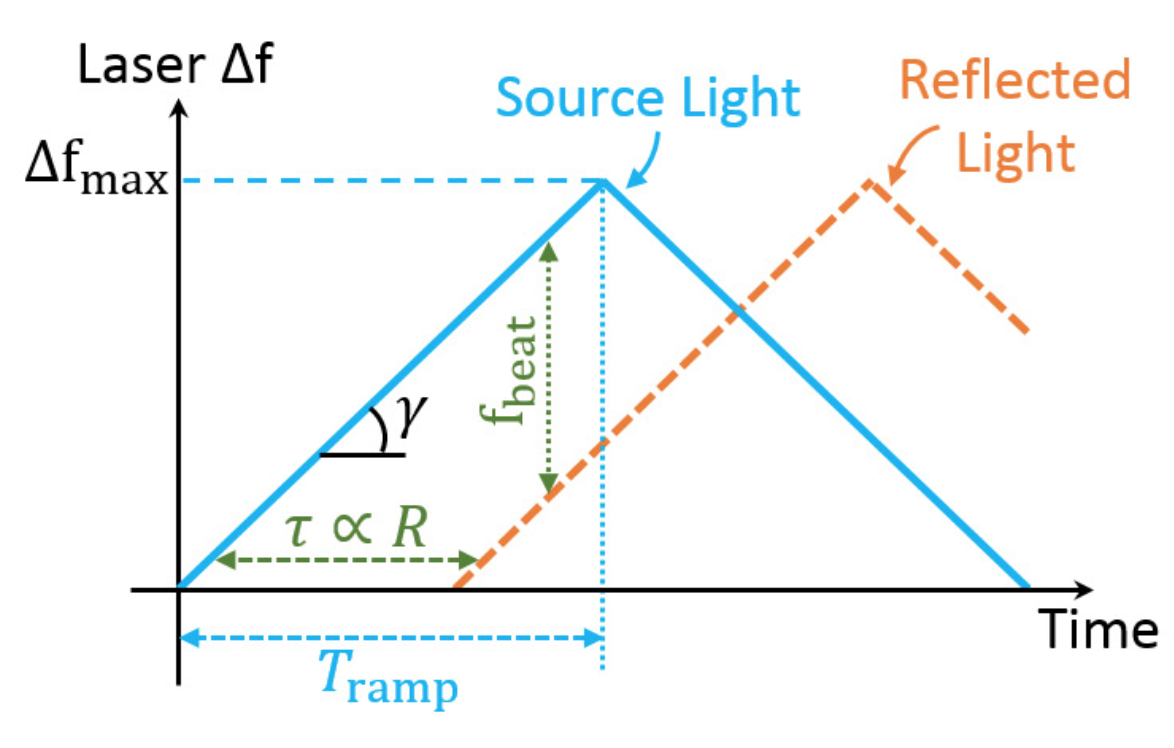
\includegraphics[width=0.5\columnwidth]{figure3}
\caption{Modulation profile of FMCW lidar \cite{behnam}}
\vspace{-0.3in}
\label{lidarsignal}
\end{figure}


As seen from the numerical example in the previous section, solving semidefinite program for line spectral estimation is very expensive in terms of computation complexity (solving a problem of size 200 took almost a minute). Let's see what is the actual size of the sample data in typical lidar system.

Fig. \ref{lidarsignal} \cite{behnam} shows the laser frequency modulation waveform for FMCW lidar (triangular pattern). Typical values of the parameters in this profile for real-world application is as follows.

\begin{itemize}
    \item Desired maximum distance range ($d_{max}$): $10m$
    \item Chirping bandwidth ($\Delta f_{max}$): $10GHz$
    \item Pixel observation window ($T_{ramp}$): $10\mu s$
    \item Chirping rate ($\gamma=\Delta f_{max}/T_{ramp}$): $1PHz/s$
    \item Maximum beating frequency ($f_{beat,max} = 2\gamma d_{max}/c$): $66.7MHz$
    \item Required sampling rate ($f_{sample} = 2f_{beat,max}$): $133MHz$
    \item Number of samples in the time domain ($N_{sample} = T_{obs}f_{sample}$): $1,330$
\end{itemize}

\noindent This shows that the typical size of the problem is $N=1,000\sim10,000$, and it is clear that full-blown semidefinite approach is not an option.

There are two potential approaches for problem simplification. First, we introduced the dual problem formulated as semidefinite program as the original problem was defined in the continuous domain with infinite dimension, and it was impossible to solve such problem numerically. We can still discretize the support space (frequency domain), and the size of that discrete grid is going to be determined by the trade-off between complexity and the resolving power beyond the resolution limit (or super-resolution factor SRF). Then the problem is now formulated on a finite field and the problem size is now $SRF \times N$. There are plenty of $l1$ minimization algorithms, and one of them could potentially show the best performance for given complexity constraint.

Secondly, we can leverage the fact that it is almost always the case that the lidar signal contains only one non-zero tone (or two non-zero tones with complement amplitudes). Multi-path propagation path from the transmitter to receiver is very unlikely since the beamforming antenna for integrated lidar system generally has extremely high directivity \cite{yaacobi}. This introduces another constraint for the original optimization problem, and reduces the size of the optimization space.

\begin{equation}
    \min_{ \tilde{x} }{\| \tilde{x} \|_{1}} \quad \textrm{subject to} \quad \| \tilde{x} \|_0 = 1 \textrm{ and } \| \mathcal{F}_n \tilde{x} - y \|_2 \leq \delta
\end{equation}

There are $SRF \times N$ supports in the optimization space, and we can parallelize the search process of finding the amplitude of minimum magnitude that still satisfies $\| \mathcal{F}_n \tilde{x} - y \|_2 \leq \delta$. After that process, one can simply pick the support with smallest magnitude. 

\begin{figure}[t!]
\centering
            \begin{subfigure}[b]{0.47\columnwidth}
                \centering
		\resizebox{\columnwidth}{!}{
    \huge
    {
    ../../plots/comparison.tex
}
}
\caption{}
\label{fig4a}
\end{subfigure}
\hfill
            \begin{subfigure}[b]{0.47\columnwidth}
                \centering
		\resizebox{\columnwidth}{!}{
            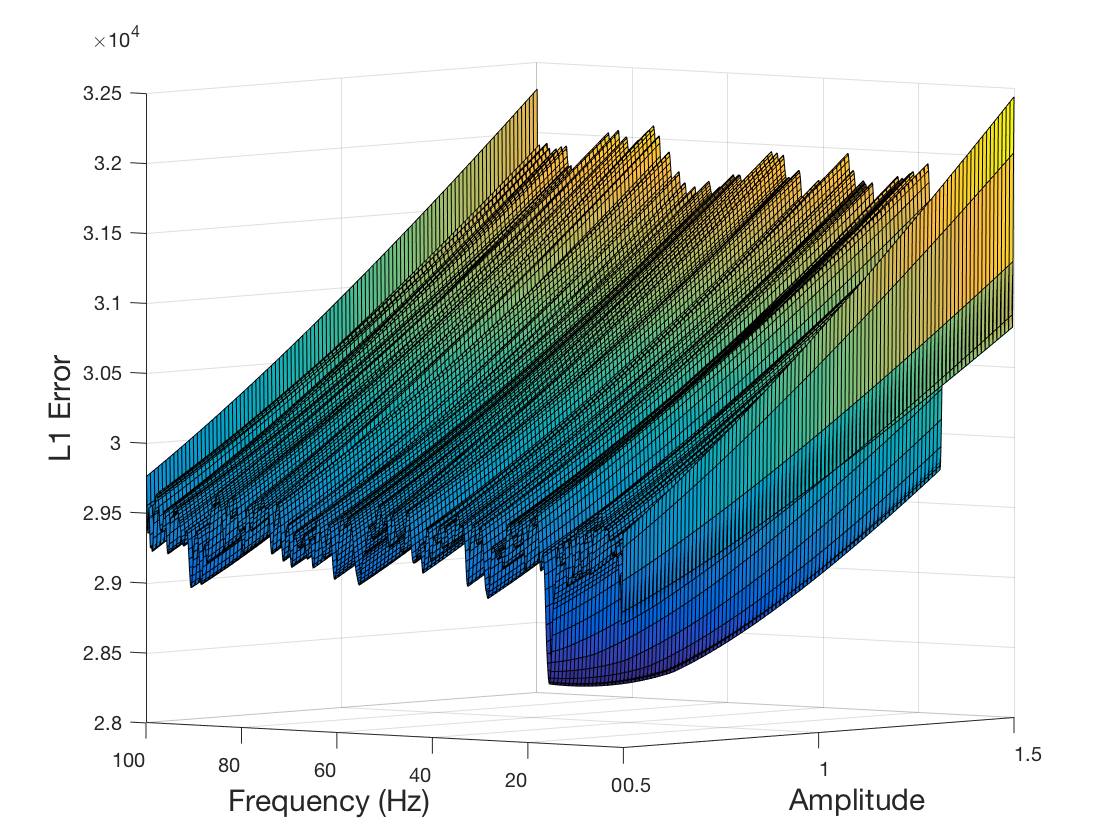
\includegraphics[]{./figures/figure4b.png}
    %\huge
    %{
    %% This file was created by matlab2tikz.
%
%The latest updates can be retrieved from
%  http://www.mathworks.com/matlabcentral/fileexchange/22022-matlab2tikz-matlab2tikz
%where you can also make suggestions and rate matlab2tikz.
%
\begin{tikzpicture}

\begin{axis}[%
width=6.028in,
height=4.754in,
at={(1.011in,0.642in)},
scale only axis,
xmin=0.6,
xmax=1.2,
tick align=outside,
xlabel style={font=\color{white!15!black}},
xlabel={Amplitude},
ymin=0,
ymax=100,
ylabel style={font=\color{white!15!black}},
ylabel={Frequency (Hz)},
zmin=32500,
zmax=36000,
zlabel style={font=\color{white!15!black}},
zlabel={L1 Error},
view={-56.3}{20.4},
axis background/.style={fill=white},
axis x line*=bottom,
axis y line*=left,
axis z line*=left,
xmajorgrids,
ymajorgrids,
zmajorgrids
]

\addplot3[%
surf,
shader=flat corner, draw=black, z buffer=sort, colormap={mymap}{[1pt] rgb(0pt)=(0.2081,0.1663,0.5292); rgb(1pt)=(0.211624,0.189781,0.577676); rgb(2pt)=(0.212252,0.213771,0.626971); rgb(3pt)=(0.2081,0.2386,0.677086); rgb(4pt)=(0.195905,0.264457,0.7279); rgb(5pt)=(0.170729,0.291938,0.779248); rgb(6pt)=(0.125271,0.324243,0.830271); rgb(7pt)=(0.0591333,0.359833,0.868333); rgb(8pt)=(0.0116952,0.38751,0.881957); rgb(9pt)=(0.00595714,0.408614,0.882843); rgb(10pt)=(0.0165143,0.4266,0.878633); rgb(11pt)=(0.0328524,0.443043,0.871957); rgb(12pt)=(0.0498143,0.458571,0.864057); rgb(13pt)=(0.0629333,0.47369,0.855438); rgb(14pt)=(0.0722667,0.488667,0.8467); rgb(15pt)=(0.0779429,0.503986,0.838371); rgb(16pt)=(0.0793476,0.520024,0.831181); rgb(17pt)=(0.0749429,0.537543,0.826271); rgb(18pt)=(0.0640571,0.556986,0.823957); rgb(19pt)=(0.0487714,0.577224,0.822829); rgb(20pt)=(0.0343429,0.596581,0.819852); rgb(21pt)=(0.0265,0.6137,0.8135); rgb(22pt)=(0.0238905,0.628662,0.803762); rgb(23pt)=(0.0230905,0.641786,0.791267); rgb(24pt)=(0.0227714,0.653486,0.776757); rgb(25pt)=(0.0266619,0.664195,0.760719); rgb(26pt)=(0.0383714,0.674271,0.743552); rgb(27pt)=(0.0589714,0.683757,0.725386); rgb(28pt)=(0.0843,0.692833,0.706167); rgb(29pt)=(0.113295,0.7015,0.685857); rgb(30pt)=(0.145271,0.709757,0.664629); rgb(31pt)=(0.180133,0.717657,0.642433); rgb(32pt)=(0.217829,0.725043,0.619262); rgb(33pt)=(0.258643,0.731714,0.595429); rgb(34pt)=(0.302171,0.737605,0.571186); rgb(35pt)=(0.348167,0.742433,0.547267); rgb(36pt)=(0.395257,0.7459,0.524443); rgb(37pt)=(0.44201,0.748081,0.503314); rgb(38pt)=(0.487124,0.749062,0.483976); rgb(39pt)=(0.530029,0.749114,0.466114); rgb(40pt)=(0.570857,0.748519,0.44939); rgb(41pt)=(0.609852,0.747314,0.433686); rgb(42pt)=(0.6473,0.7456,0.4188); rgb(43pt)=(0.683419,0.743476,0.404433); rgb(44pt)=(0.71841,0.741133,0.390476); rgb(45pt)=(0.752486,0.7384,0.376814); rgb(46pt)=(0.785843,0.735567,0.363271); rgb(47pt)=(0.818505,0.732733,0.34979); rgb(48pt)=(0.850657,0.7299,0.336029); rgb(49pt)=(0.882433,0.727433,0.3217); rgb(50pt)=(0.913933,0.725786,0.306276); rgb(51pt)=(0.944957,0.726114,0.288643); rgb(52pt)=(0.973895,0.731395,0.266648); rgb(53pt)=(0.993771,0.745457,0.240348); rgb(54pt)=(0.999043,0.765314,0.216414); rgb(55pt)=(0.995533,0.786057,0.196652); rgb(56pt)=(0.988,0.8066,0.179367); rgb(57pt)=(0.978857,0.827143,0.163314); rgb(58pt)=(0.9697,0.848138,0.147452); rgb(59pt)=(0.962586,0.870514,0.1309); rgb(60pt)=(0.958871,0.8949,0.113243); rgb(61pt)=(0.959824,0.921833,0.0948381); rgb(62pt)=(0.9661,0.951443,0.0755333); rgb(63pt)=(0.9763,0.9831,0.0538)}, mesh/rows=21]
table[row sep=crcr, point meta=\thisrow{c}] {%
%
x	y	z	c\\
0.6	0	34465.0059952326	34465.0059952326\\
0.6	0.1	34329.9100711035	34329.9100711035\\
0.6	0.2	34048.286638357	34048.286638357\\
0.6	0.3	33832.8087653496	33832.8087653496\\
0.6	0.4	33802.1606971248	33802.1606971248\\
0.6	0.5	33920.5310257882	33920.5310257882\\
0.6	0.6	34041.9548180324	34041.9548180324\\
0.6	0.7	34023.6473597595	34023.6473597595\\
0.6	0.8	33976.4712032693	33976.4712032693\\
0.6	0.9	33985.617067332	33985.617067332\\
0.6	1	34047.7940003549	34047.7940003549\\
0.6	1.1	34142.9790785705	34142.9790785705\\
0.6	1.2	34171.9179934759	34171.9179934759\\
0.6	1.3	34141.1597235108	34141.1597235108\\
0.6	1.4	34102.0617475414	34102.0617475414\\
0.6	1.5	34086.0668943218	34086.0668943218\\
0.6	1.6	34097.818027094	34097.818027094\\
0.6	1.7	34073.1913154283	34073.1913154283\\
0.6	1.8	34022.531812963	34022.531812963\\
0.6	1.9	33983.1418461794	33983.1418461794\\
0.6	2	33976.8738664932	33976.8738664932\\
0.6	2.1	34005.7807384179	34005.7807384179\\
0.6	2.2	34052.2490874462	34052.2490874462\\
0.6	2.3	34038.5123142597	34038.5123142597\\
0.6	2.4	33987.3343237758	33987.3343237758\\
0.6	2.5	33957.5209568822	33957.5209568822\\
0.6	2.6	33947.7123808359	33947.7123808359\\
0.6	2.7	33896.933055333	33896.933055333\\
0.6	2.8	33804.9007634264	33804.9007634264\\
0.6	2.9	33704.3991611282	33704.3991611282\\
0.6	3	33640.8652955449	33640.8652955449\\
0.6	3.1	33615.0105142382	33615.0105142382\\
0.6	3.2	33603.7709828523	33603.7709828523\\
0.6	3.3	33561.7530614678	33561.7530614678\\
0.6	3.4	33503.5964544859	33503.5964544859\\
0.6	3.5	33492.1425268355	33492.1425268355\\
0.6	3.6	33506.6926332885	33506.6926332885\\
0.6	3.7	33490.2614280801	33490.2614280801\\
0.6	3.8	33452.6710610187	33452.6710610187\\
0.6	3.9	33431.926238344	33431.926238344\\
0.6	4	33452.142878101	33452.142878101\\
0.6	4.1	33499.0538451278	33499.0538451278\\
0.6	4.2	33548.0149367074	33548.0149367074\\
0.6	4.3	33576.911459081	33576.911459081\\
0.6	4.4	33601.1307832187	33601.1307832187\\
0.6	4.5	33642.2652269229	33642.2652269229\\
0.6	4.6	33677.4299731747	33677.4299731747\\
0.6	4.7	33667.8799203896	33667.8799203896\\
0.6	4.8	33650.5984639715	33650.5984639715\\
0.6	4.9	33654.4573384657	33654.4573384657\\
0.6	5	33691.6017712061	33691.6017712061\\
0.6	5.1	33751.2585923398	33751.2585923398\\
0.6	5.2	33819.1169676405	33819.1169676405\\
0.6	5.3	33879.4494966242	33879.4494966242\\
0.6	5.4	33936.3117373926	33936.3117373926\\
0.6	5.5	33995.7479269832	33995.7479269832\\
0.6	5.6	34044.8617014613	34044.8617014613\\
0.6	5.7	34053.2010343553	34053.2010343553\\
0.6	5.8	34025.0046398817	34025.0046398817\\
0.6	5.9	33977.5353455085	33977.5353455085\\
0.6	6	33932.5834016897	33932.5834016897\\
0.6	6.1	33904.6863392524	33904.6863392524\\
0.6	6.2	33889.3178735422	33889.3178735422\\
0.6	6.3	33881.1546990434	33881.1546990434\\
0.6	6.4	33886.9289366435	33886.9289366435\\
0.6	6.5	33915.1120967993	33915.1120967993\\
0.6	6.6	33961.1146307373	33961.1146307373\\
0.6	6.7	34018.0970201212	34018.0970201212\\
0.6	6.8	34068.917770889	34068.917770889\\
0.6	6.9	34087.8774539762	34087.8774539762\\
0.6	7	34095.8784426893	34095.8784426893\\
0.6	7.1	34094.0200727402	34094.0200727402\\
0.6	7.2	34083.0849656348	34083.0849656348\\
0.6	7.3	34060.6996943373	34060.6996943373\\
0.6	7.4	34035.1327735414	34035.1327735414\\
0.6	7.5	34017.2921636079	34017.2921636079\\
0.6	7.6	34007.4249223998	34007.4249223998\\
0.6	7.7	34014.1929842143	34014.1929842143\\
0.6	7.8	34040.2900537172	34040.2900537172\\
0.6	7.9	34061.9621140624	34061.9621140624\\
0.6	8	34105.3095121871	34105.3095121871\\
0.6	8.1	34153.9836428913	34153.9836428913\\
0.6	8.2	34176.7389892845	34176.7389892845\\
0.6	8.3	34170.9940565677	34170.9940565677\\
0.6	8.4	34137.8750823521	34137.8750823521\\
0.6	8.5	34095.0507835424	34095.0507835424\\
0.6	8.6	34048.1314429246	34048.1314429246\\
0.6	8.7	33988.2836479971	33988.2836479971\\
0.6	8.8	33913.3886835918	33913.3886835918\\
0.6	8.9	33821.6130956044	33821.6130956044\\
0.6	9	33742.3952799857	33742.3952799857\\
0.6	9.1	33709.5044651459	33709.5044651459\\
0.6	9.2	33680.4497216491	33680.4497216491\\
0.6	9.3	33637.9333269197	33637.9333269197\\
0.6	9.4	33604.7685104562	33604.7685104562\\
0.6	9.5	33605.8172424315	33605.8172424315\\
0.6	9.6	33647.7267540998	33647.7267540998\\
0.6	9.7	33708.4939419221	33708.4939419221\\
0.6	9.8	33758.7550084186	33758.7550084186\\
0.6	9.9	33795.7090200184	33795.7090200184\\
0.6	10	33815.1855264329	33815.1855264329\\
0.6	10.1	33835.4990566428	33835.4990566428\\
0.6	10.2	33825.3362038985	33825.3362038985\\
0.6	10.3	33769.3418204869	33769.3418204869\\
0.6	10.4	33688.9873685439	33688.9873685439\\
0.6	10.5	33611.9626448592	33611.9626448592\\
0.6	10.6	33559.6741362406	33559.6741362406\\
0.6	10.7	33533.4420724821	33533.4420724821\\
0.6	10.8	33532.3377244051	33532.3377244051\\
0.6	10.9	33548.0273510417	33548.0273510417\\
0.6	11	33586.3565604439	33586.3565604439\\
0.6	11.1	33656.3316965314	33656.3316965314\\
0.6	11.2	33727.6279249602	33727.6279249602\\
0.6	11.3	33768.2820010661	33768.2820010661\\
0.6	11.4	33772.6568208596	33772.6568208596\\
0.6	11.5	33766.4355284835	33766.4355284835\\
0.6	11.6	33757.9192307643	33757.9192307643\\
0.6	11.7	33747.080701155	33747.080701155\\
0.6	11.8	33746.6064316166	33746.6064316166\\
0.6	11.9	33745.7991437575	33745.7991437575\\
0.6	12	33749.776680741	33749.776680741\\
0.6	12.1	33761.1914459426	33761.1914459426\\
0.6	12.2	33770.8278045113	33770.8278045113\\
0.6	12.3	33757.6033362436	33757.6033362436\\
0.6	12.4	33724.772575722	33724.772575722\\
0.6	12.5	33693.8497890255	33693.8497890255\\
0.6	12.6	33667.245744906	33667.245744906\\
0.6	12.7	33647.4518116879	33647.4518116879\\
0.6	12.8	33653.5901806666	33653.5901806666\\
0.6	12.9	33685.451423743	33685.451423743\\
0.6	13	33738.1270496906	33738.1270496906\\
0.6	13.1	33807.0074232118	33807.0074232118\\
0.6	13.2	33877.4810162	33877.4810162\\
0.6	13.3	33925.5940200494	33925.5940200494\\
0.6	13.4	33946.5151120532	33946.5151120532\\
0.6	13.5	33954.0142443954	33954.0142443954\\
0.6	13.6	33963.3279633266	33963.3279633266\\
0.6	13.7	33967.2887741206	33967.2887741206\\
0.6	13.8	33958.5232721066	33958.5232721066\\
0.6	13.9	33939.8721445261	33939.8721445261\\
0.6	14	33918.6391658398	33918.6391658398\\
0.6	14.1	33899.9300185083	33899.9300185083\\
0.6	14.2	33879.3061846724	33879.3061846724\\
0.6	14.3	33840.8137279896	33840.8137279896\\
0.6	14.4	33783.0746783017	33783.0746783017\\
0.6	14.5	33714.3073877489	33714.3073877489\\
0.6	14.6	33642.2904532569	33642.2904532569\\
0.6	14.7	33562.6830197797	33562.6830197797\\
0.6	14.8	33449.0771097906	33449.0771097906\\
0.6	14.9	33286.7160951861	33286.7160951861\\
0.6	15	33105.9556856348	33105.9556856348\\
0.6	15.1	32928.8371123706	32928.8371123706\\
0.6	15.2	32814.0724829169	32814.0724829169\\
0.6	15.3	32714.7308544014	32714.7308544014\\
0.6	15.4	32632.35169194	32632.35169194\\
0.6	15.5	32575.8120458628	32575.8120458628\\
0.6	15.6	32557.0230364296	32557.0230364296\\
0.6	15.7	32580.8903296093	32580.8903296093\\
0.6	15.8	32632.5926809303	32632.5926809303\\
0.6	15.9	32685.2090908353	32685.2090908353\\
0.6	16	32752.7295324202	32752.7295324202\\
0.6	16.1	32839.730802844	32839.730802844\\
0.6	16.2	32956.3935170865	32956.3935170865\\
0.6	16.3	33104.3261592844	33104.3261592844\\
0.6	16.4	33240.5242990126	33240.5242990126\\
0.6	16.5	33357.9402585991	33357.9402585991\\
0.6	16.6	33453.3446049321	33453.3446049321\\
0.6	16.7	33528.9107409545	33528.9107409545\\
0.6	16.8	33589.9830236068	33589.9830236068\\
0.6	16.9	33629.5868280023	33629.5868280023\\
0.6	17	33656.0477787924	33656.0477787924\\
0.6	17.1	33673.7747642707	33673.7747642707\\
0.6	17.2	33676.9558051588	33676.9558051588\\
0.6	17.3	33658.5062994793	33658.5062994793\\
0.6	17.4	33620.7806612715	33620.7806612715\\
0.6	17.5	33567.1186756465	33567.1186756465\\
0.6	17.6	33507.8725615058	33507.8725615058\\
0.6	17.7	33455.2693415323	33455.2693415323\\
0.6	17.8	33425.7506464435	33425.7506464435\\
0.6	17.9	33416.0527901874	33416.0527901874\\
0.6	18	33430.7877305065	33430.7877305065\\
0.6	18.1	33470.3888717814	33470.3888717814\\
0.6	18.2	33523.8571834704	33523.8571834704\\
0.6	18.3	33580.4540867007	33580.4540867007\\
0.6	18.4	33638.6209137249	33638.6209137249\\
0.6	18.5	33699.3059909811	33699.3059909811\\
0.6	18.6	33756.9030476723	33756.9030476723\\
0.6	18.7	33802.6699461489	33802.6699461489\\
0.6	18.8	33833.7127754455	33833.7127754455\\
0.6	18.9	33851.0451993497	33851.0451993497\\
0.6	19	33857.3668013003	33857.3668013003\\
0.6	19.1	33855.1277425461	33855.1277425461\\
0.6	19.2	33841.1507298667	33841.1507298667\\
0.6	19.3	33812.7491343277	33812.7491343277\\
0.6	19.4	33772.1700530213	33772.1700530213\\
0.6	19.5	33725.8631662129	33725.8631662129\\
0.6	19.6	33680.5827593281	33680.5827593281\\
0.6	19.7	33645.1726180821	33645.1726180821\\
0.6	19.8	33621.1901252411	33621.1901252411\\
0.6	19.9	33601.7329347865	33601.7329347865\\
0.6	20	33586.5610100073	33586.5610100073\\
0.6	20.1	33582.2996705237	33582.2996705237\\
0.6	20.2	33584.3950766692	33584.3950766692\\
0.6	20.3	33587.4623162967	33587.4623162967\\
0.6	20.4	33589.3959288158	33589.3959288158\\
0.6	20.5	33588.438582029	33588.438582029\\
0.6	20.6	33586.500104898	33586.500104898\\
0.6	20.7	33582.4842355262	33582.4842355262\\
0.6	20.8	33589.2458443114	33589.2458443114\\
0.6	20.9	33603.8472245716	33603.8472245716\\
0.6	21	33628.4834655943	33628.4834655943\\
0.6	21.1	33663.6040900662	33663.6040900662\\
0.6	21.2	33703.6818211746	33703.6818211746\\
0.6	21.3	33744.1626299724	33744.1626299724\\
0.6	21.4	33782.1373738991	33782.1373738991\\
0.6	21.5	33814.0491756731	33814.0491756731\\
0.6	21.6	33838.7916924491	33838.7916924491\\
0.6	21.7	33848.6569915734	33848.6569915734\\
0.6	21.8	33838.0314550188	33838.0314550188\\
0.6	21.9	33811.8796437904	33811.8796437904\\
0.6	22	33779.4906261447	33779.4906261447\\
0.6	22.1	33745.4229178764	33745.4229178764\\
0.6	22.2	33711.3707329706	33711.3707329706\\
0.6	22.3	33683.2036593315	33683.2036593315\\
0.6	22.4	33667.8388353952	33667.8388353952\\
0.6	22.5	33667.376856036	33667.376856036\\
0.6	22.6	33683.6887213769	33683.6887213769\\
0.6	22.7	33723.9021723491	33723.9021723491\\
0.6	22.8	33775.8350181129	33775.8350181129\\
0.6	22.9	33814.080007736	33814.080007736\\
0.6	23	33842.8177626487	33842.8177626487\\
0.6	23.1	33861.0580197955	33861.0580197955\\
0.6	23.2	33863.1725160891	33863.1725160891\\
0.6	23.3	33850.0812687643	33850.0812687643\\
0.6	23.4	33824.9125255085	33824.9125255085\\
0.6	23.5	33796.8956301662	33796.8956301662\\
0.6	23.6	33759.9914016819	33759.9914016819\\
0.6	23.7	33732.7520982236	33732.7520982236\\
0.6	23.8	33728.2279690585	33728.2279690585\\
0.6	23.9	33739.2785414842	33739.2785414842\\
0.6	24	33760.2475734302	33760.2475734302\\
0.6	24.1	33798.4765604734	33798.4765604734\\
0.6	24.2	33842.5102488163	33842.5102488163\\
0.6	24.3	33886.0008879636	33886.0008879636\\
0.6	24.4	33925.3280801834	33925.3280801834\\
0.6	24.5	33958.9993520611	33958.9993520611\\
0.6	24.6	33981.3323225015	33981.3323225015\\
0.6	24.7	33984.5800548195	33984.5800548195\\
0.6	24.8	33967.4059069297	33967.4059069297\\
0.6	24.9	33934.346943461	33934.346943461\\
0.6	25	33887.8043621395	33887.8043621395\\
0.6	25.1	33844.8337162031	33844.8337162031\\
0.6	25.2	33813.6119964796	33813.6119964796\\
0.6	25.3	33796.349459996	33796.349459996\\
0.6	25.4	33796.1342207638	33796.1342207638\\
0.6	25.5	33816.4661986674	33816.4661986674\\
0.6	25.6	33856.8563418743	33856.8563418743\\
0.6	25.7	33921.7913252431	33921.7913252431\\
0.6	25.8	33980.1483314491	33980.1483314491\\
0.6	25.9	34018.8868191053	34018.8868191053\\
0.6	26	34041.3520794587	34041.3520794587\\
0.6	26.1	34046.0108714447	34046.0108714447\\
0.6	26.2	34033.3160027667	34033.3160027667\\
0.6	26.3	34006.3812949792	34006.3812949792\\
0.6	26.4	33970.446711652	33970.446711652\\
0.6	26.5	33932.5979292117	33932.5979292117\\
0.6	26.6	33895.7039039583	33895.7039039583\\
0.6	26.7	33862.6259005038	33862.6259005038\\
0.6	26.8	33828.3314188964	33828.3314188964\\
0.6	26.9	33787.8158583405	33787.8158583405\\
0.6	27	33745.6491978699	33745.6491978699\\
0.6	27.1	33710.8203111308	33710.8203111308\\
0.6	27.2	33665.7624296495	33665.7624296495\\
0.6	27.3	33613.0434868169	33613.0434868169\\
0.6	27.4	33568.2245129663	33568.2245129663\\
0.6	27.5	33542.9514978123	33542.9514978123\\
0.6	27.6	33543.345117224	33543.345117224\\
0.6	27.7	33567.4404292887	33567.4404292887\\
0.6	27.8	33610.6939397547	33610.6939397547\\
0.6	27.9	33660.330540534	33660.330540534\\
0.6	28	33710.0516158529	33710.0516158529\\
0.6	28.1	33760.7093410973	33760.7093410973\\
0.6	28.2	33803.5435245356	33803.5435245356\\
0.6	28.3	33831.914270176	33831.914270176\\
0.6	28.4	33843.6624907907	33843.6624907907\\
0.6	28.5	33847.4775159012	33847.4775159012\\
0.6	28.6	33848.8206653125	33848.8206653125\\
0.6	28.7	33849.6278327629	33849.6278327629\\
0.6	28.8	33852.2793357349	33852.2793357349\\
0.6	28.9	33853.8331100997	33853.8331100997\\
0.6	29	33853.7338955945	33853.7338955945\\
0.6	29.1	33850.1175432481	33850.1175432481\\
0.6	29.2	33837.8285483095	33837.8285483095\\
0.6	29.3	33806.4605985582	33806.4605985582\\
0.6	29.4	33756.2476687673	33756.2476687673\\
0.6	29.5	33694.2798502017	33694.2798502017\\
0.6	29.6	33624.8668488738	33624.8668488738\\
0.6	29.7	33553.2494359079	33553.2494359079\\
0.6	29.8	33491.8687184795	33491.8687184795\\
0.6	29.9	33452.1460196083	33452.1460196083\\
0.6	30	33442.6841265191	33442.6841265191\\
0.6	30.1	33465.3491040746	33465.3491040746\\
0.6	30.2	33514.4387579927	33514.4387579927\\
0.6	30.3	33577.3003647603	33577.3003647603\\
0.6	30.4	33643.5795247556	33643.5795247556\\
0.6	30.5	33704.8698901176	33704.8698901176\\
0.6	30.6	33757.0069772944	33757.0069772944\\
0.6	30.7	33792.1465203462	33792.1465203462\\
0.6	30.8	33807.7126746585	33807.7126746585\\
0.6	30.9	33806.8561609273	33806.8561609273\\
0.6	31	33794.6094370397	33794.6094370397\\
0.6	31.1	33774.6772485643	33774.6772485643\\
0.6	31.2	33748.2541950992	33748.2541950992\\
0.6	31.3	33717.9547439883	33717.9547439883\\
0.6	31.4	33690.760504774	33690.760504774\\
0.6	31.5	33672.765317384	33672.765317384\\
0.6	31.6	33667.6181791118	33667.6181791118\\
0.6	31.7	33671.6778352082	33671.6778352082\\
0.6	31.8	33683.2998709633	33683.2998709633\\
0.6	31.9	33702.9347314617	33702.9347314617\\
0.6	32	33726.1534966929	33726.1534966929\\
0.6	32.1	33744.7308175065	33744.7308175065\\
0.6	32.2	33750.2575621505	33750.2575621505\\
0.6	32.3	33739.412937561	33739.412937561\\
0.6	32.4	33718.0426348645	33718.0426348645\\
0.6	32.5	33693.5087517298	33693.5087517298\\
0.6	32.6	33669.8629552982	33669.8629552982\\
0.6	32.7	33643.9387310585	33643.9387310585\\
0.6	32.8	33615.7912201935	33615.7912201935\\
0.6	32.9	33590.0417542455	33590.0417542455\\
0.6	33	33570.5050934191	33570.5050934191\\
0.6	33.1	33554.753136314	33554.753136314\\
0.6	33.2	33534.2861876947	33534.2861876947\\
0.6	33.3	33502.2808643987	33502.2808643987\\
0.6	33.4	33467.3519127435	33467.3519127435\\
0.6	33.5	33448.3279255898	33448.3279255898\\
0.6	33.6	33451.5064682433	33451.5064682433\\
0.6	33.7	33468.555051253	33468.555051253\\
0.6	33.8	33496.3050384368	33496.3050384368\\
0.6	33.9	33537.3592864721	33537.3592864721\\
0.6	34	33592.8643805722	33592.8643805722\\
0.6	34.1	33655.440663853	33655.440663853\\
0.6	34.2	33710.7911844681	33710.7911844681\\
0.6	34.3	33747.8612267995	33747.8612267995\\
0.6	34.4	33760.8309297745	33760.8309297745\\
0.6	34.5	33747.7317656777	33747.7317656777\\
0.6	34.6	33712.0954635191	33712.0954635191\\
0.6	34.7	33651.7678132348	33651.7678132348\\
0.6	34.8	33568.4207812997	33568.4207812997\\
0.6	34.9	33476.0945731164	33476.0945731164\\
0.6	35	33395.4801036544	33395.4801036544\\
0.6	35.1	33339.3354813186	33339.3354813186\\
0.6	35.2	33308.9440162597	33308.9440162597\\
0.6	35.3	33304.6512652722	33304.6512652722\\
0.6	35.4	33326.9305871113	33326.9305871113\\
0.6	35.5	33374.051159567	33374.051159567\\
0.6	35.6	33443.4517913873	33443.4517913873\\
0.6	35.7	33508.9767786654	33508.9767786654\\
0.6	35.8	33546.9035373319	33546.9035373319\\
0.6	35.9	33555.5452664795	33555.5452664795\\
0.6	36	33549.3009096881	33549.3009096881\\
0.6	36.1	33545.1355690845	33545.1355690845\\
0.6	36.2	33539.7985212193	33539.7985212193\\
0.6	36.3	33533.7675423427	33533.7675423427\\
0.6	36.4	33534.4748283872	33534.4748283872\\
0.6	36.5	33547.4641342123	33547.4641342123\\
0.6	36.6	33578.402227387	33578.402227387\\
0.6	36.7	33629.5939460154	33629.5939460154\\
0.6	36.8	33678.657575767	33678.657575767\\
0.6	36.9	33718.1330937202	33718.1330937202\\
0.6	37	33743.9386964804	33743.9386964804\\
0.6	37.1	33749.3952018652	33749.3952018652\\
0.6	37.2	33725.2577030464	33725.2577030464\\
0.6	37.3	33668.2558062138	33668.2558062138\\
0.6	37.4	33580.5271823221	33580.5271823221\\
0.6	37.5	33481.0591590712	33481.0591590712\\
0.6	37.6	33376.0967124018	33376.0967124018\\
0.6	37.7	33317.2015760219	33317.2015760219\\
0.6	37.8	33298.612187227	33298.612187227\\
0.6	37.9	33323.5298528262	33323.5298528262\\
0.6	38	33392.0757353917	33392.0757353917\\
0.6	38.1	33495.5715610632	33495.5715610632\\
0.6	38.2	33618.0963584652	33618.0963584652\\
0.6	38.3	33731.092559502	33731.092559502\\
0.6	38.4	33816.7910795849	33816.7910795849\\
0.6	38.5	33875.828392194	33875.828392194\\
0.6	38.6	33906.6185291517	33906.6185291517\\
0.6	38.7	33913.9261643304	33913.9261643304\\
0.6	38.8	33905.6966171136	33905.6966171136\\
0.6	38.9	33892.227082576	33892.227082576\\
0.6	39	33882.2019580968	33882.2019580968\\
0.6	39.1	33879.1304460368	33879.1304460368\\
0.6	39.2	33884.2437457132	33884.2437457132\\
0.6	39.3	33896.854867627	33896.854867627\\
0.6	39.4	33913.0564607204	33913.0564607204\\
0.6	39.5	33930.4043988702	33930.4043988702\\
0.6	39.6	33949.5044421976	33949.5044421976\\
0.6	39.7	33983.5308225659	33983.5308225659\\
0.6	39.8	33992.9209588049	33992.9209588049\\
0.6	39.9	33993.1864748102	33993.1864748102\\
0.6	40	33987.950508525	33987.950508525\\
0.6	40.1	33983.6726058304	33983.6726058304\\
0.6	40.2	33982.4200260729	33982.4200260729\\
0.6	40.3	33987.9124339013	33987.9124339013\\
0.6	40.4	34002.247770648	34002.247770648\\
0.6	40.5	34023.4350241712	34023.4350241712\\
0.6	40.6	34047.7562212983	34047.7562212983\\
0.6	40.7	34080.505668152	34080.505668152\\
0.6	40.8	34105.7136921372	34105.7136921372\\
0.6	40.9	34111.9221135249	34111.9221135249\\
0.6	41	34101.3580440924	34101.3580440924\\
0.6	41.1	34076.2283039664	34076.2283039664\\
0.6	41.2	34039.9358656868	34039.9358656868\\
0.6	41.3	33999.1680331166	33999.1680331166\\
0.6	41.4	33964.238741574	33964.238741574\\
0.6	41.5	33940.9581196006	33940.9581196006\\
0.6	41.6	33930.9080310508	33930.9080310508\\
0.6	41.7	33939.4430593185	33939.4430593185\\
0.6	41.8	33963.2793412646	33963.2793412646\\
0.6	41.9	33983.4017507037	33983.4017507037\\
0.6	42	33996.7781896465	33996.7781896465\\
0.6	42.1	34003.0806222029	34003.0806222029\\
0.6	42.2	33999.5948048918	33999.5948048918\\
0.6	42.3	33986.2261493733	33986.2261493733\\
0.6	42.4	33965.838406662	33965.838406662\\
0.6	42.5	33947.0744783227	33947.0744783227\\
0.6	42.6	33934.041849656	33934.041849656\\
0.6	42.7	33927.5976995468	33927.5976995468\\
0.6	42.8	33932.3056094661	33932.3056094661\\
0.6	42.9	33939.0469117045	33939.0469117045\\
0.6	43	33947.0817057349	33947.0817057349\\
0.6	43.1	33956.8322565224	33956.8322565224\\
0.6	43.2	33968.793513242	33968.793513242\\
0.6	43.3	33981.6534721953	33981.6534721953\\
0.6	43.4	33992.0762222939	33992.0762222939\\
0.6	43.5	33995.5931943153	33995.5931943153\\
0.6	43.6	33988.9422208865	33988.9422208865\\
0.6	43.7	33972.0671831398	33972.0671831398\\
0.6	43.8	33950.1978950186	33950.1978950186\\
0.6	43.9	33922.0787472833	33922.0787472833\\
0.6	44	33887.7911978319	33887.7911978319\\
0.6	44.1	33849.4006586247	33849.4006586247\\
0.6	44.2	33807.7460174252	33807.7460174252\\
0.6	44.3	33763.1406197742	33763.1406197742\\
0.6	44.4	33715.0700449048	33715.0700449048\\
0.6	44.5	33663.9282949605	33663.9282949605\\
0.6	44.6	33599.8932791075	33599.8932791075\\
0.6	44.7	33526.2909728818	33526.2909728818\\
0.6	44.8	33448.6302028617	33448.6302028617\\
0.6	44.9	33397.7574671411	33397.7574671411\\
0.6	45	33373.571931687	33373.571931687\\
0.6	45.1	33383.5103318372	33383.5103318372\\
0.6	45.2	33427.4628337927	33427.4628337927\\
0.6	45.3	33499.4137316299	33499.4137316299\\
0.6	45.4	33592.444419361	33592.444419361\\
0.6	45.5	33693.4353535413	33693.4353535413\\
0.6	45.6	33787.2012096622	33787.2012096622\\
0.6	45.7	33857.0512492869	33857.0512492869\\
0.6	45.8	33892.5488784647	33892.5488784647\\
0.6	45.9	33888.2639289339	33888.2639289339\\
0.6	46	33856.992098598	33856.992098598\\
0.6	46.1	33808.7696965455	33808.7696965455\\
0.6	46.2	33753.4454851531	33753.4454851531\\
0.6	46.3	33706.0639074563	33706.0639074563\\
0.6	46.4	33681.6991622798	33681.6991622798\\
0.6	46.5	33692.7977539916	33692.7977539916\\
0.6	46.6	33734.3274318678	33734.3274318678\\
0.6	46.7	33794.2479573567	33794.2479573567\\
0.6	46.8	33865.6604711159	33865.6604711159\\
0.6	46.9	33946.468602085	33946.468602085\\
0.6	47	34001.05695024	34001.05695024\\
0.6	47.1	34029.066535712	34029.066535712\\
0.6	47.2	34033.8603171823	34033.8603171823\\
0.6	47.3	34023.8643346677	34023.8643346677\\
0.6	47.4	34000.7382845686	34000.7382845686\\
0.6	47.5	33967.1805766264	33967.1805766264\\
0.6	47.6	33924.5685880413	33924.5685880413\\
0.6	47.7	33871.4538107449	33871.4538107449\\
0.6	47.8	33806.8345269316	33806.8345269316\\
0.6	47.9	33736.6356946385	33736.6356946385\\
0.6	48	33665.5504129481	33665.5504129481\\
0.6	48.1	33598.2338475896	33598.2338475896\\
0.6	48.2	33542.9661646988	33542.9661646988\\
0.6	48.3	33513.7872001979	33513.7872001979\\
0.6	48.4	33521.26041161	33521.26041161\\
0.6	48.5	33556.3220414675	33556.3220414675\\
0.6	48.6	33613.4700034805	33613.4700034805\\
0.6	48.7	33683.3650049975	33683.3650049975\\
0.6	48.8	33751.3486393752	33751.3486393752\\
0.6	48.9	33810.1827109951	33810.1827109951\\
0.6	49	33861.5029083186	33861.5029083186\\
0.6	49.1	33905.3731623496	33905.3731623496\\
0.6	49.2	33933.0453030234	33933.0453030234\\
0.6	49.3	33949.3598254343	33949.3598254343\\
0.6	49.4	33954.7475043285	33954.7475043285\\
0.6	49.5	33946.3153586505	33946.3153586505\\
0.6	49.6	33923.4796928061	33923.4796928061\\
0.6	49.7	33885.5782089495	33885.5782089495\\
0.6	49.8	33834.1918593152	33834.1918593152\\
0.6	49.9	33773.3709503066	33773.3709503066\\
0.6	50	33713.5453005036	33713.5453005036\\
0.6	50.1	33679.1540812296	33679.1540812296\\
0.6	50.2	33665.0297035348	33665.0297035348\\
0.6	50.3	33686.6636689841	33686.6636689841\\
0.6	50.4	33736.5611101524	33736.5611101524\\
0.6	50.5	33796.0893191067	33796.0893191067\\
0.6	50.6	33859.6557557226	33859.6557557226\\
0.6	50.7	33917.2828155861	33917.2828155861\\
0.6	50.8	33963.0954484012	33963.0954484012\\
0.6	50.9	33991.2944942126	33991.2944942126\\
0.6	51	34003.483096424	34003.483096424\\
0.6	51.1	34016.0914101949	34016.0914101949\\
0.6	51.2	34043.8349644268	34043.8349644268\\
0.6	51.3	34074.5095991299	34074.5095991299\\
0.6	51.4	34107.9631721103	34107.9631721103\\
0.6	51.5	34135.974755749	34135.974755749\\
0.6	51.6	34150.2153003791	34150.2153003791\\
0.6	51.7	34151.1669780037	34151.1669780037\\
0.6	51.8	34140.5161436384	34140.5161436384\\
0.6	51.9	34116.5687405854	34116.5687405854\\
0.6	52	34084.1106650209	34084.1106650209\\
0.6	52.1	34043.8733976501	34043.8733976501\\
0.6	52.2	34016.0816574426	34016.0816574426\\
0.6	52.3	33995.7180694622	33995.7180694622\\
0.6	52.4	33966.4553951324	33966.4553951324\\
0.6	52.5	33924.9440205863	33924.9440205863\\
0.6	52.6	33874.3876941492	33874.3876941492\\
0.6	52.7	33818.4548841319	33818.4548841319\\
0.6	52.8	33766.2577510834	33766.2577510834\\
0.6	52.9	33725.0952949794	33725.0952949794\\
0.6	53	33701.5404472279	33701.5404472279\\
0.6	53.1	33694.1669838439	33694.1669838439\\
0.6	53.2	33704.3541463522	33704.3541463522\\
0.6	53.3	33739.7240912978	33739.7240912978\\
0.6	53.4	33789.2952778218	33789.2952778218\\
0.6	53.5	33840.4580114603	33840.4580114603\\
0.6	53.6	33886.8138005697	33886.8138005697\\
0.6	53.7	33924.8616144808	33924.8616144808\\
0.6	53.8	33957.5292094032	33957.5292094032\\
0.6	53.9	33988.9060999186	33988.9060999186\\
0.6	54	34018.5412912237	34018.5412912237\\
0.6	54.1	34050.8567879093	34050.8567879093\\
0.6	54.2	34068.5387832451	34068.5387832451\\
0.6	54.3	34070.0857325274	34070.0857325274\\
0.6	54.4	34052.755103164	34052.755103164\\
0.6	54.5	34017.5117450108	34017.5117450108\\
0.6	54.6	33969.7727819371	33969.7727819371\\
0.6	54.7	33911.9041204865	33911.9041204865\\
0.6	54.8	33851.3317124822	33851.3317124822\\
0.6	54.9	33809.9694253738	33809.9694253738\\
0.6	55	33799.7178166319	33799.7178166319\\
0.6	55.1	33830.4223540141	33830.4223540141\\
0.6	55.2	33891.4043672675	33891.4043672675\\
0.6	55.3	33950.2320780217	33950.2320780217\\
0.6	55.4	33992.2843056552	33992.2843056552\\
0.6	55.5	34020.27896335	34020.27896335\\
0.6	55.6	34033.0889870546	34033.0889870546\\
0.6	55.7	34030.3413901191	34030.3413901191\\
0.6	55.8	34010.9546383234	34010.9546383234\\
0.6	55.9	33979.1954880399	33979.1954880399\\
0.6	56	33937.0896380422	33937.0896380422\\
0.6	56.1	33894.1120582884	33894.1120582884\\
0.6	56.2	33858.241646457	33858.241646457\\
0.6	56.3	33808.7423425671	33808.7423425671\\
0.6	56.4	33742.4638251946	33742.4638251946\\
0.6	56.5	33661.7345795851	33661.7345795851\\
0.6	56.6	33583.1842549929	33583.1842549929\\
0.6	56.7	33518.6502472973	33518.6502472973\\
0.6	56.8	33472.5924221572	33472.5924221572\\
0.6	56.9	33448.4105729506	33448.4105729506\\
0.6	57	33437.3317103371	33437.3317103371\\
0.6	57.1	33447.0535604274	33447.0535604274\\
0.6	57.2	33479.3763265245	33479.3763265245\\
0.6	57.3	33514.5141965697	33514.5141965697\\
0.6	57.4	33541.878945612	33541.878945612\\
0.6	57.5	33557.6031545936	33557.6031545936\\
0.6	57.6	33564.4793963775	33564.4793963775\\
0.6	57.7	33573.4040509664	33573.4040509664\\
0.6	57.8	33590.0942350684	33590.0942350684\\
0.6	57.9	33618.1699383947	33618.1699383947\\
0.6	58	33661.111323586	33661.111323586\\
0.6	58.1	33716.8471553163	33716.8471553163\\
0.6	58.2	33783.1723747121	33783.1723747121\\
0.6	58.3	33849.0377061181	33849.0377061181\\
0.6	58.4	33903.9501922436	33903.9501922436\\
0.6	58.5	33942.1663153227	33942.1663153227\\
0.6	58.6	33960.732773838	33960.732773838\\
0.6	58.7	33954.7424713033	33954.7424713033\\
0.6	58.8	33924.5102955134	33924.5102955134\\
0.6	58.9	33869.6558640926	33869.6558640926\\
0.6	59	33823.7675777277	33823.7675777277\\
0.6	59.1	33794.5710139565	33794.5710139565\\
0.6	59.2	33783.8591919829	33783.8591919829\\
0.6	59.3	33789.9581951006	33789.9581951006\\
0.6	59.4	33808.3773280206	33808.3773280206\\
0.6	59.5	33837.7925076059	33837.7925076059\\
0.6	59.6	33876.3446935024	33876.3446935024\\
0.6	59.7	33924.5951385103	33924.5951385103\\
0.6	59.8	33962.7949845473	33962.7949845473\\
0.6	59.9	33972.5369739991	33972.5369739991\\
0.6	60	33952.351395967	33952.351395967\\
0.6	60.1	33913.3466549377	33913.3466549377\\
0.6	60.2	33865.3054293957	33865.3054293957\\
0.6	60.3	33811.3262997427	33811.3262997427\\
0.6	60.4	33754.9047434693	33754.9047434693\\
0.6	60.5	33704.9401740697	33704.9401740697\\
0.6	60.6	33668.9176295412	33668.9176295412\\
0.6	60.7	33651.2728419551	33651.2728419551\\
0.6	60.8	33651.2759949932	33651.2759949932\\
0.6	60.9	33662.6668165125	33662.6668165125\\
0.6	61	33680.3918609432	33680.3918609432\\
0.6	61.1	33687.5504842802	33687.5504842802\\
0.6	61.2	33692.7658118065	33692.7658118065\\
0.6	61.3	33682.3687033705	33682.3687033705\\
0.6	61.4	33651.0293724218	33651.0293724218\\
0.6	61.5	33602.4740992955	33602.4740992955\\
0.6	61.6	33541.4510960905	33541.4510960905\\
0.6	61.7	33471.1160965498	33471.1160965498\\
0.6	61.8	33392.643312856	33392.643312856\\
0.6	61.9	33302.9670766292	33302.9670766292\\
0.6	62	33218.0140878225	33218.0140878225\\
0.6	62.1	33142.1619377727	33142.1619377727\\
0.6	62.2	33118.0235496552	33118.0235496552\\
0.6	62.3	33131.8713613074	33131.8713613074\\
0.6	62.4	33180.4532385117	33180.4532385117\\
0.6	62.5	33264.0978051424	33264.0978051424\\
0.6	62.6	33375.8774519682	33375.8774519682\\
0.6	62.7	33500.0284845883	33500.0284845883\\
0.6	62.8	33618.7080398655	33618.7080398655\\
0.6	62.9	33717.7873019744	33717.7873019744\\
0.6	63	33788.7416415048	33788.7416415048\\
0.6	63.1	33832.8221957589	33832.8221957589\\
0.6	63.2	33845.1109621943	33845.1109621943\\
0.6	63.3	33835.9048976714	33835.9048976714\\
0.6	63.4	33815.4901405397	33815.4901405397\\
0.6	63.5	33795.607030831	33795.607030831\\
0.6	63.6	33785.9385871392	33785.9385871392\\
0.6	63.7	33790.7029587993	33790.7029587993\\
0.6	63.8	33809.3471733871	33809.3471733871\\
0.6	63.9	33838.4001563305	33838.4001563305\\
0.6	64	33873.3423468072	33873.3423468072\\
0.6	64.1	33913.1105248642	33913.1105248642\\
0.6	64.2	33968.5068358251	33968.5068358251\\
0.6	64.3	33994.3369592583	33994.3369592583\\
0.6	64.4	33992.7079366325	33992.7079366325\\
0.6	64.5	33970.3123178765	33970.3123178765\\
0.6	64.6	33943.4101164689	33943.4101164689\\
0.6	64.7	33919.657930005	33919.657930005\\
0.6	64.8	33903.0685378033	33903.0685378033\\
0.6	64.9	33895.0323428426	33895.0323428426\\
0.6	65	33895.6300519017	33895.6300519017\\
0.6	65.1	33906.4395020873	33906.4395020873\\
0.6	65.2	33933.9468584268	33933.9468584268\\
0.6	65.3	33966.1116357692	33966.1116357692\\
0.6	65.4	33978.5694544884	33978.5694544884\\
0.6	65.5	33965.0650030154	33965.0650030154\\
0.6	65.6	33928.2482592687	33928.2482592687\\
0.6	65.7	33874.130863196	33874.130863196\\
0.6	65.8	33807.0512744779	33807.0512744779\\
0.6	65.9	33730.3016024973	33730.3016024973\\
0.6	66	33649.9470663133	33649.9470663133\\
0.6	66.1	33576.5415882832	33576.5415882832\\
0.6	66.2	33523.316314933	33523.316314933\\
0.6	66.3	33493.387119996	33493.387119996\\
0.6	66.4	33481.5195314568	33481.5195314568\\
0.6	66.5	33487.3403956159	33487.3403956159\\
0.6	66.6	33511.1528646951	33511.1528646951\\
0.6	66.7	33549.9548748454	33549.9548748454\\
0.6	66.8	33595.7849616017	33595.7849616017\\
0.6	66.9	33640.8535214292	33640.8535214292\\
0.6	67	33681.8212794172	33681.8212794172\\
0.6	67.1	33718.6136431307	33718.6136431307\\
0.6	67.2	33752.0449967856	33752.0449967856\\
0.6	67.3	33779.3933700658	33779.3933700658\\
0.6	67.4	33793.4718363349	33793.4718363349\\
0.6	67.5	33797.1607445886	33797.1607445886\\
0.6	67.6	33795.8843145889	33795.8843145889\\
0.6	67.7	33793.300266331	33793.300266331\\
0.6	67.8	33790.3838582603	33790.3838582603\\
0.6	67.9	33787.2349953388	33787.2349953388\\
0.6	68	33784.5552224884	33784.5552224884\\
0.6	68.1	33784.0884872674	33784.0884872674\\
0.6	68.2	33786.7549719655	33786.7549719655\\
0.6	68.3	33790.049283112	33790.049283112\\
0.6	68.4	33784.4873049291	33784.4873049291\\
0.6	68.5	33767.910607274	33767.910607274\\
0.6	68.6	33741.3579906364	33741.3579906364\\
0.6	68.7	33705.8949011555	33705.8949011555\\
0.6	68.8	33660.9910895626	33660.9910895626\\
0.6	68.9	33606.4674701681	33606.4674701681\\
0.6	69	33544.8260858097	33544.8260858097\\
0.6	69.1	33481.6587836327	33481.6587836327\\
0.6	69.2	33422.252488531	33422.252488531\\
0.6	69.3	33369.1472479671	33369.1472479671\\
0.6	69.4	33320.1831461962	33320.1831461962\\
0.6	69.5	33282.0067593304	33282.0067593304\\
0.6	69.6	33263.4926130342	33263.4926130342\\
0.6	69.7	33267.666210647	33267.666210647\\
0.6	69.8	33291.1639229047	33291.1639229047\\
0.6	69.9	33329.6935945771	33329.6935945771\\
0.6	70	33379.6974356707	33379.6974356707\\
0.6	70.1	33436.293423226	33436.293423226\\
0.6	70.2	33490.8712992323	33490.8712992323\\
0.6	70.3	33533.854847013	33533.854847013\\
0.6	70.4	33557.411677437	33557.411677437\\
0.6	70.5	33566.6853007154	33566.6853007154\\
0.6	70.6	33570.0766760927	33570.0766760927\\
0.6	70.7	33571.1871735211	33571.1871735211\\
0.6	70.8	33571.8253178206	33571.8253178206\\
0.6	70.9	33577.0420642561	33577.0420642561\\
0.6	71	33591.8875679677	33591.8875679677\\
0.6	71.1	33617.6147620417	33617.6147620417\\
0.6	71.2	33650.0316485514	33650.0316485514\\
0.6	71.3	33681.3954928833	33681.3954928833\\
0.6	71.4	33702.5570030176	33702.5570030176\\
0.6	71.5	33711.6631981334	33711.6631981334\\
0.6	71.6	33709.4584567429	33709.4584567429\\
0.6	71.7	33693.5791536767	33693.5791536767\\
0.6	71.8	33660.8615669468	33660.8615669468\\
0.6	71.9	33616.3426595736	33616.3426595736\\
0.6	72	33569.4004092014	33569.4004092014\\
0.6	72.1	33527.9143721232	33527.9143721232\\
0.6	72.2	33496.3980396569	33496.3980396569\\
0.6	72.3	33475.9093698448	33475.9093698448\\
0.6	72.4	33466.9100043797	33466.9100043797\\
0.6	72.5	33474.8958034799	33474.8958034799\\
0.6	72.6	33503.9226611669	33503.9226611669\\
0.6	72.7	33549.0376281945	33549.0376281945\\
0.6	72.8	33598.4394455329	33598.4394455329\\
0.6	72.9	33648.2045555231	33648.2045555231\\
0.6	73	33700.9607608548	33700.9607608548\\
0.6	73.1	33754.6408490162	33754.6408490162\\
0.6	73.2	33804.2698134283	33804.2698134283\\
0.6	73.3	33845.10509969	33845.10509969\\
0.6	73.4	33874.9383359185	33874.9383359185\\
0.6	73.5	33896.4072999572	33896.4072999572\\
0.6	73.6	33912.8756397638	33912.8756397638\\
0.6	73.7	33921.5705168845	33921.5705168845\\
0.6	73.8	33922.2909150046	33922.2909150046\\
0.6	73.9	33914.7862456121	33914.7862456121\\
0.6	74	33909.2720824033	33909.2720824033\\
0.6	74.1	33908.809761145	33908.809761145\\
0.6	74.2	33908.3439020445	33908.3439020445\\
0.6	74.3	33903.8538121759	33903.8538121759\\
0.6	74.4	33894.0709842033	33894.0709842033\\
0.6	74.5	33880.9775524594	33880.9775524594\\
0.6	74.6	33867.1493158331	33867.1493158331\\
0.6	74.7	33852.0201960885	33852.0201960885\\
0.6	74.8	33834.4974083251	33834.4974083251\\
0.6	74.9	33814.2238667712	33814.2238667712\\
0.6	75	33802.8660741324	33802.8660741324\\
0.6	75.1	33811.0722044315	33811.0722044315\\
0.6	75.2	33836.6142555607	33836.6142555607\\
0.6	75.3	33870.863972984	33870.863972984\\
0.6	75.4	33909.050888346	33909.050888346\\
0.6	75.5	33948.6781836946	33948.6781836946\\
0.6	75.6	33992.1981845101	33992.1981845101\\
0.6	75.7	34031.0929174431	34031.0929174431\\
0.6	75.8	34060.8145402451	34060.8145402451\\
0.6	75.9	34086.8122290754	34086.8122290754\\
0.6	76	34105.5426302311	34105.5426302311\\
0.6	76.1	34115.42873047	34115.42873047\\
0.6	76.2	34114.0344280532	34114.0344280532\\
0.6	76.3	34099.8044578803	34099.8044578803\\
0.6	76.4	34075.6835127201	34075.6835127201\\
0.6	76.5	34047.9537669631	34047.9537669631\\
0.6	76.6	34026.0381592043	34026.0381592043\\
0.6	76.7	34009.12857665	34009.12857665\\
0.6	76.8	34000.5611232722	34000.5611232722\\
0.6	76.9	34009.97452143	34009.97452143\\
0.6	77	34039.3692008506	34039.3692008506\\
0.6	77.1	34073.4504264637	34073.4504264637\\
0.6	77.2	34101.4604244957	34101.4604244957\\
0.6	77.3	34118.666319466	34118.666319466\\
0.6	77.4	34121.5592212245	34121.5592212245\\
0.6	77.5	34117.7043829648	34117.7043829648\\
0.6	77.6	34114.0633995548	34114.0633995548\\
0.6	77.7	34112.1629145784	34112.1629145784\\
0.6	77.8	34109.6142022194	34109.6142022194\\
0.6	77.9	34103.0939962356	34103.0939962356\\
0.6	78	34091.5390215853	34091.5390215853\\
0.6	78.1	34070.3220668895	34070.3220668895\\
0.6	78.2	34034.2945223917	34034.2945223917\\
0.6	78.3	33977.7289567914	33977.7289567914\\
0.6	78.4	33903.7740757142	33903.7740757142\\
0.6	78.5	33824.3055907448	33824.3055907448\\
0.6	78.6	33773.4553001852	33773.4553001852\\
0.6	78.7	33758.3577025863	33758.3577025863\\
0.6	78.8	33773.7646679023	33773.7646679023\\
0.6	78.9	33808.6046095646	33808.6046095646\\
0.6	79	33849.3800444531	33849.3800444531\\
0.6	79.1	33892.1226823308	33892.1226823308\\
0.6	79.2	33930.6209300018	33930.6209300018\\
0.6	79.3	33952.2540028603	33952.2540028603\\
0.6	79.4	33946.8589966728	33946.8589966728\\
0.6	79.5	33913.3617744088	33913.3617744088\\
0.6	79.6	33856.4143258004	33856.4143258004\\
0.6	79.7	33798.2482580288	33798.2482580288\\
0.6	79.8	33742.0045846271	33742.0045846271\\
0.6	79.9	33679.8158383184	33679.8158383184\\
0.6	80	33607.9710510169	33607.9710510169\\
0.6	80.1	33539.3416238817	33539.3416238817\\
0.6	80.2	33480.2822119906	33480.2822119906\\
0.6	80.3	33430.7430486389	33430.7430486389\\
0.6	80.4	33398.4642387709	33398.4642387709\\
0.6	80.5	33383.8553218781	33383.8553218781\\
0.6	80.6	33402.5366430936	33402.5366430936\\
0.6	80.7	33449.7653641815	33449.7653641815\\
0.6	80.8	33521.9457438608	33521.9457438608\\
0.6	80.9	33607.3929523021	33607.3929523021\\
0.6	81	33694.3784470031	33694.3784470031\\
0.6	81.1	33777.4144685183	33777.4144685183\\
0.6	81.2	33853.4854446238	33853.4854446238\\
0.6	81.3	33911.317338733	33911.317338733\\
0.6	81.4	33954.0539650771	33954.0539650771\\
0.6	81.5	33984.7748738038	33984.7748738038\\
0.6	81.6	34006.0224617151	34006.0224617151\\
0.6	81.7	34023.0828144673	34023.0828144673\\
0.6	81.8	34027.2507164972	34027.2507164972\\
0.6	81.9	34013.9086284428	34013.9086284428\\
0.6	82	33978.7391086641	33978.7391086641\\
0.6	82.1	33924.6777968736	33924.6777968736\\
0.6	82.2	33853.8751022289	33853.8751022289\\
0.6	82.3	33772.8081434189	33772.8081434189\\
0.6	82.4	33679.1313680965	33679.1313680965\\
0.6	82.5	33620.0670836695	33620.0670836695\\
0.6	82.6	33605.5332349346	33605.5332349346\\
0.6	82.7	33633.2803955013	33633.2803955013\\
0.6	82.8	33686.2679432917	33686.2679432917\\
0.6	82.9	33749.4093742834	33749.4093742834\\
0.6	83	33811.1903615407	33811.1903615407\\
0.6	83.1	33867.5653782891	33867.5653782891\\
0.6	83.2	33912.5615913491	33912.5615913491\\
0.6	83.3	33933.2680852683	33933.2680852683\\
0.6	83.4	33919.6849177657	33919.6849177657\\
0.6	83.5	33868.218963595	33868.218963595\\
0.6	83.6	33823.4356535605	33823.4356535605\\
0.6	83.7	33801.3902515127	33801.3902515127\\
0.6	83.8	33790.5374377544	33790.5374377544\\
0.6	83.9	33787.0530842414	33787.0530842414\\
0.6	84	33791.4139940408	33791.4139940408\\
0.6	84.1	33806.5153366196	33806.5153366196\\
0.6	84.2	33835.760949046	33835.760949046\\
0.6	84.3	33870.6870609175	33870.6870609175\\
0.6	84.4	33899.0388721541	33899.0388721541\\
0.6	84.5	33917.6555697231	33917.6555697231\\
0.6	84.6	33903.9742145344	33903.9742145344\\
0.6	84.7	33876.2246617867	33876.2246617867\\
0.6	84.8	33839.8958367858	33839.8958367858\\
0.6	84.9	33795.7348478768	33795.7348478768\\
0.6	85	33749.4798836805	33749.4798836805\\
0.6	85.1	33715.940227632	33715.940227632\\
0.6	85.2	33707.7508713993	33707.7508713993\\
0.6	85.3	33724.4601302813	33724.4601302813\\
0.6	85.4	33755.0636671207	33755.0636671207\\
0.6	85.5	33792.6501139206	33792.6501139206\\
0.6	85.6	33843.32191743	33843.32191743\\
0.6	85.7	33890.8539418873	33890.8539418873\\
0.6	85.8	33929.7984473938	33929.7984473938\\
0.6	85.9	33946.5210465702	33946.5210465702\\
0.6	86	33941.8137223694	33941.8137223694\\
0.6	86.1	33927.5901388731	33927.5901388731\\
0.6	86.2	33917.0429997722	33917.0429997722\\
0.6	86.3	33914.3595286133	33914.3595286133\\
0.6	86.4	33914.328547958	33914.328547958\\
0.6	86.5	33911.245335305	33911.245335305\\
0.6	86.6	33911.6475870792	33911.6475870792\\
0.6	86.7	33914.2086198272	33914.2086198272\\
0.6	86.8	33916.7900145809	33916.7900145809\\
0.6	86.9	33929.753106301	33929.753106301\\
0.6	87	33935.4315484758	33935.4315484758\\
0.6	87.1	33933.0851428923	33933.0851428923\\
0.6	87.2	33933.9678516315	33933.9678516315\\
0.6	87.3	33943.7779136843	33943.7779136843\\
0.6	87.4	33957.330059472	33957.330059472\\
0.6	87.5	33968.281602391	33968.281602391\\
0.6	87.6	33977.8910067003	33977.8910067003\\
0.6	87.7	33990.8400048141	33990.8400048141\\
0.6	87.8	33997.3376936383	33997.3376936383\\
0.6	87.9	33985.0277569248	33985.0277569248\\
0.6	88	33951.5363818825	33951.5363818825\\
0.6	88.1	33907.8156957435	33907.8156957435\\
0.6	88.2	33867.3490208325	33867.3490208325\\
0.6	88.3	33839.272817821	33839.272817821\\
0.6	88.4	33822.7906219192	33822.7906219192\\
0.6	88.5	33815.4325448736	33815.4325448736\\
0.6	88.6	33821.6477658554	33821.6477658554\\
0.6	88.7	33850.8034464169	33850.8034464169\\
0.6	88.8	33906.9469641882	33906.9469641882\\
0.6	88.9	33956.8282442737	33956.8282442737\\
0.6	89	33966.1650850798	33966.1650850798\\
0.6	89.1	33945.5940685283	33945.5940685283\\
0.6	89.2	33906.5025936537	33906.5025936537\\
0.6	89.3	33859.5380735285	33859.5380735285\\
0.6	89.4	33803.131609618	33803.131609618\\
0.6	89.5	33738.2189873511	33738.2189873511\\
0.6	89.6	33677.3581918395	33677.3581918395\\
0.6	89.7	33637.672557389	33637.672557389\\
0.6	89.8	33626.2322003968	33626.2322003968\\
0.6	89.9	33631.0359647163	33631.0359647163\\
0.6	90	33631.3024784872	33631.3024784872\\
0.6	90.1	33627.9728451019	33627.9728451019\\
0.6	90.2	33631.6428279667	33631.6428279667\\
0.6	90.3	33639.811374409	33639.811374409\\
0.6	90.4	33642.0436656395	33642.0436656395\\
0.6	90.5	33635.5745938419	33635.5745938419\\
0.6	90.6	33632.3146161318	33632.3146161318\\
0.6	90.7	33646.6263769521	33646.6263769521\\
0.6	90.8	33679.8951894926	33679.8951894926\\
0.6	90.9	33719.5776288853	33719.5776288853\\
0.6	91	33749.9781320604	33749.9781320604\\
0.6	91.1	33771.0628063085	33771.0628063085\\
0.6	91.2	33795.7486381249	33795.7486381249\\
0.6	91.3	33821.5899965391	33821.5899965391\\
0.6	91.4	33836.2366239241	33836.2366239241\\
0.6	91.5	33834.0444684911	33834.0444684911\\
0.6	91.6	33824.7053832389	33824.7053832389\\
0.6	91.7	33822.9610806478	33822.9610806478\\
0.6	91.8	33832.0486468737	33832.0486468737\\
0.6	91.9	33840.666619032	33840.666619032\\
0.6	92	33835.656499816	33835.656499816\\
0.6	92.1	33819.1886281909	33819.1886281909\\
0.6	92.2	33808.7258708043	33808.7258708043\\
0.6	92.3	33808.2652297714	33808.2652297714\\
0.6	92.4	33805.2632565486	33805.2632565486\\
0.6	92.5	33788.6320376656	33788.6320376656\\
0.6	92.6	33762.3302339166	33762.3302339166\\
0.6	92.7	33739.2268621512	33739.2268621512\\
0.6	92.8	33720.6761070247	33720.6761070247\\
0.6	92.9	33689.3468927245	33689.3468927245\\
0.6	93	33629.0621136103	33629.0621136103\\
0.6	93.1	33547.7805780038	33547.7805780038\\
0.6	93.2	33472.5666639007	33472.5666639007\\
0.6	93.3	33422.1996328855	33422.1996328855\\
0.6	93.4	33391.616731555	33391.616731555\\
0.6	93.5	33376.5373159868	33376.5373159868\\
0.6	93.6	33389.1240070078	33389.1240070078\\
0.6	93.7	33443.5778790782	33443.5778790782\\
0.6	93.8	33531.3121597988	33531.3121597988\\
0.6	93.9	33624.1905388935	33624.1905388935\\
0.6	94	33698.6968490891	33698.6968490891\\
0.6	94.1	33753.4607965143	33753.4607965143\\
0.6	94.2	33801.0708537517	33801.0708537517\\
0.6	94.3	33843.1857478595	33843.1857478595\\
0.6	94.4	33866.0376437212	33866.0376437212\\
0.6	94.5	33860.6557756901	33860.6557756901\\
0.6	94.6	33837.5067794855	33837.5067794855\\
0.6	94.7	33816.649478785	33816.649478785\\
0.6	94.8	33804.5382838	33804.5382838\\
0.6	94.9	33786.4324017217	33786.4324017217\\
0.6	95	33746.4055508887	33746.4055508887\\
0.6	95.1	33691.2642732251	33691.2642732251\\
0.6	95.2	33644.5791642396	33644.5791642396\\
0.6	95.3	33617.0672200882	33617.0672200882\\
0.6	95.4	33595.4027907948	33595.4027907948\\
0.6	95.5	33555.3076965162	33555.3076965162\\
0.6	95.6	33509.4689543533	33509.4689543533\\
0.6	95.7	33488.5085510034	33488.5085510034\\
0.6	95.8	33501.029640438	33501.029640438\\
0.6	95.9	33522.552788343	33522.552788343\\
0.6	96	33531.4170791348	33531.4170791348\\
0.6	96.1	33536.0180003076	33536.0180003076\\
0.6	96.2	33559.3444342177	33559.3444342177\\
0.6	96.3	33599.529756765	33599.529756765\\
0.6	96.4	33628.3899936026	33628.3899936026\\
0.6	96.5	33624.9274270008	33624.9274270008\\
0.6	96.6	33601.3060959123	33601.3060959123\\
0.6	96.7	33590.7065317097	33590.7065317097\\
0.6	96.8	33599.1352395726	33599.1352395726\\
0.6	96.9	33600.5029524865	33600.5029524865\\
0.6	97	33575.1900492906	33575.1900492906\\
0.6	97.1	33540.7829240301	33540.7829240301\\
0.6	97.2	33531.9583097561	33531.9583097561\\
0.6	97.3	33549.7759265469	33549.7759265469\\
0.6	97.4	33558.1822711205	33558.1822711205\\
0.6	97.5	33530.7305500959	33530.7305500959\\
0.6	97.6	33488.0542456963	33488.0542456963\\
0.6	97.7	33474.1229227987	33474.1229227987\\
0.6	97.8	33487.6210347471	33487.6210347471\\
0.6	97.9	33483.9097752528	33483.9097752528\\
0.6	98	33438.6488620853	33438.6488620853\\
0.6	98.1	33386.3239161439	33386.3239161439\\
0.6	98.2	33385.5066021817	33385.5066021817\\
0.6	98.3	33432.1422827692	33432.1422827692\\
0.6	98.4	33468.6133031512	33468.6133031512\\
0.6	98.5	33463.9257504356	33463.9257504356\\
0.6	98.6	33457.0942125695	33457.0942125695\\
0.6	98.7	33505.828459219	33505.828459219\\
0.6	98.8	33591.3747442502	33591.3747442502\\
0.6	98.9	33634.812571306	33634.812571306\\
0.6	99	33587.6235610236	33587.6235610236\\
0.6	99.1	33508.5125541604	33508.5125541604\\
0.6	99.2	33506.6188275081	33506.6188275081\\
0.6	99.3	33568.8414546061	33568.8414546061\\
0.6	99.4	33574.3803404565	33574.3803404565\\
0.6	99.5	33409.8321305195	33409.8321305195\\
0.6	99.6	33142.9787815779	33142.9787815779\\
0.6	99.7	33245.9235692401	33245.9235692401\\
0.6	99.8	33493.6698339086	33493.6698339086\\
0.6	99.9	33760.3748432183	33760.3748432183\\
0.625	0	34528.7726090226	34528.7726090226\\
0.625	0.1	34387.5864650106	34387.5864650106\\
0.625	0.2	34094.409476007	34094.409476007\\
0.625	0.3	33872.8994677322	33872.8994677322\\
0.625	0.4	33845.2228043026	33845.2228043026\\
0.625	0.5	33969.8826578656	33969.8826578656\\
0.625	0.6	34094.7408129886	34094.7408129886\\
0.625	0.7	34073.9770013971	34073.9770013971\\
0.625	0.8	34024.4645565609	34024.4645565609\\
0.625	0.9	34034.0595686469	34034.0595686469\\
0.625	1	34097.1129661711	34097.1129661711\\
0.625	1.1	34194.8220794834	34194.8220794834\\
0.625	1.2	34223.8378505713	34223.8378505713\\
0.625	1.3	34192.085278913	34192.085278913\\
0.625	1.4	34152.4346547059	34152.4346547059\\
0.625	1.5	34135.1091502128	34135.1091502128\\
0.625	1.6	34147.5796143187	34147.5796143187\\
0.625	1.7	34122.8414986697	34122.8414986697\\
0.625	1.8	34070.1942609722	34070.1942609722\\
0.625	1.9	34029.0287790539	34029.0287790539\\
0.625	2	34022.6965705625	34022.6965705625\\
0.625	2.1	34054.5906215973	34054.5906215973\\
0.625	2.2	34104.3569389222	34104.3569389222\\
0.625	2.3	34090.8637081467	34090.8637081467\\
0.625	2.4	34038.4633723243	34038.4633723243\\
0.625	2.5	34007.3168366336	34007.3168366336\\
0.625	2.6	33998.4139327782	33998.4139327782\\
0.625	2.7	33947.3894486234	33947.3894486234\\
0.625	2.8	33853.8326127628	33853.8326127628\\
0.625	2.9	33751.1584317968	33751.1584317968\\
0.625	3	33686.9293076701	33686.9293076701\\
0.625	3.1	33662.3816646443	33662.3816646443\\
0.625	3.2	33654.2434684665	33654.2434684665\\
0.625	3.3	33613.2442971786	33613.2442971786\\
0.625	3.4	33553.3363556628	33553.3363556628\\
0.625	3.5	33540.8354160477	33540.8354160477\\
0.625	3.6	33556.175436437	33556.175436437\\
0.625	3.7	33539.7023977799	33539.7023977799\\
0.625	3.8	33500.2024008462	33500.2024008462\\
0.625	3.9	33477.7007926068	33477.7007926068\\
0.625	4	33497.30048549	33497.30048549\\
0.625	4.1	33545.3446103913	33545.3446103913\\
0.625	4.2	33596.4356253944	33596.4356253944\\
0.625	4.3	33626.3314798296	33626.3314798296\\
0.625	4.4	33650.1830975108	33650.1830975108\\
0.625	4.5	33691.9651661518	33691.9651661518\\
0.625	4.6	33727.8627186291	33727.8627186291\\
0.625	4.7	33717.9904385103	33717.9904385103\\
0.625	4.8	33699.0111616787	33699.0111616787\\
0.625	4.9	33701.4413365479	33701.4413365479\\
0.625	5	33737.9468081319	33737.9468081319\\
0.625	5.1	33798.0088756523	33798.0088756523\\
0.625	5.2	33867.1307811679	33867.1307811679\\
0.625	5.3	33928.1881144289	33928.1881144289\\
0.625	5.4	33985.2036977329	33985.2036977329\\
0.625	5.5	34044.9226751117	34044.9226751117\\
0.625	5.6	34094.8683010513	34094.8683010513\\
0.625	5.7	34103.6210739109	34103.6210739109\\
0.625	5.8	34075.2286662554	34075.2286662554\\
0.625	5.9	34027.406857272	34027.406857272\\
0.625	6	33981.7982441252	33981.7982441252\\
0.625	6.1	33953.5132953729	33953.5132953729\\
0.625	6.2	33938.7724288146	33938.7724288146\\
0.625	6.3	33930.9390805191	33930.9390805191\\
0.625	6.4	33936.6689629694	33936.6689629694\\
0.625	6.5	33964.7978060781	33964.7978060781\\
0.625	6.6	34011.0827339222	34011.0827339222\\
0.625	6.7	34069.8704673588	34069.8704673588\\
0.625	6.8	34121.0572037098	34121.0572037098\\
0.625	6.9	34139.613771726	34139.613771726\\
0.625	7	34147.0077651932	34147.0077651932\\
0.625	7.1	34145.2022351681	34145.2022351681\\
0.625	7.2	34134.4924081834	34134.4924081834\\
0.625	7.3	34111.7409733292	34111.7409733292\\
0.625	7.4	34085.3514576809	34085.3514576809\\
0.625	7.5	34066.6959010573	34066.6959010573\\
0.625	7.6	34056.0630880097	34056.0630880097\\
0.625	7.7	34061.7338892741	34061.7338892741\\
0.625	7.8	34088.3500659711	34088.3500659711\\
0.625	7.9	34109.4215998409	34109.4215998409\\
0.625	8	34153.5594868044	34153.5594868044\\
0.625	8.1	34203.0966391777	34203.0966391777\\
0.625	8.2	34226.5144353068	34226.5144353068\\
0.625	8.3	34220.6457689421	34220.6457689421\\
0.625	8.4	34186.6559892614	34186.6559892614\\
0.625	8.5	34143.0094438622	34143.0094438622\\
0.625	8.6	34095.9404448311	34095.9404448311\\
0.625	8.7	34036.0220172826	34036.0220172826\\
0.625	8.8	33961.3374446339	33961.3374446339\\
0.625	8.9	33869.5845384086	33869.5845384086\\
0.625	9	33790.5948654665	33790.5948654665\\
0.625	9.1	33758.5018640312	33758.5018640312\\
0.625	9.2	33730.3333872074	33730.3333872074\\
0.625	9.3	33688.0992315379	33688.0992315379\\
0.625	9.4	33653.7388759295	33653.7388759295\\
0.625	9.5	33653.6389380837	33653.6389380837\\
0.625	9.6	33695.2264901978	33695.2264901978\\
0.625	9.7	33755.8556683951	33755.8556683951\\
0.625	9.8	33806.1455261118	33806.1455261118\\
0.625	9.9	33842.5279037352	33842.5279037352\\
0.625	10	33862.0188418338	33862.0188418338\\
0.625	10.1	33883.9374711125	33883.9374711125\\
0.625	10.2	33874.7332310869	33874.7332310869\\
0.625	10.3	33817.8617490172	33817.8617490172\\
0.625	10.4	33736.5691270252	33736.5691270252\\
0.625	10.5	33658.4931759505	33658.4931759505\\
0.625	10.6	33605.7481905661	33605.7481905661\\
0.625	10.7	33579.4537220666	33579.4537220666\\
0.625	10.8	33577.7520947832	33577.7520947832\\
0.625	10.9	33593.0396603808	33593.0396603808\\
0.625	11	33631.2778876024	33631.2778876024\\
0.625	11.1	33704.0394459526	33704.0394459526\\
0.625	11.2	33777.6779213062	33777.6779213062\\
0.625	11.3	33818.28698325	33818.28698325\\
0.625	11.4	33821.2625823667	33821.2625823667\\
0.625	11.5	33813.8894483197	33813.8894483197\\
0.625	11.6	33804.4115314367	33804.4115314367\\
0.625	11.7	33792.8840959617	33792.8840959617\\
0.625	11.8	33792.3088232978	33792.3088232978\\
0.625	11.9	33791.3273251497	33791.3273251497\\
0.625	12	33795.5359481453	33795.5359481453\\
0.625	12.1	33808.3349790032	33808.3349790032\\
0.625	12.2	33819.7283326059	33819.7283326059\\
0.625	12.3	33807.1214823522	33807.1214823522\\
0.625	12.4	33773.3450767732	33773.3450767732\\
0.625	12.5	33741.2658700223	33741.2658700223\\
0.625	12.6	33713.9697770307	33713.9697770307\\
0.625	12.7	33693.8567153817	33693.8567153817\\
0.625	12.8	33699.1709014356	33699.1709014356\\
0.625	12.9	33730.4623542525	33730.4623542525\\
0.625	13	33783.0649636224	33783.0649636224\\
0.625	13.1	33852.890246298	33852.890246298\\
0.625	13.2	33924.6777743044	33924.6777743044\\
0.625	13.3	33973.0443928621	33973.0443928621\\
0.625	13.4	33992.2779038668	33992.2779038668\\
0.625	13.5	33997.4165472063	33997.4165472063\\
0.625	13.6	34005.5540227009	34005.5540227009\\
0.625	13.7	34009.4475292353	34009.4475292353\\
0.625	13.8	34000.807199284	34000.807199284\\
0.625	13.9	33982.2053873256	33982.2053873256\\
0.625	14	33961.0281852323	33961.0281852323\\
0.625	14.1	33942.9270774977	33942.9270774977\\
0.625	14.2	33923.009571588	33923.009571588\\
0.625	14.3	33884.283044083	33884.283044083\\
0.625	14.4	33825.0450133841	33825.0450133841\\
0.625	14.5	33754.4365690257	33754.4365690257\\
0.625	14.6	33681.515890929	33681.515890929\\
0.625	14.7	33600.7494469544	33600.7494469544\\
0.625	14.8	33484.9702500366	33484.9702500366\\
0.625	14.9	33319.4152847498	33319.4152847498\\
0.625	15	33133.4097130127	33133.4097130127\\
0.625	15.1	32950.1086724707	32950.1086724707\\
0.625	15.2	32820.4494427447	32820.4494427447\\
0.625	15.3	32714.1462838582	32714.1462838582\\
0.625	15.4	32626.035175207	32626.035175207\\
0.625	15.5	32565.2912936632	32565.2912936632\\
0.625	15.6	32545.1704216664	32545.1704216664\\
0.625	15.7	32571.155435439	32571.155435439\\
0.625	15.8	32625.7618752875	32625.7618752875\\
0.625	15.9	32681.5196636145	32681.5196636145\\
0.625	16	32754.2553451068	32754.2553451068\\
0.625	16.1	32847.8949835165	32847.8949835165\\
0.625	16.2	32979.8629196703	32979.8629196703\\
0.625	16.3	33131.811779882	33131.811779882\\
0.625	16.4	33271.1406560832	33271.1406560832\\
0.625	16.5	33390.5727755294	33390.5727755294\\
0.625	16.6	33488.0197762043	33488.0197762043\\
0.625	16.7	33566.6490029596	33566.6490029596\\
0.625	16.8	33630.6306785669	33630.6306785669\\
0.625	16.9	33672.0535752231	33672.0535752231\\
0.625	17	33699.5889358189	33699.5889358189\\
0.625	17.1	33717.7576798751	33717.7576798751\\
0.625	17.2	33720.9476423101	33720.9476423101\\
0.625	17.3	33701.7667937291	33701.7667937291\\
0.625	17.4	33662.9752036418	33662.9752036418\\
0.625	17.5	33608.2867402703	33608.2867402703\\
0.625	17.6	33548.3271974396	33548.3271974396\\
0.625	17.7	33495.6443045256	33495.6443045256\\
0.625	17.8	33468.1572078358	33468.1572078358\\
0.625	17.9	33459.8787413128	33459.8787413128\\
0.625	18	33475.2716300367	33475.2716300367\\
0.625	18.1	33514.893716973	33514.893716973\\
0.625	18.2	33567.9773493303	33567.9773493303\\
0.625	18.3	33623.5274242876	33623.5274242876\\
0.625	18.4	33680.5453370322	33680.5453370322\\
0.625	18.5	33740.6847110098	33740.6847110098\\
0.625	18.6	33798.460116337	33798.460116337\\
0.625	18.7	33845.0201436636	33845.0201436636\\
0.625	18.8	33877.3393959181	33877.3393959181\\
0.625	18.9	33895.432447299	33895.432447299\\
0.625	19	33902.2109561012	33902.2109561012\\
0.625	19.1	33900.1847014707	33900.1847014707\\
0.625	19.2	33886.2775607091	33886.2775607091\\
0.625	19.3	33857.4187388279	33857.4187388279\\
0.625	19.4	33816.1076898667	33816.1076898667\\
0.625	19.5	33768.7518731268	33768.7518731268\\
0.625	19.6	33722.853168482	33722.853168482\\
0.625	19.7	33688.4178305771	33688.4178305771\\
0.625	19.8	33666.3497698311	33666.3497698311\\
0.625	19.9	33647.6651680644	33647.6651680644\\
0.625	20	33633.0474608118	33633.0474608118\\
0.625	20.1	33628.949007957	33628.949007957\\
0.625	20.2	33631.1551991355	33631.1551991355\\
0.625	20.3	33634.0265741868	33634.0265741868\\
0.625	20.4	33635.5496106432	33635.5496106432\\
0.625	20.5	33634.4088935175	33634.4088935175\\
0.625	20.6	33632.0231047685	33632.0231047685\\
0.625	20.7	33627.1292239658	33627.1292239658\\
0.625	20.8	33634.3659144295	33634.3659144295\\
0.625	20.9	33649.5031788186	33649.5031788186\\
0.625	21	33674.2413192629	33674.2413192629\\
0.625	21.1	33709.28654671	33709.28654671\\
0.625	21.2	33749.268906865	33749.268906865\\
0.625	21.3	33789.4084806182	33789.4084806182\\
0.625	21.4	33827.0523721491	33827.0523721491\\
0.625	21.5	33858.600884354	33858.600884354\\
0.625	21.6	33883.2506090832	33883.2506090832\\
0.625	21.7	33893.6284979614	33893.6284979614\\
0.625	21.8	33883.7084116959	33883.7084116959\\
0.625	21.9	33858.0676116598	33858.0676116598\\
0.625	22	33825.9694115774	33825.9694115774\\
0.625	22.1	33792.0291358598	33792.0291358598\\
0.625	22.2	33758.0066543887	33758.0066543887\\
0.625	22.3	33729.5935696689	33729.5935696689\\
0.625	22.4	33713.8174057462	33713.8174057462\\
0.625	22.5	33713.0942293771	33713.0942293771\\
0.625	22.6	33728.8961178748	33728.8961178748\\
0.625	22.7	33770.4174434402	33770.4174434402\\
0.625	22.8	33823.8414369527	33823.8414369527\\
0.625	22.9	33862.4270486105	33862.4270486105\\
0.625	23	33891.4691970463	33891.4691970463\\
0.625	23.1	33909.7591861912	33909.7591861912\\
0.625	23.2	33911.9199890873	33911.9199890873\\
0.625	23.3	33898.6122027296	33898.6122027296\\
0.625	23.4	33873.095278216	33873.095278216\\
0.625	23.5	33844.9715113733	33844.9715113733\\
0.625	23.6	33807.5488591076	33807.5488591076\\
0.625	23.7	33779.5044452162	33779.5044452162\\
0.625	23.8	33775.3990031694	33775.3990031694\\
0.625	23.9	33787.3736216286	33787.3736216286\\
0.625	24	33808.0409504545	33808.0409504545\\
0.625	24.1	33846.2043579298	33846.2043579298\\
0.625	24.2	33890.3252159367	33890.3252159367\\
0.625	24.3	33933.7926161966	33933.7926161966\\
0.625	24.4	33972.9268730401	33972.9268730401\\
0.625	24.5	34006.5226770576	34006.5226770576\\
0.625	24.6	34028.9497347545	34028.9497347545\\
0.625	24.7	34032.3922372948	34032.3922372948\\
0.625	24.8	34015.9294848859	34015.9294848859\\
0.625	24.9	33983.3987459435	33983.3987459435\\
0.625	25	33936.8070115637	33936.8070115637\\
0.625	25.1	33893.4374128352	33893.4374128352\\
0.625	25.2	33861.5805099947	33861.5805099947\\
0.625	25.3	33843.8318022022	33843.8318022022\\
0.625	25.4	33843.0250461788	33843.0250461788\\
0.625	25.5	33862.9092436277	33862.9092436277\\
0.625	25.6	33903.5888893651	33903.5888893651\\
0.625	25.7	33969.4813106245	33969.4813106245\\
0.625	25.8	34028.3523593942	34028.3523593942\\
0.625	25.9	34066.9095652852	34066.9095652852\\
0.625	26	34089.290108204	34089.290108204\\
0.625	26.1	34093.440876349	34093.440876349\\
0.625	26.2	34080.1025834455	34080.1025834455\\
0.625	26.3	34052.5222489878	34052.5222489878\\
0.625	26.4	34015.9288687118	34015.9288687118\\
0.625	26.5	33977.6755031316	33977.6755031316\\
0.625	26.6	33940.8412515316	33940.8412515316\\
0.625	26.7	33908.8887819307	33908.8887819307\\
0.625	26.8	33875.5211050622	33875.5211050622\\
0.625	26.9	33835.9930878962	33835.9930878962\\
0.625	27	33794.8957217721	33794.8957217721\\
0.625	27.1	33760.2614902219	33760.2614902219\\
0.625	27.2	33714.8526145063	33714.8526145063\\
0.625	27.3	33661.3722591555	33661.3722591555\\
0.625	27.4	33615.5240153446	33615.5240153446\\
0.625	27.5	33589.6820167368	33589.6820167368\\
0.625	27.6	33589.8185690006	33589.8185690006\\
0.625	27.7	33614.1955563821	33614.1955563821\\
0.625	27.8	33658.0209554033	33658.0209554033\\
0.625	27.9	33708.0539313181	33708.0539313181\\
0.625	28	33757.6395757119	33757.6395757119\\
0.625	28.1	33808.544296407	33808.544296407\\
0.625	28.2	33850.7637713415	33850.7637713415\\
0.625	28.3	33878.5745929847	33878.5745929847\\
0.625	28.4	33889.6891113317	33889.6891113317\\
0.625	28.5	33892.78538393	33892.78538393\\
0.625	28.6	33893.6105288306	33893.6105288306\\
0.625	28.7	33894.113299186	33894.113299186\\
0.625	28.8	33896.905414698	33896.905414698\\
0.625	28.9	33898.5541529401	33898.5541529401\\
0.625	29	33898.555456145	33898.555456145\\
0.625	29.1	33895.4137013649	33895.4137013649\\
0.625	29.2	33883.592073492	33883.592073492\\
0.625	29.3	33852.5883022672	33852.5883022672\\
0.625	29.4	33802.4892144949	33802.4892144949\\
0.625	29.5	33740.5495516054	33740.5495516054\\
0.625	29.6	33670.8782307904	33670.8782307904\\
0.625	29.7	33598.687207679	33598.687207679\\
0.625	29.8	33536.7618647817	33536.7618647817\\
0.625	29.9	33496.6304813153	33496.6304813153\\
0.625	30	33486.9808970644	33486.9808970644\\
0.625	30.1	33509.7770932333	33509.7770932333\\
0.625	30.2	33559.429621409	33559.429621409\\
0.625	30.3	33622.7085313928	33622.7085313928\\
0.625	30.4	33689.0091523471	33689.0091523471\\
0.625	30.5	33750.0575055479	33750.0575055479\\
0.625	30.6	33802.0735434433	33802.0735434433\\
0.625	30.7	33837.1522932566	33837.1522932566\\
0.625	30.8	33852.6721323698	33852.6721323698\\
0.625	30.9	33851.7507499755	33851.7507499755\\
0.625	31	33839.4920005305	33839.4920005305\\
0.625	31.1	33819.6258127358	33819.6258127358\\
0.625	31.2	33793.2638692887	33793.2638692887\\
0.625	31.3	33762.7038015067	33762.7038015067\\
0.625	31.4	33735.1363389751	33735.1363389751\\
0.625	31.5	33716.6516703697	33716.6516703697\\
0.625	31.6	33711.322820756	33711.322820756\\
0.625	31.7	33715.4620398488	33715.4620398488\\
0.625	31.8	33727.5206492227	33727.5206492227\\
0.625	31.9	33747.8780106453	33747.8780106453\\
0.625	32	33771.658348523	33771.658348523\\
0.625	32.1	33790.5483888954	33790.5483888954\\
0.625	32.2	33796.1002431743	33796.1002431743\\
0.625	32.3	33784.6269735007	33784.6269735007\\
0.625	32.4	33762.3306196683	33762.3306196683\\
0.625	32.5	33737.0725535891	33737.0725535891\\
0.625	32.6	33713.1041155785	33713.1041155785\\
0.625	32.7	33687.1359305816	33687.1359305816\\
0.625	32.8	33659.0743770856	33659.0743770856\\
0.625	32.9	33633.6701891958	33633.6701891958\\
0.625	33	33614.7361543555	33614.7361543555\\
0.625	33.1	33599.6816356993	33599.6816356993\\
0.625	33.2	33579.544603064	33579.544603064\\
0.625	33.3	33547.3955751151	33547.3955751151\\
0.625	33.4	33511.3931032312	33511.3931032312\\
0.625	33.5	33491.0303283345	33491.0303283345\\
0.625	33.6	33493.8118355118	33493.8118355118\\
0.625	33.7	33510.8598815724	33510.8598815724\\
0.625	33.8	33538.4802038528	33538.4802038528\\
0.625	33.9	33579.3225595484	33579.3225595484\\
0.625	34	33634.8175039222	33634.8175039222\\
0.625	34.1	33697.6939082519	33697.6939082519\\
0.625	34.2	33753.3821166953	33753.3821166953\\
0.625	34.3	33790.6767859779	33790.6767859779\\
0.625	34.4	33803.6816995421	33803.6816995421\\
0.625	34.5	33790.4007056097	33790.4007056097\\
0.625	34.6	33754.3812650136	33754.3812650136\\
0.625	34.7	33693.7326458461	33693.7326458461\\
0.625	34.8	33609.7594926343	33609.7594926343\\
0.625	34.9	33516.581788482	33516.581788482\\
0.625	35	33435.4897038221	33435.4897038221\\
0.625	35.1	33379.5344309361	33379.5344309361\\
0.625	35.2	33349.4780501733	33349.4780501733\\
0.625	35.3	33345.5698325841	33345.5698325841\\
0.625	35.4	33368.3859907531	33368.3859907531\\
0.625	35.5	33416.6332278906	33416.6332278906\\
0.625	35.6	33487.2028903808	33487.2028903808\\
0.625	35.7	33553.3460491555	33553.3460491555\\
0.625	35.8	33591.4513126422	33591.4513126422\\
0.625	35.9	33599.5887450472	33599.5887450472\\
0.625	36	33592.2885398462	33592.2885398462\\
0.625	36.1	33587.5743979847	33587.5743979847\\
0.625	36.2	33582.5235671925	33582.5235671925\\
0.625	36.3	33576.912839435	33576.912839435\\
0.625	36.4	33577.7997763905	33577.7997763905\\
0.625	36.5	33590.7912496821	33590.7912496821\\
0.625	36.6	33621.217932177	33621.217932177\\
0.625	36.7	33672.5497860996	33672.5497860996\\
0.625	36.8	33721.5071080327	33721.5071080327\\
0.625	36.9	33761.0402151673	33761.0402151673\\
0.625	37	33787.2650930064	33787.2650930064\\
0.625	37.1	33793.4439282286	33793.4439282286\\
0.625	37.2	33769.9198864867	33769.9198864867\\
0.625	37.3	33713.2505927574	33713.2505927574\\
0.625	37.4	33625.5590398115	33625.5590398115\\
0.625	37.5	33525.9026784339	33525.9026784339\\
0.625	37.6	33419.728954849	33419.728954849\\
0.625	37.7	33359.8061081413	33359.8061081413\\
0.625	37.8	33340.8544198023	33340.8544198023\\
0.625	37.9	33365.7426406488	33365.7426406488\\
0.625	38	33434.8118074305	33434.8118074305\\
0.625	38.1	33539.8999513231	33539.8999513231\\
0.625	38.2	33664.3228536631	33664.3228536631\\
0.625	38.3	33778.3432254663	33778.3432254663\\
0.625	38.4	33864.6026641438	33864.6026641438\\
0.625	38.5	33923.8745853326	33923.8745853326\\
0.625	38.6	33954.5482913193	33954.5482913193\\
0.625	38.7	33961.5321382098	33961.5321382098\\
0.625	38.8	33952.8599385662	33952.8599385662\\
0.625	38.9	33939.1481971842	33939.1481971842\\
0.625	39	33929.2477614812	33929.2477614812\\
0.625	39.1	33926.5210296405	33926.5210296405\\
0.625	39.2	33932.1705014432	33932.1705014432\\
0.625	39.3	33945.2709147804	33945.2709147804\\
0.625	39.4	33961.7237812473	33961.7237812473\\
0.625	39.5	33979.6364216707	33979.6364216707\\
0.625	39.6	33999.9177329644	33999.9177329644\\
0.625	39.7	34035.3683087048	34035.3683087048\\
0.625	39.8	34045.0339740751	34045.0339740751\\
0.625	39.9	34044.7597370496	34044.7597370496\\
0.625	40	34038.8091100494	34038.8091100494\\
0.625	40.1	34033.7425533129	34033.7425533129\\
0.625	40.2	34031.681930244	34031.681930244\\
0.625	40.3	34036.5210822941	34036.5210822941\\
0.625	40.4	34050.5336065816	34050.5336065816\\
0.625	40.5	34071.7765196651	34071.7765196651\\
0.625	40.6	34096.6166185962	34096.6166185962\\
0.625	40.7	34130.8698257916	34130.8698257916\\
0.625	40.8	34157.1410748163	34157.1410748163\\
0.625	40.9	34163.8488891364	34163.8488891364\\
0.625	41	34153.2147744263	34153.2147744263\\
0.625	41.1	34127.6887382725	34127.6887382725\\
0.625	41.2	34090.7433420615	34090.7433420615\\
0.625	41.3	34049.2042177741	34049.2042177741\\
0.625	41.4	34013.7580362903	34013.7580362903\\
0.625	41.5	33990.4585681487	33990.4585681487\\
0.625	41.6	33980.9746763962	33980.9746763962\\
0.625	41.7	33990.9499155865	33990.9499155865\\
0.625	41.8	34016.0414498245	34016.0414498245\\
0.625	41.9	34036.6804614414	34036.6804614414\\
0.625	42	34050.0781600807	34050.0781600807\\
0.625	42.1	34055.882942006	34055.882942006\\
0.625	42.2	34051.841227434	34051.841227434\\
0.625	42.3	34038.1977460047	34038.1977460047\\
0.625	42.4	34017.2816998804	34017.2816998804\\
0.625	42.5	33997.8424961564	33997.8424961564\\
0.625	42.6	33984.501850851	33984.501850851\\
0.625	42.7	33978.3118625038	33978.3118625038\\
0.625	42.8	33983.4152039969	33983.4152039969\\
0.625	42.9	33990.1795150183	33990.1795150183\\
0.625	43	33997.6958770128	33997.6958770128\\
0.625	43.1	34006.6294754286	34006.6294754286\\
0.625	43.2	34017.8289541366	34017.8289541366\\
0.625	43.3	34030.4461180106	34030.4461180106\\
0.625	43.4	34041.1003913992	34041.1003913992\\
0.625	43.5	34044.9602903425	34044.9602903425\\
0.625	43.6	34038.2467384942	34038.2467384942\\
0.625	43.7	34021.4962858951	34021.4962858951\\
0.625	43.8	33999.4086984626	33999.4086984626\\
0.625	43.9	33971.2454651564	33971.2454651564\\
0.625	44	33936.6191083036	33936.6191083036\\
0.625	44.1	33897.6602419083	33897.6602419083\\
0.625	44.2	33855.5070029987	33855.5070029987\\
0.625	44.3	33810.8054434603	33810.8054434603\\
0.625	44.4	33763.3276793301	33763.3276793301\\
0.625	44.5	33713.2381253818	33713.2381253818\\
0.625	44.6	33649.7368472065	33649.7368472065\\
0.625	44.7	33575.6852349125	33575.6852349125\\
0.625	44.8	33496.6890920893	33496.6890920893\\
0.625	44.9	33445.2187063155	33445.2187063155\\
0.625	45	33420.3813113915	33420.3813113915\\
0.625	45.1	33429.6983588033	33429.6983588033\\
0.625	45.2	33473.0718140367	33473.0718140367\\
0.625	45.3	33544.5193525005	33544.5193525005\\
0.625	45.4	33637.7208586551	33637.7208586551\\
0.625	45.5	33739.57698395	33739.57698395\\
0.625	45.6	33834.6127765957	33834.6127765957\\
0.625	45.7	33905.7047213456	33905.7047213456\\
0.625	45.8	33942.0166658172	33942.0166658172\\
0.625	45.9	33937.8086658684	33937.8086658684\\
0.625	46	33906.5695045933	33906.5695045933\\
0.625	46.1	33857.7554287487	33857.7554287487\\
0.625	46.2	33801.595960697	33801.595960697\\
0.625	46.3	33753.6003687771	33753.6003687771\\
0.625	46.4	33728.3463265901	33728.3463265901\\
0.625	46.5	33738.7636204106	33738.7636204106\\
0.625	46.6	33780.302189398	33780.302189398\\
0.625	46.7	33840.7204669659	33840.7204669659\\
0.625	46.8	33913.8121192182	33913.8121192182\\
0.625	46.9	33995.9448831612	33995.9448831612\\
0.625	47	34050.2132131185	34050.2132131185\\
0.625	47.1	34077.7771423066	34077.7771423066\\
0.625	47.2	34081.3599549894	34081.3599549894\\
0.625	47.3	34070.4077285692	34070.4077285692\\
0.625	47.4	34046.9914977042	34046.9914977042\\
0.625	47.5	34013.5367449744	34013.5367449744\\
0.625	47.6	33971.2940607652	33971.2940607652\\
0.625	47.7	33918.7426902796	33918.7426902796\\
0.625	47.8	33854.7858976875	33854.7858976875\\
0.625	47.9	33785.8550043044	33785.8550043044\\
0.625	48	33714.7021535367	33714.7021535367\\
0.625	48.1	33648.1280898763	33648.1280898763\\
0.625	48.2	33593.0365206649	33593.0365206649\\
0.625	48.3	33562.8916036507	33562.8916036507\\
0.625	48.4	33569.9801357682	33569.9801357682\\
0.625	48.5	33605.1599186026	33605.1599186026\\
0.625	48.6	33662.2824547725	33662.2824547725\\
0.625	48.7	33732.243071991	33732.243071991\\
0.625	48.8	33800.3412419598	33800.3412419598\\
0.625	48.9	33859.2573869045	33859.2573869045\\
0.625	49	33909.7468603397	33909.7468603397\\
0.625	49.1	33953.3629624149	33953.3629624149\\
0.625	49.2	33981.041177198	33981.041177198\\
0.625	49.3	33997.6813775369	33997.6813775369\\
0.625	49.4	34003.6936091567	34003.6936091567\\
0.625	49.5	33995.858738918	33995.858738918\\
0.625	49.6	33973.6427904152	33973.6427904152\\
0.625	49.7	33936.0241967389	33936.0241967389\\
0.625	49.8	33884.9113855617	33884.9113855617\\
0.625	49.9	33823.749941992	33823.749941992\\
0.625	50	33763.6568171658	33763.6568171658\\
0.625	50.1	33728.1964694995	33728.1964694995\\
0.625	50.2	33714.5023542197	33714.5023542197\\
0.625	50.3	33737.8680945326	33737.8680945326\\
0.625	50.4	33788.83396573	33788.83396573\\
0.625	50.5	33848.5172879403	33848.5172879403\\
0.625	50.6	33912.2708158025	33912.2708158025\\
0.625	50.7	33969.5768329187	33969.5768329187\\
0.625	50.8	34014.8341921042	34014.8341921042\\
0.625	50.9	34042.1005644845	34042.1005644845\\
0.625	51	34053.5008874139	34053.5008874139\\
0.625	51.1	34064.1984769243	34064.1984769243\\
0.625	51.2	34090.8188253211	34090.8188253211\\
0.625	51.3	34121.7795150339	34121.7795150339\\
0.625	51.4	34156.2136256763	34156.2136256763\\
0.625	51.5	34184.897948182	34184.897948182\\
0.625	51.6	34199.2455330952	34199.2455330952\\
0.625	51.7	34199.8593822902	34199.8593822902\\
0.625	51.8	34188.9967107475	34188.9967107475\\
0.625	51.9	34164.6769117967	34164.6769117967\\
0.625	52	34132.3445531437	34132.3445531437\\
0.625	52.1	34092.2087989449	34092.2087989449\\
0.625	52.2	34065.0875106647	34065.0875106647\\
0.625	52.3	34045.7234413816	34045.7234413816\\
0.625	52.4	34017.7470351195	34017.7470351195\\
0.625	52.5	33977.2793666366	33977.2793666366\\
0.625	52.6	33926.9908247987	33926.9908247987\\
0.625	52.7	33870.6992575354	33870.6992575354\\
0.625	52.8	33818.1428299628	33818.1428299628\\
0.625	52.9	33777.1316940356	33777.1316940356\\
0.625	53	33753.3341461085	33753.3341461085\\
0.625	53.1	33745.9113724168	33745.9113724168\\
0.625	53.2	33756.0982957739	33756.0982957739\\
0.625	53.3	33791.6286397794	33791.6286397794\\
0.625	53.4	33841.3503193403	33841.3503193403\\
0.625	53.5	33892.4381678504	33892.4381678504\\
0.625	53.6	33938.220956118	33938.220956118\\
0.625	53.7	33975.4288218626	33975.4288218626\\
0.625	53.8	34006.6115244198	34006.6115244198\\
0.625	53.9	34037.2213637751	34037.2213637751\\
0.625	54	34066.871755141	34066.871755141\\
0.625	54.1	34099.704187333	34099.704187333\\
0.625	54.2	34117.9868147748	34117.9868147748\\
0.625	54.3	34120.3501328416	34120.3501328416\\
0.625	54.4	34103.661890624	34103.661890624\\
0.625	54.5	34068.6544543115	34068.6544543115\\
0.625	54.6	34020.9890716822	34020.9890716822\\
0.625	54.7	33962.4592778196	33962.4592778196\\
0.625	54.8	33900.8554519958	33900.8554519958\\
0.625	54.9	33858.197140767	33858.197140767\\
0.625	55	33847.4669454712	33847.4669454712\\
0.625	55.1	33879.4376285827	33879.4376285827\\
0.625	55.2	33940.9854137955	33940.9854137955\\
0.625	55.3	34000.4901094582	34000.4901094582\\
0.625	55.4	34042.7700388989	34042.7700388989\\
0.625	55.5	34070.1332913634	34070.1332913634\\
0.625	55.6	34082.1993288068	34082.1993288068\\
0.625	55.7	34078.6061206185	34078.6061206185\\
0.625	55.8	34058.1309552261	34058.1309552261\\
0.625	55.9	34025.5701052927	34025.5701052927\\
0.625	56	33982.8509435827	33982.8509435827\\
0.625	56.1	33940.3828832626	33940.3828832626\\
0.625	56.2	33905.7319257878	33905.7319257878\\
0.625	56.3	33857.058064562	33857.058064562\\
0.625	56.4	33790.9620064408	33790.9620064408\\
0.625	56.5	33709.9130699017	33709.9130699017\\
0.625	56.6	33630.5695851223	33630.5695851223\\
0.625	56.7	33565.8130228762	33565.8130228762\\
0.625	56.8	33519.6927223744	33519.6927223744\\
0.625	56.9	33495.090303132	33495.090303132\\
0.625	57	33483.7326628032	33483.7326628032\\
0.625	57.1	33493.6020299893	33493.6020299893\\
0.625	57.2	33527.2096965459	33527.2096965459\\
0.625	57.3	33563.2730632136	33563.2730632136\\
0.625	57.4	33591.0465802758	33591.0465802758\\
0.625	57.5	33606.938823358	33606.938823358\\
0.625	57.6	33613.1413731533	33613.1413731533\\
0.625	57.7	33620.411913993	33620.411913993\\
0.625	57.8	33636.61534972	33636.61534972\\
0.625	57.9	33664.093723094	33664.093723094\\
0.625	58	33706.4812461872	33706.4812461872\\
0.625	58.1	33762.3662632914	33762.3662632914\\
0.625	58.2	33829.5120498322	33829.5120498322\\
0.625	58.3	33896.0526760621	33896.0526760621\\
0.625	58.4	33951.6250346387	33951.6250346387\\
0.625	58.5	33990.1324678019	33990.1324678019\\
0.625	58.6	34008.722046236	34008.722046236\\
0.625	58.7	34002.9824459131	34002.9824459131\\
0.625	58.8	33972.4318034089	33972.4318034089\\
0.625	58.9	33916.8871241355	33916.8871241355\\
0.625	59	33869.7148493874	33869.7148493874\\
0.625	59.1	33839.9192247093	33839.9192247093\\
0.625	59.2	33829.4726381775	33829.4726381775\\
0.625	59.3	33835.7456302381	33835.7456302381\\
0.625	59.4	33854.3125054342	33854.3125054342\\
0.625	59.5	33883.7737634413	33883.7737634413\\
0.625	59.6	33922.7501229338	33922.7501229338\\
0.625	59.7	33972.3026588293	33972.3026588293\\
0.625	59.8	34011.1813303165	34011.1813303165\\
0.625	59.9	34020.6597988083	34020.6597988083\\
0.625	60	34000.0383551762	34000.0383551762\\
0.625	60.1	33959.9090923537	33959.9090923537\\
0.625	60.2	33911.3172552326	33911.3172552326\\
0.625	60.3	33856.77013021	33856.77013021\\
0.625	60.4	33799.9048270369	33799.9048270369\\
0.625	60.5	33749.7044738803	33749.7044738803\\
0.625	60.6	33713.7180335097	33713.7180335097\\
0.625	60.7	33696.6589829157	33696.6589829157\\
0.625	60.8	33697.7470279917	33697.7470279917\\
0.625	60.9	33710.5334827511	33710.5334827511\\
0.625	61	33728.3106610092	33728.3106610092\\
0.625	61.1	33734.3377337875	33734.3377337875\\
0.625	61.2	33738.7543969431	33738.7543969431\\
0.625	61.3	33727.8890889217	33727.8890889217\\
0.625	61.4	33695.798169181	33695.798169181\\
0.625	61.5	33646.5320041088	33646.5320041088\\
0.625	61.6	33584.9280775832	33584.9280775832\\
0.625	61.7	33514.2368459345	33514.2368459345\\
0.625	61.8	33435.790965221	33435.790965221\\
0.625	61.9	33345.653721185	33345.653721185\\
0.625	62	33260.619834798	33260.619834798\\
0.625	62.1	33182.4373410868	33182.4373410868\\
0.625	62.2	33157.337937958	33157.337937958\\
0.625	62.3	33171.0711729142	33171.0711729142\\
0.625	62.4	33220.0331099789	33220.0331099789\\
0.625	62.5	33304.445253436	33304.445253436\\
0.625	62.6	33417.1304592874	33417.1304592874\\
0.625	62.7	33542.2860820719	33542.2860820719\\
0.625	62.8	33662.1497013196	33662.1497013196\\
0.625	62.9	33762.3598867949	33762.3598867949\\
0.625	63	33834.2782146968	33834.2782146968\\
0.625	63.1	33879.559166564	33879.559166564\\
0.625	63.2	33892.016152097	33892.016152097\\
0.625	63.3	33882.2435348232	33882.2435348232\\
0.625	63.4	33861.2957061816	33861.2957061816\\
0.625	63.5	33841.1531397603	33841.1531397603\\
0.625	63.6	33831.3602337885	33831.3602337885\\
0.625	63.7	33836.0219798299	33836.0219798299\\
0.625	63.8	33854.6606155614	33854.6606155614\\
0.625	63.9	33883.855162505	33883.855162505\\
0.625	64	33919.0950273371	33919.0950273371\\
0.625	64.1	33959.9395178799	33959.9395178799\\
0.625	64.2	34017.4672420092	34017.4672420092\\
0.625	64.3	34043.9167975051	34043.9167975051\\
0.625	64.4	34041.8907270148	34041.8907270148\\
0.625	64.5	34018.2144866437	34018.2144866437\\
0.625	64.6	33990.059855187	33990.059855187\\
0.625	64.7	33965.3099312863	33965.3099312863\\
0.625	64.8	33948.0529299585	33948.0529299585\\
0.625	64.9	33939.6414706372	33939.6414706372\\
0.625	65	33940.0410356092	33940.0410356092\\
0.625	65.1	33951.1530106891	33951.1530106891\\
0.625	65.2	33980.272657706	33980.272657706\\
0.625	65.3	34014.2907771133	34014.2907771133\\
0.625	65.4	34027.2926041992	34027.2926041992\\
0.625	65.5	34013.3276762155	34013.3276762155\\
0.625	65.6	33975.9466473258	33975.9466473258\\
0.625	65.7	33921.1085764142	33921.1085764142\\
0.625	65.8	33853.3811598738	33853.3811598738\\
0.625	65.9	33776.1196441621	33776.1196441621\\
0.625	66	33695.3225838885	33695.3225838885\\
0.625	66.1	33621.7043158762	33621.7043158762\\
0.625	66.2	33568.9803585347	33568.9803585347\\
0.625	66.3	33539.9276168614	33539.9276168614\\
0.625	66.4	33528.8319260954	33528.8319260954\\
0.625	66.5	33534.983158846	33534.983158846\\
0.625	66.6	33558.5376096055	33558.5376096055\\
0.625	66.7	33596.874759318	33596.874759318\\
0.625	66.8	33642.296212833	33642.296212833\\
0.625	66.9	33686.9604357106	33686.9604357106\\
0.625	67	33727.4230526553	33727.4230526553\\
0.625	67.1	33763.8424459992	33763.8424459992\\
0.625	67.2	33797.4149492565	33797.4149492565\\
0.625	67.3	33825.095824575	33825.095824575\\
0.625	67.4	33839.3115753177	33839.3115753177\\
0.625	67.5	33842.9078028852	33842.9078028852\\
0.625	67.6	33841.3253542284	33841.3253542284\\
0.625	67.7	33838.2669577194	33838.2669577194\\
0.625	67.8	33834.8254994696	33834.8254994696\\
0.625	67.9	33831.2263016586	33831.2263016586\\
0.625	68	33828.1548582163	33828.1548582163\\
0.625	68.1	33827.4611719582	33827.4611719582\\
0.625	68.2	33830.4076405035	33830.4076405035\\
0.625	68.3	33834.3381980476	33834.3381980476\\
0.625	68.4	33829.2397836963	33829.2397836963\\
0.625	68.5	33812.8129258963	33812.8129258963\\
0.625	68.6	33786.0890723258	33786.0890723258\\
0.625	68.7	33750.2284891972	33750.2284891972\\
0.625	68.8	33704.8034307983	33704.8034307983\\
0.625	68.9	33649.7618159965	33649.7618159965\\
0.625	69	33587.6236050534	33587.6236050534\\
0.625	69.1	33524.0388387347	33524.0388387347\\
0.625	69.2	33464.469819527	33464.469819527\\
0.625	69.3	33411.338630063	33411.338630063\\
0.625	69.4	33362.0842754476	33362.0842754476\\
0.625	69.5	33323.5868929218	33323.5868929218\\
0.625	69.6	33304.88875087	33304.88875087\\
0.625	69.7	33309.0019634117	33309.0019634117\\
0.625	69.8	33332.5037310774	33332.5037310774\\
0.625	69.9	33371.1889216296	33371.1889216296\\
0.625	70	33421.4864375317	33421.4864375317\\
0.625	70.1	33478.4811063244	33478.4811063244\\
0.625	70.2	33533.6223824558	33533.6223824558\\
0.625	70.3	33577.1355855903	33577.1355855903\\
0.625	70.4	33600.6442914926	33600.6442914926\\
0.625	70.5	33609.6416209688	33609.6416209688\\
0.625	70.6	33612.9617324886	33612.9617324886\\
0.625	70.7	33614.1399560983	33614.1399560983\\
0.625	70.8	33614.7335070047	33614.7335070047\\
0.625	70.9	33619.9411250712	33619.9411250712\\
0.625	71	33634.9015034147	33634.9015034147\\
0.625	71.1	33660.7564455343	33660.7564455343\\
0.625	71.2	33693.364197226	33693.364197226\\
0.625	71.3	33725.0175555536	33725.0175555536\\
0.625	71.4	33746.295894964	33746.295894964\\
0.625	71.5	33755.5472621163	33755.5472621163\\
0.625	71.6	33753.6893786717	33753.6893786717\\
0.625	71.7	33738.1378239625	33738.1378239625\\
0.625	71.8	33705.4293326765	33705.4293326765\\
0.625	71.9	33660.8102458294	33660.8102458294\\
0.625	72	33614.0203351481	33614.0203351481\\
0.625	72.1	33572.8264136005	33572.8264136005\\
0.625	72.2	33541.5612808006	33541.5612808006\\
0.625	72.3	33521.2265832733	33521.2265832733\\
0.625	72.4	33512.2195368875	33512.2195368875\\
0.625	72.5	33520.3071060307	33520.3071060307\\
0.625	72.6	33549.8437594479	33549.8437594479\\
0.625	72.7	33595.4981454257	33595.4981454257\\
0.625	72.8	33645.2242508782	33645.2242508782\\
0.625	72.9	33694.8573024582	33694.8573024582\\
0.625	73	33747.5511859793	33747.5511859793\\
0.625	73.1	33801.3306549984	33801.3306549984\\
0.625	73.2	33851.0575093968	33851.0575093968\\
0.625	73.3	33891.9445348788	33891.9445348788\\
0.625	73.4	33921.7366937237	33921.7366937237\\
0.625	73.5	33943.1698361877	33943.1698361877\\
0.625	73.6	33959.9157632031	33959.9157632031\\
0.625	73.7	33968.6029092402	33968.6029092402\\
0.625	73.8	33969.7074856892	33969.7074856892\\
0.625	73.9	33962.2043035463	33962.2043035463\\
0.625	74	33956.6161241246	33956.6161241246\\
0.625	74.1	33956.6308731623	33956.6308731623\\
0.625	74.2	33956.7920806736	33956.7920806736\\
0.625	74.3	33952.9216046261	33952.9216046261\\
0.625	74.4	33943.7147659686	33943.7147659686\\
0.625	74.5	33931.0523126935	33931.0523126935\\
0.625	74.6	33917.7756287918	33917.7756287918\\
0.625	74.7	33903.6217747415	33903.6217747415\\
0.625	74.8	33885.8276185927	33885.8276185927\\
0.625	74.9	33865.6783369518	33865.6783369518\\
0.625	75	33854.4817332654	33854.4817332654\\
0.625	75.1	33862.490233508	33862.490233508\\
0.625	75.2	33887.9094468813	33887.9094468813\\
0.625	75.3	33921.9858449115	33921.9858449115\\
0.625	75.4	33959.8150951805	33959.8150951805\\
0.625	75.5	33999.0216434013	33999.0216434013\\
0.625	75.6	34042.6858849531	34042.6858849531\\
0.625	75.7	34081.6150934091	34081.6150934091\\
0.625	75.8	34111.0429027693	34111.0429027693\\
0.625	75.9	34136.9341017564	34136.9341017564\\
0.625	76	34155.954508818	34155.954508818\\
0.625	76.1	34166.1563497206	34166.1563497206\\
0.625	76.2	34164.9372877301	34164.9372877301\\
0.625	76.3	34150.8765762022	34150.8765762022\\
0.625	76.4	34126.3665720205	34126.3665720205\\
0.625	76.5	34098.1460701291	34098.1460701291\\
0.625	76.6	34076.0782967539	34076.0782967539\\
0.625	76.7	34059.4918037584	34059.4918037584\\
0.625	76.8	34051.7083050513	34051.7083050513\\
0.625	76.9	34062.0293947334	34062.0293947334\\
0.625	77	34091.4410275662	34091.4410275662\\
0.625	77.1	34125.5922637522	34125.5922637522\\
0.625	77.2	34153.5061566954	34153.5061566954\\
0.625	77.3	34170.1424899998	34170.1424899998\\
0.625	77.4	34171.7145124657	34171.7145124657\\
0.625	77.5	34166.7251593373	34166.7251593373\\
0.625	77.6	34162.1519529413	34162.1519529413\\
0.625	77.7	34160.1658163164	34160.1658163164\\
0.625	77.8	34158.1712859125	34158.1712859125\\
0.625	77.9	34152.7760374603	34152.7760374603\\
0.625	78	34142.8333851173	34142.8333851173\\
0.625	78.1	34122.6024767595	34122.6024767595\\
0.625	78.2	34086.9302829168	34086.9302829168\\
0.625	78.3	34030.5751772916	34030.5751772916\\
0.625	78.4	33955.9891646552	33955.9891646552\\
0.625	78.5	33874.6561383147	33874.6561383147\\
0.625	78.6	33822.3840909534	33822.3840909534\\
0.625	78.7	33806.9947960845	33806.9947960845\\
0.625	78.8	33822.7669456265	33822.7669456265\\
0.625	78.9	33858.3932709017	33858.3932709017\\
0.625	79	33900.0352640929	33900.0352640929\\
0.625	79.1	33943.1746762035	33943.1746762035\\
0.625	79.2	33981.627409079	33981.627409079\\
0.625	79.3	34002.7901312564	34002.7901312564\\
0.625	79.4	33996.8388638205	33996.8388638205\\
0.625	79.5	33962.2635004088	33962.2635004088\\
0.625	79.6	33904.1179520812	33904.1179520812\\
0.625	79.7	33844.9464287607	33844.9464287607\\
0.625	79.8	33788.8190030971	33788.8190030971\\
0.625	79.9	33727.1054280212	33727.1054280212\\
0.625	80	33655.5795059428	33655.5795059428\\
0.625	80.1	33587.4399257799	33587.4399257799\\
0.625	80.2	33528.4192978339	33528.4192978339\\
0.625	80.3	33478.490500118	33478.490500118\\
0.625	80.4	33445.6300957459	33445.6300957459\\
0.625	80.5	33431.0244416694	33431.0244416694\\
0.625	80.6	33450.1677314514	33450.1677314514\\
0.625	80.7	33497.3035664456	33497.3035664456\\
0.625	80.8	33569.5186810641	33569.5186810641\\
0.625	80.9	33654.9561701203	33654.9561701203\\
0.625	81	33741.7701120627	33741.7701120627\\
0.625	81.1	33824.7720390082	33824.7720390082\\
0.625	81.2	33900.6420761699	33900.6420761699\\
0.625	81.3	33957.9783001079	33957.9783001079\\
0.625	81.4	33999.4660579033	33999.4660579033\\
0.625	81.5	34029.5940621421	34029.5940621421\\
0.625	81.6	34050.9421001571	34050.9421001571\\
0.625	81.7	34068.7524583063	34068.7524583063\\
0.625	81.8	34073.9384321177	34073.9384321177\\
0.625	81.9	34061.6640611205	34061.6640611205\\
0.625	82	34027.2189721767	34027.2189721767\\
0.625	82.1	33973.6273110223	33973.6273110223\\
0.625	82.2	33902.9936203009	33902.9936203009\\
0.625	82.3	33821.8964861168	33821.8964861168\\
0.625	82.4	33726.5483283043	33726.5483283043\\
0.625	82.5	33666.6732676616	33666.6732676616\\
0.625	82.6	33652.4428220922	33652.4428220922\\
0.625	82.7	33680.871859066	33680.871859066\\
0.625	82.8	33734.8568483269	33734.8568483269\\
0.625	82.9	33799.0977032324	33799.0977032324\\
0.625	83	33861.2098351571	33861.2098351571\\
0.625	83.1	33917.693732919	33917.693732919\\
0.625	83.2	33962.9393044732	33962.9393044732\\
0.625	83.3	33983.4127102583	33983.4127102583\\
0.625	83.4	33969.617174713	33969.617174713\\
0.625	83.5	33916.3755319905	33916.3755319905\\
0.625	83.6	33870.0686742357	33870.0686742357\\
0.625	83.7	33848.0108763191	33848.0108763191\\
0.625	83.8	33837.7383115018	33837.7383115018\\
0.625	83.9	33834.8202070493	33834.8202070493\\
0.625	84	33839.6117192233	33839.6117192233\\
0.625	84.1	33854.5862221741	33854.5862221741\\
0.625	84.2	33883.8373415588	33883.8373415588\\
0.625	84.3	33919.1564191135	33919.1564191135\\
0.625	84.4	33948.6472771468	33948.6472771468\\
0.625	84.5	33968.2992398988	33968.2992398988\\
0.625	84.6	33953.8476476088	33953.8476476088\\
0.625	84.7	33925.7516923126	33925.7516923126\\
0.625	84.8	33888.957641121	33888.957641121\\
0.625	84.9	33844.6218826017	33844.6218826017\\
0.625	85	33798.3005760128	33798.3005760128\\
0.625	85.1	33764.4785660436	33764.4785660436\\
0.625	85.2	33756.1140868075	33756.1140868075\\
0.625	85.3	33772.8810014897	33772.8810014897\\
0.625	85.4	33803.7298119758	33803.7298119758\\
0.625	85.5	33842.1723574228	33842.1723574228\\
0.625	85.6	33893.9976459035	33893.9976459035\\
0.625	85.7	33941.9466107176	33941.9466107176\\
0.625	85.8	33980.1545363018	33980.1545363018\\
0.625	85.9	33996.9072184322	33996.9072184322\\
0.625	86	33991.7912751072	33991.7912751072\\
0.625	86.1	33976.9459205035	33976.9459205035\\
0.625	86.2	33965.922565489	33965.922565489\\
0.625	86.3	33963.1268599388	33963.1268599388\\
0.625	86.4	33963.1136846634	33963.1136846634\\
0.625	86.5	33960.0320407236	33960.0320407236\\
0.625	86.6	33961.3715303145	33961.3715303145\\
0.625	86.7	33964.5587115439	33964.5587115439\\
0.625	86.8	33967.1685854686	33967.1685854686\\
0.625	86.9	33980.3561182111	33980.3561182111\\
0.625	87	33985.8055400009	33985.8055400009\\
0.625	87.1	33982.7739873453	33982.7739873453\\
0.625	87.2	33982.8214758042	33982.8214758042\\
0.625	87.3	33992.1728955329	33992.1728955329\\
0.625	87.4	34005.5189883759	34005.5189883759\\
0.625	87.5	34016.2547923585	34016.2547923585\\
0.625	87.6	34025.968806284	34025.968806284\\
0.625	87.7	34039.687197129	34039.687197129\\
0.625	87.8	34047.5732313174	34047.5732313174\\
0.625	87.9	34036.1077935843	34036.1077935843\\
0.625	88	34002.0294363416	34002.0294363416\\
0.625	88.1	33957.2989947138	33957.2989947138\\
0.625	88.2	33915.8331439252	33915.8331439252\\
0.625	88.3	33887.0936902059	33887.0936902059\\
0.625	88.4	33870.078824731	33870.078824731\\
0.625	88.5	33861.9898707042	33861.9898707042\\
0.625	88.6	33867.5703683735	33867.5703683735\\
0.625	88.7	33897.294410223	33897.294410223\\
0.625	88.8	33955.3502616038	33955.3502616038\\
0.625	88.9	34006.80702881	34006.80702881\\
0.625	89	34016.2784247267	34016.2784247267\\
0.625	89.1	33995.0785648407	33995.0785648407\\
0.625	89.2	33955.0073366008	33955.0073366008\\
0.625	89.3	33907.2765703286	33907.2765703286\\
0.625	89.4	33850.1535101893	33850.1535101893\\
0.625	89.5	33784.2889511027	33784.2889511027\\
0.625	89.6	33722.5240725996	33722.5240725996\\
0.625	89.7	33682.7918579841	33682.7918579841\\
0.625	89.8	33672.8030345822	33672.8030345822\\
0.625	89.9	33679.596750782	33679.596750782\\
0.625	90	33680.9582012312	33680.9582012312\\
0.625	90.1	33677.6947568169	33677.6947568169\\
0.625	90.2	33680.8750880293	33680.8750880293\\
0.625	90.3	33688.6936674824	33688.6936674824\\
0.625	90.4	33690.3801441945	33690.3801441945\\
0.625	90.5	33682.81649277	33682.81649277\\
0.625	90.6	33678.2441124745	33678.2441124745\\
0.625	90.7	33691.8907572439	33691.8907572439\\
0.625	90.8	33725.7297612347	33725.7297612347\\
0.625	90.9	33766.7360290733	33766.7360290733\\
0.625	91	33797.7086850546	33797.7086850546\\
0.625	91.1	33818.529217881	33818.529217881\\
0.625	91.2	33842.9473895965	33842.9473895965\\
0.625	91.3	33868.6966835296	33868.6966835296\\
0.625	91.4	33883.0904033232	33883.0904033232\\
0.625	91.5	33879.9980980779	33879.9980980779\\
0.625	91.6	33869.3738254955	33869.3738254955\\
0.625	91.7	33866.9924028464	33866.9924028464\\
0.625	91.8	33876.6823917838	33876.6823917838\\
0.625	91.9	33886.6005776376	33886.6005776376\\
0.625	92	33882.2167469208	33882.2167469208\\
0.625	92.1	33865.2641686329	33865.2641686329\\
0.625	92.2	33854.2448040336	33854.2448040336\\
0.625	92.3	33853.7153883357	33853.7153883357\\
0.625	92.4	33850.8527794517	33850.8527794517\\
0.625	92.5	33833.9435017724	33833.9435017724\\
0.625	92.6	33806.9862112687	33806.9862112687\\
0.625	92.7	33783.7435318517	33783.7435318517\\
0.625	92.8	33766.103859209	33766.103859209\\
0.625	92.9	33736.0420929478	33736.0420929478\\
0.625	93	33676.2002168385	33676.2002168385\\
0.625	93.1	33594.1015271392	33594.1015271392\\
0.625	93.2	33517.8199126529	33517.8199126529\\
0.625	93.3	33466.8887525511	33466.8887525511\\
0.625	93.4	33435.8964949051	33435.8964949051\\
0.625	93.5	33420.3084654988	33420.3084654988\\
0.625	93.6	33432.1023348812	33432.1023348812\\
0.625	93.7	33486.2952354051	33486.2952354051\\
0.625	93.8	33574.9264513459	33574.9264513459\\
0.625	93.9	33669.1056448513	33669.1056448513\\
0.625	94	33743.9351405426	33743.9351405426\\
0.625	94.1	33797.7476065948	33797.7476065948\\
0.625	94.2	33844.4743046621	33844.4743046621\\
0.625	94.3	33886.5974263262	33886.5974263262\\
0.625	94.4	33909.8141888789	33909.8141888789\\
0.625	94.5	33904.2581428909	33904.2581428909\\
0.625	94.6	33880.3664489122	33880.3664489122\\
0.625	94.7	33859.1224199131	33859.1224199131\\
0.625	94.8	33847.6234268495	33847.6234268495\\
0.625	94.9	33830.5075212503	33830.5075212503\\
0.625	95	33790.6490627655	33790.6490627655\\
0.625	95.1	33734.6749893002	33734.6749893002\\
0.625	95.2	33687.4071425187	33687.4071425187\\
0.625	95.3	33660.6330988474	33660.6330988474\\
0.625	95.4	33640.3138355592	33640.3138355592\\
0.625	95.5	33600.0614245913	33600.0614245913\\
0.625	95.6	33553.3534643047	33553.3534643047\\
0.625	95.7	33531.6770761611	33531.6770761611\\
0.625	95.8	33544.544013938	33544.544013938\\
0.625	95.9	33566.9576747702	33566.9576747702\\
0.625	96	33575.9023880779	33575.9023880779\\
0.625	96.1	33579.3705147307	33579.3705147307\\
0.625	96.2	33601.7520413471	33601.7520413471\\
0.625	96.3	33642.3049246376	33642.3049246376\\
0.625	96.4	33672.1967724687	33672.1967724687\\
0.625	96.5	33668.819246918	33668.819246918\\
0.625	96.6	33644.0751753987	33644.0751753987\\
0.625	96.7	33632.6830288978	33632.6830288978\\
0.625	96.8	33641.5017134197	33641.5017134197\\
0.625	96.9	33643.7065829484	33643.7065829484\\
0.625	97	33618.3513842686	33618.3513842686\\
0.625	97.1	33582.8196405389	33582.8196405389\\
0.625	97.2	33573.1252049564	33573.1252049564\\
0.625	97.3	33591.3749460346	33591.3749460346\\
0.625	97.4	33600.7459800752	33600.7459800752\\
0.625	97.5	33573.2633556341	33573.2633556341\\
0.625	97.6	33529.5546491612	33529.5546491612\\
0.625	97.7	33515.3058778225	33515.3058778225\\
0.625	97.8	33529.6398772925	33529.6398772925\\
0.625	97.9	33526.5786475943	33526.5786475943\\
0.625	98	33480.7757779965	33480.7757779965\\
0.625	98.1	33427.0433195559	33427.0433195559\\
0.625	98.2	33425.4382272425	33425.4382272425\\
0.625	98.3	33472.8225586394	33472.8225586394\\
0.625	98.4	33510.5407271766	33510.5407271766\\
0.625	98.5	33505.8655150366	33505.8655150366\\
0.625	98.6	33497.6737506915	33497.6737506915\\
0.625	98.7	33545.689787616	33545.689787616\\
0.625	98.8	33632.7847415706	33632.7847415706\\
0.625	98.9	33677.9545594514	33677.9545594514\\
0.625	99	33629.9533287791	33629.9533287791\\
0.625	99.1	33548.8492749048	33548.8492749048\\
0.625	99.2	33546.3121100764	33546.3121100764\\
0.625	99.3	33610.230034301	33610.230034301\\
0.625	99.4	33616.8983167474	33616.8983167474\\
0.625	99.5	33446.7476049608	33446.7476049608\\
0.625	99.6	33173.7667703923	33173.7667703923\\
0.625	99.7	33276.437281173	33276.437281173\\
0.625	99.8	33530.6450105498	33530.6450105498\\
0.625	99.9	33809.0198030356	33809.0198030356\\
0.65	0	34593.0753189957	34593.0753189957\\
0.65	0.1	34445.7719679026	34445.7719679026\\
0.65	0.2	34141.0051654385	34141.0051654385\\
0.65	0.3	33913.4952457248	33913.4952457248\\
0.65	0.4	33888.8602081943	33888.8602081943\\
0.65	0.5	34019.8686866633	34019.8686866633\\
0.65	0.6	34148.0989364805	34148.0989364805\\
0.65	0.7	34124.7844289665	34124.7844289665\\
0.65	0.8	34072.9153062334	34072.9153062334\\
0.65	0.9	34083.036360809	34083.036360809\\
0.65	1	34147.0576996789	34147.0576996789\\
0.65	1.1	34247.1961005504	34247.1961005504\\
0.65	1.2	34276.2416824933	34276.2416824933\\
0.65	1.3	34243.5279475997	34243.5279475997\\
0.65	1.4	34203.4343136709	34203.4343136709\\
0.65	1.5	34184.7926218715	34184.7926218715\\
0.65	1.6	34197.9986085753	34197.9986085753\\
0.65	1.7	34173.2927333899	34173.2927333899\\
0.65	1.8	34118.5629882978	34118.5629882978\\
0.65	1.9	34075.5097605932	34075.5097605932\\
0.65	2	34069.1169408368	34069.1169408368\\
0.65	2.1	34104.1989616587	34104.1989616587\\
0.65	2.2	34157.0287728123	34157.0287728123\\
0.65	2.3	34143.7789037657	34143.7789037657\\
0.65	2.4	34090.2456139523	34090.2456139523\\
0.65	2.5	34057.7717930074	34057.7717930074\\
0.65	2.6	34049.769606291	34049.769606291\\
0.65	2.7	33998.5757110583	33998.5757110583\\
0.65	2.8	33903.4828220098	33903.4828220098\\
0.65	2.9	33798.747172059	33798.747172059\\
0.65	3	33733.8302956797	33733.8302956797\\
0.65	3.1	33710.6730718426	33710.6730718426\\
0.65	3.2	33705.9352140795	33705.9352140795\\
0.65	3.3	33665.7840151319	33665.7840151319\\
0.65	3.4	33604.2145773736	33604.2145773736\\
0.65	3.5	33590.5791628611	33590.5791628611\\
0.65	3.6	33606.675317148	33606.675317148\\
0.65	3.7	33590.2122096317	33590.2122096317\\
0.65	3.8	33548.8438390046	33548.8438390046\\
0.65	3.9	33524.556687783	33524.556687783\\
0.65	4	33543.5000783559	33543.5000783559\\
0.65	4.1	33592.6297080003	33592.6297080003\\
0.65	4.2	33645.888241849	33645.888241849\\
0.65	4.3	33676.7720144511	33676.7720144511\\
0.65	4.4	33700.1384662428	33700.1384662428\\
0.65	4.5	33742.4881806231	33742.4881806231\\
0.65	4.6	33779.096335868	33779.096335868\\
0.65	4.7	33768.9785396766	33768.9785396766\\
0.65	4.8	33748.304650617	33748.304650617\\
0.65	4.9	33749.2583937727	33749.2583937727\\
0.65	5	33785.076128156	33785.076128156\\
0.65	5.1	33845.5316675736	33845.5316675736\\
0.65	5.2	33915.8726869755	33915.8726869755\\
0.65	5.3	33977.646028272	33977.646028272\\
0.65	5.4	34034.7606786373	34034.7606786373\\
0.65	5.5	34094.7474428653	34094.7474428653\\
0.65	5.6	34145.4749878516	34145.4749878516\\
0.65	5.7	34154.6526624604	34154.6526624604\\
0.65	5.8	34126.0648212435	34126.0648212435\\
0.65	5.9	34077.8792128201	34077.8792128201\\
0.65	6	34031.6770263261	34031.6770263261\\
0.65	6.1	34002.9859878227	34002.9859878227\\
0.65	6.2	33988.8580000212	33988.8580000212\\
0.65	6.3	33981.3380063179	33981.3380063179\\
0.65	6.4	33987.0068146662	33987.0068146662\\
0.65	6.5	34015.106724071	34015.106724071\\
0.65	6.6	34061.7173519276	34061.7173519276\\
0.65	6.7	34122.2532107922	34122.2532107922\\
0.65	6.8	34173.7341609655	34173.7341609655\\
0.65	6.9	34191.8992493832	34191.8992493832\\
0.65	7	34198.5854939612	34198.5854939612\\
0.65	7.1	34196.8443411655	34196.8443411655\\
0.65	7.2	34186.4019806032	34186.4019806032\\
0.65	7.3	34163.2926515695	34163.2926515695\\
0.65	7.4	34136.0715847089	34136.0715847089\\
0.65	7.5	34116.6143504429	34116.6143504429\\
0.65	7.6	34105.3195787188	34105.3195787188\\
0.65	7.7	34109.9437363403	34109.9437363403\\
0.65	7.8	34137.0788919241	34137.0788919241\\
0.65	7.9	34157.5663293059	34157.5663293059\\
0.65	8	34202.3854957999	34202.3854957999\\
0.65	8.1	34252.71054284	34252.71054284\\
0.65	8.2	34276.8931609501	34276.8931609501\\
0.65	8.3	34270.7834583236	34270.7834583236\\
0.65	8.4	34235.9758077453	34235.9758077453\\
0.65	8.5	34191.5254754611	34191.5254754611\\
0.65	8.6	34144.3590440567	34144.3590440567\\
0.65	8.7	34084.4388444598	34084.4388444598\\
0.65	8.8	34010.0751152825	34010.0751152825\\
0.65	8.9	33918.4135979784	33918.4135979784\\
0.65	9	33839.7297487683	33839.7297487683\\
0.65	9.1	33808.2972371595	33808.2972371595\\
0.65	9.2	33781.0735341603	33781.0735341603\\
0.65	9.3	33738.9782713258	33738.9782713258\\
0.65	9.4	33703.4813323349	33703.4813323349\\
0.65	9.5	33702.2132127877	33702.2132127877\\
0.65	9.6	33743.4586781994	33743.4586781994\\
0.65	9.7	33803.9540042778	33803.9540042778\\
0.65	9.8	33854.3461688492	33854.3461688492\\
0.65	9.9	33890.1342575361	33890.1342575361\\
0.65	10	33909.7080130395	33909.7080130395\\
0.65	10.1	33933.2289172488	33933.2289172488\\
0.65	10.2	33924.9465638794	33924.9465638794\\
0.65	10.3	33867.2638379693	33867.2638379693\\
0.65	10.4	33784.9364301416	33784.9364301416\\
0.65	10.5	33705.8246862544	33705.8246862544\\
0.65	10.6	33652.6473082073	33652.6473082073\\
0.65	10.7	33626.2741547842	33626.2741547842\\
0.65	10.8	33623.9696048704	33623.9696048704\\
0.65	10.9	33638.9131543912	33638.9131543912\\
0.65	11	33677.0660195127	33677.0660195127\\
0.65	11.1	33752.6682098609	33752.6682098609\\
0.65	11.2	33828.6374325981	33828.6374325981\\
0.65	11.3	33869.0318274006	33869.0318274006\\
0.65	11.4	33870.5826747164	33870.5826747164\\
0.65	11.5	33862.0088907869	33862.0088907869\\
0.65	11.6	33851.5788877064	33851.5788877064\\
0.65	11.7	33839.3993078149	33839.3993078149\\
0.65	11.8	33838.6852202614	33838.6852202614\\
0.65	11.9	33837.5230398184	33837.5230398184\\
0.65	12	33841.9702106828	33841.9702106828\\
0.65	12.1	33856.2071388627	33856.2071388627\\
0.65	12.2	33869.4044567416	33869.4044567416\\
0.65	12.3	33857.4122371398	33857.4122371398\\
0.65	12.4	33822.6431505818	33822.6431505818\\
0.65	12.5	33789.3290504722	33789.3290504722\\
0.65	12.6	33761.3423700014	33761.3423700014\\
0.65	12.7	33740.9692277535	33740.9692277535\\
0.65	12.8	33745.5183200177	33745.5183200177\\
0.65	12.9	33776.1738188274	33776.1738188274\\
0.65	13	33828.6787450703	33828.6787450703\\
0.65	13.1	33899.461979547	33899.461979547\\
0.65	13.2	33972.6025822862	33972.6025822862\\
0.65	13.3	34021.2326532211	34021.2326532211\\
0.65	13.4	34038.7362367208	34038.7362367208\\
0.65	13.5	34041.4614474554	34041.4614474554\\
0.65	13.6	34048.3316601415	34048.3316601415\\
0.65	13.7	34052.1404285926	34052.1404285926\\
0.65	13.8	34043.6246370196	34043.6246370196\\
0.65	13.9	34025.0432530295	34025.0432530295\\
0.65	14	34003.9079172635	34003.9079172635\\
0.65	14.1	33986.447017894	33986.447017894\\
0.65	14.2	33967.2996750094	33967.2996750094\\
0.65	14.3	33928.4467438746	33928.4467438746\\
0.65	14.4	33867.7284486343	33867.7284486343\\
0.65	14.5	33795.3322638795	33795.3322638795\\
0.65	14.6	33721.5649012795	33721.5649012795\\
0.65	14.7	33639.7002539048	33639.7002539048\\
0.65	14.8	33521.9015661783	33521.9015661783\\
0.65	14.9	33353.429845411	33353.429845411\\
0.65	15	33162.583764627	33162.583764627\\
0.65	15.1	32974.48615835	32974.48615835\\
0.65	15.2	32829.0536762442	32829.0536762442\\
0.65	15.3	32715.7288687809	32715.7288687809\\
0.65	15.4	32621.6993673801	32621.6993673801\\
0.65	15.5	32556.6160571281	32556.6160571281\\
0.65	15.6	32535.1204061472	32535.1204061472\\
0.65	15.7	32563.2195713095	32563.2195713095\\
0.65	15.8	32620.7037894991	32620.7037894991\\
0.65	15.9	32679.7108931272	32679.7108931272\\
0.65	16	32757.8829299979	32757.8829299979\\
0.65	16.1	32858.1323140179	32858.1323140179\\
0.65	16.2	33005.1833619887	33005.1833619887\\
0.65	16.3	33161.0615040505	33161.0615040505\\
0.65	16.4	33303.1173593739	33303.1173593739\\
0.65	16.5	33424.3347202636	33424.3347202636\\
0.65	16.6	33523.6482903675	33523.6482903675\\
0.65	16.7	33605.2586741834	33605.2586741834\\
0.65	16.8	33672.0361914347	33672.0361914347\\
0.65	16.9	33715.1830977673	33715.1830977673\\
0.65	17	33743.7649142768	33743.7649142768\\
0.65	17.1	33762.3869536288	33762.3869536288\\
0.65	17.2	33765.6285682086	33765.6285682086\\
0.65	17.3	33745.7742480667	33745.7742480667\\
0.65	17.4	33705.9453272168	33705.9453272168\\
0.65	17.5	33650.318230231	33650.318230231\\
0.65	17.6	33589.6764554526	33589.6764554526\\
0.65	17.7	33536.9720806231	33536.9720806231\\
0.65	17.8	33511.5225827778	33511.5225827778\\
0.65	17.9	33504.6266637484	33504.6266637484\\
0.65	18	33520.6447622764	33520.6447622764\\
0.65	18.1	33560.2769316338	33560.2769316338\\
0.65	18.2	33612.9842389497	33612.9842389497\\
0.65	18.3	33667.5010760712	33667.5010760712\\
0.65	18.4	33723.3615313207	33723.3615313207\\
0.65	18.5	33782.9046732014	33782.9046732014\\
0.65	18.6	33840.782026519	33840.782026519\\
0.65	18.7	33888.07184506	33888.07184506\\
0.65	18.8	33921.6426294082	33921.6426294082\\
0.65	18.9	33940.4478171039	33940.4478171039\\
0.65	19	33947.6505989874	33947.6505989874\\
0.65	19.1	33945.8268022042	33945.8268022042\\
0.65	19.2	33932.0112342139	33932.0112342139\\
0.65	19.3	33902.7325966151	33902.7325966151\\
0.65	19.4	33860.7542306802	33860.7542306802\\
0.65	19.5	33812.3874052704	33812.3874052704\\
0.65	19.6	33765.9338410781	33765.9338410781\\
0.65	19.7	33732.5470174358	33732.5470174358\\
0.65	19.8	33712.3937063548	33712.3937063548\\
0.65	19.9	33694.3554434259	33694.3554434259\\
0.65	20	33680.2910534574	33680.2910534574\\
0.65	20.1	33676.3555186845	33676.3555186845\\
0.65	20.2	33678.6988678887	33678.6988678887\\
0.65	20.3	33681.4037224515	33681.4037224515\\
0.65	20.4	33682.5439410817	33682.5439410817\\
0.65	20.5	33681.2796156106	33681.2796156106\\
0.65	20.6	33678.4469549155	33678.4469549155\\
0.65	20.7	33672.703084828	33672.703084828\\
0.65	20.8	33680.3994670114	33680.3994670114\\
0.65	20.9	33696.0058677868	33696.0058677868\\
0.65	21	33720.7669872588	33720.7669872588\\
0.65	21.1	33755.6888905994	33755.6888905994\\
0.65	21.2	33795.5672468783	33795.5672468783\\
0.65	21.3	33835.3652533332	33835.3652533332\\
0.65	21.4	33872.695429512	33872.695429512\\
0.65	21.5	33903.9257109483	33903.9257109483\\
0.65	21.6	33928.4727054713	33928.4727054713\\
0.65	21.7	33939.3754732557	33939.3754732557\\
0.65	21.8	33930.1957414456	33930.1957414456\\
0.65	21.9	33905.0762770958	33905.0762770958\\
0.65	22	33873.2291156795	33873.2291156795\\
0.65	22.1	33839.36589922	33839.36589922\\
0.65	22.2	33805.3570246094	33805.3570246094\\
0.65	22.3	33776.6871825909	33776.6871825909\\
0.65	22.4	33760.4966297238	33760.4966297238\\
0.65	22.5	33759.5566716146	33759.5566716146\\
0.65	22.6	33774.9201125722	33774.9201125722\\
0.65	22.7	33817.7361323941	33817.7361323941\\
0.65	22.8	33872.579864005	33872.579864005\\
0.65	22.9	33911.5105455093	33911.5105455093\\
0.65	23	33940.8396132297	33940.8396132297\\
0.65	23.1	33959.128763356	33959.128763356\\
0.65	23.2	33961.321105529	33961.321105529\\
0.65	23.3	33947.764952885	33947.764952885\\
0.65	23.4	33921.9391622281	33921.9391622281\\
0.65	23.5	33893.6746432659	33893.6746432659\\
0.65	23.6	33855.7824410293	33855.7824410293\\
0.65	23.7	33827.0238331623	33827.0238331623\\
0.65	23.8	33823.3453716939	33823.3453716939\\
0.65	23.9	33836.2130204116	33836.2130204116\\
0.65	24	33856.6714030527	33856.6714030527\\
0.65	24.1	33894.6665602506	33894.6665602506\\
0.65	24.2	33938.8666085419	33938.8666085419\\
0.65	24.3	33982.2853019922	33982.2853019922\\
0.65	24.4	34021.2103543784	34021.2103543784\\
0.65	24.5	34054.7043092919	34054.7043092919\\
0.65	24.6	34077.186027026	34077.186027026\\
0.65	24.7	34080.8380979872	34080.8380979872\\
0.65	24.8	34065.1005379119	34065.1005379119\\
0.65	24.9	34033.0997835841	34033.0997835841\\
0.65	25	33986.4736021219	33986.4736021219\\
0.65	25.1	33942.7216894546	33942.7216894546\\
0.65	25.2	33910.2349463791	33910.2349463791\\
0.65	25.3	33891.9802678123	33891.9802678123\\
0.65	25.4	33890.5961778506	33890.5961778506\\
0.65	25.5	33910.0567917999	33910.0567917999\\
0.65	25.6	33951.090531514	33951.090531514\\
0.65	25.7	34017.84009873	34017.84009873\\
0.65	25.8	34077.1880826097	34077.1880826097\\
0.65	25.9	34115.5706302173	34115.5706302173\\
0.65	26	34137.8553044574	34137.8553044574\\
0.65	26.1	34141.4777951654	34141.4777951654\\
0.65	26.2	34127.4943179666	34127.4943179666\\
0.65	26.3	34099.2614333291	34099.2614333291\\
0.65	26.4	34062.018378292	34062.018378292\\
0.65	26.5	34023.3691512512	34023.3691512512\\
0.65	26.6	33986.6279354635	33986.6279354635\\
0.65	26.7	33955.8737226975	33955.8737226975\\
0.65	26.8	33923.5172792318	33923.5172792318\\
0.65	26.9	33884.9986649081	33884.9986649081\\
0.65	27	33845.0055880044	33845.0055880044\\
0.65	27.1	33810.492647352	33810.492647352\\
0.65	27.2	33764.7333087129	33764.7333087129\\
0.65	27.3	33710.5528270266	33710.5528270266\\
0.65	27.4	33663.6439295383	33663.6439295383\\
0.65	27.5	33637.2186961372	33637.2186961372\\
0.65	27.6	33637.0987294344	33637.0987294344\\
0.65	27.7	33661.8008972133	33661.8008972133\\
0.65	27.8	33706.1702984241	33706.1702984241\\
0.65	27.9	33756.6217852521	33756.6217852521\\
0.65	28	33806.0973836746	33806.0973836746\\
0.65	28.1	33857.2600966893	33857.2600966893\\
0.65	28.2	33898.8121316418	33898.8121316418\\
0.65	28.3	33925.9527240364	33925.9527240364\\
0.65	28.4	33936.4054713498	33936.4054713498\\
0.65	28.5	33938.7375815073	33938.7375815073\\
0.65	28.6	33939.0186369174	33939.0186369174\\
0.65	28.7	33939.2126072998	33939.2126072998\\
0.65	28.8	33942.1519056601	33942.1519056601\\
0.65	28.9	33943.9275158031	33943.9275158031\\
0.65	29	33944.0555388867	33944.0555388867\\
0.65	29.1	33941.4494270886	33941.4494270886\\
0.65	29.2	33930.1053308544	33930.1053308544\\
0.65	29.3	33899.5145773788	33899.5145773788\\
0.65	29.4	33849.5721842788	33849.5721842788\\
0.65	29.5	33787.6641346547	33787.6641346547\\
0.65	29.6	33717.7502131504	33717.7502131504\\
0.65	29.7	33645.0389980983	33645.0389980983\\
0.65	29.8	33582.6006135577	33582.6006135577\\
0.65	29.9	33542.0689666142	33542.0689666142\\
0.65	30	33532.2372456954	33532.2372456954\\
0.65	30.1	33555.1668937124	33555.1668937124\\
0.65	30.2	33605.3757316448	33605.3757316448\\
0.65	30.3	33669.0422523708	33669.0422523708\\
0.65	30.4	33735.286253525	33735.286253525\\
0.65	30.5	33796.0665209832	33796.0665209832\\
0.65	30.6	33847.9273091414	33847.9273091414\\
0.65	30.7	33882.9217572569	33882.9217572569\\
0.65	30.8	33898.3893787461	33898.3893787461\\
0.65	30.9	33897.3854432389	33897.3854432389\\
0.65	31	33885.1052023854	33885.1052023854\\
0.65	31.1	33865.293681908	33865.293681908\\
0.65	31.2	33839.0076288659	33839.0076288659\\
0.65	31.3	33808.1961980671	33808.1961980671\\
0.65	31.4	33780.2393372145	33780.2393372145\\
0.65	31.5	33761.250249427	33761.250249427\\
0.65	31.6	33755.7361971905	33755.7361971905\\
0.65	31.7	33759.975974606	33759.975974606\\
0.65	31.8	33772.5078902231	33772.5078902231\\
0.65	31.9	33793.58029564	33793.58029564\\
0.65	32	33817.8925334917	33817.8925334917\\
0.65	32.1	33837.0802215738	33837.0802215738\\
0.65	32.2	33842.687312703	33842.687312703\\
0.65	32.3	33830.6046938572	33830.6046938572\\
0.65	32.4	33807.370306722	33807.370306722\\
0.65	32.5	33781.3976380502	33781.3976380502\\
0.65	32.6	33757.0861454717	33757.0861454717\\
0.65	32.7	33731.0917564601	33731.0917564601\\
0.65	32.8	33703.1424360718	33703.1424360718\\
0.65	32.9	33678.1083436846	33678.1083436846\\
0.65	33	33659.7995184303	33659.7995184303\\
0.65	33.1	33645.4612960744	33645.4612960744\\
0.65	33.2	33625.6773822709	33625.6773822709\\
0.65	33.3	33593.4924182862	33593.4924182862\\
0.65	33.4	33556.4784263076	33556.4784263076\\
0.65	33.5	33534.7074608306	33534.7074608306\\
0.65	33.6	33537.0280633619	33537.0280633619\\
0.65	33.7	33554.0362363228	33554.0362363228\\
0.65	33.8	33581.4920924298	33581.4920924298\\
0.65	33.9	33622.0819632572	33622.0819632572\\
0.65	34	33677.5349165613	33677.5349165613\\
0.65	34.1	33740.6979349055	33740.6979349055\\
0.65	34.2	33796.7346083611	33796.7346083611\\
0.65	34.3	33834.2769303281	33834.2769303281\\
0.65	34.4	33847.3399918537	33847.3399918537\\
0.65	34.5	33833.9000902591	33833.9000902591\\
0.65	34.6	33797.5135177744	33797.5135177744\\
0.65	34.7	33736.5727098843	33736.5727098843\\
0.65	34.8	33652.0202441239	33652.0202441239\\
0.65	34.9	33558.018814558	33558.018814558\\
0.65	35	33476.4530678763	33476.4530678763\\
0.65	35.1	33420.7165901001	33420.7165901001\\
0.65	35.2	33391.0389949199	33391.0389949199\\
0.65	35.3	33387.557602615	33387.557602615\\
0.65	35.4	33410.9297523517	33410.9297523517\\
0.65	35.5	33460.3604473841	33460.3604473841\\
0.65	35.6	33532.0021854207	33532.0021854207\\
0.65	35.7	33598.6519829237	33598.6519829237\\
0.65	35.8	33636.9146836578	33636.9146836578\\
0.65	35.9	33644.5956944369	33644.5956944369\\
0.65	36	33636.253312226	33636.253312226\\
0.65	36.1	33630.8699078046	33630.8699078046\\
0.65	36.2	33626.0561155349	33626.0561155349\\
0.65	36.3	33620.8478890486	33620.8478890486\\
0.65	36.4	33621.8844316879	33621.8844316879\\
0.65	36.5	33634.9032217286	33634.9032217286\\
0.65	36.6	33664.829295373	33664.829295373\\
0.65	36.7	33716.2959094983	33716.2959094983\\
0.65	36.8	33765.1451310962	33765.1451310962\\
0.65	36.9	33804.7537559295	33804.7537559295\\
0.65	37	33831.4172207641	33831.4172207641\\
0.65	37.1	33838.3401032304	33838.3401032304\\
0.65	37.2	33815.457076723	33815.457076723\\
0.65	37.3	33759.1333112622	33759.1333112622\\
0.65	37.4	33671.5801584025	33671.5801584025\\
0.65	37.5	33571.7673868039	33571.7673868039\\
0.65	37.6	33464.5478879269	33464.5478879269\\
0.65	37.7	33403.5802661949	33403.5802661949\\
0.65	37.8	33384.2536549749	33384.2536549749\\
0.65	37.9	33409.0771630924	33409.0771630924\\
0.65	38	33478.6265598028	33478.6265598028\\
0.65	38.1	33585.3238271939	33585.3238271939\\
0.65	38.2	33711.5511903	33711.5511903\\
0.65	38.3	33826.4570480336	33826.4570480336\\
0.65	38.4	33913.2475866313	33913.2475866313\\
0.65	38.5	33972.7052756277	33972.7052756277\\
0.65	38.6	34003.2673010218	34003.2673010218\\
0.65	38.7	34009.9160270993	34009.9160270993\\
0.65	38.8	34000.7598080336	34000.7598080336\\
0.65	38.9	33986.7509736907	33986.7509736907\\
0.65	39	33976.9278904832	33976.9278904832\\
0.65	39.1	33974.51875825	33974.51875825\\
0.65	39.2	33980.7030634018	33980.7030634018\\
0.65	39.3	33994.2864704683	33994.2864704683\\
0.65	39.4	34010.9899631046	34010.9899631046\\
0.65	39.5	34029.4942622477	34029.4942622477\\
0.65	39.6	34051.0160876097	34051.0160876097\\
0.65	39.7	34087.8074116148	34087.8074116148\\
0.65	39.8	34097.8081019758	34097.8081019758\\
0.65	39.9	34096.9628267786	34096.9628267786\\
0.65	40	34090.3096124727	34090.3096124727\\
0.65	40.1	34084.4519487576	34084.4519487576\\
0.65	40.2	34081.5999778178	34081.5999778178\\
0.65	40.3	34085.7981688738	34085.7981688738\\
0.65	40.4	34099.484238866	34099.484238866\\
0.65	40.5	34120.7831469584	34120.7831469584\\
0.65	40.6	34146.1641505591	34146.1641505591\\
0.65	40.7	34181.9467598056	34181.9467598056\\
0.65	40.8	34209.2454001825	34209.2454001825\\
0.65	40.9	34216.4438102601	34216.4438102601\\
0.65	41	34205.7143143702	34205.7143143702\\
0.65	41.1	34179.7959089185	34179.7959089185\\
0.65	41.2	34142.2157500665	34142.2157500665\\
0.65	41.3	34099.9428736945	34099.9428736945\\
0.65	41.4	34063.9885526519	34063.9885526519\\
0.65	41.5	34040.6598869103	34040.6598869103\\
0.65	41.6	34031.7519165032	34031.7519165032\\
0.65	41.7	34043.1715716596	34043.1715716596\\
0.65	41.8	34069.4487125487	34069.4487125487\\
0.65	41.9	34090.583461747	34090.583461747\\
0.65	42	34103.9869144044	34103.9869144044\\
0.65	42.1	34109.2908970545	34109.2908970545\\
0.65	42.2	34104.7064999423	34104.7064999423\\
0.65	42.3	34090.7916412859	34090.7916412859\\
0.65	42.4	34069.4066844893	34069.4066844893\\
0.65	42.5	34049.3080137841	34049.3080137841\\
0.65	42.6	34035.6525678264	34035.6525678264\\
0.65	42.7	34029.7536113967	34029.7536113967\\
0.65	42.8	34035.2692186866	34035.2692186866\\
0.65	42.9	34042.051805234	34042.051805234\\
0.65	43	34049.0331167977	34049.0331167977\\
0.65	43.1	34057.1432497107	34057.1432497107\\
0.65	43.2	34067.5613001574	34067.5613001574\\
0.65	43.3	34079.9186728636	34079.9186728636\\
0.65	43.4	34090.7932792583	34090.7932792583\\
0.65	43.5	34094.9977672253	34094.9977672253\\
0.65	43.6	34088.2083124989	34088.2083124989\\
0.65	43.7	34071.603672733	34071.603672733\\
0.65	43.8	34049.3130424181	34049.3130424181\\
0.65	43.9	34021.1392119131	34021.1392119131\\
0.65	44	33986.1906658806	33986.1906658806\\
0.65	44.1	33946.6858350393	33946.6858350393\\
0.65	44.2	33904.0767969056	33904.0767969056\\
0.65	44.3	33859.321909538	33859.321909538\\
0.65	44.4	33812.5148798754	33812.5148798754\\
0.65	44.5	33763.4890500163	33763.4890500163\\
0.65	44.6	33700.5977145676	33700.5977145676\\
0.65	44.7	33626.1405978944	33626.1405978944\\
0.65	44.8	33545.8725130061	33545.8725130061\\
0.65	44.9	33493.8376492965	33493.8376492965\\
0.65	45	33468.3570093446	33468.3570093446\\
0.65	45.1	33477.057465342	33477.057465342\\
0.65	45.2	33519.7999663538	33519.7999663538\\
0.65	45.3	33590.7026128034	33590.7026128034\\
0.65	45.4	33684.0168028699	33684.0168028699\\
0.65	45.5	33786.6906448844	33786.6906448844\\
0.65	45.6	33882.9362198793	33882.9362198793\\
0.65	45.7	33955.2213274197	33955.2213274197\\
0.65	45.8	33992.2812992031	33992.2812992031\\
0.65	45.9	33988.1572742085	33988.1572742085\\
0.65	46	33956.9060177684	33956.9060177684\\
0.65	46.1	33907.4482869751	33907.4482869751\\
0.65	46.2	33850.4163166737	33850.4163166737\\
0.65	46.3	33801.8158347128	33801.8158347128\\
0.65	46.4	33775.7593420688	33775.7593420688\\
0.65	46.5	33785.4736323209	33785.4736323209\\
0.65	46.6	33827.0099648822	33827.0099648822\\
0.65	46.7	33887.9420873695	33887.9420873695\\
0.65	46.8	33962.7511804816	33962.7511804816\\
0.65	46.9	34046.1474005864	34046.1474005864\\
0.65	47	34100.0294378047	34100.0294378047\\
0.65	47.1	34127.1762214471	34127.1762214471\\
0.65	47.2	34129.5557455769	34129.5557455769\\
0.65	47.3	34117.5896323428	34117.5896323428\\
0.65	47.4	34093.8899229809	34093.8899229809\\
0.65	47.5	34060.5570290794	34060.5570290794\\
0.65	47.6	34018.7063905062	34018.7063905062\\
0.65	47.7	33966.7550956157	33966.7550956157\\
0.65	47.8	33903.5122096427	33903.5122096427\\
0.65	47.9	33835.9278914576	33835.9278914576\\
0.65	48	33764.735269502	33764.735269502\\
0.65	48.1	33698.9772021974	33698.9772021974\\
0.65	48.2	33644.0564187243	33644.0564187243\\
0.65	48.3	33612.9659955935	33612.9659955935\\
0.65	48.4	33619.5942973672	33619.5942973672\\
0.65	48.5	33654.852190824	33654.852190824\\
0.65	48.6	33711.9475263436	33711.9475263436\\
0.65	48.7	33781.8918800074	33781.8918800074\\
0.65	48.8	33850.1130805802	33850.1130805802\\
0.65	48.9	33909.1637339963	33909.1637339963\\
0.65	49	33958.7961918001	33958.7961918001\\
0.65	49.1	34002.0997587883	34002.0997587883\\
0.65	49.2	34029.8184596965	34029.8184596965\\
0.65	49.3	34046.7912478545	34046.7912478545\\
0.65	49.4	34053.3812120171	34053.3812120171\\
0.65	49.5	34046.0750328146	34046.0750328146\\
0.65	49.6	34024.4502961639	34024.4502961639\\
0.65	49.7	33987.1083973652	33987.1083973652\\
0.65	49.8	33936.2822359244	33936.2822359244\\
0.65	49.9	33874.826374387	33874.826374387\\
0.65	50	33814.5606478276	33814.5606478276\\
0.65	50.1	33777.9741883515	33777.9741883515\\
0.65	50.2	33764.7657352906	33764.7657352906\\
0.65	50.3	33789.8315378093	33789.8315378093\\
0.65	50.4	33841.8291173188	33841.8291173188\\
0.65	50.5	33901.6590864817	33901.6590864817\\
0.65	50.6	33965.5389340017	33965.5389340017\\
0.65	50.7	34022.4675658397	34022.4675658397\\
0.65	50.8	34067.171161699	34067.171161699\\
0.65	50.9	34093.5171016709	34093.5171016709\\
0.65	51	34104.1874943158	34104.1874943158\\
0.65	51.1	34113.091542065	34113.091542065\\
0.65	51.2	34138.4951205078	34138.4951205078\\
0.65	51.3	34169.7614169449	34169.7614169449\\
0.65	51.4	34205.1431314788	34205.1431314788\\
0.65	51.5	34234.4270108961	34234.4270108961\\
0.65	51.6	34248.8710451061	34248.8710451061\\
0.65	51.7	34249.1288785877	34249.1288785877\\
0.65	51.8	34238.0487210846	34238.0487210846\\
0.65	51.9	34213.3911303589	34213.3911303589\\
0.65	52	34181.2368535473	34181.2368535473\\
0.65	52.1	34141.2907685679	34141.2907685679\\
0.65	52.2	34114.7980893332	34114.7980893332\\
0.65	52.3	34096.3928135269	34096.3928135269\\
0.65	52.4	34069.7099643488	34069.7099643488\\
0.65	52.5	34030.2945644096	34030.2945644096\\
0.65	52.6	33980.2791049439	33980.2791049439\\
0.65	52.7	33923.6404396802	33923.6404396802\\
0.65	52.8	33870.7353312151	33870.7353312151\\
0.65	52.9	33829.8302805401	33829.8302805401\\
0.65	53	33805.7930306059	33805.7930306059\\
0.65	53.1	33798.3459191231	33798.3459191231\\
0.65	53.2	33808.6347500242	33808.6347500242\\
0.65	53.3	33844.358331524	33844.358331524\\
0.65	53.4	33894.1702873894	33894.1702873894\\
0.65	53.5	33945.1448131719	33945.1448131719\\
0.65	53.6	33990.3444667776	33990.3444667776\\
0.65	53.7	34026.7512992263	34026.7512992263\\
0.65	53.8	34056.4353132273	34056.4353132273\\
0.65	53.9	34086.2435246824	34086.2435246824\\
0.65	54	34115.89552096	34115.89552096\\
0.65	54.1	34149.1727862067	34149.1727862067\\
0.65	54.2	34168.0526845172	34168.0526845172\\
0.65	54.3	34171.2361812067	34171.2361812067\\
0.65	54.4	34155.1793237863	34155.1793237863\\
0.65	54.5	34120.4267965201	34120.4267965201\\
0.65	54.6	34072.7977241233	34072.7977241233\\
0.65	54.7	34013.6309821313	34013.6309821313\\
0.65	54.8	33951.0616400548	33951.0616400548\\
0.65	54.9	33907.195553711	33907.195553711\\
0.65	55	33895.9881810067	33895.9881810067\\
0.65	55.1	33929.1278032808	33929.1278032808\\
0.65	55.2	33991.1638533076	33991.1638533076\\
0.65	55.3	34051.321280064	34051.321280064\\
0.65	55.4	34093.8833442164	34093.8833442164\\
0.65	55.5	34120.5920552031	34120.5920552031\\
0.65	55.6	34131.9046723058	34131.9046723058\\
0.65	55.7	34127.4894264604	34127.4894264604\\
0.65	55.8	34105.9590669645	34105.9590669645\\
0.65	55.9	34072.6096011534	34072.6096011534\\
0.65	56	34029.304618001	34029.304618001\\
0.65	56.1	33987.4079688417	33987.4079688417\\
0.65	56.2	33953.9622448704	33953.9622448704\\
0.65	56.3	33906.1467347719	33906.1467347719\\
0.65	56.4	33840.2773108216	33840.2773108216\\
0.65	56.5	33759.0132010015	33759.0132010015\\
0.65	56.6	33678.9297457448	33678.9297457448\\
0.65	56.7	33613.999503957	33613.999503957\\
0.65	56.8	33567.8147383698	33567.8147383698\\
0.65	56.9	33542.7445313185	33542.7445313185\\
0.65	57	33531.1127306697	33531.1127306697\\
0.65	57.1	33541.1644328668	33541.1644328668\\
0.65	57.2	33576.0093723241	33576.0093723241\\
0.65	57.3	33612.9916580286	33612.9916580286\\
0.65	57.4	33641.163815364	33641.163815364\\
0.65	57.5	33657.2166625116	33657.2166625116\\
0.65	57.6	33662.7791943855	33662.7791943855\\
0.65	57.7	33668.3935956744	33668.3935956744\\
0.65	57.8	33684.1006539617	33684.1006539617\\
0.65	57.9	33710.9131364141	33710.9131364141\\
0.65	58	33752.6413397283	33752.6413397283\\
0.65	58.1	33808.6094065656	33808.6094065656\\
0.65	58.2	33876.547297123	33876.547297123\\
0.65	58.3	33943.7362586204	33943.7362586204\\
0.65	58.4	33999.9552397731	33999.9552397731\\
0.65	58.5	34038.7341783914	34038.7341783914\\
0.65	58.6	34057.3301719185	34057.3301719185\\
0.65	58.7	34051.8775538966	34051.8775538966\\
0.65	58.8	34021.0270503268	34021.0270503268\\
0.65	58.9	33964.8920327797	33964.8920327797\\
0.65	59	33916.3998910352	33916.3998910352\\
0.65	59.1	33885.9440802381	33885.9440802381\\
0.65	59.2	33875.7313696003	33875.7313696003\\
0.65	59.3	33882.1567748776	33882.1567748776\\
0.65	59.4	33900.888068929	33900.888068929\\
0.65	59.5	33930.4137250969	33930.4137250969\\
0.65	59.6	33969.8682276488	33969.8682276488\\
0.65	59.7	34020.6902854073	34020.6902854073\\
0.65	59.8	34060.2331817511	34060.2331817511\\
0.65	59.9	34069.4692931774	34069.4692931774\\
0.65	60	34048.4224493783	34048.4224493783\\
0.65	60.1	34007.1707435986	34007.1707435986\\
0.65	60.2	33958.0364532123	33958.0364532123\\
0.65	60.3	33902.8992799013	33902.8992799013\\
0.65	60.4	33845.5901546741	33845.5901546741\\
0.65	60.5	33795.1481745709	33795.1481745709\\
0.65	60.6	33759.211410083	33759.211410083\\
0.65	60.7	33742.7938343204	33742.7938343204\\
0.65	60.8	33745.0239703507	33745.0239703507\\
0.65	60.9	33759.2255640593	33759.2255640593\\
0.65	61	33777.0217283842	33777.0217283842\\
0.65	61.1	33781.8984948678	33781.8984948678\\
0.65	61.2	33785.509210611	33785.509210611\\
0.65	61.3	33774.188920508	33774.188920508\\
0.65	61.4	33741.4019086327	33741.4019086327\\
0.65	61.5	33691.4735634899	33691.4735634899\\
0.65	61.6	33629.3493784604	33629.3493784604\\
0.65	61.7	33558.3877778833	33558.3877778833\\
0.65	61.8	33480.0858986043	33480.0858986043\\
0.65	61.9	33389.699720788	33389.699720788\\
0.65	62	33304.7529263672	33304.7529263672\\
0.65	62.1	33224.4079332672	33224.4079332672\\
0.65	62.2	33198.3438426395	33198.3438426395\\
0.65	62.3	33211.8880968947	33211.8880968947\\
0.65	62.4	33261.1034410741	33261.1034410741\\
0.65	62.5	33346.125633823	33346.125633823\\
0.65	62.6	33459.5608132817	33459.5608132817\\
0.65	62.7	33585.5947474321	33585.5947474321\\
0.65	62.8	33706.5611711114	33706.5611711114\\
0.65	62.9	33807.8291613186	33807.8291613186\\
0.65	63	33880.7038373889	33880.7038373889\\
0.65	63.1	33927.1309148324	33927.1309148324\\
0.65	63.2	33939.7586681345	33939.7586681345\\
0.65	63.3	33929.3625579426	33929.3625579426\\
0.65	63.4	33907.7990689459	33907.7990689459\\
0.65	63.5	33887.3333924857	33887.3333924857\\
0.65	63.6	33877.3742882125	33877.3742882125\\
0.65	63.7	33881.9163567042	33881.9163567042\\
0.65	63.8	33900.5619184567	33900.5619184567\\
0.65	63.9	33929.9227987281	33929.9227987281\\
0.65	64	33965.4827929393	33965.4827929393\\
0.65	64.1	34007.4708125355	34007.4708125355\\
0.65	64.2	34067.1021787212	34067.1021787212\\
0.65	64.3	34094.191857811	34094.191857811\\
0.65	64.4	34091.7108994455	34091.7108994455\\
0.65	64.5	34066.7471546081	34066.7471546081\\
0.65	64.6	34037.3012181605	34037.3012181605\\
0.65	64.7	34011.5258093758	34011.5258093758\\
0.65	64.8	33993.5972143901	33993.5972143901\\
0.65	64.9	33984.8274097718	33984.8274097718\\
0.65	65	33985.0525136659	33985.0525136659\\
0.65	65.1	33996.510434326	33996.510434326\\
0.65	65.2	34027.3138823346	34027.3138823346\\
0.65	65.3	34063.1423917419	34063.1423917419\\
0.65	65.4	34076.6797308586	34076.6797308586\\
0.65	65.5	34062.2155275336	34062.2155275336\\
0.65	65.6	34024.2800125802	34024.2800125802\\
0.65	65.7	33968.7587883691	33968.7587883691\\
0.65	65.8	33900.4328862079	33900.4328862079\\
0.65	65.9	33822.7250137812	33822.7250137812\\
0.65	66	33741.550005349	33741.550005349\\
0.65	66.1	33667.7831667272	33667.7831667272\\
0.65	66.2	33615.6209111425	33615.6209111425\\
0.65	66.3	33587.4940784097	33587.4940784097\\
0.65	66.4	33577.1671478536	33577.1671478536\\
0.65	66.5	33583.6192830638	33583.6192830638\\
0.65	66.6	33606.852594497	33606.852594497\\
0.65	66.7	33644.6584149545	33644.6584149545\\
0.65	66.8	33689.6328247571	33689.6328247571\\
0.65	66.9	33733.8953723171	33733.8953723171\\
0.65	67	33773.8481183237	33773.8481183237\\
0.65	67.1	33809.8864650269	33809.8864650269\\
0.65	67.2	33843.5962963737	33843.5962963737\\
0.65	67.3	33871.5970520145	33871.5970520145\\
0.65	67.4	33885.9298519729	33885.9298519729\\
0.65	67.5	33889.3971726045	33889.3971726045\\
0.65	67.6	33887.4620800513	33887.4620800513\\
0.65	67.7	33883.8872385507	33883.8872385507\\
0.65	67.8	33879.8930386117	33879.8930386117\\
0.65	67.9	33875.8390569181	33875.8390569181\\
0.65	68	33872.3866896523	33872.3866896523\\
0.65	68.1	33871.4857367067	33871.4857367067\\
0.65	68.2	33874.7522935993	33874.7522935993\\
0.65	68.3	33879.3502292243	33879.3502292243\\
0.65	68.4	33874.7362865005	33874.7362865005\\
0.65	68.5	33858.4639036066	33858.4639036066\\
0.65	68.6	33831.5725929558	33831.5725929558\\
0.65	68.7	33795.3269742245	33795.3269742245\\
0.65	68.8	33749.4053467645	33749.4053467645\\
0.65	68.9	33693.8949178153	33693.8949178153\\
0.65	69	33631.3268950703	33631.3268950703\\
0.65	69.1	33567.4000703172	33567.4000703172\\
0.65	69.2	33507.7592542551	33507.7592542551\\
0.65	69.3	33454.6700220789	33454.6700220789\\
0.65	69.4	33405.178721707	33405.178721707\\
0.65	69.5	33366.3946910789	33366.3946910789\\
0.65	69.6	33347.5208950144	33347.5208950144\\
0.65	69.7	33351.5532190925	33351.5532190925\\
0.65	69.8	33375.0106181658	33375.0106181658\\
0.65	69.9	33413.799879657	33413.799879657\\
0.65	70	33464.3474862021	33464.3474862021\\
0.65	70.1	33521.7026049069	33521.7026049069\\
0.65	70.2	33577.3914335657	33577.3914335657\\
0.65	70.3	33621.4148621381	33621.4148621381\\
0.65	70.4	33644.854912509	33644.854912509\\
0.65	70.5	33653.5345733775	33653.5345733775\\
0.65	70.6	33656.7331844609	33656.7331844609\\
0.65	70.7	33657.927251299	33657.927251299\\
0.65	70.8	33658.4282812235	33658.4282812235\\
0.65	70.9	33663.5892391525	33663.5892391525\\
0.65	71	33678.6506231174	33678.6506231174\\
0.65	71.1	33704.636821842	33704.636821842\\
0.65	71.2	33737.4592941139	33737.4592941139\\
0.65	71.3	33769.4237663622	33769.4237663622\\
0.65	71.4	33790.8407920341	33790.8407920341\\
0.65	71.5	33800.2595941447	33800.2595941447\\
0.65	71.6	33798.7751479522	33798.7751479522\\
0.65	71.7	33783.5493415403	33783.5493415403\\
0.65	71.8	33750.8606348865	33750.8606348865\\
0.65	71.9	33706.1466138308	33706.1466138308\\
0.65	72	33659.5177953664	33659.5177953664\\
0.65	72.1	33618.6333384502	33618.6333384502\\
0.65	72.2	33587.6415697905	33587.6415697905\\
0.65	72.3	33567.4854968368	33567.4854968368\\
0.65	72.4	33558.4957927933	33558.4957927933\\
0.65	72.5	33566.6957765648	33566.6957765648\\
0.65	72.6	33596.754346584	33596.754346584\\
0.65	72.7	33642.9023342121	33642.9023342121\\
0.65	72.8	33692.9428594784	33692.9428594784\\
0.65	72.9	33742.4037967883	33742.4037967883\\
0.65	73	33794.9819450752	33794.9819450752\\
0.65	73.1	33848.8277337807	33848.8277337807\\
0.65	73.2	33898.6273745631	33898.6273745631\\
0.65	73.3	33939.5347009851	33939.5347009851\\
0.65	73.4	33969.248161316	33969.248161316\\
0.65	73.5	33990.6065993277	33990.6065993277\\
0.65	73.6	34007.6106503216	34007.6106503216\\
0.65	73.7	34016.2859690357	34016.2859690357\\
0.65	73.8	34017.7748420208	34017.7748420208\\
0.65	73.9	34010.3093057435	34010.3093057435\\
0.65	74	34004.6531165338	34004.6531165338\\
0.65	74.1	34005.1394383237	34005.1394383237\\
0.65	74.2	34005.9364596809	34005.9364596809\\
0.65	74.3	34002.6992805865	34002.6992805865\\
0.65	74.4	33994.055650755	33994.055650755\\
0.65	74.5	33981.7941463782	33981.7941463782\\
0.65	74.6	33969.1183517756	33969.1183517756\\
0.65	74.7	33955.9144416702	33955.9144416702\\
0.65	74.8	33937.8121630587	33937.8121630587\\
0.65	74.9	33917.7897471398	33917.7897471398\\
0.65	75	33906.790427293	33906.790427293\\
0.65	75.1	33914.6705789669	33914.6705789669\\
0.65	75.2	33939.9370772029	33939.9370772029\\
0.65	75.3	33973.8310827182	33973.8310827182\\
0.65	75.4	34011.2728228901	34011.2728228901\\
0.65	75.5	34050.0701226279	34050.0701226279\\
0.65	75.6	34093.8437862106	34093.8437862106\\
0.65	75.7	34132.8088650586	34132.8088650586\\
0.65	75.8	34162.0000142301	34162.0000142301\\
0.65	75.9	34187.7266426168	34187.7266426168\\
0.65	76	34206.9991844669	34206.9991844669\\
0.65	76.1	34217.4826492724	34217.4826492724\\
0.65	76.2	34216.4423934875	34216.4423934875\\
0.65	76.3	34202.580813446	34202.580813446\\
0.65	76.4	34177.6123798521	34177.6123798521\\
0.65	76.5	34148.8970478938	34148.8970478938\\
0.65	76.6	34126.6553645969	34126.6553645969\\
0.65	76.7	34110.4181246467	34110.4181246467\\
0.65	76.8	34103.483943292	34103.483943292\\
0.65	76.9	34114.7405176211	34114.7405176211\\
0.65	77	34144.1330484585	34144.1330484585\\
0.65	77.1	34178.3169631247	34178.3169631247\\
0.65	77.2	34206.1349789427	34206.1349789427\\
0.65	77.3	34222.2233499524	34222.2233499524\\
0.65	77.4	34222.475300718	34222.475300718\\
0.65	77.5	34216.3214999208	34216.3214999208\\
0.65	77.6	34210.8024264556	34210.8024264556\\
0.65	77.7	34208.7441008582	34208.7441008582\\
0.65	77.8	34207.3338858242	34207.3338858242\\
0.65	77.9	34203.115503955	34203.115503955\\
0.65	78	34194.7964389274	34194.7964389274\\
0.65	78.1	34175.5434235298	34175.5434235298\\
0.65	78.2	34140.1976683284	34140.1976683284\\
0.65	78.3	34084.1339447392	34084.1339447392\\
0.65	78.4	34008.9371078708	34008.9371078708\\
0.65	78.5	33925.8040732177	33925.8040732177\\
0.65	78.6	33872.0057356537	33872.0057356537\\
0.65	78.7	33856.2512829545	33856.2512829545\\
0.65	78.8	33872.3589848168	33872.3589848168\\
0.65	78.9	33908.7727049495	33908.7727049495\\
0.65	79	33951.3168083084	33951.3168083084\\
0.65	79.1	33994.8815970142	33994.8815970142\\
0.65	79.2	34033.3008216698	34033.3008216698\\
0.65	79.3	34053.9885307942	34053.9885307942\\
0.65	79.4	34047.5405251611	34047.5405251611\\
0.65	79.5	34011.9249233854	34011.9249233854\\
0.65	79.6	33952.6589798872	33952.6589798872\\
0.65	79.7	33892.5140070735	33892.5140070735\\
0.65	79.8	33836.4745420945	33836.4745420945\\
0.65	79.9	33775.2532349719	33775.2532349719\\
0.65	80	33704.1270680104	33704.1270680104\\
0.65	80.1	33636.4989558021	33636.4989558021\\
0.65	80.2	33577.564908326	33577.564908326\\
0.65	80.3	33527.3732234808	33527.3732234808\\
0.65	80.4	33493.9238935369	33493.9238935369\\
0.65	80.5	33479.3869698972	33479.3869698972\\
0.65	80.6	33498.870882436	33498.870882436\\
0.65	80.7	33545.8884934387	33545.8884934387\\
0.65	80.8	33618.1278846377	33618.1278846377\\
0.65	80.9	33703.4576345346	33703.4576345346\\
0.65	81	33790.0115785628	33790.0115785628\\
0.65	81.1	33872.9577677345	33872.9577677345\\
0.65	81.2	33948.5681135598	33948.5681135598\\
0.65	81.3	34005.4468405616	34005.4468405616\\
0.65	81.4	34045.607928589	34045.607928589\\
0.65	81.5	34075.0929099392	34075.0929099392\\
0.65	81.6	34096.5374997301	34096.5374997301\\
0.65	81.7	34115.0496145628	34115.0496145628\\
0.65	81.8	34121.2574420373	34121.2574420373\\
0.65	81.9	34110.0500671457	34110.0500671457\\
0.65	82	34076.3298047935	34076.3298047935\\
0.65	82.1	34023.2221776676	34023.2221776676\\
0.65	82.2	33952.8905959864	33952.8905959864\\
0.65	82.3	33871.7679082985	33871.7679082985\\
0.65	82.4	33774.9367021959	33774.9367021959\\
0.65	82.5	33714.1971244226	33714.1971244226\\
0.65	82.6	33700.1411508045	33700.1411508045\\
0.65	82.7	33729.182836676	33729.182836676\\
0.65	82.8	33784.1228425119	33784.1228425119\\
0.65	82.9	33849.4493699611	33849.4493699611\\
0.65	83	33911.9238488782	33911.9238488782\\
0.65	83.1	33968.487719614	33968.487719614\\
0.65	83.2	34013.997392216	34013.997392216\\
0.65	83.3	34034.2871620273	34034.2871620273\\
0.65	83.4	34020.3242206179	34020.3242206179\\
0.65	83.5	33965.4273612787	33965.4273612787\\
0.65	83.6	33917.5849780831	33917.5849780831\\
0.65	83.7	33895.3823049999	33895.3823049999\\
0.65	83.8	33885.6131112172	33885.6131112172\\
0.65	83.9	33883.2278156597	33883.2278156597\\
0.65	84	33888.4280312948	33888.4280312948\\
0.65	84.1	33903.2982422323	33903.2982422323\\
0.65	84.2	33932.5959031283	33932.5959031283\\
0.65	84.3	33968.3759155858	33968.3759155858\\
0.65	84.4	33999.1222090634	33999.1222090634\\
0.65	84.5	34019.7535926304	34019.7535926304\\
0.65	84.6	34004.5544264908	34004.5544264908\\
0.65	84.7	33976.1353849921	33976.1353849921\\
0.65	84.8	33938.8316669568	33938.8316669568\\
0.65	84.9	33894.2556184798	33894.2556184798\\
0.65	85	33847.8448325689	33847.8448325689\\
0.65	85.1	33813.7039296709	33813.7039296709\\
0.65	85.2	33805.1655295539	33805.1655295539\\
0.65	85.3	33822.0218939753	33822.0218939753\\
0.65	85.4	33853.180931657	33853.180931657\\
0.65	85.5	33892.6015261611	33892.6015261611\\
0.65	85.6	33945.5885909321	33945.5885909321\\
0.65	85.7	33993.8989034509	33993.8989034509\\
0.65	85.8	34031.2675528334	34031.2675528334\\
0.65	85.9	34047.9943160233	34047.9943160233\\
0.65	86	34042.4274334965	34042.4274334965\\
0.65	86.1	34026.9114595408	34026.9114595408\\
0.65	86.2	34015.3838216099	34015.3838216099\\
0.65	86.3	34012.4652032807	34012.4652032807\\
0.65	86.4	34012.4749232848	34012.4749232848\\
0.65	86.5	34009.4691765052	34009.4691765052\\
0.65	86.6	34011.7976282468	34011.7976282468\\
0.65	86.7	34015.6705444598	34015.6705444598\\
0.65	86.8	34018.4488499282	34018.4488499282\\
0.65	86.9	34031.7559377615	34031.7559377615\\
0.65	87	34036.8502542549	34036.8502542549\\
0.65	87.1	34033.075003715	34033.075003715\\
0.65	87.2	34032.26413993	34032.26413993\\
0.65	87.3	34041.1563355291	34041.1563355291\\
0.65	87.4	34054.3140562458	34054.3140562458\\
0.65	87.5	34064.8603846919	34064.8603846919\\
0.65	87.6	34074.7185858137	34074.7185858137\\
0.65	87.7	34089.2136529962	34089.2136529962\\
0.65	87.8	34098.6159250842	34098.6159250842\\
0.65	87.9	34088.0164234058	34088.0164234058\\
0.65	88	34053.3114865871	34053.3114865871\\
0.65	88.1	34007.5047211404	34007.5047211404\\
0.65	88.2	33964.9859293354	33964.9859293354\\
0.65	88.3	33935.5593500449	33935.5593500449\\
0.65	88.4	33918.0122096114	33918.0122096114\\
0.65	88.5	33909.206156468	33909.206156468\\
0.65	88.6	33914.185494758	33914.185494758\\
0.65	88.7	33944.5393281425	33944.5393281425\\
0.65	88.8	34004.4640513933	34004.4640513933\\
0.65	88.9	34057.4907110881	34057.4907110881\\
0.65	89	34067.1452324714	34067.1452324714\\
0.65	89.1	34045.2534695723	34045.2534695723\\
0.65	89.2	34004.2060551576	34004.2060551576\\
0.65	89.3	33955.7177232577	33955.7177232577\\
0.65	89.4	33897.9003946159	33897.9003946159\\
0.65	89.5	33831.1058243748	33831.1058243748\\
0.65	89.6	33768.4623321324	33768.4623321324\\
0.65	89.7	33728.7349157182	33728.7349157182\\
0.65	89.8	33720.272591531	33720.272591531\\
0.65	89.9	33729.1012462426	33729.1012462426\\
0.65	90	33731.5850803069	33731.5850803069\\
0.65	90.1	33728.339177884	33728.339177884\\
0.65	90.2	33730.9558472801	33730.9558472801\\
0.65	90.3	33738.3937533727	33738.3937533727\\
0.65	90.4	33739.537606174	33739.537606174\\
0.65	90.5	33730.8849274143	33730.8849274143\\
0.65	90.6	33724.9941508859	33724.9941508859\\
0.65	90.7	33737.9747250657	33737.9747250657\\
0.65	90.8	33772.4003837725	33772.4003837725\\
0.65	90.9	33814.7473313387	33814.7473313387\\
0.65	91	33846.2611635048	33846.2611635048\\
0.65	91.1	33866.7858008894	33866.7858008894\\
0.65	91.2	33890.8868655625	33890.8868655625\\
0.65	91.3	33916.5135064268	33916.5135064268\\
0.65	91.4	33930.6508969081	33930.6508969081\\
0.65	91.5	33926.6598963615	33926.6598963615\\
0.65	91.6	33914.7287741539	33914.7287741539\\
0.65	91.7	33911.6910575119	33911.6910575119\\
0.65	91.8	33921.9979884869	33921.9979884869\\
0.65	91.9	33933.2564011371	33933.2564011371\\
0.65	92	33929.4979252227	33929.4979252227\\
0.65	92.1	33912.0512909606	33912.0512909606\\
0.65	92.2	33900.4504243891	33900.4504243891\\
0.65	92.3	33899.833930659	33899.833930659\\
0.65	92.4	33897.1304754775	33897.1304754775\\
0.65	92.5	33879.9733055438	33879.9733055438\\
0.65	92.6	33852.3819287791	33852.3819287791\\
0.65	92.7	33829.0280061041	33829.0280061041\\
0.65	92.8	33812.3506109313	33812.3506109313\\
0.65	92.9	33783.6279947404	33783.6279947404\\
0.65	93	33724.2692736514	33724.2692736514\\
0.65	93.1	33641.3598676856	33641.3598676856\\
0.65	93.2	33564.3412025257	33564.3412025257\\
0.65	93.3	33512.6463663967	33512.6463663967\\
0.65	93.4	33481.2181843057	33481.2181843057\\
0.65	93.5	33465.1207340076	33465.1207340076\\
0.65	93.6	33476.0946898402	33476.0946898402\\
0.65	93.7	33529.997903878	33529.997903878\\
0.65	93.8	33619.5019299625	33619.5019299625\\
0.65	93.9	33714.9649922603	33714.9649922603\\
0.65	94	33790.0813623377	33790.0813623377\\
0.65	94.1	33842.8551075189	33842.8551075189\\
0.65	94.2	33888.617132446	33888.617132446\\
0.65	94.3	33930.6950564404	33930.6950564404\\
0.65	94.4	33954.2502334475	33954.2502334475\\
0.65	94.5	33948.4963816443	33948.4963816443\\
0.65	94.6	33923.8289728187	33923.8289728187\\
0.65	94.7	33902.1860518324	33902.1860518324\\
0.65	94.8	33891.3374626221	33891.3374626221\\
0.65	94.9	33875.2886226191	33875.2886226191\\
0.65	95	33835.657800217	33835.657800217\\
0.65	95.1	33778.862118842	33778.862118842\\
0.65	95.2	33731.0260848482	33731.0260848482\\
0.65	95.3	33705.0426910286	33705.0426910286\\
0.65	95.4	33686.0603269039	33686.0603269039\\
0.65	95.5	33645.6504522442	33645.6504522442\\
0.65	95.6	33598.0226582385	33598.0226582385\\
0.65	95.7	33575.6310206981	33575.6310206981\\
0.65	95.8	33588.8659187076	33588.8659187076\\
0.65	95.9	33612.2178900265	33612.2178900265\\
0.65	96	33621.2781698751	33621.2781698751\\
0.65	96.1	33623.5935544382	33623.5935544382\\
0.65	96.2	33644.9910523064	33644.9910523064\\
0.65	96.3	33685.9021027278	33685.9021027278\\
0.65	96.4	33716.8499413915	33716.8499413915\\
0.65	96.5	33713.5391600941	33713.5391600941\\
0.65	96.6	33687.6326010554	33687.6326010554\\
0.65	96.7	33675.4043910877	33675.4043910877\\
0.65	96.8	33684.607125311	33684.607125311\\
0.65	96.9	33687.6848525726	33687.6848525726\\
0.65	97	33662.3219151084	33662.3219151084\\
0.65	97.1	33625.6495607009	33625.6495607009\\
0.65	97.2	33615.0623975947	33615.0623975947\\
0.65	97.3	33633.7654818976	33633.7654818976\\
0.65	97.4	33644.16932863	33644.16932863\\
0.65	97.5	33616.7159589002	33616.7159589002\\
0.65	97.6	33571.9748842564	33571.9748842564\\
0.65	97.7	33557.3957931239	33557.3957931239\\
0.65	97.8	33572.5783711204	33572.5783711204\\
0.65	97.9	33570.1762380018	33570.1762380018\\
0.65	98	33523.8660071663	33523.8660071663\\
0.65	98.1	33468.6994087325	33468.6994087325\\
0.65	98.2	33466.2491661833	33466.2491661833\\
0.65	98.3	33514.3571470988	33514.3571470988\\
0.65	98.4	33553.3497269947	33553.3497269947\\
0.65	98.5	33548.728650623	33548.728650623\\
0.65	98.6	33539.1328069722	33539.1328069722\\
0.65	98.7	33586.3559585606	33586.3559585606\\
0.65	98.8	33674.9728105134	33674.9728105134\\
0.65	98.9	33721.9247373223	33721.9247373223\\
0.65	99	33673.1986051774	33673.1986051774\\
0.65	99.1	33590.092962056	33590.092962056\\
0.65	99.2	33586.777408926	33586.777408926\\
0.65	99.3	33652.3526186646	33652.3526186646\\
0.65	99.4	33660.2614014769	33660.2614014769\\
0.65	99.5	33484.6529902113	33484.6529902113\\
0.65	99.6	33207.7466677422	33207.7466677422\\
0.65	99.7	33307.7371589606	33307.7371589606\\
0.65	99.8	33568.3855828992	33568.3855828992\\
0.65	99.9	33858.5510318598	33858.5510318598\\
0.675	0	34657.9035890796	34657.9035890796\\
0.675	0.1	34504.450738855	34504.450738855\\
0.675	0.2	34188.0560244254	34188.0560244254\\
0.675	0.3	33954.5761202064	33954.5761202064\\
0.675	0.4	33933.0528038985	33933.0528038985\\
0.675	0.5	34070.4607396881	34070.4607396881\\
0.675	0.6	34202.0111251218	34202.0111251218\\
0.675	0.7	34176.0533140339	34176.0533140339\\
0.675	0.8	34121.8073345264	34121.8073345264\\
0.675	0.9	34132.5277212021	34132.5277212021\\
0.675	1	34197.60557871	34197.60557871\\
0.675	1.1	34300.0818030896	34300.0818030896\\
0.675	1.2	34329.1104832175	34329.1104832175\\
0.675	1.3	34295.4679229089	34295.4679229089\\
0.675	1.4	34255.0398534412	34255.0398534412\\
0.675	1.5	34235.1006861283	34235.1006861283\\
0.675	1.6	34249.0605871889	34249.0605871889\\
0.675	1.7	34224.5113106651	34224.5113106651\\
0.675	1.8	34167.6409409962	34167.6409409962\\
0.675	1.9	34122.5781218092	34122.5781218092\\
0.675	2	34116.1275373575	34116.1275373575\\
0.675	2.1	34154.556987809	34154.556987809\\
0.675	2.2	34210.2415252346	34210.2415252346\\
0.675	2.3	34197.2345686959	34197.2345686959\\
0.675	2.4	34142.6557525177	34142.6557525177\\
0.675	2.5	34108.8601549153	34108.8601549153\\
0.675	2.6	34101.750493787	34101.750493787\\
0.675	2.7	34050.4410751886	34050.4410751886\\
0.675	2.8	33953.8234874229	33953.8234874229\\
0.675	2.9	33847.1410545295	33847.1410545295\\
0.675	3	33781.5332767264	33781.5332767264\\
0.675	3.1	33759.8516858049	33759.8516858049\\
0.675	3.2	33758.8086785131	33758.8086785131\\
0.675	3.3	33719.2964324033	33719.2964324033\\
0.675	3.4	33656.1448685568	33656.1448685568\\
0.675	3.5	33641.3089721645	33641.3089721645\\
0.675	3.6	33658.128579356	33658.128579356\\
0.675	3.7	33641.7110580616	33641.7110580616\\
0.675	3.8	33598.5300661414	33598.5300661414\\
0.675	3.9	33572.4275748799	33572.4275748799\\
0.675	4	33590.6844844248	33590.6844844248\\
0.675	4.1	33640.8554624296	33640.8554624296\\
0.675	4.2	33696.3225642242	33696.3225642242\\
0.675	4.3	33728.1755535524	33728.1755535524\\
0.675	4.4	33750.9517319416	33750.9517319416\\
0.675	4.5	33793.7891877155	33793.7891877155\\
0.675	4.6	33831.085409195	33831.085409195\\
0.675	4.7	33820.8066887452	33820.8066887452\\
0.675	4.8	33798.4378941271	33798.4378941271\\
0.675	4.9	33797.8731062728	33797.8731062728\\
0.675	5	33832.9538062272	33832.9538062272\\
0.675	5.1	33893.7590564517	33893.7590564517\\
0.675	5.2	33965.3205592891	33965.3205592891\\
0.675	5.3	34027.8027217589	34027.8027217589\\
0.675	5.4	34084.9596321748	34084.9596321748\\
0.675	5.5	34145.201822916	34145.201822916\\
0.675	5.6	34196.6654720463	34196.6654720463\\
0.675	5.7	34206.2744888754	34206.2744888754\\
0.675	5.8	34177.4933881262	34177.4933881262\\
0.675	5.9	34128.9255822706	34128.9255822706\\
0.675	6	34082.1880205097	34082.1880205097\\
0.675	6.1	34053.081709698	34053.081709698\\
0.675	6.2	34039.5573583383	34039.5573583383\\
0.675	6.3	34032.3359576541	34032.3359576541\\
0.675	6.4	34037.9250200751	34037.9250200751\\
0.675	6.5	34066.0116414318	34066.0116414318\\
0.675	6.6	34113.0096987393	34113.0096987393\\
0.675	6.7	34175.2166061518	34175.2166061518\\
0.675	6.8	34226.9263529004	34226.9263529004\\
0.675	6.9	34244.6844913832	34244.6844913832\\
0.675	7	34250.5968052476	34250.5968052476\\
0.675	7.1	34248.9282494653	34248.9282494653\\
0.675	7.2	34238.7972847586	34238.7972847586\\
0.675	7.3	34215.3407836784	34215.3407836784\\
0.675	7.4	34187.3467814359	34187.3467814359\\
0.675	7.5	34167.0334019261	34167.0334019261\\
0.675	7.6	34155.1735898185	34155.1735898185\\
0.675	7.7	34159.1179707525	34159.1179707525\\
0.675	7.8	34186.4605125833	34186.4605125833\\
0.675	7.9	34206.3954891295	34206.3954891295\\
0.675	8	34251.7713874433	34251.7713874433\\
0.675	8.1	34302.8141718305	34302.8141718305\\
0.675	8.2	34327.8515054629	34327.8515054629\\
0.675	8.3	34321.3952656334	34321.3952656334\\
0.675	8.4	34285.8181992826	34285.8181992826\\
0.675	8.5	34240.5841335874	34240.5841335874\\
0.675	8.6	34193.3697788532	34193.3697788532\\
0.675	8.7	34133.5116531695	34133.5116531695\\
0.675	8.8	34059.5716896019	34059.5716896019\\
0.675	8.9	33968.0642084148	33968.0642084148\\
0.675	9	33889.748469791	33889.748469791\\
0.675	9.1	33858.8464137116	33858.8464137116\\
0.675	9.2	33832.5202586821	33832.5202586821\\
0.675	9.3	33790.5325412547	33790.5325412547\\
0.675	9.4	33753.9291042622	33753.9291042622\\
0.675	9.5	33751.4943336894	33751.4943336894\\
0.675	9.6	33792.3841417631	33792.3841417631\\
0.675	9.7	33852.754759811	33852.754759811\\
0.675	9.8	33903.3016430566	33903.3016430566\\
0.675	9.9	33938.4946094698	33938.4946094698\\
0.675	10	33958.2207948319	33958.2207948319\\
0.675	10.1	33983.3372942255	33983.3372942255\\
0.675	10.2	33975.9366381274	33975.9366381274\\
0.675	10.3	33917.517676363	33917.517676363\\
0.675	10.4	33834.0479842888	33834.0479842888\\
0.675	10.5	33753.9116794441	33753.9116794441\\
0.675	10.6	33700.3305107706	33700.3305107706\\
0.675	10.7	33673.8564117423	33673.8564117423\\
0.675	10.8	33670.9481362455	33670.9481362455\\
0.675	10.9	33685.6064364069	33685.6064364069\\
0.675	11	33723.6839011055	33723.6839011055\\
0.675	11.1	33802.1719558355	33802.1719558355\\
0.675	11.2	33880.446914055	33880.446914055\\
0.675	11.3	33920.478737037	33920.478737037\\
0.675	11.4	33920.5910485364	33920.5910485364\\
0.675	11.5	33910.7651318402	33910.7651318402\\
0.675	11.6	33899.394027721	33899.394027721\\
0.675	11.7	33886.6002998761	33886.6002998761\\
0.675	11.8	33885.7074601811	33885.7074601811\\
0.675	11.9	33884.3610405997	33884.3610405997\\
0.675	12	33889.0523024471	33889.0523024471\\
0.675	12.1	33904.780962787	33904.780962787\\
0.675	12.2	33919.871719516	33919.871719516\\
0.675	12.3	33908.4428558976	33908.4428558976\\
0.675	12.4	33872.631076638	33872.631076638\\
0.675	12.5	33838.0106674132	33838.0106674132\\
0.675	12.6	33809.332801243	33809.332801243\\
0.675	12.7	33788.7528501222	33788.7528501222\\
0.675	12.8	33792.5970506258	33792.5970506258\\
0.675	12.9	33822.5573101712	33822.5573101712\\
0.675	13	33874.9433103673	33874.9433103673\\
0.675	13.1	33946.6992560218	33946.6992560218\\
0.675	13.2	34021.2329549134	34021.2329549134\\
0.675	13.3	34070.1258649031	34070.1258649031\\
0.675	13.4	34085.8692138747	34085.8692138747\\
0.675	13.5	34086.1412129206	34086.1412129206\\
0.675	13.6	34091.6503928057	34091.6503928057\\
0.675	13.7	34095.3575775645	34095.3575775645\\
0.675	13.8	34086.9695940297	34086.9695940297\\
0.675	13.9	34068.3755887056	34068.3755887056\\
0.675	14	34047.2700963471	34047.2700963471\\
0.675	14.1	34030.4807637759	34030.4807637759\\
0.675	14.2	34012.1695152566	34012.1695152566\\
0.675	14.3	33973.297675576	33973.297675576\\
0.675	14.4	33911.1083691742	33911.1083691742\\
0.675	14.5	33836.9719451147	33836.9719451147\\
0.675	14.6	33762.3938240631	33762.3938240631\\
0.675	14.7	33679.4923573304	33679.4923573304\\
0.675	14.8	33559.8177648151	33559.8177648151\\
0.675	14.9	33388.6698501744	33388.6698501744\\
0.675	15	33193.3961155979	33193.3961155979\\
0.675	15.1	33000.6729466106	33000.6729466106\\
0.675	15.2	32839.8182080126	32839.8182080126\\
0.675	15.3	32719.5142748282	32719.5142748282\\
0.675	15.4	32619.3747677231	32619.3747677231\\
0.675	15.5	32549.8158524258	32549.8158524258\\
0.675	15.6	32526.9016295368	32526.9016295368\\
0.675	15.7	32557.102784778	32557.102784778\\
0.675	15.8	32617.4345543889	32617.4345543889\\
0.675	15.9	32679.8100695731	32679.8100695731\\
0.675	16	32763.6188565912	32763.6188565912\\
0.675	16.1	32870.3606822986	32870.3606822986\\
0.675	16.2	33032.3324597056	33032.3324597056\\
0.675	16.3	33191.9627667182	33191.9627667182\\
0.675	16.4	33336.384643554	33336.384643554\\
0.675	16.5	33459.1734417227	33459.1734417227\\
0.675	16.6	33560.1924936838	33560.1924936838\\
0.675	16.7	33644.7015551885	33644.7015551885\\
0.675	16.8	33714.1707153133	33714.1707153133\\
0.675	16.9	33758.9498492671	33758.9498492671\\
0.675	17	33788.5520428909	33788.5520428909\\
0.675	17.1	33807.6398471785	33807.6398471785\\
0.675	17.2	33810.9690932498	33810.9690932498\\
0.675	17.3	33790.4943028214	33790.4943028214\\
0.675	17.4	33749.6536530236	33749.6536530236\\
0.675	17.5	33693.1680678338	33693.1680678338\\
0.675	17.6	33631.8642231341	33631.8642231341\\
0.675	17.7	33579.2387981149	33579.2387981149\\
0.675	17.8	33555.7933964817	33555.7933964817\\
0.675	17.9	33550.2387332526	33550.2387332526\\
0.675	18	33566.8478043223	33566.8478043223\\
0.675	18.1	33606.4822326371	33606.4822326371\\
0.675	18.2	33658.8253872351	33658.8253872351\\
0.675	18.3	33712.3311071577	33712.3311071577\\
0.675	18.4	33767.0363199911	33767.0363199911\\
0.675	18.5	33825.9373534843	33825.9373534843\\
0.675	18.6	33883.8450584197	33883.8450584197\\
0.675	18.7	33931.8045877941	33931.8045877941\\
0.675	18.8	33966.6022552642	33966.6022552642\\
0.675	18.9	33986.0758784155	33986.0758784155\\
0.675	19	33993.6712686428	33993.6712686428\\
0.675	19.1	33992.0405200471	33992.0405200471\\
0.675	19.2	33978.3350247999	33978.3350247999\\
0.675	19.3	33948.6715972507	33948.6715972507\\
0.675	19.4	33906.0855065794	33906.0855065794\\
0.675	19.5	33856.7469075813	33856.7469075813\\
0.675	19.6	33809.8042472813	33809.8042472813\\
0.675	19.7	33777.5232230038	33777.5232230038\\
0.675	19.8	33759.2672779202	33759.2672779202\\
0.675	19.9	33741.7675665482	33741.7675665482\\
0.675	20	33728.2503014925	33728.2503014925\\
0.675	20.1	33724.4797296967	33724.4797296967\\
0.675	20.2	33726.9836404674	33726.9836404674\\
0.675	20.3	33729.5487958844	33729.5487958844\\
0.675	20.4	33730.3349445136	33730.3349445136\\
0.675	20.5	33728.9991935219	33728.9991935219\\
0.675	20.6	33725.7213349537	33725.7213349537\\
0.675	20.7	33719.1678993942	33719.1678993942\\
0.675	20.8	33727.3114381336	33727.3114381336\\
0.675	20.9	33743.3201587475	33743.3201587475\\
0.675	21	33768.0279557524	33768.0279557524\\
0.675	21.1	33802.7846506909	33802.7846506909\\
0.675	21.2	33842.5496014937	33842.5496014937\\
0.675	21.3	33882.0077005117	33882.0077005117\\
0.675	21.4	33919.0398067311	33919.0398067311\\
0.675	21.5	33950.0004283842	33950.0004283842\\
0.675	21.6	33974.4352498382	33974.4352498382\\
0.675	21.7	33985.8725981126	33985.8725981126\\
0.675	21.8	33977.468828872	33977.468828872\\
0.675	21.9	33952.8796022565	33952.8796022565\\
0.675	22	33921.2373830464	33921.2373830464\\
0.675	22.1	33887.4078771172	33887.4078771172\\
0.675	22.2	33853.394829559	33853.394829559\\
0.675	22.3	33824.4590075263	33824.4590075263\\
0.675	22.4	33807.8509711928	33807.8509711928\\
0.675	22.5	33806.7337422046	33806.7337422046\\
0.675	22.6	33821.7338585766	33821.7338585766\\
0.675	22.7	33865.8212899391	33865.8212899391\\
0.675	22.8	33922.0198271083	33922.0198271083\\
0.675	22.9	33961.3057052043	33961.3057052043\\
0.675	23	33990.8850130759	33990.8850130759\\
0.675	23.1	34009.1427048149	34009.1427048149\\
0.675	23.2	34011.3478311186	34011.3478311186\\
0.675	23.3	33997.5155691933	33997.5155691933\\
0.675	23.4	33971.4207914799	33971.4207914799\\
0.675	23.5	33942.9795403266	33942.9795403266\\
0.675	23.6	33904.6630035998	33904.6630035998\\
0.675	23.7	33875.288879225	33875.288879225\\
0.675	23.8	33872.0523466294	33872.0523466294\\
0.675	23.9	33885.7680925707	33885.7680925707\\
0.675	24	33906.0658774736	33906.0658774736\\
0.675	24.1	33943.8403556924	33943.8403556924\\
0.675	24.2	33988.1089052946	33988.1089052946\\
0.675	24.3	34031.4534848554	34031.4534848554\\
0.675	24.4	34070.155460366	34070.155460366\\
0.675	24.5	34103.5214904259	34103.5214904259\\
0.675	24.6	34126.0196675159	34126.0196675159\\
0.675	24.7	34129.9029236649	34129.9029236649\\
0.675	24.8	34114.8962637198	34114.8962637198\\
0.675	24.9	34083.427794373	34083.427794373\\
0.675	25	34036.7773009788	34036.7773009788\\
0.675	25.1	33992.6539106471	33992.6539106471\\
0.675	25.2	33959.556416631	33959.556416631\\
0.675	25.3	33940.7738563614	33940.7738563614\\
0.675	25.4	33938.827144831	33938.827144831\\
0.675	25.5	33957.8883876929	33957.8883876929\\
0.675	25.6	33999.335208019	33999.335208019\\
0.675	25.7	34066.845525471	34066.845525471\\
0.675	25.8	34126.637785834	34126.637785834\\
0.675	25.9	34164.86138256	34164.86138256\\
0.675	26	34187.0335561649	34187.0335561649\\
0.675	26.1	34190.107774288	34190.107774288\\
0.675	26.2	34175.4813110787	34175.4813110787\\
0.675	26.3	34146.5857238234	34146.5857238234\\
0.675	26.4	34108.7034192531	34108.7034192531\\
0.675	26.5	34069.666701766	34069.666701766\\
0.675	26.6	34033.0499444577	34033.0499444577\\
0.675	26.7	34003.558558067	34003.558558067\\
0.675	26.8	33972.2962814803	33972.2962814803\\
0.675	26.9	33934.8007963121	33934.8007963121\\
0.675	27	33895.9340417102	33895.9340417102\\
0.675	27.1	33861.4706276	33861.4706276\\
0.675	27.2	33815.3639383492	33815.3639383492\\
0.675	27.3	33760.5270313072	33760.5270313072\\
0.675	27.4	33712.5444120561	33712.5444120561\\
0.675	27.5	33685.5157564849	33685.5157564849\\
0.675	27.6	33685.1390765777	33685.1390765777\\
0.675	27.7	33710.2102808216	33710.2102808216\\
0.675	27.8	33755.0941083575	33755.0941083575\\
0.675	27.9	33805.9831540595	33805.9831540595\\
0.675	28	33855.3884585457	33855.3884585457\\
0.675	28.1	33906.8198887534	33906.8198887534\\
0.675	28.2	33947.660542176	33947.660542176\\
0.675	28.3	33974.0226161777	33974.0226161777\\
0.675	28.4	33983.7886261868	33983.7886261868\\
0.675	28.5	33985.3176033999	33985.3176033999\\
0.675	28.6	33985.0317633216	33985.0317633216\\
0.675	28.7	33984.9170258079	33984.9170258079\\
0.675	28.8	33988.0058920647	33988.0058920647\\
0.675	28.9	33989.9368392952	33989.9368392952\\
0.675	29	33990.2187757193	33990.2187757193\\
0.675	29.1	33988.2042120149	33988.2042120149\\
0.675	29.2	33977.3473333208	33977.3473333208\\
0.675	29.3	33947.2084901484	33947.2084901484\\
0.675	29.4	33897.4609464843	33897.4609464843\\
0.675	29.5	33835.5782765566	33835.5782765566\\
0.675	29.6	33765.4347857224	33765.4347857224\\
0.675	29.7	33692.2569394297	33692.2569394297\\
0.675	29.8	33629.3341334538	33629.3341334538\\
0.675	29.9	33588.4086064556	33588.4086064556\\
0.675	30	33578.4024130553	33578.4024130553\\
0.675	30.1	33601.4709834591	33601.4709834591\\
0.675	30.2	33652.2320865699	33652.2320865699\\
0.675	30.3	33716.2596082906	33716.2596082906\\
0.675	30.4	33782.3688573116	33782.3688573116\\
0.675	30.5	33842.8611299985	33842.8611299985\\
0.675	30.6	33894.5379762901	33894.5379762901\\
0.675	30.7	33929.4274065722	33929.4274065722\\
0.675	30.8	33944.8394010559	33944.8394010559\\
0.675	30.9	33943.7352313931	33943.7352313931\\
0.675	31	33931.4275684895	33931.4275684895\\
0.675	31.1	33911.6595423435	33911.6595423435\\
0.675	31.2	33885.465010171	33885.465010171\\
0.675	31.3	33854.4130697947	33854.4130697947\\
0.675	31.4	33826.0487639891	33826.0487639891\\
0.675	31.5	33806.5426392684	33806.5426392684\\
0.675	31.6	33800.8373469615	33800.8373469615\\
0.675	31.7	33805.1990212757	33805.1990212757\\
0.675	31.8	33818.2410333505	33818.2410333505\\
0.675	31.9	33840.0140314232	33840.0140314232\\
0.675	32	33864.8284471985	33864.8284471985\\
0.675	32.1	33884.2973882118	33884.2973882118\\
0.675	32.2	33889.9904239592	33889.9904239592\\
0.675	32.3	33877.3210844803	33877.3210844803\\
0.675	32.4	33853.1385336955	33853.1385336955\\
0.675	32.5	33826.4624053311	33826.4624053311\\
0.675	32.6	33801.7836855576	33801.7836855576\\
0.675	32.7	33775.7792801526	33775.7792801526\\
0.675	32.8	33747.9680935402	33747.9680935402\\
0.675	32.9	33723.3252053222	33723.3252053222\\
0.675	33	33705.6623320371	33705.6623320371\\
0.675	33.1	33692.0499250501	33692.0499250501\\
0.675	33.2	33672.6407143982	33672.6407143982\\
0.675	33.3	33640.5196616336	33640.5196616336\\
0.675	33.4	33602.5528444121	33602.5528444121\\
0.675	33.5	33579.3112737382	33579.3112737382\\
0.675	33.6	33581.1113850714	33581.1113850714\\
0.675	33.7	33598.0424915033	33598.0424915033\\
0.675	33.8	33625.3051703676	33625.3051703676\\
0.675	33.9	33665.6069383731	33665.6069383731\\
0.675	34	33720.9909038561	33720.9909038561\\
0.675	34.1	33784.4263202965	33784.4263202965\\
0.675	34.2	33840.8234973404	33840.8234973404\\
0.675	34.3	33878.6371828761	33878.6371828761\\
0.675	34.4	33891.7796520962	33891.7796520962\\
0.675	34.5	33878.2016412642	33878.2016412642\\
0.675	34.6	33841.4623610797	33841.4623610797\\
0.675	34.7	33780.2539050673	33780.2539050673\\
0.675	34.8	33695.1646278607	33695.1646278607\\
0.675	34.9	33600.3633127628	33600.3633127628\\
0.675	35	33518.3218204121	33518.3218204121\\
0.675	35.1	33462.821873887	33462.821873887\\
0.675	35.2	33433.559535855	33433.559535855\\
0.675	35.3	33430.5465447073	33430.5465447073\\
0.675	35.4	33454.4956110503	33454.4956110503\\
0.675	35.5	33505.1674794696	33505.1674794696\\
0.675	35.6	33577.7834170471	33577.7834170471\\
0.675	35.7	33644.8413140174	33644.8413140174\\
0.675	35.8	33683.2427282117	33683.2427282117\\
0.675	35.9	33690.5185797455	33690.5185797455\\
0.675	36	33681.1538138529	33681.1538138529\\
0.675	36.1	33674.9857734889	33674.9857734889\\
0.675	36.2	33670.3600228876	33670.3600228876\\
0.675	36.3	33665.538097431	33665.538097431\\
0.675	36.4	33666.6963229742	33666.6963229742\\
0.675	36.5	33679.7695524752	33679.7695524752\\
0.675	36.6	33709.2087468023	33709.2087468023\\
0.675	36.7	33760.8012760359	33760.8012760359\\
0.675	36.8	33809.5424828501	33809.5424828501\\
0.675	36.9	33849.2449238848	33849.2449238848\\
0.675	37	33876.3654178772	33876.3654178772\\
0.675	37.1	33884.0511487462	33884.0511487462\\
0.675	37.2	33861.8323390981	33861.8323390981\\
0.675	37.3	33805.8618693317	33805.8618693317\\
0.675	37.4	33718.5345605816	33718.5345605816\\
0.675	37.5	33618.5879902506	33618.5879902506\\
0.675	37.6	33510.4711948698	33510.4711948698\\
0.675	37.7	33448.4461544407	33448.4461544407\\
0.675	37.8	33428.7285176232	33428.7285176232\\
0.675	37.9	33453.4579585902	33453.4579585902\\
0.675	38	33523.4554376871	33523.4554376871\\
0.675	38.1	33631.7835287345	33631.7835287345\\
0.675	38.2	33759.7226435874	33759.7226435874\\
0.675	38.3	33875.3872843582	33875.3872843582\\
0.675	38.4	33962.6829140641	33962.6829140641\\
0.675	38.5	34022.2810896441	34022.2810896441\\
0.675	38.6	34052.7453996053	34052.7453996053\\
0.675	38.7	34059.0487019785	34059.0487019785\\
0.675	38.8	34049.3719524597	34049.3719524597\\
0.675	38.9	34035.0165962636	34035.0165962636\\
0.675	39	34025.2266064725	34025.2266064725\\
0.675	39.1	34023.1092828712	34023.1092828712\\
0.675	39.2	34029.8260891127	34029.8260891127\\
0.675	39.3	34043.8866995715	34043.8866995715\\
0.675	39.4	34060.842564045	34060.842564045\\
0.675	39.5	34079.9518931873	34079.9518931873\\
0.675	39.6	34102.7709750878	34102.7709750878\\
0.675	39.7	34140.8231411893	34140.8231411893\\
0.675	39.8	34151.2074929774	34151.2074929774\\
0.675	39.9	34149.7686688871	34149.7686688871\\
0.675	40	34142.4331566399	34142.4331566399\\
0.675	40.1	34135.7836168534	34135.7836168534\\
0.675	40.2	34132.1582935394	34132.1582935394\\
0.675	40.3	34135.7302067519	34135.7302067519\\
0.675	40.4	34149.0851500115	34149.0851500115\\
0.675	40.5	34170.4389910502	34170.4389910502\\
0.675	40.6	34196.3804959057	34196.3804959057\\
0.675	40.7	34233.715380372	34233.715380372\\
0.675	40.8	34262.0015672508	34262.0015672508\\
0.675	40.9	34269.6794892241	34269.6794892241\\
0.675	41	34258.8294570818	34258.8294570818\\
0.675	41.1	34232.5241712196	34232.5241712196\\
0.675	41.2	34194.3272068628	34194.3272068628\\
0.675	41.3	34151.3615613355	34151.3615613355\\
0.675	41.4	34114.9102008156	34114.9102008156\\
0.675	41.5	34091.5419470132	34091.5419470132\\
0.675	41.6	34083.219362588	34083.219362588\\
0.675	41.7	34096.0785336982	34096.0785336982\\
0.675	41.8	34123.4760210429	34123.4760210429\\
0.675	41.9	34145.0885561183	34145.0885561183\\
0.675	42	34158.4764440333	34158.4764440333\\
0.675	42.1	34163.2805044979	34163.2805044979\\
0.675	42.2	34158.1777029544	34158.1777029544\\
0.675	42.3	34143.9795241417	34143.9795241417\\
0.675	42.4	34122.180331286	34122.180331286\\
0.675	42.5	34101.4458965068	34101.4458965068\\
0.675	42.6	34087.4689779349	34087.4689779349\\
0.675	42.7	34081.8958584024	34081.8958584024\\
0.675	42.8	34087.8452093923	34087.8452093923\\
0.675	42.9	34094.6446561346	34094.6446561346\\
0.675	43	34101.0719311381	34101.0719311381\\
0.675	43.1	34108.3527108153	34108.3527108153\\
0.675	43.2	34117.9717811186	34117.9717811186\\
0.675	43.3	34130.0520156901	34130.0520156901\\
0.675	43.4	34141.1331387263	34141.1331387263\\
0.675	43.5	34145.6801994273	34145.6801994273\\
0.675	43.6	34138.8049303457	34138.8049303457\\
0.675	43.7	34122.3678753638	34122.3678753638\\
0.675	43.8	34099.8905784763	34099.8905784763\\
0.675	43.9	34071.7370564	34071.7370564\\
0.675	44	34036.4808624629	34036.4808624629\\
0.675	44.1	33996.4521177874	33996.4521177874\\
0.675	44.2	33953.4279056286	33953.4279056286\\
0.675	44.3	33908.6583182495	33908.6583182495\\
0.675	44.4	33862.59518209	33862.59518209\\
0.675	44.5	33814.6209170252	33814.6209170252\\
0.675	44.6	33752.4038449738	33752.4038449738\\
0.675	44.7	33677.589283009	33677.589283009\\
0.675	44.8	33596.1090550619	33596.1090550619\\
0.675	44.9	33543.5295790247	33543.5295790247\\
0.675	45	33517.4144934298	33517.4144934298\\
0.675	45.1	33525.5075019315	33525.5075019315\\
0.675	45.2	33567.5708843911	33567.5708843911\\
0.675	45.3	33637.9062345392	33637.9062345392\\
0.675	45.4	33731.283651647	33731.283651647\\
0.675	45.5	33834.732575241	33834.732575241\\
0.675	45.6	33932.128722038	33932.128722038\\
0.675	45.7	34005.5581705072	34005.5581705072\\
0.675	45.8	34043.3073676715	34043.3073676715\\
0.675	45.9	34039.2820542554	34039.2820542554\\
0.675	46	34007.963979095	34007.963979095\\
0.675	46.1	33957.8190378631	33957.8190378631\\
0.675	46.2	33899.8827093115	33899.8827093115\\
0.675	46.3	33850.6820557484	33850.6820557484\\
0.675	46.4	33823.9091730798	33823.9091730798\\
0.675	46.5	33832.9074544897	33832.9074544897\\
0.675	46.6	33874.4302558631	33874.4302558631\\
0.675	46.7	33935.8927654335	33935.8927654335\\
0.675	46.8	34012.4453776686	34012.4453776686\\
0.675	46.9	34097.0505924871	34097.0505924871\\
0.675	47	34150.4853397509	34150.4853397509\\
0.675	47.1	34177.2438918196	34177.2438918196\\
0.675	47.2	34178.4327817829	34178.4327817829\\
0.675	47.3	34165.3964777739	34165.3964777739\\
0.675	47.4	34141.4186677495	34141.4186677495\\
0.675	47.5	34108.2239631563	34108.2239631563\\
0.675	47.6	34066.7858511011	34066.7858511011\\
0.675	47.7	34015.4670429319	34015.4670429319\\
0.675	47.8	33952.9850404022	33952.9850404022\\
0.675	47.9	33886.8128750848	33886.8128750848\\
0.675	48	33815.6188546395	33815.6188546395\\
0.675	48.1	33750.7326178876	33750.7326178876\\
0.675	48.2	33695.9594326576	33695.9594326576\\
0.675	48.3	33663.9510317275	33663.9510317275\\
0.675	48.4	33670.049070153	33670.049070153\\
0.675	48.5	33705.3468762555	33705.3468762555\\
0.675	48.6	33762.4197105982	33762.4197105982\\
0.675	48.7	33832.2745033336	33832.2745033336\\
0.675	48.8	33900.6272644213	33900.6272644213\\
0.675	48.9	33959.8573462947	33959.8573462947\\
0.675	49	34008.6189299599	34008.6189299599\\
0.675	49.1	34051.5553744543	34051.5553744543\\
0.675	49.2	34079.3458485232	34079.3458485232\\
0.675	49.3	34096.6585066559	34096.6585066559\\
0.675	49.4	34103.7796004356	34103.7796004356\\
0.675	49.5	34096.9393209589	34096.9393209589\\
0.675	49.6	34075.875773178	34075.875773178\\
0.675	49.7	34038.8063275428	34038.8063275428\\
0.675	49.8	33988.2714144689	33988.2714144689\\
0.675	49.9	33926.5783014604	33926.5783014604\\
0.675	50	33866.2124184292	33866.2124184292\\
0.675	50.1	33828.4587662699	33828.4587662699\\
0.675	50.2	33815.7898245667	33815.7898245667\\
0.675	50.3	33842.5100286152	33842.5100286152\\
0.675	50.4	33895.4996238635	33895.4996238635\\
0.675	50.5	33955.4800570527	33955.4800570527\\
0.675	50.6	34019.4198837248	34019.4198837248\\
0.675	50.7	34075.9255239932	34075.9255239932\\
0.675	50.8	34120.0797879085	34120.0797879085\\
0.675	50.9	34145.5209254821	34145.5209254821\\
0.675	51	34155.5153582515	34155.5153582515\\
0.675	51.1	34162.7473293217	34162.7473293217\\
0.675	51.2	34186.8523972288	34186.8523972288\\
0.675	51.3	34218.4475088354	34218.4475088354\\
0.675	51.4	34254.7431934166	34254.7431934166\\
0.675	51.5	34284.5488661378	34284.5488661378\\
0.675	51.6	34299.0799859007	34299.0799859007\\
0.675	51.7	34298.9683252562	34298.9683252562\\
0.675	51.8	34287.6608230096	34287.6608230096\\
0.675	51.9	34262.7027744943	34262.7027744943\\
0.675	52	34230.7727992143	34230.7727992143\\
0.675	52.1	34191.0970637655	34191.0970637655\\
0.675	52.2	34165.1867270315	34165.1867270315\\
0.675	52.3	34147.705229258	34147.705229258\\
0.675	52.4	34122.3195031882	34122.3195031882\\
0.675	52.5	34083.9561186492	34083.9561186492\\
0.675	52.6	34034.2106770043	34034.2106770043\\
0.675	52.7	33977.2428738535	33977.2428738535\\
0.675	52.8	33923.9974348655	33923.9974348655\\
0.675	52.9	33883.1481684353	33883.1481684353\\
0.675	53	33858.879221871	33858.879221871\\
0.675	53.1	33851.4295090806	33851.4295090806\\
0.675	53.2	33861.9124185009	33861.9124185009\\
0.675	53.3	33897.8664867503	33897.8664867503\\
0.675	53.4	33947.7169390863	33947.7169390863\\
0.675	53.5	33998.5444220793	33998.5444220793\\
0.675	53.6	34043.1550630763	34043.1550630763\\
0.675	53.7	34078.7913875641	34078.7913875641\\
0.675	53.8	34106.9779991439	34106.9779991439\\
0.675	53.9	34135.9504868702	34135.9504868702\\
0.675	54	34165.584619468	34165.584619468\\
0.675	54.1	34199.2423169792	34199.2423169792\\
0.675	54.2	34218.7134435606	34218.7134435606\\
0.675	54.3	34222.7216799037	34222.7216799037\\
0.675	54.4	34207.2925964316	34207.2925964316\\
0.675	54.5	34172.8141186865	34172.8141186865\\
0.675	54.6	34125.1764682096	34125.1764682096\\
0.675	54.7	34065.3972247916	34065.3972247916\\
0.675	54.8	34001.9245647311	34001.9245647311\\
0.675	54.9	33956.9434965659	33956.9434965659\\
0.675	55	33945.2653524263	33945.2653524263\\
0.675	55.1	33979.464302741	33979.464302741\\
0.675	55.2	34041.921516874	34041.921516874\\
0.675	55.3	34102.709704845	34102.709704845\\
0.675	55.4	34145.5965064863	34145.5965064863\\
0.675	55.5	34171.6408963536	34171.6408963536\\
0.675	55.6	34182.1869668494	34182.1869668494\\
0.675	55.7	34176.9717917791	34176.9717917791\\
0.675	55.8	34154.4247051635	34154.4247051635\\
0.675	55.9	34120.2963009948	34120.2963009948\\
0.675	56	34076.4340085671	34076.4340085671\\
0.675	56.1	34035.1656659282	34035.1656659282\\
0.675	56.2	34002.9045779347	34002.9045779347\\
0.675	56.3	33955.9763763891	33955.9763763891\\
0.675	56.4	33890.3729715104	33890.3729715104\\
0.675	56.5	33808.9926861951	33808.9926861951\\
0.675	56.6	33728.2211653863	33728.2211653863\\
0.675	56.7	33663.1509234067	33663.1509234067\\
0.675	56.8	33616.8940987881	33616.8940987881\\
0.675	56.9	33591.3096419217	33591.3096419217\\
0.675	57	33579.4061798978	33579.4061798978\\
0.675	57.1	33589.6796421659	33589.6796421659\\
0.675	57.2	33625.7084439937	33625.7084439937\\
0.675	57.3	33663.6026331998	33663.6026331998\\
0.675	57.4	33692.1741329771	33692.1741329771\\
0.675	57.5	33708.3768283937	33708.3768283937\\
0.675	57.6	33713.3283890872	33713.3283890872\\
0.675	57.7	33717.3074041401	33717.3074041401\\
0.675	57.8	33732.5101632003	33732.5101632003\\
0.675	57.9	33758.5862313737	33758.5862313737\\
0.675	58	33799.5661070382	33799.5661070382\\
0.675	58.1	33855.5521070199	33855.5521070199\\
0.675	58.2	33924.2543657658	33924.2543657658\\
0.675	58.3	33992.0679737585	33992.0679737585\\
0.675	58.4	34048.917677364	34048.917677364\\
0.675	58.5	34087.9476435075	34087.9476435075\\
0.675	58.6	34106.5384923375	34106.5384923375\\
0.675	58.7	34101.3994658486	34101.3994658486\\
0.675	58.8	34070.2750823588	34070.2750823588\\
0.675	58.9	34013.6396968642	34013.6396968642\\
0.675	59	33963.8020871291	33963.8020871291\\
0.675	59.1	33932.6325324867	33932.6325324867\\
0.675	59.2	33922.6211873405	33922.6211873405\\
0.675	59.3	33929.1793433237	33929.1793433237\\
0.675	59.4	33948.0893256794	33948.0893256794\\
0.675	59.5	33977.6960824485	33977.6960824485\\
0.675	59.6	34017.681178079	34017.681178079\\
0.675	59.7	34069.7293641251	34069.7293641251\\
0.675	59.8	34109.9250053098	34109.9250053098\\
0.675	59.9	34118.9491085823	34118.9491085823\\
0.675	60	34097.4793074098	34097.4793074098\\
0.675	60.1	34055.1113524324	34055.1113524324\\
0.675	60.2	34005.4416009217	34005.4416009217\\
0.675	60.3	33949.6944412883	33949.6944412883\\
0.675	60.4	33891.9407609356	33891.9407609356\\
0.675	60.5	33841.2491681353	33841.2491681353\\
0.675	60.6	33805.374586001	33805.374586001\\
0.675	60.7	33789.6528282591	33789.6528282591\\
0.675	60.8	33793.0783798558	33793.0783798558\\
0.675	60.9	33808.6938066825	33808.6938066825\\
0.675	61	33826.4915919769	33826.4915919769\\
0.675	61.1	33830.1959110103	33830.1959110103\\
0.675	61.2	33833.0012941124	33833.0012941124\\
0.675	61.3	33821.2324188633	33821.2324188633\\
0.675	61.4	33787.8040469987	33787.8040469987\\
0.675	61.5	33737.2567455888	33737.2567455888\\
0.675	61.6	33674.6662055802	33674.6662055802\\
0.675	61.7	33603.512534849	33603.512534849\\
0.675	61.8	33525.4536474783	33525.4536474783\\
0.675	61.9	33435.015733744	33435.015733744\\
0.675	62	33350.2815053355	33350.2815053355\\
0.675	62.1	33267.9353976244	33267.9353976244\\
0.675	62.2	33240.8884623476	33240.8884623476\\
0.675	62.3	33254.1756468361	33254.1756468361\\
0.675	62.4	33303.5376599236	33303.5376599236\\
0.675	62.5	33389.0380685497	33389.0380685497\\
0.675	62.6	33503.0919376642	33503.0919376642\\
0.675	62.7	33629.8952256134	33629.8952256134\\
0.675	62.8	33751.8930541065	33751.8930541065\\
0.675	62.9	33854.1531641965	33854.1531641965\\
0.675	63	33927.9902828428	33927.9902828428\\
0.675	63.1	33975.4905258858	33975.4905258858\\
0.675	63.2	33988.2909644717	33988.2909644717\\
0.675	63.3	33977.2350349143	33977.2350349143\\
0.675	63.4	33954.9798944451	33954.9798944451\\
0.675	63.5	33934.1310576888	33934.1310576888\\
0.675	63.6	33923.9654905034	33923.9654905034\\
0.675	63.7	33928.3701465101	33928.3701465101\\
0.675	63.8	33947.0340129678	33947.0340129678\\
0.675	63.9	33976.5839245754	33976.5839245754\\
0.675	64	34012.4868129734	34012.4868129734\\
0.675	64.1	34055.6887270335	34055.6887270335\\
0.675	64.2	34117.3926782941	34117.3926782941\\
0.675	64.3	34145.1382427503	34145.1382427503\\
0.675	64.4	34142.1457584143	34142.1457584143\\
0.675	64.5	34115.8952262825	34115.8952262825\\
0.675	64.6	34085.1233410997	34085.1233410997\\
0.675	64.7	34058.2968855459	34058.2968855459\\
0.675	64.8	34039.6939960212	34039.6939960212\\
0.675	64.9	34030.5828220764	34030.5828220764\\
0.675	65	34030.6569891806	34030.6569891806\\
0.675	65.1	34042.5025099153	34042.5025099153\\
0.675	65.2	34075.0577855548	34075.0577855548\\
0.675	65.3	34112.6367311384	34112.6367311384\\
0.675	65.4	34126.7007516908	34126.7007516908\\
0.675	65.5	34111.7119516431	34111.7119516431\\
0.675	65.6	34073.2250162912	34073.2250162912\\
0.675	65.7	34017.0548908858	34017.0548908858\\
0.675	65.8	33948.1773338573	33948.1773338573\\
0.675	65.9	33870.0847423653	33870.0847423653\\
0.675	66	33788.5909517333	33788.5909517333\\
0.675	66.1	33714.7344049999	33714.7344049999\\
0.675	66.2	33663.1898102281	33663.1898102281\\
0.675	66.3	33636.0333805211	33636.0333805211\\
0.675	66.4	33626.4675390898	33626.4675390898\\
0.675	66.5	33633.1874764849	33633.1874764849\\
0.675	66.6	33656.0435745367	33656.0435745367\\
0.675	66.7	33693.2578554587	33693.2578554587\\
0.675	66.8	33737.7484252136	33737.7484252136\\
0.675	66.9	33781.6152961529	33781.6152961529\\
0.675	67	33821.0594155072	33821.0594155072\\
0.675	67.1	33856.7130763568	33856.7130763568\\
0.675	67.2	33890.5597235538	33890.5597235538\\
0.675	67.3	33918.871875729	33918.871875729\\
0.675	67.4	33933.30530006	33933.30530006\\
0.675	67.5	33936.6093885582	33936.6093885582\\
0.675	67.6	33934.2758411436	33934.2758411436\\
0.675	67.7	33930.1447657112	33930.1447657112\\
0.675	67.8	33925.5720605779	33925.5720605779\\
0.675	67.9	33921.0591102547	33921.0591102547\\
0.675	68	33917.2363876755	33917.2363876755\\
0.675	68.1	33916.1482100729	33916.1482100729\\
0.675	68.2	33919.773334797	33919.773334797\\
0.675	68.3	33925.0681723697	33925.0681723697\\
0.675	68.4	33920.9566360567	33920.9566360567\\
0.675	68.5	33904.8399197337	33904.8399197337\\
0.675	68.6	33877.7830966668	33877.7830966668\\
0.675	68.7	33841.1634758977	33841.1634758977\\
0.675	68.8	33794.7671402672	33794.7671402672\\
0.675	68.9	33738.832913545	33738.832913545\\
0.675	69	33675.8965755871	33675.8965755871\\
0.675	69.1	33611.6969041929	33611.6969041929\\
0.675	69.2	33552.0673525104	33552.0673525104\\
0.675	69.3	33499.0783555309	33499.0783555309\\
0.675	69.4	33449.3943026016	33449.3943026016\\
0.675	69.5	33410.3492631732	33410.3492631732\\
0.675	69.6	33391.3036768665	33391.3036768665\\
0.675	69.7	33395.2354597027	33395.2354597027\\
0.675	69.8	33418.6066278139	33418.6066278139\\
0.675	69.9	33457.4569574307	33457.4569574307\\
0.675	70	33508.2190819264	33508.2190819264\\
0.675	70.1	33565.903914914	33565.903914914\\
0.675	70.2	33622.1303100982	33622.1303100982\\
0.675	70.3	33666.6464028965	33666.6464028965\\
0.675	70.4	33690.0030641771	33690.0030641771\\
0.675	70.5	33698.3296768732	33698.3296768732\\
0.675	70.6	33701.3603523616	33701.3603523616\\
0.675	70.7	33702.5174167585	33702.5174167585\\
0.675	70.8	33702.8814256473	33702.8814256473\\
0.675	70.9	33707.9610280967	33707.9610280967\\
0.675	71	33723.109968244	33723.109968244\\
0.675	71.1	33749.2311164648	33749.2311164648\\
0.675	71.2	33782.2928014312	33782.2928014312\\
0.675	71.3	33814.5883213412	33814.5883213412\\
0.675	71.4	33836.1655820863	33836.1655820863\\
0.675	71.5	33845.7738727299	33845.7738727299\\
0.675	71.6	33844.6881809104	33844.6881809104\\
0.675	71.7	33829.7815913904	33829.7815913904\\
0.675	71.8	33797.1224182109	33797.1224182109\\
0.675	71.9	33752.3176230809	33752.3176230809\\
0.675	72	33705.853895098	33705.853895098\\
0.675	72.1	33665.2902621556	33665.2902621556\\
0.675	72.2	33634.589110627	33634.589110627\\
0.675	72.3	33614.6331572071	33614.6331572071\\
0.675	72.4	33605.684224012	33605.684224012\\
0.675	72.5	33614.0070003326	33614.0070003326\\
0.675	72.6	33644.6003490107	33644.6003490107\\
0.675	72.7	33691.1996574313	33691.1996574313\\
0.675	72.8	33741.5503390524	33741.5503390524\\
0.675	72.9	33790.805715697	33790.805715697\\
0.675	73	33843.2181948254	33843.2181948254\\
0.675	73.1	33897.1008288052	33897.1008288052\\
0.675	73.2	33946.9527665406	33946.9527665406\\
0.675	73.3	33987.8531163588	33987.8531163588\\
0.675	73.4	34017.4516938105	34017.4516938105\\
0.675	73.5	34038.6992530299	34038.6992530299\\
0.675	73.6	34055.9404707804	34055.9404707804\\
0.675	73.7	34064.6088171024	34064.6088171024\\
0.675	73.8	34066.4755758404	34066.4755758404\\
0.675	73.9	34059.0792155592	34059.0792155592\\
0.675	74	34053.3674022355	34053.3674022355\\
0.675	74.1	34054.3188470588	34054.3188470588\\
0.675	74.2	34055.7593134468	34055.7593134468\\
0.675	74.3	34053.1667064036	34053.1667064036\\
0.675	74.4	34045.0666686907	34045.0666686907\\
0.675	74.5	34033.1763072903	34033.1763072903\\
0.675	74.6	34021.1819120672	34021.1819120672\\
0.675	74.7	34008.8482840124	34008.8482840124\\
0.675	74.8	33990.4238026343	33990.4238026343\\
0.675	74.9	33970.5269281765	33970.5269281765\\
0.675	75	33959.753288162	33959.753288162\\
0.675	75.1	33967.5787191959	33967.5787191959\\
0.675	75.2	33992.6670809414	33992.6670809414\\
0.675	75.3	34026.3692441855	34026.3692441855\\
0.675	75.4	34063.3950540086	34063.3950540086\\
0.675	75.5	34101.7996333119	34101.7996333119\\
0.675	75.6	34145.6437813311	34145.6437813311\\
0.675	75.7	34184.6456607389	34184.6456607389\\
0.675	75.8	34213.6558830705	34213.6558830705\\
0.675	75.9	34239.1695780024	34239.1695780024\\
0.675	76	34258.6577302101	34258.6577302101\\
0.675	76.1	34269.3923424916	34269.3923424916\\
0.675	76.2	34268.544888864	34268.544888864\\
0.675	76.3	34254.8944458609	34254.8944458609\\
0.675	76.4	34229.4056279714	34229.4056279714\\
0.675	76.5	34200.2014244264	34200.2014244264\\
0.675	76.6	34177.758759649	34177.758759649\\
0.675	76.7	34161.8936260795	34161.8936260795\\
0.675	76.8	34155.8666465076	34155.8666465076\\
0.675	76.9	34168.0697310232	34168.0697310232\\
0.675	77	34197.4271061609	34197.4271061609\\
0.675	77.1	34231.6086433777	34231.6086433777\\
0.675	77.2	34259.3303242868	34259.3303242868\\
0.675	77.3	34274.8899238773	34274.8899238773\\
0.675	77.4	34273.838369426	34273.838369426\\
0.675	77.5	34266.4776101998	34266.4776101998\\
0.675	77.6	34260.0026495434	34260.0026495434\\
0.675	77.7	34257.8838201528	34257.8838201528\\
0.675	77.8	34257.086291399	34257.086291399\\
0.675	77.9	34254.0949648414	34254.0949648414\\
0.675	78	34247.397956307	34247.397956307\\
0.675	78.1	34229.1124832681	34229.1124832681\\
0.675	78.2	34194.0736277204	34194.0736277204\\
0.675	78.3	34138.3690594608	34138.3690594608\\
0.675	78.4	34062.5857843514	34062.5857843514\\
0.675	78.5	33977.7167106717	33977.7167106717\\
0.675	78.6	33922.2908062112	33922.2908062112\\
0.675	78.7	33906.1040815943	33906.1040815943\\
0.675	78.8	33922.5198469144	33922.5198469144\\
0.675	78.9	33959.7233604317	33959.7233604317\\
0.675	79	34003.2057394258	34003.2057394258\\
0.675	79.1	34047.2131242331	34047.2131242331\\
0.675	79.2	34085.616054488	34085.616054488\\
0.675	79.3	34105.8245277909	34105.8245277909\\
0.675	79.4	34098.9300593161	34098.9300593161\\
0.675	79.5	34062.3142555872	34062.3142555872\\
0.675	79.6	34001.9944648184	34001.9944648184\\
0.675	79.7	33940.9142188114	33940.9142188114\\
0.675	79.8	33884.9332983926	33884.9332983926\\
0.675	79.9	33824.2178003168	33824.2178003168\\
0.675	80	33753.5684705297	33753.5684705297\\
0.675	80.1	33686.4560606621	33686.4560606621\\
0.675	80.2	33627.6473601531	33627.6473601531\\
0.675	80.3	33577.3056129501	33577.3056129501\\
0.675	80.4	33543.2657558241	33543.2657558241\\
0.675	80.5	33528.8514864882	33528.8514864882\\
0.675	80.6	33548.5614611476	33548.5614611476\\
0.675	80.7	33595.4462662432	33595.4462662432\\
0.675	80.8	33667.7045758918	33667.7045758918\\
0.675	80.9	33752.8462088706	33752.8462088706\\
0.675	81	33839.0653799487	33839.0653799487\\
0.675	81.1	33921.938030943	33921.938030943\\
0.675	81.2	33997.2340733941	33997.2340733941\\
0.675	81.3	34053.6886577942	34053.6886577942\\
0.675	81.4	34092.4649952463	34092.4649952463\\
0.675	81.5	34121.2584919006	34121.2584919006\\
0.675	81.6	34142.7972705629	34142.7972705629\\
0.675	81.7	34161.9587751407	34161.9587751407\\
0.675	81.8	34169.1901776022	34169.1901776022\\
0.675	81.9	34159.0477809707	34159.0477809707\\
0.675	82	34126.0503286775	34126.0503286775\\
0.675	82.1	34073.4379704726	34073.4379704726\\
0.675	82.2	34003.5342915932	34003.5342915932\\
0.675	82.3	33922.3877511677	33922.3877511677\\
0.675	82.4	33824.2630103638	33824.2630103638\\
0.675	82.5	33762.5947783781	33762.5947783781\\
0.675	82.6	33748.5969987391	33748.5969987391\\
0.675	82.7	33778.1811771282	33778.1811771282\\
0.675	82.8	33834.0356819137	33834.0356819137\\
0.675	82.9	33900.4323041699	33900.4323041699\\
0.675	83	33963.3029237017	33963.3029237017\\
0.675	83.1	34019.9185565262	34019.9185565262\\
0.675	83.2	34065.6995513054	34065.6995513054\\
0.675	83.3	34085.8658825979	34085.8658825979\\
0.675	83.4	34071.7727104325	34071.7727104325\\
0.675	83.5	34015.3369455869	34015.3369455869\\
0.675	83.6	33965.9563453598	33965.9563453598\\
0.675	83.7	33943.4845345663	33943.4845345663\\
0.675	83.8	33934.1422751656	33934.1422751656\\
0.675	83.9	33932.2612502696	33932.2612502696\\
0.675	84	33937.8420940391	33937.8420940391\\
0.675	84.1	33952.6309532649	33952.6309532649\\
0.675	84.2	33982.0128919355	33982.0128919355\\
0.675	84.3	34018.3197250128	34018.3197250128\\
0.675	84.4	34050.4225378699	34050.4225378699\\
0.675	84.5	34071.9768148536	34071.9768148536\\
0.675	84.6	34056.0635372892	34056.0635372892\\
0.675	84.7	34027.3616008194	34027.3616008194\\
0.675	84.8	33989.4884137419	33989.4884137419\\
0.675	84.9	33944.6073284847	33944.6073284847\\
0.675	85	33898.083319027	33898.083319027\\
0.675	85.1	33863.5889579277	33863.5889579277\\
0.675	85.2	33854.8776347185	33854.8776347185\\
0.675	85.3	33871.8536778514	33871.8536778514\\
0.675	85.4	33903.3865406512	33903.3865406512\\
0.675	85.5	33943.8993656992	33943.8993656992\\
0.675	85.6	33998.0832841258	33998.0832841258\\
0.675	85.7	34046.6703181174	34046.6703181174\\
0.675	85.8	34083.1127674094	34083.1127674094\\
0.675	85.9	34099.755496198	34099.755496198\\
0.675	86	34093.701621408	34093.701621408\\
0.675	86.1	34077.4676745996	34077.4676745996\\
0.675	86.2	34065.4099776177	34065.4099776177\\
0.675	86.3	34062.3570284417	34062.3570284417\\
0.675	86.4	34062.3972176044	34062.3972176044\\
0.675	86.5	34059.5475396637	34059.5475396637\\
0.675	86.6	34062.9018255424	34062.9018255424\\
0.675	86.7	34067.5151937024	34067.5151937024\\
0.675	86.8	34070.6020410312	34070.6020410312\\
0.675	86.9	34083.9269236099	34083.9269236099\\
0.675	87	34088.5466664391	34088.5466664391\\
0.675	87.1	34083.9674915921	34083.9674915921\\
0.675	87.2	34082.2788569457	34082.2788569457\\
0.675	87.3	34090.7128273757	34090.7128273757\\
0.675	87.4	34103.6992108908	34103.6992108908\\
0.675	87.5	34114.0813856599	34114.0813856599\\
0.675	87.6	34124.1185003337	34124.1185003337\\
0.675	87.7	34139.3955697675	34139.3955697675\\
0.675	87.8	34150.431951381	34150.431951381\\
0.675	87.9	34140.7130432935	34140.7130432935\\
0.675	88	34105.3534104427	34105.3534104427\\
0.675	88.1	34058.4073688225	34058.4073688225\\
0.675	88.2	34014.7869582943	34014.7869582943\\
0.675	88.3	33984.6526045404	33984.6526045404\\
0.675	88.4	33966.5746352205	33966.5746352205\\
0.675	88.5	33957.0653291557	33957.0653291557\\
0.675	88.6	33961.4766097237	33961.4766097237\\
0.675	88.7	33992.5154962223	33992.5154962223\\
0.675	88.8	34054.2637681442	34054.2637681442\\
0.675	88.9	34108.8565522587	34108.8565522587\\
0.675	89	34118.7460944478	34118.7460944478\\
0.675	89.1	34096.0947730699	34096.0947730699\\
0.675	89.2	34054.074568451	34054.074568451\\
0.675	89.3	34004.8386015123	34004.8386015123\\
0.675	89.4	33946.3489213244	33946.3489213244\\
0.675	89.5	33878.6453157675	33878.6453157675\\
0.675	89.6	33815.1477154332	33815.1477154332\\
0.675	89.7	33775.4738109151	33775.4738109151\\
0.675	89.8	33768.6045763713	33768.6045763713\\
0.675	89.9	33779.5086067765	33779.5086067765\\
0.675	90	33783.1342351212	33783.1342351212\\
0.675	90.1	33779.8570247296	33779.8570247296\\
0.675	90.2	33781.841665961	33781.841665961\\
0.675	90.3	33788.8673890881	33788.8673890881\\
0.675	90.4	33789.4721302332	33789.4721302332\\
0.675	90.5	33779.7395928596	33779.7395928596\\
0.675	90.6	33772.5273632748	33772.5273632748\\
0.675	90.7	33784.8445391111	33784.8445391111\\
0.675	90.8	33819.8766184916	33819.8766184916\\
0.675	90.9	33863.5805031468	33863.5805031468\\
0.675	91	33895.6089566695	33895.6089566695\\
0.675	91.1	33915.807886485	33915.807886485\\
0.675	91.2	33939.5423918083	33939.5423918083\\
0.675	91.3	33965.0165934238	33965.0165934238\\
0.675	91.4	33978.8954257519	33978.8954257519\\
0.675	91.5	33974.0101821787	33974.0101821787\\
0.675	91.6	33960.7547138614	33960.7547138614\\
0.675	91.7	33957.04295581	33957.04295581\\
0.675	91.8	33967.9806489915	33967.9806489915\\
0.675	91.9	33980.6173429418	33980.6173429418\\
0.675	92	33977.4815325698	33977.4815325698\\
0.675	92.1	33959.5358328108	33959.5358328108\\
0.675	92.2	33947.3298815625	33947.3298815625\\
0.675	92.3	33946.6045706196	33946.6045706196\\
0.675	92.4	33944.0769614476	33944.0769614476\\
0.675	92.5	33926.6988626036	33926.6988626036\\
0.675	92.6	33898.4918790876	33898.4918790876\\
0.675	92.7	33875.0511477298	33875.0511477298\\
0.675	92.8	33859.382827513	33859.382827513\\
0.675	92.9	33832.064006267	33832.064006267\\
0.675	93	33773.2151248821	33773.2151248821\\
0.675	93.1	33689.498147976	33689.498147976\\
0.675	93.2	33612.2911255511	33612.2911255511\\
0.675	93.3	33559.440770773	33559.440770773\\
0.675	93.4	33527.5161398608	33527.5161398608\\
0.675	93.5	33510.9081016737	33510.9081016737\\
0.675	93.6	33521.0403606228	33521.0403606228\\
0.675	93.7	33574.6334836491	33574.6334836491\\
0.675	93.8	33664.9922309538	33664.9922309538\\
0.675	93.9	33761.7274273543	33761.7274273543\\
0.675	94	33837.0986716087	33837.0986716087\\
0.675	94.1	33888.7528974552	33888.7528974552\\
0.675	94.2	33933.4753847578	33933.4753847578\\
0.675	94.3	33975.4593868149	33975.4593868149\\
0.675	94.4	33999.3290113074	33999.3290113074\\
0.675	94.5	33993.3554746758	33993.3554746758\\
0.675	94.6	33967.8812322198	33967.8812322198\\
0.675	94.7	33945.8283449479	33945.8283449479\\
0.675	94.8	33935.6672187966	33935.6672187966\\
0.675	94.9	33920.7597345345	33920.7597345345\\
0.675	95	33881.410958507	33881.410958507\\
0.675	95.1	33823.8015733923	33823.8015733923\\
0.675	95.2	33775.4101966719	33775.4101966719\\
0.675	95.3	33750.2634837996	33750.2634837996\\
0.675	95.4	33732.598032198	33732.598032198\\
0.675	95.5	33692.0386735603	33692.0386735603\\
0.675	95.6	33643.4330135807	33643.4330135807\\
0.675	95.7	33620.327869619	33620.327869619\\
0.675	95.8	33633.9543310508	33633.9543310508\\
0.675	95.9	33658.2924465679	33658.2924465679\\
0.675	96	33667.5020149645	33667.5020149645\\
0.675	96.1	33668.6467697869	33668.6467697869\\
0.675	96.2	33689.0249770194	33689.0249770194\\
0.675	96.3	33730.2886625768	33730.2886625768\\
0.675	96.4	33762.3161897541	33762.3161897541\\
0.675	96.5	33759.049824079	33759.049824079\\
0.675	96.6	33731.9449104822	33731.9449104822\\
0.675	96.7	33718.8410813128	33718.8410813128\\
0.675	96.8	33728.4242414836	33728.4242414836\\
0.675	96.9	33732.4102067804	33732.4102067804\\
0.675	97	33707.0720118143	33707.0720118143\\
0.675	97.1	33669.2411339196	33669.2411339196\\
0.675	97.2	33657.7385072675	33657.7385072675\\
0.675	97.3	33676.9168075146	33676.9168075146\\
0.675	97.4	33688.4197155235	33688.4197155235\\
0.675	97.5	33661.0501309175	33661.0501309175\\
0.675	97.6	33615.2740557802	33615.2740557802\\
0.675	97.7	33600.3513294731	33600.3513294731\\
0.675	97.8	33616.4008100216	33616.4008100216\\
0.675	97.9	33614.6605792162	33614.6605792162\\
0.675	98	33567.872454818	33567.872454818\\
0.675	98.1	33511.2412692213	33511.2412692213\\
0.675	98.2	33507.8930069421	33507.8930069421\\
0.675	98.3	33556.7055277957	33556.7055277957\\
0.675	98.4	33597.0006891775	33597.0006891775\\
0.675	98.5	33592.4738650603	33592.4738650603\\
0.675	98.6	33581.4300805934	33581.4300805934\\
0.675	98.7	33627.7914631909	33627.7914631909\\
0.675	98.8	33717.9086427286	33717.9086427286\\
0.675	98.9	33766.6930013638	33766.6930013638\\
0.675	99	33717.3260647229	33717.3260647229\\
0.675	99.1	33632.2039011848	33632.2039011848\\
0.675	99.2	33627.9777258112	33627.9777258112\\
0.675	99.3	33695.177902233	33695.177902233\\
0.675	99.4	33704.4384337033	33704.4384337033\\
0.675	99.5	33523.5100027548	33523.5100027548\\
0.675	99.6	33242.7116333885	33242.7116333885\\
0.675	99.7	33339.7822904974	33339.7822904974\\
0.675	99.8	33606.8607246294	33606.8607246294\\
0.675	99.9	33908.9379198072	33908.9379198072\\
0.7	0	34723.2489566262	34723.2489566262\\
0.7	0.1	34563.6085131484	34563.6085131484\\
0.7	0.2	34235.545916466	34235.545916466\\
0.7	0.3	33996.124007567	33996.124007567\\
0.7	0.4	33977.782555802	33977.782555802\\
0.7	0.5	34121.6346037544	34121.6346037544\\
0.7	0.6	34256.4610424697	34256.4610424697\\
0.7	0.7	34227.768759748	34227.768759748\\
0.7	0.8	34171.1260155915	34171.1260155915\\
0.7	0.9	34182.5161603772	34182.5161603772\\
0.7	1	34248.7332271053	34248.7332271053\\
0.7	1.1	34353.4621243704	34353.4621243704\\
0.7	1.2	34382.4270199654	34382.4270199654\\
0.7	1.3	34347.8868815035	34347.8868815035\\
0.7	1.4	34307.2314035005	34307.2314035005\\
0.7	1.5	34286.0178950401	34286.0178950401\\
0.7	1.6	34300.7514616816	34300.7514616816\\
0.7	1.7	34276.4541803596	34276.4541803596\\
0.7	1.8	34217.4336260641	34217.4336260641\\
0.7	1.9	34170.2276629385	34170.2276629385\\
0.7	2	34163.7215727181	34163.7215727181\\
0.7	2.1	34205.6139881445	34205.6139881445\\
0.7	2.2	34263.974812064	34263.974812064\\
0.7	2.3	34251.2098154355	34251.2098154355\\
0.7	2.4	34195.6708520033	34195.6708520033\\
0.7	2.5	34160.5598656033	34160.5598656033\\
0.7	2.6	34154.3325557884	34154.3325557884\\
0.7	2.7	34102.9471105518	34102.9471105518\\
0.7	2.8	34004.8308666218	34004.8308666218\\
0.7	2.9	33896.3144175413	33896.3144175413\\
0.7	3	33830.0071350107	33830.0071350107\\
0.7	3.1	33809.8902156567	33809.8902156567\\
0.7	3.2	33812.7364669555	33812.7364669555\\
0.7	3.3	33773.7156554137	33773.7156554137\\
0.7	3.4	33709.0489821298	33709.0489821298\\
0.7	3.5	33692.9665276071	33692.9665276071\\
0.7	3.6	33710.4826323303	33710.4826323303\\
0.7	3.7	33694.1311161262	33694.1311161262\\
0.7	3.8	33649.207091889	33649.207091889\\
0.7	3.9	33621.2558278818	33621.2558278818\\
0.7	4	33638.8025885174	33638.8025885174\\
0.7	4.1	33689.9745973708	33689.9745973708\\
0.7	4.2	33747.694850298	33747.694850298\\
0.7	4.3	33780.4900139074	33780.4900139074\\
0.7	4.4	33802.5838764567	33802.5838764567\\
0.7	4.5	33845.8292552323	33845.8292552323\\
0.7	4.6	33883.7897994263	33883.7897994263\\
0.7	4.7	33873.4409157679	33873.4409157679\\
0.7	4.8	33849.3728674264	33849.3728674264\\
0.7	4.9	33847.2531931666	33847.2531931666\\
0.7	5	33881.5475374201	33881.5475374201\\
0.7	5.1	33942.6689070839	33942.6689070839\\
0.7	5.2	34015.4542446369	34015.4542446369\\
0.7	5.3	34078.6393004222	34078.6393004222\\
0.7	5.4	34135.7797368935	34135.7797368935\\
0.7	5.5	34196.2668936774	34196.2668936774\\
0.7	5.6	34248.4255789995	34248.4255789995\\
0.7	5.7	34258.4680626963	34258.4680626963\\
0.7	5.8	34229.4971808426	34229.4971808426\\
0.7	5.9	34180.5224806627	34180.5224806627\\
0.7	6	34133.2998276085	34133.2998276085\\
0.7	6.1	34103.7793916863	34103.7793916863\\
0.7	6.2	34090.8547376619	34090.8547376619\\
0.7	6.3	34083.9189994335	34083.9189994335\\
0.7	6.4	34089.4076691529	34089.4076691529\\
0.7	6.5	34117.4889971877	34117.4889971877\\
0.7	6.6	34164.9522869878	34164.9522869878\\
0.7	6.7	34228.7347255587	34228.7347255587\\
0.7	6.8	34280.6142519028	34280.6142519028\\
0.7	6.9	34297.9385572817	34297.9385572817\\
0.7	7	34303.0291439117	34303.0291439117\\
0.7	7.1	34301.4381912684	34301.4381912684\\
0.7	7.2	34291.6634186635	34291.6634186635\\
0.7	7.3	34267.8731250115	34267.8731250115\\
0.7	7.4	34239.1992007785	34239.1992007785\\
0.7	7.5	34217.9402443985	34217.9402443985\\
0.7	7.6	34205.6064008587	34205.6064008587\\
0.7	7.7	34209.2368662913	34209.2368662913\\
0.7	7.8	34236.4799255602	34236.4799255602\\
0.7	7.9	34255.9141495309	34255.9141495309\\
0.7	8	34301.7023912028	34301.7023912028\\
0.7	8.1	34353.3974808657	34353.3974808657\\
0.7	8.2	34379.3542732789	34379.3542732789\\
0.7	8.3	34372.4708841789	34372.4708841789\\
0.7	8.4	34336.1674333841	34336.1674333841\\
0.7	8.5	34290.1717738636	34290.1717738636\\
0.7	8.6	34242.9563421027	34242.9563421027\\
0.7	8.7	34183.2196857425	34183.2196857425\\
0.7	8.8	34109.7954250647	34109.7954250647\\
0.7	8.9	34018.508047384	34018.508047384\\
0.7	9	33940.602403518	33940.602403518\\
0.7	9.1	33910.1110543644	33910.1110543644\\
0.7	9.2	33884.6060181064	33884.6060181064\\
0.7	9.3	33842.7294135917	33842.7294135917\\
0.7	9.4	33805.0276923041	33805.0276923041\\
0.7	9.5	33801.4438885101	33801.4438885101\\
0.7	9.6	33841.9689338472	33841.9689338472\\
0.7	9.7	33902.228173909	33902.228173909\\
0.7	9.8	33952.9745295547	33952.9745295547\\
0.7	9.9	33987.5791999586	33987.5791999586\\
0.7	10	34007.5283695714	34007.5283695714\\
0.7	10.1	34034.2303741288	34034.2303741288\\
0.7	10.2	34027.7202384066	34027.7202384066\\
0.7	10.3	33968.5043526808	33968.5043526808\\
0.7	10.4	33883.8675028132	33883.8675028132\\
0.7	10.5	33802.7137960054	33802.7137960054\\
0.7	10.6	33748.7600048447	33748.7600048447\\
0.7	10.7	33722.1618846492	33722.1618846492\\
0.7	10.8	33718.6514241368	33718.6514241368\\
0.7	10.9	33733.0826189304	33733.0826189304\\
0.7	11	33771.0990853326	33771.0990853326\\
0.7	11.1	33852.5093592513	33852.5093592513\\
0.7	11.2	33933.0505791654	33933.0505791654\\
0.7	11.3	33972.6710366104	33972.6710366104\\
0.7	11.4	33971.2644443399	33971.2644443399\\
0.7	11.5	33960.1327262506	33960.1327262506\\
0.7	11.6	33947.8324027588	33947.8324027588\\
0.7	11.7	33934.4714286588	33934.4714286588\\
0.7	11.8	33933.3507957697	33933.3507957697\\
0.7	11.9	33931.8191094506	33931.8191094506\\
0.7	12	33936.7576836872	33936.7576836872\\
0.7	12.1	33954.0328023935	33954.0328023935\\
0.7	12.2	33971.1438768061	33971.1438768061\\
0.7	12.3	33960.183790546	33960.183790546\\
0.7	12.4	33923.2777877291	33923.2777877291\\
0.7	12.5	33887.2857340631	33887.2857340631\\
0.7	12.6	33857.9141022065	33857.9141022065\\
0.7	12.7	33837.1751113194	33837.1751113194\\
0.7	12.8	33840.3733695844	33840.3733695844\\
0.7	12.9	33869.5870990698	33869.5870990698\\
0.7	13	33921.8358924176	33921.8358924176\\
0.7	13.1	33994.5807621953	33994.5807621953\\
0.7	13.2	34070.548991575	34070.548991575\\
0.7	13.3	34119.6953816148	34119.6953816148\\
0.7	13.4	34133.6578486517	34133.6578486517\\
0.7	13.5	34131.4491543694	34131.4491543694\\
0.7	13.6	34135.5008047326	34135.5008047326\\
0.7	13.7	34139.0900441362	34139.0900441362\\
0.7	13.8	34130.8369152957	34130.8369152957\\
0.7	13.9	34112.1930138037	34112.1930138037\\
0.7	14	34091.1072374595	34091.1072374595\\
0.7	14.1	34075.0206743477	34075.0206743477\\
0.7	14.2	34057.6128515174	34057.6128515174\\
0.7	14.3	34018.8176100859	34018.8176100859\\
0.7	14.4	33955.1688726387	33955.1688726387\\
0.7	14.5	33879.3353039813	33879.3353039813\\
0.7	14.6	33803.9643568388	33803.9643568388\\
0.7	14.7	33720.0873075594	33720.0873075594\\
0.7	14.8	33598.6714154522	33598.6714154522\\
0.7	14.9	33425.0585235675	33425.0585235675\\
0.7	15	33225.7538193592	33225.7538193592\\
0.7	15.1	33028.6267195292	33028.6267195292\\
0.7	15.2	32852.6890490187	32852.6890490187\\
0.7	15.3	32725.5335234597	32725.5335234597\\
0.7	15.4	32619.093117064	32619.093117064\\
0.7	15.5	32544.9219296342	32544.9219296342\\
0.7	15.6	32520.5448639182	32520.5448639182\\
0.7	15.7	32552.8292546311	32552.8292546311\\
0.7	15.8	32615.9742318189	32615.9742318189\\
0.7	15.9	32681.8463893501	32681.8463893501\\
0.7	16	32771.4542618758	32771.4542618758\\
0.7	16.1	32886.2504785182	32886.2504785182\\
0.7	16.2	33061.2780567302	33061.2780567302\\
0.7	16.3	33224.4083766158	33224.4083766158\\
0.7	16.4	33370.8803146085	33370.8803146085\\
0.7	16.5	33495.0411844063	33495.0411844063\\
0.7	16.6	33597.6188558911	33597.6188558911\\
0.7	16.7	33684.9454851324	33684.9454851324\\
0.7	16.8	33757.008377822	33757.008377822\\
0.7	16.9	33803.3309882377	33803.3309882377\\
0.7	17	33833.9290214364	33833.9290214364\\
0.7	17.1	33853.4968898955	33853.4968898955\\
0.7	17.2	33856.9432608217	33856.9432608217\\
0.7	17.3	33835.8962025919	33835.8962025919\\
0.7	17.4	33794.0676058715	33794.0676058715\\
0.7	17.5	33736.7933184526	33736.7933184526\\
0.7	17.6	33674.8408411554	33674.8408411554\\
0.7	17.7	33622.4226839204	33622.4226839204\\
0.7	17.8	33600.9229925588	33600.9229925588\\
0.7	17.9	33596.6655268118	33596.6655268118\\
0.7	18	33613.8302458899	33613.8302458899\\
0.7	18.1	33653.4616551582	33653.4616551582\\
0.7	18.2	33705.4551173287	33705.4551173287\\
0.7	18.3	33757.9784654168	33757.9784654168\\
0.7	18.4	33811.5399758937	33811.5399758937\\
0.7	18.5	33869.7567753867	33869.7567753867\\
0.7	18.6	33927.6276525689	33927.6276525689\\
0.7	18.7	33976.2003226411	33976.2003226411\\
0.7	18.8	34012.2003045466	34012.2003045466\\
0.7	18.9	34032.3026586918	34032.3026586918\\
0.7	19	34040.2599504418	34040.2599504418\\
0.7	19.1	34038.8136825169	34038.8136825169\\
0.7	19.2	34025.2339473191	34025.2339473191\\
0.7	19.3	33995.2186560228	33995.2186560228\\
0.7	19.4	33952.0796641535	33952.0796641535\\
0.7	19.5	33901.8103309016	33901.8103309016\\
0.7	19.6	33854.4447156287	33854.4447156287\\
0.7	19.7	33823.309685647	33823.309685647\\
0.7	19.8	33806.9202653638	33806.9202653638\\
0.7	19.9	33789.8705844419	33789.8705844419\\
0.7	20	33776.8893317525	33776.8893317525\\
0.7	20.1	33773.2872260022	33773.2872260022\\
0.7	20.2	33775.9725674886	33775.9725674886\\
0.7	20.3	33778.4220931621	33778.4220931621\\
0.7	20.4	33778.8839339552	33778.8839339552\\
0.7	20.5	33777.5223125792	33777.5223125792\\
0.7	20.6	33773.8012370959	33773.8012370959\\
0.7	20.7	33766.4892911586	33766.4892911586\\
0.7	20.8	33775.0687348295	33775.0687348295\\
0.7	20.9	33791.4143211936	33791.4143211936\\
0.7	21	33815.9965818513	33815.9965818513\\
0.7	21.1	33850.550456808	33850.550456808\\
0.7	21.2	33890.192134446	33890.192134446\\
0.7	21.3	33929.3134440415	33929.3134440415\\
0.7	21.4	33966.061687346	33966.061687346\\
0.7	21.5	33996.8032243346	33996.8032243346\\
0.7	21.6	34021.1178242927	34021.1178242927\\
0.7	21.7	34033.0965229976	34033.0965229976\\
0.7	21.8	34025.5058867086	34025.5058867086\\
0.7	21.9	34001.4532172528	34001.4532172528\\
0.7	22	33969.9676021424	33969.9676021424\\
0.7	22.1	33936.1319770299	33936.1319770299\\
0.7	22.2	33902.0961205171	33902.0961205171\\
0.7	22.3	33872.8863148556	33872.8863148556\\
0.7	22.4	33855.8580871145	33855.8580871145\\
0.7	22.5	33854.5990532316	33854.5990532316\\
0.7	22.6	33869.3115779358	33869.3115779358\\
0.7	22.7	33914.6401775251	33914.6401775251\\
0.7	22.8	33972.1352103742	33972.1352103742\\
0.7	22.9	34011.7903720934	34011.7903720934\\
0.7	23	34041.5794473416	34041.5794473416\\
0.7	23.1	34059.7789813981	34059.7789813981\\
0.7	23.2	34061.9746998422	34061.9746998422\\
0.7	23.3	34047.843219569	34047.843219569\\
0.7	23.4	34021.5173495407	34021.5173495407\\
0.7	23.5	33992.8636631371	33992.8636631371\\
0.7	23.6	33954.164744075	33954.164744075\\
0.7	23.7	33924.2799580754	33924.2799580754\\
0.7	23.8	33921.5100202157	33921.5100202157\\
0.7	23.9	33936.0137060484	33936.0137060484\\
0.7	24	33956.1938455819	33956.1938455819\\
0.7	24.1	33993.7044617046	33993.7044617046\\
0.7	24.2	34038.0272704204	34038.0272704204\\
0.7	24.3	34081.2735175843	34081.2735175843\\
0.7	24.4	34119.7406843465	34119.7406843465\\
0.7	24.5	34152.9529240623	34152.9529240623\\
0.7	24.6	34175.431475342	34175.431475342\\
0.7	24.7	34179.5732840279	34179.5732840279\\
0.7	24.8	34165.2964222807	34165.2964222807\\
0.7	24.9	34134.3624618751	34134.3624618751\\
0.7	25	34087.6827063082	34087.6827063082\\
0.7	25.1	34043.2051435294	34043.2051435294\\
0.7	25.2	34009.5256921746	34009.5256921746\\
0.7	25.3	33990.1939562112	33990.1939562112\\
0.7	25.4	33987.699161762	33987.699161762\\
0.7	25.5	34006.3848606818	34006.3848606818\\
0.7	25.6	34048.2954932411	34048.2954932411\\
0.7	25.7	34116.4773623182	34116.4773623182\\
0.7	25.8	34176.6855944595	34176.6855944595\\
0.7	25.9	34214.7755844511	34214.7755844511\\
0.7	26	34236.8053735799	34236.8053735799\\
0.7	26.1	34239.3177519488	34239.3177519488\\
0.7	26.2	34224.0530686725	34224.0530686725\\
0.7	26.3	34194.4831320864	34194.4831320864\\
0.7	26.4	34155.9728356064	34155.9728356064\\
0.7	26.5	34116.5568779469	34116.5568779469\\
0.7	26.6	34080.0943918286	34080.0943918286\\
0.7	26.7	34051.9228387037	34051.9228387037\\
0.7	26.8	34021.827905412	34021.827905412\\
0.7	26.9	33985.3721619335	33985.3721619335\\
0.7	27	33947.6382217399	33947.6382217399\\
0.7	27.1	33913.1571729724	33913.1571729724\\
0.7	27.2	33866.7087398036	33866.7087398036\\
0.7	27.3	33811.2436533932	33811.2436533932\\
0.7	27.4	33762.1919443232	33762.1919443232\\
0.7	27.5	33734.5342232792	33734.5342232792\\
0.7	27.6	33733.8996232513	33733.8996232513\\
0.7	27.7	33759.3805156461	33759.3805156461\\
0.7	27.8	33804.7501889012	33804.7501889012\\
0.7	27.9	33856.093758961	33856.093758961\\
0.7	28	33905.4795298281	33905.4795298281\\
0.7	28.1	33957.1902579039	33957.1902579039\\
0.7	28.2	33997.2814881987	33997.2814881987\\
0.7	28.3	34022.760838964	34022.760838964\\
0.7	28.4	34031.8171480468	34031.8171480468\\
0.7	28.5	34032.5103964312	34032.5103964312\\
0.7	28.6	34031.6377099529	34031.6377099529\\
0.7	28.7	34031.2192164076	34031.2192164076\\
0.7	28.8	34034.4556404422	34034.4556404422\\
0.7	28.9	34036.5673644988	34036.5673644988\\
0.7	29	34037.0303120076	34037.0303120076\\
0.7	29.1	34035.6580614647	34035.6580614647\\
0.7	29.2	34025.3000413209	34025.3000413209\\
0.7	29.3	33995.6415445001	33995.6415445001\\
0.7	29.4	33946.1224623591	33946.1224623591\\
0.7	29.5	33884.2511375179	33884.2511375179\\
0.7	29.6	33813.8897411521	33813.8897411521\\
0.7	29.7	33740.2987345113	33740.2987345113\\
0.7	29.8	33676.9172349237	33676.9172349237\\
0.7	29.9	33635.6030897679	33635.6030897679\\
0.7	30	33625.4315902512	33625.4315902512\\
0.7	30.1	33648.6481766163	33648.6481766163\\
0.7	30.2	33699.9602258136	33699.9602258136\\
0.7	30.3	33764.3238882244	33764.3238882244\\
0.7	30.4	33830.2200552978	33830.2200552978\\
0.7	30.5	33890.4091338902	33890.4091338902\\
0.7	30.6	33941.8780503284	33941.8780503284\\
0.7	30.7	33976.6441733299	33976.6441733299\\
0.7	30.8	33991.9988571639	33991.9988571639\\
0.7	30.9	33990.7765708136	33990.7765708136\\
0.7	31	33978.43843341	33978.43843341\\
0.7	31.1	33958.7038137491	33958.7038137491\\
0.7	31.2	33932.6175413697	33932.6175413697\\
0.7	31.3	33901.336296863	33901.336296863\\
0.7	31.4	33872.5456652339	33872.5456652339\\
0.7	31.5	33852.5142062168	33852.5142062168\\
0.7	31.6	33846.6077832896	33846.6077832896\\
0.7	31.7	33851.112842526	33851.112842526\\
0.7	31.8	33864.7015303926	33864.7015303926\\
0.7	31.9	33887.1542448608	33887.1542448608\\
0.7	32	33912.4408698222	33912.4408698222\\
0.7	32.1	33932.1738775503	33932.1738775503\\
0.7	32.2	33937.9836065348	33937.9836065348\\
0.7	32.3	33924.7525283606	33924.7525283606\\
0.7	32.4	33899.6143649653	33899.6143649653\\
0.7	32.5	33872.2426500333	33872.2426500333\\
0.7	32.6	33847.174134676	33847.174134676\\
0.7	32.7	33821.1744387681	33821.1744387681\\
0.7	32.8	33793.5273009312	33793.5273009312\\
0.7	32.9	33769.29292817	33769.29292817\\
0.7	33	33752.2955841013	33752.2955841013\\
0.7	33.1	33739.4098924682	33739.4098924682\\
0.7	33.2	33720.3964961156	33720.3964961156\\
0.7	33.3	33688.4291153441	33688.4291153441\\
0.7	33.4	33649.5653935621	33649.5653935621\\
0.7	33.5	33624.8008240255	33624.8008240255\\
0.7	33.6	33626.0237818685	33626.0237818685\\
0.7	33.7	33642.8423340067	33642.8423340067\\
0.7	33.8	33669.8886392948	33669.8886392948\\
0.7	33.9	33709.8706239167	33709.8706239167\\
0.7	34	33765.1636057118	33765.1636057118\\
0.7	34.1	33828.8556478213	33828.8556478213\\
0.7	34.2	33885.6263352224	33885.6263352224\\
0.7	34.3	33923.7349316027	33923.7349316027\\
0.7	34.4	33936.9767386949	33936.9767386949\\
0.7	34.5	33923.2799105584	33923.2799105584\\
0.7	34.6	33886.2009460854	33886.2009460854\\
0.7	34.7	33824.7456968572	33824.7456968572\\
0.7	34.8	33739.1583805444	33739.1583805444\\
0.7	34.9	33643.5780444645	33643.5780444645\\
0.7	35	33561.0557302651	33561.0557302651\\
0.7	35.1	33505.7997456009	33505.7997456009\\
0.7	35.2	33476.9833289663	33476.9833289663\\
0.7	35.3	33474.4792174153	33474.4792174153\\
0.7	35.4	33499.0270209896	33499.0270209896\\
0.7	35.5	33550.993838824	33550.993838824\\
0.7	35.6	33624.4876033206	33624.4876033206\\
0.7	35.7	33691.8672049363	33691.8672049363\\
0.7	35.8	33730.3902593666	33730.3902593666\\
0.7	35.9	33737.3129342392	33737.3129342392\\
0.7	36	33726.9499670628	33726.9499670628\\
0.7	36.1	33719.8902541521	33719.8902541521\\
0.7	36.2	33715.4039999651	33715.4039999651\\
0.7	36.3	33710.9532724873	33710.9532724873\\
0.7	36.4	33712.2074108493	33712.2074108493\\
0.7	36.5	33725.3633327411	33725.3633327411\\
0.7	36.6	33754.3318524403	33754.3318524403\\
0.7	36.7	33806.0381764574	33806.0381764574\\
0.7	36.8	33854.6733656681	33854.6733656681\\
0.7	36.9	33894.4879421962	33894.4879421962\\
0.7	37	33922.0831935921	33922.0831935921\\
0.7	37.1	33930.5478163475	33930.5478163475\\
0.7	37.2	33909.0121495555	33909.0121495555\\
0.7	37.3	33853.399205295	33853.399205295\\
0.7	37.4	33766.3711150808	33766.3711150808\\
0.7	37.5	33666.3074117083	33666.3074117083\\
0.7	37.6	33557.4247054811	33557.4247054811\\
0.7	37.7	33494.337741539	33494.337741539\\
0.7	37.8	33474.2105421067	33474.2105421067\\
0.7	37.9	33498.8215583359	33498.8215583359\\
0.7	38	33569.243410464	33569.243410464\\
0.7	38.1	33679.2237415908	33679.2237415908\\
0.7	38.2	33808.7826588826	33808.7826588826\\
0.7	38.3	33925.0926948764	33925.0926948764\\
0.7	38.4	34012.8698424335	34012.8698424335\\
0.7	38.5	34072.5673491801	34072.5673491801\\
0.7	38.6	34102.9556309273	34102.9556309273\\
0.7	38.7	34108.9022049638	34108.9022049638\\
0.7	38.8	34098.6735652478	34098.6735652478\\
0.7	38.9	34083.9272435659	34083.9272435659\\
0.7	39	34074.1290146598	34074.1290146598\\
0.7	39.1	34072.2794896679	34072.2794896679\\
0.7	39.2	34079.5258766476	34079.5258766476\\
0.7	39.3	34094.0590908629	34094.0590908629\\
0.7	39.4	34111.2704875625	34111.2704875625\\
0.7	39.5	34130.9866466874	34130.9866466874\\
0.7	39.6	34155.1549151788	34155.1549151788\\
0.7	39.7	34194.3934023768	34194.3934023768\\
0.7	39.8	34205.1981024946	34205.1981024946\\
0.7	39.9	34203.1514196576	34203.1514196576\\
0.7	40	34195.161975779	34195.161975779\\
0.7	40.1	34187.7221532071	34187.7221532071\\
0.7	40.2	34183.3418082907	34183.3418082907\\
0.7	40.3	34186.3043879213	34186.3043879213\\
0.7	40.4	34199.3222996146	34199.3222996146\\
0.7	40.5	34220.7286939116	34220.7286939116\\
0.7	40.6	34247.2481199147	34247.2481199147\\
0.7	40.7	34286.1559003868	34286.1559003868\\
0.7	40.8	34315.3865860138	34315.3865860138\\
0.7	40.9	34323.5301652249	34323.5301652249\\
0.7	41	34312.5350640893	34312.5350640893\\
0.7	41.1	34285.8498593535	34285.8498593535\\
0.7	41.2	34247.0539248015	34247.0539248015\\
0.7	41.3	34203.4392073187	34203.4392073187\\
0.7	41.4	34166.5035164213	34166.5035164213\\
0.7	41.5	34143.0857835986	34143.0857835986\\
0.7	41.6	34135.3574415737	34135.3574415737\\
0.7	41.7	34149.6435183682	34149.6435183682\\
0.7	41.8	34178.1004638624	34178.1004638624\\
0.7	41.9	34200.1753876766	34200.1753876766\\
0.7	42	34213.5223791488	34213.5223791488\\
0.7	42.1	34217.8292302632	34217.8292302632\\
0.7	42.2	34212.2410215152	34212.2410215152\\
0.7	42.3	34197.737682633	34197.737682633\\
0.7	42.4	34175.5716679735	34175.5716679735\\
0.7	42.5	34154.2334468579	34154.2334468579\\
0.7	42.6	34139.9276915839	34139.9276915839\\
0.7	42.7	34134.7136735388	34134.7136735388\\
0.7	42.8	34141.1212081196	34141.1212081196\\
0.7	42.9	34147.9399395269	34147.9399395269\\
0.7	43	34153.79181896	34153.79181896\\
0.7	43.1	34160.2378943189	34160.2378943189\\
0.7	43.2	34169.0425929413	34169.0425929413\\
0.7	43.3	34180.8287106267	34180.8287106267\\
0.7	43.4	34192.1005629115	34192.1005629115\\
0.7	43.5	34196.9844140349	34196.9844140349\\
0.7	43.6	34190.0166088103	34190.0166088103\\
0.7	43.7	34173.7694050796	34173.7694050796\\
0.7	43.8	34151.1221218223	34151.1221218223\\
0.7	43.9	34123.0169681334	34123.0169681334\\
0.7	44	34087.4662577696	34087.4662577696\\
0.7	44.1	34046.9359694643	34046.9359694643\\
0.7	44.2	34003.5351464244	34003.5351464244\\
0.7	44.3	33958.7862665505	33958.7862665505\\
0.7	44.4	33913.534741764	33913.534741764\\
0.7	44.5	33866.5796302716	33866.5796302716\\
0.7	44.6	33805.0907809895	33805.0907809895\\
0.7	44.7	33729.9727183283	33729.9727183283\\
0.7	44.8	33647.3380592162	33647.3380592162\\
0.7	44.9	33594.2221081856	33594.2221081856\\
0.7	45	33567.4819176235	33567.4819176235\\
0.7	45.1	33574.9765587147	33574.9765587147\\
0.7	45.2	33616.3177210825	33616.3177210825\\
0.7	45.3	33686.0796845798	33686.0796845798\\
0.7	45.4	33779.4781704541	33779.4781704541\\
0.7	45.5	33883.6632184846	33883.6632184846\\
0.7	45.6	33982.1511593685	33982.1511593685\\
0.7	45.7	34056.6753277438	34056.6753277438\\
0.7	45.8	34095.0634384432	34095.0634384432\\
0.7	45.9	34091.1570459923	34091.1570459923\\
0.7	46	34059.7102588878	34059.7102588878\\
0.7	46.1	34008.8414328415	34008.8414328415\\
0.7	46.2	33949.9746489266	33949.9746489266\\
0.7	46.3	33900.1749488208	33900.1749488208\\
0.7	46.4	33872.7677848758	33872.7677848758\\
0.7	46.5	33881.0471395982	33881.0471395982\\
0.7	46.6	33922.5449982286	33922.5449982286\\
0.7	46.7	33984.5539049559	33984.5539049559\\
0.7	46.8	34062.8661637764	34062.8661637764\\
0.7	46.9	34148.6309172367	34148.6309172367\\
0.7	47	34201.5638131921	34201.5638131921\\
0.7	47.1	34227.9603644881	34227.9603644881\\
0.7	47.2	34227.9745964724	34227.9745964724\\
0.7	47.3	34213.8159704579	34213.8159704579\\
0.7	47.4	34189.5642514364	34189.5642514364\\
0.7	47.5	34156.52160209	34156.52160209\\
0.7	47.6	34115.5146917679	34115.5146917679\\
0.7	47.7	34064.8570521131	34064.8570521131\\
0.7	47.8	34003.1793034114	34003.1793034114\\
0.7	47.9	33938.473204064	33938.473204064\\
0.7	48	33867.3272681957	33867.3272681957\\
0.7	48.1	33803.346875039	33803.346875039\\
0.7	48.2	33748.6885264789	33748.6885264789\\
0.7	48.3	33715.7933561517	33715.7933561517\\
0.7	48.4	33721.2983937935	33721.2983937935\\
0.7	48.5	33756.5997563429	33756.5997563429\\
0.7	48.6	33813.6571497717	33813.6571497717\\
0.7	48.7	33883.3599886222	33883.3599886222\\
0.7	48.8	33951.8512766757	33951.8512766757\\
0.7	48.9	34011.2990839419	34011.2990839419\\
0.7	49	34059.1874980456	34059.1874980456\\
0.7	49.1	34101.7051202102	34101.7051202102\\
0.7	49.2	34129.5957264473	34129.5957264473\\
0.7	49.3	34147.2529668167	34147.2529668167\\
0.7	49.4	34154.8579881054	34154.8579881054\\
0.7	49.5	34148.4295795524	34148.4295795524\\
0.7	49.6	34127.8958516125	34127.8958516125\\
0.7	49.7	34091.0966510349	34091.0966510349\\
0.7	49.8	34040.8505728314	34040.8505728314\\
0.7	49.9	33978.9891618934	33978.9891618934\\
0.7	50	33918.5728366416	33918.5728366416\\
0.7	50.1	33879.6260619826	33879.6260619826\\
0.7	50.2	33867.547946173	33867.547946173\\
0.7	50.3	33895.8659678152	33895.8659678152\\
0.7	50.4	33949.8046903183	33949.8046903183\\
0.7	50.5	34009.9464485017	34009.9464485017\\
0.7	50.6	34073.8780023658	34073.8780023658\\
0.7	50.7	34129.9253618715	34129.9253618715\\
0.7	50.8	34173.5359782523	34173.5359782523\\
0.7	50.9	34198.0914194306	34198.0914194306\\
0.7	51	34207.4596474128	34207.4596474128\\
0.7	51.1	34213.1394836733	34213.1394836733\\
0.7	51.2	34235.8798856803	34235.8798856803\\
0.7	51.3	34267.827698587	34267.827698587\\
0.7	51.4	34305.0031060477	34305.0031060477\\
0.7	51.5	34335.2511241808	34335.2511241808\\
0.7	51.6	34349.8606594769	34349.8606594769\\
0.7	51.7	34349.3708610111	34349.3708610111\\
0.7	51.8	34337.822444264	34337.822444264\\
0.7	51.9	34312.6038152582	34312.6038152582\\
0.7	52	34280.9381563059	34280.9381563059\\
0.7	52.1	34241.6067630513	34241.6067630513\\
0.7	52.2	34216.2297694461	34216.2297694461\\
0.7	52.3	34199.6421644751	34199.6421644751\\
0.7	52.4	34175.5535539905	34175.5535539905\\
0.7	52.5	34138.2340802979	34138.2340802979\\
0.7	52.6	34088.7477629141	34088.7477629141\\
0.7	52.7	34031.474944047	34031.474944047\\
0.7	52.8	33977.8956434475	33977.8956434475\\
0.7	52.9	33937.0493149516	33937.0493149516\\
0.7	53	33912.5601108656	33912.5601108656\\
0.7	53.1	33905.1266378008	33905.1266378008\\
0.7	53.2	33915.8870241468	33915.8870241468\\
0.7	53.3	33952.1106535161	33952.1106535161\\
0.7	53.4	34001.9575683922	34001.9575683922\\
0.7	53.5	34052.6073990932	34052.6073990932\\
0.7	53.6	34096.6272980742	34096.6272980742\\
0.7	53.7	34131.515152042	34131.515152042\\
0.7	53.8	34158.2184444846	34158.2184444846\\
0.7	53.9	34186.322289289	34186.322289289\\
0.7	54	34215.9137823791	34215.9137823791\\
0.7	54.1	34249.8942155661	34249.8942155661\\
0.7	54.2	34269.9481262822	34269.9481262822\\
0.7	54.3	34274.7848737203	34274.7848737203\\
0.7	54.4	34259.9899048637	34259.9899048637\\
0.7	54.5	34225.8012445292	34225.8012445292\\
0.7	54.6	34178.1056447836	34178.1056447836\\
0.7	54.7	34117.7382178767	34117.7382178767\\
0.7	54.8	34053.421385304	34053.421385304\\
0.7	54.9	34007.4196069651	34007.4196069651\\
0.7	55	33995.2831090601	33995.2831090601\\
0.7	55.1	34030.4219449555	34030.4219449555\\
0.7	55.2	34093.2423709534	34093.2423709534\\
0.7	55.3	34154.641945728	34154.641945728\\
0.7	55.4	34197.8852066331	34197.8852066331\\
0.7	55.5	34223.2672825829	34223.2672825829\\
0.7	55.6	34233.0302828572	34233.0302828572\\
0.7	55.7	34227.0352580037	34227.0352580037\\
0.7	55.8	34203.5145823832	34203.5145823832\\
0.7	55.9	34168.6139457068	34168.6139457068\\
0.7	56	34124.2239797482	34124.2239797482\\
0.7	56.1	34083.6360307531	34083.6360307531\\
0.7	56.2	34052.5335544274	34052.5335544274\\
0.7	56.3	34006.5185504446	34006.5185504446\\
0.7	56.4	33941.216266825	33941.216266825\\
0.7	56.5	33859.813480828	33859.813480828\\
0.7	56.6	33778.4054571145	33778.4054571145\\
0.7	56.7	33713.2133467099	33713.2133467099\\
0.7	56.8	33666.8738548472	33666.8738548472\\
0.7	56.9	33640.7310042854	33640.7310042854\\
0.7	57	33628.5584481553	33628.5584481553\\
0.7	57.1	33639.0939547308	33639.0939547308\\
0.7	57.2	33676.249098457	33676.249098457\\
0.7	57.3	33715.0460054061	33715.0460054061\\
0.7	57.4	33744.0282155625	33744.0282155625\\
0.7	57.5	33760.3677116378	33760.3677116378\\
0.7	57.6	33764.7326437188	33764.7326437188\\
0.7	57.7	33767.1168781178	33767.1168781178\\
0.7	57.8	33781.8078741336	33781.8078741336\\
0.7	57.9	33807.0758592035	33807.0758592035\\
0.7	58	33847.229718608	33847.229718608\\
0.7	58.1	33903.1725310557	33903.1725310557\\
0.7	58.2	33972.6118736053	33972.6118736053\\
0.7	58.3	34041.0298218038	34041.0298218038\\
0.7	58.4	34098.4913774037	34098.4913774037\\
0.7	58.5	34137.7516009542	34137.7516009542\\
0.7	58.6	34156.3309552448	34156.3309552448\\
0.7	58.7	34151.5239857369	34151.5239857369\\
0.7	58.8	34120.1572294158	34120.1572294158\\
0.7	58.9	34063.102869168	34063.102869168\\
0.7	59	34011.9034780039	34011.9034780039\\
0.7	59.1	33979.9727326756	33979.9727326756\\
0.7	59.2	33970.1295533939	33970.1295533939\\
0.7	59.3	33976.8024453207	33976.8024453207\\
0.7	59.4	33995.9029353424	33995.9029353424\\
0.7	59.5	34025.6059952523	34025.6059952523\\
0.7	59.6	34066.1721519434	34066.1721519434\\
0.7	59.7	34119.394377428	34119.394377428\\
0.7	59.8	34160.2345288683	34160.2345288683\\
0.7	59.9	34169.0849306884	34169.0849306884\\
0.7	60	34147.1867456198	34147.1867456198\\
0.7	60.1	34103.7122268127	34103.7122268127\\
0.7	60.2	34053.5130404913	34053.5130404913\\
0.7	60.3	33997.1384193336	33997.1384193336\\
0.7	60.4	33938.938810857	33938.938810857\\
0.7	60.5	33887.9879747076	33887.9879747076\\
0.7	60.6	33852.1872813738	33852.1872813738\\
0.7	60.7	33837.2141072118	33837.2141072118\\
0.7	60.8	33841.8852783565	33841.8852783565\\
0.7	60.9	33858.8950925295	33858.8950925295\\
0.7	61	33876.6900615929	33876.6900615929\\
0.7	61.1	33879.1980174873	33879.1980174873\\
0.7	61.2	33881.2052575243	33881.2052575243\\
0.7	61.3	33868.9880111614	33868.9880111614\\
0.7	61.4	33834.9716901225	33834.9716901225\\
0.7	61.5	33783.8440408928	33783.8440408928\\
0.7	61.6	33720.8352715412	33720.8352715412\\
0.7	61.7	33649.5615858481	33649.5615858481\\
0.7	61.8	33571.8294939831	33571.8294939831\\
0.7	61.9	33481.5238209123	33481.5238209123\\
0.7	62	33397.0935015188	33397.0935015188\\
0.7	62.1	33312.9032890769	33312.9032890769\\
0.7	62.2	33284.8450021408	33284.8450021408\\
0.7	62.3	33297.8129712001	33297.8129712001\\
0.7	62.4	33347.2308552978	33347.2308552978\\
0.7	62.5	33433.0972738016	33433.0972738016\\
0.7	62.6	33547.6576207971	33547.6576207971\\
0.7	62.7	33675.1352246202	33675.1352246202\\
0.7	62.8	33798.1009727715	33798.1009727715\\
0.7	62.9	33901.2945134006	33901.2945134006\\
0.7	63	33976.1114965474	33976.1114965474\\
0.7	63.1	34024.5970924749	34024.5970924749\\
0.7	63.2	34037.5701307515	34037.5701307515\\
0.7	63.3	34025.8361933459	34025.8361933459\\
0.7	63.4	34002.8197470931	34002.8197470931\\
0.7	63.5	33981.5308077271	33981.5308077271\\
0.7	63.6	33971.1198447815	33971.1198447815\\
0.7	63.7	33975.3688135117	33975.3688135117\\
0.7	63.8	33994.0616115045	33994.0616115045\\
0.7	63.9	34023.8214120358	34023.8214120358\\
0.7	64	34060.0910226272	34060.0910226272\\
0.7	64.1	34104.5792250748	34104.5792250748\\
0.7	64.2	34168.321251822	34168.321251822\\
0.7	64.3	34196.7297814231	34196.7297814231\\
0.7	64.4	34193.1732987592	34193.1732987592\\
0.7	64.5	34165.6445319008	34165.6445319008\\
0.7	64.6	34133.5160098891	34133.5160098891\\
0.7	64.7	34105.6151692539	34105.6151692539\\
0.7	64.8	34086.3365764168	34086.3365764168\\
0.7	64.9	34076.9008438902	34076.9008438902\\
0.7	65	34076.8475286135	34076.8475286135\\
0.7	65.1	34089.1204772573	34089.1204772573\\
0.7	65.2	34123.4913046085	34123.4913046085\\
0.7	65.3	34162.7476496984	34162.7476496984\\
0.7	65.4	34177.3285938101	34177.3285938101\\
0.7	65.5	34161.8028197124	34161.8028197124\\
0.7	65.6	34122.7610298042	34122.7610298042\\
0.7	65.7	34065.9728265094	34065.9728265094\\
0.7	65.8	33996.5880766239	33996.5880766239\\
0.7	65.9	33918.1686597257	33918.1686597257\\
0.7	66	33836.4103320787	33836.4103320787\\
0.7	66.1	33762.5183247519	33762.5183247519\\
0.7	66.2	33711.6442286992	33711.6442286992\\
0.7	66.3	33685.4990111999	33685.4990111999\\
0.7	66.4	33676.682377795	33676.682377795\\
0.7	66.5	33683.6316556091	33683.6316556091\\
0.7	66.6	33706.0620733462	33706.0620733462\\
0.7	66.7	33742.631757085	33742.631757085\\
0.7	66.8	33786.6025318243	33786.6025318243\\
0.7	66.9	33830.08131173	33830.08131173\\
0.7	67	33869.0231781581	33869.0231781581\\
0.7	67.1	33904.2924199821	33904.2924199821\\
0.7	67.2	33938.2783638056	33938.2783638056\\
0.7	67.3	33966.8969315606	33966.8969315606\\
0.7	67.4	33981.4179258908	33981.4179258908\\
0.7	67.5	33984.5262068816	33984.5262068816\\
0.7	67.6	33981.7492407647	33981.7492407647\\
0.7	67.7	33977.0245862969	33977.0245862969\\
0.7	67.8	33971.849671844	33971.849671844\\
0.7	67.9	33966.8738899247	33966.8738899247\\
0.7	68	33962.6911858485	33962.6911858485\\
0.7	68.1	33961.4362725381	33961.4362725381\\
0.7	68.2	33965.4568496776	33965.4568496776\\
0.7	68.3	33971.4761955483	33971.4761955483\\
0.7	68.4	33967.8821207878	33967.8821207878\\
0.7	68.5	33951.9190586378	33951.9190586378\\
0.7	68.6	33924.6971703193	33924.6971703193\\
0.7	68.7	33887.7134754623	33887.7134754623\\
0.7	68.8	33840.8620024982	33840.8620024982\\
0.7	68.9	33784.5453853872	33784.5453853872\\
0.7	69	33721.2974153252	33721.2974153252\\
0.7	69.1	33656.8889006057	33656.8889006057\\
0.7	69.2	33597.3467369963	33597.3467369963\\
0.7	69.3	33544.5083313963	33544.5083313963\\
0.7	69.4	33494.6685577495	33494.6685577495\\
0.7	69.5	33455.3812356518	33455.3812356518\\
0.7	69.6	33436.164560978	33436.164560978\\
0.7	69.7	33439.9763171574	33439.9763171574\\
0.7	69.8	33463.2249526812	33463.2249526812\\
0.7	69.9	33502.1002730167	33502.1002730167\\
0.7	70	33553.0476199033	33553.0476199033\\
0.7	70.1	33611.0375448751	33611.0375448751\\
0.7	70.2	33667.7958773106	33667.7958773106\\
0.7	70.3	33712.7882755951	33712.7882755951\\
0.7	70.4	33736.0519984199	33736.0519984199\\
0.7	70.5	33743.9960579287	33743.9960579287\\
0.7	70.6	33746.8161950315	33746.8161950315\\
0.7	70.7	33747.8822426087	33747.8822426087\\
0.7	70.8	33748.0680514594	33748.0680514594\\
0.7	70.9	33753.0344639389	33753.0344639389\\
0.7	71	33768.2577453324	33768.2577453324\\
0.7	71.1	33794.5176540836	33794.5176540836\\
0.7	71.2	33827.8434268222	33827.8434268222\\
0.7	71.3	33860.4882152062	33860.4882152062\\
0.7	71.4	33882.2468291892	33882.2468291892\\
0.7	71.5	33892.0662764927	33892.0662764927\\
0.7	71.6	33891.4028755651	33891.4028755651\\
0.7	71.7	33876.8057401556	33876.8057401556\\
0.7	71.8	33844.1853098309	33844.1853098309\\
0.7	71.9	33799.2928762099	33799.2928762099\\
0.7	72	33752.9940732741	33752.9940732741\\
0.7	72.1	33712.7574618026	33712.7574618026\\
0.7	72.2	33682.3605216276	33682.3605216276\\
0.7	72.3	33662.6240939221	33662.6240939221\\
0.7	72.4	33653.7377325896	33653.7377325896\\
0.7	72.5	33662.1928541442	33662.1928541442\\
0.7	72.6	33693.3333801782	33693.3333801782\\
0.7	72.7	33740.3449739429	33740.3449739429\\
0.7	72.8	33791.0036783469	33791.0036783469\\
0.7	72.9	33840.0280823146	33840.0280823146\\
0.7	73	33892.228123507	33892.228123507\\
0.7	73.1	33946.1210996456	33946.1210996456\\
0.7	73.2	33996.0088619921	33996.0088619921\\
0.7	73.3	34036.8789919383	34036.8789919383\\
0.7	73.4	34066.327812324	34066.327812324\\
0.7	73.5	34087.4311712232	34087.4311712232\\
0.7	73.6	34104.8874218888	34104.8874218888\\
0.7	73.7	34113.567384961	34113.567384961\\
0.7	73.8	34115.7945209692	34115.7945209692\\
0.7	73.9	34108.4942883706	34108.4942883706\\
0.7	74	34102.744327032	34102.744327032\\
0.7	74.1	34104.1536710695	34104.1536710695\\
0.7	74.2	34106.2442004385	34106.2442004385\\
0.7	74.3	34104.3048353875	34104.3048353875\\
0.7	74.4	34096.7229296874	34096.7229296874\\
0.7	74.5	34085.175174253	34085.175174253\\
0.7	74.6	34073.9457633528	34073.9457633528\\
0.7	74.7	34062.3865787131	34062.3865787131\\
0.7	74.8	34043.6389792504	34043.6389792504\\
0.7	74.9	34023.8625488658	34023.8625488658\\
0.7	75	34013.3365008263	34013.3365008263\\
0.7	75.1	34021.1783275371	34021.1783275371\\
0.7	75.2	34046.0733640687	34046.0733640687\\
0.7	75.3	34079.5730423417	34079.5730423417\\
0.7	75.4	34116.1556469284	34116.1556469284\\
0.7	75.5	34154.1863921118	34154.1863921118\\
0.7	75.6	34198.0598026221	34198.0598026221\\
0.7	75.7	34237.0989435707	34237.0989435707\\
0.7	75.8	34265.9794204381	34265.9794204381\\
0.7	75.9	34291.2441970727	34291.2441970727\\
0.7	76	34310.9130669104	34310.9130669104\\
0.7	76.1	34321.8723694253	34321.8723694253\\
0.7	76.2	34321.2407384762	34321.2407384762\\
0.7	76.3	34307.7946512481	34307.7946512481\\
0.7	76.4	34281.7331359114	34281.7331359114\\
0.7	76.5	34252.0530331483	34252.0530331483\\
0.7	76.6	34229.3786210948	34229.3786210948\\
0.7	76.7	34213.9053348671	34213.9053348671\\
0.7	76.8	34208.8352842837	34208.8352842837\\
0.7	76.9	34221.9834393511	34221.9834393511\\
0.7	77	34251.3066948023	34251.3066948023\\
0.7	77.1	34285.4523362427	34285.4523362427\\
0.7	77.2	34313.0770698399	34313.0770698399\\
0.7	77.3	34328.1236077646	34328.1236077646\\
0.7	77.4	34325.8002493245	34325.8002493245\\
0.7	77.5	34317.1806495878	34317.1806495878\\
0.7	77.6	34309.7418124967	34309.7418124967\\
0.7	77.7	34307.5722036359	34307.5722036359\\
0.7	77.8	34307.413979942	34307.413979942\\
0.7	77.9	34305.6981699115	34305.6981699115\\
0.7	78	34300.6106830248	34300.6106830248\\
0.7	78.1	34283.2793497721	34283.2793497721\\
0.7	78.2	34248.5378773209	34248.5378773209\\
0.7	78.3	34193.2458624669	34193.2458624669\\
0.7	78.4	34116.9053138501	34116.9053138501\\
0.7	78.5	34030.3621721007	34030.3621721007\\
0.7	78.6	33973.2146256104	33973.2146256104\\
0.7	78.7	33956.533381948	33956.533381948\\
0.7	78.8	33973.2314523197	33973.2314523197\\
0.7	78.9	34011.2282802643	34011.2282802643\\
0.7	79	34055.6852362388	34055.6852362388\\
0.7	79.1	34100.1419616145	34100.1419616145\\
0.7	79.2	34138.5497746092	34138.5497746092\\
0.7	79.3	34158.2763148668	34158.2763148668\\
0.7	79.4	34150.9770438616	34150.9770438616\\
0.7	79.5	34113.4021574885	34113.4021574885\\
0.7	79.6	34052.0872564933	34052.0872564933\\
0.7	79.7	33990.1136963583	33990.1136963583\\
0.7	79.8	33934.1615646516	33934.1615646516\\
0.7	79.9	33873.9626633439	33873.9626633439\\
0.7	80	33803.8620275098	33803.8620275098\\
0.7	80.1	33737.2570035262	33737.2570035262\\
0.7	80.2	33678.6059513804	33678.6059513804\\
0.7	80.3	33628.2156686664	33628.2156686664\\
0.7	80.4	33593.5880585817	33593.5880585817\\
0.7	80.5	33579.336273763	33579.336273763\\
0.7	80.6	33599.1674574154	33599.1674574154\\
0.7	80.7	33645.9130638394	33645.9130638394\\
0.7	80.8	33718.1839713749	33718.1839713749\\
0.7	80.9	33803.0768664093	33803.0768664093\\
0.7	81	33888.8986750744	33888.8986750744\\
0.7	81.1	33971.682032705	33971.682032705\\
0.7	81.2	34046.613346663	34046.613346663\\
0.7	81.3	34102.6729095037	34102.6729095037\\
0.7	81.4	34140.0240142555	34140.0240142555\\
0.7	81.5	34168.0790105358	34168.0790105358\\
0.7	81.6	34189.7107742489	34189.7107742489\\
0.7	81.7	34209.465817638	34209.465817638\\
0.7	81.8	34217.7199691294	34217.7199691294\\
0.7	81.9	34208.6390209076	34208.6390209076\\
0.7	82	34176.3611836971	34176.3611836971\\
0.7	82.1	34124.2529310521	34124.2529310521\\
0.7	82.2	34054.8879806392	34054.8879806392\\
0.7	82.3	33973.7251875676	33973.7251875676\\
0.7	82.4	33874.4956615323	33874.4956615323\\
0.7	82.5	33811.8263360865	33811.8263360865\\
0.7	82.6	33797.7839651047	33797.7839651047\\
0.7	82.7	33827.839153681	33827.839153681\\
0.7	82.8	33884.5690806657	33884.5690806657\\
0.7	82.9	33952.0191574523	33952.0191574523\\
0.7	83	34015.3184115123	34015.3184115123\\
0.7	83.1	34071.9613013435	34071.9613013435\\
0.7	83.2	34118.0135616815	34118.0135616815\\
0.7	83.3	34138.1269134172	34138.1269134172\\
0.7	83.4	34123.9323333582	34123.9323333582\\
0.7	83.5	34066.0702499144	34066.0702499144\\
0.7	83.6	34015.1554549869	34015.1554549869\\
0.7	83.7	33992.2999489021	33992.2999489021\\
0.7	83.8	33983.3086737431	33983.3086737431\\
0.7	83.9	33981.907715946	33981.907715946\\
0.7	84	33987.8354677731	33987.8354677731\\
0.7	84.1	34002.5660613877	34002.5660613877\\
0.7	84.2	34032.0670302333	34032.0670302333\\
0.7	84.3	34068.9645142077	34068.9645142077\\
0.7	84.4	34102.5085475586	34102.5085475586\\
0.7	84.5	34124.9311887838	34124.9311887838\\
0.7	84.6	34108.3480085417	34108.3480085417\\
0.7	84.7	34079.4305522578	34079.4305522578\\
0.7	84.8	34040.9015518903	34040.9015518903\\
0.7	84.9	33995.6513825763	33995.6513825763\\
0.7	85	33948.9893671376	33948.9893671376\\
0.7	85.1	33914.1095372305	33914.1095372305\\
0.7	85.2	33905.2258842047	33905.2258842047\\
0.7	85.3	33922.350234488	33922.350234488\\
0.7	85.4	33954.3190140649	33954.3190140649\\
0.7	85.5	33996.0291528773	33996.0291528773\\
0.7	85.6	34051.4306800454	34051.4306800454\\
0.7	85.7	34100.22386702	34100.22386702\\
0.7	85.8	34135.6676828767	34135.6676828767\\
0.7	85.9	34152.1660434454	34152.1660434454\\
0.7	86	34145.5948466992	34145.5948466992\\
0.7	86.1	34128.5971070282	34128.5971070282\\
0.7	86.2	34115.9853131983	34115.9853131983\\
0.7	86.3	34112.7862075679	34112.7862075679\\
0.7	86.4	34112.8675008027	34112.8675008027\\
0.7	86.5	34110.2587350258	34110.2587350258\\
0.7	86.6	34114.6616145741	34114.6616145741\\
0.7	86.7	34120.0657597386	34120.0657597386\\
0.7	86.8	34123.5929413977	34123.5929413977\\
0.7	86.9	34136.8432062502	34136.8432062502\\
0.7	87	34140.8784747423	34140.8784747423\\
0.7	87.1	34135.4327952437	34135.4327952437\\
0.7	87.2	34132.8498673125	34132.8498673125\\
0.7	87.3	34140.8280339346	34140.8280339346\\
0.7	87.4	34153.6594579796	34153.6594579796\\
0.7	87.5	34163.9019656172	34163.9019656172\\
0.7	87.6	34174.1481337601	34174.1481337601\\
0.7	87.7	34190.2118027932	34190.2118027932\\
0.7	87.8	34202.9834455947	34202.9834455947\\
0.7	87.9	34194.1598457232	34194.1598457232\\
0.7	88	34158.1285434639	34158.1285434639\\
0.7	88.1	34109.9831509336	34109.9831509336\\
0.7	88.2	34065.2173228623	34065.2173228623\\
0.7	88.3	34034.3575702551	34034.3575702551\\
0.7	88.4	34015.7511067419	34015.7511067419\\
0.7	88.5	34005.5525050093	34005.5525050093\\
0.7	88.6	34009.4284364107	34009.4284364107\\
0.7	88.7	34041.2009887367	34041.2009887367\\
0.7	88.8	34104.7273829979	34104.7273829979\\
0.7	88.9	34160.8837550763	34160.8837550763\\
0.7	89	34171.0604415458	34171.0604415458\\
0.7	89.1	34147.5808774811	34147.5808774811\\
0.7	89.2	34104.5905689272	34104.5905689272\\
0.7	89.3	34054.6181857457	34054.6181857457\\
0.7	89.4	33995.4777619476	33995.4777619476\\
0.7	89.5	33926.8854470767	33926.8854470767\\
0.7	89.6	33862.5576486289	33862.5576486289\\
0.7	89.7	33822.9835661387	33822.9835661387\\
0.7	89.8	33817.7661991871	33817.7661991871\\
0.7	89.9	33830.7822917199	33830.7822917199\\
0.7	90	33835.558737343	33835.558737343\\
0.7	90.1	33832.202984253	33832.202984253\\
0.7	90.2	33833.4939081591	33833.4939081591\\
0.7	90.3	33840.0752484588	33840.0752484588\\
0.7	90.4	33840.144259048	33840.144259048\\
0.7	90.5	33829.3439985887	33829.3439985887\\
0.7	90.6	33820.8096742478	33820.8096742478\\
0.7	90.7	33832.4690334624	33832.4690334624\\
0.7	90.8	33868.1303762854	33868.1303762854\\
0.7	90.9	33913.2068970317	33913.2068970317\\
0.7	91	33945.7279207741	33945.7279207741\\
0.7	91.1	33965.5727684664	33965.5727684664\\
0.7	91.2	33988.8912254691	33988.8912254691\\
0.7	91.3	34014.1835977142	34014.1835977142\\
0.7	91.4	34027.8027559563	34027.8027559563\\
0.7	91.5	34022.0304061812	34022.0304061812\\
0.7	91.6	34007.4373968679	34007.4373968679\\
0.7	91.7	34003.0354658045	34003.0354658045\\
0.7	91.8	34014.6169968129	34014.6169968129\\
0.7	91.9	34028.6676935815	34028.6676935815\\
0.7	92	34026.1507396598	34026.1507396598\\
0.7	92.1	34007.7045896301	34007.7045896301\\
0.7	92.2	33994.871336439	33994.871336439\\
0.7	92.3	33994.0122524838	33994.0122524838\\
0.7	92.4	33991.6742155745	33991.6742155745\\
0.7	92.5	33974.0991685379	33974.0991685379\\
0.7	92.6	33945.2925819246	33945.2925819246\\
0.7	92.7	33921.7863855663	33921.7863855663\\
0.7	92.8	33907.1704025744	33907.1704025744\\
0.7	92.9	33881.313648627	33881.313648627\\
0.7	93	33822.9894780101	33822.9894780101\\
0.7	93.1	33738.4661144598	33738.4661144598\\
0.7	93.2	33661.1016640424	33661.1016640424\\
0.7	93.3	33607.2466342147	33607.2466342147\\
0.7	93.4	33574.7338070588	33574.7338070588\\
0.7	93.5	33557.6136170246	33557.6136170246\\
0.7	93.6	33566.8869007327	33566.8869007327\\
0.7	93.7	33620.1557254917	33620.1557254917\\
0.7	93.8	33711.3556347294	33711.3556347294\\
0.7	93.9	33809.3557541541	33809.3557541541\\
0.7	94	33884.9532807319	33884.9532807319\\
0.7	94.1	33935.4135338195	33935.4135338195\\
0.7	94.2	33979.0273873768	33979.0273873768\\
0.7	94.3	34020.8729377995	34020.8729377995\\
0.7	94.4	34045.0351815422	34045.0351815422\\
0.7	94.5	34038.8216556832	34038.8216556832\\
0.7	94.6	34012.5112849839	34012.5112849839\\
0.7	94.7	33990.0384359721	33990.0384359721\\
0.7	94.8	33980.6007761922	33980.6007761922\\
0.7	94.9	33966.9062833491	33966.9062833491\\
0.7	95	33927.889388987	33927.889388987\\
0.7	95.1	33869.4716755657	33869.4716755657\\
0.7	95.2	33820.5365696745	33820.5365696745\\
0.7	95.3	33796.265667572	33796.265667572\\
0.7	95.4	33779.8881097699	33779.8881097699\\
0.7	95.5	33739.1931201702	33739.1931201702\\
0.7	95.6	33689.5473021294	33689.5473021294\\
0.7	95.7	33665.7310558904	33665.7310558904\\
0.7	95.8	33679.7738475256	33679.7738475256\\
0.7	95.9	33705.1456328307	33705.1456328307\\
0.7	96	33714.5360655579	33714.5360655579\\
0.7	96.1	33714.4942535102	33714.4942535102\\
0.7	96.2	33733.8213826834	33733.8213826834\\
0.7	96.3	33775.4354895313	33775.4354895313\\
0.7	96.4	33808.5650918512	33808.5650918512\\
0.7	96.5	33805.3176267047	33805.3176267047\\
0.7	96.6	33776.9821866637	33776.9821866637\\
0.7	96.7	33762.9670735587	33762.9670735587\\
0.7	96.8	33772.9291537077	33772.9291537077\\
0.7	96.9	33777.8583343503	33777.8583343503\\
0.7	97	33752.5754093413	33752.5754093413\\
0.7	97.1	33713.5665992938	33713.5665992938\\
0.7	97.2	33701.1260547156	33701.1260547156\\
0.7	97.3	33720.8018879623	33720.8018879623\\
0.7	97.4	33733.4679821026	33733.4679821026\\
0.7	97.5	33706.2311564818	33706.2311564818\\
0.7	97.6	33659.4157620373	33659.4157620373\\
0.7	97.7	33644.1354576617	33644.1354576617\\
0.7	97.8	33661.0767194076	33661.0767194076\\
0.7	97.9	33659.9947556709	33659.9947556709\\
0.7	98	33612.753885962	33612.753885962\\
0.7	98.1	33554.624894276	33554.624894276\\
0.7	98.2	33550.3301523008	33550.3301523008\\
0.7	98.3	33599.832977478	33599.832977478\\
0.7	98.4	33641.4589459488	33641.4589459488\\
0.7	98.5	33637.0645597055	33637.0645597055\\
0.7	98.6	33624.5291041079	33624.5291041079\\
0.7	98.7	33669.9650338923	33669.9650338923\\
0.7	98.8	33761.5652964207	33761.5652964207\\
0.7	98.9	33812.2322095606	33812.2322095606\\
0.7	99	33762.3055527771	33762.3055527771\\
0.7	99.1	33675.1465706031	33675.1465706031\\
0.7	99.2	33669.8803723005	33669.8803723005\\
0.7	99.3	33738.6781954101	33738.6781954101\\
0.7	99.4	33749.4015929658	33749.4015929658\\
0.7	99.5	33563.2844817615	33563.2844817615\\
0.7	99.6	33278.5334302254	33278.5334302254\\
0.7	99.7	33372.5375215266	33372.5375215266\\
0.7	99.8	33646.0426383574	33646.0426383574\\
0.7	99.9	33960.1520065654	33960.1520065654\\
0.725	0	34789.1044242991	34789.1044242991\\
0.725	0.1	34623.2323485467	34623.2323485467\\
0.725	0.2	34283.4600639555	34283.4600639555\\
0.725	0.3	34038.1224519875	34038.1224519875\\
0.725	0.4	34023.0331697577	34023.0331697577\\
0.725	0.5	34173.369463539	34173.369463539\\
0.725	0.6	34311.4337586932	34311.4337586932\\
0.725	0.7	34279.9171128731	34279.9171128731\\
0.725	0.8	34220.8580175417	34220.8580175417\\
0.725	0.9	34232.9860884927	34232.9860884927\\
0.725	1	34300.4179118181	34300.4179118181\\
0.725	1.1	34407.3219315497	34407.3219315497\\
0.725	1.2	34436.1756166277	34436.1756166277\\
0.725	1.3	34400.7678396875	34400.7678396875\\
0.725	1.4	34359.9900548029	34359.9900548029\\
0.725	1.5	34337.5300940037	34337.5300940037\\
0.725	1.6	34353.0576080017	34353.0576080017\\
0.725	1.7	34329.0778705699	34329.0778705699\\
0.725	1.8	34267.9453602695	34267.9453602695\\
0.725	1.9	34218.4526461075	34218.4526461075\\
0.725	2	34211.8928489123	34211.8928489123\\
0.725	2.1	34257.3275170661	34257.3275170661\\
0.725	2.2	34318.2104390679	34318.2104390679\\
0.725	2.3	34305.6858288056	34305.6858288056\\
0.725	2.4	34249.2700223624	34249.2700223624\\
0.725	2.5	34212.8520713288	34212.8520713288\\
0.725	2.6	34207.4952330528	34207.4952330528\\
0.725	2.7	34156.0643588171	34156.0643588171\\
0.725	2.8	34056.4843381522	34056.4843381522\\
0.725	2.9	33946.2380013724	33946.2380013724\\
0.725	3	33879.223993763	33879.223993763\\
0.725	3.1	33860.7649021416	33860.7649021416\\
0.725	3.2	33867.5811247485	33867.5811247485\\
0.725	3.3	33828.9832842884	33828.9832842884\\
0.725	3.4	33762.857764762	33762.857764762\\
0.725	3.5	33745.4986720672	33745.4986720672\\
0.725	3.6	33763.6948994889	33763.6948994889\\
0.725	3.7	33747.4145917835	33747.4145917835\\
0.725	3.8	33700.8420068355	33700.8420068355\\
0.725	3.9	33670.9910846448	33670.9910846448\\
0.725	4	33687.8074240289	33687.8074240289\\
0.725	4.1	33739.9450911569	33739.9450911569\\
0.725	4.2	33799.966967019	33799.966967019\\
0.725	4.3	33833.669270165	33833.669270165\\
0.725	4.4	33855.001373308	33855.001373308\\
0.725	4.5	33898.5745043955	33898.5745043955\\
0.725	4.6	33937.1738522069	33937.1738522069\\
0.725	4.7	33926.8481913177	33926.8481913177\\
0.725	4.8	33901.0741793607	33901.0741793607\\
0.725	4.9	33897.368890668	33897.368890668\\
0.725	5	33930.8285647222	33930.8285647222\\
0.725	5.1	33992.2409285818	33992.2409285818\\
0.725	5.2	34066.2552428831	34066.2552428831\\
0.725	5.3	34130.1380235093	34130.1380235093\\
0.725	5.4	34187.2020711996	34187.2020711996\\
0.725	5.5	34247.9247871596	34247.9247871596\\
0.725	5.6	34300.7428167769	34300.7428167769\\
0.725	5.7	34311.2176665099	34311.2176665099\\
0.725	5.8	34282.0610602846	34282.0610602846\\
0.725	5.9	34232.6492514268	34232.6492514268\\
0.725	6	34184.982165762	34184.982165762\\
0.725	6.1	34155.0807670244	34155.0807670244\\
0.725	6.2	34142.7355664142	34142.7355664142\\
0.725	6.3	34136.0744679126	34136.0744679126\\
0.725	6.4	34141.4401162023	34141.4401162023\\
0.725	6.5	34169.5187234831	34169.5187234831\\
0.725	6.6	34217.5378759781	34217.5378759781\\
0.725	6.7	34282.784214617	34282.784214617\\
0.725	6.8	34334.7807381591	34334.7807381591\\
0.725	6.9	34351.6402767475	34351.6402767475\\
0.725	7	34355.8719045961	34355.8719045961\\
0.725	7.1	34354.3604618613	34354.3604618613\\
0.725	7.2	34344.9867016367	34344.9867016367\\
0.725	7.3	34320.8788956768	34320.8788956768\\
0.725	7.4	34291.5140709855	34291.5140709855\\
0.725	7.5	34269.3232004765	34269.3232004765\\
0.725	7.6	34256.6011018701	34256.6011018701\\
0.725	7.7	34260.0006891569	34260.0006891569\\
0.725	7.8	34287.1228131758	34287.1228131758\\
0.725	7.9	34306.1304396006	34306.1304396006\\
0.725	8	34352.1650265693	34352.1650265693\\
0.725	8.1	34404.4513749009	34404.4513749009\\
0.725	8.2	34431.367874025	34431.367874025\\
0.725	8.3	34424.0013292026	34424.0013292026\\
0.725	8.4	34387.0085349519	34387.0085349519\\
0.725	8.5	34340.2758052152	34340.2758052152\\
0.725	8.6	34293.1033915788	34293.1033915788\\
0.725	8.7	34233.5439694687	34233.5439694687\\
0.725	8.8	34160.7146586608	34160.7146586608\\
0.725	8.9	34069.7240372589	34069.7240372589\\
0.725	9	33992.2465738405	33992.2465738405\\
0.725	9.1	33962.0580256422	33962.0580256422\\
0.725	9.2	33937.3023252572	33937.3023252572\\
0.725	9.3	33895.5401910361	33895.5401910361\\
0.725	9.4	33856.7342698864	33856.7342698864\\
0.725	9.5	33852.0289633752	33852.0289633752\\
0.725	9.6	33892.18333916	33892.18333916\\
0.725	9.7	33952.3481548454	33952.3481548454\\
0.725	9.8	34003.3384915356	34003.3384915356\\
0.725	9.9	34037.3614114206	34037.3614114206\\
0.725	10	34057.6049164689	34057.6049164689\\
0.725	10.1	34085.8790738753	34085.8790738753\\
0.725	10.2	34080.3253641427	34080.3253641427\\
0.725	10.3	34020.2036857107	34020.2036857107\\
0.725	10.4	33934.3629108841	33934.3629108841\\
0.725	10.5	33852.1955334604	33852.1955334604\\
0.725	10.6	33797.9000987635	33797.9000987635\\
0.725	10.7	33771.1577589814	33771.1577589814\\
0.725	10.8	33767.0479760645	33767.0479760645\\
0.725	10.9	33781.3085440253	33781.3085440253\\
0.725	11	33819.2829374946	33819.2829374946\\
0.725	11.1	33903.643071153	33903.643071153\\
0.725	11.2	33986.3992855388	33986.3992855388\\
0.725	11.3	34025.5917021459	34025.5917021459\\
0.725	11.4	34022.5815792513	34022.5815792513\\
0.725	11.5	34010.088978683	34010.088978683\\
0.725	11.6	33996.8718224134	33996.8718224134\\
0.725	11.7	33983.0935239624	33983.0935239624\\
0.725	11.8	33981.5933232363	33981.5933232363\\
0.725	11.9	33979.8775993812	33979.8775993812\\
0.725	12	33985.0640246603	33985.0640246603\\
0.725	12.1	34003.9418308442	34003.9418308442\\
0.725	12.2	34023.142654933	34023.142654933\\
0.725	12.3	34012.607930228	34012.607930228\\
0.725	12.4	33974.5563335315	33974.5563335315\\
0.725	12.5	33937.1322834227	33937.1322834227\\
0.725	12.6	33907.062380753	33907.062380753\\
0.725	12.7	33886.2068594014	33886.2068594014\\
0.725	12.8	33888.8156414375	33888.8156414375\\
0.725	12.9	33917.2398153877	33917.2398153877\\
0.725	13	33969.3356223215	33969.3356223215\\
0.725	13.1	34043.0868215471	34043.0868215471\\
0.725	13.2	34120.5343614209	34120.5343614209\\
0.725	13.3	34169.916317144	34169.916317144\\
0.725	13.4	34182.0848830688	34182.0848830688\\
0.725	13.5	34177.3791493678	34177.3791493678\\
0.725	13.6	34179.8743944468	34179.8743944468\\
0.725	13.7	34183.329654865	34183.329654865\\
0.725	13.8	34175.2209956268	34175.2209956268\\
0.725	13.9	34156.4868088229	34156.4868088229\\
0.725	14	34135.4124978373	34135.4124978373\\
0.725	14.1	34120.0601025537	34120.0601025537\\
0.725	14.2	34103.6241257146	34103.6241257146\\
0.725	14.3	34064.9829387365	34064.9829387365\\
0.725	14.4	33999.8946495882	33999.8946495882\\
0.725	14.5	33922.4039411839	33922.4039411839\\
0.725	14.6	33846.2427888944	33846.2427888944\\
0.725	14.7	33761.4506508342	33761.4506508342\\
0.725	14.8	33638.4205031894	33638.4205031894\\
0.725	14.9	33462.5293556495	33462.5293556495\\
0.725	15	33259.5620409712	33259.5620409712\\
0.725	15.1	33058.3011691242	33058.3011691242\\
0.725	15.2	32868.3452253385	32868.3452253385\\
0.725	15.3	32733.8094551981	32733.8094551981\\
0.725	15.4	32620.8861911774	32620.8861911774\\
0.725	15.5	32541.9671516366	32541.9671516366\\
0.725	15.6	32516.0830883331	32516.0830883331\\
0.725	15.7	32550.4267467224	32550.4267467224\\
0.725	15.8	32616.3464855742	32616.3464855742\\
0.725	15.9	32685.8490305442	32685.8490305442\\
0.725	16	32781.3629844141	32781.3629844141\\
0.725	16.1	32912.3001305189	32912.3001305189\\
0.725	16.2	33091.9709761657	33091.9709761657\\
0.725	16.3	33258.3021865368	33258.3021865368\\
0.725	16.4	33406.548122878	33406.548122878\\
0.725	16.5	33531.8945810385	33531.8945810385\\
0.725	16.6	33635.8973794266	33635.8973794266\\
0.725	16.7	33725.962286569	33725.962286569\\
0.725	16.8	33800.5257437739	33800.5257437739\\
0.725	16.9	33848.3059543706	33848.3059543706\\
0.725	17	33879.8764902079	33879.8764902079\\
0.725	17.1	33899.9402132353	33899.9402132353\\
0.725	17.2	33903.5280566739	33903.5280566739\\
0.725	17.3	33881.9522568934	33881.9522568934\\
0.725	17.4	33839.1586615275	33839.1586615275\\
0.725	17.5	33781.1537142744	33781.1537142744\\
0.725	17.6	33718.5627684874	33718.5627684874\\
0.725	17.7	33666.4676889441	33666.4676889441\\
0.725	17.8	33646.8700371919	33646.8700371919\\
0.725	17.9	33643.8642262434	33643.8642262434\\
0.725	18	33661.5485374537	33661.5485374537\\
0.725	18.1	33701.1742521607	33701.1742521607\\
0.725	18.2	33752.8334383842	33752.8334383842\\
0.725	18.3	33804.4082489346	33804.4082489346\\
0.725	18.4	33856.8455842201	33856.8455842201\\
0.725	18.5	33914.3390986846	33914.3390986846\\
0.725	18.6	33972.1100945986	33972.1100945986\\
0.725	18.7	34021.2436455026	34021.2436455026\\
0.725	18.8	34058.4207420111	34058.4207420111\\
0.725	18.9	34079.115414115	34079.115414115\\
0.725	19	34087.404803102	34087.404803102\\
0.725	19.1	34086.1353836941	34086.1353836941\\
0.725	19.2	34072.694440401	34072.694440401\\
0.725	19.3	34042.3583889709	34042.3583889709\\
0.725	19.4	33998.716898662	33998.716898662\\
0.725	19.5	33947.5600059994	33947.5600059994\\
0.725	19.6	33899.835966056	33899.835966056\\
0.725	19.7	33869.8715962095	33869.8715962095\\
0.725	19.8	33855.3089981135	33855.3089981135\\
0.725	19.9	33838.6379583337	33838.6379583337\\
0.725	20	33826.1768784355	33826.1768784355\\
0.725	20.1	33822.7477583224	33822.7477583224\\
0.725	20.2	33825.6330948899	33825.6330948899\\
0.725	20.3	33827.9883292487	33827.9883292487\\
0.725	20.4	33828.1566904382	33828.1566904382\\
0.725	20.5	33826.8089347276	33826.8089347276\\
0.725	20.6	33822.6463405089	33822.6463405089\\
0.725	20.7	33814.6356923664	33814.6356923664\\
0.725	20.8	33823.6393936004	33823.6393936004\\
0.725	20.9	33840.2595192817	33840.2595192817\\
0.725	21	33864.648832752	33864.648832752\\
0.725	21.1	33898.9655025881	33898.9655025881\\
0.725	21.2	33938.4738014607	33938.4738014607\\
0.725	21.3	33977.2624772511	33977.2624772511\\
0.725	21.4	34013.7397358736	34013.7397358736\\
0.725	21.5	34044.3126946974	34044.3126946974\\
0.725	21.6	34068.5019703317	34068.5019703317\\
0.725	21.7	34081.0255734885	34081.0255734885\\
0.725	21.8	34074.2871327608	34074.2871327608\\
0.725	21.9	34050.7741378246	34050.7741378246\\
0.725	22	34019.3961379176	34019.3961379176\\
0.725	22.1	33985.5169640938	33985.5169640938\\
0.725	22.2	33951.4395552774	33951.4395552774\\
0.725	22.3	33921.9486051011	33921.9486051011\\
0.725	22.4	33904.4982396716	33904.4982396716\\
0.725	22.5	33903.1294249264	33903.1294249264\\
0.725	22.6	33917.6290096203	33917.6290096203\\
0.725	22.7	33964.1635355819	33964.1635355819\\
0.725	22.8	34022.9037659793	34022.9037659793\\
0.725	22.9	34062.9447757084	34062.9447757084\\
0.725	23	34092.9007269924	34092.9007269924\\
0.725	23.1	34111.0171972153	34111.0171972153\\
0.725	23.2	34113.1789274821	34113.1789274821\\
0.725	23.3	34098.7297142037	34098.7297142037\\
0.725	23.4	34072.2065858018	34072.2065858018\\
0.725	23.5	34043.3069716246	34043.3069716246\\
0.725	23.6	34004.2646437988	34004.2646437988\\
0.725	23.7	33973.9785876929	33973.9785876929\\
0.725	23.8	33971.7095728422	33971.7095728422\\
0.725	23.9	33986.9275340583	33986.9275340583\\
0.725	24	34007.0308747043	34007.0308747043\\
0.725	24.1	34044.2388840446	34044.2388840446\\
0.725	24.2	34088.598157054	34088.598157054\\
0.725	24.3	34131.7233089718	34131.7233089718\\
0.725	24.4	34169.9457924572	34169.9457924572\\
0.725	24.5	34202.9786012972	34202.9786012972\\
0.725	24.6	34225.4043063954	34225.4043063954\\
0.725	24.7	34229.8363759711	34229.8363759711\\
0.725	24.8	34216.2828893338	34216.2828893338\\
0.725	24.9	34185.8851799067	34185.8851799067\\
0.725	25	34139.1645221953	34139.1645221953\\
0.725	25.1	34094.3501480396	34094.3501480396\\
0.725	25.2	34060.1232248556	34060.1232248556\\
0.725	25.3	34040.2240182291	34040.2240182291\\
0.725	25.4	34037.1949802666	34037.1949802666\\
0.725	25.5	34055.5282583849	34055.5282583849\\
0.725	25.6	34097.9434640854	34097.9434640854\\
0.725	25.7	34166.7170011736	34166.7170011736\\
0.725	25.8	34227.3171764982	34227.3171764982\\
0.725	25.9	34265.3084828579	34265.3084828579\\
0.725	26	34287.151135396	34287.151135396\\
0.725	26.1	34289.0953605275	34289.0953605275\\
0.725	26.2	34273.1981842708	34273.1981842708\\
0.725	26.3	34242.9426994167	34242.9426994167\\
0.725	26.4	34203.8160596268	34203.8160596268\\
0.725	26.5	34164.0291572415	34164.0291572415\\
0.725	26.6	34127.7493405509	34127.7493405509\\
0.725	26.7	34100.9474719391	34100.9474719391\\
0.725	26.8	34072.0789437045	34072.0789437045\\
0.725	26.9	34036.6888542882	34036.6888542882\\
0.725	27	34000.0770348034	34000.0770348034\\
0.725	27.1	33965.5183263709	33965.5183263709\\
0.725	27.2	33918.7352983128	33918.7352983128\\
0.725	27.3	33862.6585559826	33862.6585559826\\
0.725	27.4	33812.5578034783	33812.5578034783\\
0.725	27.5	33784.2407331386	33784.2407331386\\
0.725	27.6	33783.3458408235	33783.3458408235\\
0.725	27.7	33809.2718765253	33809.2718765253\\
0.725	27.8	33855.1014611247	33855.1014611247\\
0.725	27.9	33906.9149749074	33906.9149749074\\
0.725	28	33956.3399252911	33956.3399252911\\
0.725	28.1	34008.3402627152	34008.3402627152\\
0.725	28.2	34047.6483240719	34047.6483240719\\
0.725	28.3	34072.1464302614	34072.1464302614\\
0.725	28.4	34080.4710706657	34080.4710706657\\
0.725	28.5	34080.3020934721	34080.3020934721\\
0.725	28.6	34078.8251016064	34078.8251016064\\
0.725	28.7	34078.1130897731	34078.1130897731\\
0.725	28.8	34081.4904299158	34081.4904299158\\
0.725	28.9	34083.8059148728	34083.8059148728\\
0.725	29	34084.4755380674	34084.4755380674\\
0.725	29.1	34083.7917345247	34083.7917345247\\
0.725	29.2	34073.9478073468	34073.9478073468\\
0.725	29.3	34044.7876383434	34044.7876383434\\
0.725	29.4	33995.5260428996	33995.5260428996\\
0.725	29.5	33933.646037858	33933.646037858\\
0.725	29.6	33863.0780768242	33863.0780768242\\
0.725	29.7	33789.1268253619	33789.1268253619\\
0.725	29.8	33725.3094394035	33725.3094394035\\
0.725	29.9	33683.6118307305	33683.6118307305\\
0.725	30	33673.2845583626	33673.2845583626\\
0.725	30.1	33696.6623465705	33696.6623465705\\
0.725	30.2	33748.5271279649	33748.5271279649\\
0.725	30.3	33813.2026302042	33813.2026302042\\
0.725	30.4	33878.8073571868	33878.8073571868\\
0.725	30.5	33938.6816219053	33938.6816219053\\
0.725	30.6	33989.9223879566	33989.9223879566\\
0.725	30.7	34024.5490861872	34024.5490861872\\
0.725	30.8	34039.8458117932	34039.8458117932\\
0.725	30.9	34038.4875854433	34038.4875854433\\
0.725	31	34026.1176661885	34026.1176661885\\
0.725	31.1	34006.4083719589	34006.4083719589\\
0.725	31.2	33980.4485158198	33980.4485158198\\
0.725	31.3	33948.9484205143	33948.9484205143\\
0.725	31.4	33919.7124871685	33919.7124871685\\
0.725	31.5	33899.1539895699	33899.1539895699\\
0.725	31.6	33893.0310482341	33893.0310482341\\
0.725	31.7	33897.7009356499	33897.7009356499\\
0.725	31.8	33911.8724769318	33911.8724769318\\
0.725	31.9	33934.9786263092	33934.9786263092\\
0.725	32	33960.7063341765	33960.7063341765\\
0.725	32.1	33980.6862834875	33980.6862834875\\
0.725	32.2	33986.643105663	33986.643105663\\
0.725	32.3	33972.8766484054	33972.8766484054\\
0.725	32.4	33946.7786927964	33946.7786927964\\
0.725	32.5	33918.713364168	33918.713364168\\
0.725	32.6	33893.2372132358	33893.2372132358\\
0.725	32.7	33867.2555564451	33867.2555564451\\
0.725	32.8	33839.7986705638	33839.7986705638\\
0.725	32.9	33815.98630658	33815.98630658\\
0.725	33	33799.6726920894	33799.6726920894\\
0.725	33.1	33787.5074242537	33787.5074242537\\
0.725	33.2	33768.9114239747	33768.9114239747\\
0.725	33.3	33737.1758177489	33737.1758177489\\
0.725	33.4	33697.4691026244	33697.4691026244\\
0.725	33.5	33671.1406991855	33671.1406991855\\
0.725	33.6	33671.7319129261	33671.7319129261\\
0.725	33.7	33688.4037684084	33688.4037684084\\
0.725	33.8	33715.2155278891	33715.2155278891\\
0.725	33.9	33754.8491259238	33754.8491259238\\
0.725	34	33810.033988679	33810.033988679\\
0.725	34.1	33873.9650006469	33873.9650006469\\
0.725	34.2	33931.1229824545	33931.1229824545\\
0.725	34.3	33969.5487762474	33969.5487762474\\
0.725	34.4	33982.9090941866	33982.9090941866\\
0.725	34.5	33969.1117994586	33969.1117994586\\
0.725	34.6	33931.704979881	33931.704979881\\
0.725	34.7	33870.0205691264	33870.0205691264\\
0.725	34.8	33783.9707181628	33783.9707181628\\
0.725	34.9	33687.6298996948	33687.6298996948\\
0.725	35	33604.6214685155	33604.6214685155\\
0.725	35.1	33549.6072687015	33549.6072687015\\
0.725	35.2	33521.262755036	33521.262755036\\
0.725	35.3	33519.3060649864	33519.3060649864\\
0.725	35.4	33544.4750715626	33544.4750715626\\
0.725	35.5	33597.7833582041	33597.7833582041\\
0.725	35.6	33672.0625615179	33672.0625615179\\
0.725	35.7	33739.6882709432	33739.6882709432\\
0.725	35.8	33778.3170393491	33778.3170393491\\
0.725	35.9	33784.9371681942	33784.9371681942\\
0.725	36	33773.603908033	33773.603908033\\
0.725	36.1	33765.5554294512	33765.5554294512\\
0.725	36.2	33761.1608124663	33761.1608124663\\
0.725	36.3	33757.0664252794	33757.0664252794\\
0.725	36.4	33758.3931529133	33758.3931529133\\
0.725	36.5	33771.6605513533	33771.6605513533\\
0.725	36.6	33800.1766841101	33800.1766841101\\
0.725	36.7	33851.9817255236	33851.9817255236\\
0.725	36.8	33900.5147977706	33900.5147977706\\
0.725	36.9	33940.4595354313	33940.4595354313\\
0.725	37	33968.5469534718	33968.5469534718\\
0.725	37.1	33977.803705317	33977.803705317\\
0.725	37.2	33956.9659076458	33956.9659076458\\
0.725	37.3	33901.712199713	33901.712199713\\
0.725	37.4	33815.0433369408	33815.0433369408\\
0.725	37.5	33714.8754163275	33714.8754163275\\
0.725	37.6	33605.3422010064	33605.3422010064\\
0.725	37.7	33541.1983777219	33541.1983777219\\
0.725	37.8	33520.6413441368	33520.6413441368\\
0.725	37.9	33545.1138836613	33545.1138836613\\
0.725	38	33615.9430637191	33615.9430637191\\
0.725	38.1	33727.59312984	33727.59312984\\
0.725	38.2	33858.6811985632	33858.6811985632\\
0.725	38.3	33975.5366346378	33975.5366346378\\
0.725	38.4	34063.773166938	34063.773166938\\
0.725	38.5	34123.5336779618	34123.5336779618\\
0.725	38.6	34153.8732642791	34153.8732642791\\
0.725	38.7	34159.4496075445	34159.4496075445\\
0.725	38.8	34148.6431956513	34148.6431956513\\
0.725	38.9	34133.4659230385	34133.4659230385\\
0.725	39	34123.6209230307	34123.6209230307\\
0.725	39.1	34122.0174215689	34122.0174215689\\
0.725	39.2	34129.7902507052	34129.7902507052\\
0.725	39.3	34144.7930423462	34144.7930423462\\
0.725	39.4	34162.2630926017	34162.2630926017\\
0.725	39.5	34182.5791176684	34182.5791176684\\
0.725	39.6	34208.1420931363	34208.1420931363\\
0.725	39.7	34248.4985606408	34248.4985606408\\
0.725	39.8	34259.7488272934	34259.7488272934\\
0.725	39.9	34257.087007329	34257.087007329\\
0.725	40	34248.4786618538	34248.4786618538\\
0.725	40.1	34240.2537782674	34240.2537782674\\
0.725	40.2	34235.136260908	34235.136260908\\
0.725	40.3	34237.508498081	34237.508498081\\
0.725	40.4	34250.1819577862	34250.1819577862\\
0.725	40.5	34271.6373505408	34271.6373505408\\
0.725	40.6	34298.7502574728	34298.7502574728\\
0.725	40.7	34339.2498913549	34339.2498913549\\
0.725	40.8	34369.3796115191	34369.3796115191\\
0.725	40.9	34377.9718043543	34377.9718043543\\
0.725	41	34366.8081478778	34366.8081478778\\
0.725	41.1	34339.751292332	34339.751292332\\
0.725	41.2	34300.3742849159	34300.3742849159\\
0.725	41.3	34256.1562765453	34256.1562765453\\
0.725	41.4	34218.7496506428	34218.7496506428\\
0.725	41.5	34195.2735993717	34195.2735993717\\
0.725	41.6	34188.1467608621	34188.1467608621\\
0.725	41.7	34203.8409115087	34203.8409115087\\
0.725	41.8	34233.3009105195	34233.3009105195\\
0.725	41.9	34255.8250536292	34255.8250536292\\
0.725	42	34269.1034068034	34269.1034068034\\
0.725	42.1	34272.9165893125	34272.9165893125\\
0.725	42.2	34266.8804762714	34266.8804762714\\
0.725	42.3	34252.0467793323	34252.0467793323\\
0.725	42.4	34229.5523551639	34229.5523551639\\
0.725	42.5	34207.6501191791	34207.6501191791\\
0.725	42.6	34193.0069424204	34193.0069424204\\
0.725	42.7	34188.184130089	34188.184130089\\
0.725	42.8	34195.0748062958	34195.0748062958\\
0.725	42.9	34201.9190961661	34201.9190961661\\
0.725	43	34207.1731725804	34207.1731725804\\
0.725	43.1	34212.7796894782	34212.7796894782\\
0.725	43.2	34220.7568430097	34220.7568430097\\
0.725	43.3	34232.2330150582	34232.2330150582\\
0.725	43.4	34243.6783859606	34243.6783859606\\
0.725	43.5	34248.8894740257	34248.8894740257\\
0.725	43.6	34241.8253416107	34241.8253416107\\
0.725	43.7	34225.7904642212	34225.7904642212\\
0.725	43.8	34202.9895331754	34202.9895331754\\
0.725	43.9	34174.9578150812	34174.9578150812\\
0.725	44	34139.1248617827	34139.1248617827\\
0.725	44.1	34098.1162027561	34098.1162027561\\
0.725	44.2	34054.3753640793	34054.3753640793\\
0.725	44.3	34009.6804102602	34009.6804102602\\
0.725	44.4	33965.3007995468	33965.3007995468\\
0.725	44.5	33919.3171991204	33919.3171991204\\
0.725	44.6	33858.6011520578	33858.6011520578\\
0.725	44.7	33783.2396569616	33783.2396569616\\
0.725	44.8	33699.5075617508	33699.5075617508\\
0.725	44.9	33645.8528413595	33645.8528413595\\
0.725	45	33618.4974941592	33618.4974941592\\
0.725	45.1	33625.3998251733	33625.3998251733\\
0.725	45.2	33665.9820989153	33665.9820989153\\
0.725	45.3	33735.1778636064	33735.1778636064\\
0.725	45.4	33828.5615981656	33828.5615981656\\
0.725	45.5	33933.4465424544	33933.4465424544\\
0.725	45.6	34032.9676573247	34032.9676573247\\
0.725	45.7	34108.5360098886	34108.5360098886\\
0.725	45.8	34147.5214885806	34147.5214885806\\
0.725	45.9	34143.7570852387	34143.7570852387\\
0.725	46	34112.1155829579	34112.1155829579\\
0.725	46.1	34060.4918104334	34060.4918104334\\
0.725	46.2	34000.6744309698	34000.6744309698\\
0.725	46.3	33950.2738580145	33950.2738580145\\
0.725	46.4	33922.3085389621	33922.3085389621\\
0.725	46.5	33929.876685843	33929.876685843\\
0.725	46.6	33971.3380692397	33971.3380692397\\
0.725	46.7	34033.9079277732	34033.9079277732\\
0.725	46.8	34113.9880580054	34113.9880580054\\
0.725	46.9	34200.8666841555	34200.8666841555\\
0.725	47	34253.2508736833	34253.2508736833\\
0.725	47.1	34279.3052307759	34279.3052307759\\
0.725	47.2	34278.1636180644	34278.1636180644\\
0.725	47.3	34262.8369625828	34262.8369625828\\
0.725	47.4	34238.3144461009	34238.3144461009\\
0.725	47.5	34205.4353122549	34205.4353122549\\
0.725	47.6	34164.8768204501	34164.8768204501\\
0.725	47.7	34114.9055908727	34114.9055908727\\
0.725	47.8	34054.0727963468	34054.0727963468\\
0.725	47.9	33990.8761140743	33990.8761140743\\
0.725	48	33919.8357429015	33919.8357429015\\
0.725	48.1	33856.7722132341	33856.7722132341\\
0.725	48.2	33802.1937680462	33802.1937680462\\
0.725	48.3	33768.4441896647	33768.4441896647\\
0.725	48.4	33773.3024870458	33773.3024870458\\
0.725	48.5	33808.5727479012	33808.5727479012\\
0.725	48.6	33865.6213809633	33865.6213809633\\
0.725	48.7	33935.1223149968	33935.1223149968\\
0.725	48.8	34003.7560984619	34003.7560984619\\
0.725	48.9	34063.4549089396	34063.4549089396\\
0.725	49	34110.4787820471	34110.4787820471\\
0.725	49.1	34152.5271405216	34152.5271405216\\
0.725	49.2	34180.543558012	34180.543558012\\
0.725	49.3	34198.5461028853	34198.5461028853\\
0.725	49.4	34206.5873421167	34206.5873421167\\
0.725	49.5	34200.5263502311	34200.5263502311\\
0.725	49.6	34180.4897511713	34180.4897511713\\
0.725	49.7	34143.9607679855	34143.9607679855\\
0.725	49.8	34093.9953717164	34093.9953717164\\
0.725	49.9	34032.0466004563	34032.0466004563\\
0.725	50	33971.6074413437	33971.6074413437\\
0.725	50.1	33931.4555645411	33931.4555645411\\
0.725	50.2	33920.0155486357	33920.0155486357\\
0.725	50.3	33949.8670458665	33949.8670458665\\
0.725	50.4	34004.7093891268	34004.7093891268\\
0.725	50.5	34065.0254761983	34065.0254761983\\
0.725	50.6	34128.882278231	34128.882278231\\
0.725	50.7	34184.4451731319	34184.4451731319\\
0.725	50.8	34227.5178145494	34227.5178145494\\
0.725	50.9	34251.2101893941	34251.2101893941\\
0.725	51	34259.9979207571	34259.9979207571\\
0.725	51.1	34264.2383046835	34264.2383046835\\
0.725	51.2	34285.5674609216	34285.5674609216\\
0.725	51.3	34317.8898979993	34317.8898979993\\
0.725	51.4	34355.9093729854	34355.9093729854\\
0.725	51.5	34386.5220042486	34386.5220042486\\
0.725	51.6	34401.2015834773	34401.2015834773\\
0.725	51.7	34400.3298095438	34400.3298095438\\
0.725	51.8	34388.5237815368	34388.5237815368\\
0.725	51.9	34363.0865485943	34363.0865485943\\
0.725	52	34331.7191796928	34331.7191796928\\
0.725	52.1	34292.7996883802	34292.7996883802\\
0.725	52.2	34267.9060861739	34267.9060861739\\
0.725	52.3	34252.1872324989	34252.1872324989\\
0.725	52.4	34229.3923026458	34229.3923026458\\
0.725	52.5	34193.1013970642	34193.1013970642\\
0.725	52.6	34143.8567526129	34143.8567526129\\
0.725	52.7	34086.3090113328	34086.3090113328\\
0.725	52.8	34032.3999055556	34032.3999055556\\
0.725	52.9	33991.5030852304	33991.5030852304\\
0.725	53	33966.8073527726	33966.8073527726\\
0.725	53.1	33959.4064379316	33959.4064379316\\
0.725	53.2	33970.5202641972	33970.5202641972\\
0.725	53.3	34007.0529030693	34007.0529030693\\
0.725	53.4	34056.8641880643	34056.8641880643\\
0.725	53.5	34107.3075855653	34107.3075855653\\
0.725	53.6	34150.7389761732	34150.7389761732\\
0.725	53.7	34184.8922579948	34184.8922579948\\
0.725	53.8	34210.1367478596	34210.1367478596\\
0.725	53.9	34237.3410374054	34237.3410374054\\
0.725	54	34266.8605138255	34266.8605138255\\
0.725	54.1	34301.1113548333	34301.1113548333\\
0.725	54.2	34321.7377079285	34321.7377079285\\
0.725	54.3	34327.4053281654	34327.4053281654\\
0.725	54.4	34313.2620509925	34313.2620509925\\
0.725	54.5	34279.3719800692	34279.3719800692\\
0.725	54.6	34231.5676906801	34231.5676906801\\
0.725	54.7	34170.6360615729	34170.6360615729\\
0.725	54.8	34105.5315447246	34105.5315447246\\
0.725	54.9	34058.6019266158	34058.6019266158\\
0.725	55	34046.0262704001	34046.0262704001\\
0.725	55.1	34081.9783416178	34081.9783416178\\
0.725	55.2	34145.1120131684	34145.1120131684\\
0.725	55.3	34207.1065052763	34207.1065052763\\
0.725	55.4	34250.7285980625	34250.7285980625\\
0.725	55.5	34275.4602618431	34275.4602618431\\
0.725	55.6	34284.4205652343	34284.4205652343\\
0.725	55.7	34277.6632951226	34277.6632951226\\
0.725	55.8	34253.2160379545	34253.2160379545\\
0.725	55.9	34217.5474930185	34217.5474930185\\
0.725	56	34172.6607256035	34172.6607256035\\
0.725	56.1	34132.8004254451	34132.8004254451\\
0.725	56.2	34102.8261151755	34102.8261151755\\
0.725	56.3	34057.7477689363	34057.7477689363\\
0.725	56.4	33992.7780385236	33992.7780385236\\
0.725	56.5	33911.4412187555	33911.4412187555\\
0.725	56.6	33829.4486232916	33829.4486232916\\
0.725	56.7	33764.1370972994	33764.1370972994\\
0.725	56.8	33717.7033252843	33717.7033252843\\
0.725	56.9	33690.9613201359	33690.9613201359\\
0.725	57	33678.524421921	33678.524421921\\
0.725	57.1	33689.3591961847	33689.3591961847\\
0.725	57.2	33727.5811009952	33727.5811009952\\
0.725	57.3	33767.2684897572	33767.2684897572\\
0.725	57.4	33796.6822458407	33796.6822458407\\
0.725	57.5	33813.1443766543	33813.1443766543\\
0.725	57.6	33816.9424623234	33816.9424623234\\
0.725	57.7	33817.7897518715	33817.7897518715\\
0.725	57.8	33831.9605398593	33831.9605398593\\
0.725	57.9	33856.349529824	33856.349529824\\
0.725	58	33895.6074778227	33895.6074778227\\
0.725	58.1	33951.4509542335	33951.4509542335\\
0.725	58.2	34021.6003703502	34021.6003703502\\
0.725	58.3	34090.6058129622	34090.6058129622\\
0.725	58.4	34148.6571875221	34148.6571875221\\
0.725	58.5	34188.1270882602	34188.1270882602\\
0.725	58.6	34206.6938108727	34206.6938108727\\
0.725	58.7	34202.2302871813	34202.2302871813\\
0.725	58.8	34170.656682636	34170.656682636\\
0.725	58.9	34113.2576469557	34113.2576469557\\
0.725	59	34060.6882070645	34060.6882070645\\
0.725	59.1	34027.9537258463	34027.9537258463\\
0.725	59.2	34018.2452461666	34018.2452461666\\
0.725	59.3	34025.0163176295	34025.0163176295\\
0.725	59.4	34044.3167018474	34044.3167018474\\
0.725	59.5	34074.1298300374	34074.1298300374\\
0.725	59.6	34115.3248225089	34115.3248225089\\
0.725	59.7	34169.6624507197	34169.6624507197\\
0.725	59.8	34211.1420747147	34211.1420747147\\
0.725	59.9	34219.8639185804	34219.8639185804\\
0.725	60	34197.5245382051	34197.5245382051\\
0.725	60.1	34152.9559802148	34152.9559802148\\
0.725	60.2	34102.2326506891	34102.2326506891\\
0.725	60.3	34045.2157576737	34045.2157576737\\
0.725	60.4	33986.5682531556	33986.5682531556\\
0.725	60.5	33935.3473016628	33935.3473016628\\
0.725	60.6	33899.6315752998	33899.6315752998\\
0.725	60.7	33885.4578161568	33885.4578161568\\
0.725	60.8	33891.4224607722	33891.4224607722\\
0.725	60.9	33909.7915663003	33909.7915663003\\
0.725	61	33927.5895230312	33927.5895230312\\
0.725	61.1	33928.8769566037	33928.8769566037\\
0.725	61.2	33930.0986975762	33930.0986975762\\
0.725	61.3	33917.427770683	33917.427770683\\
0.725	61.4	33882.8750133797	33882.8750133797\\
0.725	61.5	33831.2017762218	33831.2017762218\\
0.725	61.6	33767.817971402	33767.817971402\\
0.725	61.7	33696.4910548762	33696.4910548762\\
0.725	61.8	33619.1568252131	33619.1568252131\\
0.725	61.9	33529.1545967878	33529.1545967878\\
0.725	62	33445.0927253411	33445.0927253411\\
0.725	62.1	33359.2110687654	33359.2110687654\\
0.725	62.2	33330.1069633317	33330.1069633317\\
0.725	62.3	33342.6991748843	33342.6991748843\\
0.725	62.4	33392.0950515161	33392.0950515161\\
0.725	62.5	33478.23027744	33478.23027744\\
0.725	62.6	33593.2000486489	33593.2000486489\\
0.725	62.7	33721.2682366127	33721.2682366127\\
0.725	62.8	33845.1448840367	33845.1448840367\\
0.725	62.9	33949.2197484814	33949.2197484814\\
0.725	63	34025.0419671093	34025.0419671093\\
0.725	63.1	34074.4148456088	34074.4148456088\\
0.725	63.2	34087.5579422074	34087.5579422074\\
0.725	63.3	34075.1427407595	34075.1427407595\\
0.725	63.4	34051.3018702348	34051.3018702348\\
0.725	63.5	34029.5184817187	34029.5184817187\\
0.725	63.6	34018.8243918663	34018.8243918663\\
0.725	63.7	34022.8990226861	34022.8990226861\\
0.725	63.8	34041.6309884733	34041.6309884733\\
0.725	63.9	34071.6199043429	34071.6199043429\\
0.725	64	34108.2818653594	34108.2818653594\\
0.725	64.1	34154.1291799606	34154.1291799606\\
0.725	64.2	34219.8703539032	34219.8703539032\\
0.725	64.3	34248.9385014116	34248.9385014116\\
0.725	64.4	34244.7719278922	34244.7719278922\\
0.725	64.5	34215.9817451418	34215.9817451418\\
0.725	64.6	34182.4695027351	34182.4695027351\\
0.725	64.7	34153.4732114874	34153.4732114874\\
0.725	64.8	34133.5188171517	34133.5188171517\\
0.725	64.9	34123.7749254646	34123.7749254646\\
0.725	65	34123.6176193128	34123.6176193128\\
0.725	65.1	34136.3559896706	34136.3559896706\\
0.725	65.2	34172.600717755	34172.600717755\\
0.725	65.3	34213.4521536181	34213.4521536181\\
0.725	65.4	34228.5393699269	34228.5393699269\\
0.725	65.5	34212.4758086223	34212.4758086223\\
0.725	65.6	34172.8697960418	34172.8697960418\\
0.725	65.7	34115.4908521634	34115.4908521634\\
0.725	65.8	34045.6410765147	34045.6410765147\\
0.725	65.9	33966.9489303989	33966.9489303989\\
0.725	66	33884.9758381094	33884.9758381094\\
0.725	66.1	33811.0986730925	33811.0986730925\\
0.725	66.2	33760.9458587186	33760.9458587186\\
0.725	66.3	33735.849882765	33735.849882765\\
0.725	66.4	33727.7657872756	33727.7657872756\\
0.725	66.5	33734.8998246594	33734.8998246594\\
0.725	66.6	33756.8638506874	33756.8638506874\\
0.725	66.7	33792.7440695826	33792.7440695826\\
0.725	66.8	33836.1596519299	33836.1596519299\\
0.725	66.9	33879.2580883851	33879.2580883851\\
0.725	67	33917.7084184195	33917.7084184195\\
0.725	67.1	33952.5970348866	33952.5970348866\\
0.725	67.2	33986.7274555765	33986.7274555765\\
0.725	67.3	34015.6504124542	34015.6504124542\\
0.725	67.4	34030.2488141483	34030.2488141483\\
0.725	67.5	34033.1303326867	34033.1303326867\\
0.725	67.6	34029.8659557669	34029.8659557669\\
0.725	67.7	34024.5129154178	34024.5129154178\\
0.725	67.8	34018.7142189797	34018.7142189797\\
0.725	67.9	34013.2721004342	34013.2721004342\\
0.725	68	34008.7395975079	34008.7395975079\\
0.725	68.1	34007.3389655107	34007.3389655107\\
0.725	68.2	34011.7903438514	34011.7903438514\\
0.725	68.3	34018.5596154736	34018.5596154736\\
0.725	68.4	34015.4953149132	34015.4953149132\\
0.725	68.5	33999.6809326318	33999.6809326318\\
0.725	68.6	33972.2931970575	33972.2931970575\\
0.725	68.7	33934.9543866086	33934.9543866086\\
0.725	68.8	33887.6655296048	33887.6655296048\\
0.725	68.9	33831.0047526939	33831.0047526939\\
0.725	69	33767.4976114529	33767.4976114529\\
0.725	69.1	33702.9398641754	33702.9398641754\\
0.725	69.2	33643.5550442358	33643.5550442358\\
0.725	69.3	33590.9110494768	33590.9110494768\\
0.725	69.4	33540.9469617764	33540.9469617764\\
0.725	69.5	33501.4305166917	33501.4305166917\\
0.725	69.6	33482.0413068545	33482.0413068545\\
0.725	69.7	33485.7130219073	33485.7130219073\\
0.725	69.8	33508.8076661935	33508.8076661935\\
0.725	69.9	33547.6776924286	33547.6776924286\\
0.725	70	33598.7859623084	33598.7859623084\\
0.725	70.1	33657.061425189	33657.061425189\\
0.725	70.2	33714.3491431371	33714.3491431371\\
0.725	70.3	33759.8022957952	33759.8022957952\\
0.725	70.4	33782.9681615736	33782.9681615736\\
0.725	70.5	33790.5057999929	33790.5057999929\\
0.725	70.6	33793.0764358047	33793.0764358047\\
0.725	70.7	33793.9964637022	33793.9964637022\\
0.725	70.8	33793.96603133	33793.96603133\\
0.725	70.9	33798.7902171515	33798.7902171515\\
0.725	71	33814.0747187808	33814.0747187808\\
0.725	71.1	33840.4773103124	33840.4773103124\\
0.725	71.2	33874.0921905652	33874.0921905652\\
0.725	71.3	33907.1027779258	33907.1027779258\\
0.725	71.4	33929.0633825266	33929.0633825266\\
0.725	71.5	33939.1150547706	33939.1150547706\\
0.725	71.6	33938.8953110078	33938.8953110078\\
0.725	71.7	33924.5957739439	33924.5957739439\\
0.725	71.8	33892.023230707	33892.023230707\\
0.725	71.9	33847.0450691836	33847.0450691836\\
0.725	72	33800.9073056342	33800.9073056342\\
0.725	72.1	33760.9995235037	33760.9995235037\\
0.725	72.2	33730.9178241466	33730.9178241466\\
0.725	72.3	33711.419162423	33711.419162423\\
0.725	72.4	33702.6155225348	33702.6155225348\\
0.725	72.5	33711.2113314357	33711.2113314357\\
0.725	72.6	33742.9099948231	33742.9099948231\\
0.725	72.7	33790.2978251997	33790.2978251997\\
0.725	72.8	33841.2612201672	33841.2612201672\\
0.725	72.9	33890.0385737964	33890.0385737964\\
0.725	73	33941.98257399	33941.98257399\\
0.725	73.1	33995.8618731232	33995.8618731232\\
0.725	73.2	34045.7724461502	34045.7724461502\\
0.725	73.3	34086.5929550079	34086.5929550079\\
0.725	73.4	34115.858392718	34115.858392718\\
0.725	73.5	34136.7871478143	34136.7871478143\\
0.725	73.6	34154.4354589558	34154.4354589558\\
0.725	73.7	34163.2004958816	34163.2004958816\\
0.725	73.8	34165.7182316279	34165.7182316279\\
0.725	73.9	34158.536807786	34158.536807786\\
0.725	74	34152.7701452199	34152.7701452199\\
0.725	74.1	34154.6294421459	34154.6294421459\\
0.725	74.2	34157.3756734141	34157.3756734141\\
0.725	74.3	34156.0954597278	34156.0954597278\\
0.725	74.4	34149.0015059531	34149.0015059531\\
0.725	74.5	34137.7700150395	34137.7700150395\\
0.725	74.6	34127.3666319213	34127.3666319213\\
0.725	74.7	34116.4999637092	34116.4999637092\\
0.725	74.8	34097.4374368582	34097.4374368582\\
0.725	74.9	34077.7726650152	34077.7726650152\\
0.725	75	34067.5104914021	34067.5104914021\\
0.725	75.1	34075.4323140195	34075.4323140195\\
0.725	75.2	34100.1330369542	34100.1330369542\\
0.725	75.3	34133.4182160681	34133.4182160681\\
0.725	75.4	34169.5312483873	34169.5312483873\\
0.725	75.5	34207.2066911873	34207.2066911873\\
0.725	75.6	34251.0675863232	34251.0675863232\\
0.725	75.7	34290.1440738744	34290.1440738744\\
0.725	75.8	34318.9402801821	34318.9402801821\\
0.725	75.9	34343.933261385	34343.933261385\\
0.725	76	34363.7498191325	34363.7498191325\\
0.725	76.1	34374.9117147168	34374.9117147168\\
0.725	76.2	34374.5247373172	34374.5247373172\\
0.725	76.3	34361.2599365359	34361.2599365359\\
0.725	76.4	34334.5834118882	34334.5834118882\\
0.725	76.5	34304.4422771104	34304.4422771104\\
0.725	76.6	34281.5056842709	34281.5056842709\\
0.725	76.7	34266.4411011089	34266.4411011089\\
0.725	76.8	34262.3687921484	34262.3687921484\\
0.725	76.9	34276.4523384315	34276.4523384315\\
0.725	77	34305.7566797248	34305.7566797248\\
0.725	77.1	34339.8338551636	34339.8338551636\\
0.725	77.2	34367.3612695612	34367.3612695612\\
0.725	77.3	34381.9067582971	34381.9067582971\\
0.725	77.4	34378.3560974134	34378.3560974134\\
0.725	77.5	34368.4202243874	34368.4202243874\\
0.725	77.6	34360.0103796278	34360.0103796278\\
0.725	77.7	34357.7976119867	34357.7976119867\\
0.725	77.8	34358.3035753551	34358.3035753551\\
0.725	77.9	34357.9098858241	34357.9098858241\\
0.725	78	34354.4099610757	34354.4099610757\\
0.725	78.1	34338.0160405649	34338.0160405649\\
0.725	78.2	34303.5723992686	34303.5723992686\\
0.725	78.3	34248.7324963714	34248.7324963714\\
0.725	78.4	34171.8668633094	34171.8668633094\\
0.725	78.5	34083.7096276703	34083.7096276703\\
0.725	78.6	34024.7576736722	34024.7576736722\\
0.725	78.7	34007.5220262718	34007.5220262718\\
0.725	78.8	34024.4780613377	34024.4780613377\\
0.725	78.9	34063.2726325637	34063.2726325637\\
0.725	79	34108.7395318757	34108.7395318757\\
0.725	79.1	34153.6438817154	34153.6438817154\\
0.725	79.2	34192.080103694	34192.080103694\\
0.725	79.3	34211.3246101643	34211.3246101643\\
0.725	79.4	34203.6542377862	34203.6542377862\\
0.725	79.5	34165.1614121904	34165.1614121904\\
0.725	79.6	34102.9044594772	34102.9044594772\\
0.725	79.7	34040.0828803155	34040.0828803155\\
0.725	79.8	33984.1291632416	33984.1291632416\\
0.725	79.9	33924.455540391	33924.455540391\\
0.725	80	33854.9687649425	33854.9687649425\\
0.725	80.1	33788.8546350557	33788.8546350557\\
0.725	80.2	33730.3891415123	33730.3891415123\\
0.725	80.3	33680.0435454043	33680.0435454043\\
0.725	80.4	33644.8329888104	33644.8329888104\\
0.725	80.5	33630.7684114642	33630.7684114642\\
0.725	80.6	33650.6270589363	33650.6270589363\\
0.725	80.7	33697.232806832	33697.232806832\\
0.725	80.8	33769.5056791934	33769.5056791934\\
0.725	80.9	33854.1097455687	33854.1097455687\\
0.725	81	33939.4825208919	33939.4825208919\\
0.725	81.1	34022.1613836684	34022.1613836684\\
0.725	81.2	34096.6817920094	34096.6817920094\\
0.725	81.3	34152.3726498419	34152.3726498419\\
0.725	81.4	34188.2727796805	34188.2727796805\\
0.725	81.5	34215.5436391112	34215.5436391112\\
0.725	81.6	34237.2679488701	34237.2679488701\\
0.725	81.7	34257.5578310088	34257.5578310088\\
0.725	81.8	34266.830995267	34266.830995267\\
0.725	81.9	34258.8063234705	34258.8063234705\\
0.725	82	34227.2446398419	34227.2446398419\\
0.725	82.1	34175.6475366573	34175.6475366573\\
0.725	82.2	34106.9147109613	34106.9147109613\\
0.725	82.3	34025.7526070761	34025.7526070761\\
0.725	82.4	33925.6041952682	33925.6041952682\\
0.725	82.5	33861.8563093495	33861.8563093495\\
0.725	82.6	33847.6792482255	33847.6792482255\\
0.725	82.7	33878.1326785968	33878.1326785968\\
0.725	82.8	33935.6999388409	33935.6999388409\\
0.725	82.9	34004.1862302323	34004.1862302323\\
0.725	83	34067.9422321434	34067.9422321434\\
0.725	83.1	34124.5941496516	34124.5941496516\\
0.725	83.2	34170.910835094	34170.910835094\\
0.725	83.3	34191.0510399554	34191.0510399554\\
0.725	83.4	34176.7753913227	34176.7753913227\\
0.725	83.5	34117.5962163388	34117.5962163388\\
0.725	83.6	34065.1562469167	34065.1562469167\\
0.725	83.7	34041.8129626963	34041.8129626963\\
0.725	83.8	34033.097134859	34033.097134859\\
0.725	83.9	34032.1556201082	34032.1556201082\\
0.725	84	34038.3917785729	34038.3917785729\\
0.725	84.1	34053.0870343064	34053.0870343064\\
0.725	84.2	34082.739102095	34082.739102095\\
0.725	84.3	34120.2890265005	34120.2890265005\\
0.725	84.4	34155.34268455	34155.34268455\\
0.725	84.5	34178.5826865715	34178.5826865715\\
0.725	84.6	34161.3840101577	34161.3840101577\\
0.725	84.7	34132.3521890468	34132.3521890468\\
0.725	84.8	34093.0477078859	34093.0477078859\\
0.725	84.9	34047.3647871495	34047.3647871495\\
0.725	85	34000.5385592157	34000.5385592157\\
0.725	85.1	33965.2442035771	33965.2442035771\\
0.725	85.2	33956.1881940843	33956.1881940843\\
0.725	85.3	33973.4879151809	33973.4879151809\\
0.725	85.4	34005.9531832349	34005.9531832349\\
0.725	85.5	34048.956380369	34048.956380369\\
0.725	85.6	34105.554540676	34105.554540676\\
0.725	85.7	34154.5258196334	34154.5258196334\\
0.725	85.8	34188.911771197	34188.911771197\\
0.725	85.9	34205.2032040736	34205.2032040736\\
0.725	86	34198.0893296119	34198.0893296119\\
0.725	86.1	34180.2836656552	34180.2836656552\\
0.725	86.2	34167.0949631662	34167.0949631662\\
0.725	86.3	34163.7379406141	34163.7379406141\\
0.725	86.4	34163.8744156984	34163.8744156984\\
0.725	86.5	34161.5942254311	34161.5942254311\\
0.725	86.6	34167.0560447637	34167.0560447637\\
0.725	86.7	34173.2970414836	34173.2970414836\\
0.725	86.8	34177.3818930998	34177.3818930998\\
0.725	86.9	34190.4788794037	34190.4788794037\\
0.725	87	34193.8316072574	34193.8316072574\\
0.725	87.1	34187.4540939433	34187.4540939433\\
0.725	87.2	34183.9625102217	34183.9625102217\\
0.725	87.3	34191.4885217516	34191.4885217516\\
0.725	87.4	34204.1806715962	34204.1806715962\\
0.725	87.5	34214.3072385856	34214.3072385856\\
0.725	87.6	34224.7884340585	34224.7884340585\\
0.725	87.7	34241.6436622509	34241.6436622509\\
0.725	87.8	34256.2326476692	34256.2326476692\\
0.725	87.9	34248.3225382866	34248.3225382866\\
0.725	88	34211.6125436092	34211.6125436092\\
0.725	88.1	34162.2097899583	34162.2097899583\\
0.725	88.2	34116.2593773192	34116.2593773192\\
0.725	88.3	34084.6594355013	34084.6594355013\\
0.725	88.4	34065.5275547267	34065.5275547267\\
0.725	88.5	34054.6537650573	34054.6537650573\\
0.725	88.6	34058.0267335729	34058.0267335729\\
0.725	88.7	34090.5745829554	34090.5745829554\\
0.725	88.8	34155.8350138246	34155.8350138246\\
0.725	88.9	34213.5531568532	34213.5531568532\\
0.725	89	34224.066444258	34224.066444258\\
0.725	89.1	34199.6922518615	34199.6922518615\\
0.725	89.2	34155.7334040268	34155.7334040268\\
0.725	89.3	34105.0370616368	34105.0370616368\\
0.725	89.4	34045.2672557753	34045.2672557753\\
0.725	89.5	33975.8061659246	33975.8061659246\\
0.725	89.6	33910.6717630763	33910.6717630763\\
0.725	89.7	33871.2415961524	33871.2415961524\\
0.725	89.8	33867.7275821899	33867.7275821899\\
0.725	89.9	33882.8892138049	33882.8892138049\\
0.725	90	33888.8139201781	33888.8139201781\\
0.725	90.1	33885.3351742961	33885.3351742961\\
0.725	90.2	33885.8777240054	33885.8777240054\\
0.725	90.3	33891.9821775046	33891.9821775046\\
0.725	90.4	33891.5184642431	33891.5184642431\\
0.725	90.5	33879.6649060521	33879.6649060521\\
0.725	90.6	33869.8098477158	33869.8098477158\\
0.725	90.7	33880.8192395882	33880.8192395882\\
0.725	90.8	33917.1355460333	33917.1355460333\\
0.725	90.9	33963.6000253279	33963.6000253279\\
0.725	91	33996.5959357212	33996.5959357212\\
0.725	91.1	34016.059363681	34016.059363681\\
0.725	91.2	34038.912239342	34038.912239342\\
0.725	91.3	34063.9934484092	34063.9934484092\\
0.725	91.4	34077.3529207264	34077.3529207264\\
0.725	91.5	34070.7029568885	34070.7029568885\\
0.725	91.6	34054.7635382964	34054.7635382964\\
0.725	91.7	34049.6571322536	34049.6571322536\\
0.725	91.8	34061.8948104756	34061.8948104756\\
0.725	91.9	34077.3925339721	34077.3925339721\\
0.725	92	34075.4901265018	34075.4901265018\\
0.725	92.1	34056.5448903758	34056.5448903758\\
0.725	92.2	34043.0635276867	34043.0635276867\\
0.725	92.3	34042.0429128223	34042.0429128223\\
0.725	92.4	34039.9053590702	34039.9053590702\\
0.725	92.5	34022.1545496095	34022.1545496095\\
0.725	92.6	33992.7622751317	33992.7622751317\\
0.725	92.7	33969.209381146	33969.209381146\\
0.725	92.8	33955.6861943879	33955.6861943879\\
0.725	92.9	33931.3439775151	33931.3439775151\\
0.725	93	33873.5493494242	33873.5493494242\\
0.725	93.1	33788.2196695016	33788.2196695016\\
0.725	93.2	33710.6992248871	33710.6992248871\\
0.725	93.3	33656.018037081	33656.018037081\\
0.725	93.4	33622.8220768585	33622.8220768585\\
0.725	93.5	33605.1874933854	33605.1874933854\\
0.725	93.6	33613.588375047	33613.588375047\\
0.725	93.7	33666.52317837	33666.52317837\\
0.725	93.8	33758.5542227952	33758.5542227952\\
0.725	93.9	33857.8161354323	33857.8161354323\\
0.725	94	33933.6140296562	33933.6140296562\\
0.725	94.1	33982.8121275738	33982.8121275738\\
0.725	94.2	34025.2534245007	34025.2534245007\\
0.725	94.3	34066.9197402308	34066.9197402308\\
0.725	94.4	34091.3546061599	34091.3546061599\\
0.725	94.5	34084.8822153254	34084.8822153254\\
0.725	94.6	34057.7081714338	34057.7081714338\\
0.725	94.7	34034.8064288964	34034.8064288964\\
0.725	94.8	34026.1272542962	34026.1272542962\\
0.725	94.9	34013.714822029	34013.714822029\\
0.725	95	33975.0753280981	33975.0753280981\\
0.725	95.1	33915.8527580886	33915.8527580886\\
0.725	95.2	33866.3846943618	33866.3846943618\\
0.725	95.3	33843.0216765797	33843.0216765797\\
0.725	95.4	33827.8963260657	33827.8963260657\\
0.725	95.5	33787.0824776749	33787.0824776749\\
0.725	95.6	33736.3334843011	33736.3334843011\\
0.725	95.7	33711.8089112614	33711.8089112614\\
0.725	95.8	33726.2936917059	33726.2936917059\\
0.725	95.9	33752.7461192859	33752.7461192859\\
0.725	96	33762.3462452471	33762.3462452471\\
0.725	96.1	33761.1037737408	33761.1037737408\\
0.725	96.2	33779.3512442778	33779.3512442778\\
0.725	96.3	33821.3164173387	33821.3164173387\\
0.725	96.4	33855.5685854278	33855.5685854278\\
0.725	96.5	33852.3122317529	33852.3122317529\\
0.725	96.6	33822.7174822231	33822.7174822231\\
0.725	96.7	33807.7592883732	33807.7592883732\\
0.725	96.8	33818.1007243391	33818.1007243391\\
0.725	96.9	33824.0075779355	33824.0075779355\\
0.725	97	33798.8085622169	33798.8085622169\\
0.725	97.1	33758.6013007169	33758.6013007169\\
0.725	97.2	33745.2007757304	33745.2007757304\\
0.725	97.3	33765.3967338945	33765.3967338945\\
0.725	97.4	33779.2877693497	33779.2877693497\\
0.725	97.5	33752.2272036042	33752.2272036042\\
0.725	97.6	33704.3673262726	33704.3673262726\\
0.725	97.7	33688.7145941982	33688.7145941982\\
0.725	97.8	33706.5797685184	33706.5797685184\\
0.725	97.9	33706.1459831366	33706.1459831366\\
0.725	98	33658.4738166399	33658.4738166399\\
0.725	98.1	33598.8118851356	33598.8118851356\\
0.725	98.2	33593.5265775076	33593.5265775076\\
0.725	98.3	33643.7095313166	33643.7095313166\\
0.725	98.4	33686.693833606	33686.693833606\\
0.725	98.5	33682.4679030275	33682.4679030275\\
0.725	98.6	33668.3973775793	33668.3973775793\\
0.725	98.7	33712.8489348972	33712.8489348972\\
0.725	98.8	33805.9186470779	33805.9186470779\\
0.725	98.9	33858.5176954443	33858.5176954443\\
0.725	99	33808.1095422181	33808.1095422181\\
0.725	99.1	33718.8889611785	33718.8889611785\\
0.725	99.2	33712.4562546659	33712.4562546659\\
0.725	99.3	33782.8288000357	33782.8288000357\\
0.725	99.4	33795.125785849	33795.125785849\\
0.725	99.5	33603.9455979484	33603.9455979484\\
0.725	99.6	33315.1358582832	33315.1358582832\\
0.725	99.7	33405.9722974957	33405.9722974957\\
0.725	99.8	33685.9060674946	33685.9060674946\\
0.725	99.9	34012.1667286066	34012.1667286066\\
0.75	0	34855.4637740476	34855.4637740476\\
0.75	0.1	34683.3104066425	34683.3104066425\\
0.75	0.2	34331.7848895328	34331.7848895328\\
0.75	0.3	34080.5564038536	34080.5564038536\\
0.75	0.4	34068.7898160531	34068.7898160531\\
0.75	0.5	34225.6472051837	34225.6472051837\\
0.75	0.6	34366.9154908475	34366.9154908475\\
0.75	0.7	34332.4858051367	34332.4858051367\\
0.75	0.8	34270.9911370903	34270.9911370903\\
0.75	0.9	34283.9235249018	34283.9235249018\\
0.75	1	34352.6386613278	34352.6386613278\\
0.75	1.1	34461.6477246215	34461.6477246215\\
0.75	1.2	34490.341966732	34490.341966732\\
0.75	1.3	34454.0950289182	34454.0950289182\\
0.75	1.4	34413.2978396773	34413.2978396773\\
0.75	1.5	34389.6244930023	34389.6244930023\\
0.75	1.6	34405.9660968304	34405.9660968304\\
0.75	1.7	34382.3431733037	34382.3431733037\\
0.75	1.8	34319.1714927777	34319.1714927777\\
0.75	1.9	34267.2478253047	34267.2478253047\\
0.75	2	34260.6357087766	34260.6357087766\\
0.75	2.1	34309.6643244008	34309.6643244008\\
0.75	2.2	34372.9320263446	34372.9320263446\\
0.75	2.3	34360.6455608781	34360.6455608781\\
0.75	2.4	34303.4341503311	34303.4341503311\\
0.75	2.5	34265.7206301137	34265.7206301137\\
0.75	2.6	34261.220544278	34261.220544278\\
0.75	2.7	34209.7695005655	34209.7695005655\\
0.75	2.8	34108.7657342038	34108.7657342038\\
0.75	2.9	33996.8790735007	33996.8790735007\\
0.75	3	33929.1585729026	33929.1585729026\\
0.75	3.1	33912.4525768632	33912.4525768632\\
0.75	3.2	33923.2402396216	33923.2402396216\\
0.75	3.3	33885.0467803304	33885.0467803304\\
0.75	3.4	33817.5109325516	33817.5109325516\\
0.75	3.5	33798.8569371376	33798.8569371376\\
0.75	3.6	33817.7319955811	33817.7319955811\\
0.75	3.7	33801.5119807449	33801.5119807449\\
0.75	3.8	33753.4609096963	33753.4609096963\\
0.75	3.9	33721.5890392666	33721.5890392666\\
0.75	4	33737.6550941326	33737.6550941326\\
0.75	4.1	33790.7292759037	33790.7292759037\\
0.75	4.2	33853.1057532568	33853.1057532568\\
0.75	4.3	33887.6737973901	33887.6737973901\\
0.75	4.4	33908.1763246628	33908.1763246628\\
0.75	4.5	33951.9952470423	33951.9952470423\\
0.75	4.6	33991.205755411	33991.205755411\\
0.75	4.7	33980.9950059662	33980.9950059662\\
0.75	4.8	33953.508938637	33953.508938637\\
0.75	4.9	33948.1925281414	33948.1925281414\\
0.75	5	33980.7712766746	33980.7712766746\\
0.75	5.1	34042.4563349188	34042.4563349188\\
0.75	5.2	34117.7064798723	34117.7064798723\\
0.75	5.3	34182.2819827336	34182.2819827336\\
0.75	5.4	34239.209341356	34239.209341356\\
0.75	5.5	34300.1581326432	34300.1581326432\\
0.75	5.6	34353.6059792027	34353.6059792027\\
0.75	5.7	34364.5103192225	34364.5103192225\\
0.75	5.8	34335.1714594825	34335.1714594825\\
0.75	5.9	34285.2876371371	34285.2876371371\\
0.75	6	34237.2067762779	34237.2067762779\\
0.75	6.1	34207.082748985	34207.082748985\\
0.75	6.2	34195.1862569209	34195.1862569209\\
0.75	6.3	34188.7907135549	34188.7907135549\\
0.75	6.4	34194.0087501086	34194.0087501086\\
0.75	6.5	34222.0838705353	34222.0838705353\\
0.75	6.6	34270.7583056991	34270.7583056991\\
0.75	6.7	34337.3441515886	34337.3441515886\\
0.75	6.8	34389.4108126256	34389.4108126256\\
0.75	6.9	34405.7737016974	34405.7737016974\\
0.75	7	34409.1161766564	34409.1161766564\\
0.75	7.1	34407.683161952	34407.683161952\\
0.75	7.2	34398.7544779645	34398.7544779645\\
0.75	7.3	34374.3485272832	34374.3485272832\\
0.75	7.4	34344.2807309394	34344.2807309394\\
0.75	7.5	34321.1716039699	34321.1716039699\\
0.75	7.6	34308.142328054	34308.142328054\\
0.75	7.7	34311.4002846038	34311.4002846038\\
0.75	7.8	34338.3753096457	34338.3753096457\\
0.75	7.9	34357.0452062826	34357.0452062826\\
0.75	8	34403.1470207458	34403.1470207458\\
0.75	8.1	34455.9675531101	34455.9675531101\\
0.75	8.2	34483.8658426495	34483.8658426495\\
0.75	8.3	34475.9787659837	34475.9787659837\\
0.75	8.4	34438.4548202572	34438.4548202572\\
0.75	8.5	34390.8846772988	34390.8846772988\\
0.75	8.6	34343.7964131814	34343.7964131814\\
0.75	8.7	34284.4675603833	34284.4675603833\\
0.75	8.8	34212.2995867992	34212.2995867992\\
0.75	8.9	34121.6952675173	34121.6952675173\\
0.75	9	34044.6399901844	34044.6399901844\\
0.75	9.1	34014.6586003628	34014.6586003628\\
0.75	9.2	33990.5843671772	33990.5843671772\\
0.75	9.3	33948.9392108911	33948.9392108911\\
0.75	9.4	33909.0149018968	33909.0149018968\\
0.75	9.5	33903.2203104579	33903.2203104579\\
0.75	9.6	33943.0011115076	33943.0011115076\\
0.75	9.7	34003.0916803341	34003.0916803341\\
0.75	9.8	34054.3748531427	34054.3748531427\\
0.75	9.9	34087.8173222501	34087.8173222501\\
0.75	10	34108.4271017647	34108.4271017647\\
0.75	10.1	34138.25662273	34138.25662273\\
0.75	10.2	34133.6108959991	34133.6108959991\\
0.75	10.3	34072.6069860081	34072.6069860081\\
0.75	10.4	33985.5056708964	33985.5056708964\\
0.75	10.5	33902.3256770021	33902.3256770021\\
0.75	10.6	33847.7169309797	33847.7169309797\\
0.75	10.7	33820.815541708	33820.815541708\\
0.75	10.8	33816.1102675798	33816.1102675798\\
0.75	10.9	33830.254220819	33830.254220819\\
0.75	11	33868.2099968585	33868.2099968585\\
0.75	11.1	33955.5391623624	33955.5391623624\\
0.75	11.2	34040.4507874041	34040.4507874041\\
0.75	11.3	34079.1261046437	34079.1261046437\\
0.75	11.4	34074.5225099646	34074.5225099646\\
0.75	11.5	34060.6135207514	34060.6135207514\\
0.75	11.6	34046.4921694409	34046.4921694409\\
0.75	11.7	34032.5479640893	34032.5479640893\\
0.75	11.8	34030.4155071516	34030.4155071516\\
0.75	11.9	34028.5190442692	34028.5190442692\\
0.75	12	34033.9508918897	34033.9508918897\\
0.75	12.1	34054.4895151878	34054.4895151878\\
0.75	12.2	34075.8017228714	34075.8017228714\\
0.75	12.3	34065.7666634531	34065.7666634531\\
0.75	12.4	34026.4433107474	34026.4433107474\\
0.75	12.5	33987.530846753	33987.530846753\\
0.75	12.6	33956.7562851536	33956.7562851536\\
0.75	12.7	33935.8217766358	33935.8217766358\\
0.75	12.8	33937.8944837948	33937.8944837948\\
0.75	12.9	33965.4941274627	33965.4941274627\\
0.75	13	34017.4232073837	34017.4232073837\\
0.75	13.1	34092.1991029403	34092.1991029403\\
0.75	13.2	34171.1778725179	34171.1778725179\\
0.75	13.3	34220.7667700442	34220.7667700442\\
0.75	13.4	34231.1345793248	34231.1345793248\\
0.75	13.5	34223.92507764	34223.92507764\\
0.75	13.6	34224.7634504721	34224.7634504721\\
0.75	13.7	34228.0688215278	34228.0688215278\\
0.75	13.8	34220.1144879271	34220.1144879271\\
0.75	13.9	34201.2488358854	34201.2488358854\\
0.75	14	34180.1795664539	34180.1795664539\\
0.75	14.1	34165.5930917567	34165.5930917567\\
0.75	14.2	34150.1984750252	34150.1984750252\\
0.75	14.3	34111.7716582274	34111.7716582274\\
0.75	14.4	34045.2709208291	34045.2709208291\\
0.75	14.5	33966.1609720973	33966.1609720973\\
0.75	14.6	33889.1992976029	33889.1992976029\\
0.75	14.7	33803.5513918906	33803.5513918906\\
0.75	14.8	33679.0281176014	33679.0281176014\\
0.75	14.9	33501.0238646496	33501.0238646496\\
0.75	15	33294.7303610603	33294.7303610603\\
0.75	15.1	33089.6405899399	33089.6405899399\\
0.75	15.2	32894.0947563892	32894.0947563892\\
0.75	15.3	32744.3427865053	32744.3427865053\\
0.75	15.4	32624.7838415335	32624.7838415335\\
0.75	15.5	32540.9856441301	32540.9856441301\\
0.75	15.6	32513.5513547864	32513.5513547864\\
0.75	15.7	32549.9254704164	32549.9254704164\\
0.75	15.8	32618.5779588282	32618.5779588282\\
0.75	15.9	32691.8446163296	32691.8446163296\\
0.75	16	32793.3032231378	32793.3032231378\\
0.75	16.1	32940.1501842417	32940.1501842417\\
0.75	16.2	33124.3450562508	33124.3450562508\\
0.75	16.3	33293.5617219585	33293.5617219585\\
0.75	16.4	33443.3366798364	33443.3366798364\\
0.75	16.5	33569.6941897447	33569.6941897447\\
0.75	16.6	33675.0011094001	33675.0011094001\\
0.75	16.7	33767.7266269402	33767.7266269402\\
0.75	16.8	33844.7013840304	33844.7013840304\\
0.75	16.9	33893.8561336872	33893.8561336872\\
0.75	17	33926.3767089374	33926.3767089374\\
0.75	17.1	33946.9517639428	33946.9517639428\\
0.75	17.2	33950.7029365566	33950.7029365566\\
0.75	17.3	33928.6374172578	33928.6374172578\\
0.75	17.4	33884.9017058098	33884.9017058098\\
0.75	17.5	33826.2122641579	33826.2122641579\\
0.75	17.6	33762.9919931768	33762.9919931768\\
0.75	17.7	33711.318461214	33711.318461214\\
0.75	17.8	33693.5975028653	33693.5975028653\\
0.75	17.9	33691.7972569312	33691.7972569312\\
0.75	18	33709.9647053386	33709.9647053386\\
0.75	18.1	33749.5849106254	33749.5849106254\\
0.75	18.2	33800.9251823233	33800.9251823233\\
0.75	18.3	33851.5891329233	33851.5891329233\\
0.75	18.4	33902.9285395585	33902.9285395585\\
0.75	18.5	33959.6622792558	33959.6622792558\\
0.75	18.6	34017.274269192	34017.274269192\\
0.75	18.7	34066.923417623	34066.923417623\\
0.75	18.8	34105.2491667628	34105.2491667628\\
0.75	18.9	34126.502442604	34126.502442604\\
0.75	19	34135.0949498198	34135.0949498198\\
0.75	19.1	34133.9959641077	34133.9959641077\\
0.75	19.2	34120.7041231427	34120.7041231427\\
0.75	19.3	34090.0768506228	34090.0768506228\\
0.75	19.4	34045.9792320959	34045.9792320959\\
0.75	19.5	33993.980294044	33993.980294044\\
0.75	19.6	33945.9591010004	33945.9591010004\\
0.75	19.7	33917.1771396516	33917.1771396516\\
0.75	19.8	33904.3963746472	33904.3963746472\\
0.75	19.9	33888.0469229379	33888.0469229379\\
0.75	20	33876.0855194355	33876.0855194355\\
0.75	20.1	33872.834582382	33872.834582382\\
0.75	20.2	33875.9362137802	33875.9362137802\\
0.75	20.3	33878.2159615696	33878.2159615696\\
0.75	20.4	33878.1228091258	33878.1228091258\\
0.75	20.5	33876.8235568722	33876.8235568722\\
0.75	20.6	33872.2205050498	33872.2205050498\\
0.75	20.7	33863.5777316739	33863.5777316739\\
0.75	20.8	33872.992534211	33872.992534211\\
0.75	20.9	33889.8294308571	33889.8294308571\\
0.75	21	33913.963461736	33913.963461736\\
0.75	21.1	33948.0111315028	33948.0111315028\\
0.75	21.2	33987.3758404142	33987.3758404142\\
0.75	21.3	34025.836768735	34025.836768735\\
0.75	21.4	34062.0547326512	34062.0547326512\\
0.75	21.5	34092.5073818309	34092.5073818309\\
0.75	21.6	34116.570857168	34116.570857168\\
0.75	21.7	34129.6395238105	34129.6395238105\\
0.75	21.8	34123.7936834251	34123.7936834251\\
0.75	21.9	34100.8205668136	34100.8205668136\\
0.75	22	34069.5013048613	34069.5013048613\\
0.75	22.1	34035.5431837785	34035.5431837785\\
0.75	22.2	34001.4059273896	34001.4059273896\\
0.75	22.3	33971.6272072205	33971.6272072205\\
0.75	22.4	33953.7538281488	33953.7538281488\\
0.75	22.5	33952.3042359083	33952.3042359083\\
0.75	22.6	33966.6637305556	33966.6637305556\\
0.75	22.7	34014.3650191394	34014.3650191394\\
0.75	22.8	34074.3067023208	34074.3067023208\\
0.75	22.9	34114.7513832987	34114.7513832987\\
0.75	23	34144.8290485007	34144.8290485007\\
0.75	23.1	34162.8383066124	34162.8383066124\\
0.75	23.2	34164.9402309134	34164.9402309134\\
0.75	23.3	34150.1591070025	34150.1591070025\\
0.75	23.4	34123.467098337	34123.467098337\\
0.75	23.5	34094.291560995	34094.291560995\\
0.75	23.6	34054.9420207861	34054.9420207861\\
0.75	23.7	34024.3670211023	34024.3670211023\\
0.75	23.8	34022.6377306148	34022.6377306148\\
0.75	23.9	34038.4894757129	34038.4894757129\\
0.75	24	34058.5530816093	34058.5530816093\\
0.75	24.1	34095.424764308	34095.424764308\\
0.75	24.2	34139.7996106682	34139.7996106682\\
0.75	24.3	34182.7821299302	34182.7821299302\\
0.75	24.4	34220.7516005956	34220.7516005956\\
0.75	24.5	34253.5796817076	34253.5796817076\\
0.75	24.6	34275.9227874873	34275.9227874873\\
0.75	24.7	34280.6794846329	34280.6794846329\\
0.75	24.8	34267.8393291018	34267.8393291018\\
0.75	24.9	34237.9788694647	34237.9788694647\\
0.75	25	34191.2038981722	34191.2038981722\\
0.75	25.1	34146.0670165519	34146.0670165519\\
0.75	25.2	34111.3295312967	34111.3295312967\\
0.75	25.3	34090.8492007915	34090.8492007915\\
0.75	25.4	34087.2987527968	34087.2987527968\\
0.75	25.5	34105.3018313572	34105.3018313572\\
0.75	25.6	34148.2517059496	34148.2517059496\\
0.75	25.7	34217.547207919	34217.547207919\\
0.75	25.8	34278.519495113	34278.519495113\\
0.75	25.9	34316.4557095171	34316.4557095171\\
0.75	26	34338.0548251522	34338.0548251522\\
0.75	26.1	34339.4288648973	34339.4288648973\\
0.75	26.2	34322.9047693546	34322.9047693546\\
0.75	26.3	34291.954350719	34291.954350719\\
0.75	26.4	34252.2230510907	34252.2230510907\\
0.75	26.5	34212.073656687	34212.073656687\\
0.75	26.6	34176.003661299	34176.003661299\\
0.75	26.7	34150.6144827874	34150.6144827874\\
0.75	26.8	34123.0177618669	34123.0177618669\\
0.75	26.9	34088.7294841534	34088.7294841534\\
0.75	27	34053.2127167514	34053.2127167514\\
0.75	27.1	34018.5239244621	34018.5239244621\\
0.75	27.2	33971.4137100226	33971.4137100226\\
0.75	27.3	33914.7339733085	33914.7339733085\\
0.75	27.4	33863.616439776	33863.616439776\\
0.75	27.5	33834.6065788654	33834.6065788654\\
0.75	27.6	33833.4478020517	33833.4478020517\\
0.75	27.7	33859.8488605378	33859.8488605378\\
0.75	27.8	33906.1155852533	33906.1155852533\\
0.75	27.9	33958.4129988329	33958.4129988329\\
0.75	28	34007.9418159993	34007.9418159993\\
0.75	28.1	34060.2404764931	34060.2404764931\\
0.75	28.2	34098.7353056243	34098.7353056243\\
0.75	28.3	34122.1606833407	34122.1606833407\\
0.75	28.4	34129.7318521821	34129.7318521821\\
0.75	28.5	34128.6797960643	34128.6797960643\\
0.75	28.6	34126.5832223597	34126.5832223597\\
0.75	28.7	34125.5935495064	34125.5935495064\\
0.75	28.8	34129.1004037677	34129.1004037677\\
0.75	28.9	34131.6405915949	34131.6405915949\\
0.75	29	34132.5403192706	34132.5403192706\\
0.75	29.1	34132.5869927521	34132.5869927521\\
0.75	29.2	34123.2765467247	34123.2765467247\\
0.75	29.3	34094.6229205614	34094.6229205614\\
0.75	29.4	34045.6432065199	34045.6432065199\\
0.75	29.5	33983.730168131	33983.730168131\\
0.75	29.6	33912.9674526912	33912.9674526912\\
0.75	29.7	33838.707661287	33838.707661287\\
0.75	29.8	33774.4742881654	33774.4742881654\\
0.75	29.9	33732.3990650549	33732.3990650549\\
0.75	30	33721.924918607	33721.924918607\\
0.75	30.1	33745.481406979	33745.481406979\\
0.75	30.2	33797.9039730797	33797.9039730797\\
0.75	30.3	33862.8664129994	33862.8664129994\\
0.75	30.4	33928.1021696662	33928.1021696662\\
0.75	30.5	33987.6528293606	33987.6528293606\\
0.75	30.6	34038.6478272186	34038.6478272186\\
0.75	30.7	34073.1209879672	34073.1209879672\\
0.75	30.8	34088.359576445	34088.359576445\\
0.75	30.9	34086.8481605408	34086.8481605408\\
0.75	31	34074.4457279609	34074.4457279609\\
0.75	31.1	34054.7563387415	34054.7563387415\\
0.75	31.2	34028.9427507939	34028.9427507939\\
0.75	31.3	33997.2326911801	33997.2326911801\\
0.75	31.4	33967.5328172619	33967.5328172619\\
0.75	31.5	33946.4530725311	33946.4530725311\\
0.75	31.6	33940.0923588525	33940.0923588525\\
0.75	31.7	33944.9482822292	33944.9482822292\\
0.75	31.8	33959.7383525942	33959.7383525942\\
0.75	31.9	33983.4676016672	33983.4676016672\\
0.75	32	34009.6029407164	34009.6029407164\\
0.75	32.1	34029.8135404885	34029.8135404885\\
0.75	32.2	34035.9472839052	34035.9472839052\\
0.75	32.3	34021.6724139222	34021.6724139222\\
0.75	32.4	33994.6139602485	33994.6139602485\\
0.75	32.5	33965.8516212185	33965.8516212185\\
0.75	32.6	33939.954610046	33939.954610046\\
0.75	32.7	33914.0029628185	33914.0029628185\\
0.75	32.8	33886.7629828691	33886.7629828691\\
0.75	32.9	33863.3824512558	33863.3824512558\\
0.75	33	33847.7684341889	33847.7684341889\\
0.75	33.1	33836.3120499552	33836.3120499552\\
0.75	33.2	33818.1563139537	33818.1563139537\\
0.75	33.3	33786.7181450553	33786.7181450553\\
0.75	33.4	33746.2208588262	33746.2208588262\\
0.75	33.5	33718.2997877828	33718.2997877828\\
0.75	33.6	33718.2062759881	33718.2062759881\\
0.75	33.7	33734.6983439445	33734.6983439445\\
0.75	33.8	33761.2619769829	33761.2619769829\\
0.75	33.9	33800.5210249551	33800.5210249551\\
0.75	34	33855.584457872	33855.584457872\\
0.75	34.1	33919.7355552665	33919.7355552665\\
0.75	34.2	33977.2953068955	33977.2953068955\\
0.75	34.3	34016.0582863303	34016.0582863303\\
0.75	34.4	34029.5560430497	34029.5560430497\\
0.75	34.5	34015.6761856049	34015.6761856049\\
0.75	34.6	33977.9523412323	33977.9523412323\\
0.75	34.7	33916.0535722227	33916.0535722227\\
0.75	34.8	33829.5738086336	33829.5738086336\\
0.75	34.9	33732.489202301	33732.489202301\\
0.75	35	33648.991257742	33648.991257742\\
0.75	35.1	33594.2076198696	33594.2076198696\\
0.75	35.2	33566.3572333864	33566.3572333864\\
0.75	35.3	33564.9834977596	33564.9834977596\\
0.75	35.4	33590.7969370766	33590.7969370766\\
0.75	35.5	33645.4842761234	33645.4842761234\\
0.75	35.6	33720.4622592873	33720.4622592873\\
0.75	35.7	33788.2678167348	33788.2678167348\\
0.75	35.8	33826.9871497671	33826.9871497671\\
0.75	35.9	33833.3526745586	33833.3526745586\\
0.75	36	33821.0814198293	33821.0814198293\\
0.75	36.1	33811.9565817779	33811.9565817779\\
0.75	36.2	33807.6066491872	33807.6066491872\\
0.75	36.3	33803.8528017265	33803.8528017265\\
0.75	36.4	33805.2317900476	33805.2317900476\\
0.75	36.5	33818.6395832753	33818.6395832753\\
0.75	36.6	33846.7233612863	33846.7233612863\\
0.75	36.7	33898.6094589739	33898.6094589739\\
0.75	36.8	33947.0461662268	33947.0461662268\\
0.75	36.9	33987.1385317856	33987.1385317856\\
0.75	37	34015.7361503283	34015.7361503283\\
0.75	37.1	34025.7948533444	34025.7948533444\\
0.75	37.2	34005.6655643707	34005.6655643707\\
0.75	37.3	33950.7706310827	33950.7706310827\\
0.75	37.4	33864.5091016559	33864.5091016559\\
0.75	37.5	33764.247526839	33764.247526839\\
0.75	37.6	33654.165056618	33654.165056618\\
0.75	37.7	33588.978964686	33588.978964686\\
0.75	37.8	33567.9705144423	33567.9705144423\\
0.75	37.9	33592.2882937306	33592.2882937306\\
0.75	38	33663.5132306031	33663.5132306031\\
0.75	38.1	33776.8443041914	33776.8443041914\\
0.75	38.2	33909.3729562472	33909.3729562472\\
0.75	38.3	34026.6860995916	34026.6860995916\\
0.75	38.4	34115.3608121073	34115.3608121073\\
0.75	38.5	34175.1536132671	34175.1536132671\\
0.75	38.6	34205.4748368653	34205.4748368653\\
0.75	38.7	34210.6652114396	34210.6652114396\\
0.75	38.8	34199.2606511902	34199.2606511902\\
0.75	38.9	34183.6163759893	34183.6163759893\\
0.75	39	34173.6887680213	34173.6887680213\\
0.75	39.1	34172.3122196259	34172.3122196259\\
0.75	39.2	34180.6084671001	34180.6084671001\\
0.75	39.3	34196.0792869916	34196.0792869916\\
0.75	39.4	34213.8094828871	34213.8094828871\\
0.75	39.5	34234.7127686133	34234.7127686133\\
0.75	39.6	34261.7086992785	34261.7086992785\\
0.75	39.7	34303.1211033481	34303.1211033481\\
0.75	39.8	34314.8319968631	34314.8319968631\\
0.75	39.9	34311.5535277051	34311.5535277051\\
0.75	40	34302.3655192238	34302.3655192238\\
0.75	40.1	34293.3660660827	34293.3660660827\\
0.75	40.2	34287.5281902661	34287.5281902661\\
0.75	40.3	34289.3307119247	34289.3307119247\\
0.75	40.4	34301.6505375683	34301.6505375683\\
0.75	40.5	34323.1504503087	34323.1504503087\\
0.75	40.6	34350.8709288565	34350.8709288565\\
0.75	40.7	34392.980202963	34392.980202963\\
0.75	40.8	34423.9619149847	34423.9619149847\\
0.75	40.9	34432.9821813415	34432.9821813415\\
0.75	41	34421.6279351781	34421.6279351781\\
0.75	41.1	34394.2087677453	34394.2087677453\\
0.75	41.2	34354.2688396624	34354.2688396624\\
0.75	41.3	34309.4948264033	34309.4948264033\\
0.75	41.4	34271.6303642108	34271.6303642108\\
0.75	41.5	34248.0887766201	34248.0887766201\\
0.75	41.6	34241.5676675322	34241.5676675322\\
0.75	41.7	34258.6465743968	34258.6465743968\\
0.75	41.8	34289.0577055792	34289.0577055792\\
0.75	41.9	34312.0198372282	34312.0198372282\\
0.75	42	34325.2008201861	34325.2008201861\\
0.75	42.1	34328.5245360875	34328.5245360875\\
0.75	42.2	34322.0775718013	34322.0775718013\\
0.75	42.3	34306.8912341995	34306.8912341995\\
0.75	42.4	34284.0970428053	34284.0970428053\\
0.75	42.5	34261.677084735	34261.677084735\\
0.75	42.6	34246.6866137783	34246.6866137783\\
0.75	42.7	34242.2861383876	34242.2861383876\\
0.75	42.8	34249.6824633732	34249.6824633732\\
0.75	42.9	34256.5617442621	34256.5617442621\\
0.75	43	34261.1972836826	34261.1972836826\\
0.75	43.1	34265.9598254973	34265.9598254973\\
0.75	43.2	34273.0985428022	34273.0985428022\\
0.75	43.3	34284.2508863269	34284.2508863269\\
0.75	43.4	34295.8515113157	34295.8515113157\\
0.75	43.5	34301.3766155465	34301.3766155465\\
0.75	43.6	34294.2150479101	34294.2150479101\\
0.75	43.7	34278.4147284514	34278.4147284514\\
0.75	43.8	34255.4756560006	34255.4756560006\\
0.75	43.9	34227.5393904435	34227.5393904435\\
0.75	44	34191.4360452378	34191.4360452378\\
0.75	44.1	34149.9733571975	34149.9733571975\\
0.75	44.2	34105.9271411141	34105.9271411141\\
0.75	44.3	34061.3182659553	34061.3182659553\\
0.75	44.4	34017.8605790925	34017.8605790925\\
0.75	44.5	33972.791350897	33972.791350897\\
0.75	44.6	33912.8841365862	33912.8841365862\\
0.75	44.7	33837.3444646696	33837.3444646696\\
0.75	44.8	33752.5726362835	33752.5726362835\\
0.75	44.9	33698.3675488114	33698.3675488114\\
0.75	45	33670.4075910053	33670.4075910053\\
0.75	45.1	33676.7193293292	33676.7193293292\\
0.75	45.2	33716.5130318804	33716.5130318804\\
0.75	45.3	33785.1600949867	33785.1600949867\\
0.75	45.4	33878.4989114121	33878.4989114121\\
0.75	45.5	33984.0494951137	33984.0494951137\\
0.75	45.6	34084.5452297148	34084.5452297148\\
0.75	45.7	34161.1066003741	34161.1066003741\\
0.75	45.8	34200.6564292953	34200.6564292953\\
0.75	45.9	34197.0573037774	34197.0573037774\\
0.75	46	34165.154011884	34165.154011884\\
0.75	46.1	34112.7488194405	34112.7488194405\\
0.75	46.2	34051.966685971	34051.966685971\\
0.75	46.3	34000.9610040681	34000.9610040681\\
0.75	46.4	33972.5066581119	33972.5066581119\\
0.75	46.5	33979.3817076954	33979.3817076954\\
0.75	46.6	34020.7948905333	34020.7948905333\\
0.75	46.7	34083.9381581402	34083.9381581402\\
0.75	46.8	34165.7880730541	34165.7880730541\\
0.75	46.9	34253.7378610749	34253.7378610749\\
0.75	47	34305.5358010763	34305.5358010763\\
0.75	47.1	34331.2578279869	34331.2578279869\\
0.75	47.2	34328.9819802419	34328.9819802419\\
0.75	47.3	34312.4493608727	34312.4493608727\\
0.75	47.4	34287.6581243535	34287.6581243535\\
0.75	47.5	34254.9516001316	34254.9516001316\\
0.75	47.6	34214.8575350007	34214.8575350007\\
0.75	47.7	34165.5945604041	34165.5945604041\\
0.75	47.8	34105.6458423205	34105.6458423205\\
0.75	47.9	34043.9922221887	34043.9922221887\\
0.75	48	33973.1171851846	33973.1171851846\\
0.75	48.1	33910.9617633217	33910.9617633217\\
0.75	48.2	33856.4304142569	33856.4304142569\\
0.75	48.3	33821.85863861	33821.85863861\\
0.75	48.4	33826.026710385	33826.026710385\\
0.75	48.5	33861.2326626694	33861.2326626694\\
0.75	48.6	33918.2773455541	33918.2773455541\\
0.75	48.7	33987.5394547553	33987.5394547553\\
0.75	48.8	34056.3154842275	34056.3154842275\\
0.75	48.9	34116.2949304472	34116.2949304472\\
0.75	49	34162.4734592723	34162.4734592723\\
0.75	49.1	34204.0019236609	34204.0019236609\\
0.75	49.2	34232.1672900021	34232.1672900021\\
0.75	49.3	34250.5116138795	34250.5116138795\\
0.75	49.4	34258.9415523993	34258.9415523993\\
0.75	49.5	34253.2123778146	34253.2123778146\\
0.75	49.6	34233.6388750036	34233.6388750036\\
0.75	49.7	34197.3823390249	34197.3823390249\\
0.75	49.8	34147.684862805	34147.684862805\\
0.75	49.9	34085.7395832287	34085.7395832287\\
0.75	50	34025.286120742	34025.286120742\\
0.75	50.1	33983.9299069025	33983.9299069025\\
0.75	50.2	33973.1692615834	33973.1692615834\\
0.75	50.3	34004.485412312	34004.485412312\\
0.75	50.4	34060.1842127534	34060.1842127534\\
0.75	50.5	34120.6855335413	34120.6855335413\\
0.75	50.6	34184.4059409256	34184.4059409256\\
0.75	50.7	34239.4659346005	34239.4659346005\\
0.75	50.8	34282.0052970879	34282.0052970879\\
0.75	50.9	34304.8608153841	34304.8608153841\\
0.75	51	34313.1098409815	34313.1098409815\\
0.75	51.1	34316.0120530128	34316.0120530128\\
0.75	51.2	34335.9056108827	34335.9056108827\\
0.75	51.3	34368.6208228612	34368.6208228612\\
0.75	51.4	34407.4463288545	34407.4463288545\\
0.75	51.5	34438.3502801578	34438.3502801578\\
0.75	51.6	34453.0915410446	34453.0915410446\\
0.75	51.7	34451.8386205387	34451.8386205387\\
0.75	51.8	34439.7557588712	34439.7557588712\\
0.75	51.9	34414.143316962	34414.143316962\\
0.75	52	34383.1026115354	34383.1026115354\\
0.75	52.1	34344.6559224106	34344.6559224106\\
0.75	52.2	34320.196682632	34320.196682632\\
0.75	52.3	34305.3259461143	34305.3259461143\\
0.75	52.4	34283.8179745768	34283.8179745768\\
0.75	52.5	34248.5334316815	34248.5334316815\\
0.75	52.6	34199.5080077653	34199.5080077653\\
0.75	52.7	34141.7210073977	34141.7210073977\\
0.75	52.8	34087.4827786197	34087.4827786197\\
0.75	52.9	34046.4831761458	34046.4831761458\\
0.75	53	34021.5960929453	34021.5960929453\\
0.75	53.1	34014.2419066491	34014.2419066491\\
0.75	53.2	34025.7787816984	34025.7787816984\\
0.75	53.3	34062.6596488156	34062.6596488156\\
0.75	53.4	34112.4127450493	34112.4127450493\\
0.75	53.5	34162.6218038011	34162.6218038011\\
0.75	53.6	34205.4704164645	34205.4704164645\\
0.75	53.7	34238.8955722671	34238.8955722671\\
0.75	53.8	34262.7140415447	34262.7140415447\\
0.75	53.9	34288.9907516465	34288.9907516465\\
0.75	54	34318.4048069479	34318.4048069479\\
0.75	54.1	34352.8778350364	34352.8778350364\\
0.75	54.2	34374.0649742404	34374.0649742404\\
0.75	54.3	34380.5645962857	34380.5645962857\\
0.75	54.4	34367.1016909753	34367.1016909753\\
0.75	54.5	34333.5093123743	34333.5093123743\\
0.75	54.6	34285.5467687243	34285.5467687243\\
0.75	54.7	34224.0744663036	34224.0744663036\\
0.75	54.8	34158.2363680094	34158.2363680094\\
0.75	54.9	34110.4678424045	34110.4678424045\\
0.75	55	34097.4791811924	34097.4791811924\\
0.75	55.1	34134.1134194436	34134.1134194436\\
0.75	55.2	34197.5172349908	34197.5172349908\\
0.75	55.3	34260.0932450627	34260.0932450627\\
0.75	55.4	34304.1089913632	34304.1089913632\\
0.75	55.5	34328.2102008356	34328.2102008356\\
0.75	55.6	34336.3454044669	34336.3454044669\\
0.75	55.7	34328.8406997516	34328.8406997516\\
0.75	55.8	34303.5167390121	34303.5167390121\\
0.75	55.9	34267.0829406002	34267.0829406002\\
0.75	56	34221.7316439808	34221.7316439808\\
0.75	56.1	34182.6411444703	34182.6411444703\\
0.75	56.2	34153.7612177637	34153.7612177637\\
0.75	56.3	34109.6410458069	34109.6410458069\\
0.75	56.4	34045.0322985306	34045.0322985306\\
0.75	56.5	33963.8447144587	33963.8447144587\\
0.75	56.6	33881.3204336223	33881.3204336223\\
0.75	56.7	33815.8765914531	33815.8765914531\\
0.75	56.8	33769.3372776779	33769.3372776779\\
0.75	56.9	33741.9593358131	33741.9593358131\\
0.75	57	33729.2667942821	33729.2667942821\\
0.75	57.1	33740.4314257831	33740.4314257831\\
0.75	57.2	33779.6606211494	33779.6606211494\\
0.75	57.3	33820.2231346852	33820.2231346852\\
0.75	57.4	33850.0965394012	33850.0965394012\\
0.75	57.5	33866.6673208353	33866.6673208353\\
0.75	57.6	33869.9140928946	33869.9140928946\\
0.75	57.7	33869.2969165324	33869.2969165324\\
0.75	57.8	33882.9366557363	33882.9366557363\\
0.75	57.9	33906.3788232361	33906.3788232361\\
0.75	58	33944.6775886012	33944.6775886012\\
0.75	58.1	34000.3693766468	34000.3693766468\\
0.75	58.2	34071.2020035401	34071.2020035401\\
0.75	58.3	34140.7814771024	34140.7814771024\\
0.75	58.4	34199.3975206207	34199.3975206207\\
0.75	58.5	34239.0572159009	34239.0572159009\\
0.75	58.6	34257.6153536631	34257.6153536631\\
0.75	58.7	34253.5002455156	34253.5002455156\\
0.75	58.8	34221.7581309786	34221.7581309786\\
0.75	58.9	34164.0830400363	34164.0830400363\\
0.75	59	34110.1421177469	34110.1421177469\\
0.75	59.1	34076.5652065674	34076.5652065674\\
0.75	59.2	34066.9580722769	34066.9580722769\\
0.75	59.3	34073.8121207931	34073.8121207931\\
0.75	59.4	34093.3194029617	34093.3194029617\\
0.75	59.5	34123.2549638261	34123.2549638261\\
0.75	59.6	34165.122895784	34165.122895784\\
0.75	59.7	34220.512955202	34220.512955202\\
0.75	59.8	34262.630015173	34262.630015173\\
0.75	59.9	34271.2740579736	34271.2740579736\\
0.75	60	34248.4742229064	34248.4742229064\\
0.75	60.1	34202.8263366101	34202.8263366101\\
0.75	60.2	34151.583624906	34151.583624906\\
0.75	60.3	34093.9124352857	34093.9124352857\\
0.75	60.4	34034.8145697052	34034.8145697052\\
0.75	60.5	33983.3116951545	33983.3116951545\\
0.75	60.6	33947.6914808508	33947.6914808508\\
0.75	60.7	33934.3655213864	33934.3655213864\\
0.75	60.8	33941.6698143757	33941.6698143757\\
0.75	60.9	33961.3498315969	33961.3498315969\\
0.75	61	33979.1644015208	33979.1644015208\\
0.75	61.1	33979.2082784329	33979.2082784329\\
0.75	61.2	33979.6616926012	33979.6616926012\\
0.75	61.3	33966.5269410731	33966.5269410731\\
0.75	61.4	33931.4868276535	33931.4868276535\\
0.75	61.5	33879.2995510403	33879.2995510403\\
0.75	61.6	33815.5797084358	33815.5797084358\\
0.75	61.7	33744.2617813483	33744.2617813483\\
0.75	61.8	33667.3858220424	33667.3858220424\\
0.75	61.9	33577.8453376758	33577.8453376758\\
0.75	62	33494.1958915058	33494.1958915058\\
0.75	62.1	33406.7697240675	33406.7697240675\\
0.75	62.2	33376.5838338712	33376.5838338712\\
0.75	62.3	33388.7490043745	33388.7490043745\\
0.75	62.4	33438.0556380494	33438.0556380494\\
0.75	62.5	33524.3739463822	33524.3739463822\\
0.75	62.6	33639.6682839126	33639.6682839126\\
0.75	62.7	33768.2525964115	33768.2525964115\\
0.75	62.8	33892.9885216948	33892.9885216948\\
0.75	62.9	33997.898789991	33997.898789991\\
0.75	63	34074.7557566238	34074.7557566238\\
0.75	63.1	34124.9122629861	34124.9122629861\\
0.75	63.2	34138.2204205506	34138.2204205506\\
0.75	63.3	34125.1321926734	34125.1321926734\\
0.75	63.4	34100.4110315631	34100.4110315631\\
0.75	63.5	34078.0809254567	34078.0809254567\\
0.75	63.6	34067.0670563423	34067.0670563423\\
0.75	63.7	34070.9485056878	34070.9485056878\\
0.75	63.8	34089.72981193	34089.72981193\\
0.75	63.9	34119.9656265275	34119.9656265275\\
0.75	64	34157.0480737088	34157.0480737088\\
0.75	64.1	34204.3258989826	34204.3258989826\\
0.75	64.2	34272.0212996737	34272.0212996737\\
0.75	64.3	34301.7357363794	34301.7357363794\\
0.75	64.4	34296.9206315855	34296.9206315855\\
0.75	64.5	34266.8942598653	34266.8942598653\\
0.75	64.6	34231.9744780901	34231.9744780901\\
0.75	64.7	34201.8639860312	34201.8639860312\\
0.75	64.8	34181.2350252259	34181.2350252259\\
0.75	64.9	34171.1987121701	34171.1987121701\\
0.75	65	34170.9610630682	34170.9610630682\\
0.75	65.1	34184.2010594278	34184.2010594278\\
0.75	65.2	34222.3714447501	34222.3714447501\\
0.75	65.3	34264.7299429043	34264.7299429043\\
0.75	65.4	34280.3121473726	34280.3121473726\\
0.75	65.5	34263.7196573546	34263.7196573546\\
0.75	65.6	34223.5351328298	34223.5351328298\\
0.75	65.7	34165.5893355944	34165.5893355944\\
0.75	65.8	34095.3144402117	34095.3144402117\\
0.75	65.9	34016.3997049967	34016.3997049967\\
0.75	66	33934.2575885076	33934.2575885076\\
0.75	66.1	33860.4422544925	33860.4422544925\\
0.75	66.2	33811.0603098267	33811.0603098267\\
0.75	66.3	33787.0492894761	33787.0492894761\\
0.75	66.4	33779.6752563242	33779.6752563242\\
0.75	66.5	33786.9438349163	33786.9438349163\\
0.75	66.6	33808.4080246675	33808.4080246675\\
0.75	66.7	33843.5628354108	33843.5628354108\\
0.75	66.8	33886.3885567667	33886.3885567667\\
0.75	66.9	33929.1134153833	33929.1134153833\\
0.75	67	33967.08653941	33967.08653941\\
0.75	67.1	34001.6015862983	34001.6015862983\\
0.75	67.2	34035.8840937445	34035.8840937445\\
0.75	67.3	34065.1118764045	34065.1118764045\\
0.75	67.4	34079.7799178949	34079.7799178949\\
0.75	67.5	34082.4052178275	34082.4052178275\\
0.75	67.6	34078.6106151149	34078.6106151149\\
0.75	67.7	34072.5969574739	34072.5969574739\\
0.75	67.8	34066.1550598052	34066.1550598052\\
0.75	67.9	34060.2434689241	34060.2434689241\\
0.75	68	34055.3711916893	34055.3711916893\\
0.75	68.1	34053.8464534775	34053.8464534775\\
0.75	68.2	34058.7625080183	34058.7625080183\\
0.75	68.3	34066.3047341096	34066.3047341096\\
0.75	68.4	34063.7799625863	34063.7799625863\\
0.75	68.5	34048.1065642907	34048.1065642907\\
0.75	68.6	34020.5511897604	34020.5511897604\\
0.75	68.7	33982.8652020606	33982.8652020606\\
0.75	68.8	33935.1553344485	33935.1553344485\\
0.75	68.9	33878.1857761279	33878.1857761279\\
0.75	69	33814.4682167761	33814.4682167761\\
0.75	69.1	33749.8171408416	33749.8171408416\\
0.75	69.2	33690.6541190391	33690.6541190391\\
0.75	69.3	33638.2429666149	33638.2429666149\\
0.75	69.4	33588.181573204	33588.181573204\\
0.75	69.5	33548.4446157434	33548.4446157434\\
0.75	69.6	33528.8800220024	33528.8800220024\\
0.75	69.7	33532.3905192179	33532.3905192179\\
0.75	69.8	33555.3040077083	33555.3040077083\\
0.75	69.9	33594.143363158	33594.143363158\\
0.75	70	33645.3923154621	33645.3923154621\\
0.75	70.1	33703.9380288572	33703.9380288572\\
0.75	70.2	33761.7545856584	33761.7545856584\\
0.75	70.3	33807.6535758703	33807.6535758703\\
0.75	70.4	33830.7208001811	33830.7208001811\\
0.75	70.5	33837.8334186502	33837.8334186502\\
0.75	70.6	33840.1188084593	33840.1188084593\\
0.75	70.7	33840.8373754572	33840.8373754572\\
0.75	70.8	33840.5555752626	33840.5555752626\\
0.75	70.9	33845.2111336941	33845.2111336941\\
0.75	71	33860.5437355026	33860.5437355026\\
0.75	71.1	33887.0930785275	33887.0930785275\\
0.75	71.2	33921.0219975774	33921.0219975774\\
0.75	71.3	33954.413306583	33954.413306583\\
0.75	71.4	33976.5960612811	33976.5960612811\\
0.75	71.5	33986.9001939967	33986.9001939967\\
0.75	71.6	33987.1431089992	33987.1431089992\\
0.75	71.7	33973.128096988	33973.128096988\\
0.75	71.8	33940.6130525944	33940.6130525944\\
0.75	71.9	33895.5494543935	33895.5494543935\\
0.75	72	33849.5654791186	33849.5654791186\\
0.75	72.1	33809.984695716	33809.984695716\\
0.75	72.2	33780.2276372865	33780.2276372865\\
0.75	72.3	33760.9846096772	33760.9846096772\\
0.75	72.4	33752.282159967	33752.282159967\\
0.75	72.5	33761.0255703202	33761.0255703202\\
0.75	72.6	33793.2911171004	33793.2911171004\\
0.75	72.7	33841.0219357635	33841.0219357635\\
0.75	72.8	33892.2833224069	33892.2833224069\\
0.75	72.9	33940.8069350041	33940.8069350041\\
0.75	73	33992.4547509112	33992.4547509112\\
0.75	73.1	34046.2984711964	34046.2984711964\\
0.75	73.2	34096.2217825562	34096.2217825562\\
0.75	73.3	34136.976839455	34136.976839455\\
0.75	73.4	34166.026500733	34166.026500733\\
0.75	73.5	34186.7531553414	34186.7531553414\\
0.75	73.6	34204.5700476016	34204.5700476016\\
0.75	73.7	34213.5882393514	34213.5882393514\\
0.75	73.8	34216.2346000993	34216.2346000993\\
0.75	73.9	34209.1907709738	34209.1907709738\\
0.75	74	34203.4319496149	34203.4319496149\\
0.75	74.1	34205.7324670887	34205.7324670887\\
0.75	74.2	34209.1390356941	34209.1390356941\\
0.75	74.3	34208.5210443619	34208.5210443619\\
0.75	74.4	34201.8813463549	34201.8813463549\\
0.75	74.5	34190.9428185584	34190.9428185584\\
0.75	74.6	34181.4078515969	34181.4078515969\\
0.75	74.7	34171.1638387167	34171.1638387167\\
0.75	74.8	34151.8018864242	34151.8018864242\\
0.75	74.9	34132.2363264282	34132.2363264282\\
0.75	75	34122.2492872781	34122.2492872781\\
0.75	75.1	34130.3047774274	34130.3047774274\\
0.75	75.2	34154.8252000392	34154.8252000392\\
0.75	75.3	34187.8833620916	34187.8833620916\\
0.75	75.4	34223.5011962469	34223.5011962469\\
0.75	75.5	34260.8375304538	34260.8375304538\\
0.75	75.6	34304.6445597195	34304.6445597195\\
0.75	75.7	34343.7582248768	34343.7582248768\\
0.75	75.8	34372.5102359112	34372.5102359112\\
0.75	75.9	34397.2209047927	34397.2209047927\\
0.75	76	34417.1541622198	34417.1541622198\\
0.75	76.1	34428.5012155397	34428.5012155397\\
0.75	76.2	34428.3886824102	34428.3886824102\\
0.75	76.3	34415.2707755024	34415.2707755024\\
0.75	76.4	34387.9463121641	34387.9463121641\\
0.75	76.5	34357.3563165134	34357.3563165134\\
0.75	76.6	34334.1311730692	34334.1311730692\\
0.75	76.7	34319.4895151464	34319.4895151464\\
0.75	76.8	34316.4462728519	34316.4462728519\\
0.75	76.9	34331.4509163205	34331.4509163205\\
0.75	77	34360.7629042745	34360.7629042745\\
0.75	77.1	34394.7397266496	34394.7397266496\\
0.75	77.2	34422.1699503955	34422.1699503955\\
0.75	77.3	34436.2230556559	34436.2230556559\\
0.75	77.4	34431.498824368	34431.498824368\\
0.75	77.5	34420.187935998	34420.187935998\\
0.75	77.6	34410.7999846459	34410.7999846459\\
0.75	77.7	34408.5494831025	34408.5494831025\\
0.75	77.8	34409.7428011207	34409.7428011207\\
0.75	77.9	34410.7156490598	34410.7156490598\\
0.75	78	34408.7734025268	34408.7734025268\\
0.75	78.1	34393.2969713667	34393.2969713667\\
0.75	78.2	34359.1610005799	34359.1610005799\\
0.75	78.3	34304.8003699134	34304.8003699134\\
0.75	78.4	34227.4419414434	34227.4419414434\\
0.75	78.5	34137.7292722679	34137.7292722679\\
0.75	78.6	34076.9089737462	34076.9089737462\\
0.75	78.7	34059.0550151486	34059.0550151486\\
0.75	78.8	34076.2458618984	34076.2458618984\\
0.75	78.9	34115.8433367911	34115.8433367911\\
0.75	79	34162.35298157	34162.35298157\\
0.75	79.1	34207.6975079617	34207.6975079617\\
0.75	79.2	34246.1863632262	34246.1863632262\\
0.75	79.3	34264.9524064556	34264.9524064556\\
0.75	79.4	34256.9372141202	34256.9372141202\\
0.75	79.5	34217.5666962384	34217.5666962384\\
0.75	79.6	34154.4165101741	34154.4165101741\\
0.75	79.7	34090.796742602	34090.796742602\\
0.75	79.8	34034.8089036078	34034.8089036078\\
0.75	79.9	33975.6676592044	33975.6676592044\\
0.75	80	33906.8523224258	33906.8523224258\\
0.75	80.1	33841.207815961	33841.207815961\\
0.75	80.2	33782.953152334	33782.953152334\\
0.75	80.3	33732.7398668845	33732.7398668845\\
0.75	80.4	33696.9507016598	33696.9507016598\\
0.75	80.5	33683.0832364199	33683.0832364199\\
0.75	80.6	33702.8867902058	33702.8867902058\\
0.75	80.7	33749.3555239411	33749.3555239411\\
0.75	80.8	33821.6146346961	33821.6146346961\\
0.75	80.9	33905.909355341	33905.909355341\\
0.75	81	33990.7912775171	33990.7912775171\\
0.75	81.1	34073.349791304	34073.349791304\\
0.75	81.2	34147.417405844	34147.417405844\\
0.75	81.3	34202.7642751483	34202.7642751483\\
0.75	81.4	34237.1997963863	34237.1997963863\\
0.75	81.5	34263.6423961648	34263.6423961648\\
0.75	81.6	34285.4591764974	34285.4591764974\\
0.75	81.7	34306.2229672065	34306.2229672065\\
0.75	81.8	34316.50827151	34316.50827151\\
0.75	81.9	34309.5331950432	34309.5331950432\\
0.75	82	34278.6843825746	34278.6843825746\\
0.75	82.1	34227.6041601592	34227.6041601592\\
0.75	82.2	34159.5808772011	34159.5808772011\\
0.75	82.3	34078.4451135353	34078.4451135353\\
0.75	82.4	33977.5586438549	33977.5586438549\\
0.75	82.5	33912.6535339984	33912.6535339984\\
0.75	82.6	33898.2625578158	33898.2625578158\\
0.75	82.7	33929.0406948636	33929.0406948636\\
0.75	82.8	33987.4077455825	33987.4077455825\\
0.75	82.9	34056.9125509371	34056.9125509371\\
0.75	83	34121.1472808489	34121.1472808489\\
0.75	83.1	34177.7978503487	34177.7978503487\\
0.75	83.2	34224.3660021649	34224.3660021649\\
0.75	83.3	34244.6206732988	34244.6206732988\\
0.75	83.4	34230.2764545276	34230.2764545276\\
0.75	83.5	34169.8863268713	34169.8863268713\\
0.75	83.6	34115.9341409073	34115.9341409073\\
0.75	83.7	34092.009769903	34092.009769903\\
0.75	83.8	34083.4940638935	34083.4940638935\\
0.75	83.9	34082.993996261	34082.993996261\\
0.75	84	34089.4964355755	34089.4964355755\\
0.75	84.1	34104.1788021004	34104.1788021004\\
0.75	84.2	34134.0116272986	34134.0116272986\\
0.75	84.3	34172.2737373675	34172.2737373675\\
0.75	84.4	34208.8899637815	34208.8899637815\\
0.75	84.5	34232.9005969614	34232.9005969614\\
0.75	84.6	34215.1501050289	34215.1501050289\\
0.75	84.7	34186.1107244401	34186.1107244401\\
0.75	84.8	34145.9060805491	34145.9060805491\\
0.75	84.9	34099.7268294602	34099.7268294602\\
0.75	85	34052.7084290612	34052.7084290612\\
0.75	85.1	34016.9736615446	34016.9736615446\\
0.75	85.2	34007.744440142	34007.744440142\\
0.75	85.3	34025.2451341914	34025.2451341914\\
0.75	85.4	34058.2660409991	34058.2660409991\\
0.75	85.5	34102.6490117724	34102.6490117724\\
0.75	85.6	34160.3948266943	34160.3948266943\\
0.75	85.7	34209.5456608175	34209.5456608175\\
0.75	85.8	34242.8262981314	34242.8262981314\\
0.75	85.9	34258.8460566745	34258.8460566745\\
0.75	86	34251.1682174352	34251.1682174352\\
0.75	86.1	34232.5124121656	34232.5124121656\\
0.75	86.2	34218.7247777814	34218.7247777814\\
0.75	86.3	34215.1986862381	34215.1986862381\\
0.75	86.4	34215.4080984356	34215.4080984356\\
0.75	86.5	34213.5446310006	34213.5446310006\\
0.75	86.6	34220.0657215568	34220.0657215568\\
0.75	86.7	34227.185316195	34227.185316195\\
0.75	86.8	34231.9281087246	34231.9281087246\\
0.75	86.9	34244.8085057886	34244.8085057886\\
0.75	87	34247.3937041905	34247.3937041905\\
0.75	87.1	34240.0162065118	34240.0162065118\\
0.75	87.2	34235.6031246683	34235.6031246683\\
0.75	87.3	34242.6816316567	34242.6816316567\\
0.75	87.4	34255.2494498045	34255.2494498045\\
0.75	87.5	34265.283106456	34265.283106456\\
0.75	87.6	34276.0216460921	34276.0216460921\\
0.75	87.7	34293.6748273041	34293.6748273041\\
0.75	87.8	34310.1449147206	34310.1449147206\\
0.75	87.9	34303.1704227136	34303.1704227136\\
0.75	88	34265.7832026739	34265.7832026739\\
0.75	88.1	34215.0663492374	34215.0663492374\\
0.75	88.2	34167.8965446964	34167.8965446964\\
0.75	88.3	34135.5442800254	34135.5442800254\\
0.75	88.4	34115.8906790507	34115.8906790507\\
0.75	88.5	34104.3560008233	34104.3560008233\\
0.75	88.6	34107.2581411308	34107.2581411308\\
0.75	88.7	34140.6157849108	34140.6157849108\\
0.75	88.8	34207.568600862	34207.568600862\\
0.75	88.9	34266.8469887986	34266.8469887986\\
0.75	89	34277.7415660239	34277.7415660239\\
0.75	89.1	34252.4111477843	34252.4111477843\\
0.75	89.2	34207.4839067198	34207.4839067198\\
0.75	89.3	34156.0771790526	34156.0771790526\\
0.75	89.4	34095.69913479	34095.69913479\\
0.75	89.5	34025.3890395839	34025.3890395839\\
0.75	89.6	33959.4715161732	33959.4715161732\\
0.75	89.7	33920.2272700402	33920.2272700402\\
0.75	89.8	33918.4612814193	33918.4612814193\\
0.75	89.9	33935.7990186341	33935.7990186341\\
0.75	90	33942.8580277665	33942.8580277665\\
0.75	90.1	33939.2149755792	33939.2149755792\\
0.75	90.2	33938.9612482898	33938.9612482898\\
0.75	90.3	33944.5566176662	33944.5566176662\\
0.75	90.4	33943.5627340351	33943.5627340351\\
0.75	90.5	33930.6719185739	33930.6719185739\\
0.75	90.6	33919.4991705497	33919.4991705497\\
0.75	90.7	33929.8681581971	33929.8681581971\\
0.75	90.8	33966.8677509804	33966.8677509804\\
0.75	90.9	34014.7353418079	34014.7353418079\\
0.75	91	34048.192551587	34048.192551587\\
0.75	91.1	34067.2479479243	34067.2479479243\\
0.75	91.2	34089.5856633218	34089.5856633218\\
0.75	91.3	34114.426182391	34114.426182391\\
0.75	91.4	34127.5270992498	34127.5270992498\\
0.75	91.5	34120.0110365874	34120.0110365874\\
0.75	91.6	34102.7205672088	34102.7205672088\\
0.75	91.7	34096.8974419715	34096.8974419715\\
0.75	91.8	34109.8028173526	34109.8028173526\\
0.75	91.9	34126.7775926865	34126.7775926865\\
0.75	92	34125.4854585009	34125.4854585009\\
0.75	92.1	34106.044239028	34106.044239028\\
0.75	92.2	34091.8953616509	34091.8953616509\\
0.75	92.3	34090.6832873831	34090.6832873831\\
0.75	92.4	34088.7544974358	34088.7544974358\\
0.75	92.5	34070.8464846093	34070.8464846093\\
0.75	92.6	34040.8806801879	34040.8806801879\\
0.75	92.7	34017.297766867	34017.297766867\\
0.75	92.8	34004.9056147941	34004.9056147941\\
0.75	92.9	33982.1250829359	33982.1250829359\\
0.75	93	33924.856558034	33924.856558034\\
0.75	93.1	33838.7200999896	33838.7200999896\\
0.75	93.2	33761.0383498204	33761.0383498204\\
0.75	93.3	33705.6810072846	33705.6810072846\\
0.75	93.4	33671.7380452719	33671.7380452719\\
0.75	93.5	33653.5856871571	33653.5856871571\\
0.75	93.6	33661.1040155712	33661.1040155712\\
0.75	93.7	33713.6981565647	33713.6981565647\\
0.75	93.8	33806.5532424306	33806.5532424306\\
0.75	93.9	33907.0776102503	33907.0776102503\\
0.75	94	33983.0520593594	33983.0520593594\\
0.75	94.1	34030.9260001397	34030.9260001397\\
0.75	94.2	34072.1354749478	34072.1354749478\\
0.75	94.3	34113.5851204621	34113.5851204621\\
0.75	94.4	34138.2741711447	34138.2741711447\\
0.75	94.5	34131.5253493651	34131.5253493651\\
0.75	94.6	34103.4617583085	34103.4617583085\\
0.75	94.7	34080.1232346467	34080.1232346467\\
0.75	94.8	34072.2366404643	34072.2366404643\\
0.75	94.9	34061.1728108773	34061.1728108773\\
0.75	95	34022.9522052087	34022.9522052087\\
0.75	95.1	33962.9268434933	33962.9268434933\\
0.75	95.2	33912.9360682664	33912.9360682664\\
0.75	95.3	33890.505843825	33890.505843825\\
0.75	95.4	33876.5923537975	33876.5923537975\\
0.75	95.5	33835.6763796431	33835.6763796431\\
0.75	95.6	33783.7638256608	33783.7638256608\\
0.75	95.7	33758.533842889	33758.533842889\\
0.75	95.8	33773.48693129	33773.48693129\\
0.75	95.9	33801.0662477249	33801.0662477249\\
0.75	96	33810.9016959192	33810.9016959192\\
0.75	96.1	33808.4461752555	33808.4461752555\\
0.75	96.2	33825.5884287195	33825.5884287195\\
0.75	96.3	33867.9077722381	33867.9077722381\\
0.75	96.4	33903.300569663	33903.300569663\\
0.75	96.5	33900.0061911187	33900.0061911187\\
0.75	96.6	33869.1263578277	33869.1263578277\\
0.75	96.7	33853.1971396494	33853.1971396494\\
0.75	96.8	33863.9201453061	33863.9201453061\\
0.75	96.9	33870.8384651579	33870.8384651579\\
0.75	97	33845.7501431293	33845.7501431293\\
0.75	97.1	33804.3231482668	33804.3231482668\\
0.75	97.2	33789.9410764438	33789.9410764438\\
0.75	97.3	33810.6798887019	33810.6798887019\\
0.75	97.4	33825.8550106001	33825.8550106001\\
0.75	97.5	33799.0088509408	33799.0088509408\\
0.75	97.6	33750.0991841294	33750.0991841294\\
0.75	97.7	33734.0579472064	33734.0579472064\\
0.75	97.8	33752.8867292414	33752.8867292414\\
0.75	97.9	33753.0848824221	33753.0848824221\\
0.75	98	33704.9996422903	33704.9996422903\\
0.75	98.1	33643.7684420014	33643.7684420014\\
0.75	98.2	33637.4528707036	33637.4528707036\\
0.75	98.3	33688.3091804013	33688.3091804013\\
0.75	98.4	33732.6779590589	33732.6779590589\\
0.75	98.5	33728.6541160936	33728.6541160936\\
0.75	98.6	33713.0056906026	33713.0056906026\\
0.75	98.7	33756.4183917561	33756.4183917561\\
0.75	98.8	33850.9469422287	33850.9469422287\\
0.75	98.9	33905.5268784275	33905.5268784275\\
0.75	99	33854.7126931086	33854.7126931086\\
0.75	99.1	33763.4020277612	33763.4020277612\\
0.75	99.2	33755.6793017929	33755.6793017929\\
0.75	99.3	33827.6075119008	33827.6075119008\\
0.75	99.4	33841.5881626905	33841.5881626905\\
0.75	99.5	33645.4652350361	33645.4652350361\\
0.75	99.6	33352.469400693	33352.469400693\\
0.75	99.7	33440.0597779845	33440.0597779845\\
0.75	99.8	33726.4279115196	33726.4279115196\\
0.75	99.9	34064.95721419	34064.95721419\\
0.775	0	34922.3208694403	34922.3208694403\\
0.775	0.1	34743.8317670798	34743.8317670798\\
0.775	0.2	34380.5078804135	34380.5078804135\\
0.775	0.3	34123.4120353238	34123.4120353238\\
0.775	0.4	34115.0388974326	34115.0388974326\\
0.775	0.5	34278.4518532219	34278.4518532219\\
0.775	0.6	34422.8933962364	34422.8933962364\\
0.775	0.7	34385.463218583	34385.463218583\\
0.775	0.8	34321.5141602476	34321.5141602476\\
0.775	0.9	34335.3158488317	34335.3158488317\\
0.775	1	34405.3768698396	34405.3768698396\\
0.775	1.1	34516.427383729	34516.427383729\\
0.775	1.2	34544.9129716308	34544.9129716308\\
0.775	1.3	34507.8537863348	34507.8537863348\\
0.775	1.4	34467.1377179251	34467.1377179251\\
0.775	1.5	34442.2896640899	34442.2896640899\\
0.775	1.6	34459.4650642181	34459.4650642181\\
0.775	1.7	34436.2161152045	34436.2161152045\\
0.775	1.8	34371.091256584	34371.091256584\\
0.775	1.9	34316.6085023896	34316.6085023896\\
0.775	2	34309.9449685444	34309.9449685444\\
0.775	2.1	34362.5981208137	34362.5981208137\\
0.775	2.2	34428.1247148243	34428.1247148243\\
0.775	2.3	34416.0734797117	34416.0734797117\\
0.775	2.4	34358.1456696352	34358.1456696352\\
0.775	2.5	34319.1516228055	34319.1516228055\\
0.775	2.6	34315.4924866108	34315.4924866108\\
0.775	2.7	34264.0435231442	34264.0435231442\\
0.775	2.8	34161.6589212926	34161.6589212926\\
0.775	2.9	34048.2035181909	34048.2035181909\\
0.775	3	33979.787457652	33979.787457652\\
0.775	3.1	33964.9278749231	33964.9278749231\\
0.775	3.2	33979.6403698255	33979.6403698255\\
0.775	3.3	33941.8583969985	33941.8583969985\\
0.775	3.4	33872.9561429822	33872.9561429822\\
0.775	3.5	33852.9975190435	33852.9975190435\\
0.775	3.6	33872.5688643124	33872.5688643124\\
0.775	3.7	33856.3805841934	33856.3805841934\\
0.775	3.8	33807.165298	33807.165298\\
0.775	3.9	33773.0104185267	33773.0104185267\\
0.775	4	33788.3045349396	33788.3045349396\\
0.775	4.1	33842.2931233342	33842.2931233342\\
0.775	4.2	33907.0825561856	33907.0825561856\\
0.775	4.3	33942.4722200052	33942.4722200052\\
0.775	4.4	33962.0883383525	33962.0883383525\\
0.775	4.5	34006.0652955828	34006.0652955828\\
0.775	4.6	34045.8570120883	34045.8570120883\\
0.775	4.7	34035.8475664256	34035.8475664256\\
0.775	4.8	34006.6467560386	34006.6467560386\\
0.775	4.9	33999.698243449	33999.698243449\\
0.775	5	34031.3527152333	34031.3527152333\\
0.775	5.1	34093.2975862962	34093.2975862962\\
0.775	5.2	34169.7921574842	34169.7921574842\\
0.775	5.3	34235.0549502845	34235.0549502845\\
0.775	5.4	34291.7856626991	34291.7856626991\\
0.775	5.5	34352.9495731758	34352.9495731758\\
0.775	5.6	34407.0047813754	34407.0047813754\\
0.775	5.7	34418.3357124542	34418.3357124542\\
0.775	5.8	34388.81592474	34388.81592474\\
0.775	5.9	34338.4214210647	34338.4214210647\\
0.775	6	34289.9480377596	34289.9480377596\\
0.775	6.1	34259.6319279329	34259.6319279329\\
0.775	6.2	34248.1940391384	34248.1940391384\\
0.775	6.3	34242.0568877834	34242.0568877834\\
0.775	6.4	34247.1008190511	34247.1008190511\\
0.775	6.5	34275.1701254244	34275.1701254244\\
0.775	6.6	34324.6033608345	34324.6033608345\\
0.775	6.7	34392.3959032348	34392.3959032348\\
0.775	6.8	34444.4913583013	34444.4913583013\\
0.775	6.9	34460.325967362	34460.325967362\\
0.775	7	34462.7545342876	34462.7545342876\\
0.775	7.1	34461.3959782224	34461.3959782224\\
0.775	7.2	34452.9549850845	34452.9549850845\\
0.775	7.3	34428.2734082223	34428.2734082223\\
0.775	7.4	34397.4894271117	34397.4894271117\\
0.775	7.5	34373.4757121535	34373.4757121535\\
0.775	7.6	34360.2160238325	34360.2160238325\\
0.775	7.7	34363.4257801999	34363.4257801999\\
0.775	7.8	34390.2238639719	34390.2238639719\\
0.775	7.9	34408.6407178805	34408.6407178805\\
0.775	8	34454.6372296509	34454.6372296509\\
0.775	8.1	34507.9383777488	34507.9383777488\\
0.775	8.2	34536.8285939421	34536.8285939421\\
0.775	8.3	34528.3963994971	34528.3963994971\\
0.775	8.4	34490.3942649009	34490.3942649009\\
0.775	8.5	34441.987868173	34441.987868173\\
0.775	8.6	34395.0216292704	34395.0216292704\\
0.775	8.7	34335.9760601165	34335.9760601165\\
0.775	8.8	34264.5233794168	34264.5233794168\\
0.775	8.9	34174.4025174769	34174.4025174769\\
0.775	9	34097.7455600255	34097.7455600255\\
0.775	9.1	34067.8876935618	34067.8876935618\\
0.775	9.2	34044.4303799065	34044.4303799065\\
0.775	9.3	34002.9032832352	34002.9032832352\\
0.775	9.4	33961.8420831983	33961.8420831983\\
0.775	9.5	33954.991047847	33954.991047847\\
0.775	9.6	33994.3988830282	33994.3988830282\\
0.775	9.7	34054.4383229952	34054.4383229952\\
0.775	9.8	34106.0700528759	34106.0700528759\\
0.775	9.9	34138.9253629264	34138.9253629264\\
0.775	10	34159.9734444517	34159.9734444517\\
0.775	10.1	34191.3376375547	34191.3376375547\\
0.775	10.2	34187.5504562369	34187.5504562369\\
0.775	10.3	34125.721271675	34125.721271675\\
0.775	10.4	34037.2702176868	34037.2702176868\\
0.775	10.5	33953.0766679705	33953.0766679705\\
0.775	10.6	33898.1787116023	33898.1787116023\\
0.775	10.7	33871.1101055744	33871.1101055744\\
0.775	10.8	33865.8141684764	33865.8141684764\\
0.775	10.9	33879.8923981016	33879.8923981016\\
0.775	11	33917.8574624667	33917.8574624667\\
0.775	11.1	34008.1666928073	34008.1666928073\\
0.775	11.2	34095.2996048806	34095.2996048806\\
0.775	11.3	34133.251307112	34133.251307112\\
0.775	11.4	34127.0682015486	34127.0682015486\\
0.775	11.5	34111.6879655466	34111.6879655466\\
0.775	11.6	34096.6751747275	34096.6751747275\\
0.775	11.7	34082.6299730353	34082.6299730353\\
0.775	11.8	34079.7997917226	34079.7997917226\\
0.775	11.9	34077.7278200374	34077.7278200374\\
0.775	12	34083.3995129644	34083.3995129644\\
0.775	12.1	34105.6590392169	34105.6590392169\\
0.775	12.2	34129.0863920787	34129.0863920787\\
0.775	12.3	34119.6374783925	34119.6374783925\\
0.775	12.4	34078.9183266592	34078.9183266592\\
0.775	12.5	34038.4640360805	34038.4640360805\\
0.775	12.6	34006.9765777637	34006.9765777637\\
0.775	12.7	33985.9961109482	33985.9961109482\\
0.775	12.8	33987.5826820096	33987.5826820096\\
0.775	12.9	34014.3304945859	34014.3304945859\\
0.775	13	34066.080687067	34066.080687067\\
0.775	13.1	34141.9004227196	34141.9004227196\\
0.775	13.2	34222.4733634116	34222.4733634116\\
0.775	13.3	34272.2271516412	34272.2271516412\\
0.775	13.4	34280.7924856992	34280.7924856992\\
0.775	13.5	34271.080212457	34271.080212457\\
0.775	13.6	34270.1609486527	34270.1609486527\\
0.775	13.7	34273.3004014143	34273.3004014143\\
0.775	13.8	34265.507758231	34265.507758231\\
0.775	13.9	34246.4714803707	34246.4714803707\\
0.775	14	34225.4025747325	34225.4025747325\\
0.775	14.1	34211.6141689951	34211.6141689951\\
0.775	14.2	34197.3318303892	34197.3318303892\\
0.775	14.3	34159.1653997477	34159.1653997477\\
0.775	14.4	34091.2834196832	34091.2834196832\\
0.775	14.5	34010.5905364637	34010.5905364637\\
0.775	14.6	33932.8073488941	33932.8073488941\\
0.775	14.7	33846.3615372525	33846.3615372525\\
0.775	14.8	33720.4621502712	33720.4621502712\\
0.775	14.9	33540.489959126	33540.489959126\\
0.775	15	33331.1757315668	33331.1757315668\\
0.775	15.1	33122.578662391	33122.578662391\\
0.775	15.2	32922.704002361	32922.704002361\\
0.775	15.3	32757.0969959221	32757.0969959221\\
0.775	15.4	32630.8112951891	32630.8112951891\\
0.775	15.5	32542.012102558	32542.012102558\\
0.775	15.6	32512.9863383337	32512.9863383337\\
0.775	15.7	32551.3564415386	32551.3564415386\\
0.775	15.8	32622.6972847476	32622.6972847476\\
0.775	15.9	32699.8544140293	32699.8544140293\\
0.775	16	32807.2218745862	32807.2218745862\\
0.775	16.1	32969.7457386047	32969.7457386047\\
0.775	16.2	33158.321544614	33158.321544614\\
0.775	16.3	33330.1220351493	33330.1220351493\\
0.775	16.4	33481.1987179941	33481.1987179941\\
0.775	16.5	33608.4040759926	33608.4040759926\\
0.775	16.6	33714.9057208306	33714.9057208306\\
0.775	16.7	33810.2153463634	33810.2153463634\\
0.775	16.8	33889.5155315155	33889.5155315155\\
0.775	16.9	33939.9645886601	33939.9645886601\\
0.775	17	33973.4133180906	33973.4133180906\\
0.775	17.1	33994.5128117264	33994.5128117264\\
0.775	17.2	33998.4494462859	33998.4494462859\\
0.775	17.3	33975.9289455731	33975.9289455731\\
0.775	17.4	33931.2744819286	33931.2744819286\\
0.775	17.5	33871.9355852901	33871.9355852901\\
0.775	17.6	33808.0953548265	33808.0953548265\\
0.775	17.7	33756.9363646971	33756.9363646971\\
0.775	17.8	33741.071929241	33741.071929241\\
0.775	17.9	33740.4312489634	33740.4312489634\\
0.775	18	33759.0453055515	33759.0453055515\\
0.775	18.1	33798.6628649317	33798.6628649317\\
0.775	18.2	33849.6993128606	33849.6993128606\\
0.775	18.3	33899.4929123351	33899.4929123351\\
0.775	18.4	33949.7661502732	33949.7661502732\\
0.775	18.5	34005.705787962	34005.705787962\\
0.775	18.6	34063.1034615516	34063.1034615516\\
0.775	18.7	34113.2405378782	34113.2405378782\\
0.775	18.8	34152.6725537489	34152.6725537489\\
0.775	18.9	34174.4529309031	34174.4529309031\\
0.775	19	34183.3203181188	34183.3203181188\\
0.775	19.1	34182.3870201736	34182.3870201736\\
0.775	19.2	34169.2516072351	34169.2516072351\\
0.775	19.3	34138.3613233015	34138.3613233015\\
0.775	19.4	34093.8503240918	34093.8503240918\\
0.775	19.5	34041.0572901432	34041.0572901432\\
0.775	19.6	33992.7958633656	33992.7958633656\\
0.775	19.7	33965.1977825786	33965.1977825786\\
0.775	19.8	33954.1509606898	33954.1509606898\\
0.775	19.9	33938.0779873703	33938.0779873703\\
0.775	20	33926.5910838848	33926.5910838848\\
0.775	20.1	33923.5239824807	33923.5239824807\\
0.775	20.2	33926.8558101858	33926.8558101858\\
0.775	20.3	33929.0766523223	33929.0766523223\\
0.775	20.4	33928.7551777699	33928.7551777699\\
0.775	20.5	33927.5346558953	33927.5346558953\\
0.775	20.6	33922.4913497958	33922.4913497958\\
0.775	20.7	33913.2877424605	33913.2877424605\\
0.775	20.8	33923.0987781003	33923.0987781003\\
0.775	20.9	33940.0999454313	33940.0999454313\\
0.775	21	33963.9214475795	33963.9214475795\\
0.775	21.1	33997.6705196954	33997.6705196954\\
0.775	21.2	34036.8813652308	34036.8813652308\\
0.775	21.3	34075.0199465694	34075.0199465694\\
0.775	21.4	34110.989270516	34110.989270516\\
0.775	21.5	34141.3659702184	34141.3659702184\\
0.775	21.6	34165.3089471242	34165.3089471242\\
0.775	21.7	34178.9194245205	34178.9194245205\\
0.775	21.8	34174.0064599532	34174.0064599532\\
0.775	21.9	34151.5717512746	34151.5717512746\\
0.775	22	34120.2629371955	34120.2629371955\\
0.775	22.1	34086.1923653049	34086.1923653049\\
0.775	22.2	34051.9777636176	34051.9777636176\\
0.775	22.3	34021.9049745844	34021.9049745844\\
0.775	22.4	34003.6090125601	34003.6090125601\\
0.775	22.5	34002.1049246951	34002.1049246951\\
0.775	22.6	34016.3952269762	34016.3952269762\\
0.775	22.7	34065.22076101	34065.22076101\\
0.775	22.8	34126.3281689667	34126.3281689667\\
0.775	22.9	34167.1947424663	34167.1947424663\\
0.775	23	34197.3465526765	34197.3465526765\\
0.775	23.1	34215.2244151689	34215.2244151689\\
0.775	23.2	34217.2405279075	34217.2405279075\\
0.775	23.3	34202.117359527	34202.117359527\\
0.775	23.4	34175.2786855705	34175.2786855705\\
0.775	23.5	34145.8013613946	34145.8013613946\\
0.775	23.6	34106.1781714364	34106.1781714364\\
0.775	23.7	34075.4280264258	34075.4280264258\\
0.775	23.8	34074.2741460984	34074.2741460984\\
0.775	23.9	34090.6811883532	34090.6811883532\\
0.775	24	34110.7373303098	34110.7373303098\\
0.775	24.1	34147.2442925182	34147.2442925182\\
0.775	24.2	34191.6112836265	34191.6112836265\\
0.775	24.3	34234.4304761218	34234.4304761218\\
0.775	24.4	34272.1398094299	34272.1398094299\\
0.775	24.5	34304.7384115458	34304.7384115458\\
0.775	24.6	34326.9730950887	34326.9730950887\\
0.775	24.7	34332.0896318987	34332.0896318987\\
0.775	24.8	34319.9509859613	34319.9509859613\\
0.775	24.9	34290.6278161071	34290.6278161071\\
0.775	25	34243.7850865548	34243.7850865548\\
0.775	25.1	34198.3366847239	34198.3366847239\\
0.775	25.2	34163.1255319727	34163.1255319727\\
0.775	25.3	34142.0560036176	34142.0560036176\\
0.775	25.4	34137.9958974017	34137.9958974017\\
0.775	25.5	34155.6900444101	34155.6900444101\\
0.775	25.6	34199.1941437751	34199.1941437751\\
0.775	25.7	34268.9519329054	34268.9519329054\\
0.775	25.8	34330.2806018562	34330.2806018562\\
0.775	25.9	34368.2119952346	34368.2119952346\\
0.775	26	34389.5035282891	34389.5035282891\\
0.775	26.1	34390.3071228377	34390.3071228377\\
0.775	26.2	34373.1611231949	34373.1611231949\\
0.775	26.3	34341.508743265	34341.508743265\\
0.775	26.4	34301.1842467955	34301.1842467955\\
0.775	26.5	34260.6810386942	34260.6810386942\\
0.775	26.6	34224.8469163849	34224.8469163849\\
0.775	26.7	34200.906852359	34200.906852359\\
0.775	26.8	34174.6164790968	34174.6164790968\\
0.775	26.9	34141.4742016441	34141.4742016441\\
0.775	27	34107.0113675633	34107.0113675633\\
0.775	27.1	34072.1471584666	34072.1471584666\\
0.775	27.2	34024.7165270554	34024.7165270554\\
0.775	27.3	33967.4375389366	33967.4375389366\\
0.775	27.4	33915.3438288486	33915.3438288486\\
0.775	27.5	33885.6069197274	33885.6069197274\\
0.775	27.6	33884.17948256	33884.17948256\\
0.775	27.7	33911.0804750792	33911.0804750792\\
0.775	27.8	33957.7647345147	33957.7647345147\\
0.775	27.9	34010.558220909	34010.558220909\\
0.775	28	34060.2604095268	34060.2604095268\\
0.775	28.1	34112.8621862055	34112.8621862055\\
0.775	28.2	34150.5175922596	34150.5175922596\\
0.775	28.3	34172.7869094803	34172.7869094803\\
0.775	28.4	34179.5823293148	34179.5823293148\\
0.775	28.5	34177.6313985902	34177.6313985902\\
0.775	28.6	34174.9018867918	34174.9018867918\\
0.775	28.7	34173.6560002578	34173.6560002578\\
0.775	28.8	34177.276440835	34177.276440835\\
0.775	28.9	34180.0604874942	34180.0604874942\\
0.775	29	34181.2114003041	34181.2114003041\\
0.775	29.1	34182.0267392255	34182.0267392255\\
0.775	29.2	34173.2727844653	34173.2727844653\\
0.775	29.3	34145.125569726	34145.125569726\\
0.775	29.4	34096.4475951826	34096.4475951826\\
0.775	29.5	34034.4743248626	34034.4743248626\\
0.775	29.6	33963.5296714162	33963.5296714162\\
0.775	29.7	33889.0110337875	33889.0110337875\\
0.775	29.8	33824.3788137857	33824.3788137857\\
0.775	29.9	33781.9329725912	33781.9329725912\\
0.775	30	33771.3196812653	33771.3196812653\\
0.775	30.1	33795.0764781581	33795.0764781581\\
0.775	30.2	33848.0646301506	33848.0646301506\\
0.775	30.3	33913.2874758354	33913.2874758354\\
0.775	30.4	33978.0793639097	33978.0793639097\\
0.775	30.5	34037.3002597023	34037.3002597023\\
0.775	30.6	34088.0328867122	34088.0328867122\\
0.775	30.7	34122.3403003777	34122.3403003777\\
0.775	30.8	34137.5206177442	34137.5206177442\\
0.775	30.9	34135.8398756434	34135.8398756434\\
0.775	31	34123.4038886141	34123.4038886141\\
0.775	31.1	34103.7319243102	34103.7319243102\\
0.775	31.2	34078.0862042549	34078.0862042549\\
0.775	31.3	34046.1730749991	34046.1730749991\\
0.775	31.4	34015.99120629	34015.99120629\\
0.775	31.5	33994.4004502001	33994.4004502001\\
0.775	31.6	33987.7783232285	33987.7783232285\\
0.775	31.7	33992.8410730658	33992.8410730658\\
0.775	31.8	34008.2848362737	34008.2848362737\\
0.775	31.9	34032.6042391408	34032.6042391408\\
0.775	32	34059.1105158923	34059.1105158923\\
0.775	32.1	34079.536690745	34079.536690745\\
0.775	32.2	34085.8764979213	34085.8764979213\\
0.775	32.3	34071.1202651565	34071.1202651565\\
0.775	32.4	34043.1039668386	34043.1039668386\\
0.775	32.5	34013.6374933069	34013.6374933069\\
0.775	32.6	33987.3096929738	33987.3096929738\\
0.775	32.7	33961.3986858895	33961.3986858895\\
0.775	32.8	33934.4027698494	33934.4027698494\\
0.775	32.9	33911.4605496301	33911.4605496301\\
0.775	33	33896.5585715896	33896.5585715896\\
0.775	33.1	33885.7961583262	33885.7961583262\\
0.775	33.2	33868.1055762794	33868.1055762794\\
0.775	33.3	33837.0180069931	33837.0180069931\\
0.775	33.4	33795.781179751	33795.781179751\\
0.775	33.5	33766.2503762332	33766.2503762332\\
0.775	33.6	33765.420542319	33765.420542319\\
0.775	33.7	33781.7005478452	33781.7005478452\\
0.775	33.8	33808.0066676922	33808.0066676922\\
0.775	33.9	33846.8670326562	33846.8670326562\\
0.775	34	33901.7975759301	33901.7975759301\\
0.775	34.1	33966.1502532451	33966.1502532451\\
0.775	34.2	34024.1269669749	34024.1269669749\\
0.775	34.3	34063.2441065627	34063.2441065627\\
0.775	34.4	34076.8982002171	34076.8982002171\\
0.775	34.5	34062.9536275641	34062.9536275641\\
0.775	34.6	34024.9227517729	34024.9227517729\\
0.775	34.7	33962.8219468129	33962.8219468129\\
0.775	34.8	33875.9423483457	33875.9423483457\\
0.775	34.9	33778.1292126345	33778.1292126345\\
0.775	35	33694.1405711979	33694.1405711979\\
0.775	35.1	33639.5689386256	33639.5689386256\\
0.775	35.2	33612.2319477267	33612.2319477267\\
0.775	35.3	33611.472739973	33611.472739973\\
0.775	35.4	33637.954743896	33637.954743896\\
0.775	35.5	33694.0493976098	33694.0493976098\\
0.775	35.6	33769.6460432227	33769.6460432227\\
0.775	35.7	33837.5732297698	33837.5732297698\\
0.775	35.8	33876.3684763243	33876.3684763243\\
0.775	35.9	33882.5239683739	33882.5239683739\\
0.775	36	33869.3528991761	33869.3528991761\\
0.775	36.1	33859.0716929219	33859.0716929219\\
0.775	36.2	33854.7206239737	33854.7206239737\\
0.775	36.3	33851.2893458075	33851.2893458075\\
0.775	36.4	33852.7038342436	33852.7038342436\\
0.775	36.5	33866.2808047825	33866.2808047825\\
0.775	36.6	33893.9537246494	33893.9537246494\\
0.775	36.7	33945.9010070654	33945.9010070654\\
0.775	36.8	33994.2488616596	33994.2488616596\\
0.775	36.9	34034.5055628994	34034.5055628994\\
0.775	37	34063.6344070082	34063.6344070082\\
0.775	37.1	34074.4993861358	34074.4993861358\\
0.775	37.2	34055.0853404764	34055.0853404764\\
0.775	37.3	34000.5463893998	34000.5463893998\\
0.775	37.4	33914.7302606637	33914.7302606637\\
0.775	37.5	33814.3841503883	33814.3841503883\\
0.775	37.6	33703.8416126406	33703.8416126406\\
0.775	37.7	33637.6365842053	33637.6365842053\\
0.775	37.8	33616.1540336053	33616.1540336053\\
0.775	37.9	33640.3041103223	33640.3041103223\\
0.775	38	33711.9182564337	33711.9182564337\\
0.775	38.1	33826.9338079285	33826.9338079285\\
0.775	38.2	33960.8172971954	33960.8172971954\\
0.775	38.3	34078.5108485987	34078.5108485987\\
0.775	38.4	34167.6034494454	34167.6034494454\\
0.775	38.5	34227.4042124067	34227.4042124067\\
0.775	38.6	34257.7375321735	34257.7375321735\\
0.775	38.7	34262.5249189274	34262.5249189274\\
0.775	38.8	34250.5068961557	34250.5068961557\\
0.775	38.9	34234.3630414438	34234.3630414438\\
0.775	39	34224.3195914326	34224.3195914326\\
0.775	39.1	34223.1540704305	34223.1540704305\\
0.775	39.2	34231.9711276904	34231.9711276904\\
0.775	39.3	34247.9091754422	34247.9091754422\\
0.775	39.4	34265.8981003061	34265.8981003061\\
0.775	39.5	34287.3734525644	34287.3734525644\\
0.775	39.6	34315.8329976282	34315.8329976282\\
0.775	39.7	34358.2453677334	34358.2453677334\\
0.775	39.8	34370.4233109151	34370.4233109151\\
0.775	39.9	34366.5314104558	34366.5314104558\\
0.775	40	34356.8042450415	34356.8042450415\\
0.775	40.1	34347.047531537	34347.047531537\\
0.775	40.2	34340.5049039137	34340.5049039137\\
0.775	40.3	34341.7592190737	34341.7592190737\\
0.775	40.4	34353.7144508953	34353.7144508953\\
0.775	40.5	34375.253857875	34375.253857875\\
0.775	40.6	34403.5949797405	34403.5949797405\\
0.775	40.7	34447.3307140004	34447.3307140004\\
0.775	40.8	34479.116772691	34479.116772691\\
0.775	40.9	34488.5409405356	34488.5409405356\\
0.775	41	34476.9759474686	34476.9759474686\\
0.775	41.1	34449.2045370108	34449.2045370108\\
0.775	41.2	34408.7202344582	34408.7202344582\\
0.775	41.3	34363.4383438252	34363.4383438252\\
0.775	41.4	34325.1280207822	34325.1280207822\\
0.775	41.5	34301.5158710001	34301.5158710001\\
0.775	41.6	34295.6001082997	34295.6001082997\\
0.775	41.7	34314.037927892	34314.037927892\\
0.775	41.8	34345.3524438146	34345.3524438146\\
0.775	41.9	34368.7430257319	34368.7430257319\\
0.775	42	34381.798226644	34381.798226644\\
0.775	42.1	34384.6375669351	34384.6375669351\\
0.775	42.2	34377.8118311512	34377.8118311512\\
0.775	42.3	34362.2582498228	34362.2582498228\\
0.775	42.4	34339.1834080324	34339.1834080324\\
0.775	42.5	34316.296679997	34316.296679997\\
0.775	42.6	34300.9482710899	34300.9482710899\\
0.775	42.7	34297.0003196056	34297.0003196056\\
0.775	42.8	34304.9194463402	34304.9194463402\\
0.775	42.9	34311.8451298727	34311.8451298727\\
0.775	43	34315.8464457185	34315.8464457185\\
0.775	43.1	34319.7608827022	34319.7608827022\\
0.775	43.2	34326.0526296328	34326.0526296328\\
0.775	43.3	34336.8699071916	34336.8699071916\\
0.775	43.4	34348.6066515767	34348.6066515767\\
0.775	43.5	34354.4291425583	34354.4291425583\\
0.775	43.6	34347.1715131181	34347.1715131181\\
0.775	43.7	34331.6271752455	34331.6271752455\\
0.775	43.8	34308.5642970012	34308.5642970012\\
0.775	43.9	34280.742454256	34280.742454256\\
0.775	44	34244.3804909484	34244.3804909484\\
0.775	44.1	34202.4895462477	34202.4895462477\\
0.775	44.2	34158.1704682059	34158.1704682059\\
0.775	44.3	34113.6799735009	34113.6799735009\\
0.775	44.4	34071.1809201336	34071.1809201336\\
0.775	44.5	34026.9649008997	34026.9649008997\\
0.775	44.6	33967.8948336277	33967.8948336277\\
0.775	44.7	33892.2456786698	33892.2456786698\\
0.775	44.8	33806.4940158742	33806.4940158742\\
0.775	44.9	33751.7187198683	33751.7187198683\\
0.775	45	33723.1653551402	33723.1653551402\\
0.775	45.1	33728.8836387882	33728.8836387882\\
0.775	45.2	33767.8658828787	33767.8658828787\\
0.775	45.3	33835.9893575961	33835.9893575961\\
0.775	45.4	33929.2581821409	33929.2581821409\\
0.775	45.5	34035.4415733734	34035.4415733734\\
0.775	45.6	34136.8534826666	34136.8534826666\\
0.775	45.7	34214.3565411964	34214.3565411964\\
0.775	45.8	34254.4457029606	34254.4457029606\\
0.775	45.9	34251.0330783721	34251.0330783721\\
0.775	46	34218.8025632162	34218.8025632162\\
0.775	46.1	34165.593233259	34165.593233259\\
0.775	46.2	34103.8380083078	34103.8380083078\\
0.775	46.3	34052.2210653152	34052.2210653152\\
0.775	46.4	34023.3395019787	34023.3395019787\\
0.775	46.5	34029.5491730289	34029.5491730289\\
0.775	46.6	34070.9021112156	34070.9021112156\\
0.775	46.7	34134.6289004823	34134.6289004823\\
0.775	46.8	34218.2452704193	34218.2452704193\\
0.775	46.9	34307.2258690743	34307.2258690743\\
0.775	47	34358.4114205155	34358.4114205155\\
0.775	47.1	34383.7984620699	34383.7984620699\\
0.775	47.2	34380.4122733004	34380.4122733004\\
0.775	47.3	34362.6440599642	34362.6440599642\\
0.775	47.4	34337.5850855973	34337.5850855973\\
0.775	47.5	34305.0579703776	34305.0579703776\\
0.775	47.6	34265.4432946455	34265.4432946455\\
0.775	47.7	34216.9069107871	34216.9069107871\\
0.775	47.8	34157.8809852508	34157.8809852508\\
0.775	47.9	34097.7950305021	34097.7950305021\\
0.775	48	34027.1431419153	34027.1431419153\\
0.775	48.1	33965.8713284922	33965.8713284922\\
0.775	48.2	33911.3575616095	33911.3575616095\\
0.775	48.3	33875.9955010975	33875.9955010975\\
0.775	48.4	33879.440661061	33879.440661061\\
0.775	48.5	33914.5502540121	33914.5502540121\\
0.775	48.6	33971.5933770993	33971.5933770993\\
0.775	48.7	34040.592486805	34040.592486805\\
0.775	48.8	34109.5054241766	34109.5054241766\\
0.775	48.9	34169.792480673	34169.792480673\\
0.775	49	34215.1552284216	34215.1552284216\\
0.775	49.1	34256.1119275951	34256.1119275951\\
0.775	49.2	34284.4468076093	34284.4468076093\\
0.775	49.3	34303.1255229018	34303.1255229018\\
0.775	49.4	34311.8977277466	34311.8977277466\\
0.775	49.5	34306.4721775374	34306.4721775374\\
0.775	49.6	34287.3264771433	34287.3264771433\\
0.775	49.7	34251.3467037806	34251.3467037806\\
0.775	49.8	34201.9009404658	34201.9009404658\\
0.775	49.9	34140.0537950872	34140.0537950872\\
0.775	50	34079.5825168938	34079.5825168938\\
0.775	50.1	34037.0345704645	34037.0345704645\\
0.775	50.2	34026.9862975586	34026.9862975586\\
0.775	50.3	34059.6970026001	34059.6970026001\\
0.775	50.4	34116.2045408045	34116.2045408045\\
0.775	50.5	34176.8965240333	34176.8965240333\\
0.775	50.6	34240.4258850697	34240.4258850697\\
0.775	50.7	34294.9710520707	34294.9710520707\\
0.775	50.8	34336.9801305658	34336.9801305658\\
0.775	50.9	34359.0287164186	34359.0287164186\\
0.775	51	34366.7769276639	34366.7769276639\\
0.775	51.1	34368.4295850809	34368.4295850809\\
0.775	51.2	34386.8853811378	34386.8853811378\\
0.775	51.3	34420.006867553	34420.006867553\\
0.775	51.4	34459.5975102606	34459.5975102606\\
0.775	51.5	34490.725243213	34490.725243213\\
0.775	51.6	34505.5196193091	34505.5196193091\\
0.775	51.7	34503.8908467322	34503.8908467322\\
0.775	51.8	34491.5099638845	34491.5099638845\\
0.775	51.9	34465.7662495263	34465.7662495263\\
0.775	52	34435.0757045951	34435.0757045951\\
0.775	52.1	34397.1554652347	34397.1554652347\\
0.775	52.2	34373.0843944772	34373.0843944772\\
0.775	52.3	34359.0455198338	34359.0455198338\\
0.775	52.4	34338.8146352588	34338.8146352588\\
0.775	52.5	34304.5076057363	34304.5076057363\\
0.775	52.6	34255.6755115861	34255.6755115861\\
0.775	52.7	34197.6896314655	34197.6896314655\\
0.775	52.8	34143.1188824913	34143.1188824913\\
0.775	52.9	34101.9668012682	34101.9668012682\\
0.775	53	34076.9043746021	34076.9043746021\\
0.775	53.1	34069.6092867648	34069.6092867648\\
0.775	53.2	34081.6331567164	34081.6331567164\\
0.775	53.3	34118.9010906812	34118.9010906812\\
0.775	53.4	34168.5824814885	34168.5824814885\\
0.775	53.5	34218.5294028719	34218.5294028719\\
0.775	53.6	34260.8034773101	34260.8034773101\\
0.775	53.7	34293.5007153635	34293.5007153635\\
0.775	53.8	34315.9322758222	34315.9322758222\\
0.775	53.9	34341.2570774719	34341.2570774719\\
0.775	54	34370.5287408273	34370.5287408273\\
0.775	54.1	34405.178824374	34405.178824374\\
0.775	54.2	34426.9143615451	34426.9143615451\\
0.775	54.3	34434.2465153881	34434.2465153881\\
0.775	54.4	34421.5021207505	34421.5021207505\\
0.775	54.5	34388.1960486818	34388.1960486818\\
0.775	54.6	34340.0284975427	34340.0284975427\\
0.775	54.7	34278.0385194738	34278.0385194738\\
0.775	54.8	34211.5187845583	34211.5187845583\\
0.775	54.9	34162.9943750034	34162.9943750034\\
0.775	55	34149.6252056494	34149.6252056494\\
0.775	55.1	34186.8090395742	34186.8090395742\\
0.775	55.2	34250.4456699613	34250.4456699613\\
0.775	55.3	34313.5927481892	34313.5927481892\\
0.775	55.4	34358.0114350986	34358.0114350986\\
0.775	55.5	34381.5084722697	34381.5084722697\\
0.775	55.6	34388.7938277091	34388.7938277091\\
0.775	55.7	34380.5535094466	34380.5535094466\\
0.775	55.8	34354.4044441044	34354.4044441044\\
0.775	55.9	34317.2071701967	34317.2071701967\\
0.775	56	34271.4252864101	34271.4252864101\\
0.775	56.1	34233.1410843894	34233.1410843894\\
0.775	56.2	34205.3195809626	34205.3195809626\\
0.775	56.3	34162.177553025	34162.177553025\\
0.775	56.4	34097.9559092149	34097.9559092149\\
0.775	56.5	34016.9954782715	34016.9954782715\\
0.775	56.6	33933.9938853205	33933.9938853205\\
0.775	56.7	33868.3903035559	33868.3903035559\\
0.775	56.8	33821.7352547247	33821.7352547247\\
0.775	56.9	33793.6888227569	33793.6888227569\\
0.775	57	33780.7535087745	33780.7535087745\\
0.775	57.1	33792.2701824364	33792.2701824364\\
0.775	57.2	33832.4492975251	33832.4492975251\\
0.775	57.3	33873.8689357254	33873.8689357254\\
0.775	57.4	33904.234536698	33904.234536698\\
0.775	57.5	33920.9014817603	33920.9014817603\\
0.775	57.6	33923.6086590158	33923.6086590158\\
0.775	57.7	33921.6113838395	33921.6113838395\\
0.775	57.8	33934.7057667702	33934.7057667702\\
0.775	57.9	33957.1386829803	33957.1386829803\\
0.775	58	33994.4215515232	33994.4215515232\\
0.775	58.1	34049.9112736954	34049.9112736954\\
0.775	58.2	34121.4002632006	34121.4002632006\\
0.775	58.3	34191.5433499117	34191.5433499117\\
0.775	58.4	34250.6961867932	34250.6961867932\\
0.775	58.5	34290.5269538381	34290.5269538381\\
0.775	58.6	34309.0856759614	34309.0856759614\\
0.775	58.7	34305.3179029188	34305.3179029188\\
0.775	58.8	34273.4474619312	34273.4474619312\\
0.775	58.9	34215.560330674	34215.560330674\\
0.775	59	34160.2524348206	34160.2524348206\\
0.775	59.1	34125.7973259554	34125.7973259554\\
0.775	59.2	34116.2586297628	34116.2586297628\\
0.775	59.3	34123.1817844941	34123.1817844941\\
0.775	59.4	34142.9006504884	34142.9006504884\\
0.775	59.5	34172.9696422137	34172.9696422137\\
0.775	59.6	34215.549770047	34215.549770047\\
0.775	59.7	34271.927187046	34271.927187046\\
0.775	59.8	34314.6823296851	34314.6823296851\\
0.775	59.9	34323.3034512141	34323.3034512141\\
0.775	60	34300.018928883	34300.018928883\\
0.775	60.1	34253.3079829893	34253.3079829893\\
0.775	60.2	34201.5502628739	34201.5502628739\\
0.775	60.3	34143.2156206836	34143.2156206836\\
0.775	60.4	34083.6645933007	34083.6645933007\\
0.775	60.5	34031.8672623633	34031.8672623633\\
0.775	60.6	33996.3526037217	33996.3526037217\\
0.775	60.7	33983.9197617397	33983.9197617397\\
0.775	60.8	33992.6086141016	33992.6086141016\\
0.775	60.9	34013.540269958	34013.540269958\\
0.775	61	34031.3907658421	34031.3907658421\\
0.775	61.1	34030.1703559559	34030.1703559559\\
0.775	61.2	34029.8763281236	34029.8763281236\\
0.775	61.3	34016.2635332882	34016.2635332882\\
0.775	61.4	33980.7822650963	33980.7822650963\\
0.775	61.5	33928.1097736556	33928.1097736556\\
0.775	61.6	33864.0893356684	33864.0893356684\\
0.775	61.7	33792.8385646016	33792.8385646016\\
0.775	61.8	33716.4723896858	33716.4723896858\\
0.775	61.9	33627.5388775067	33627.5388775067\\
0.775	62	33544.3303217587	33544.3303217587\\
0.775	62.1	33455.4990660627	33455.4990660627\\
0.775	62.2	33424.1978567632	33424.1978567632\\
0.775	62.3	33435.8895710634	33435.8895710634\\
0.775	62.4	33485.0486650183	33485.0486650183\\
0.775	62.5	33571.4731063485	33571.4731063485\\
0.775	62.6	33687.0170710945	33687.0170710945\\
0.775	62.7	33816.0507265846	33816.0507265846\\
0.775	62.8	33941.5989270855	33941.5989270855\\
0.775	62.9	34047.3044985632	34047.3044985632\\
0.775	63	34125.2262683763	34125.2262683763\\
0.775	63.1	34176.0613151542	34176.0613151542\\
0.775	63.2	34189.5272565208	34189.5272565208\\
0.775	63.3	34175.782348129	34175.782348129\\
0.775	63.4	34150.1334110114	34150.1334110114\\
0.775	63.5	34127.2058894829	34127.2058894829\\
0.775	63.6	34115.8365492603	34115.8365492603\\
0.775	63.7	34119.5059770348	34119.5059770348\\
0.775	63.8	34138.3470030118	34138.3470030118\\
0.775	63.9	34168.8462349503	34168.8462349503\\
0.775	64	34206.3804753237	34206.3804753237\\
0.775	64.1	34255.1568997261	34255.1568997261\\
0.775	64.2	34324.7539811944	34324.7539811944\\
0.775	64.3	34355.0933770796	34355.0933770796\\
0.775	64.4	34349.5994128192	34349.5994128192\\
0.775	64.5	34318.3699877752	34318.3699877752\\
0.775	64.6	34282.0219040099	34282.0219040099\\
0.775	64.7	34250.7807936164	34250.7807936164\\
0.775	64.8	34229.4798521772	34229.4798521772\\
0.775	64.9	34219.1659644433	34219.1659644433\\
0.775	65	34218.8718984101	34218.8718984101\\
0.775	65.1	34232.6480279713	34232.6480279713\\
0.775	65.2	34272.7880432323	34272.7880432323\\
0.775	65.3	34316.5630046375	34316.5630046375\\
0.775	65.4	34332.6285743508	34332.6285743508\\
0.775	65.5	34315.5234140154	34315.5234140154\\
0.775	65.6	34274.7426719968	34274.7426719968\\
0.775	65.7	34216.2505741724	34216.2505741724\\
0.775	65.8	34145.5882152298	34145.5882152298\\
0.775	65.9	34066.4968692842	34066.4968692842\\
0.775	66	33984.2278849102	33984.2278849102\\
0.775	66.1	33910.5186593391	33910.5186593391\\
0.775	66.2	33861.9566499009	33861.9566499009\\
0.775	66.3	33839.0639575663	33839.0639575663\\
0.775	66.4	33832.3709042508	33832.3709042508\\
0.775	66.5	33839.7195419094	33839.7195419094\\
0.775	66.6	33860.6566833122	33860.6566833122\\
0.775	66.7	33895.0591949597	33895.0591949597\\
0.775	66.8	33937.2616914006	33937.2616914006\\
0.775	66.9	33979.6178557204	33979.6178557204\\
0.775	67	34017.1310497631	34017.1310497631\\
0.775	67.1	34051.2826594974	34051.2826594974\\
0.775	67.2	34085.7270514174	34085.7270514174\\
0.775	67.3	34115.2621035072	34115.2621035072\\
0.775	67.4	34129.9939225101	34129.9939225101\\
0.775	67.5	34132.334919249	34132.334919249\\
0.775	67.6	34127.9687226425	34127.9687226425\\
0.775	67.7	34121.2647548312	34121.2647548312\\
0.775	67.8	34114.1623767526	34114.1623767526\\
0.775	67.9	34107.7785359052	34107.7785359052\\
0.775	68	34102.5764153709	34102.5764153709\\
0.775	68.1	34100.9498267319	34100.9498267319\\
0.775	68.2	34106.3630115056	34106.3630115056\\
0.775	68.3	34114.6987204114	34114.6987204114\\
0.775	68.4	34112.7209093003	34112.7209093003\\
0.775	68.5	34097.1783065974	34097.1783065974\\
0.775	68.6	34069.4526829299	34069.4526829299\\
0.775	68.7	34031.4262098711	34031.4262098711\\
0.775	68.8	33983.3107363572	33983.3107363572\\
0.775	68.9	33926.0651560568	33926.0651560568\\
0.775	69	33862.1826845124	33862.1826845124\\
0.775	69.1	33797.4910589927	33797.4910589927\\
0.775	69.2	33738.6093844316	33738.6093844316\\
0.775	69.3	33686.4650926015	33686.4650926015\\
0.775	69.4	33636.3300021334	33636.3300021334\\
0.775	69.5	33596.3773612525	33596.3773612525\\
0.775	69.6	33576.6336074403	33576.6336074403\\
0.775	69.7	33579.9600782719	33579.9600782719\\
0.775	69.8	33602.6690768038	33602.6690768038\\
0.775	69.9	33641.4565583259	33641.4565583259\\
0.775	70	33692.8293364203	33692.8293364203\\
0.775	70.1	33751.6336532764	33751.6336532764\\
0.775	70.2	33809.9796337861	33809.9796337861\\
0.775	70.3	33856.3101755247	33856.3101755247\\
0.775	70.4	33879.2816717234	33879.2816717234\\
0.775	70.5	33885.9554405267	33885.9554405267\\
0.775	70.6	33887.9224776073	33887.9224776073\\
0.775	70.7	33888.3845133798	33888.3845133798\\
0.775	70.8	33887.8189101147	33887.8189101147\\
0.775	70.9	33892.2818106811	33892.2818106811\\
0.775	71	33907.6493505649	33907.6493505649\\
0.775	71.1	33934.3497225908	33934.3497225908\\
0.775	71.2	33968.6172931858	33968.6172931858\\
0.775	71.3	34002.4027714545	34002.4027714545\\
0.775	71.4	34024.8273969613	34024.8273969613\\
0.775	71.5	34035.4031645966	34035.4031645966\\
0.775	71.6	34036.1253568467	34036.1253568467\\
0.775	71.7	34022.3811883978	34022.3811883978\\
0.775	71.8	33989.9342202728	33989.9342202728\\
0.775	71.9	33944.783390851	33944.783390851\\
0.775	72	33898.9429020363	33898.9429020363\\
0.775	72.1	33859.6843872771	33859.6843872771\\
0.775	72.2	33830.2605256847	33830.2605256847\\
0.775	72.3	33811.2912987175	33811.2912987175\\
0.775	72.4	33802.7067758237	33802.7067758237\\
0.775	72.5	33811.6032142014	33811.6032142014\\
0.775	72.6	33844.4416024534	33844.4416024534\\
0.775	72.7	33892.484935206	33892.484935206\\
0.775	72.8	33944.033388302	33944.033388302\\
0.775	72.9	33992.3045369939	33992.3045369939\\
0.775	73	34043.6199848253	34043.6199848253\\
0.775	73.1	34097.4080869896	34097.4080869896\\
0.775	73.2	34147.3365388414	34147.3365388414\\
0.775	73.3	34188.0135321644	34188.0135321644\\
0.775	73.4	34216.8162658669	34216.8162658669\\
0.775	73.5	34237.3161515039	34237.3161515039\\
0.775	73.6	34255.277946857	34255.277946857\\
0.775	73.7	34264.6284941586	34264.6284941586\\
0.775	73.8	34267.3325757597	34267.3325757597\\
0.775	73.9	34260.4415834295	34260.4415834295\\
0.775	74	34254.7175971449	34254.7175971449\\
0.775	74.1	34257.4496728824	34257.4496728824\\
0.775	74.2	34261.5201408447	34261.5201408447\\
0.775	74.3	34261.5646255582	34261.5646255582\\
0.775	74.4	34255.3432131502	34255.3432131502\\
0.775	74.5	34244.6781688877	34244.6781688877\\
0.775	74.6	34236.0418797153	34236.0418797153\\
0.775	74.7	34226.3570737915	34226.3570737915\\
0.775	74.8	34206.7176665009	34206.7176665009\\
0.775	74.9	34187.2352196404	34187.2352196404\\
0.775	75	34177.5300061371	34177.5300061371\\
0.775	75.1	34185.7626166889	34185.7626166889\\
0.775	75.2	34210.1294695868	34210.1294695868\\
0.775	75.3	34242.9496931389	34242.9496931389\\
0.775	75.4	34278.0473780648	34278.0473780648\\
0.775	75.5	34315.0577833186	34315.0577833186\\
0.775	75.6	34358.7697937937	34358.7697937937\\
0.775	75.7	34397.9203280117	34397.9203280117\\
0.775	75.8	34426.6637947421	34426.6637947421\\
0.775	75.9	34451.0925210585	34451.0925210585\\
0.775	76	34471.1136622696	34471.1136622696\\
0.775	76.1	34482.6333104474	34482.6333104474\\
0.775	76.2	34482.8205832041	34482.8205832041\\
0.775	76.3	34469.8096923801	34469.8096923801\\
0.775	76.4	34441.8127855405	34441.8127855405\\
0.775	76.5	34410.7815417258	34410.7815417258\\
0.775	76.6	34387.2467242137	34387.2467242137\\
0.775	76.7	34373.0398418026	34373.0398418026\\
0.775	76.8	34371.0472952299	34371.0472952299\\
0.775	76.9	34386.9568886366	34386.9568886366\\
0.775	77	34416.3116939342	34416.3116939342\\
0.775	77.1	34450.157170923	34450.157170923\\
0.775	77.2	34477.4909457438	34477.4909457438\\
0.775	77.3	34491.0576387427	34491.0576387427\\
0.775	77.4	34485.2187216566	34485.2187216566\\
0.775	77.5	34472.4769997884	34472.4769997884\\
0.775	77.6	34462.1033106875	34462.1033106875\\
0.775	77.7	34459.8182669332	34459.8182669332\\
0.775	77.8	34461.7204219523	34461.7204219523\\
0.775	77.9	34464.101456525	34464.101456525\\
0.775	78	34463.6806262359	34463.6806262359\\
0.775	78.1	34449.0989347625	34449.0989347625\\
0.775	78.2	34415.2889518915	34415.2889518915\\
0.775	78.3	34361.4239554454	34361.4239554454\\
0.775	78.4	34283.6022516986	34283.6022516986\\
0.775	78.5	34192.3921251054	34192.3921251054\\
0.775	78.6	34129.6779158612	34129.6779158612\\
0.775	78.7	34111.1191076113	34111.1191076113\\
0.775	78.8	34128.5226380731	34128.5226380731\\
0.775	78.9	34168.9287597158	34168.9287597158\\
0.775	79	34216.5095516066	34216.5095516066\\
0.775	79.1	34262.2839398355	34262.2839398355\\
0.775	79.2	34300.8488809788	34300.8488809788\\
0.775	79.3	34319.1447864582	34319.1447864582\\
0.775	79.4	34310.8040173076	34310.8040173076\\
0.775	79.5	34270.5944263762	34270.5944263762\\
0.775	79.6	34206.596575591	34206.596575591\\
0.775	79.7	34142.2356152898	34142.2356152898\\
0.775	79.8	34086.1761378972	34086.1761378972\\
0.775	79.9	34027.5732092769	34027.5732092769\\
0.775	80	33959.4791736079	33959.4791736079\\
0.775	80.1	33894.2805228821	33894.2805228821\\
0.775	80.2	33836.2608715219	33836.2608715219\\
0.775	80.3	33786.2636907965	33786.2636907965\\
0.775	80.4	33749.8979068759	33749.8979068759\\
0.775	80.5	33736.2237403694	33736.2237403694\\
0.775	80.6	33755.9000709719	33755.9000709719\\
0.775	80.7	33802.2362367156	33802.2362367156\\
0.775	80.8	33874.4617171634	33874.4617171634\\
0.775	80.9	33958.4439065944	33958.4439065944\\
0.775	81	34042.8021157936	34042.8021157936\\
0.775	81.1	34125.2228284198	34125.2228284198\\
0.775	81.2	34198.8000533453	34198.8000533453\\
0.775	81.3	34253.8267871526	34253.8267871526\\
0.775	81.4	34286.7939370827	34286.7939370827\\
0.775	81.5	34312.3660454416	34312.3660454416\\
0.775	81.6	34334.2752030484	34334.2752030484\\
0.775	81.7	34355.4503153742	34355.4503153742\\
0.775	81.8	34366.7376532974	34366.7376532974\\
0.775	81.9	34360.8043539095	34360.8043539095\\
0.775	82	34330.6653508445	34330.6653508445\\
0.775	82.1	34280.106804655	34280.106804655\\
0.775	82.2	34212.8574260301	34212.8574260301\\
0.775	82.3	34131.7801133825	34131.7801133825\\
0.775	82.4	34030.32922607	34030.32922607\\
0.775	82.5	33964.1907835017	33964.1907835017\\
0.775	82.6	33949.5152402891	33949.5152402891\\
0.775	82.7	33980.5446985556	33980.5446985556\\
0.775	82.8	34039.6741170613	34039.6741170613\\
0.775	82.9	34110.1791276265	34110.1791276265\\
0.775	83	34174.9080687804	34174.9080687804\\
0.775	83.1	34231.5552151245	34231.5552151245\\
0.775	83.2	34278.3565402049	34278.3565402049\\
0.775	83.3	34298.818550331	34298.818550331\\
0.775	83.4	34284.4120812628	34284.4120812628\\
0.775	83.5	34222.9142589321	34222.9142589321\\
0.775	83.6	34167.4661003094	34167.4661003094\\
0.775	83.7	34142.8781730992	34142.8781730992\\
0.775	83.8	34134.487138385	34134.487138385\\
0.775	83.9	34134.4120733549	34134.4120733549\\
0.775	84	34141.1363840878	34141.1363840878\\
0.775	84.1	34155.8275240972	34155.8275240972\\
0.775	84.2	34185.8685939058	34185.8685939058\\
0.775	84.3	34224.9005678766	34224.9005678766\\
0.775	84.4	34263.1180787897	34263.1180787897\\
0.775	84.5	34287.8571841537	34287.8571841537\\
0.775	84.6	34269.6267111167	34269.6267111167\\
0.775	84.7	34240.6466998011	34240.6466998011\\
0.775	84.8	34199.457766682	34199.457766682\\
0.775	84.9	34152.7187983867	34152.7187983867\\
0.775	85	34105.4782323779	34105.4782323779\\
0.775	85.1	34069.2803919497	34069.2803919497\\
0.775	85.2	34059.8760932843	34059.8760932843\\
0.775	85.3	34077.6020624856	34077.6020624856\\
0.775	85.4	34111.2365231399	34111.2365231399\\
0.775	85.5	34157.077241687	34157.077241687\\
0.775	85.6	34215.9089421735	34215.9089421735\\
0.775	85.7	34265.2561686659	34265.2561686659\\
0.775	85.8	34297.3942090994	34297.3942090994\\
0.775	85.9	34313.0754068089	34313.0754068089\\
0.775	86	34304.8153770895	34304.8153770895\\
0.775	86.1	34285.2693816517	34285.2693816517\\
0.775	86.2	34270.8612436714	34270.8612436714\\
0.775	86.3	34267.1560915698	34267.1560915698\\
0.775	86.4	34267.4600013366	34267.4600013366\\
0.775	86.5	34266.0994482145	34266.0994482145\\
0.775	86.6	34273.6727538324	34273.6727538324\\
0.775	86.7	34281.7081957737	34281.7081957737\\
0.775	86.8	34287.1923334208	34287.1923334208\\
0.775	86.9	34299.8076939238	34299.8076939238\\
0.775	87	34301.5535562999	34301.5535562999\\
0.775	87.1	34293.1054105508	34293.1054105508\\
0.775	87.2	34287.7589681993	34287.7589681993\\
0.775	87.3	34294.3953778237	34294.3953778237\\
0.775	87.4	34306.8530104359	34306.8530104359\\
0.775	87.5	34316.8161605645	34316.8161605645\\
0.775	87.6	34327.8312357427	34327.8312357427\\
0.775	87.7	34346.2913782208	34346.2913782208\\
0.775	87.8	34364.6897850319	34364.6897850319\\
0.775	87.9	34358.6760259414	34358.6760259414\\
0.775	88	34320.620171884	34320.620171884\\
0.775	88.1	34268.5330979699	34268.5330979699\\
0.775	88.2	34220.1131645224	34220.1131645224\\
0.775	88.3	34186.9989383233	34186.9989383233\\
0.775	88.4	34166.8278439372	34166.8278439372\\
0.775	88.5	34154.6468162856	34154.6468162856\\
0.775	88.6	34157.110076211	34157.110076211\\
0.775	88.7	34191.3049135222	34191.3049135222\\
0.775	88.8	34259.9116358172	34259.9116358172\\
0.775	88.9	34320.7486871146	34320.7486871146\\
0.775	89	34332.0633865917	34332.0633865917\\
0.775	89.1	34305.7213642475	34305.7213642475\\
0.775	89.2	34259.8242593034	34259.8242593034\\
0.775	89.3	34207.721663138	34207.721663138\\
0.775	89.4	34146.7563056529	34146.7563056529\\
0.775	89.5	34075.6170115321	34075.6170115321\\
0.775	89.6	34008.9398855199	34008.9398855199\\
0.775	89.7	33969.9215580301	33969.9215580301\\
0.775	89.8	33969.941900664	33969.941900664\\
0.775	89.9	33989.4834581864	33989.4834581864\\
0.775	90	33997.6527303811	33997.6527303811\\
0.775	90.1	33993.8068789823	33993.8068789823\\
0.775	90.2	33992.7149905722	33992.7149905722\\
0.775	90.3	33997.7701502753	33997.7701502753\\
0.775	90.4	33996.2482429272	33996.2482429272\\
0.775	90.5	33982.3371826476	33982.3371826476\\
0.775	90.6	33969.8512262075	33969.8512262075\\
0.775	90.7	33979.5906333625	33979.5906333625\\
0.775	90.8	34017.3042031815	34017.3042031815\\
0.775	90.9	34066.5900293308	34066.5900293308\\
0.775	91	34100.4987038039	34100.4987038039\\
0.775	91.1	34119.1199483237	34119.1199483237\\
0.775	91.2	34140.8928780865	34140.8928780865\\
0.775	91.3	34165.4628401035	34165.4628401035\\
0.775	91.4	34178.3075360272	34178.3075360272\\
0.775	91.5	34169.9385917868	34169.9385917868\\
0.775	91.6	34151.2964273229	34151.2964273229\\
0.775	91.7	34144.7466245118	34144.7466245118\\
0.775	91.8	34158.3305271985	34158.3305271985\\
0.775	91.9	34176.8091807821	34176.8091807821\\
0.775	92	34176.1234935225	34176.1234935225\\
0.775	92.1	34156.1900468228	34156.1900468228\\
0.775	92.2	34141.3555598916	34141.3555598916\\
0.775	92.3	34139.9207528546	34139.9207528546\\
0.775	92.4	34138.206608625	34138.206608625\\
0.775	92.5	34120.1574860663	34120.1574860663\\
0.775	92.6	34089.6288269592	34089.6288269592\\
0.775	92.7	34066.0309368112	34066.0309368112\\
0.775	92.8	34054.8062595313	34054.8062595313\\
0.775	92.9	34033.6296522401	34033.6296522401\\
0.775	93	33976.8772581234	33976.8772581234\\
0.775	93.1	33889.9335505564	33889.9335505564\\
0.775	93.2	33812.0803452594	33812.0803452594\\
0.775	93.3	33756.1557696025	33756.1557696025\\
0.775	93.4	33721.4440514024	33721.4440514024\\
0.775	93.5	33702.7688347845	33702.7688347845\\
0.775	93.6	33709.3971857509	33709.3971857509\\
0.775	93.7	33761.6459708561	33761.6459708561\\
0.775	93.8	33855.3206344908	33855.3206344908\\
0.775	93.9	33957.1117024392	33957.1117024392\\
0.775	94	34033.2405557784	34033.2405557784\\
0.775	94.1	34079.7343903463	34079.7343903463\\
0.775	94.2	34119.6569929649	34119.6569929649\\
0.775	94.3	34160.8555221784	34160.8555221784\\
0.775	94.4	34185.7816424421	34185.7816424421\\
0.775	94.5	34178.7400407627	34178.7400407627\\
0.775	94.6	34149.7626131366	34149.7626131366\\
0.775	94.7	34125.9804411886	34125.9804411886\\
0.775	94.8	34118.9196533174	34118.9196533174\\
0.775	94.9	34109.2684394938	34109.2684394938\\
0.775	95	34071.5045041558	34071.5045041558\\
0.775	95.1	34010.6773866506	34010.6773866506\\
0.775	95.2	33960.1738749709	33960.1738749709\\
0.775	95.3	33938.6941346753	33938.6941346753\\
0.775	95.4	33925.9491634773	33925.9491634773\\
0.775	95.5	33884.9454145641	33884.9454145641\\
0.775	95.6	33831.8141849086	33831.8141849086\\
0.775	95.7	33805.8816782426	33805.8816782426\\
0.775	95.8	33821.3298515175	33821.3298515175\\
0.775	95.9	33850.0814533313	33850.0814533313\\
0.775	96	33860.1743654878	33860.1743654878\\
0.775	96.1	33856.4949115935	33856.4949115935\\
0.775	96.2	33872.509283762	33872.509283762\\
0.775	96.3	33915.1880014426	33915.1880014426\\
0.775	96.4	33951.7366035595	33951.7366035595\\
0.775	96.5	33948.3746113015	33948.3746113015\\
0.775	96.6	33916.1865122262	33916.1865122262\\
0.775	96.7	33899.2621674753	33899.2621674753\\
0.775	96.8	33910.3705852573	33910.3705852573\\
0.775	96.9	33918.3333331283	33918.3333331283\\
0.775	97	33893.3806546304	33893.3806546304\\
0.775	97.1	33850.7121917738	33850.7121917738\\
0.775	97.2	33835.3275972226	33835.3275972226\\
0.775	97.3	33856.6320187071	33856.6320187071\\
0.775	97.4	33873.1475307563	33873.1475307563\\
0.775	97.5	33846.5487354958	33846.5487354958\\
0.775	97.6	33796.5843898585	33796.5843898585\\
0.775	97.7	33780.1370402155	33780.1370402155\\
0.775	97.8	33799.9764653817	33799.9764653817\\
0.775	97.9	33800.7849030456	33800.7849030456\\
0.775	98	33752.3019496764	33752.3019496764\\
0.775	98.1	33689.4645732479	33689.4645732479\\
0.775	98.2	33682.0834853003	33682.0834853003\\
0.775	98.3	33733.6092491075	33733.6092491075\\
0.775	98.4	33779.3866248069	33779.3866248069\\
0.775	98.5	33775.5959229238	33775.5959229238\\
0.775	98.6	33758.3275878533	33758.3275878533\\
0.775	98.7	33800.6511279621	33800.6511279621\\
0.775	98.8	33896.6304372308	33896.6304372308\\
0.775	98.9	33953.238950365	33953.238950365\\
0.775	99	33902.0914958315	33902.0914958315\\
0.775	99.1	33808.6592449157	33808.6592449157\\
0.775	99.2	33799.5260041692	33799.5260041692\\
0.775	99.3	33872.9942211099	33872.9942211099\\
0.775	99.4	33888.7677351805	33888.7677351805\\
0.775	99.5	33687.8175066579	33687.8175066579\\
0.775	99.6	33390.4988850951	33390.4988850951\\
0.775	99.7	33474.776151371	33474.776151371\\
0.775	99.8	33767.586920099	33767.586920099\\
0.775	99.9	34118.5001112548	34118.5001112548\\
0.8	0	34989.6690666389	34989.6690666389\\
0.8	0.1	34804.7862723639	34804.7862723639\\
0.8	0.2	34429.617471661	34429.617471661\\
0.8	0.3	34166.6765860099	34166.6765860099\\
0.8	0.4	34161.7678561235	34161.7678561235\\
0.8	0.5	34331.769144488	34331.769144488\\
0.8	0.6	34479.3554110728	34479.3554110728\\
0.8	0.7	34438.8385707863	34438.8385707863\\
0.8	0.8	34372.4167441181	34372.4167441181\\
0.8	0.9	34387.1515883537	34387.1515883537\\
0.8	1	34458.6164420836	34458.6164420836\\
0.8	1.1	34571.6499554018	34571.6499554018\\
0.8	1.2	34599.8766003031	34599.8766003031\\
0.8	1.3	34562.0304573909	34562.0304573909\\
0.8	1.4	34521.4935610531	34521.4935610531\\
0.8	1.5	34495.5154437526	34495.5154437526\\
0.8	1.6	34513.5442962118	34513.5442962118\\
0.8	1.7	34490.6672301907	34490.6672301907\\
0.8	1.8	34423.6679683883	34423.6679683883\\
0.8	1.9	34366.5305925463	34366.5305925463\\
0.8	2	34359.8157804836	34359.8157804836\\
0.8	2.1	34416.1073542485	34416.1073542485\\
0.8	2.2	34483.7749330301	34483.7749330301\\
0.8	2.3	34471.955361094	34471.955361094\\
0.8	2.4	34413.3883645275	34413.3883645275\\
0.8	2.5	34373.132872478	34373.132872478\\
0.8	2.6	34370.2966235178	34370.2966235178\\
0.8	2.7	34318.8706478231	34318.8706478231\\
0.8	2.8	34215.149551325	34215.149551325\\
0.8	2.9	34100.1783408668	34100.1783408668\\
0.8	3	34031.0883295188	34031.0883295188\\
0.8	3.1	34018.1619652788	34018.1619652788\\
0.8	3.2	34036.7259354277	34036.7259354277\\
0.8	3.3	33999.3745162454	33999.3745162454\\
0.8	3.4	33929.1478700263	33929.1478700263\\
0.8	3.5	33907.8812970105	33907.8812970105\\
0.8	3.6	33928.1872715803	33928.1872715803\\
0.8	3.7	33911.9833480081	33911.9833480081\\
0.8	3.8	33861.881119568	33861.881119568\\
0.8	3.9	33825.2201014396	33825.2201014396\\
0.8	4	33839.7177108995	33839.7177108995\\
0.8	4.1	33894.6056759253	33894.6056759253\\
0.8	4.2	33961.8728101206	33961.8728101206\\
0.8	4.3	33998.0466481276	33998.0466481276\\
0.8	4.4	34016.7308004646	34016.7308004646\\
0.8	4.5	34060.7613936523	34060.7613936523\\
0.8	4.6	34101.102005762	34101.102005762\\
0.8	4.7	34091.3729750301	34091.3729750301\\
0.8	4.8	34060.4598053763	34060.4598053763\\
0.8	4.9	34051.8617976098	34051.8617976098\\
0.8	5	34082.5521227699	34082.5521227699\\
0.8	5.1	34144.748199579	34144.748199579\\
0.8	5.2	34222.4976692303	34222.4976692303\\
0.8	5.3	34288.4413827561	34288.4413827561\\
0.8	5.4	34344.9163938059	34344.9163938059\\
0.8	5.5	34406.2815953214	34406.2815953214\\
0.8	5.6	34460.9295335557	34460.9295335557\\
0.8	5.7	34472.6860332725	34472.6860332725\\
0.8	5.8	34442.9827026291	34442.9827026291\\
0.8	5.9	34392.0361264392	34392.0361264392\\
0.8	6	34343.1831828544	34343.1831828544\\
0.8	6.1	34312.7122189699	34312.7122189699\\
0.8	6.2	34301.7468284283	34301.7468284283\\
0.8	6.3	34295.8627680134	34295.8627680134\\
0.8	6.4	34300.7043019508	34300.7043019508\\
0.8	6.5	34328.7652278158	34328.7652278158\\
0.8	6.6	34379.0599189964	34379.0599189964\\
0.8	6.7	34447.9229824752	34447.9229824752\\
0.8	6.8	34500.0109319508	34500.0109319508\\
0.8	6.9	34515.2862274939	34515.2862274939\\
0.8	7	34516.7808549994	34516.7808549994\\
0.8	7.1	34515.4899965654	34515.4899965654\\
0.8	7.2	34507.5772684394	34507.5772684394\\
0.8	7.3	34482.6456407598	34482.6456407598\\
0.8	7.4	34451.1312106713	34451.1312106713\\
0.8	7.5	34426.2266477192	34426.2266477192\\
0.8	7.6	34412.809241554	34412.809241554\\
0.8	7.7	34416.0664517793	34416.0664517793\\
0.8	7.8	34442.655192879	34442.655192879\\
0.8	7.9	34460.8829228645	34460.8829228645\\
0.8	8	34506.6255598574	34506.6255598574\\
0.8	8.1	34560.3567639415	34560.3567639415\\
0.8	8.2	34590.2415784075	34590.2415784075\\
0.8	8.3	34581.2484380369	34581.2484380369\\
0.8	8.4	34542.7861882949	34542.7861882949\\
0.8	8.5	34493.5758153076	34493.5758153076\\
0.8	8.6	34446.7659436272	34446.7659436272\\
0.8	8.7	34388.0586035657	34388.0586035657\\
0.8	8.8	34317.3627303695	34317.3627303695\\
0.8	8.9	34227.8179198243	34227.8179198243\\
0.8	9	34151.529748437	34151.529748437\\
0.8	9.1	34121.723212586	34121.723212586\\
0.8	9.2	34098.821151616	34098.821151616\\
0.8	9.3	34057.4113528228	34057.4113528228\\
0.8	9.4	34015.2507200061	34015.2507200061\\
0.8	9.5	34007.3161717684	34007.3161717684\\
0.8	9.6	34046.3557005177	34046.3557005177\\
0.8	9.7	34106.3698769231	34106.3698769231\\
0.8	9.8	34158.4122154064	34158.4122154064\\
0.8	9.9	34190.6660566871	34190.6660566871\\
0.8	10	34212.2235739108	34212.2235739108\\
0.8	10.1	34245.0972680318	34245.0972680318\\
0.8	10.2	34242.1198863902	34242.1198863902\\
0.8	10.3	34179.5572296204	34179.5572296204\\
0.8	10.4	34089.6334910338	34089.6334910338\\
0.8	10.5	34004.4240345826	34004.4240345826\\
0.8	10.6	33949.256061937	33949.256061937\\
0.8	10.7	33922.0190199265	33922.0190199265\\
0.8	10.8	33916.1385851236	33916.1385851236\\
0.8	10.9	33930.1982179837	33930.1982179837\\
0.8	11	33968.2047786431	33968.2047786431\\
0.8	11.1	34061.4973707454	34061.4973707454\\
0.8	11.2	34150.8036808578	34150.8036808578\\
0.8	11.3	34187.9469522428	34187.9469522428\\
0.8	11.4	34180.2003059411	34180.2003059411\\
0.8	11.5	34163.295620622	34163.295620622\\
0.8	11.6	34147.4042328362	34147.4042328362\\
0.8	11.7	34133.2866466707	34133.2866466707\\
0.8	11.8	34129.7302845287	34129.7302845287\\
0.8	11.9	34127.4898442851	34127.4898442851\\
0.8	12	34133.3925993845	34133.3925993845\\
0.8	12.1	34157.4347202046	34157.4347202046\\
0.8	12.2	34182.9730466618	34182.9730466618\\
0.8	12.3	34174.1204625239	34174.1204625239\\
0.8	12.4	34131.9635271708	34131.9635271708\\
0.8	12.5	34089.9162081004	34089.9162081004\\
0.8	12.6	34057.7057952012	34057.7057952012\\
0.8	12.7	34036.7087135886	34036.7087135886\\
0.8	12.8	34037.8549852523	34037.8549852523\\
0.8	12.9	34063.7309727198	34063.7309727198\\
0.8	13	34115.2912518073	34115.2912518073\\
0.8	13.1	34192.1746173742	34192.1746173742\\
0.8	13.2	34274.41188796	34274.41188796\\
0.8	13.3	34324.364642899	34324.364642899\\
0.8	13.4	34331.0451806698	34331.0451806698\\
0.8	13.5	34318.8366741457	34318.8366741457\\
0.8	13.6	34316.0604665587	34316.0604665587\\
0.8	13.7	34319.0175976473	34319.0175976473\\
0.8	13.8	34311.3894385841	34311.3894385841\\
0.8	13.9	34292.1476057536	34292.1476057536\\
0.8	14	34271.0760236569	34271.0760236569\\
0.8	14.1	34258.1182014897	34258.1182014897\\
0.8	14.2	34245.0210950248	34245.0210950248\\
0.8	14.3	34207.1487218205	34207.1487218205\\
0.8	14.4	34137.9184102329	34137.9184102329\\
0.8	14.5	34055.67725812	34055.67725812\\
0.8	14.6	33977.0432020106	33977.0432020106\\
0.8	14.7	33889.8557035399	33889.8557035399\\
0.8	14.8	33762.6947220299	33762.6947220299\\
0.8	14.9	33580.88076282	33580.88076282\\
0.8	15	33368.8230240357	33368.8230240357\\
0.8	15.1	33157.0406385397	33157.0406385397\\
0.8	15.2	32953.1465219445	32953.1465219445\\
0.8	15.3	32772.0249091201	32772.0249091201\\
0.8	15.4	32638.9859937878	32638.9859937878\\
0.8	15.5	32545.0806406654	32545.0806406654\\
0.8	15.6	32514.4254633302	32514.4254633302\\
0.8	15.7	32554.7496964348	32554.7496964348\\
0.8	15.8	32628.7336911731	32628.7336911731\\
0.8	15.9	32709.8919278306	32709.8919278306\\
0.8	16	32823.059650929	32823.059650929\\
0.8	16.1	33001.0362794914	33001.0362794914\\
0.8	16.2	33193.8153088904	33193.8153088904\\
0.8	16.3	33367.9479622166	33367.9479622166\\
0.8	16.4	33520.090565868	33520.090565868\\
0.8	16.5	33647.9914390089	33647.9914390089\\
0.8	16.6	33755.5891637873	33755.5891637873\\
0.8	16.7	33853.4070340334	33853.4070340334\\
0.8	16.8	33934.9498125802	33934.9498125802\\
0.8	16.9	33986.6158361057	33986.6158361057\\
0.8	17	34020.9711606104	34020.9711606104\\
0.8	17.1	34042.6049641819	34042.6049641819\\
0.8	17.2	34046.7509154709	34046.7509154709\\
0.8	17.3	34023.8061702963	34023.8061702963\\
0.8	17.4	33978.2571110709	33978.2571110709\\
0.8	17.5	33918.2938957398	33918.2938957398\\
0.8	17.6	33853.8438855344	33853.8438855344\\
0.8	17.7	33803.2930201215	33803.2930201215\\
0.8	17.8	33789.2628831268	33789.2628831268\\
0.8	17.9	33789.7362423992	33789.7362423992\\
0.8	18	33808.7606254538	33808.7606254538\\
0.8	18.1	33848.3798445508	33848.3798445508\\
0.8	18.2	33899.1283609132	33899.1283609132\\
0.8	18.3	33948.0941311678	33948.0941311678\\
0.8	18.4	33997.3373254092	33997.3373254092\\
0.8	18.5	34052.4503811165	34052.4503811165\\
0.8	18.6	34109.5821854724	34109.5821854724\\
0.8	18.7	34160.2292618656	34160.2292618656\\
0.8	18.8	34200.6790391447	34200.6790391447\\
0.8	18.9	34222.9568293301	34222.9568293301\\
0.8	19	34232.0715152256	34232.0715152256\\
0.8	19.1	34231.3013269583	34231.3013269583\\
0.8	19.2	34218.3263505633	34218.3263505633\\
0.8	19.3	34187.20015133	34187.20015133\\
0.8	19.4	34142.3153069052	34142.3153069052\\
0.8	19.5	34088.7785549684	34088.7785549684\\
0.8	19.6	34040.3289354919	34040.3289354919\\
0.8	19.7	34013.908100865	34013.908100865\\
0.8	19.8	34004.5459152558	34004.5459152558\\
0.8	19.9	33988.7145403608	33988.7145403608\\
0.8	20	33977.6721794841	33977.6721794841\\
0.8	20.1	33974.794943067	33974.794943067\\
0.8	20.2	33978.3681729372	33978.3681729372\\
0.8	20.3	33980.5448413586	33980.5448413586\\
0.8	20.4	33980.0295589065	33980.0295589065\\
0.8	20.5	33978.9142554046	33978.9142554046\\
0.8	20.6	33973.4298931215	33973.4298931215\\
0.8	20.7	33963.7394084097	33963.7394084097\\
0.8	20.8	33973.9306808076	33973.9306808076\\
0.8	20.9	33991.0489101692	33991.0489101692\\
0.8	21	34014.505586948	34014.505586948\\
0.8	21.1	34047.9284385746	34047.9284385746\\
0.8	21.2	34086.975046644	34086.975046644\\
0.8	21.3	34124.7970465726	34124.7970465726\\
0.8	21.4	34160.5275015637	34160.5275015637\\
0.8	21.5	34190.867836365	34190.867836365\\
0.8	21.6	34214.7016428106	34214.7016428106\\
0.8	21.7	34228.8474720556	34228.8474720556\\
0.8	21.8	34224.9056567664	34224.9056567664\\
0.8	21.9	34203.0078734336	34203.0078734336\\
0.8	22	34171.6621758453	34171.6621758453\\
0.8	22.1	34137.4474880876	34137.4474880876\\
0.8	22.2	34103.1390076899	34103.1390076899\\
0.8	22.3	34072.7660547287	34072.7660547287\\
0.8	22.4	34054.0494088648	34054.0494088648\\
0.8	22.5	34052.514604427	34052.514604427\\
0.8	22.6	34066.8047649385	34066.8047649385\\
0.8	22.7	34116.7090265221	34116.7090265221\\
0.8	22.8	34178.9543893518	34178.9543893518\\
0.8	22.9	34220.2611886168	34220.2611886168\\
0.8	23	34250.437049415	34250.437049415\\
0.8	23.1	34268.1586480878	34268.1586480878\\
0.8	23.2	34270.063627683	34270.063627683\\
0.8	23.3	34254.5920526243	34254.5920526243\\
0.8	23.4	34227.6226102002	34227.6226102002\\
0.8	23.5	34197.8218871947	34197.8218871947\\
0.8	23.6	34157.9560843068	34157.9560843068\\
0.8	23.7	34127.1447660348	34127.1447660348\\
0.8	23.8	34126.5946046519	34126.5946046519\\
0.8	23.9	34143.4857161526	34143.4857161526\\
0.8	24	34163.5616592053	34163.5616592053\\
0.8	24.1	34199.6806628147	34199.6806628147\\
0.8	24.2	34244.0143193365	34244.0143193365\\
0.8	24.3	34286.6499749999	34286.6499749999\\
0.8	24.4	34324.0928926706	34324.0928926706\\
0.8	24.5	34356.4380658465	34356.4380658465\\
0.8	24.6	34378.5427733744	34378.5427733744\\
0.8	24.7	34384.0534519873	34384.0534519873\\
0.8	24.8	34372.6045964737	34372.6045964737\\
0.8	24.9	34343.817513841	34343.817513841\\
0.8	25	34296.894255087	34296.894255087\\
0.8	25.1	34251.1424441443	34251.1424441443\\
0.8	25.2	34215.492783243	34215.492783243\\
0.8	25.3	34193.831906805	34193.831906805\\
0.8	25.4	34189.2729570988	34189.2729570988\\
0.8	25.5	34206.6785945015	34206.6785945015\\
0.8	25.6	34250.7465693807	34250.7465693807\\
0.8	25.7	34320.9161680195	34320.9161680195\\
0.8	25.8	34382.5894688618	34382.5894688618\\
0.8	25.9	34420.569973718	34420.569973718\\
0.8	26	34441.4863833424	34441.4863833424\\
0.8	26.1	34441.7195570394	34441.7195570394\\
0.8	26.2	34423.9561605304	34423.9561605304\\
0.8	26.3	34391.5971279141	34391.5971279141\\
0.8	26.4	34350.6905163043	34350.6905163043\\
0.8	26.5	34309.8424326383	34309.8424326383\\
0.8	26.6	34274.269264277	34274.269264277\\
0.8	26.7	34251.8084052005	34251.8084052005\\
0.8	26.8	34226.8510811235	34226.8510811235\\
0.8	26.9	34194.9035949282	34194.9035949282\\
0.8	27	34161.4425034125	34161.4425034125\\
0.8	27.1	34126.3641898445	34126.3641898445\\
0.8	27.2	34078.6190233355	34078.6190233355\\
0.8	27.3	34020.7413526602	34020.7413526602\\
0.8	27.4	33967.7161057682	33967.7161057682\\
0.8	27.5	33937.2200959114	33937.2200959114\\
0.8	27.6	33935.5181733967	33935.5181733967\\
0.8	27.7	33962.9400170275	33962.9400170275\\
0.8	27.8	34010.0255388308	34010.0255388308\\
0.8	27.9	34063.3247310889	34063.3247310889\\
0.8	28	34113.273549483	34113.273549483\\
0.8	28.1	34166.1769152088	34166.1769152088\\
0.8	28.2	34202.9715564763	34202.9715564763\\
0.8	28.3	34224.010216406	34224.010216406\\
0.8	28.4	34230.0066530472	34230.0066530472\\
0.8	28.5	34227.145448726	34227.145448726\\
0.8	28.6	34223.7713410637	34223.7713410637\\
0.8	28.7	34222.2955737499	34222.2955737499\\
0.8	28.8	34226.0100441086	34226.0100441086\\
0.8	28.9	34229.0554960258	34229.0554960258\\
0.8	29	34230.476634384	34230.476634384\\
0.8	29.1	34232.0950359786	34232.0950359786\\
0.8	29.2	34223.9230321344	34223.9230321344\\
0.8	29.3	34196.2755509219	34196.2755509219\\
0.8	29.4	34147.9149177551	34147.9149177551\\
0.8	29.5	34085.8526792522	34085.8526792522\\
0.8	29.6	34014.7401530543	34014.7401530543\\
0.8	29.7	33940.0094841441	33940.0094841441\\
0.8	29.8	33874.9931210639	33874.9931210639\\
0.8	29.9	33832.1849269873	33832.1849269873\\
0.8	30	33821.4389597219	33821.4389597219\\
0.8	30.1	33845.4212060358	33845.4212060358\\
0.8	30.2	33898.9840475481	33898.9840475481\\
0.8	30.3	33964.4385277547	33964.4385277547\\
0.8	30.4	34028.7169044507	34028.7169044507\\
0.8	30.5	34087.605184244	34087.605184244\\
0.8	30.6	34138.0575229643	34138.0575229643\\
0.8	30.7	34172.1888275154	34172.1888275154\\
0.8	30.8	34187.3105009102	34187.3105009102\\
0.8	30.9	34185.4458426091	34185.4458426091\\
0.8	31	34172.9744195591	34172.9744195591\\
0.8	31.1	34153.3203098031	34153.3203098031\\
0.8	31.2	34127.8653449144	34127.8653449144\\
0.8	31.3	34095.7541864264	34095.7541864264\\
0.8	31.4	34065.0730395468	34065.0730395468\\
0.8	31.5	34042.9805303153	34042.9805303153\\
0.8	31.6	34036.0767099264	34036.0767099264\\
0.8	31.7	34041.3664932057	34041.3664932057\\
0.8	31.8	34057.4986544215	34057.4986544215\\
0.8	31.9	34082.373929538	34082.373929538\\
0.8	32	34109.2108365863	34109.2108365863\\
0.8	32.1	34129.8386748704	34129.8386748704\\
0.8	32.2	34136.4128189896	34136.4128189896\\
0.8	32.3	34121.2021222845	34121.2021222845\\
0.8	32.4	34092.2337197056	34092.2337197056\\
0.8	32.5	34062.0536388531	34062.0536388531\\
0.8	32.6	34035.287268471	34035.287268471\\
0.8	32.7	34009.4262024018	34009.4262024018\\
0.8	32.8	33982.7019598007	33982.7019598007\\
0.8	32.9	33960.2016395573	33960.2016395573\\
0.8	33	33946.0200419229	33946.0200419229\\
0.8	33.1	33935.9346307314	33935.9346307314\\
0.8	33.2	33918.736746735	33918.736746735\\
0.8	33.3	33888.0408808932	33888.0408808932\\
0.8	33.4	33846.1139222868	33846.1139222868\\
0.8	33.5	33814.967489059	33814.967489059\\
0.8	33.6	33813.3510246866	33813.3510246866\\
0.8	33.7	33829.3873263343	33829.3873263343\\
0.8	33.8	33855.4303556264	33855.4303556264\\
0.8	33.9	33893.8697222141	33893.8697222141\\
0.8	34	33948.6558093462	33948.6558093462\\
0.8	34.1	34013.193534327	34013.193534327\\
0.8	34.2	34071.6032478132	34071.6032478132\\
0.8	34.3	34111.0881617716	34111.0881617716\\
0.8	34.4	34124.9173559431	34124.9173559431\\
0.8	34.5	34110.9261268593	34110.9261268593\\
0.8	34.6	34072.5974907375	34072.5974907375\\
0.8	34.7	34010.3048086202	34010.3048086202\\
0.8	34.8	33923.0532164438	33923.0532164438\\
0.8	34.9	33824.5257539259	33824.5257539259\\
0.8	35	33740.045418809	33740.045418809\\
0.8	35.1	33685.6634266736	33685.6634266736\\
0.8	35.2	33658.8568781609	33658.8568781609\\
0.8	35.3	33658.739204693	33658.739204693\\
0.8	35.4	33685.9147532127	33685.9147532127\\
0.8	35.5	33743.4360510692	33743.4360510692\\
0.8	35.6	33819.5778440415	33819.5778440415\\
0.8	35.7	33887.5754869305	33887.5754869305\\
0.8	35.8	33926.4322784444	33926.4322784444\\
0.8	35.9	33932.4187120927	33932.4187120927\\
0.8	36	33918.3912390396	33918.3912390396\\
0.8	36.1	33906.8810317944	33906.8810317944\\
0.8	36.2	33902.4843871917	33902.4843871917\\
0.8	36.3	33899.3546090342	33899.3546090342\\
0.8	36.4	33900.7917248997	33900.7917248997\\
0.8	36.5	33914.5662994571	33914.5662994571\\
0.8	36.6	33941.8511101695	33941.8511101695\\
0.8	36.7	33993.8378265286	33993.8378265286\\
0.8	36.8	34042.1059789772	34042.1059789772\\
0.8	36.9	34082.5428361003	34082.5428361003\\
0.8	37	34112.2318719052	34112.2318719052\\
0.8	37.1	34123.8972157156	34123.8972157156\\
0.8	37.2	34105.2015162743	34105.2015162743\\
0.8	37.3	34051.0131364106	34051.0131364106\\
0.8	37.4	33965.6722292712	33965.6722292712\\
0.8	37.5	33865.2498633658	33865.2498633658\\
0.8	37.6	33754.3263968183	33754.3263968183\\
0.8	37.7	33687.1334445082	33687.1334445082\\
0.8	37.8	33665.1530689265	33665.1530689265\\
0.8	37.9	33689.1254930787	33689.1254930787\\
0.8	38	33761.1290166242	33761.1290166242\\
0.8	38.1	33877.8219866005	33877.8219866005\\
0.8	38.2	34012.9779801811	34012.9779801811\\
0.8	38.3	34130.9828497797	34130.9828497797\\
0.8	38.4	34220.4742251516	34220.4742251516\\
0.8	38.5	34280.2656408988	34280.2656408988\\
0.8	38.6	34310.6390672082	34310.6390672082\\
0.8	38.7	34315.0065653272	34315.0065653272\\
0.8	38.8	34302.3639410193	34302.3639410193\\
0.8	38.9	34285.6910627753	34285.6910627753\\
0.8	39	34275.5010605272	34275.5010605272\\
0.8	39.1	34274.5341523593	34274.5341523593\\
0.8	39.2	34283.8701001608	34283.8701001608\\
0.8	39.3	34300.2740195596	34300.2740195596\\
0.8	39.4	34318.5166794375	34318.5166794375\\
0.8	39.5	34340.5489637206	34340.5489637206\\
0.8	39.6	34370.495218552	34370.495218552\\
0.8	39.7	34413.8573096814	34413.8573096814\\
0.8	39.8	34426.5014793863	34426.5014793863\\
0.8	39.9	34422.0033946264	34422.0033946264\\
0.8	40	34411.7761553176	34411.7761553176\\
0.8	40.1	34401.2870946645	34401.2870946645\\
0.8	40.2	34394.0544130909	34394.0544130909\\
0.8	40.3	34394.78177717	34394.78177717\\
0.8	40.4	34406.3600331979	34406.3600331979\\
0.8	40.5	34427.9338265363	34427.9338265363\\
0.8	40.6	34456.9081329669	34456.9081329669\\
0.8	40.7	34502.285938634	34502.285938634\\
0.8	40.8	34534.8292522178	34534.8292522178\\
0.8	40.9	34544.6296331086	34544.6296331086\\
0.8	41	34532.8362140824	34532.8362140824\\
0.8	41.1	34504.7227538324	34504.7227538324\\
0.8	41.2	34463.7130429333	34463.7130429333\\
0.8	41.3	34417.9713476356	34417.9713476356\\
0.8	41.4	34379.225606684	34379.225606684\\
0.8	41.5	34355.5405630379	34355.5405630379\\
0.8	41.6	34350.2237947066	34350.2237947066\\
0.8	41.7	34369.9940826494	34369.9940826494\\
0.8	41.8	34402.1678061538	34402.1678061538\\
0.8	41.9	34425.9787909727	34425.9787909727\\
0.8	42	34438.8814665805	34438.8814665805\\
0.8	42.1	34441.2425781709	34441.2425781709\\
0.8	42.2	34434.0618680083	34434.0618680083\\
0.8	42.3	34418.1365310001	34418.1365310001\\
0.8	42.4	34394.7919384243	34394.7919384243\\
0.8	42.5	34371.4918358603	34371.4918358603\\
0.8	42.6	34355.7751759517	34355.7751759517\\
0.8	42.7	34352.3089163782	34352.3089163782\\
0.8	42.8	34360.7604602396	34360.7604602396\\
0.8	42.9	34367.7448004611	34367.7448004611\\
0.8	43	34371.1041523692	34371.1041523692\\
0.8	43.1	34374.166319512	34374.166319512\\
0.8	43.2	34379.6050027888	34379.6050027888\\
0.8	43.3	34390.0790305356	34390.0790305356\\
0.8	43.4	34401.9319926544	34401.9319926544\\
0.8	43.5	34408.0322826066	34408.0322826066\\
0.8	43.6	34400.6823115817	34400.6823115817\\
0.8	43.7	34385.4139428424	34385.4139428424\\
0.8	43.8	34362.2402380039	34362.2402380039\\
0.8	43.9	34334.5487821313	34334.5487821313\\
0.8	44	34297.9402053336	34297.9402053336\\
0.8	44.1	34255.6483391347	34255.6483391347\\
0.8	44.2	34211.0863754924	34211.0863754924\\
0.8	44.3	34166.7479122212	34166.7479122212\\
0.8	44.4	34125.2286058844	34125.2286058844\\
0.8	44.5	34081.8050595433	34081.8050595433\\
0.8	44.6	34023.5935752608	34023.5935752608\\
0.8	44.7	33947.9049269408	33947.9049269408\\
0.8	44.8	33861.2369164405	33861.2369164405\\
0.8	44.9	33805.8644165781	33805.8644165781\\
0.8	45	33776.7297074672	33776.7297074672\\
0.8	45.1	33781.8472801216	33781.8472801216\\
0.8	45.2	33820.0014256886	33820.0014256886\\
0.8	45.3	33887.6316936188	33887.6316936188\\
0.8	45.4	33980.8099899288	33980.8099899288\\
0.8	45.5	34087.5944852678	34087.5944852678\\
0.8	45.6	34189.8643687004	34189.8643687004\\
0.8	45.7	34268.2581234728	34268.2581234728\\
0.8	45.8	34308.8689335389	34308.8689335389\\
0.8	45.9	34305.6602909008	34305.6602909008\\
0.8	46	34273.0409696087	34273.0409696087\\
0.8	46.1	34219.0078342365	34219.0078342365\\
0.8	46.2	34156.276628226	34156.276628226\\
0.8	46.3	34104.0408225239	34104.0408225239\\
0.8	46.4	34074.7865586599	34074.7865586599\\
0.8	46.5	34080.3671642096	34080.3671642096\\
0.8	46.6	34121.6473566383	34121.6473566383\\
0.8	46.7	34185.9655394752	34185.9655394752\\
0.8	46.8	34271.3404297502	34271.3404297502\\
0.8	46.9	34361.3133866118	34361.3133866118\\
0.8	47	34411.8737626298	34411.8737626298\\
0.8	47.1	34436.9096575903	34436.9096575903\\
0.8	47.2	34432.4380219694	34432.4380219694\\
0.8	47.3	34413.4128783573	34413.4128783573\\
0.8	47.4	34388.0858332208	34388.0858332208\\
0.8	47.5	34355.7428064667	34355.7428064667\\
0.8	47.6	34316.6215261498	34316.6215261498\\
0.8	47.7	34268.8264454317	34268.8264454317\\
0.8	47.8	34210.7627003493	34210.7627003493\\
0.8	47.9	34152.2605176399	34152.2605176399\\
0.8	48	34081.886148826	34081.886148826\\
0.8	48.1	34021.4603975342	34021.4603975342\\
0.8	48.2	33966.9374663933	33966.9374663933\\
0.8	48.3	33930.8172993699	33930.8172993699\\
0.8	48.4	33933.5174040889	33933.5174040889\\
0.8	48.5	33968.4994792752	33968.4994792752\\
0.8	48.6	34025.5410560255	34025.5410560255\\
0.8	48.7	34094.2647602772	34094.2647602772\\
0.8	48.8	34163.3038021844	34163.3038021844\\
0.8	48.9	34223.9234266071	34223.9234266071\\
0.8	49	34268.5100445873	34268.5100445873\\
0.8	49.1	34308.8412899598	34308.8412899598\\
0.8	49.2	34337.3634556582	34337.3634556582\\
0.8	49.3	34356.3659871081	34356.3659871081\\
0.8	49.4	34365.4359265434	34365.4359265434\\
0.8	49.5	34360.2915295039	34360.2915295039\\
0.8	49.6	34341.5374022453	34341.5374022453\\
0.8	49.7	34305.8402228654	34305.8402228654\\
0.8	49.8	34256.627876726	34256.627876726\\
0.8	49.9	34194.9690405887	34194.9690405887\\
0.8	50	34134.4734415747	34134.4734415747\\
0.8	50.1	34090.7577481541	34090.7577481541\\
0.8	50.2	34081.4442202351	34081.4442202351\\
0.8	50.3	34115.4809375855	34115.4809375855\\
0.8	50.4	34172.7500416769	34172.7500416769\\
0.8	50.5	34233.6302934	34233.6302934\\
0.8	50.6	34296.9221115847	34296.9221115847\\
0.8	50.7	34350.9459730576	34350.9459730576\\
0.8	50.8	34392.4255471095	34392.4255471095\\
0.8	50.9	34413.7011717794	34413.7011717794\\
0.8	51	34420.9823419595	34420.9823419595\\
0.8	51.1	34421.4624724808	34421.4624724808\\
0.8	51.2	34438.4982678498	34438.4982678498\\
0.8	51.3	34472.0347638905	34472.0347638905\\
0.8	51.4	34512.3469332932	34512.3469332932\\
0.8	51.5	34543.6366756703	34543.6366756703\\
0.8	51.6	34558.4752335027	34558.4752335027\\
0.8	51.7	34556.4801529394	34556.4801529394\\
0.8	51.8	34543.7785735844	34543.7785735844\\
0.8	51.9	34517.9470641455	34517.9470641455\\
0.8	52	34487.6262551055	34487.6262551055\\
0.8	52.1	34450.2780892352	34450.2780892352\\
0.8	52.2	34426.5536444203	34426.5536444203\\
0.8	52.3	34413.3346938521	34413.3346938521\\
0.8	52.4	34394.3680153825	34394.3680153825\\
0.8	52.5	34361.0031360395	34361.0031360395\\
0.8	52.6	34312.3364684108	34312.3364684108\\
0.8	52.7	34254.1954222568	34254.1954222568\\
0.8	52.8	34199.2846868145	34199.2846868145\\
0.8	52.9	34157.9340643155	34157.9340643155\\
0.8	53	34132.7126853205	34132.7126853205\\
0.8	53.1	34125.4875673797	34125.4875673797\\
0.8	53.2	34138.0570248541	34138.0570248541\\
0.8	53.3	34175.7504924908	34175.7504924908\\
0.8	53.4	34225.3554045333	34225.3554045333\\
0.8	53.5	34275.0117785731	34275.0117785731\\
0.8	53.6	34316.7204444802	34316.7204444802\\
0.8	53.7	34348.6856554914	34348.6856554914\\
0.8	53.8	34369.7740181536	34369.7740181536\\
0.8	53.9	34394.1268155026	34394.1268155026\\
0.8	54	34423.216085573	34423.216085573\\
0.8	54.1	34458.0004430808	34458.0004430808\\
0.8	54.2	34480.2717986636	34480.2717986636\\
0.8	54.3	34488.4372255061	34488.4372255061\\
0.8	54.4	34476.4558829201	34476.4558829201\\
0.8	54.5	34443.4155240971	34443.4155240971\\
0.8	54.6	34394.9997490088	34394.9997490088\\
0.8	54.7	34332.5144903542	34332.5144903542\\
0.8	54.8	34265.3631189489	34265.3631189489\\
0.8	54.9	34216.1586964958	34216.1586964958\\
0.8	55	34202.4464697866	34202.4464697866\\
0.8	55.1	34240.0486978726	34240.0486978726\\
0.8	55.2	34303.8855472492	34303.8855472492\\
0.8	55.3	34367.595744332	34367.595744332\\
0.8	55.4	34412.4233270133	34412.4233270133\\
0.8	55.5	34435.3470755412	34435.3470755412\\
0.8	55.6	34441.7561108509	34441.7561108509\\
0.8	55.7	34432.7889256678	34432.7889256678\\
0.8	55.8	34405.8668474783	34405.8668474783\\
0.8	55.9	34367.9078132771	34367.9078132771\\
0.8	56	34321.7314166522	34321.7314166522\\
0.8	56.1	34284.2834876666	34284.2834876666\\
0.8	56.2	34257.4834598379	34257.4834598379\\
0.8	56.3	34215.3383534581	34215.3383534581\\
0.8	56.4	34151.5283211252	34151.5283211252\\
0.8	56.5	34070.8672125144	34070.8672125144\\
0.8	56.6	33987.4446434259	33987.4446434259\\
0.8	56.7	33921.6406807657	33921.6406807657\\
0.8	56.8	33874.8609817835	33874.8609817835\\
0.8	56.9	33846.1177593797	33846.1177593797\\
0.8	57	33832.9542067869	33832.9542067869\\
0.8	57.1	33844.838139835	33844.838139835\\
0.8	57.2	33885.9134655133	33885.9134655133\\
0.8	57.3	33928.1703458022	33928.1703458022\\
0.8	57.4	33959.0621779728	33959.0621779728\\
0.8	57.5	33975.8154410218	33975.8154410218\\
0.8	57.6	33977.9914485906	33977.9914485906\\
0.8	57.7	33974.7073529724	33974.7073529724\\
0.8	57.8	33987.2381719708	33987.2381719708\\
0.8	57.9	34008.6067516711	34008.6067516711\\
0.8	58	34044.8235895012	34044.8235895012\\
0.8	58.1	34100.0614456974	34100.0614456974\\
0.8	58.2	34172.1797861205	34172.1797861205\\
0.8	58.3	34242.8784857118	34242.8784857118\\
0.8	58.4	34302.5382953688	34302.5382953688\\
0.8	58.5	34342.5229319999	34342.5229319999\\
0.8	58.6	34361.0963967609	34361.0963967609\\
0.8	58.7	34357.6690543875	34357.6690543875\\
0.8	58.8	34325.7115346784	34325.7115346784\\
0.8	58.9	34267.6721772787	34267.6721772787\\
0.8	59	34211.0074668324	34211.0074668324\\
0.8	59.1	34175.6405493591	34175.6405493591\\
0.8	59.2	34166.1381156428	34166.1381156428\\
0.8	59.3	34173.1178873419	34173.1178873419\\
0.8	59.4	34193.0507796749	34193.0507796749\\
0.8	59.5	34223.2628814866	34223.2628814866\\
0.8	59.6	34266.5883879809	34266.5883879809\\
0.8	59.7	34323.8881062762	34323.8881062762\\
0.8	59.8	34367.2842532195	34367.2842532195\\
0.8	59.9	34375.9396504067	34375.9396504067\\
0.8	60	34352.1432188523	34352.1432188523\\
0.8	60.1	34304.3864564952	34304.3864564952\\
0.8	60.2	34252.1177869333	34252.1177869333\\
0.8	60.3	34193.113474804	34193.113474804\\
0.8	60.4	34133.1063708765	34133.1063708765\\
0.8	60.5	34081.0014484639	34081.0014484639\\
0.8	60.6	34045.6018658903	34045.6018658903\\
0.8	60.7	34034.103743902	34034.103743902\\
0.8	60.8	34044.220809819	34044.220809819\\
0.8	60.9	34066.3364794574	34066.3364794574\\
0.8	61	34084.2460474503	34084.2460474503\\
0.8	61.1	34081.7439128775	34081.7439128775\\
0.8	61.2	34080.7262335615	34080.7262335615\\
0.8	61.3	34066.617985796	34066.617985796\\
0.8	61.4	34030.7385595415	34030.7385595415\\
0.8	61.5	33977.6072805093	33977.6072805093\\
0.8	61.6	33913.3186883491	33913.3186883491\\
0.8	61.7	33842.1895556405	33842.1895556405\\
0.8	61.8	33766.3772707946	33766.3772707946\\
0.8	61.9	33678.1830307761	33678.1830307761\\
0.8	62	33595.432144097	33595.432144097\\
0.8	62.1	33505.3264696708	33505.3264696708\\
0.8	62.2	33472.8816066992	33472.8816066992\\
0.8	62.3	33484.0578512178	33484.0578512178\\
0.8	62.4	33533.0187837663	33533.0187837663\\
0.8	62.5	33619.4790973676	33619.4790973676\\
0.8	62.6	33735.2058853102	33735.2058853102\\
0.8	62.7	33864.6285312959	33864.6285312959\\
0.8	62.8	33990.9460422362	33990.9460422362\\
0.8	62.9	34097.4123144728	34097.4123144728\\
0.8	63	34176.4264751417	34176.4264751417\\
0.8	63.1	34227.8368766609	34227.8368766609\\
0.8	63.2	34241.4512676428	34241.4512676428\\
0.8	63.3	34227.0710463686	34227.0710463686\\
0.8	63.4	34200.4565126101	34200.4565126101\\
0.8	63.5	34176.8819694	34176.8819694\\
0.8	63.6	34165.1223102759	34165.1223102759\\
0.8	63.7	34168.56108295	34168.56108295\\
0.8	63.8	34187.4726069868	34187.4726069868\\
0.8	63.9	34218.25069449	34218.25069449\\
0.8	64	34256.2717993367	34256.2717993367\\
0.8	64.1	34306.6098197736	34306.6098197736\\
0.8	64.2	34378.0473652234	34378.0473652234\\
0.8	64.3	34408.9848999345	34408.9848999345\\
0.8	64.4	34402.7897772933	34402.7897772933\\
0.8	64.5	34370.3970701936	34370.3970701936\\
0.8	64.6	34332.6030242031	34332.6030242031\\
0.8	64.7	34300.2171856981	34300.2171856981\\
0.8	64.8	34278.2482000142	34278.2482000142\\
0.8	64.9	34267.6705108404	34267.6705108404\\
0.8	65	34267.3443457305	34267.3443457305\\
0.8	65.1	34281.6895523751	34281.6895523751\\
0.8	65.2	34323.8344009774	34323.8344009774\\
0.8	65.3	34368.9352726189	34368.9352726189\\
0.8	65.4	34385.4725102565	34385.4725102565\\
0.8	65.5	34367.8758009095	34367.8758009095\\
0.8	65.6	34326.4796268389	34326.4796268389\\
0.8	65.7	34267.4586297134	34267.4586297134\\
0.8	65.8	34196.4442091115	34196.4442091115\\
0.8	65.9	34117.2178734789	34117.2178734789\\
0.8	66	34034.8610465087	34034.8610465087\\
0.8	66.1	33961.3000711104	33961.3000711104\\
0.8	66.2	33913.607035028	33913.607035028\\
0.8	66.3	33891.8631821361	33891.8631821361\\
0.8	66.4	33885.8153971821	33885.8153971821\\
0.8	66.5	33893.1869508826	33893.1869508826\\
0.8	66.6	33913.574766161	33913.574766161\\
0.8	66.7	33947.2065828774	33947.2065828774\\
0.8	66.8	33988.7546869328	33988.7546869328\\
0.8	66.9	34030.7444766282	34030.7444766282\\
0.8	67	34067.8173552464	34067.8173552464\\
0.8	67.1	34101.6185989098	34101.6185989098\\
0.8	67.2	34136.2366523521	34136.2366523521\\
0.8	67.3	34166.082991631	34166.082991631\\
0.8	67.4	34180.8741746355	34180.8741746355\\
0.8	67.5	34182.9040098397	34182.9040098397\\
0.8	67.6	34177.9266132239	34177.9266132239\\
0.8	67.7	34170.5050528635	34170.5050528635\\
0.8	67.8	34162.727023797	34162.727023797\\
0.8	67.9	34155.868488482	34155.868488482\\
0.8	68	34150.3464518136	34150.3464518136\\
0.8	68.1	34148.6409346136	34148.6409346136\\
0.8	68.2	34154.5823247901	34154.5823247901\\
0.8	68.3	34163.7295261264	34163.7295261264\\
0.8	68.4	34162.3040683371	34162.3040683371\\
0.8	68.5	34146.8797848551	34146.8797848551\\
0.8	68.6	34118.9806602775	34118.9806602775\\
0.8	68.7	34080.6187785054	34080.6187785054\\
0.8	68.8	34032.1125152441	34032.1125152441\\
0.8	68.9	33974.6212149195	33974.6212149195\\
0.8	69	33910.6165074542	33910.6165074542\\
0.8	69.1	33845.934481861	33845.934481861\\
0.8	69.2	33787.3893397663	33787.3893397663\\
0.8	69.3	33735.5423577805	33735.5423577805\\
0.8	69.4	33685.3546137249	33685.3546137249\\
0.8	69.5	33645.1879056962	33645.1879056962\\
0.8	69.6	33625.2604560954	33625.2604560954\\
0.8	69.7	33628.3782598941	33628.3782598941\\
0.8	69.8	33650.8628334171	33650.8628334171\\
0.8	69.9	33689.5807618628	33689.5807618628\\
0.8	70	33741.0634145622	33741.0634145622\\
0.8	70.1	33800.1178262276	33800.1178262276\\
0.8	70.2	33858.994267023	33858.994267023\\
0.8	70.3	33905.7428223155	33905.7428223155\\
0.8	70.4	33928.6248321327	33928.6248321327\\
0.8	70.5	33934.8500711605	33934.8500711605\\
0.8	70.6	33936.4676782146	33936.4676782146\\
0.8	70.7	33936.6193753432	33936.6193753432\\
0.8	70.8	33935.740037278	33935.740037278\\
0.8	70.9	33939.9882520655	33939.9882520655\\
0.8	71	33955.3775308046	33955.3775308046\\
0.8	71.1	33982.2334935025	33982.2334935025\\
0.8	71.2	34016.8637867755	34016.8637867755\\
0.8	71.3	34051.0555791753	34051.0555791753\\
0.8	71.4	34073.7414212766	34073.7414212766\\
0.8	71.5	34084.6067322584	34084.6067322584\\
0.8	71.6	34085.8225221091	34085.8225221091\\
0.8	71.7	34072.3353177143	34072.3353177143\\
0.8	71.8	34039.9682297719	34039.9682297719\\
0.8	71.9	33994.7259645928	33994.7259645928\\
0.8	72	33949.0159221233	33949.0159221233\\
0.8	72.1	33910.0727653659	33910.0727653659\\
0.8	72.2	33880.9904659236	33880.9904659236\\
0.8	72.3	33862.3140416688	33862.3140416688\\
0.8	72.4	33853.8623662474	33853.8623662474\\
0.8	72.5	33862.9158590976	33862.9158590976\\
0.8	72.6	33896.3299022433	33896.3299022433\\
0.8	72.7	33944.6584966888	33944.6584966888\\
0.8	72.8	33996.4785186905	33996.4785186905\\
0.8	72.9	34044.5041204433	34044.5041204433\\
0.8	73	34095.4555345172	34095.4555345172\\
0.8	73.1	34149.1696873601	34149.1696873601\\
0.8	73.2	34199.0977483693	34199.0977483693\\
0.8	73.3	34239.6868652122	34239.6868652122\\
0.8	73.4	34268.2127886478	34268.2127886478\\
0.8	73.5	34288.463930699	34288.463930699\\
0.8	73.6	34306.5470371783	34306.5470371783\\
0.8	73.7	34316.2758217045	34316.2758217045\\
0.8	73.8	34319.0019571812	34319.0019571812\\
0.8	73.9	34312.2757859171	34312.2757859171\\
0.8	74	34306.6156000591	34306.6156000591\\
0.8	74.1	34309.7684785739	34309.7684785739\\
0.8	74.2	34314.5052351944	34314.5052351944\\
0.8	74.3	34315.2097592329	34315.2097592329\\
0.8	74.4	34309.3696347208	34309.3696347208\\
0.8	74.5	34298.9631383098	34298.9631383098\\
0.8	74.6	34291.2448285784	34291.2448285784\\
0.8	74.7	34282.0612243484	34282.0612243484\\
0.8	74.8	34262.172330916	34262.172330916\\
0.8	74.9	34242.7533315845	34242.7533315845\\
0.8	75	34233.3324393462	34233.3324393462\\
0.8	75.1	34241.7762883372	34241.7762883372\\
0.8	75.2	34266.0247402066	34266.0247402066\\
0.8	75.3	34298.6006940289	34298.6006940289\\
0.8	75.4	34333.1540259776	34333.1540259776\\
0.8	75.5	34369.8493324921	34369.8493324921\\
0.8	75.6	34413.423986585	34413.423986585\\
0.8	75.7	34452.6110340283	34452.6110340283\\
0.8	75.8	34481.3782589731	34481.3782589731\\
0.8	75.9	34505.5346373079	34505.5346373079\\
0.8	76	34525.6171078089	34525.6171078089\\
0.8	76.1	34537.3016654559	34537.3016654559\\
0.8	76.2	34537.8052965209	34537.8052965209\\
0.8	76.3	34524.8610699913	34524.8610699913\\
0.8	76.4	34496.1746844926	34496.1746844926\\
0.8	76.5	34464.7054086196	34464.7054086196\\
0.8	76.6	34440.8443378876	34440.8443378876\\
0.8	76.7	34427.0819583423	34427.0819583423\\
0.8	76.8	34426.1522531888	34426.1522531888\\
0.8	76.9	34442.9506588175	34442.9506588175\\
0.8	77	34472.3893308003	34472.3893308003\\
0.8	77.1	34506.0741182545	34506.0741182545\\
0.8	77.2	34533.3127475264	34533.3127475264\\
0.8	77.3	34546.3970779888	34546.3970779888\\
0.8	77.4	34539.5036853496	34539.5036853496\\
0.8	77.5	34525.2818917064	34525.2818917064\\
0.8	77.6	34513.9139581004	34513.9139581004\\
0.8	77.7	34511.5953481221	34511.5953481221\\
0.8	77.8	34514.226171648	34514.226171648\\
0.8	77.9	34518.0534625344	34518.0534625344\\
0.8	78	34519.1130469781	34519.1130469781\\
0.8	78.1	34505.4010136162	34505.4010136162\\
0.8	78.2	34471.9427213837	34471.9427213837\\
0.8	78.3	34418.5802634846	34418.5802634846\\
0.8	78.4	34340.31999976	34340.31999976\\
0.8	78.5	34247.6699189848	34247.6699189848\\
0.8	78.6	34183.0938359618	34183.0938359618\\
0.8	78.7	34163.7024933473	34163.7024933473\\
0.8	78.8	34181.2975007164	34181.2975007164\\
0.8	78.9	34222.5184623277	34222.5184623277\\
0.8	79	34271.1928770236	34271.1928770236\\
0.8	79.1	34317.3863261384	34317.3863261384\\
0.8	79.2	34356.0488664391	34356.0488664391\\
0.8	79.3	34373.8887847207	34373.8887847207\\
0.8	79.4	34365.2348737133	34365.2348737133\\
0.8	79.5	34324.2226628064	34324.2226628064\\
0.8	79.6	34259.4201177783	34259.4201177783\\
0.8	79.7	34194.3851461879	34194.3851461879\\
0.8	79.8	34138.2083962872	34138.2083962872\\
0.8	79.9	34080.1488792717	34080.1488792717\\
0.8	80	34012.8187841614	34012.8187841614\\
0.8	80.1	33948.0410935591	33948.0410935591\\
0.8	80.2	33890.280952794	33890.280952794\\
0.8	80.3	33840.5797262911	33840.5797262911\\
0.8	80.4	33803.6367617701	33803.6367617701\\
0.8	80.5	33790.1398215114	33790.1398215114\\
0.8	80.6	33809.6260924943	33809.6260924943\\
0.8	80.7	33855.8342145302	33855.8342145302\\
0.8	80.8	33928.0037719923	33928.0037719923\\
0.8	80.9	34011.6847231078	34011.6847231078\\
0.8	81	34095.4946024018	34095.4946024018\\
0.8	81.1	34177.7577525705	34177.7577525705\\
0.8	81.2	34250.8112482979	34250.8112482979\\
0.8	81.3	34305.5411766175	34305.5411766175\\
0.8	81.4	34337.0441332655	34337.0441332655\\
0.8	81.5	34361.7060167904	34361.7060167904\\
0.8	81.6	34383.7071032458	34383.7071032458\\
0.8	81.7	34405.2297953015	34405.2297953015\\
0.8	81.8	34417.505836036	34417.505836036\\
0.8	81.9	34412.6058352274	34412.6058352274\\
0.8	82	34383.1736106796	34383.1736106796\\
0.8	82.1	34333.1408978803	34333.1408978803\\
0.8	82.2	34266.7195564694	34266.7195564694\\
0.8	82.3	34185.7369779237	34185.7369779237\\
0.8	82.4	34083.8863747316	34083.8863747316\\
0.8	82.5	34016.4442674893	34016.4442674893\\
0.8	82.6	34001.4197190497	34001.4197190497\\
0.8	82.7	34032.6283584885	34032.6283584885\\
0.8	82.8	34092.4824385154	34092.4824385154\\
0.8	82.9	34163.9684197409	34163.9684197409\\
0.8	83	34229.2012257258	34229.2012257258\\
0.8	83.1	34285.8507012511	34285.8507012511\\
0.8	83.2	34332.8624421072	34332.8624421072\\
0.8	83.3	34353.6265501192	34353.6265501192\\
0.8	83.4	34339.1605918384	34339.1605918384\\
0.8	83.5	34276.655624855	34276.655624855\\
0.8	83.6	34219.7305913735	34219.7305913735\\
0.8	83.7	34194.4074489752	34194.4074489752\\
0.8	83.8	34186.0650618003	34186.0650618003\\
0.8	83.9	34186.3990249642	34186.3990249642\\
0.8	84	34193.2998879012	34193.2998879012\\
0.8	84.1	34208.0204046171	34208.0204046171\\
0.8	84.2	34238.2952367052	34238.2952367052\\
0.8	84.3	34278.1526457003	34278.1526457003\\
0.8	84.4	34317.9973274594	34317.9973274594\\
0.8	84.5	34343.4273805385	34343.4273805385\\
0.8	84.6	34324.7957790159	34324.7957790159\\
0.8	84.7	34295.8971592148	34295.8971592148\\
0.8	84.8	34253.6847762953	34253.6847762953\\
0.8	84.9	34206.3237561274	34206.3237561274\\
0.8	85	34158.8287556886	34158.8287556886\\
0.8	85.1	34122.1483301118	34122.1483301118\\
0.8	85.2	34112.5659438102	34112.5659438102\\
0.8	85.3	34130.5403954215	34130.5403954215\\
0.8	85.4	34164.8453408736	34164.8453408736\\
0.8	85.5	34212.2129724762	34212.2129724762\\
0.8	85.6	34272.0642216092	34272.0642216092\\
0.8	85.7	34321.633544539	34321.633544539\\
0.8	85.8	34352.6000493509	34352.6000493509\\
0.8	85.9	34367.87369674	34367.87369674\\
0.8	86	34359.0152533752	34359.0152533752\\
0.8	86.1	34338.5414353874	34338.5414353874\\
0.8	86.2	34323.4914492434	34323.4914492434\\
0.8	86.3	34319.5989203301	34319.5989203301\\
0.8	86.4	34320.0227404814	34320.0227404814\\
0.8	86.5	34319.2471841518	34319.2471841518\\
0.8	86.6	34327.8606484441	34327.8606484441\\
0.8	86.7	34336.8445297756	34336.8445297756\\
0.8	86.8	34343.1381579133	34343.1381579133\\
0.8	86.9	34355.4535611693	34355.4535611693\\
0.8	87	34356.3005042565	34356.3005042565\\
0.8	87.1	34346.7092769582	34346.7092769582\\
0.8	87.2	34340.418144902	34340.418144902\\
0.8	87.3	34346.6183691561	34346.6183691561\\
0.8	87.4	34358.9791226516	34358.9791226516\\
0.8	87.5	34368.893632806	34368.893632806\\
0.8	87.6	34380.2018059669	34380.2018059669\\
0.8	87.7	34399.4819458765	34399.4819458765\\
0.8	87.8	34419.8407588469	34419.8407588469\\
0.8	87.9	34414.8145146447	34414.8145146447\\
0.8	88	34376.1045886426	34376.1045886426\\
0.8	88.1	34322.5914067304	34322.5914067304\\
0.8	88.2	34272.8943717883	34272.8943717883\\
0.8	88.3	34239.0108959964	34239.0108959964\\
0.8	88.4	34218.3270124291	34218.3270124291\\
0.8	88.5	34205.514474348	34205.514474348\\
0.8	88.6	34207.570663861	34207.570663861\\
0.8	88.7	34242.6232011655	34242.6232011655\\
0.8	88.8	34312.8489344378	34312.8489344378\\
0.8	88.9	34375.2427437641	34375.2427437641\\
0.8	89	34387.01031421	34387.01031421\\
0.8	89.1	34359.6080522967	34359.6080522967\\
0.8	89.2	34312.7378796686	34312.7378796686\\
0.8	89.3	34259.9546659809	34259.9546659809\\
0.8	89.4	34198.422678369	34198.422678369\\
0.8	89.5	34126.4742074078	34126.4742074078\\
0.8	89.6	34059.0611192788	34059.0611192788\\
0.8	89.7	34020.3067433772	34020.3067433772\\
0.8	89.8	34022.1457798877	34022.1457798877\\
0.8	89.9	34043.9158492296	34043.9158492296\\
0.8	90	34053.1633010806	34053.1633010806\\
0.8	90.1	34049.0782843548	34049.0782843548\\
0.8	90.2	34047.1113941215	34047.1113941215\\
0.8	90.3	34051.5971262142	34051.5971262142\\
0.8	90.4	34049.5490767827	34049.5490767827\\
0.8	90.5	34034.6351692051	34034.6351692051\\
0.8	90.6	34020.8417237587	34020.8417237587\\
0.8	90.7	34029.9632908748	34029.9632908748\\
0.8	90.8	34068.4236309856	34068.4236309856\\
0.8	90.9	34119.1428040503	34119.1428040503\\
0.8	91	34153.4964806332	34153.4964806332\\
0.8	91.1	34171.6577786342	34171.6577786342\\
0.8	91.2	34192.816259061	34192.816259061\\
0.8	91.3	34217.0854083062	34217.0854083062\\
0.8	91.4	34229.6774876398	34229.6774876398\\
0.8	91.5	34220.4702845123	34220.4702845123\\
0.8	91.6	34200.4794236134	34200.4794236134\\
0.8	91.7	34193.1954809209	34193.1954809209\\
0.8	91.8	34207.4680967787	34207.4680967787\\
0.8	91.9	34227.4741721094	34227.4741721094\\
0.8	92	34227.3918121139	34227.3918121139\\
0.8	92.1	34206.9694762351	34206.9694762351\\
0.8	92.2	34191.4324130849	34191.4324130849\\
0.8	92.3	34189.743196678	34189.743196678\\
0.8	92.4	34188.2474673594	34188.2474673594\\
0.8	92.5	34170.0710286336	34170.0710286336\\
0.8	92.6	34138.9889245773	34138.9889245773\\
0.8	92.7	34115.3898754754	34115.3898754754\\
0.8	92.8	34105.3675746258	34105.3675746258\\
0.8	92.9	34085.8325855082	34085.8325855082\\
0.8	93	34029.5815058293	34029.5815058293\\
0.8	93.1	33941.8307456855	33941.8307456855\\
0.8	93.2	33863.7911192852	33863.7911192852\\
0.8	93.3	33807.3749741756	33807.3749741756\\
0.8	93.4	33771.9068835432	33771.9068835432\\
0.8	93.5	33752.7014606609	33752.7014606609\\
0.8	93.6	33758.4345848326	33758.4345848326\\
0.8	93.7	33810.3343795066	33810.3343795066\\
0.8	93.8	33904.8266874243	33904.8266874243\\
0.8	93.9	34007.8921030816	34007.8921030816\\
0.8	94	34084.1545407936	34084.1545407936\\
0.8	94.1	34129.2182023693	34129.2182023693\\
0.8	94.2	34167.8027249428	34167.8027249428\\
0.8	94.3	34208.7183576287	34208.7183576287\\
0.8	94.4	34233.8655503504	34233.8655503504\\
0.8	94.5	34226.5159694734	34226.5159694734\\
0.8	94.6	34196.6019029594	34196.6019029594\\
0.8	94.7	34172.3702078524	34172.3702078524\\
0.8	94.8	34166.1676329458	34166.1676329458\\
0.8	94.9	34157.9904823904	34157.9904823904\\
0.8	95	34120.7176570859	34120.7176570859\\
0.8	95.1	34059.0890666497	34059.0890666497\\
0.8	95.2	34008.0827143858	34008.0827143858\\
0.8	95.3	33987.5639336007	33987.5639336007\\
0.8	95.4	33975.9425084104	33975.9425084104\\
0.8	95.5	33934.8615496167	33934.8615496167\\
0.8	95.6	33880.4634348922	33880.4634348922\\
0.8	95.7	33853.8311375516	33853.8311375516\\
0.8	95.8	33869.8014462709	33869.8014462709\\
0.8	95.9	33899.7697839338	33899.7697839338\\
0.8	96	33910.1387002227	33910.1387002227\\
0.8	96.1	33905.2256789539	33905.2256789539\\
0.8	96.2	33920.0923098574	33920.0923098574\\
0.8	96.3	33963.1373667523	33963.1373667523\\
0.8	96.4	34000.8536879057	34000.8536879057\\
0.8	96.5	33997.3948669842	33997.3948669842\\
0.8	96.6	33963.8774861093	33963.8774861093\\
0.8	96.7	33945.9377383744	33945.9377383744\\
0.8	96.8	33957.4369056996	33957.4369056996\\
0.8	96.9	33966.4760261508	33966.4760261508\\
0.8	97	33941.6821283348	33941.6821283348\\
0.8	97.1	33897.7502810731	33897.7502810731\\
0.8	97.2	33881.3428610839	33881.3428610839\\
0.8	97.3	33903.2355837874	33903.2355837874\\
0.8	97.4	33921.144730177	33921.144730177\\
0.8	97.5	33894.8212915758	33894.8212915758\\
0.8	97.6	33843.7982139064	33843.7982139064\\
0.8	97.7	33826.9253911204	33826.9253911204\\
0.8	97.8	33847.8289934341	33847.8289934341\\
0.8	97.9	33849.2218643775	33849.2218643775\\
0.8	98	33800.3539724068	33800.3539724068\\
0.8	98.1	33735.8734703419	33735.8734703419\\
0.8	98.2	33727.3961534368	33727.3961534368\\
0.8	98.3	33779.589911893	33779.589911893\\
0.8	98.4	33826.7973760576	33826.7973760576\\
0.8	98.5	33823.2681307553	33823.2681307553\\
0.8	98.6	33804.3389452028	33804.3389452028\\
0.8	98.7	33845.5269849141	33845.5269849141\\
0.8	98.8	33942.9510948386	33942.9510948386\\
0.8	98.9	34001.6346227479	34001.6346227479\\
0.8	99	33950.2239823504	33950.2239823504\\
0.8	99.1	33854.6362458681	33854.6362458681\\
0.8	99.2	33843.9750401366	33843.9750401366\\
0.8	99.3	33918.9705886336	33918.9705886336\\
0.8	99.4	33936.6450730689	33936.6450730689\\
0.8	99.5	33730.9783810166	33730.9783810166\\
0.8	99.6	33429.197370065	33429.197370065\\
0.8	99.7	33510.1000987379	33510.1000987379\\
0.8	99.8	33809.3634480244	33809.3634480244\\
0.8	99.9	34172.7734387395	34172.7734387395\\
0.825	0	35057.5008559856	35057.5008559856\\
0.825	0.1	34866.1644007455	34866.1644007455\\
0.825	0.2	34479.1029452043	34479.1029452043\\
0.825	0.3	34210.3382331972	34210.3382331972\\
0.825	0.4	34208.9650139969	34208.9650139969\\
0.825	0.5	34385.5862193941	34385.5862193941\\
0.825	0.6	34536.2901267593	34536.2901267593\\
0.825	0.7	34492.6018166312	34492.6018166312\\
0.825	0.8	34423.6893159648	34423.6893159648\\
0.825	0.9	34439.4202441424	34439.4202441424\\
0.825	1	34512.3436209157	34512.3436209157\\
0.825	1.1	34627.3054722815	34627.3054722815\\
0.825	1.2	34655.2217677107	34655.2217677107\\
0.825	1.3	34616.6123085232	34616.6123085232\\
0.825	1.4	34576.3501303571	34576.3501303571\\
0.825	1.5	34549.2927284536	34549.2927284536\\
0.825	1.6	34568.19615066	34568.19615066\\
0.825	1.7	34545.6705035412	34545.6705035412\\
0.825	1.8	34476.8567837789	34476.8567837789\\
0.825	1.9	34417.0106755271	34417.0106755271\\
0.825	2	34410.2433710482	34410.2433710482\\
0.825	2.1	34470.1736641609	34470.1736641609\\
0.825	2.2	34539.8702090607	34539.8702090607\\
0.825	2.3	34528.2781148376	34528.2781148376\\
0.825	2.4	34469.1472011823	34469.1472011823\\
0.825	2.5	34427.653456354	34427.653456354\\
0.825	2.6	34425.6197909328	34425.6197909328\\
0.825	2.7	34374.2377615009	34374.2377615009\\
0.825	2.8	34269.2249237634	34269.2249237634\\
0.825	2.9	34152.7733786572	34152.7733786572\\
0.825	3	34083.0393715139	34083.0393715139\\
0.825	3.1	34072.1234445998	34072.1234445998\\
0.825	3.2	34094.4526077464	34094.4526077464\\
0.825	3.3	34057.555247099	34057.555247099\\
0.825	3.4	33986.0463467793	33986.0463467793\\
0.825	3.5	33963.4736877158	33963.4736877158\\
0.825	3.6	33984.5726378729	33984.5726378729\\
0.825	3.7	33968.2881705942	33968.2881705942\\
0.825	3.8	33917.416392368	33917.416392368\\
0.825	3.9	33878.186358865	33878.186358865\\
0.825	4	33891.8597831648	33891.8597831648\\
0.825	4.1	33947.6385930375	33947.6385930375\\
0.825	4.2	34017.4553630888	34017.4553630888\\
0.825	4.3	34054.4102460138	34054.4102460138\\
0.825	4.4	34072.1232247254	34072.1232247254\\
0.825	4.5	34116.0627184576	34116.0627184576\\
0.825	4.6	34156.9176416537	34156.9176416537\\
0.825	4.7	34147.5403796178	34147.5403796178\\
0.825	4.8	34114.9229025543	34114.9229025543\\
0.825	4.9	34104.6604546334	34104.6604546334\\
0.825	5	34134.3505719899	34134.3505719899\\
0.825	5.1	34196.7926152989	34196.7926152989\\
0.825	5.2	34275.8095702506	34275.8095702506\\
0.825	5.3	34342.4265315424	34342.4265315424\\
0.825	5.4	34398.5880256074	34398.5880256074\\
0.825	5.5	34460.1367468676	34460.1367468676\\
0.825	5.6	34515.3708654067	34515.3708654067\\
0.825	5.7	34527.5555226369	34527.5555226369\\
0.825	5.8	34497.6604167953	34497.6604167953\\
0.825	5.9	34446.1187630396	34446.1187630396\\
0.825	6	34396.8922066258	34396.8922066258\\
0.825	6.1	34366.30828783	34366.30828783\\
0.825	6.2	34355.8331196276	34355.8331196276\\
0.825	6.3	34350.1986200085	34350.1986200085\\
0.825	6.4	34354.8078214613	34354.8078214613\\
0.825	6.5	34382.858290176	34382.858290176\\
0.825	6.6	34434.1116385862	34434.1116385862\\
0.825	6.7	34503.9109178007	34503.9109178007\\
0.825	6.8	34555.9595687899	34555.9595687899\\
0.825	6.9	34570.6450707538	34570.6450707538\\
0.825	7	34571.190150241	34571.190150241\\
0.825	7.1	34569.9575433799	34569.9575433799\\
0.825	7.2	34562.6111259622	34562.6111259622\\
0.825	7.3	34537.4578209276	34537.4578209276\\
0.825	7.4	34505.1978521532	34505.1978521532\\
0.825	7.5	34479.4163664239	34479.4163664239\\
0.825	7.6	34465.909973494	34465.909973494\\
0.825	7.7	34469.3107275853	34469.3107275853\\
0.825	7.8	34495.6563175982	34495.6563175982\\
0.825	7.9	34513.7342458515	34513.7342458515\\
0.825	8	34559.1028908264	34559.1028908264\\
0.825	8.1	34613.2160874893	34613.2160874893\\
0.825	8.2	34644.0936329892	34644.0936329892\\
0.825	8.3	34634.5301615044	34634.5301615044\\
0.825	8.4	34595.619432207	34595.619432207\\
0.825	8.5	34545.6397165303	34545.6397165303\\
0.825	8.6	34499.0169144662	34499.0169144662\\
0.825	8.7	34440.7096121863	34440.7096121863\\
0.825	8.8	34370.7982362061	34370.7982362061\\
0.825	8.9	34281.9048562906	34281.9048562906\\
0.825	9	34205.9621451696	34205.9621451696\\
0.825	9.1	34176.1455296202	34176.1455296202\\
0.825	9.2	34153.7396275344	34153.7396275344\\
0.825	9.3	34112.4442885592	34112.4442885592\\
0.825	9.4	34069.2501478893	34069.2501478893\\
0.825	9.5	34060.1726573343	34060.1726573343\\
0.825	9.6	34098.8526567181	34098.8526567181\\
0.825	9.7	34158.8700683226	34158.8700683226\\
0.825	9.8	34211.3869231165	34211.3869231165\\
0.825	9.9	34243.0218312004	34243.0218312004\\
0.825	10	34265.1574705052	34265.1574705052\\
0.825	10.1	34299.5106748583	34299.5106748583\\
0.825	10.2	34297.2969532146	34297.2969532146\\
0.825	10.3	34234.0935809929	34234.0935809929\\
0.825	10.4	34142.5745521734	34142.5745521734\\
0.825	10.5	34056.3459218551	34056.3459218551\\
0.825	10.6	34000.9221900473	34000.9221900473\\
0.825	10.7	33973.52206141	33973.52206141\\
0.825	10.8	33967.0653469759	33967.0653469759\\
0.825	10.9	33981.1489204785	33981.1489204785\\
0.825	11	34019.233301569	34019.233301569\\
0.825	11.1	34115.5052770002	34115.5052770002\\
0.825	11.2	34206.9151467611	34206.9151467611\\
0.825	11.3	34243.1949706579	34243.1949706579\\
0.825	11.4	34233.9011140796	34233.9011140796\\
0.825	11.5	34215.4212466954	34215.4212466954\\
0.825	11.6	34198.6642371199	34198.6642371199\\
0.825	11.7	34184.4953181766	34184.4953181766\\
0.825	11.8	34180.1924995398	34180.1924995398\\
0.825	11.9	34177.7923048201	34177.7923048201\\
0.825	12	34183.9142105024	34183.9142105024\\
0.825	12.1	34209.8015168139	34209.8015168139\\
0.825	12.2	34237.5057819774	34237.5057819774\\
0.825	12.3	34229.194617901	34229.194617901\\
0.825	12.4	34185.5631941508	34185.5631941508\\
0.825	12.5	34141.873192665	34141.873192665\\
0.825	12.6	34108.9279779597	34108.9279779597\\
0.825	12.7	34087.9418333935	34087.9418333935\\
0.825	12.8	34088.6878918456	34088.6878918456\\
0.825	12.9	34113.6790576356	34113.6790576356\\
0.825	13	34165.0391118707	34165.0391118707\\
0.825	13.1	34243.0064685001	34243.0064685001\\
0.825	13.2	34326.9704762334	34326.9704762334\\
0.825	13.3	34377.1377567301	34377.1377567301\\
0.825	13.4	34381.8800042505	34381.8800042505\\
0.825	13.5	34367.1850831785	34367.1850831785\\
0.825	13.6	34362.4561113154	34362.4561113154\\
0.825	13.7	34365.2139082037	34365.2139082037\\
0.825	13.8	34357.747603213	34357.747603213\\
0.825	13.9	34338.2705163415	34338.2705163415\\
0.825	14	34317.1947236703	34317.1947236703\\
0.825	14.1	34305.1002950103	34305.1002950103\\
0.825	14.2	34293.2642851366	34293.2642851366\\
0.825	14.3	34255.7080826243	34255.7080826243\\
0.825	14.4	34185.1627339577	34185.1627339577\\
0.825	14.5	34101.4057548898	34101.4057548898\\
0.825	14.6	34021.8855044565	34021.8855044565\\
0.825	14.7	33934.0107790778	33934.0107790778\\
0.825	14.8	33805.7009123806	33805.7009123806\\
0.825	14.9	33622.1537679685	33622.1537679685\\
0.825	15	33407.6043532558	33407.6043532558\\
0.825	15.1	33192.947360855	33192.947360855\\
0.825	15.2	32985.3341125291	32985.3341125291\\
0.825	15.3	32789.2147357695	32789.2147357695\\
0.825	15.4	32649.3145627045	32649.3145627045\\
0.825	15.5	32550.2231008129	32550.2231008129\\
0.825	15.6	32517.905521719	32517.905521719\\
0.825	15.7	32560.1327562534	32560.1327562534\\
0.825	15.8	32636.7152493535	32636.7152493535\\
0.825	15.9	32721.961737983	32721.961737983\\
0.825	16	32842.7342212113	32842.7342212113\\
0.825	16.1	33033.9672403678	33033.9672403678\\
0.825	16.2	33230.7406741759	33230.7406741759\\
0.825	16.3	33407.0226377808	33407.0226377808\\
0.825	16.4	33559.9717600204	33559.9717600204\\
0.825	16.5	33688.4262815503	33688.4262815503\\
0.825	16.6	33797.0313500296	33797.0313500296\\
0.825	16.7	33897.281747977	33897.281747977\\
0.825	16.8	33980.9870468125	33980.9870468125\\
0.825	16.9	34033.7956605115	34033.7956605115\\
0.825	17	34069.0361465844	34069.0361465844\\
0.825	17.1	34091.2113006132	34091.2113006132\\
0.825	17.2	34095.5922110282	34095.5922110282\\
0.825	17.3	34072.250412519	34072.250412519\\
0.825	17.4	34025.8316796255	34025.8316796255\\
0.825	17.5	33965.2607691344	33965.2607691344\\
0.825	17.6	33900.2122191522	33900.2122191522\\
0.825	17.7	33850.3653006146	33850.3653006146\\
0.825	17.8	33838.1425587725	33838.1425587725\\
0.825	17.9	33839.685080304	33839.685080304\\
0.825	18	33859.0840678832	33859.0840678832\\
0.825	18.1	33898.7087112915	33898.7087112915\\
0.825	18.2	33949.1879544001	33949.1879544001\\
0.825	18.3	33997.3697876981	33997.3697876981\\
0.825	18.4	34045.6223212564	34045.6223212564\\
0.825	18.5	34099.877917383	34099.877917383\\
0.825	18.6	34156.6960191011	34156.6960191011\\
0.825	18.7	34207.9003449306	34207.9003449306\\
0.825	18.8	34249.2577443608	34249.2577443608\\
0.825	18.9	34272.0047489786	34272.0047489786\\
0.825	19	34281.3397293193	34281.3397293193\\
0.825	19.1	34280.7324344298	34280.7324344298\\
0.825	19.2	34267.9185420046	34267.9185420046\\
0.825	19.3	34236.5826190948	34236.5826190948\\
0.825	19.4	34191.360637288	34191.360637288\\
0.825	19.5	34137.1328491514	34137.1328491514\\
0.825	19.6	34088.5421376364	34088.5421376364\\
0.825	19.7	34063.2854361805	34063.2854361805\\
0.825	19.8	34055.5580437419	34055.5580437419\\
0.825	19.9	34039.9425239907	34039.9425239907\\
0.825	20	34029.3098065209	34029.3098065209\\
0.825	20.1	34026.6289264643	34026.6289264643\\
0.825	20.2	34030.4516253046	34030.4516253046\\
0.825	20.3	34032.5974121477	34032.5974121477\\
0.825	20.4	34031.9242506846	34031.9242506846\\
0.825	20.5	34030.9375386571	34030.9375386571\\
0.825	20.6	34025.0102382608	34025.0102382608\\
0.825	20.7	34014.9075628688	34014.9075628688\\
0.825	20.8	34025.4629504426	34025.4629504426\\
0.825	20.9	34042.6559058483	34042.6559058483\\
0.825	21	34065.700181646	34065.700181646\\
0.825	21.1	34098.7710869078	34098.7710869078\\
0.825	21.2	34137.6428605793	34137.6428605793\\
0.825	21.3	34175.1543125564	34175.1543125564\\
0.825	21.4	34210.6549248505	34210.6549248505\\
0.825	21.5	34240.9935436071	34240.9935436071\\
0.825	21.6	34264.7349230308	34264.7349230308\\
0.825	21.7	34279.4069097337	34279.4069097337\\
0.825	21.8	34276.4710311441	34276.4710311441\\
0.825	21.9	34255.1099614278	34255.1099614278\\
0.825	22	34223.6813491682	34223.6813491682\\
0.825	22.1	34189.292697561	34189.292697561\\
0.825	22.2	34154.8747815814	34154.8747815814\\
0.825	22.3	34124.1957152483	34124.1957152483\\
0.825	22.4	34105.0618412748	34105.0618412748\\
0.825	22.5	34103.5177619695	34103.5177619695\\
0.825	22.6	34117.8751497875	34117.8751497875\\
0.825	22.7	34168.8099338008	34168.8099338008\\
0.825	22.8	34232.1723331135	34232.1723331135\\
0.825	22.9	34273.9383243781	34273.9383243781\\
0.825	23	34304.0858010971	34304.0858010971\\
0.825	23.1	34321.6250703656	34321.6250703656\\
0.825	23.2	34323.39495499	34323.39495499\\
0.825	23.3	34307.5721327737	34307.5721327737\\
0.825	23.4	34280.4817166665	34280.4817166665\\
0.825	23.5	34250.3400253278	34250.3400253278\\
0.825	23.6	34210.2602114092	34210.2602114092\\
0.825	23.7	34179.5006521511	34179.5006521511\\
0.825	23.8	34179.5761131329	34179.5761131329\\
0.825	23.9	34196.8872015946	34196.8872015946\\
0.825	24	34217.0054949939	34217.0054949939\\
0.825	24.1	34252.7180512737	34252.7180512737\\
0.825	24.2	34296.9912167141	34296.9912167141\\
0.825	24.3	34339.4233248096	34339.4233248096\\
0.825	24.4	34376.5940316204	34376.5940316204\\
0.825	24.5	34408.6629052624	34408.6629052624\\
0.825	24.6	34430.6205848568	34430.6205848568\\
0.825	24.7	34436.5572781477	34436.5572781477\\
0.825	24.8	34425.7884332684	34425.7884332684\\
0.825	24.9	34397.5345131043	34397.5345131043\\
0.825	25	34350.5189769306	34350.5189769306\\
0.825	25.1	34304.4695130748	34304.4695130748\\
0.825	25.2	34268.4136636083	34268.4136636083\\
0.825	25.3	34246.1650349834	34246.1650349834\\
0.825	25.4	34241.1174496637	34241.1174496637\\
0.825	25.5	34258.254417453	34258.254417453\\
0.825	25.6	34302.8868833244	34302.8868833244\\
0.825	25.7	34373.4258409186	34373.4258409186\\
0.825	25.8	34435.4358646483	34435.4358646483\\
0.825	25.9	34473.5194960397	34473.5194960397\\
0.825	26	34493.9939481914	34493.9939481914\\
0.825	26.1	34493.6561317454	34493.6561317454\\
0.825	26.2	34475.2795224363	34475.2795224363\\
0.825	26.3	34442.2112294372	34442.2112294372\\
0.825	26.4	34400.7331209429	34400.7331209429\\
0.825	26.5	34359.5493687627	34359.5493687627\\
0.825	26.6	34324.2613806696	34324.2613806696\\
0.825	26.7	34303.303727564	34303.303727564\\
0.825	26.8	34279.7007903021	34279.7007903021\\
0.825	26.9	34248.9976466583	34248.9976466583\\
0.825	27	34216.4784506911	34216.4784506911\\
0.825	27.1	34181.1538121458	34181.1538121458\\
0.825	27.2	34133.0992686003	34133.0992686003\\
0.825	27.3	34074.6211823596	34074.6211823596\\
0.825	27.4	34020.7088628144	34020.7088628144\\
0.825	27.5	33989.4270000016	33989.4270000016\\
0.825	27.6	33987.4439666162	33987.4439666162\\
0.825	27.7	34015.4045800174	34015.4045800174\\
0.825	27.8	34062.8792366334	34062.8792366334\\
0.825	27.9	34116.6899079196	34116.6899079196\\
0.825	28	34166.9609146905	34166.9609146905\\
0.825	28.1	34220.1563493711	34220.1563493711\\
0.825	28.2	34256.0752073652	34256.0752073652\\
0.825	28.3	34275.8173253832	34275.8173253832\\
0.825	28.4	34280.9902065772	34280.9902065772\\
0.825	28.5	34277.2110401368	34277.2110401368\\
0.825	28.6	34273.1821899257	34273.1821899257\\
0.825	28.7	34271.5062655699	34271.5062655699\\
0.825	28.8	34275.2932444285	34275.2932444285\\
0.825	28.9	34278.6162005505	34278.6162005505\\
0.825	29	34280.324982449	34280.324982449\\
0.825	29.1	34282.7770389567	34282.7770389567\\
0.825	29.2	34275.2137462461	34275.2137462461\\
0.825	29.3	34248.0543940778	34248.0543940778\\
0.825	29.4	34200.0228979737	34200.0228979737\\
0.825	29.5	34137.842606592	34137.842606592\\
0.825	29.6	34066.5773846252	34066.5773846252\\
0.825	29.7	33991.677815715	33991.677815715\\
0.825	29.8	33926.290039431	33926.290039431\\
0.825	29.9	33883.1289038515	33883.1289038515\\
0.825	30	33872.2556490513	33872.2556490513\\
0.825	30.1	33896.4912303593	33896.4912303593\\
0.825	30.2	33950.6371011909	33950.6371011909\\
0.825	30.3	34016.2921418263	34016.2921418263\\
0.825	30.4	34079.9955196318	34079.9955196318\\
0.825	30.5	34138.5531594913	34138.5531594913\\
0.825	30.6	34188.7029364877	34188.7029364877\\
0.825	30.7	34222.6495926676	34222.6495926676\\
0.825	30.8	34237.7118440124	34237.7118440124\\
0.825	30.9	34235.6505186683	34235.6505186683\\
0.825	31	34223.1406775988	34223.1406775988\\
0.825	31.1	34203.5075577693	34203.5075577693\\
0.825	31.2	34178.2664004293	34178.2664004293\\
0.825	31.3	34145.9611892042	34145.9611892042\\
0.825	31.4	34114.7644378491	34114.7644378491\\
0.825	31.5	34092.1759335437	34092.1759335437\\
0.825	31.6	34084.9762584743	34084.9762584743\\
0.825	31.7	34090.512555694	34090.512555694\\
0.825	31.8	34107.3674109102	34107.3674109102\\
0.825	31.9	34132.7638433678	34132.7638433678\\
0.825	32	34159.8877244833	34159.8877244833\\
0.825	32.1	34180.7041418343	34180.7041418343\\
0.825	32.2	34187.5394862396	34187.5394862396\\
0.825	32.3	34171.90128036	34171.90128036\\
0.825	32.4	34141.9893041644	34141.9893041644\\
0.825	32.5	34111.0846603019	34111.0846603019\\
0.825	32.6	34083.8733784642	34083.8733784642\\
0.825	32.7	34058.0702331108	34058.0702331108\\
0.825	32.8	34031.6455772244	34031.6455772244\\
0.825	32.9	34009.5883775956	34009.5883775956\\
0.825	33	33996.1312514264	33996.1312514264\\
0.825	33.1	33986.7045329798	33986.7045329798\\
0.825	33.2	33970.0299333551	33970.0299333551\\
0.825	33.3	33939.7556320244	33939.7556320244\\
0.825	33.4	33897.1859682546	33897.1859682546\\
0.825	33.5	33864.4284028764	33864.4284028764\\
0.825	33.6	33861.9762475244	33861.9762475244\\
0.825	33.7	33877.737704921	33877.737704921\\
0.825	33.8	33903.515484402	33903.515484402\\
0.825	33.9	33941.513290777	33941.513290777\\
0.825	34	33996.1422709688	33996.1422709688\\
0.825	34.1	34060.851118151	34060.851118151\\
0.825	34.2	34119.7108848425	34119.7108848425\\
0.825	34.3	34159.5737658647	34159.5737658647\\
0.825	34.4	34173.5963985788	34173.5963985788\\
0.825	34.5	34159.5769332935	34159.5769332935\\
0.825	34.6	34120.9591453121	34120.9591453121\\
0.825	34.7	34058.4828826968	34058.4828826968\\
0.825	34.8	33970.8851866716	33970.8851866716\\
0.825	34.9	33871.6569084109	33871.6569084109\\
0.825	35	33786.6817741782	33786.6817741782\\
0.825	35.1	33732.4666354151	33732.4666354151\\
0.825	35.2	33706.2060489441	33706.2060489441\\
0.825	35.3	33706.7520707381	33706.7520707381\\
0.825	35.4	33734.6467644504	33734.6467644504\\
0.825	35.5	33793.6058137633	33793.6058137633\\
0.825	35.6	33870.2254371639	33870.2254371639\\
0.825	35.7	33938.2487407557	33938.2487407557\\
0.825	35.8	33977.1528228554	33977.1528228554\\
0.825	35.9	33983.0075941117	33983.0075941117\\
0.825	36	33968.1667037322	33968.1667037322\\
0.825	36.1	33955.3668155735	33955.3668155735\\
0.825	36.2	33950.8818247289	33950.8818247289\\
0.825	36.3	33948.0288737469	33948.0288737469\\
0.825	36.4	33949.4796019938	33949.4796019938\\
0.825	36.5	33963.4796297255	33963.4796297255\\
0.825	36.6	33990.4001976215	33990.4001976215\\
0.825	36.7	34042.402978656	34042.402978656\\
0.825	36.8	34090.6020714585	34090.6020714585\\
0.825	36.9	34131.2339530005	34131.2339530005\\
0.825	37	34161.5212643596	34161.5212643596\\
0.825	37.1	34173.9697799293	34173.9697799293\\
0.825	37.2	34155.9922782347	34155.9922782347\\
0.825	37.3	34102.146338731	34102.146338731\\
0.825	37.4	34017.3036041376	34017.3036041376\\
0.825	37.5	33916.8128178441	33916.8128178441\\
0.825	37.6	33805.5793346355	33805.5793346355\\
0.825	37.7	33737.4360394782	33737.4360394782\\
0.825	37.8	33714.9330548872	33714.9330548872\\
0.825	37.9	33738.7205702074	33738.7205702074\\
0.825	38	33811.1321495772	33811.1321495772\\
0.825	38.1	33929.472739508	33929.472739508\\
0.825	38.2	34065.8227731043	34065.8227731043\\
0.825	38.3	34184.076169626	34184.076169626\\
0.825	38.4	34273.9485891139	34273.9485891139\\
0.825	38.5	34333.7207280579	34333.7207280579\\
0.825	38.6	34364.1579391131	34364.1579391131\\
0.825	38.7	34368.090082158	34368.090082158\\
0.825	38.8	34354.8147287871	34354.8147287871\\
0.825	38.9	34337.5863187439	34337.5863187439\\
0.825	39	34327.2216411327	34327.2216411327\\
0.825	39.1	34326.4445776405	34326.4445776405\\
0.825	39.2	34336.2984382554	34336.2984382554\\
0.825	39.3	34353.1647592907	34353.1647592907\\
0.825	39.4	34371.6525092936	34371.6525092936\\
0.825	39.5	34394.2286545789	34394.2286545789\\
0.825	39.6	34425.6773698667	34425.6773698667\\
0.825	39.7	34469.9442884039	34469.9442884039\\
0.825	39.8	34483.0477712666	34483.0477712666\\
0.825	39.9	34477.9543897676	34477.9543897676\\
0.825	40	34467.2634775384	34467.2634775384\\
0.825	40.1	34456.0734945656	34456.0734945656\\
0.825	40.2	34448.1653282564	34448.1653282564\\
0.825	40.3	34448.3854545642	34448.3854545642\\
0.825	40.4	34459.5735728206	34459.5735728206\\
0.825	40.5	34481.17703574	34481.17703574\\
0.825	40.6	34510.7970377246	34510.7970377246\\
0.825	40.7	34557.8305856569	34557.8305856569\\
0.825	40.8	34591.0858850742	34591.0858850742\\
0.825	40.9	34601.2317236808	34601.2317236808\\
0.825	41	34589.196010198	34589.196010198\\
0.825	41.1	34560.7493848099	34560.7493848099\\
0.825	41.2	34519.2335202372	34519.2335202372\\
0.825	41.3	34473.0789265358	34473.0789265358\\
0.825	41.4	34433.9068151989	34433.9068151989\\
0.825	41.5	34410.1495476331	34410.1495476331\\
0.825	41.6	34405.418573699	34405.418573699\\
0.825	41.7	34426.4958655762	34426.4958655762\\
0.825	41.8	34459.4874415732	34459.4874415732\\
0.825	41.9	34483.7121135436	34483.7121135436\\
0.825	42	34496.4388805089	34496.4388805089\\
0.825	42.1	34498.3285506188	34498.3285506188\\
0.825	42.2	34490.8065485795	34490.8065485795\\
0.825	42.3	34474.514898397	34474.514898397\\
0.825	42.4	34450.9055963918	34450.9055963918\\
0.825	42.5	34427.245627406	34427.245627406\\
0.825	42.6	34411.1522621083	34411.1522621083\\
0.825	42.7	34408.1957169405	34408.1957169405\\
0.825	42.8	34417.1806180472	34417.1806180472\\
0.825	42.9	34424.236006155	34424.236006155\\
0.825	43	34426.955404043	34426.955404043\\
0.825	43.1	34429.1605077343	34429.1605077343\\
0.825	43.2	34433.7425620379	34433.7425620379\\
0.825	43.3	34443.8680963928	34443.8680963928\\
0.825	43.4	34455.8168266064	34455.8168266064\\
0.825	43.5	34462.1730049161	34462.1730049161\\
0.825	43.6	34454.7366954804	34454.7366954804\\
0.825	43.7	34439.7622106729	34439.7622106729\\
0.825	43.8	34416.4892676211	34416.4892676211\\
0.825	43.9	34388.9412175432	34388.9412175432\\
0.825	44	34352.0986028103	34352.0986028103\\
0.825	44.1	34309.434638084	34309.434638084\\
0.825	44.2	34264.6565746847	34264.6565746847\\
0.825	44.3	34220.5060693131	34220.5060693131\\
0.825	44.4	34179.971049505	34179.971049505\\
0.825	44.5	34137.2827803593	34137.2827803593\\
0.825	44.6	34079.9452390564	34079.9452390564\\
0.825	44.7	34004.2862471437	34004.2862471437\\
0.825	44.8	33916.7700170966	33916.7700170966\\
0.825	44.9	33860.7673777626	33860.7673777626\\
0.825	45	33831.0645781921	33831.0645781921\\
0.825	45.1	33835.5700081363	33835.5700081363\\
0.825	45.2	33872.8850475999	33872.8850475999\\
0.825	45.3	33940.0556837626	33940.0556837626\\
0.825	45.4	34033.1268962063	34033.1268962063\\
0.825	45.5	34140.4818875298	34140.4818875298\\
0.825	45.6	34243.5519792985	34243.5519792985\\
0.825	45.7	34322.786244281	34322.786244281\\
0.825	45.8	34363.9076125142	34363.9076125142\\
0.825	45.9	34360.9156990721	34360.9156990721\\
0.825	46	34327.8515898663	34327.8515898663\\
0.825	46.1	34272.9773533458	34272.9773533458\\
0.825	46.2	34209.272095314	34209.272095314\\
0.825	46.3	34156.4087758098	34156.4087758098\\
0.825	46.4	34126.8291991834	34126.8291991834\\
0.825	46.5	34131.8246274547	34131.8246274547\\
0.825	46.6	34173.0190320333	34173.0190320333\\
0.825	46.7	34237.9345657159	34237.9345657159\\
0.825	46.8	34325.0558046166	34325.0558046166\\
0.825	46.9	34415.9841787438	34415.9841787438\\
0.825	47	34465.9191899527	34465.9191899527\\
0.825	47.1	34490.57659355	34490.57659355\\
0.825	47.2	34485.0438766614	34485.0438766614\\
0.825	47.3	34464.7484467692	34464.7484467692\\
0.825	47.4	34439.1512989881	34439.1512989881\\
0.825	47.5	34406.9952680594	34406.9952680594\\
0.825	47.6	34368.3804603033	34368.3804603033\\
0.825	47.7	34321.3377885295	34321.3377885295\\
0.825	47.8	34264.277082548	34264.277082548\\
0.825	47.9	34207.3668025937	34207.3668025937\\
0.825	48	34137.3206099761	34137.3206099761\\
0.825	48.1	34077.6923839314	34077.6923839314\\
0.825	48.2	34023.1353878107	34023.1353878107\\
0.825	48.3	33986.2903040221	33986.2903040221\\
0.825	48.4	33988.2327723232	33988.2327723232\\
0.825	48.5	34023.0569264011	34023.0569264011\\
0.825	48.6	34080.0949395078	34080.0949395078\\
0.825	48.7	34148.5411500479	34148.5411500479\\
0.825	48.8	34217.6902169047	34217.6902169047\\
0.825	48.9	34278.6656965181	34278.6656965181\\
0.825	49	34322.5252963767	34322.5252963767\\
0.825	49.1	34362.1756027449	34362.1756027449\\
0.825	49.2	34390.899630878	34390.899630878\\
0.825	49.3	34410.213021795	34410.213021795\\
0.825	49.4	34419.5386257132	34419.5386257132\\
0.825	49.5	34414.6569544392	34414.6569544392\\
0.825	49.6	34396.257892575	34396.257892575\\
0.825	49.7	34360.8496532978	34360.8496532978\\
0.825	49.8	34311.8519340264	34311.8519340264\\
0.825	49.9	34250.4615185692	34250.4615185692\\
0.825	50	34189.9383614948	34189.9383614948\\
0.825	50.1	34145.0902605418	34145.0902605418\\
0.825	50.2	34136.5210176195	34136.5210176195\\
0.825	50.3	34171.8189269961	34171.8189269961\\
0.825	50.4	34229.8039402429	34229.8039402429\\
0.825	50.5	34290.8610476937	34290.8610476937\\
0.825	50.6	34353.8772506296	34353.8772506296\\
0.825	50.7	34407.3778426731	34407.3778426731\\
0.825	50.8	34448.3261606256	34448.3261606256\\
0.825	50.9	34468.8675721562	34468.8675721562\\
0.825	51	34475.7106929705	34475.7106929705\\
0.825	51.1	34475.0857285925	34475.0857285925\\
0.825	51.2	34490.7360385448	34490.7360385448\\
0.825	51.3	34524.6919656652	34524.6919656652\\
0.825	51.4	34565.6797836085	34565.6797836085\\
0.825	51.5	34597.0748296727	34597.0748296727\\
0.825	51.6	34611.9481383779	34611.9481383779\\
0.825	51.7	34609.6003476152	34609.6003476152\\
0.825	51.8	34596.554279292	34596.554279292\\
0.825	51.9	34570.6769735316	34570.6769735316\\
0.825	52	34540.7426325719	34540.7426325719\\
0.825	52.1	34504.0034139763	34504.0034139763\\
0.825	52.2	34480.5902404266	34480.5902404266\\
0.825	52.3	34468.1835572726	34468.1835572726\\
0.825	52.4	34450.4653240135	34450.4653240135\\
0.825	52.5	34418.0008386021	34418.0008386021\\
0.825	52.6	34369.47091392	34369.47091392\\
0.825	52.7	34311.2200842333	34311.2200842333\\
0.825	52.8	34255.9585209697	34255.9585209697\\
0.825	52.9	34214.367469935	34214.367469935\\
0.825	53	34189.0036036898	34189.0036036898\\
0.825	53.1	34181.8580792967	34181.8580792967\\
0.825	53.2	34195.0263734792	34195.0263734792\\
0.825	53.3	34233.1834866069	34233.1834866069\\
0.825	53.4	34282.7157725323	34282.7157725323\\
0.825	53.5	34332.0518636673	34332.0518636673\\
0.825	53.6	34373.2031194913	34373.2031194913\\
0.825	53.7	34404.4303657498	34404.4303657498\\
0.825	53.8	34424.2223135919	34424.2223135919\\
0.825	53.9	34447.5872861975	34447.5872861975\\
0.825	54	34476.4519648165	34476.4519648165\\
0.825	54.1	34511.3296851318	34511.3296851318\\
0.825	54.2	34534.1245627003	34534.1245627003\\
0.825	54.3	34543.1250523216	34543.1250523216\\
0.825	54.4	34531.9538695694	34531.9538695694\\
0.825	54.5	34499.1521156989	34499.1521156989\\
0.825	54.6	34450.4484911875	34450.4484911875\\
0.825	54.7	34387.4896679606	34387.4896679606\\
0.825	54.8	34319.7549120071	34319.7549120071\\
0.825	54.9	34269.9387016635	34269.9387016635\\
0.825	55	34255.9238796614	34255.9238796614\\
0.825	55.1	34293.81729436	34293.81729436\\
0.825	55.2	34357.8255560858	34357.8255560858\\
0.825	55.3	34422.0927743991	34422.0927743991\\
0.825	55.4	34467.3340850565	34467.3340850565\\
0.825	55.5	34489.7182093218	34489.7182093218\\
0.825	55.6	34495.2236112009	34495.2236112009\\
0.825	55.7	34485.5352406089	34485.5352406089\\
0.825	55.8	34457.8915286413	34457.8915286413\\
0.825	55.9	34419.1731387416	34419.1731387416\\
0.825	56	34372.6412334241	34372.6412334241\\
0.825	56.1	34336.0517943696	34336.0517943696\\
0.825	56.2	34310.2364447632	34310.2364447632\\
0.825	56.3	34269.1061831121	34269.1061831121\\
0.825	56.4	34205.7313413211	34205.7313413211\\
0.825	56.5	34125.4352963664	34125.4352963664\\
0.825	56.6	34041.6503584171	34041.6503584171\\
0.825	56.7	33975.593944643	33975.593944643\\
0.825	56.8	33928.6818437159	33928.6818437159\\
0.825	56.9	33899.2176673687	33899.2176673687\\
0.825	57	33885.838267139	33885.838267139\\
0.825	57.1	33898.1009937218	33898.1009937218\\
0.825	57.2	33940.0234940107	33940.0234940107\\
0.825	57.3	33983.0967303844	33983.0967303844\\
0.825	57.4	34014.5476254097	34014.5476254097\\
0.825	57.5	34031.3807877247	34031.3807877247\\
0.825	57.6	34033.0313242323	34033.0313242323\\
0.825	57.7	34028.5595261495	34028.5595261495\\
0.825	57.8	34040.5049883111	34040.5049883111\\
0.825	57.9	34060.7627936411	34060.7627936411\\
0.825	58	34095.8697933837	34095.8697933837\\
0.825	58.1	34150.8059244777	34150.8059244777\\
0.825	58.2	34223.5262048533	34223.5262048533\\
0.825	58.3	34294.7740960517	34294.7740960517\\
0.825	58.4	34354.9102015155	34354.9102015155\\
0.825	58.5	34395.0332557485	34395.0332557485\\
0.825	58.6	34413.6403291	34413.6403291\\
0.825	58.7	34410.5409299135	34410.5409299135\\
0.825	58.8	34378.5380270694	34378.5380270694\\
0.825	58.9	34320.4015988845	34320.4015988845\\
0.825	59	34262.3962866814	34262.3962866814\\
0.825	59.1	34226.0855697488	34226.0855697488\\
0.825	59.2	34216.5881709364	34216.5881709364\\
0.825	59.3	34223.6135574721	34223.6135574721\\
0.825	59.4	34243.7607638195	34243.7607638195\\
0.825	59.5	34274.124405413	34274.124405413\\
0.825	59.6	34318.2213058896	34318.2213058896\\
0.825	59.7	34376.38012226	34376.38012226\\
0.825	59.8	34420.4220127389	34420.4220127389\\
0.825	59.9	34429.1691988027	34429.1691988027\\
0.825	60	34404.83294125	34404.83294125\\
0.825	60.1	34356.0480564715	34356.0480564715\\
0.825	60.2	34303.2721901017	34303.2721901017\\
0.825	60.3	34243.594996752	34243.594996752\\
0.825	60.4	34183.12905242	34183.12905242\\
0.825	60.5	34130.7028562623	34130.7028562623\\
0.825	60.6	34095.4272806212	34095.4272806212\\
0.825	60.7	34084.901182995	34084.901182995\\
0.825	60.8	34096.488373956	34096.488373956\\
0.825	60.9	34119.7148130382	34119.7148130382\\
0.825	61	34137.7088497973	34137.7088497973\\
0.825	61.1	34133.9116497965	34133.9116497965\\
0.825	61.2	34132.196139937	34132.196139937\\
0.825	61.3	34117.5728801609	34117.5728801609\\
0.825	61.4	34081.3348949925	34081.3348949925\\
0.825	61.5	34027.7690253871	34027.7690253871\\
0.825	61.6	33963.2421887564	33963.2421887564\\
0.825	61.7	33892.2857669136	33892.2857669136\\
0.825	61.8	33817.0653053598	33817.0653053598\\
0.825	61.9	33729.7302560088	33729.7302560088\\
0.825	62	33647.4448598654	33647.4448598654\\
0.825	62.1	33556.1864747544	33556.1864747544\\
0.825	62.2	33522.5761628685	33522.5761628685\\
0.825	62.3	33533.1987668288	33533.1987668288\\
0.825	62.4	33581.9176695525	33581.9176695525\\
0.825	62.5	33668.348653719	33668.348653719\\
0.825	62.6	33784.1981675836	33784.1981675836\\
0.825	62.7	33913.954909518	33913.954909518\\
0.825	62.8	34041.0023508225	34041.0023508225\\
0.825	62.9	34148.1999587672	34148.1999587672\\
0.825	63	34228.3293236223	34228.3293236223\\
0.825	63.1	34280.216279289	34280.216279289\\
0.825	63.2	34293.967948706	34293.967948706\\
0.825	63.3	34278.9762518997	34278.9762518997\\
0.825	63.4	34251.3690842967	34251.3690842967\\
0.825	63.5	34227.0985749979	34227.0985749979\\
0.825	63.6	34214.9144756454	34214.9144756454\\
0.825	63.7	34218.1043698128	34218.1043698128\\
0.825	63.8	34237.0976670954	34237.0976670954\\
0.825	63.9	34268.1691726718	34268.1691726718\\
0.825	64	34306.7164416194	34306.7164416194\\
0.825	64.1	34358.6722987071	34358.6722987071\\
0.825	64.2	34431.8803971274	34431.8803971274\\
0.825	64.3	34463.3860158595	34463.3860158595\\
0.825	64.4	34456.4751033322	34456.4751033322\\
0.825	64.5	34422.9635426978	34422.9635426978\\
0.825	64.6	34383.7093548386	34383.7093548386\\
0.825	64.7	34350.1669058244	34350.1669058244\\
0.825	64.8	34327.5351291239	34327.5351291239\\
0.825	64.9	34316.7062258252	34316.7062258252\\
0.825	65	34316.3727705648	34316.3727705648\\
0.825	65.1	34331.3185996188	34331.3185996188\\
0.825	65.2	34375.4940654176	34375.4940654176\\
0.825	65.3	34421.8323503548	34421.8323503548\\
0.825	65.4	34438.8297175959	34438.8297175959\\
0.825	65.5	34420.7648398552	34420.7648398552\\
0.825	65.6	34378.73457977	34378.73457977\\
0.825	65.7	34319.199175068	34319.199175068\\
0.825	65.8	34247.8658198495	34247.8658198495\\
0.825	65.9	34168.5416231093	34168.5416231093\\
0.825	66	34086.1332954584	34086.1332954584\\
0.825	66.1	34012.7611166248	34012.7611166248\\
0.825	66.2	33965.9863888331	33965.9863888331\\
0.825	66.3	33945.4180842773	33945.4180842773\\
0.825	66.4	33939.9742267044	33939.9742267044\\
0.825	66.5	33947.3101665781	33947.3101665781\\
0.825	66.6	33967.1300286652	33967.1300286652\\
0.825	66.7	33999.9801303638	33999.9801303638\\
0.825	66.8	34040.8459451222	34040.8459451222\\
0.825	66.9	34082.46863916	34082.46863916\\
0.825	67	34119.122606012	34119.122606012\\
0.825	67.1	34152.5893753717	34152.5893753717\\
0.825	67.2	34187.3946769918	34187.3946769918\\
0.825	67.3	34217.5574824467	34217.5574824467\\
0.825	67.4	34232.4046677966	34232.4046677966\\
0.825	67.5	34234.0975342554	34234.0975342554\\
0.825	67.6	34228.4714351186	34228.4714351186\\
0.825	67.7	34220.3071759691	34220.3071759691\\
0.825	67.8	34211.8403993458	34211.8403993458\\
0.825	67.9	34204.5050337916	34204.5050337916\\
0.825	68	34198.6731065307	34198.6731065307\\
0.825	68.1	34196.9122409984	34196.9122409984\\
0.825	68.2	34203.4115699382	34203.4115699382\\
0.825	68.3	34213.3858271809	34213.3858271809\\
0.825	68.4	34212.5164137201	34212.5164137201\\
0.825	68.5	34197.1958493663	34197.1958493663\\
0.825	68.6	34169.1194900637	34169.1194900637\\
0.825	68.7	34130.4252100042	34130.4252100042\\
0.825	68.8	34081.5427183216	34081.5427183216\\
0.825	68.9	34023.8336557772	34023.8336557772\\
0.825	69	33959.7469330159	33959.7469330159\\
0.825	69.1	33895.1224452512	33895.1224452512\\
0.825	69.2	33836.9651544859	33836.9651544859\\
0.825	69.3	33785.4431049017	33785.4431049017\\
0.825	69.4	33735.2219080086	33735.2219080086\\
0.825	69.5	33694.8399392969	33694.8399392969\\
0.825	69.6	33674.7233293773	33674.7233293773\\
0.825	69.7	33677.6061391357	33677.6061391357\\
0.825	69.8	33699.8493276468	33699.8493276468\\
0.825	69.9	33738.4829470499	33738.4829470499\\
0.825	70	33790.0640883904	33790.0640883904\\
0.825	70.1	33849.3628089061	33849.3628089061\\
0.825	70.2	33908.7707050568	33908.7707050568\\
0.825	70.3	33955.9246794425	33955.9246794425\\
0.825	70.4	33978.7264784117	33978.7264784117\\
0.825	70.5	33984.4969415904	33984.4969415904\\
0.825	70.6	33985.7355627122	33985.7355627122\\
0.825	70.7	33985.5251776754	33985.5251776754\\
0.825	70.8	33984.3045506814	33984.3045506814\\
0.825	70.9	33988.3175936964	33988.3175936964\\
0.825	71	34003.7154190361	34003.7154190361\\
0.825	71.1	34030.7318934926	34030.7318934926\\
0.825	71.2	34065.7482307043	34065.7482307043\\
0.825	71.3	34100.357379498	34100.357379498\\
0.825	71.4	34123.3234928989	34123.3234928989\\
0.825	71.5	34134.4948175095	34134.4948175095\\
0.825	71.6	34136.2163339049	34136.2163339049\\
0.825	71.7	34122.9723275809	34122.9723275809\\
0.825	71.8	34090.6978754581	34090.6978754581\\
0.825	71.9	34045.3576687208	34045.3576687208\\
0.825	72	33999.7626297146	33999.7626297146\\
0.825	72.1	33961.1264219655	33961.1264219655\\
0.825	72.2	33932.3944079969	33932.3944079969\\
0.825	72.3	33914.0309989693	33914.0309989693\\
0.825	72.4	33905.7251608843	33905.7251608843\\
0.825	72.5	33914.9385565272	33914.9385565272\\
0.825	72.6	33948.9278021504	33948.9278021504\\
0.825	72.7	33997.5200725034	33997.5200725034\\
0.825	72.8	34049.5896332703	34049.5896332703\\
0.825	72.9	34097.3797229815	34097.3797229815\\
0.825	73	34147.9404153135	34147.9404153135\\
0.825	73.1	34201.5639273042	34201.5639273042\\
0.825	73.2	34251.4877919193	34251.4877919193\\
0.825	73.3	34291.981543649	34291.981543649\\
0.825	73.4	34320.2020777838	34320.2020777838\\
0.825	73.5	34340.1850163888	34340.1850163888\\
0.825	73.6	34358.3662643791	34358.3662643791\\
0.825	73.7	34368.5199230092	34368.5199230092\\
0.825	73.8	34371.233238263	34371.233238263\\
0.825	73.9	34364.6808203158	34364.6808203158\\
0.825	74	34359.1149576982	34359.1149576982\\
0.825	74.1	34362.6766918746	34362.6766918746\\
0.825	74.2	34368.0808432106	34368.0808432106\\
0.825	74.3	34369.4405065601	34369.4405065601\\
0.825	74.4	34363.9448694655	34363.9448694655\\
0.825	74.5	34353.7871809033	34353.7871809033\\
0.825	74.6	34346.9941406873	34346.9941406873\\
0.825	74.7	34338.2599624676	34338.2599624676\\
0.825	74.8	34318.1550818581	34318.1550818581\\
0.825	74.9	34298.7766244491	34298.7766244491\\
0.825	75	34289.6387049106	34289.6387049106\\
0.825	75.1	34298.3198560874	34298.3198560874\\
0.825	75.2	34322.4887311085	34322.4887311085\\
0.825	75.3	34354.8216674526	34354.8216674526\\
0.825	75.4	34388.8074465874	34388.8074465874\\
0.825	75.5	34425.1970963454	34425.1970963454\\
0.825	75.6	34468.5894565376	34468.5894565376\\
0.825	75.7	34507.8126821318	34507.8126821318\\
0.825	75.8	34536.6335247826	34536.6335247826\\
0.825	75.9	34560.534771441	34560.534771441\\
0.825	76	34580.6543288893	34580.6543288893\\
0.825	76.1	34592.5006205026	34592.5006205026\\
0.825	76.2	34593.3260884498	34593.3260884498\\
0.825	76.3	34580.4108671232	34580.4108671232\\
0.825	76.4	34551.0246267061	34551.0246267061\\
0.825	76.5	34519.1168476064	34519.1168476064\\
0.825	76.6	34494.9163497563	34494.9163497563\\
0.825	76.7	34481.6062861857	34481.6062861857\\
0.825	76.8	34481.7426706548	34481.7426706548\\
0.825	76.9	34499.4148404813	34499.4148404813\\
0.825	77	34528.9816218452	34528.9816218452\\
0.825	77.1	34562.4792474193	34562.4792474193\\
0.825	77.2	34589.6243692684	34589.6243692684\\
0.825	77.3	34602.2292610393	34602.2292610393\\
0.825	77.4	34594.3399140666	34594.3399140666\\
0.825	77.5	34578.5979850902	34578.5979850902\\
0.825	77.6	34566.2263037927	34566.2263037927\\
0.825	77.7	34563.8729565828	34563.8729565828\\
0.825	77.8	34567.2506665804	34567.2506665804\\
0.825	77.9	34572.557774137	34572.557774137\\
0.825	78	34575.0537029851	34575.0537029851\\
0.825	78.1	34562.1844503455	34562.1844503455\\
0.825	78.2	34529.1098035685	34529.1098035685\\
0.825	78.3	34476.2482824407	34476.2482824407\\
0.825	78.4	34397.5684443143	34397.5684443143\\
0.825	78.5	34303.5352356618	34303.5352356618\\
0.825	78.6	34237.1295769218	34237.1295769218\\
0.825	78.7	34216.7945215851	34216.7945215851\\
0.825	78.8	34234.5606667979	34234.5606667979\\
0.825	78.9	34276.6029841908	34276.6029841908\\
0.825	79	34326.3867172159	34326.3867172159\\
0.825	79.1	34372.9894613975	34372.9894613975\\
0.825	79.2	34411.7683604744	34411.7683604744\\
0.825	79.3	34429.1732824295	34429.1732824295\\
0.825	79.4	34420.2119605907	34420.2119605907\\
0.825	79.5	34378.4310517145	34378.4310517145\\
0.825	79.6	34312.8645479804	34312.8645479804\\
0.825	79.7	34247.2332008532	34247.2332008532\\
0.825	79.8	34190.8850885104	34190.8850885104\\
0.825	79.9	34133.3734607864	34133.3734607864\\
0.825	80	34066.8435616633	34066.8435616633\\
0.825	80.1	34002.4615819739	34002.4615819739\\
0.825	80.2	33944.9870011281	33944.9870011281\\
0.825	80.3	33895.6548936617	33895.6548936617\\
0.825	80.4	33858.133979098	33858.133979098\\
0.825	80.5	33844.7874633844	33844.7874633844\\
0.825	80.6	33864.028940815	33864.028940815\\
0.825	80.7	33910.1124690671	33910.1124690671\\
0.825	80.8	33982.203178061	33982.203178061\\
0.825	80.9	34065.6056906108	34065.6056906108\\
0.825	81	34148.8503392306	34148.8503392306\\
0.825	81.1	34230.9333561924	34230.9333561924\\
0.825	81.2	34303.4339729085	34303.4339729085\\
0.825	81.3	34357.8899742848	34357.8899742848\\
0.825	81.4	34387.9391752406	34387.9391752406\\
0.825	81.5	34411.6543449754	34411.6543449754\\
0.825	81.6	34433.7462475627	34433.7462475627\\
0.825	81.7	34455.5520670572	34455.5520670572\\
0.825	81.8	34468.8003425589	34468.8003425589\\
0.825	81.9	34464.9249497831	34464.9249497831\\
0.825	82	34436.1962516692	34436.1962516692\\
0.825	82.1	34386.6931344544	34386.6931344544\\
0.825	82.2	34321.1459136369	34321.1459136369\\
0.825	82.3	34240.2967662589	34240.2967662589\\
0.825	82.4	34138.2009456908	34138.2009456908\\
0.825	82.5	34069.3931287283	34069.3931287283\\
0.825	82.6	34053.9592746969	34053.9592746969\\
0.825	82.7	34085.277208467	34085.277208467\\
0.825	82.8	34145.8175860769	34145.8175860769\\
0.825	82.9	34218.2640478094	34218.2640478094\\
0.825	83	34284.0057138332	34284.0057138332\\
0.825	83.1	34340.6700501894	34340.6700501894\\
0.825	83.2	34387.8659248696	34387.8659248696\\
0.825	83.3	34409.0250306498	34409.0250306498\\
0.825	83.4	34394.5018882446	34394.5018882446\\
0.825	83.5	34331.0877751416	34331.0877751416\\
0.825	83.6	34272.7074983882	34272.7074983882\\
0.825	83.7	34246.5881570537	34246.5881570537\\
0.825	83.8	34238.2173643975	34238.2173643975\\
0.825	83.9	34238.9438802833	34238.9438802833\\
0.825	84	34245.9763372739	34245.9763372739\\
0.825	84.1	34260.745544949	34260.745544949\\
0.825	84.2	34291.2778520345	34291.2778520345\\
0.825	84.3	34332.0141054603	34332.0141054603\\
0.825	84.4	34373.5004505057	34373.5004505057\\
0.825	84.5	34399.5885146541	34399.5885146541\\
0.825	84.6	34380.6406131085	34380.6406131085\\
0.825	84.7	34351.8140444508	34351.8140444508\\
0.825	84.8	34308.5689040845	34308.5689040845\\
0.825	84.9	34260.5263368139	34260.5263368139\\
0.825	85	34212.742146526	34212.742146526\\
0.825	85.1	34175.562602967	34175.562602967\\
0.825	85.2	34165.7978976375	34165.7978976375\\
0.825	85.3	34184.0431735626	34184.0431735626\\
0.825	85.4	34219.0748457964	34219.0748457964\\
0.825	85.5	34268.0292848831	34268.0292848831\\
0.825	85.6	34328.8340038984	34328.8340038984\\
0.825	85.7	34378.6574946592	34378.6574946592\\
0.825	85.8	34408.4298906933	34408.4298906933\\
0.825	85.9	34423.2249223072	34423.2249223072\\
0.825	86	34413.7527789066	34413.7527789066\\
0.825	86.1	34392.3161438855	34392.3161438855\\
0.825	86.2	34376.6030788249	34376.6030788249\\
0.825	86.3	34372.5169816911	34372.5169816911\\
0.825	86.4	34373.0899535177	34373.0899535177\\
0.825	86.5	34372.9757143675	34372.9757143675\\
0.825	86.6	34382.6141697345	34382.6141697345\\
0.825	86.7	34392.5743318141	34392.5743318141\\
0.825	86.8	34399.7323203395	34399.7323203395\\
0.825	86.9	34411.7250065768	34411.7250065768\\
0.825	87	34411.6238411925	34411.6238411925\\
0.825	87.1	34400.8165198388	34400.8165198388\\
0.825	87.2	34393.5695374412	34393.5695374412\\
0.825	87.3	34399.3397481472	34399.3397481472\\
0.825	87.4	34411.6160697237	34411.6160697237\\
0.825	87.5	34421.5033880828	34421.5033880828\\
0.825	87.6	34433.1190090654	34433.1190090654\\
0.825	87.7	34453.2379603226	34453.2379603226\\
0.825	87.8	34475.5745921621	34475.5745921621\\
0.825	87.9	34471.5630757826	34471.5630757826\\
0.825	88	34432.2186258545	34432.2186258545\\
0.825	88.1	34377.2236729967	34377.2236729967\\
0.825	88.2	34326.2260003909	34326.2260003909\\
0.825	88.3	34291.5682109618	34291.5682109618\\
0.825	88.4	34270.3767105402	34270.3767105402\\
0.825	88.5	34256.9478777743	34256.9478777743\\
0.825	88.6	34258.628688461	34258.628688461\\
0.825	88.7	34294.5528785221	34294.5528785221\\
0.825	88.8	34366.3664442052	34366.3664442052\\
0.825	88.9	34430.3145866806	34430.3145866806\\
0.825	89	34442.5620009157	34442.5620009157\\
0.825	89.1	34414.0575511729	34414.0575511729\\
0.825	89.2	34366.2093228553	34366.2093228553\\
0.825	89.3	34312.7612493664	34312.7612493664\\
0.825	89.4	34250.6830336782	34250.6830336782\\
0.825	89.5	34177.9457810047	34177.9457810047\\
0.825	89.6	34109.8205301411	34109.8205301411\\
0.825	89.7	34071.3661854161	34071.3661854161\\
0.825	89.8	34075.05074362	34075.05074362\\
0.825	89.9	34099.0706295677	34099.0706295677\\
0.825	90	34109.3584796341	34109.3584796341\\
0.825	90.1	34104.9992514503	34104.9992514503\\
0.825	90.2	34102.1245388366	34102.1245388366\\
0.825	90.3	34106.0143547247	34106.0143547247\\
0.825	90.4	34103.4419964073	34103.4419964073\\
0.825	90.5	34087.5425114179	34087.5425114179\\
0.825	90.6	34072.4483599012	34072.4483599012\\
0.825	90.7	34080.9645154778	34080.9645154778\\
0.825	90.8	34120.2062594792	34120.2062594792\\
0.825	90.9	34172.3737449193	34172.3737449193\\
0.825	91	34207.1689304925	34207.1689304925\\
0.825	91.1	34224.8447082631	34224.8447082631\\
0.825	91.2	34245.3390688742	34245.3390688742\\
0.825	91.3	34269.2767940246	34269.2767940246\\
0.825	91.4	34281.6211872297	34281.6211872297\\
0.825	91.5	34271.5914926322	34271.5914926322\\
0.825	91.6	34250.2581120082	34250.2581120082\\
0.825	91.7	34242.2352357003	34242.2352357003\\
0.825	91.8	34257.2062184734	34257.2062184734\\
0.825	91.9	34278.7600004625	34278.7600004625\\
0.825	92	34279.2786644552	34279.2786644552\\
0.825	92.1	34258.3694009292	34258.3694009292\\
0.825	92.2	34242.1136833707	34242.1136833707\\
0.825	92.3	34240.1389105123	34240.1389105123\\
0.825	92.4	34238.8635964882	34238.8635964882\\
0.825	92.5	34220.5715139508	34220.5715139508\\
0.825	92.6	34188.9442671498	34188.9442671498\\
0.825	92.7	34165.3570131559	34165.3570131559\\
0.825	92.8	34156.5705572712	34156.5705572712\\
0.825	92.9	34138.710654772	34138.710654772\\
0.825	93	34082.9428557281	34082.9428557281\\
0.825	93.1	33994.3870043534	33994.3870043534\\
0.825	93.2	33916.1403009655	33916.1403009655\\
0.825	93.3	33859.2860772247	33859.2860772247\\
0.825	93.4	33823.0970669359	33823.0970669359\\
0.825	93.5	33803.3513914606	33803.3513914606\\
0.825	93.6	33808.1856437194	33808.1856437194\\
0.825	93.7	33859.7332177736	33859.7332177736\\
0.825	93.8	33955.0437865695	33955.0437865695\\
0.825	93.9	34059.3944149854	34059.3944149854\\
0.825	94	34135.7706930458	34135.7706930458\\
0.825	94.1	34179.3597879493	34179.3597879493\\
0.825	94.2	34216.5585553564	34216.5585553564\\
0.825	94.3	34257.1618825187	34257.1618825187\\
0.825	94.4	34282.5150971896	34282.5150971896\\
0.825	94.5	34274.8434453428	34274.8434453428\\
0.825	94.6	34243.9713127218	34243.9713127218\\
0.825	94.7	34219.2851791157	34219.2851791157\\
0.825	94.8	34213.9724519061	34213.9724519061\\
0.825	94.9	34207.3281825896	34207.3281825896\\
0.825	95	34170.5779541064	34170.5779541064\\
0.825	95.1	34108.1476174762	34108.1476174762\\
0.825	95.2	34056.648369026	34056.648369026\\
0.825	95.3	34037.0938675009	34037.0938675009\\
0.825	95.4	34026.5504959946	34026.5504959946\\
0.825	95.5	33985.3986259896	33985.3986259896\\
0.825	95.6	33929.692987135	33929.692987135\\
0.825	95.7	33902.3634044707	33902.3634044707\\
0.825	95.8	33918.8829988318	33918.8829988318\\
0.825	95.9	33950.1114913438	33950.1114913438\\
0.825	96	33960.7714049515	33960.7714049515\\
0.825	96.1	33954.6161285869	33954.6161285869\\
0.825	96.2	33968.3178983165	33968.3178983165\\
0.825	96.3	34011.7376883946	34011.7376883946\\
0.825	96.4	34050.6301145284	34050.6301145284\\
0.825	96.5	34047.0463571674	34047.0463571674\\
0.825	96.6	34012.180425282	34012.180425282\\
0.825	96.7	33993.2087988635	33993.2087988635\\
0.825	96.8	34005.105431566	34005.105431566\\
0.825	96.9	34015.2516511276	34015.2516511276\\
0.825	97	33990.6378894544	33990.6378894544\\
0.825	97.1	33945.4207934428	33945.4207934428\\
0.825	97.2	33927.9709888231	33927.9709888231\\
0.825	97.3	33950.4745712621	33950.4745712621\\
0.825	97.4	33969.8273366461	33969.8273366461\\
0.825	97.5	33943.8025592612	33943.8025592612\\
0.825	97.6	33891.7178117534	33891.7178117534\\
0.825	97.7	33874.3983343491	33874.3983343491\\
0.825	97.8	33896.4247036849	33896.4247036849\\
0.825	97.9	33898.3735897591	33898.3735897591\\
0.825	98	33849.1311587567	33849.1311587567\\
0.825	98.1	33782.9710095258	33782.9710095258\\
0.825	98.2	33773.3714234113	33773.3714234113\\
0.825	98.3	33826.2338201071	33826.2338201071\\
0.825	98.4	33874.8896430376	33874.8896430376\\
0.825	98.5	33871.647313629	33871.647313629\\
0.825	98.6	33851.0176315959	33851.0176315959\\
0.825	98.7	33891.0276071618	33891.0276071618\\
0.825	98.8	33989.892335479	33989.892335479\\
0.825	98.9	34050.6959220342	34050.6959220342\\
0.825	99	33999.0894926403	33999.0894926403\\
0.825	99.1	33901.3105279074	33901.3105279074\\
0.825	99.2	33889.0069714598	33889.0069714598\\
0.825	99.3	33965.5197827305	33965.5197827305\\
0.825	99.4	33985.2020635069	33985.2020635069\\
0.825	99.5	33774.9253923891	33774.9253923891\\
0.825	99.6	33468.5429513955	33468.5429513955\\
0.825	99.7	33546.0123704577	33546.0123704577\\
0.825	99.8	33851.7392575836	33851.7392575836\\
0.825	99.9	34227.7564554081	34227.7564554081\\
0.85	0	35125.8077770884	35125.8077770884\\
0.85	0.1	34927.9571644056	34927.9571644056\\
0.85	0.2	34528.9543420506	34528.9543420506\\
0.85	0.3	34254.3859821676	34254.3859821676\\
0.85	0.4	34256.6194405057	34256.6194405057\\
0.85	0.5	34439.8914058484	34439.8914058484\\
0.85	0.6	34593.6866965279	34593.6866965279\\
0.85	0.7	34546.743563999	34546.743563999\\
0.85	0.8	34475.322986541	34475.322986541\\
0.85	0.9	34492.1121439981	34492.1121439981\\
0.85	1	34566.5466042741	34566.5466042741\\
0.85	1.1	34683.3848013282	34683.3848013282\\
0.85	1.2	34710.9382291039	34710.9382291039\\
0.85	1.3	34671.587448364	34671.587448364\\
0.85	1.4	34631.6930473224	34631.6930473224\\
0.85	1.5	34603.6131682782	34603.6131682782\\
0.85	1.6	34623.4169911896	34623.4169911896\\
0.85	1.7	34601.2025240917	34601.2025240917\\
0.85	1.8	34530.6134749079	34530.6134749079\\
0.85	1.9	34468.0460009932	34468.0460009932\\
0.85	2	34461.2226416316	34461.2226416316\\
0.85	2.1	34524.7809051267	34524.7809051267\\
0.85	2.2	34596.3990171882	34596.3990171882\\
0.85	2.3	34585.0296390237	34585.0296390237\\
0.85	2.4	34525.4081825106	34525.4081825106\\
0.85	2.5	34482.7032120333	34482.7032120333\\
0.85	2.6	34481.4498803559	34481.4498803559\\
0.85	2.7	34430.1341948534	34430.1341948534\\
0.85	2.8	34323.8739036427	34323.8739036427\\
0.85	2.9	34205.9619681168	34205.9619681168\\
0.85	3	34135.6190813577	34135.6190813577\\
0.85	3.1	34126.7806249471	34126.7806249471\\
0.85	3.2	34152.783648465	34152.783648465\\
0.85	3.3	34116.3641606761	34116.3641606761\\
0.85	3.4	34043.6166707921	34043.6166707921\\
0.85	3.5	34019.7443177258	34019.7443177258\\
0.85	3.6	34041.7084879292	34041.7084879292\\
0.85	3.7	34025.2681064928	34025.2681064928\\
0.85	3.8	33973.6679370634	33973.6679370634\\
0.85	3.9	33931.8802010604	33931.8802010604\\
0.85	4	33944.6990540413	33944.6990540413\\
0.85	4.1	34001.3657893814	34001.3657893814\\
0.85	4.2	34073.8111243222	34073.8111243222\\
0.85	4.3	34111.6365933162	34111.6365933162\\
0.85	4.4	34128.2953995865	34128.2953995865\\
0.85	4.5	34171.9504086248	34171.9504086248\\
0.85	4.6	34213.2830519508	34213.2830519508\\
0.85	4.7	34204.3215462259	34204.3215462259\\
0.85	4.8	34170.0135861288	34170.0135861288\\
0.85	4.9	34158.0729005209	34158.0729005209\\
0.85	5	34186.7306813192	34186.7306813192\\
0.85	5.1	34249.4161079117	34249.4161079117\\
0.85	5.2	34329.7155907626	34329.7155907626\\
0.85	5.3	34396.9965942142	34396.9965942142\\
0.85	5.4	34452.7881326476	34452.7881326476\\
0.85	5.5	34514.4980900756	34514.4980900756\\
0.85	5.6	34570.3195138737	34570.3195138737\\
0.85	5.7	34582.9396007437	34582.9396007437\\
0.85	5.8	34552.8378732331	34552.8378732331\\
0.85	5.9	34500.6576128872	34500.6576128872\\
0.85	6	34451.0576041594	34451.0576041594\\
0.85	6.1	34420.4054147288	34420.4054147288\\
0.85	6.2	34410.4419020173	34410.4419020173\\
0.85	6.3	34405.055098994	34405.055098994\\
0.85	6.4	34409.4005932882	34409.4005932882\\
0.85	6.5	34437.4391592943	34437.4391592943\\
0.85	6.6	34489.7392848754	34489.7392848754\\
0.85	6.7	34560.3471451747	34560.3471451747\\
0.85	6.8	34612.3285832163	34612.3285832163\\
0.85	6.9	34626.3941679588	34626.3941679588\\
0.85	7	34625.9783924364	34625.9783924364\\
0.85	7.1	34624.8646357572	34624.8646357572\\
0.85	7.2	34618.047068688	34618.047068688\\
0.85	7.3	34592.702850182	34592.702850182\\
0.85	7.4	34559.6817662798	34559.6817662798\\
0.85	7.5	34533.0376455948	34533.0376455948\\
0.85	7.6	34519.5070135267	34519.5070135267\\
0.85	7.7	34523.1462673915	34523.1462673915\\
0.85	7.8	34549.2146804652	34549.2146804652\\
0.85	7.9	34567.1622602795	34567.1622602795\\
0.85	8	34612.0609972333	34612.0609972333\\
0.85	8.1	34666.5101084453	34666.5101084453\\
0.85	8.2	34698.3758416349	34698.3758416349\\
0.85	8.3	34688.2381618497	34688.2381618497\\
0.85	8.4	34648.8837992084	34648.8837992084\\
0.85	8.5	34598.1711528348	34598.1711528348\\
0.85	8.6	34551.7627473221	34551.7627473221\\
0.85	8.7	34493.9311752933	34493.9311752933\\
0.85	8.8	34424.8150219539	34424.8150219539\\
0.85	8.9	34336.6238765967	34336.6238765967\\
0.85	9	34261.0150392199	34261.0150392199\\
0.85	9.1	34231.1370588913	34231.1370588913\\
0.85	9.2	34209.1705989751	34209.1705989751\\
0.85	9.3	34167.9847295476	34167.9847295476\\
0.85	9.4	34123.737541344	34123.737541344\\
0.85	9.5	34113.5396839509	34113.5396839509\\
0.85	9.6	34151.8725933339	34151.8725933339\\
0.85	9.7	34211.9243387261	34211.9243387261\\
0.85	9.8	34264.9747984063	34264.9747984063\\
0.85	9.9	34295.9768911606	34295.9768911606\\
0.85	10	34318.7548293999	34318.7548293999\\
0.85	10.1	34354.5530052527	34354.5530052527\\
0.85	10.2	34353.0611017385	34353.0611017385\\
0.85	10.3	34289.2802736303	34289.2802736303\\
0.85	10.4	34196.0920417406	34196.0920417406\\
0.85	10.5	34108.8227164377	34108.8227164377\\
0.85	10.6	34053.1528531573	34053.1528531573\\
0.85	10.7	34025.6008480017	34025.6008480017\\
0.85	10.8	34018.5794363025	34018.5794363025\\
0.85	10.9	34032.723585297	34032.723585297\\
0.85	11	34070.9260321666	34070.9260321666\\
0.85	11.1	34170.166633938	34170.166633938\\
0.85	11.2	34263.6094101961	34263.6094101961\\
0.85	11.3	34298.9793456245	34298.9793456245\\
0.85	11.4	34288.1536151189	34288.1536151189\\
0.85	11.5	34268.0508534338	34268.0508534338\\
0.85	11.6	34250.4414115024	34250.4414115024\\
0.85	11.7	34236.2376613318	34236.2376613318\\
0.85	11.8	34231.1731485414	34231.1731485414\\
0.85	11.9	34228.6234111756	34228.6234111756\\
0.85	12	34234.9496452406	34234.9496452406\\
0.85	12.1	34262.744734875	34262.744734875\\
0.85	12.2	34292.6817717431	34292.6817717431\\
0.85	12.3	34284.8401162568	34284.8401162568\\
0.85	12.4	34239.703400953	34239.703400953\\
0.85	12.5	34194.3220731945	34194.3220731945\\
0.85	12.6	34160.6284565927	34160.6284565927\\
0.85	12.7	34139.6847989552	34139.6847989552\\
0.85	12.8	34140.0594726335	34140.0594726335\\
0.85	12.9	34164.1595528701	34164.1595528701\\
0.85	13	34215.3094051994	34215.3094051994\\
0.85	13.1	34294.3816652523	34294.3816652523\\
0.85	13.2	34380.1164263238	34380.1164263238\\
0.85	13.3	34430.471272986	34430.471272986\\
0.85	13.4	34433.2847929633	34433.2847929633\\
0.85	13.5	34416.1145142019	34416.1145142019\\
0.85	13.6	34409.3424580248	34409.3424580248\\
0.85	13.7	34411.8831347047	34411.8831347047\\
0.85	13.8	34404.5708156861	34404.5708156861\\
0.85	13.9	34384.833924634	34384.833924634\\
0.85	14	34363.7537446485	34363.7537446485\\
0.85	14.1	34352.555720996	34352.555720996\\
0.85	14.2	34342.0602334449	34342.0602334449\\
0.85	14.3	34304.9310001287	34304.9310001287\\
0.85	14.4	34233.0038775345	34233.0038775345\\
0.85	14.5	34147.7603182569	34147.7603182569\\
0.85	14.6	34067.3149605806	34067.3149605806\\
0.85	14.7	33978.8056310166	33978.8056310166\\
0.85	14.8	33849.4566354983	33849.4566354983\\
0.85	14.9	33664.2702121416	33664.2702121416\\
0.85	15	33447.4580693448	33447.4580693448\\
0.85	15.1	33230.2194783791	33230.2194783791\\
0.85	15.2	33019.1991754572	33019.1991754572\\
0.85	15.3	32812.3112581328	32812.3112581328\\
0.85	15.4	32661.7907742527	32661.7907742527\\
0.85	15.5	32557.4668311956	32557.4668311956\\
0.85	15.6	32523.4607520363	32523.4607520363\\
0.85	15.7	32567.529464648	32567.529464648\\
0.85	15.8	32646.6669687842	32646.6669687842\\
0.85	15.9	32736.0603825885	32736.0603825885\\
0.85	16	32872.2260492708	32872.2260492708\\
0.85	16.1	33068.4775959991	33068.4775959991\\
0.85	16.2	33269.0156831981	33269.0156831981\\
0.85	16.3	33447.2687998176	33447.2687998176\\
0.85	16.4	33600.8047456715	33600.8047456715\\
0.85	16.5	33729.6811208925	33729.6811208925\\
0.85	16.6	33839.2138674794	33839.2138674794\\
0.85	16.7	33941.8208231287	33941.8208231287\\
0.85	16.8	34027.6111124841	34027.6111124841\\
0.85	16.9	34081.4909540793	34081.4909540793\\
0.85	17	34117.5951473412	34117.5951473412\\
0.85	17.1	34140.3167711564	34140.3167711564\\
0.85	17.2	34144.9595399561	34144.9595399561\\
0.85	17.3	34121.2459590336	34121.2459590336\\
0.85	17.4	34073.9818929979	34073.9818929979\\
0.85	17.5	34012.8127764406	34012.8127764406\\
0.85	17.6	33947.1780832358	33947.1780832358\\
0.85	17.7	33898.1330676714	33898.1330676714\\
0.85	17.8	33887.6854752108	33887.6854752108\\
0.85	17.9	33890.2529471841	33890.2529471841\\
0.85	18	33909.99167027	33909.99167027\\
0.85	18.1	33949.6234850796	33949.6234850796\\
0.85	18.2	33999.8564196101	33999.8564196101\\
0.85	18.3	34047.2991433231	34047.2991433231\\
0.85	18.4	34094.602527937	34094.602527937\\
0.85	18.5	34147.9712167879	34147.9712167879\\
0.85	18.6	34204.4314342618	34204.4314342618\\
0.85	18.7	34256.1890465461	34256.1890465461\\
0.85	18.8	34298.3986310451	34298.3986310451\\
0.85	18.9	34321.5878770982	34321.5878770982\\
0.85	19	34331.1166498318	34331.1166498318\\
0.85	19.1	34330.6737468132	34330.6737468132\\
0.85	19.2	34318.0190100064	34318.0190100064\\
0.85	19.3	34286.4988816136	34286.4988816136\\
0.85	19.4	34240.9739583865	34240.9739583865\\
0.85	19.5	34186.1098500791	34186.1098500791\\
0.85	19.6	34137.4204918752	34137.4204918752\\
0.85	19.7	34113.3096033845	34113.3096033845\\
0.85	19.8	34107.1670451297	34107.1670451297\\
0.85	19.9	34091.7501367171	34091.7501367171\\
0.85	20	34081.4870373823	34081.4870373823\\
0.85	20.1	34079.0096733439	34079.0096733439\\
0.85	20.2	34083.0862523428	34083.0862523428\\
0.85	20.3	34085.2134395279	34085.2134395279\\
0.85	20.4	34084.4198040106	34084.4198040106\\
0.85	20.5	34083.5824321725	34083.5824321725\\
0.85	20.6	34077.2092923811	34077.2092923811\\
0.85	20.7	34066.7681414415	34066.7681414415\\
0.85	20.8	34077.6724668194	34077.6724668194\\
0.85	20.9	34094.9020436233	34094.9020436233\\
0.85	21	34117.4907894483	34117.4907894483\\
0.85	21.1	34150.1859855624	34150.1859855624\\
0.85	21.2	34188.871887933	34188.871887933\\
0.85	21.3	34226.0790401665	34226.0790401665\\
0.85	21.4	34261.3582082047	34261.3582082047\\
0.85	21.5	34291.7250808867	34291.7250808867\\
0.85	21.6	34315.3950045841	34315.3950045841\\
0.85	21.7	34330.5819518707	34330.5819518707\\
0.85	21.8	34328.6826598008	34328.6826598008\\
0.85	21.9	34307.8598135363	34307.8598135363\\
0.85	22	34276.3038995858	34276.3038995858\\
0.85	22.1	34241.713260607	34241.713260607\\
0.85	22.2	34207.171208591	34207.171208591\\
0.85	22.3	34176.1802131704	34176.1802131704\\
0.85	22.4	34156.6341413696	34156.6341413696\\
0.85	22.5	34155.1000207041	34155.1000207041\\
0.85	22.6	34169.5904399483	34169.5904399483\\
0.85	22.7	34221.505222393	34221.505222393\\
0.85	22.8	34285.9683457485	34285.9683457485\\
0.85	22.9	34328.2142641775	34328.2142641775\\
0.85	23	34358.2793284413	34358.2793284413\\
0.85	23.1	34375.6086451863	34375.6086451863\\
0.85	23.2	34377.2213166461	34377.2213166461\\
0.85	23.3	34361.047683066	34361.047683066\\
0.85	23.4	34333.8404164972	34333.8404164972\\
0.85	23.5	34303.3438547114	34303.3438547114\\
0.85	23.6	34263.0762846704	34263.0762846704\\
0.85	23.7	34232.479107056	34232.479107056\\
0.85	23.8	34233.1994618299	34233.1994618299\\
0.85	23.9	34250.8706677908	34250.8706677908\\
0.85	24	34271.0496573848	34271.0496573848\\
0.85	24.1	34306.3415961979	34306.3415961979\\
0.85	24.2	34350.5257177016	34350.5257177016\\
0.85	24.3	34392.7342552465	34392.7342552465\\
0.85	24.4	34429.6270870952	34429.6270870952\\
0.85	24.5	34461.3981415385	34461.3981415385\\
0.85	24.6	34483.1963856156	34483.1963856156\\
0.85	24.7	34489.5873738335	34489.5873738335\\
0.85	24.8	34479.4925064219	34479.4925064219\\
0.85	24.9	34451.7662766584	34451.7662766584\\
0.85	25	34404.6479413948	34404.6479413948\\
0.85	25.1	34358.3046798751	34358.3046798751\\
0.85	25.2	34321.871531849	34321.871531849\\
0.85	25.3	34299.0438702199	34299.0438702199\\
0.85	25.4	34293.5177052094	34293.5177052094\\
0.85	25.5	34310.4056662956	34310.4056662956\\
0.85	25.6	34355.5951295693	34355.5951295693\\
0.85	25.7	34426.4677377795	34426.4677377795\\
0.85	25.8	34488.8102855196	34488.8102855196\\
0.85	25.9	34527.0477286702	34527.0477286702\\
0.85	26	34547.0178520835	34547.0178520835\\
0.85	26.1	34546.1073301496	34546.1073301496\\
0.85	26.2	34527.1215107021	34527.1215107021\\
0.85	26.3	34493.3431472727	34493.3431472727\\
0.85	26.4	34451.3036741179	34451.3036741179\\
0.85	26.5	34409.7937217525	34409.7937217525\\
0.85	26.6	34374.8143929982	34374.8143929982\\
0.85	26.7	34355.3781058146	34355.3781058146\\
0.85	26.8	34333.147412781	34333.147412781\\
0.85	26.9	34303.7350600756	34303.7350600756\\
0.85	27	34272.0938779867	34272.0938779867\\
0.85	27.1	34236.4971522272	34236.4971522272\\
0.85	27.2	34188.1378878003	34188.1378878003\\
0.85	27.3	34129.05580356	34129.05580356\\
0.85	27.4	34074.2972639945	34074.2972639945\\
0.85	27.5	34042.2104783207	34042.2104783207\\
0.85	27.6	34039.9392854073	34039.9392854073\\
0.85	27.7	34068.454478915	34068.454478915\\
0.85	27.8	34116.3120283942	34116.3120283942\\
0.85	27.9	34170.6340569642	34170.6340569642\\
0.85	28	34221.3031324566	34221.3031324566\\
0.85	28.1	34274.7726022537	34274.7726022537\\
0.85	28.2	34309.8083623755	34309.8083623755\\
0.85	28.3	34328.1964343027	34328.1964343027\\
0.85	28.4	34332.519511	34332.519511\\
0.85	28.5	34327.817734591	34327.817734591\\
0.85	28.6	34323.1253461475	34323.1253461475\\
0.85	28.7	34321.2804158594	34321.2804158594\\
0.85	28.8	34325.1185180175	34325.1185180175\\
0.85	28.9	34328.7338120293	34328.7338120293\\
0.85	29	34330.7463885869	34330.7463885869\\
0.85	29.1	34334.0588939971	34334.0588939971\\
0.85	29.2	34327.1315452606	34327.1315452606\\
0.85	29.3	34300.4450142846	34300.4450142846\\
0.85	29.4	34252.7512084369	34252.7512084369\\
0.85	29.5	34190.4246509659	34190.4246509659\\
0.85	29.6	34119.0223395471	34119.0223395471\\
0.85	29.7	34043.9927433465	34043.9927433465\\
0.85	29.8	33978.2448195632	33978.2448195632\\
0.85	29.9	33934.7410379041	33934.7410379041\\
0.85	30	33923.7450910966	33923.7450910966\\
0.85	30.1	33948.2638065708	33948.2638065708\\
0.85	30.2	34002.9983245973	34002.9983245973\\
0.85	30.3	34068.8208656699	34068.8208656699\\
0.85	30.4	34131.8983975093	34131.8983975093\\
0.85	30.5	34190.132163997	34190.132163997\\
0.85	30.6	34239.9514180782	34239.9514180782\\
0.85	30.7	34273.7067050289	34273.7067050289\\
0.85	30.8	34288.7082697575	34288.7082697575\\
0.85	30.9	34286.4395321463	34286.4395321463\\
0.85	31	34273.8870893546	34273.8870893546\\
0.85	31.1	34254.2805392509	34254.2805392509\\
0.85	31.2	34229.2749211968	34229.2749211968\\
0.85	31.3	34196.779710874	34196.779710874\\
0.85	31.4	34165.0521792575	34165.0521792575\\
0.85	31.5	34141.970854203	34141.970854203\\
0.85	31.6	34134.4665213967	34134.4665213967\\
0.85	31.7	34140.267975292	34140.267975292\\
0.85	31.8	34157.8793462579	34157.8793462579\\
0.85	31.9	34183.7622152647	34183.7622152647\\
0.85	32	34211.126976645	34211.126976645\\
0.85	32.1	34232.1192759326	34232.1192759326\\
0.85	32.2	34239.2401981887	34239.2401981887\\
0.85	32.3	34223.2022456906	34223.2022456906\\
0.85	32.4	34192.3577607283	34192.3577607283\\
0.85	32.5	34160.7166003811	34160.7166003811\\
0.85	32.6	34133.0551257218	34133.0551257218\\
0.85	32.7	34107.316573544	34107.316573544\\
0.85	32.8	34081.2194979267	34081.2194979267\\
0.85	32.9	34059.6048103788	34059.6048103788\\
0.85	33	34046.8721642399	34046.8721642399\\
0.85	33.1	34038.0848533303	34038.0848533303\\
0.85	33.2	34021.9670531157	34021.9670531157\\
0.85	33.3	33992.1341935874	33992.1341935874\\
0.85	33.4	33948.9669161181	33948.9669161181\\
0.85	33.5	33914.6122839342	33914.6122839342\\
0.85	33.6	33911.2765960185	33911.2765960185\\
0.85	33.7	33926.7324866809	33926.7324866809\\
0.85	33.8	33952.2458601384	33952.2458601384\\
0.85	33.9	33989.7833404845	33989.7833404845\\
0.85	34	34044.2414688971	34044.2414688971\\
0.85	34.1	34109.1098247913	34109.1098247913\\
0.85	34.2	34168.4377618118	34168.4377618118\\
0.85	34.3	34208.6855934261	34208.6855934261\\
0.85	34.4	34222.919246988	34222.919246988\\
0.85	34.5	34208.8903833839	34208.8903833839\\
0.85	34.6	34169.9913923249	34169.9913923249\\
0.85	34.7	34107.3382785516	34107.3382785516\\
0.85	34.8	34019.4186811373	34019.4186811373\\
0.85	34.9	33919.5027532487	33919.5027532487\\
0.85	35	33834.0272033207	33834.0272033207\\
0.85	35.1	33779.95689725	33779.95689725\\
0.85	35.2	33754.2568878823	33754.2568878823\\
0.85	35.3	33755.4838692809	33755.4838692809\\
0.85	35.4	33784.1236614624	33784.1236614624\\
0.85	35.5	33844.5240918125	33844.5240918125\\
0.85	35.6	33921.5598016779	33921.5598016779\\
0.85	35.7	33989.5699586849	33989.5699586849\\
0.85	35.8	34028.5070658609	34028.5070658609\\
0.85	35.9	34034.2640941091	34034.2640941091\\
0.85	36	34018.6472341042	34018.6472341042\\
0.85	36.1	34004.5129307945	34004.5129307945\\
0.85	36.2	33999.8988128539	33999.8988128539\\
0.85	36.3	33997.2942385473	33997.2942385473\\
0.85	36.4	33998.7531411584	33998.7531411584\\
0.85	36.5	34013.005656212	34013.005656212\\
0.85	36.6	34039.5869100199	34039.5869100199\\
0.85	36.7	34091.5809448213	34091.5809448213\\
0.85	36.8	34139.7229477861	34139.7229477861\\
0.85	36.9	34180.5637540267	34180.5637540267\\
0.85	37	34211.4825958821	34211.4825958821\\
0.85	37.1	34224.6998177407	34224.6998177407\\
0.85	37.2	34207.4376075565	34207.4376075565\\
0.85	37.3	34153.923403543	34153.923403543\\
0.85	37.4	34069.5958254016	34069.5958254016\\
0.85	37.5	33969.0442446481	33969.0442446481\\
0.85	37.6	33857.5650271439	33857.5650271439\\
0.85	37.7	33788.5144424642	33788.5144424642\\
0.85	37.8	33765.4629860894	33765.4629860894\\
0.85	37.9	33789.0607545019	33789.0607545019\\
0.85	38	33861.9241426844	33861.9241426844\\
0.85	38.1	33981.8532029975	33981.8532029975\\
0.85	38.2	34119.3230540277	34119.3230540277\\
0.85	38.3	34237.7671322825	34237.7671322825\\
0.85	38.4	34328.0041825963	34328.0041825963\\
0.85	38.5	34387.7544799822	34387.7544799822\\
0.85	38.6	34418.273693917	34418.273693917\\
0.85	38.7	34421.7574593941	34421.7574593941\\
0.85	38.8	34407.8430316438	34407.8430316438\\
0.85	38.9	34390.0354616153	34390.0354616153\\
0.85	39	34379.5057079846	34379.5057079846\\
0.85	39.1	34378.8783295871	34378.8783295871\\
0.85	39.2	34389.2502983864	34389.2502983864\\
0.85	39.3	34406.5719934794	34406.5719934794\\
0.85	39.4	34425.292858795	34425.292858795\\
0.85	39.5	34448.403124294	34448.403124294\\
0.85	39.6	34481.3630287169	34481.3630287169\\
0.85	39.7	34526.4948433039	34526.4948433039\\
0.85	39.8	34540.0455835368	34540.0455835368\\
0.85	39.9	34534.3712852875	34534.3712852875\\
0.85	40	34523.2572409568	34523.2572409568\\
0.85	40.1	34511.3947769163	34511.3947769163\\
0.85	40.2	34502.8267162372	34502.8267162372\\
0.85	40.3	34502.5567614831	34502.5567614831\\
0.85	40.4	34513.3414407611	34513.3414407611\\
0.85	40.5	34534.9706440906	34534.9706440906\\
0.85	40.6	34565.249301771	34565.249301771\\
0.85	40.7	34613.9492077483	34613.9492077483\\
0.85	40.8	34647.8742407226	34647.8742407226\\
0.85	40.9	34658.3325545291	34658.3325545291\\
0.85	41	34646.048350035	34646.048350035\\
0.85	41.1	34617.2720689273	34617.2720689273\\
0.85	41.2	34575.2692941839	34575.2692941839\\
0.85	41.3	34528.7464988496	34528.7464988496\\
0.85	41.4	34489.1562047104	34489.1562047104\\
0.85	41.5	34465.330350675	34465.330350675\\
0.85	41.6	34461.1648585248	34461.1648585248\\
0.85	41.7	34483.5257285891	34483.5257285891\\
0.85	41.8	34517.2958835917	34517.2958835917\\
0.85	41.9	34541.9287352038	34541.9287352038\\
0.85	42	34554.4621102916	34554.4621102916\\
0.85	42.1	34555.8861148741	34555.8861148741\\
0.85	42.2	34548.0259188906	34548.0259188906\\
0.85	42.3	34531.3812092493	34531.3812092493\\
0.85	42.4	34507.5094762934	34507.5094762934\\
0.85	42.5	34483.5410650733	34483.5410650733\\
0.85	42.6	34467.0660569156	34467.0660569156\\
0.85	42.7	34464.6459678044	34464.6459678044\\
0.85	42.8	34474.1563096919	34474.1563096919\\
0.85	42.9	34481.295003221	34481.295003221\\
0.85	43	34483.3870768608	34483.3870768608\\
0.85	43.1	34484.728769288	34484.728769288\\
0.85	43.2	34488.4532381735	34488.4532381735\\
0.85	43.3	34498.2272485692	34498.2272485692\\
0.85	43.4	34510.2512029983	34510.2512029983\\
0.85	43.5	34516.8397990008	34516.8397990008\\
0.85	43.6	34509.3254276318	34509.3254276318\\
0.85	43.7	34494.6600964154	34494.6600964154\\
0.85	43.8	34471.2982206222	34471.2982206222\\
0.85	43.9	34443.9037268464	34443.9037268464\\
0.85	44	34406.8406176601	34406.8406176601\\
0.85	44.1	34363.8344869072	34363.8344869072\\
0.85	44.2	34318.8632000784	34318.8632000784\\
0.85	44.3	34274.9391772024	34274.9391772024\\
0.85	44.4	34235.3769871043	34235.3769871043\\
0.85	44.5	34193.372190482	34193.372190482\\
0.85	44.6	34136.9186091059	34136.9186091059\\
0.85	44.7	34061.355764248	34061.355764248\\
0.85	44.8	33973.0645808569	33973.0645808569\\
0.85	44.9	33916.3943344323	33916.3943344323\\
0.85	45	33886.1382456486	33886.1382456486\\
0.85	45.1	33890.0160917945	33890.0160917945\\
0.85	45.2	33926.4860936255	33926.4860936255\\
0.85	45.3	33993.2318915283	33993.2318915283\\
0.85	45.4	34086.1830343671	34086.1830343671\\
0.85	45.5	34194.0791817253	34194.0791817253\\
0.85	45.6	34297.8923665816	34297.8923665816\\
0.85	45.7	34377.9181665697	34377.9181665697\\
0.85	45.8	34419.5448052644	34419.5448052644\\
0.85	45.9	34416.7772532691	34416.7772532691\\
0.85	46	34383.2195381542	34383.2195381542\\
0.85	46.1	34327.4884534931	34327.4884534931\\
0.85	46.2	34262.8149499484	34262.8149499484\\
0.85	46.3	34209.3146356219	34209.3146356219\\
0.85	46.4	34179.4503298882	34179.4503298882\\
0.85	46.5	34183.911087311	34183.911087311\\
0.85	46.6	34225.006172416	34225.006172416\\
0.85	46.7	34290.523518994	34290.523518994\\
0.85	46.8	34379.3749383169	34379.3749383169\\
0.85	46.9	34471.2229569633	34471.2229569633\\
0.85	47	34520.5396443511	34520.5396443511\\
0.85	47.1	34544.7862337649	34544.7862337649\\
0.85	47.2	34538.2155869567	34538.2155869567\\
0.85	47.3	34516.6439675883	34516.6439675883\\
0.85	47.4	34490.772560933	34490.772560933\\
0.85	47.5	34458.80520005	34458.80520005\\
0.85	47.6	34420.7089949034	34420.7089949034\\
0.85	47.7	34374.4264248451	34374.4264248451\\
0.85	47.8	34318.4114838923	34318.4114838923\\
0.85	47.9	34263.0938690219	34263.0938690219\\
0.85	48	34193.422708655	34193.422708655\\
0.85	48.1	34134.5344817221	34134.5344817221\\
0.85	48.2	34079.9196429041	34079.9196429041\\
0.85	48.3	34042.3843842755	34042.3843842755\\
0.85	48.4	34043.5647239645	34043.5647239645\\
0.85	48.5	34078.201366888	34078.201366888\\
0.85	48.6	34135.2322203013	34135.2322203013\\
0.85	48.7	34203.4074607299	34203.4074607299\\
0.85	48.8	34272.6459053604	34272.6459053604\\
0.85	48.9	34333.9989597275	34333.9989597275\\
0.85	49	34377.1888990771	34377.1888990771\\
0.85	49.1	34416.1017417303	34416.1017417303\\
0.85	49.2	34445.0384600261	34445.0384600261\\
0.85	49.3	34464.6482366101	34464.6482366101\\
0.85	49.4	34474.1901074216	34474.1901074216\\
0.85	49.5	34469.5552764829	34469.5552764829\\
0.85	49.6	34451.475452794	34451.475452794\\
0.85	49.7	34416.3617093171	34416.3617093171\\
0.85	49.8	34367.5610422831	34367.5610422831\\
0.85	49.9	34306.5076628799	34306.5076628799\\
0.85	50	34245.9589575758	34245.9589575758\\
0.85	50.1	34200.025227739	34200.025227739\\
0.85	50.2	34192.1953532804	34192.1953532804\\
0.85	50.3	34228.6946373174	34228.6946373174\\
0.85	50.4	34287.3520355089	34287.3520355089\\
0.85	50.5	34348.5656249438	34348.5656249438\\
0.85	50.6	34411.2761681011	34411.2761681011\\
0.85	50.7	34464.2551887711	34464.2551887711\\
0.85	50.8	34504.6678462338	34504.6678462338\\
0.85	50.9	34524.5199646603	34524.5199646603\\
0.85	51	34530.9478544705	34530.9478544705\\
0.85	51.1	34529.2775790514	34529.2775790514\\
0.85	51.2	34543.590479185	34543.590479185\\
0.85	51.3	34577.9668239415	34577.9668239415\\
0.85	51.4	34619.5825105917	34619.5825105917\\
0.85	51.5	34651.0304079914	34651.0304079914\\
0.85	51.6	34665.9284295498	34665.9284295498\\
0.85	51.7	34663.2454205599	34663.2454205599\\
0.85	51.8	34649.8302166565	34649.8302166565\\
0.85	51.9	34623.9467173821	34623.9467173821\\
0.85	52	34594.4137951839	34594.4137951839\\
0.85	52.1	34558.3111596018	34558.3111596018\\
0.85	52.2	34535.1811933867	34535.1811933867\\
0.85	52.3	34523.5833423541	34523.5833423541\\
0.85	52.4	34507.0950027041	34507.0950027041\\
0.85	52.5	34475.48298084	34475.48298084\\
0.85	52.6	34427.0613648338	34427.0613648338\\
0.85	52.7	34368.7463003766	34368.7463003766\\
0.85	52.8	34313.1206528746	34313.1206528746\\
0.85	52.9	34271.2515363978	34271.2515363978\\
0.85	53	34245.761512328	34245.761512328\\
0.85	53.1	34238.7041679018	34238.7041679018\\
0.85	53.2	34252.5190328655	34252.5190328655\\
0.85	53.3	34291.1775425408	34291.1775425408\\
0.85	53.4	34340.6495021298	34340.6495021298\\
0.85	53.5	34389.6336253551	34389.6336253551\\
0.85	53.6	34430.2324941959	34430.2324941959\\
0.85	53.7	34460.7165393555	34460.7165393555\\
0.85	53.8	34479.2606353813	34479.2606353813\\
0.85	53.9	34501.6256470983	34501.6256470983\\
0.85	54	34530.222584906	34530.222584906\\
0.85	54.1	34565.1543735419	34565.1543735419\\
0.85	54.2	34588.4611508669	34588.4611508669\\
0.85	54.3	34598.3003510215	34598.3003510215\\
0.85	54.4	34587.9853504322	34587.9853504322\\
0.85	54.5	34555.3914867304	34555.3914867304\\
0.85	54.6	34506.3636617932	34506.3636617932\\
0.85	54.7	34442.9522271047	34442.9522271047\\
0.85	54.8	34374.6807513739	34374.6807513739\\
0.85	54.9	34324.3134860108	34324.3134860108\\
0.85	55	34310.0373855553	34310.0373855553\\
0.85	55.1	34348.1009654176	34348.1009654176\\
0.85	55.2	34412.2548043795	34412.2548043795\\
0.85	55.3	34477.0742009875	34477.0742009875\\
0.85	55.4	34522.7348482593	34522.7348482593\\
0.85	55.5	34544.613854596	34544.613854596\\
0.85	55.6	34549.1886192343	34549.1886192343\\
0.85	55.7	34538.7817652757	34538.7817652757\\
0.85	55.8	34510.4660164526	34510.4660164526\\
0.85	55.9	34470.9919625417	34470.9919625417\\
0.85	56	34424.1477841531	34424.1477841531\\
0.85	56.1	34388.4296222066	34388.4296222066\\
0.85	56.2	34363.5632791724	34363.5632791724\\
0.85	56.3	34323.465253842	34323.465253842\\
0.85	56.4	34260.5488867039	34260.5488867039\\
0.85	56.5	34180.6763192545	34180.6763192545\\
0.85	56.6	34096.5898013874	34096.5898013874\\
0.85	56.7	34030.2197952245	34030.2197952245\\
0.85	56.8	33983.1684258104	33983.1684258104\\
0.85	56.9	33952.9630687796	33952.9630687796\\
0.85	57	33939.3760724811	33939.3760724811\\
0.85	57.1	33952.0274272439	33952.0274272439\\
0.85	57.2	33994.7531946305	33994.7531946305\\
0.85	57.3	34038.621835066	34038.621835066\\
0.85	57.4	34070.6612133259	34070.6612133259\\
0.85	57.5	34087.5716136168	34087.5716136168\\
0.85	57.6	34088.7002295519	34088.7002295519\\
0.85	57.7	34083.1427618704	34083.1427618704\\
0.85	57.8	34094.4784288001	34094.4784288001\\
0.85	57.9	34113.5882032018	34113.5882032018\\
0.85	58	34147.5473116339	34147.5473116339\\
0.85	58.1	34202.1319063642	34202.1319063642\\
0.85	58.2	34275.4260300423	34275.4260300423\\
0.85	58.3	34347.2174081198	34347.2174081198\\
0.85	58.4	34407.7994560788	34407.7994560788\\
0.85	58.5	34448.0473368667	34448.0473368667\\
0.85	58.6	34466.7110612174	34466.7110612174\\
0.85	58.7	34463.9219493375	34463.9219493375\\
0.85	58.8	34431.9153439429	34431.9153439429\\
0.85	58.9	34373.731209165	34373.731209165\\
0.85	59	34314.4083767782	34314.4083767782\\
0.85	59.1	34277.1232808541	34277.1232808541\\
0.85	59.2	34267.6007573454	34267.6007573454\\
0.85	59.3	34274.6623801672	34274.6623801672\\
0.85	59.4	34295.0221373468	34295.0221373468\\
0.85	59.5	34325.5446074054	34325.5446074054\\
0.85	59.6	34370.43093905	34370.43093905\\
0.85	59.7	34429.3889155941	34429.3889155941\\
0.85	59.8	34474.0826462313	34474.0826462313\\
0.85	59.9	34482.9775223699	34482.9775223699\\
0.85	60	34458.0750906037	34458.0750906037\\
0.85	60.1	34408.2797742683	34408.2797742683\\
0.85	60.2	34355.0001183559	34355.0001183559\\
0.85	60.3	34294.6499087206	34294.6499087206\\
0.85	60.4	34233.7227824459	34233.7227824459\\
0.85	60.5	34180.9610990307	34180.9610990307\\
0.85	60.6	34145.8177686922	34145.8177686922\\
0.85	60.7	34136.2962690459	34136.2962690459\\
0.85	60.8	34149.3928063258	34149.3928063258\\
0.85	60.9	34173.6539967976	34173.6539967976\\
0.85	61	34191.7588244079	34191.7588244079\\
0.85	61.1	34186.6579497794	34186.6579497794\\
0.85	61.2	34184.2714901572	34184.2714901572\\
0.85	61.3	34169.1127054021	34169.1127054021\\
0.85	61.4	34132.5522897094	34132.5522897094\\
0.85	61.5	34078.5738274239	34078.5738274239\\
0.85	61.6	34013.8365093787	34013.8365093787\\
0.85	61.7	33943.1006763048	33943.1006763048\\
0.85	61.8	33868.5048182158	33868.5048182158\\
0.85	61.9	33782.1373332999	33782.1373332999\\
0.85	62	33700.3181886591	33700.3181886591\\
0.85	62.1	33608.0206245227	33608.0206245227\\
0.85	62.2	33573.2297144586	33573.2297144586\\
0.85	62.3	33583.263704787	33583.263704787\\
0.85	62.4	33631.7028016048	33631.7028016048\\
0.85	62.5	33718.0430285794	33718.0430285794\\
0.85	62.6	33833.9607059994	33833.9607059994\\
0.85	62.7	33964.0013640212	33964.0013640212\\
0.85	62.8	34091.7425626342	34091.7425626342\\
0.85	62.9	34199.6471791377	34199.6471791377\\
0.85	63	34280.9081858002	34280.9081858002\\
0.85	63.1	34333.1789714935	34333.1789714935\\
0.85	63.2	34347.0551177753	34347.0551177753\\
0.85	63.3	34331.4763958983	34331.4763958983\\
0.85	63.4	34302.8610284168	34302.8610284168\\
0.85	63.5	34277.8459170469	34277.8459170469\\
0.85	63.6	34265.2038613274	34265.2038613274\\
0.85	63.7	34268.1272632609	34268.1272632609\\
0.85	63.8	34287.2140998237	34287.2140998237\\
0.85	63.9	34318.5929414041	34318.5929414041\\
0.85	64	34357.710133745	34357.710133745\\
0.85	64.1	34411.3317335027	34411.3317335027\\
0.85	64.2	34486.2328675396	34486.2328675396\\
0.85	64.3	34518.2749502782	34518.2749502782\\
0.85	64.4	34510.6408363967	34510.6408363967\\
0.85	64.5	34476.0570353177	34476.0570353177\\
0.85	64.6	34435.3327044869	34435.3327044869\\
0.85	64.7	34400.62384731	34400.62384731\\
0.85	64.8	34377.3357665186	34377.3357665186\\
0.85	64.9	34366.2670228722	34366.2670228722\\
0.85	65	34365.9516616981	34365.9516616981\\
0.85	65.1	34381.5284394479	34381.5284394479\\
0.85	65.2	34427.7506202065	34427.7506202065\\
0.85	65.3	34475.2412885841	34475.2412885841\\
0.85	65.4	34492.6876238782	34492.6876238782\\
0.85	65.5	34474.1778154166	34474.1778154166\\
0.85	65.6	34431.4972820557	34431.4972820557\\
0.85	65.7	34371.4593489623	34371.4593489623\\
0.85	65.8	34299.837870356	34299.837870356\\
0.85	65.9	34220.4484123226	34220.4484123226\\
0.85	66	34138.0226712916	34138.0226712916\\
0.85	66.1	34064.8787326764	34064.8787326764\\
0.85	66.2	34019.0721042565	34019.0721042565\\
0.85	66.3	33999.7010402724	33999.7010402724\\
0.85	66.4	33994.8160369115	33994.8160369115\\
0.85	66.5	34002.0571504341	34002.0571504341\\
0.85	66.6	34021.292983809	34021.292983809\\
0.85	66.7	34053.3562772671	34053.3562772671\\
0.85	66.8	34093.5162693326	34093.5162693326\\
0.85	66.9	34134.7678309403	34134.7678309403\\
0.85	67	34171.025581658	34171.025581658\\
0.85	67.1	34204.1764684804	34204.1764684804\\
0.85	67.2	34239.1842887144	34239.1842887144\\
0.85	67.3	34269.6695109613	34269.6695109613\\
0.85	67.4	34284.5700755095	34284.5700755095\\
0.85	67.5	34285.9010021915	34285.9010021915\\
0.85	67.6	34279.591153817	34279.591153817\\
0.85	67.7	34270.6609149726	34270.6609149726\\
0.85	67.8	34261.494338285	34261.494338285\\
0.85	67.9	34253.6803076353	34253.6803076353\\
0.85	68	34247.5487139806	34247.5487139806\\
0.85	68.1	34245.7566954576	34245.7566954576\\
0.85	68.2	34252.8423967209	34252.8423967209\\
0.85	68.3	34263.6569837058	34263.6569837058\\
0.85	68.4	34263.3459927874	34263.3459927874\\
0.85	68.5	34248.1125319977	34248.1125319977\\
0.85	68.6	34219.8548312171	34219.8548312171\\
0.85	68.7	34180.8286562949	34180.8286562949\\
0.85	68.8	34131.5845085132	34131.5845085132\\
0.85	68.9	34073.6833880475	34073.6833880475\\
0.85	69	34009.5527389836	34009.5527389836\\
0.85	69.1	33945.0318601666	33945.0318601666\\
0.85	69.2	33887.3103347098	33887.3103347098\\
0.85	69.3	33836.1386713543	33836.1386713543\\
0.85	69.4	33785.9020326105	33785.9020326105\\
0.85	69.5	33745.3010569564	33745.3010569564\\
0.85	69.6	33724.9884104069	33724.9884104069\\
0.85	69.7	33727.6087052633	33727.6087052633\\
0.85	69.8	33749.5961017019	33749.5961017019\\
0.85	69.9	33788.1330129623	33788.1330129623\\
0.85	70	33839.8035680921	33839.8035680921\\
0.85	70.1	33899.3431762442	33899.3431762442\\
0.85	70.2	33959.2831631611	33959.2831631611\\
0.85	70.3	34006.8311455475	34006.8311455475\\
0.85	70.4	34029.5648304547	34029.5648304547\\
0.85	70.5	34034.8769254081	34034.8769254081\\
0.85	70.6	34035.7081843907	34035.7081843907\\
0.85	70.7	34035.086642477	34035.086642477\\
0.85	70.8	34033.4995010741	34033.4995010741\\
0.85	70.9	34037.2578907737	34037.2578907737\\
0.85	71	34052.651145445	34052.651145445\\
0.85	71.1	34079.8334757015	34079.8334757015\\
0.85	71.2	34115.2582440525	34115.2582440525\\
0.85	71.3	34150.2949054846	34150.2949054846\\
0.85	71.4	34173.560159903	34173.560159903\\
0.85	71.5	34185.0523894187	34185.0523894187\\
0.85	71.6	34187.2896366084	34187.2896366084\\
0.85	71.7	34174.2755077289	34174.2755077289\\
0.85	71.8	34142.1063261596	34142.1063261596\\
0.85	71.9	34096.6601357363	34096.6601357363\\
0.85	72	34051.1626270073	34051.1626270073\\
0.85	72.1	34012.8240882966	34012.8240882966\\
0.85	72.2	33984.4519141077	33984.4519141077\\
0.85	72.3	33966.4231098915	33966.4231098915\\
0.85	72.4	33958.2740430075	33958.2740430075\\
0.85	72.5	33967.6493492101	33967.6493492101\\
0.85	72.6	34002.2102061545	34002.2102061545\\
0.85	72.7	34051.0649073744	34051.0649073744\\
0.85	72.8	34103.3412452883	34103.3412452883\\
0.85	72.9	34150.9067358394	34150.9067358394\\
0.85	73	34201.0552459465	34201.0552459465\\
0.85	73.1	34254.573067683	34254.573067683\\
0.85	73.2	34304.4903877188	34304.4903877188\\
0.85	73.3	34344.8830992885	34344.8830992885\\
0.85	73.4	34372.7710150347	34372.7710150347\\
0.85	73.5	34392.4685893626	34392.4685893626\\
0.85	73.6	34410.7265954057	34410.7265954057\\
0.85	73.7	34421.353252839	34421.353252839\\
0.85	73.8	34424.0174959953	34424.0174959953\\
0.85	73.9	34417.6448365132	34417.6448365132\\
0.85	74	34412.2049196841	34412.2049196841\\
0.85	74.1	34416.162429682	34416.162429682\\
0.85	74.2	34422.233695179	34422.233695179\\
0.85	74.3	34424.241446808	34424.241446808\\
0.85	74.4	34419.0548765874	34419.0548765874\\
0.85	74.5	34409.1420158757	34409.1420158757\\
0.85	74.6	34403.2684116468	34403.2684116468\\
0.85	74.7	34394.9386163844	34394.9386163844\\
0.85	74.8	34374.6559971501	34374.6559971501\\
0.85	74.9	34355.2927157694	34355.2927157694\\
0.85	75	34346.4329522139	34346.4329522139\\
0.85	75.1	34355.3706668223	34355.3706668223\\
0.85	75.2	34379.4984772663	34379.4984772663\\
0.85	75.3	34411.5991981147	34411.5991981147\\
0.85	75.4	34444.9957044499	34444.9957044499\\
0.85	75.5	34481.086672393	34481.086672393\\
0.85	75.6	34524.2501344295	34524.2501344295\\
0.85	75.7	34563.5092722619	34563.5092722619\\
0.85	75.8	34592.4117997064	34592.4117997064\\
0.85	75.9	34616.0812717157	34616.0812717157\\
0.85	76	34636.2159971204	34636.2159971204\\
0.85	76.1	34648.2244501765	34648.2244501765\\
0.85	76.2	34649.3662290993	34649.3662290993\\
0.85	76.3	34636.4463369258	34636.4463369258\\
0.85	76.4	34606.355894617	34606.355894617\\
0.85	76.5	34574.0060309527	34574.0060309527\\
0.85	76.6	34549.4554196558	34549.4554196558\\
0.85	76.7	34536.6037107917	34536.6037107917\\
0.85	76.8	34537.8013945365	34537.8013945365\\
0.85	76.9	34556.3338514048	34556.3338514048\\
0.85	77	34586.0736841433	34586.0736841433\\
0.85	77.1	34619.3620329196	34619.3620329196\\
0.85	77.2	34646.4152239973	34646.4152239973\\
0.85	77.3	34658.5432494058	34658.5432494058\\
0.85	77.4	34649.71281344	34649.71281344\\
0.85	77.5	34632.4211631622	34632.4211631622\\
0.85	77.6	34619.0353580396	34619.0353580396\\
0.85	77.7	34616.6440666541	34616.6440666541\\
0.85	77.8	34620.7853052404	34620.7853052404\\
0.85	77.9	34627.6004091134	34627.6004091134\\
0.85	78	34631.4871096578	34631.4871096578\\
0.85	78.1	34619.4324859794	34619.4324859794\\
0.85	78.2	34586.7786226371	34586.7786226371\\
0.85	78.3	34534.408541761	34534.408541761\\
0.85	78.4	34455.3224743862	34455.3224743862\\
0.85	78.5	34359.9618452684	34359.9618452684\\
0.85	78.6	34291.7253579346	34291.7253579346\\
0.85	78.7	34270.3854761458	34270.3854761458\\
0.85	78.8	34288.3032777211	34288.3032777211\\
0.85	78.9	34331.1736566895	34331.1736566895\\
0.85	79	34382.0754720827	34382.0754720827\\
0.85	79.1	34429.0794478486	34429.0794478486\\
0.85	79.2	34467.9902492255	34467.9902492255\\
0.85	79.3	34484.9889279249	34484.9889279249\\
0.85	79.4	34475.7192296595	34475.7192296595\\
0.85	79.5	34433.20079289	34433.20079289\\
0.85	79.6	34366.9089359318	34366.9089359318\\
0.85	79.7	34300.7628905303	34300.7628905303\\
0.85	79.8	34244.1872616699	34244.1872616699\\
0.85	79.9	34187.2275046548	34187.2275046548\\
0.85	80	34121.5286167149	34121.5286167149\\
0.85	80.1	34057.5172032298	34057.5172032298\\
0.85	80.2	34000.3567204381	34000.3567204381\\
0.85	80.3	33951.4556640649	33951.4556640649\\
0.85	80.4	33913.3600810201	33913.3600810201\\
0.85	80.5	33900.1279335007	33900.1279335007\\
0.85	80.6	33919.0769182099	33919.0769182099\\
0.85	80.7	33965.0373854978	33965.0373854978\\
0.85	80.8	34037.0271996883	34037.0271996883\\
0.85	80.9	34120.1827227569	34120.1827227569\\
0.85	81	34202.8526333693	34202.8526333693\\
0.85	81.1	34284.7298346799	34284.7298346799\\
0.85	81.2	34356.6525314839	34356.6525314839\\
0.85	81.3	34410.8569380304	34410.8569380304\\
0.85	81.4	34439.4676793014	34439.4676793014\\
0.85	81.5	34462.2036244802	34462.2036244802\\
0.85	81.6	34484.3841920798	34484.3841920798\\
0.85	81.7	34506.4084539103	34506.4084539103\\
0.85	81.8	34520.6094954439	34520.6094954439\\
0.85	81.9	34517.7501453763	34517.7501453763\\
0.85	82	34489.721298386	34489.721298386\\
0.85	82.1	34440.7513565748	34440.7513565748\\
0.85	82.2	34376.1177886261	34376.1177886261\\
0.85	82.3	34295.4419982126	34295.4419982126\\
0.85	82.4	34193.2444396759	34193.2444396759\\
0.85	82.5	34123.0189859229	34123.0189859229\\
0.85	82.6	34107.1180695778	34107.1180695778\\
0.85	82.7	34138.4783928071	34138.4783928071\\
0.85	82.8	34199.6657089446	34199.6657089446\\
0.85	82.9	34273.0506923021	34273.0506923021\\
0.85	83	34339.3027800041	34339.3027800041\\
0.85	83.1	34395.9999695876	34395.9999695876\\
0.85	83.2	34443.3511750598	34443.3511750598\\
0.85	83.3	34464.9929231286	34464.9929231286\\
0.85	83.4	34450.4173125685	34450.4173125685\\
0.85	83.5	34386.1896465628	34386.1896465628\\
0.85	83.6	34326.3780386656	34326.3780386656\\
0.85	83.7	34299.4117359449	34299.4117359449\\
0.85	83.8	34290.9342421419	34290.9342421419\\
0.85	83.9	34292.0355403622	34292.0355403622\\
0.85	84	34299.1560808921	34299.1560808921\\
0.85	84.1	34313.9918226064	34313.9918226064\\
0.85	84.2	34344.8036419695	34344.8036419695\\
0.85	84.3	34386.4699214235	34386.4699214235\\
0.85	84.4	34429.6024439284	34429.6024439284\\
0.85	84.5	34456.3200750056	34456.3200750056\\
0.85	84.6	34437.1457027484	34437.1457027484\\
0.85	84.7	34408.3609563899	34408.3609563899\\
0.85	84.8	34364.0908091759	34364.0908091759\\
0.85	84.9	34315.3125496103	34315.3125496103\\
0.85	85	34267.2017579745	34267.2017579745\\
0.85	85.1	34229.5093170384	34229.5093170384\\
0.85	85.2	34219.5568298792	34219.5568298792\\
0.85	85.3	34238.0946411224	34238.0946411224\\
0.85	85.4	34273.9089137617	34273.9089137617\\
0.85	85.5	34324.500116816	34324.500116816\\
0.85	85.6	34386.195927125	34386.195927125\\
0.85	85.7	34436.311084758	34436.311084758\\
0.85	85.8	34464.8712346744	34464.8712346744\\
0.85	85.9	34479.1145494919	34479.1145494919\\
0.85	86	34469.0133227236	34469.0133227236\\
0.85	86.1	34446.5816981376	34446.5816981376\\
0.85	86.2	34430.1844218547	34430.1844218547\\
0.85	86.3	34425.9010631054	34425.9010631054\\
0.85	86.4	34426.6561538696	34426.6561538696\\
0.85	86.5	34427.2726245588	34427.2726245588\\
0.85	86.6	34437.9191848132	34437.9191848132\\
0.85	86.7	34448.8787146787	34448.8787146787\\
0.85	86.8	34456.9445455849	34456.9445455849\\
0.85	86.9	34468.6027997532	34468.6027997532\\
0.85	87	34467.5122988781	34467.5122988781\\
0.85	87.1	34455.4168612348	34455.4168612348\\
0.85	87.2	34447.2027405399	34447.2027405399\\
0.85	87.3	34452.5491434934	34452.5491434934\\
0.85	87.4	34464.7526383627	34464.7526383627\\
0.85	87.5	34474.6339500256	34474.6339500256\\
0.85	87.6	34486.5694609604	34486.5694609604\\
0.85	87.7	34507.5539209286	34507.5539209286\\
0.85	87.8	34531.8705528236	34531.8705528236\\
0.85	87.9	34528.9003844999	34528.9003844999\\
0.85	88	34488.9450255779	34488.9450255779\\
0.85	88.1	34432.4132763995	34432.4132763995\\
0.85	88.2	34380.0945068223	34380.0945068223\\
0.85	88.3	34344.6594532836	34344.6594532836\\
0.85	88.4	34322.9660130205	34322.9660130205\\
0.85	88.5	34308.9365761814	34308.9365761814\\
0.85	88.6	34310.2735537846	34310.2735537846\\
0.85	88.7	34347.0772255193	34347.0772255193\\
0.85	88.8	34420.451080264	34420.451080264\\
0.85	88.9	34485.9504807544	34485.9504807544\\
0.85	89	34498.6994656281	34498.6994656281\\
0.85	89.1	34469.0572488339	34469.0572488339\\
0.85	89.2	34420.2241933036	34420.2241933036\\
0.85	89.3	34366.1272907444	34366.1272907444\\
0.85	89.4	34303.5229228875	34303.5229228875\\
0.85	89.5	34230.0177940725	34230.0177940725\\
0.85	89.6	34161.2043237327	34161.2043237327\\
0.85	89.7	34123.0841241057	34123.0841241057\\
0.85	89.8	34128.6358971461	34128.6358971461\\
0.85	89.9	34154.9230348778	34154.9230348778\\
0.85	90	34166.2101424698	34166.2101424698\\
0.85	90.1	34161.5422301343	34161.5422301343\\
0.85	90.2	34157.7299598568	34157.7299598568\\
0.85	90.3	34161.0008343483	34161.0008343483\\
0.85	90.4	34157.9062292012	34157.9062292012\\
0.85	90.5	34141.0378822401	34141.0378822401\\
0.85	90.6	34124.6507019278	34124.6507019278\\
0.85	90.7	34132.5744557811	34132.5744557811\\
0.85	90.8	34172.6338287443	34172.6338287443\\
0.85	90.9	34226.2641513902	34226.2641513902\\
0.85	91	34261.4999003656	34261.4999003656\\
0.85	91.1	34278.6647590591	34278.6647590591\\
0.85	91.2	34298.4453947272	34298.4453947272\\
0.85	91.3	34322.0208163429	34322.0208163429\\
0.85	91.4	34334.12382001	34334.12382001\\
0.85	91.5	34323.2883298184	34323.2883298184\\
0.85	91.6	34300.6212292419	34300.6212292419\\
0.85	91.7	34291.8574090786	34291.8574090786\\
0.85	91.8	34307.5360268576	34307.5360268576\\
0.85	91.9	34330.6546540392	34330.6546540392\\
0.85	92	34331.772829708	34331.772829708\\
0.85	92.1	34310.3764638033	34310.3764638033\\
0.85	92.2	34293.3866685369	34293.3866685369\\
0.85	92.3	34291.0965047414	34291.0965047414\\
0.85	92.4	34290.0422377396	34290.0422377396\\
0.85	92.5	34271.6442629855	34271.6442629855\\
0.85	92.6	34239.4791646666	34239.4791646666\\
0.85	92.7	34215.9160996659	34215.9160996659\\
0.85	92.8	34208.3974915921	34208.3974915921\\
0.85	92.9	34192.2422014888	34192.2422014888\\
0.85	93	34136.9379842531	34136.9379842531\\
0.85	93.1	34047.5826348088	34047.5826348088\\
0.85	93.2	33969.1006635787	33969.1006635787\\
0.85	93.3	33911.847714027	33911.847714027\\
0.85	93.4	33874.9881729396	33874.9881729396\\
0.85	93.5	33854.6893282903	33854.6893282903\\
0.85	93.6	33858.6220755414	33858.6220755414\\
0.85	93.7	33909.8141640827	33909.8141640827\\
0.85	93.8	34005.9462329435	34005.9462329435\\
0.85	93.9	34111.5959491977	34111.5959491977\\
0.85	94	34188.0671867809	34188.0671867809\\
0.85	94.1	34230.1427576237	34230.1427576237\\
0.85	94.2	34265.9113768611	34265.9113768611\\
0.85	94.3	34306.1750900233	34306.1750900233\\
0.85	94.4	34331.7200842294	34331.7200842294\\
0.85	94.5	34323.7133610033	34323.7133610033\\
0.85	94.6	34291.8629797135	34291.8629797135\\
0.85	94.7	34266.7184141445	34266.7184141445\\
0.85	94.8	34262.3264418411	34262.3264418411\\
0.85	94.9	34257.2711586348	34257.2711586348\\
0.85	95	34221.0724576993	34221.0724576993\\
0.85	95.1	34157.8396889353	34157.8396889353\\
0.85	95.2	34105.8575949707	34105.8575949707\\
0.85	95.3	34087.2636562618	34087.2636562618\\
0.85	95.4	34077.7532351513	34077.7532351513\\
0.85	95.5	34036.5327025199	34036.5327025199\\
0.85	95.6	33979.4863970494	33979.4863970494\\
0.85	95.7	33951.4617734058	33951.4617734058\\
0.85	95.8	33968.557731522	33968.557731522\\
0.85	95.9	34001.0886772205	34001.0886772205\\
0.85	96	34012.0512437722	34012.0512437722\\
0.85	96.1	34004.6456387472	34004.6456387472\\
0.85	96.2	34017.1681228234	34017.1681228234\\
0.85	96.3	34060.972127546	34060.972127546\\
0.85	96.4	34101.0453668814	34101.0453668814\\
0.85	96.5	34097.3103008965	34097.3103008965\\
0.85	96.6	34061.0778911369	34061.0778911369\\
0.85	96.7	34041.0616715948	34041.0616715948\\
0.85	96.8	34053.3637648153	34053.3637648153\\
0.85	96.9	34064.6463785027	34064.6463785027\\
0.85	97	34040.232367889	34040.232367889\\
0.85	97.1	33993.708412959	33993.708412959\\
0.85	97.2	33975.1974676474	33975.1974676474\\
0.85	97.3	33998.3342798013	33998.3342798013\\
0.85	97.4	34019.17721257	34019.17721257\\
0.85	97.5	33993.4700467736	33993.4700467736\\
0.85	97.6	33940.3219492308	33940.3219492308\\
0.85	97.7	33922.5329931697	33922.5329931697\\
0.85	97.8	33945.7438439646	33945.7438439646\\
0.85	97.9	33948.2196147505	33948.2196147505\\
0.85	98	33898.6108266125	33898.6108266125\\
0.85	98.1	33830.7353507854	33830.7353507854\\
0.85	98.2	33819.9922936421	33819.9922936421\\
0.85	98.3	33873.5258170554	33873.5258170554\\
0.85	98.4	33923.6444581981	33923.6444581981\\
0.85	98.5	33920.7115788548	33920.7115788548\\
0.85	98.6	33898.3432378756	33898.3432378756\\
0.85	98.7	33937.1361791402	33937.1361791402\\
0.85	98.8	34037.4388281838	34037.4388281838\\
0.85	98.9	34100.406022807	34100.406022807\\
0.85	99	34048.6684849842	34048.6684849842\\
0.85	99.1	33948.6612105536	33948.6612105536\\
0.85	99.2	33934.6039945267	33934.6039945267\\
0.85	99.3	34012.6262628069	34012.6262628069\\
0.85	99.4	34034.4217204256	34034.4217204256\\
0.85	99.5	33819.6374236752	33819.6374236752\\
0.85	99.6	33508.516994962	33508.516994962\\
0.85	99.7	33582.4954488445	33582.4954488445\\
0.85	99.8	33894.6973582657	33894.6973582657\\
0.85	99.9	34283.4295423971	34283.4295423971\\
0.875	0	35194.5805277984	35194.5805277984\\
0.875	0.1	34990.156029934	34990.156029934\\
0.875	0.2	34579.1623856365	34579.1623856365\\
0.875	0.3	34298.8095730636	34298.8095730636\\
0.875	0.4	34304.7208436846	34304.7208436846\\
0.875	0.5	34494.6740723138	34494.6740723138\\
0.875	0.6	34651.5347658495	34651.5347658495\\
0.875	0.7	34601.255001192	34601.255001192\\
0.875	0.8	34527.3094753068	34527.3094753068\\
0.875	0.9	34545.2183238413	34545.2183238413\\
0.875	1	34621.2150083824	34621.2150083824\\
0.875	1.1	34739.8795161056	34739.8795161056\\
0.875	1.2	34767.0164880418	34767.0164880418\\
0.875	1.3	34726.944756375	34726.944756375\\
0.875	1.4	34687.5087565927	34687.5087565927\\
0.875	1.5	34658.4687871234	34658.4687871234\\
0.875	1.6	34679.2092675321	34679.2092675321\\
0.875	1.7	34657.2419308217	34657.2419308217\\
0.875	1.8	34584.8994020648	34584.8994020648\\
0.875	1.9	34519.6344098494	34519.6344098494\\
0.875	2	34512.7477214692	34512.7477214692\\
0.875	2.1	34579.9145391833	34579.9145391833\\
0.875	2.2	34653.3506514267	34653.3506514267\\
0.875	2.3	34642.1986970046	34642.1986970046\\
0.875	2.4	34582.1582229696	34582.1582229696\\
0.875	2.5	34538.2722797836	34538.2722797836\\
0.875	2.6	34537.7756736857	34537.7756736857\\
0.875	2.7	34486.5517642674	34486.5517642674\\
0.875	2.8	34379.0868380562	34379.0868380562\\
0.875	2.9	34259.7208895381	34259.7208895381\\
0.875	3	34188.8065170526	34188.8065170526\\
0.875	3.1	34182.1038642038	34182.1038642038\\
0.875	3.2	34211.6877490029	34211.6877490029\\
0.875	3.3	34175.7680698308	34175.7680698308\\
0.875	3.4	34101.8280827211	34101.8280827211\\
0.875	3.5	34076.6665767907	34076.6665767907\\
0.875	3.6	34099.5703028453	34099.5703028453\\
0.875	3.7	34082.9037848795	34082.9037848795\\
0.875	3.8	34030.5809279979	34030.5809279979\\
0.875	3.9	33986.274826512	33986.274826512\\
0.875	4	33998.2067222398	33998.2067222398\\
0.875	4.1	34055.7631484732	34055.7631484732\\
0.875	4.2	34130.9208380757	34130.9208380757\\
0.875	4.3	34169.7713298417	34169.7713298417\\
0.875	4.4	34185.211028638	34185.211028638\\
0.875	4.5	34228.4070837433	34228.4070837433\\
0.875	4.6	34270.1793565541	34270.1793565541\\
0.875	4.7	34261.6908815909	34261.6908815909\\
0.875	4.8	34225.7121846888	34225.7121846888\\
0.875	4.9	34212.0791838611	34212.0791838611\\
0.875	5	34239.67640299	34239.67640299\\
0.875	5.1	34302.6047262401	34302.6047262401\\
0.875	5.2	34384.204682553	34384.204682553\\
0.875	5.3	34452.1388499133	34452.1388499133\\
0.875	5.4	34507.5054051783	34507.5054051783\\
0.875	5.5	34569.3496556359	34569.3496556359\\
0.875	5.6	34625.7661837906	34625.7661837906\\
0.875	5.7	34638.8335380037	34638.8335380037\\
0.875	5.8	34608.5040064831	34608.5040064831\\
0.875	5.9	34555.6420485117	34555.6420485117\\
0.875	6	34505.6640461404	34505.6640461404\\
0.875	6.1	34474.9894272818	34474.9894272818\\
0.875	6.2	34465.5625918645	34465.5625918645\\
0.875	6.3	34460.4231902859	34460.4231902859\\
0.875	6.4	34464.4724051404	34464.4724051404\\
0.875	6.5	34492.4980628836	34492.4980628836\\
0.875	6.6	34545.9215594095	34545.9215594095\\
0.875	6.7	34617.2209309434	34617.2209309434\\
0.875	6.8	34669.1103511355	34669.1103511355\\
0.875	6.9	34682.5260399869	34682.5260399869\\
0.875	7	34681.1423242952	34681.1423242952\\
0.875	7.1	34680.1965156829	34680.1965156829\\
0.875	7.2	34673.876288447	34673.876288447\\
0.875	7.3	34648.3737856699	34648.3737856699\\
0.875	7.4	34614.5759426071	34614.5759426071\\
0.875	7.5	34587.0840847301	34587.0840847301\\
0.875	7.6	34573.5898444835	34573.5898444835\\
0.875	7.7	34577.5601063556	34577.5601063556\\
0.875	7.8	34603.3183460721	34603.3183460721\\
0.875	7.9	34621.1412218417	34621.1412218417\\
0.875	8	34665.4924705666	34665.4924705666\\
0.875	8.1	34720.2329085776	34720.2329085776\\
0.875	8.2	34753.0808021104	34753.0808021104\\
0.875	8.3	34742.3709005808	34742.3709005808\\
0.875	8.4	34702.570004896	34702.570004896\\
0.875	8.5	34651.1615916435	34651.1615916435\\
0.875	8.6	34604.9923004234	34604.9923004234\\
0.875	8.7	34547.7329998012	34547.7329998012\\
0.875	8.8	34479.4040583127	34479.4040583127\\
0.875	8.9	34391.938479807	34391.938479807\\
0.875	9	34316.6630457027	34316.6630457027\\
0.875	9.1	34286.6819155363	34286.6819155363\\
0.875	9.2	34265.1004670087	34265.1004670087\\
0.875	9.3	34224.0169454674	34224.0169454674\\
0.875	9.4	34178.6985763109	34178.6985763109\\
0.875	9.5	34167.3986935338	34167.3986935338\\
0.875	9.6	34205.3998588601	34205.3998588601\\
0.875	9.7	34265.5196933638	34265.5196933638\\
0.875	9.8	34319.1529119555	34319.1529119555\\
0.875	9.9	34349.5171443503	34349.5171443503\\
0.875	10	34372.9946915098	34372.9946915098\\
0.875	10.1	34410.1997711945	34410.1997711945\\
0.875	10.2	34409.393247088	34409.393247088\\
0.875	10.3	34345.0730695902	34345.0730695902\\
0.875	10.4	34250.2672209325	34250.2672209325\\
0.875	10.5	34161.8367485525	34161.8367485525\\
0.875	10.6	34105.9261737204	34105.9261737204\\
0.875	10.7	34078.2385627188	34078.2385627188\\
0.875	10.8	34070.6697866326	34070.6697866326\\
0.875	10.9	34084.902906133	34084.902906133\\
0.875	11	34123.2674029502	34123.2674029502\\
0.875	11.1	34225.4595983295	34225.4595983295\\
0.875	11.2	34320.864361058	34320.864361058\\
0.875	11.3	34355.2859233198	34355.2859233198\\
0.875	11.4	34342.9415909902	34342.9415909902\\
0.875	11.5	34321.1715263213	34321.1715263213\\
0.875	11.6	34302.7231162034	34302.7231162034\\
0.875	11.7	34288.497191555	34288.497191555\\
0.875	11.8	34282.6599726516	34282.6599726516\\
0.875	11.9	34279.972167332	34279.972167332\\
0.875	12	34286.4853517605	34286.4853517605\\
0.875	12.1	34316.2499796279	34316.2499796279\\
0.875	12.2	34348.4101051132	34348.4101051132\\
0.875	12.3	34341.0382587009	34341.0382587009\\
0.875	12.4	34294.3717061954	34294.3717061954\\
0.875	12.5	34247.2510093024	34247.2510093024\\
0.875	12.6	34212.7936844814	34212.7936844814\\
0.875	12.7	34191.9502695919	34191.9502695919\\
0.875	12.8	34191.9492390527	34191.9492390527\\
0.875	12.9	34215.1584526469	34215.1584526469\\
0.875	13	34266.0881347303	34266.0881347303\\
0.875	13.1	34346.2867921304	34346.2867921304\\
0.875	13.2	34433.8286359455	34433.8286359455\\
0.875	13.3	34484.3507033804	34484.3507033804\\
0.875	13.4	34485.2476419213	34485.2476419213\\
0.875	13.5	34465.6127541591	34465.6127541591\\
0.875	13.6	34456.7144966003	34456.7144966003\\
0.875	13.7	34459.0194679028	34459.0194679028\\
0.875	13.8	34451.8486872869	34451.8486872869\\
0.875	13.9	34431.8319214838	34431.8319214838\\
0.875	14	34410.7483738959	34410.7483738959\\
0.875	14.1	34400.4798642596	34400.4798642596\\
0.875	14.2	34391.4071841101	34391.4071841101\\
0.875	14.3	34354.743021691	34354.743021691\\
0.875	14.4	34281.4300543407	34281.4300543407\\
0.875	14.5	34194.7248414718	34194.7248414718\\
0.875	14.6	34113.3140589636	34113.3140589636\\
0.875	14.7	34024.220853895	34024.220853895\\
0.875	14.8	33893.9365340035	33893.9365340035\\
0.875	14.9	33707.194604475	33707.194604475\\
0.875	15	33488.3278879057	33488.3278879057\\
0.875	15.1	33268.780781647	33268.780781647\\
0.875	15.2	33054.6748259311	33054.6748259311\\
0.875	15.3	32842.7159368432	32842.7159368432\\
0.875	15.4	32676.3958773712	32676.3958773712\\
0.875	15.5	32566.8320668642	32566.8320668642\\
0.875	15.6	32531.1204273582	32531.1204273582\\
0.875	15.7	32576.9589371018	32576.9589371018\\
0.875	15.8	32658.6091521628	32658.6091521628\\
0.875	15.9	32752.1803743412	32752.1803743412\\
0.875	16	32903.4529976401	32903.4529976401\\
0.875	16.1	33104.4997666852	33104.4997666852\\
0.875	16.2	33308.5645558714	33308.5645558714\\
0.875	16.3	33488.5983281055	33488.5983281055\\
0.875	16.4	33642.55463382	33642.55463382\\
0.875	16.5	33771.7307377383	33771.7307377383\\
0.875	16.6	33882.1197124031	33882.1197124031\\
0.875	16.7	33987.0067362864	33987.0067362864\\
0.875	16.8	34074.8068804454	34074.8068804454\\
0.875	16.9	34129.6895775627	34129.6895775627\\
0.875	17	34166.6359091038	34166.6359091038\\
0.875	17.1	34189.9080550119	34189.9080550119\\
0.875	17.2	34194.8402930235	34194.8402930235\\
0.875	17.3	34170.8164459491	34170.8164459491\\
0.875	17.4	34122.6927985183	34122.6927985183\\
0.875	17.5	34060.9291035277	34060.9291035277\\
0.875	17.6	33994.7218704568	33994.7218704568\\
0.875	17.7	33946.5780960412	33946.5780960412\\
0.875	17.8	33937.8682397157	33937.8682397157\\
0.875	17.9	33941.4170196003	33941.4170196003\\
0.875	18	33961.4617242395	33961.4617242395\\
0.875	18.1	34001.1002150736	34001.1002150736\\
0.875	18.2	34051.1144374266	34051.1144374266\\
0.875	18.3	34097.8638021108	34097.8638021108\\
0.875	18.4	34144.2602820239	34144.2602820239\\
0.875	18.5	34196.7139576353	34196.7139576353\\
0.875	18.6	34252.775614051	34252.775614051\\
0.875	18.7	34305.0571019921	34305.0571019921\\
0.875	18.8	34348.0923797704	34348.0923797704\\
0.875	18.9	34371.6979070798	34371.6979070798\\
0.875	19	34381.394401969	34381.394401969\\
0.875	19.1	34381.117466036	34381.117466036\\
0.875	19.2	34368.6191495945	34368.6191495945\\
0.875	19.3	34336.9399776611	34336.9399776611\\
0.875	19.4	34291.1439640792	34291.1439640792\\
0.875	19.5	34235.6998453201	34235.6998453201\\
0.875	19.6	34186.9501810913	34186.9501810913\\
0.875	19.7	34163.963191445	34163.963191445\\
0.875	19.8	34159.3549355232	34159.3549355232\\
0.875	19.9	34144.1275199121	34144.1275199121\\
0.875	20	34134.1887474502	34134.1887474502\\
0.875	20.1	34131.9228511258	34131.9228511258\\
0.875	20.2	34136.2537010609	34136.2537010609\\
0.875	20.3	34138.3740145226	34138.3740145226\\
0.875	20.4	34137.4987767891	34137.4987767891\\
0.875	20.5	34136.8291059632	34136.8291059632\\
0.875	20.6	34130.0065090257	34130.0065090257\\
0.875	20.7	34119.2982633834	34119.2982633834\\
0.875	20.8	34130.538208208	34130.538208208\\
0.875	20.9	34147.7697787619	34147.7697787619\\
0.875	21	34169.8640205106	34169.8640205106\\
0.875	21.1	34202.1619227955	34202.1619227955\\
0.875	21.2	34240.6501533465	34240.6501533465\\
0.875	21.3	34277.5594592915	34277.5594592915\\
0.875	21.4	34312.6250393223	34312.6250393223\\
0.875	21.5	34343.0458663568	34343.0458663568\\
0.875	21.6	34366.6680893157	34366.6680893157\\
0.875	21.7	34382.3577250511	34382.3577250511\\
0.875	21.8	34381.5216071772	34381.5216071772\\
0.875	21.9	34361.2399357042	34361.2399357042\\
0.875	22	34329.5143336342	34329.5143336342\\
0.875	22.1	34294.6955544573	34294.6955544573\\
0.875	22.2	34260.0152830707	34260.0152830707\\
0.875	22.3	34228.7066990004	34228.7066990004\\
0.875	22.4	34208.7549868664	34208.7549868664\\
0.875	22.5	34207.247952423	34207.247952423\\
0.875	22.6	34221.9356481559	34221.9356481559\\
0.875	22.7	34274.7780592589	34274.7780592589\\
0.875	22.8	34340.327582723	34340.327582723\\
0.875	22.9	34383.076771167	34383.076771167\\
0.875	23	34413.0052124073	34413.0052124073\\
0.875	23.1	34430.0952199362	34430.0952199362\\
0.875	23.2	34431.5307075443	34431.5307075443\\
0.875	23.3	34415.0097122456	34415.0097122456\\
0.875	23.4	34387.6845864237	34387.6845864237\\
0.875	23.5	34356.8224907284	34356.8224907284\\
0.875	23.6	34316.3911672183	34316.3911672183\\
0.875	23.7	34286.0632779795	34286.0632779795\\
0.875	23.8	34287.4487879688	34287.4487879688\\
0.875	23.9	34305.4218603243	34305.4218603243\\
0.875	24	34325.6762470111	34325.6762470111\\
0.875	24.1	34360.5373635727	34360.5373635727\\
0.875	24.2	34404.6027240846	34404.6027240846\\
0.875	24.3	34446.5675024453	34446.5675024453\\
0.875	24.4	34483.1765987351	34483.1765987351\\
0.875	24.5	34514.6299076788	34514.6299076788\\
0.875	24.6	34536.2610160277	34536.2610160277\\
0.875	24.7	34543.1302212203	34543.1302212203\\
0.875	24.8	34533.7089463785	34533.7089463785\\
0.875	24.9	34506.5010492123	34506.5010492123\\
0.875	25	34459.2707557948	34459.2707557948\\
0.875	25.1	34412.6360152475	34412.6360152475\\
0.875	25.2	34375.8508356086	34375.8508356086\\
0.875	25.3	34352.4570365022	34352.4570365022\\
0.875	25.4	34346.4626917355	34346.4626917355\\
0.875	25.5	34363.1216440153	34363.1216440153\\
0.875	25.6	34408.8533999233	34408.8533999233\\
0.875	25.7	34480.0294465952	34480.0294465952\\
0.875	25.8	34542.7039657928	34542.7039657928\\
0.875	25.9	34581.1399278443	34581.1399278443\\
0.875	26	34600.5505876498	34600.5505876498\\
0.875	26.1	34599.0641310167	34599.0641310167\\
0.875	26.2	34579.4729736968	34579.4729736968\\
0.875	26.3	34544.9852759494	34544.9852759494\\
0.875	26.4	34502.3941021362	34502.3941021362\\
0.875	26.5	34460.5676620178	34460.5676620178\\
0.875	26.6	34425.9198258939	34425.9198258939\\
0.875	26.7	34408.0174787812	34408.0174787812\\
0.875	26.8	34387.1748614779	34387.1748614779\\
0.875	26.9	34359.0931868123	34359.0931868123\\
0.875	27	34328.2654728971	34328.2654728971\\
0.875	27.1	34292.3774045714	34292.3774045714\\
0.875	27.2	34243.717631688	34243.717631688\\
0.875	27.3	34184.0264512278	34184.0264512278\\
0.875	27.4	34128.4567483948	34128.4567483948\\
0.875	27.5	34095.5547625501	34095.5547625501\\
0.875	27.6	34092.9884420745	34092.9884420745\\
0.875	27.7	34122.0726736439	34122.0726736439\\
0.875	27.8	34170.3153479448	34170.3153479448\\
0.875	27.9	34225.1400787179	34225.1400787179\\
0.875	28	34276.281011857	34276.281011857\\
0.875	28.1	34329.998649618	34329.998649618\\
0.875	28.2	34364.1524902902	34364.1524902902\\
0.875	28.3	34381.1371233121	34381.1371233121\\
0.875	28.4	34384.582125108	34384.582125108\\
0.875	28.5	34378.9555129388	34378.9555129388\\
0.875	28.6	34373.591998927	34373.591998927\\
0.875	28.7	34371.6088540425	34371.6088540425\\
0.875	28.8	34375.4787174796	34375.4787174796\\
0.875	28.9	34379.4001290424	34379.4001290424\\
0.875	29	34381.7316258974	34381.7316258974\\
0.875	29.1	34385.9276234778	34385.9276234778\\
0.875	29.2	34379.6632483993	34379.6632483993\\
0.875	29.3	34353.4315776047	34353.4315776047\\
0.875	29.4	34306.0813719109	34306.0813719109\\
0.875	29.5	34243.5828256165	34243.5828256165\\
0.875	29.6	34172.0578843598	34172.0578843598\\
0.875	29.7	34096.9326784092	34096.9326784092\\
0.875	29.8	34030.8348557606	34030.8348557606\\
0.875	29.9	33986.9993063363	33986.9993063363\\
0.875	30	33975.8847633698	33975.8847633698\\
0.875	30.1	34000.7175686544	34000.7175686544\\
0.875	30.2	34056.0423238366	34056.0423238366\\
0.875	30.3	34121.9978255838	34121.9978255838\\
0.875	30.4	34184.4108905219	34184.4108905219\\
0.875	30.5	34242.3263471301	34242.3263471301\\
0.875	30.6	34291.7862277487	34291.7862277487\\
0.875	30.7	34325.3452544942	34325.3452544942\\
0.875	30.8	34340.2843506002	34340.2843506002\\
0.875	30.9	34337.7995331067	34337.7995331067\\
0.875	31	34325.1990815013	34325.1990815013\\
0.875	31.1	34305.6268670487	34305.6268670487\\
0.875	31.2	34280.8759828292	34280.8759828292\\
0.875	31.3	34248.1957931387	34248.1957931387\\
0.875	31.4	34215.9236380874	34215.9236380874\\
0.875	31.5	34192.3517872257	34192.3517872257\\
0.875	31.6	34184.5377304765	34184.5377304765\\
0.875	31.7	34190.6220750678	34190.6220750678\\
0.875	31.8	34209.0229946097	34209.0229946097\\
0.875	31.9	34235.35756705	34235.35756705\\
0.875	32	34262.9161823921	34262.9161823921\\
0.875	32.1	34284.0716394363	34284.0716394363\\
0.875	32.2	34291.4986595158	34291.4986595158\\
0.875	32.3	34275.0905625489	34275.0905625489\\
0.875	32.4	34243.3269651533	34243.3269651533\\
0.875	32.5	34210.9365975453	34210.9365975453\\
0.875	32.6	34182.8205209193	34182.8205209193\\
0.875	32.7	34157.1519532585	34157.1519532585\\
0.875	32.8	34131.4102610593	34131.4102610593\\
0.875	32.9	34110.2361625348	34110.2361625348\\
0.875	33	34098.2241929624	34098.2241929624\\
0.875	33.1	34090.0562788605	34090.0562788605\\
0.875	33.2	34074.5309364749	34074.5309364749\\
0.875	33.3	34045.151198507	34045.151198507\\
0.875	33.4	34001.4287965858	34001.4287965858\\
0.875	33.5	33965.499912544	33965.499912544\\
0.875	33.6	33961.2340268096	33961.2340268096\\
0.875	33.7	33976.3540121251	33976.3540121251\\
0.875	33.8	34001.6063761582	34001.6063761582\\
0.875	33.9	34038.6666789133	34038.6666789133\\
0.875	34	34092.9395344208	34092.9395344208\\
0.875	34.1	34157.9574264967	34157.9574264967\\
0.875	34.2	34217.7723773632	34217.7723773632\\
0.875	34.3	34258.4095615198	34258.4095615198\\
0.875	34.4	34272.8707793818	34272.8707793818\\
0.875	34.5	34258.851764398	34258.851764398\\
0.875	34.6	34219.6788099913	34219.6788099913\\
0.875	34.7	34156.8542994686	34156.8542994686\\
0.875	34.8	34068.6355539681	34068.6355539681\\
0.875	34.9	33968.0451238336	33968.0451238336\\
0.875	35	33882.0620457982	33882.0620457982\\
0.875	35.1	33828.1148681338	33828.1148681338\\
0.875	35.2	33802.9895597178	33802.9895597178\\
0.875	35.3	33804.9100479923	33804.9100479923\\
0.875	35.4	33834.3210474423	33834.3210474423\\
0.875	35.5	33896.1596499644	33896.1596499644\\
0.875	35.6	33973.5545919976	33973.5545919976\\
0.875	35.7	34041.5185942108	34041.5185942108\\
0.875	35.8	34080.4743724774	34080.4743724774\\
0.875	35.9	34086.1641879248	34086.1641879248\\
0.875	36	34069.8033228594	34069.8033228594\\
0.875	36.1	34054.3047038336	34054.3047038336\\
0.875	36.2	34049.5229677844	34049.5229677844\\
0.875	36.3	34047.1345718411	34047.1345718411\\
0.875	36.4	34048.5994100742	34048.5994100742\\
0.875	36.5	34063.1303923607	34063.1303923607\\
0.875	36.6	34089.398342088	34089.398342088\\
0.875	36.7	34141.3574727856	34141.3574727856\\
0.875	36.8	34189.455503452	34189.455503452\\
0.875	36.9	34230.5181769599	34230.5181769599\\
0.875	37	34262.0898681012	34262.0898681012\\
0.875	37.1	34276.071176449	34276.071176449\\
0.875	37.2	34259.5191855008	34259.5191855008\\
0.875	37.3	34206.3237136109	34206.3237136109\\
0.875	37.4	34122.5228744835	34122.5228744835\\
0.875	37.5	34021.9180355379	34021.9180355379\\
0.875	37.6	33910.2521226274	33910.2521226274\\
0.875	37.7	33840.3416796558	33840.3416796558\\
0.875	37.8	33816.7148702545	33816.7148702545\\
0.875	37.9	33840.1201953316	33840.1201953316\\
0.875	38	33913.4578864778	33913.4578864778\\
0.875	38.1	34034.9334161827	34034.9334161827\\
0.875	38.2	34173.4534472732	34173.4534472732\\
0.875	38.3	34292.0344722879	34292.0344722879\\
0.875	38.4	34382.6207315949	34382.6207315949\\
0.875	38.5	34442.3535520827	34442.3535520827\\
0.875	38.6	34472.9669779641	34472.9669779641\\
0.875	38.7	34475.992538741	34475.992538741\\
0.875	38.8	34461.4333716336	34461.4333716336\\
0.875	38.9	34443.0259490424	34443.0259490424\\
0.875	39	34432.370679927	34432.370679927\\
0.875	39.1	34431.8291952985	34431.8291952985\\
0.875	39.2	34442.7208477591	34442.7208477591\\
0.875	39.3	34460.4861609664	34460.4861609664\\
0.875	39.4	34479.425405578	34479.425405578\\
0.875	39.5	34503.0639701271	34503.0639701271\\
0.875	39.6	34537.5371458617	34537.5371458617\\
0.875	39.7	34583.4984460228	34583.4984460228\\
0.875	39.8	34597.4800728521	34597.4800728521\\
0.875	39.9	34591.2427420532	34591.2427420532\\
0.875	40	34579.7756944296	34579.7756944296\\
0.875	40.1	34567.2379897792	34567.2379897792\\
0.875	40.2	34558.0279309877	34558.0279309877\\
0.875	40.3	34557.2820654069	34557.2820654069\\
0.875	40.4	34567.6502744161	34567.6502744161\\
0.875	40.5	34589.3023495961	34589.3023495961\\
0.875	40.6	34620.253493912	34620.253493912\\
0.875	40.7	34670.6260383074	34670.6260383074\\
0.875	40.8	34705.182457213	34705.182457213\\
0.875	40.9	34715.9192515392	34715.9192515392\\
0.875	41	34703.3952295532	34703.3952295532\\
0.875	41.1	34674.2799130871	34674.2799130871\\
0.875	41.2	34631.809033674	34631.809033674\\
0.875	41.3	34584.9599012177	34584.9599012177\\
0.875	41.4	34544.9593896557	34544.9593896557\\
0.875	41.5	34521.071077575	34521.071077575\\
0.875	41.6	34517.4440001551	34517.4440001551\\
0.875	41.7	34541.06759124	34541.06759124\\
0.875	41.8	34575.5784924458	34575.5784924458\\
0.875	41.9	34600.6151277108	34600.6151277108\\
0.875	42	34612.9466016173	34612.9466016173\\
0.875	42.1	34613.9070353715	34613.9070353715\\
0.875	42.2	34605.7017767681	34605.7017767681\\
0.875	42.3	34588.7219764469	34588.7219764469\\
0.875	42.4	34564.5904855994	34564.5904855994\\
0.875	42.5	34540.3611632099	34540.3611632099\\
0.875	42.6	34523.5045354268	34523.5045354268\\
0.875	42.7	34521.6462569117	34521.6462569117\\
0.875	42.8	34531.6657430454	34531.6657430454\\
0.875	42.9	34538.8998246217	34538.8998246217\\
0.875	43	34540.3878976446	34540.3878976446\\
0.875	43.1	34540.8574070829	34540.8574070829\\
0.875	43.2	34543.7260060069	34543.7260060069\\
0.875	43.3	34553.14653502	34553.14653502\\
0.875	43.4	34565.225613606	34565.225613606\\
0.875	43.5	34572.0224109943	34572.0224109943\\
0.875	43.6	34564.4405325668	34564.4405325668\\
0.875	43.7	34550.0965667836	34550.0965667836\\
0.875	43.8	34526.6550107817	34526.6550107817\\
0.875	43.9	34499.421458261	34499.421458261\\
0.875	44	34462.1526114434	34462.1526114434\\
0.875	44.1	34418.8347367347	34418.8347367347\\
0.875	44.2	34373.6887264181	34373.6887264181\\
0.875	44.3	34330.0318613708	34330.0318613708\\
0.875	44.4	34291.4169935636	34291.4169935636\\
0.875	44.5	34250.0501104986	34250.0501104986\\
0.875	44.6	34194.4858113186	34194.4858113186\\
0.875	44.7	34119.0816161095	34119.0816161095\\
0.875	44.8	34030.0937158725	34030.0937158725\\
0.875	44.9	33972.715496438	33972.715496438\\
0.875	45	33941.9225970709	33941.9225970709\\
0.875	45.1	33945.1537030583	33945.1537030583\\
0.875	45.2	33980.7773348299	33980.7773348299\\
0.875	45.3	34047.1323220258	34047.1323220258\\
0.875	45.4	34139.9538729684	34139.9538729684\\
0.875	45.5	34248.3633530914	34248.3633530914\\
0.875	45.6	34352.8633864073	34352.8633864073\\
0.875	45.7	34433.6332976693	34433.6332976693\\
0.875	45.8	34475.7648678029	34475.7648678029\\
0.875	45.9	34473.224279835	34473.224279835\\
0.875	46	34439.1331740872	34439.1331740872\\
0.875	46.1	34382.529742722	34382.529742722\\
0.875	46.2	34316.8963776274	34316.8963776274\\
0.875	46.3	34262.7486792276	34262.7486792276\\
0.875	46.4	34232.6340949994	34232.6340949994\\
0.875	46.5	34236.6163235988	34236.6163235988\\
0.875	46.6	34277.5983314838	34277.5983314838\\
0.875	46.7	34343.7208820831	34343.7208820831\\
0.875	46.8	34434.2825190618	34434.2825190618\\
0.875	46.9	34527.0152677518	34527.0152677518\\
0.875	47	34575.7222194307	34575.7222194307\\
0.875	47.1	34599.5254491286	34599.5254491286\\
0.875	47.2	34591.9398229247	34591.9398229247\\
0.875	47.3	34569.0927831839	34569.0927831839\\
0.875	47.4	34542.9406454712	34542.9406454712\\
0.875	47.5	34511.1630489486	34511.1630489486\\
0.875	47.6	34473.5965805698	34473.5965805698\\
0.875	47.7	34428.0787271786	34428.0787271786\\
0.875	47.8	34373.1540907497	34373.1540907497\\
0.875	47.9	34319.4233404032	34319.4233404032\\
0.875	48	34250.1702389706	34250.1702389706\\
0.875	48.1	34191.9573907126	34191.9573907126\\
0.875	48.2	34137.2616178871	34137.2616178871\\
0.875	48.3	34099.072583136	34099.072583136\\
0.875	48.4	34099.4928119162	34099.4928119162\\
0.875	48.5	34133.9134061652	34133.9134061652\\
0.875	48.6	34190.9323674812	34190.9323674812\\
0.875	48.7	34258.8500104272	34258.8500104272\\
0.875	48.8	34328.1537070021	34328.1537070021\\
0.875	48.9	34389.9044076056	34389.9044076056\\
0.875	49	34432.4883908936	34432.4883908936\\
0.875	49.1	34470.607749784	34470.607749784\\
0.875	49.2	34499.7635819382	34499.7635819382\\
0.875	49.3	34519.6545520509	34519.6545520509\\
0.875	49.4	34529.3758926062	34529.3758926062\\
0.875	49.5	34524.9733820038	34524.9733820038\\
0.875	49.6	34507.1787578619	34507.1787578619\\
0.875	49.7	34472.3629181799	34472.3629181799\\
0.875	49.8	34423.7445245605	34423.7445245605\\
0.875	49.9	34363.0860823731	34363.0860823731\\
0.875	50	34302.5187382896	34302.5187382896\\
0.875	50.1	34255.5569717943	34255.5569717943\\
0.875	50.2	34248.4468582821	34248.4468582821\\
0.875	50.3	34286.0930207413	34286.0930207413\\
0.875	50.4	34345.3814292525	34345.3814292525\\
0.875	50.5	34406.7235602057	34406.7235602057\\
0.875	50.6	34469.1056351647	34469.1056351647\\
0.875	50.7	34521.5676338973	34521.5676338973\\
0.875	50.8	34561.4376388569	34561.4376388569\\
0.875	50.9	34580.65366159	34580.65366159\\
0.875	51	34586.6807810793	34586.6807810793\\
0.875	51.1	34584.018909238	34584.018909238\\
0.875	51.2	34597.0530946468	34597.0530946468\\
0.875	51.3	34631.8486121415	34631.8486121415\\
0.875	51.4	34674.0425581191	34674.0425581191\\
0.875	51.5	34705.4945436504	34705.4945436504\\
0.875	51.6	34720.4065373786	34720.4065373786\\
0.875	51.7	34717.4095622662	34717.4095622662\\
0.875	51.8	34703.5999038111	34703.5999038111\\
0.875	51.9	34677.7467115326	34677.7467115326\\
0.875	52	34648.6292808033	34648.6292808033\\
0.875	52.1	34613.1814900815	34613.1814900815\\
0.875	52.2	34590.3145320978	34590.3145320978\\
0.875	52.3	34579.5261536334	34579.5261536334\\
0.875	52.4	34564.2463928328	34564.2463928328\\
0.875	52.5	34533.4331660701	34533.4331660701\\
0.875	52.6	34485.0925184081	34485.0925184081\\
0.875	52.7	34426.7579318492	34426.7579318492\\
0.875	52.8	34370.7533258315	34370.7533258315\\
0.875	52.9	34328.5724855217	34328.5724855217\\
0.875	53	34302.972350478	34302.972350478\\
0.875	53.1	34296.0109336395	34296.0109336395\\
0.875	53.2	34310.5143515384	34310.5143515384\\
0.875	53.3	34349.7116563194	34349.7116563194\\
0.875	53.4	34399.1434508049	34399.1434508049\\
0.875	53.5	34447.7416474999	34447.7416474999\\
0.875	53.6	34487.7891045443	34487.7891045443\\
0.875	53.7	34517.5273507461	34517.5273507461\\
0.875	53.8	34534.8729133262	34534.8729133262\\
0.875	53.9	34556.22837437	34556.22837437\\
0.875	54	34584.5150237045	34584.5150237045\\
0.875	54.1	34619.463149905	34619.463149905\\
0.875	54.2	34643.2711666189	34643.2711666189\\
0.875	54.3	34653.9553491144	34653.9553491144\\
0.875	54.4	34644.5385786977	34644.5385786977\\
0.875	54.5	34612.1206100324	34612.1206100324\\
0.875	54.6	34562.7350622131	34562.7350622131\\
0.875	54.7	34498.8911178298	34498.8911178298\\
0.875	54.8	34430.1281036691	34430.1281036691\\
0.875	54.9	34379.2636545007	34379.2636545007\\
0.875	55	34364.7664502761	34364.7664502761\\
0.875	55.1	34402.8869788196	34402.8869788196\\
0.875	55.2	34467.1628376521	34467.1628376521\\
0.875	55.3	34532.5305001681	34532.5305001681\\
0.875	55.4	34578.6181544102	34578.6181544102\\
0.875	55.5	34600.0254537518	34600.0254537518\\
0.875	55.6	34603.6442269317	34603.6442269317\\
0.875	55.7	34592.5187576182	34592.5187576182\\
0.875	55.8	34563.5779424722	34563.5779424722\\
0.875	55.9	34523.3535780773	34523.3535780773\\
0.875	56	34476.2462633044	34476.2462633044\\
0.875	56.1	34441.4008711648	34441.4008711648\\
0.875	56.2	34417.4496926959	34417.4496926959\\
0.875	56.3	34378.4010479132	34378.4010479132\\
0.875	56.4	34315.9666620832	34315.9666620832\\
0.875	56.5	34236.5677546606	34236.5677546606\\
0.875	56.6	34152.2418757166	34152.2418757166\\
0.875	56.7	34085.4910613136	34085.4910613136\\
0.875	56.8	34038.2941107727	34038.2941107727\\
0.875	56.9	34007.3310391747	34007.3310391747\\
0.875	57	33993.5409217948	33993.5409217948\\
0.875	57.1	34006.5890657589	34006.5890657589\\
0.875	57.2	34050.0792816124	34050.0792816124\\
0.875	57.3	34094.7233064985	34094.7233064985\\
0.875	57.4	34127.375451701	34127.375451701\\
0.875	57.5	34144.3641164403	34144.3641164403\\
0.875	57.6	34144.9727724012	34144.9727724012\\
0.875	57.7	34138.4320225132	34138.4320225132\\
0.875	57.8	34149.1321212246	34149.1321212246\\
0.875	57.9	34167.0655879908	34167.0655879908\\
0.875	58	34199.8437124373	34199.8437124373\\
0.875	58.1	34254.0276970017	34254.0276970017\\
0.875	58.2	34327.866557544	34327.866557544\\
0.875	58.3	34400.1957613729	34400.1957613729\\
0.875	58.4	34461.1947000989	34461.1947000989\\
0.875	58.5	34501.555739488	34501.555739488\\
0.875	58.6	34520.3024559175	34520.3024559175\\
0.875	58.7	34517.8015308955	34517.8015308955\\
0.875	58.8	34485.8325625178	34485.8325625178\\
0.875	58.9	34427.6430542587	34427.6430542587\\
0.875	59	34367.0332608473	34367.0332608473\\
0.875	59.1	34328.7448052564	34328.7448052564\\
0.875	59.2	34319.1680610303	34319.1680610303\\
0.875	59.3	34326.2582999891	34326.2582999891\\
0.875	59.4	34346.8268889987	34346.8268889987\\
0.875	59.5	34377.5145280496	34377.5145280496\\
0.875	59.6	34423.1998952319	34423.1998952319\\
0.875	59.7	34482.9012883937	34482.9012883937\\
0.875	59.8	34528.2538901126	34528.2538901126\\
0.875	59.9	34537.3491990982	34537.3491990982\\
0.875	60	34511.857675923	34511.857675923\\
0.875	60.1	34461.0692341165	34461.0692341165\\
0.875	60.2	34407.288785656	34407.288785656\\
0.875	60.3	34346.2685776789	34346.2685776789\\
0.875	60.4	34284.8785579126	34284.8785579126\\
0.875	60.5	34231.7666784283	34231.7666784283\\
0.875	60.6	34196.7630082535	34196.7630082535\\
0.875	60.7	34188.2737210504	34188.2737210504\\
0.875	60.8	34202.9148774228	34202.9148774228\\
0.875	60.9	34228.1348130358	34228.1348130358\\
0.875	61	34246.3765928993	34246.3765928993\\
0.875	61.1	34239.9686416301	34239.9686416301\\
0.875	61.2	34236.9381398966	34236.9381398966\\
0.875	61.3	34221.223665641	34221.223665641\\
0.875	61.4	34184.3734704321	34184.3734704321\\
0.875	61.5	34130.0021675089	34130.0021675089\\
0.875	61.6	34065.0802839589	34065.0802839589\\
0.875	61.7	33994.6099055495	33994.6099055495\\
0.875	61.8	33920.6671227499	33920.6671227499\\
0.875	61.9	33835.364933587	33835.364933587\\
0.875	62	33754.0071273669	33754.0071273669\\
0.875	62.1	33660.7771529215	33660.7771529215\\
0.875	62.2	33624.7964720246	33624.7964720246\\
0.875	62.3	33634.2093714878	33634.2093714878\\
0.875	62.4	33682.3364923413	33682.3364923413\\
0.875	62.5	33768.5273048265	33768.5273048265\\
0.875	62.6	33884.4631330548	33884.4631330548\\
0.875	62.7	34014.7416868739	34014.7416868739\\
0.875	62.8	34143.1433444816	34143.1433444816\\
0.875	62.9	34251.7355266208	34251.7355266208\\
0.875	63	34334.1372978869	34334.1372978869\\
0.875	63.1	34386.7062483142	34386.7062483142\\
0.875	63.2	34400.6926408321	34400.6926408321\\
0.875	63.3	34384.5508259776	34384.5508259776\\
0.875	63.4	34354.9232774619	34354.9232774619\\
0.875	63.5	34329.1150023345	34329.1150023345\\
0.875	63.6	34315.9819533324	34315.9819533324\\
0.875	63.7	34318.6220523298	34318.6220523298\\
0.875	63.8	34337.8145769008	34337.8145769008\\
0.875	63.9	34369.5142792759	34369.5142792759\\
0.875	64	34409.2494698796	34409.2494698796\\
0.875	64.1	34464.5749386514	34464.5749386514\\
0.875	64.2	34541.0859860364	34541.0859860364\\
0.875	64.3	34573.6324504291	34573.6324504291\\
0.875	64.4	34565.2745158078	34565.2745158078\\
0.875	64.5	34529.6646062325	34529.6646062325\\
0.875	64.6	34487.4652075922	34487.4652075922\\
0.875	64.7	34451.582026243	34451.582026243\\
0.875	64.8	34427.6452172109	34427.6452172109\\
0.875	64.9	34416.3468546599	34416.3468546599\\
0.875	65	34416.0756220945	34416.0756220945\\
0.875	65.1	34432.3126259539	34432.3126259539\\
0.875	65.2	34480.5880259389	34480.5880259389\\
0.875	65.3	34529.1504081093	34529.1504081093\\
0.875	65.4	34547.0351352853	34547.0351352853\\
0.875	65.5	34528.1015374597	34528.1015374597\\
0.875	65.6	34484.7584588666	34484.7584588666\\
0.875	65.7	34424.2276155849	34424.2276155849\\
0.875	65.8	34352.3464445895	34352.3464445895\\
0.875	65.9	34272.9198821065	34272.9198821065\\
0.875	66	34190.5089586677	34190.5089586677\\
0.875	66.1	34117.6320302708	34117.6320302708\\
0.875	66.2	34072.8437518018	34072.8437518018\\
0.875	66.3	34054.6853242259	34054.6853242259\\
0.875	66.4	34050.3127976985	34050.3127976985\\
0.875	66.5	34057.3993657848	34057.3993657848\\
0.875	66.6	34076.0367922235	34076.0367922235\\
0.875	66.7	34107.3125724006	34107.3125724006\\
0.875	66.8	34146.748520821	34146.748520821\\
0.875	66.9	34187.6215276288	34187.6215276288\\
0.875	67	34223.5066001908	34223.5066001908\\
0.875	67.1	34256.3627551208	34256.3627551208\\
0.875	67.2	34291.5899702993	34291.5899702993\\
0.875	67.3	34322.4039728157	34322.4039728157\\
0.875	67.4	34337.355818161	34337.355818161\\
0.875	67.5	34338.3004111653	34338.3004111653\\
0.875	67.6	34331.2745728674	34331.2745728674\\
0.875	67.7	34321.5564310998	34321.5564310998\\
0.875	67.8	34311.6810175805	34311.6810175805\\
0.875	67.9	34303.3868104044	34303.3868104044\\
0.875	68	34296.9660596305	34296.9660596305\\
0.875	68.1	34295.1676157684	34295.1676157684\\
0.875	68.2	34302.8668815578	34302.8668815578\\
0.875	68.3	34314.5330126675	34314.5330126675\\
0.875	68.4	34314.7819491322	34314.7819491322\\
0.875	68.5	34299.6170024787	34299.6170024787\\
0.875	68.6	34271.1734658854	34271.1734658854\\
0.875	68.7	34231.8130875206	34231.8130875206\\
0.875	68.8	34182.2220443688	34182.2220443688\\
0.875	68.9	34124.1524084647	34124.1524084647\\
0.875	69	34060.0140573779	34060.0140573779\\
0.875	69.1	33995.6412650748	33995.6412650748\\
0.875	69.2	33938.4004459941	33938.4004459941\\
0.875	69.3	33887.6030376785	33887.6030376785\\
0.875	69.4	33837.3683941788	33837.3683941788\\
0.875	69.5	33796.5422395755	33796.5422395755\\
0.875	69.6	33776.0245852278	33776.0245852278\\
0.875	69.7	33778.354384674	33778.354384674\\
0.875	69.8	33800.0737201646	33800.0737201646\\
0.875	69.9	33838.503348946	33838.503348946\\
0.875	70	33890.2563419342	33890.2563419342\\
0.875	70.1	33950.0354609881	33950.0354609881\\
0.875	70.2	34010.5076546687	34010.5076546687\\
0.875	70.3	34058.4396770715	34058.4396770715\\
0.875	70.4	34081.1200395125	34081.1200395125\\
0.875	70.5	34085.9720175924	34085.9720175924\\
0.875	70.6	34086.3685274548	34086.3685274548\\
0.875	70.7	34085.2898168468	34085.2898168468\\
0.875	70.8	34083.3132914534	34083.3132914534\\
0.875	70.9	34086.7979604472	34086.7979604472\\
0.875	71	34102.1736757484	34102.1736757484\\
0.875	71.1	34129.5276719404	34129.5276719404\\
0.875	71.2	34165.3821724588	34165.3821724588\\
0.875	71.3	34200.8558398345	34200.8558398345\\
0.875	71.4	34224.4390555081	34224.4390555081\\
0.875	71.5	34236.2653823752	34236.2653823752\\
0.875	71.6	34239.0262339138	34239.0262339138\\
0.875	71.7	34226.2296168258	34226.2296168258\\
0.875	71.8	34194.1763298616	34194.1763298616\\
0.875	71.9	34148.6159151876	34148.6159151876\\
0.875	72	34103.1968475399	34103.1968475399\\
0.875	72.1	34065.1463853979	34065.1463853979\\
0.875	72.2	34037.1448596379	34037.1448596379\\
0.875	72.3	34019.4735299436	34019.4735299436\\
0.875	72.4	34011.4900194681	34011.4900194681\\
0.875	72.5	34021.0288228403	34021.0288228403\\
0.875	72.6	34056.1549398872	34056.1549398872\\
0.875	72.7	34105.3402930691	34105.3402930691\\
0.875	72.8	34157.7110871382	34157.7110871382\\
0.875	72.9	34205.0620085086	34205.0620085086\\
0.875	73	34254.7821093241	34254.7821093241\\
0.875	73.1	34308.1808926345	34308.1808926345\\
0.875	73.2	34358.0905813504	34358.0905813504\\
0.875	73.3	34398.3778620317	34398.3778620317\\
0.875	73.4	34425.9073460135	34425.9073460135\\
0.875	73.5	34445.3044465363	34445.3044465363\\
0.875	73.6	34463.70067068	34463.70067068\\
0.875	73.7	34474.7656680027	34474.7656680027\\
0.875	73.8	34477.3463116294	34477.3463116294\\
0.875	73.9	34471.1565414237	34471.1565414237\\
0.875	74	34465.8747010191	34465.8747010191\\
0.875	74.1	34470.2140626801	34470.2140626801\\
0.875	74.2	34476.950695214	34476.950695214\\
0.875	74.3	34479.5977092124	34479.5977092124\\
0.875	74.4	34474.6872891966	34474.6872891966\\
0.875	74.5	34465.0215080772	34465.0215080772\\
0.875	74.6	34460.0477884156	34460.0477884156\\
0.875	74.7	34452.0837793344	34452.0837793344\\
0.875	74.8	34431.6651144191	34431.6651144191\\
0.875	74.9	34412.2905606442	34412.2905606442\\
0.875	75	34403.7011046749	34403.7011046749\\
0.875	75.1	34412.908905343	34412.908905343\\
0.875	75.2	34437.0313965697	34437.0313965697\\
0.875	75.3	34468.9206083817	34468.9206083817\\
0.875	75.4	34501.7082939199	34501.7082939199\\
0.875	75.5	34537.5012996139	34537.5012996139\\
0.875	75.6	34580.3915482739	34580.3915482739\\
0.875	75.7	34619.6864359418	34619.6864359418\\
0.875	75.8	34648.6973147136	34648.6973147136\\
0.875	75.9	34672.1631372669	34672.1631372669\\
0.875	76	34692.2934001994	34692.2934001994\\
0.875	76.1	34704.4665351686	34704.4665351686\\
0.875	76.2	34705.9100403244	34705.9100403244\\
0.875	76.3	34692.9557817178	34692.9557817178\\
0.875	76.4	34662.1623637806	34662.1623637806\\
0.875	76.5	34629.3640721376	34629.3640721376\\
0.875	76.6	34604.4545323553	34604.4545323553\\
0.875	76.7	34592.0654891613	34592.0654891613\\
0.875	76.8	34594.3126700187	34594.3126700187\\
0.875	76.9	34613.6935781624	34613.6935781624\\
0.875	77	34643.6500036059	34643.6500036059\\
0.875	77.1	34676.712787294	34676.712787294\\
0.875	77.2	34703.675029063	34703.675029063\\
0.875	77.3	34715.3291410191	34715.3291410191\\
0.875	77.4	34705.6078399241	34705.6078399241\\
0.875	77.5	34686.7474225394	34686.7474225394\\
0.875	77.6	34672.3366300464	34672.3366300464\\
0.875	77.7	34669.9022858183	34669.9022858183\\
0.875	77.8	34674.8221547297	34674.8221547297\\
0.875	77.9	34683.1674113821	34683.1674113821\\
0.875	78	34688.3991290324	34688.3991290324\\
0.875	78.1	34677.1301785577	34677.1301785577\\
0.875	78.2	34644.9384731383	34644.9384731383\\
0.875	78.3	34593.0428456299	34593.0428456299\\
0.875	78.4	34513.5590627329	34513.5590627329\\
0.875	78.5	34416.9250986617	34416.9250986617\\
0.875	78.6	34346.8474590848	34346.8474590848\\
0.875	78.7	34324.4663897517	34324.4663897517\\
0.875	78.8	34342.5172495063	34342.5172495063\\
0.875	78.9	34386.2224411889	34386.2224411889\\
0.875	79	34438.2445239321	34438.2445239321\\
0.875	79.1	34485.6434383727	34485.6434383727\\
0.875	79.2	34524.6983173372	34524.6983173372\\
0.875	79.3	34541.3280805301	34541.3280805301\\
0.875	79.4	34531.7422787072	34531.7422787072\\
0.875	79.5	34488.5146215805	34488.5146215805\\
0.875	79.6	34421.5337619149	34421.5337619149\\
0.875	79.7	34354.94749857	34354.94749857\\
0.875	79.8	34298.097406761	34298.097406761\\
0.875	79.9	34241.6930222407	34241.6930222407\\
0.875	80	34176.8513943911	34176.8513943911\\
0.875	80.1	34113.1858536531	34113.1858536531\\
0.875	80.2	34056.3709089673	34056.3709089673\\
0.875	80.3	34007.9478146721	34007.9478146721\\
0.875	80.4	33969.2887493654	33969.2887493654\\
0.875	80.5	33956.1270610034	33956.1270610034\\
0.875	80.6	33974.7420296343	33974.7420296343\\
0.875	80.7	34020.5784220262	34020.5784220262\\
0.875	80.8	34092.4472995229	34092.4472995229\\
0.875	80.9	34175.3932514698	34175.3932514698\\
0.875	81	34257.4861744871	34257.4861744871\\
0.875	81.1	34339.1286658695	34339.1286658695\\
0.875	81.2	34410.4524344211	34410.4524344211\\
0.875	81.3	34464.4268357335	34464.4268357335\\
0.875	81.4	34491.6182217701	34491.6182217701\\
0.875	81.5	34513.3469790774	34513.3469790774\\
0.875	81.6	34535.6124186646	34535.6124186646\\
0.875	81.7	34557.7908758449	34557.7908758449\\
0.875	81.8	34572.9223761656	34572.9223761656\\
0.875	81.9	34571.0708247312	34571.0708247312\\
0.875	82	34543.7376330097	34543.7376330097\\
0.875	82.1	34495.3044658312	34495.3044658312\\
0.875	82.2	34431.6184843055	34431.6184843055\\
0.875	82.3	34351.1564686074	34351.1564686074\\
0.875	82.4	34248.9891535969	34248.9891535969\\
0.875	82.5	34177.3055302194	34177.3055302194\\
0.875	82.6	34160.881260315	34160.881260315\\
0.875	82.7	34192.2204488292	34192.2204488292\\
0.875	82.8	34254.014056633	34254.014056633\\
0.875	82.9	34328.3140863772	34328.3140863772\\
0.875	83	34395.075745764	34395.075745764\\
0.875	83.1	34451.8278532062	34451.8278532062\\
0.875	83.2	34499.3041278659	34499.3041278659\\
0.875	83.3	34521.5084574885	34521.5084574885\\
0.875	83.4	34506.8895385905	34506.8895385905\\
0.875	83.5	34441.9416407408	34441.9416407408\\
0.875	83.6	34380.7246997862	34380.7246997862\\
0.875	83.7	34352.8697372845	34352.8697372845\\
0.875	83.8	34344.2064269235	34344.2064269235\\
0.875	83.9	34345.6628439059	34345.6628439059\\
0.875	84	34352.8302813495	34352.8302813495\\
0.875	84.1	34367.7487916544	34367.7487916544\\
0.875	84.2	34398.8605826996	34398.8605826996\\
0.875	84.3	34441.5057664405	34441.5057664405\\
0.875	84.4	34486.2803772772	34486.2803772772\\
0.875	84.5	34513.6035097229	34513.6035097229\\
0.875	84.6	34494.2964452513	34494.2964452513\\
0.875	84.7	34465.5092166885	34465.5092166885\\
0.875	84.8	34420.2296654902	34420.2296654902\\
0.875	84.9	34370.6695680034	34370.6695680034\\
0.875	85	34322.1920072326	34322.1920072326\\
0.875	85.1	34283.9753911144	34283.9753911144\\
0.875	85.2	34273.8284826678	34273.8284826678\\
0.875	85.3	34292.6801311982	34292.6801311982\\
0.875	85.4	34329.3328382331	34329.3328382331\\
0.875	85.5	34381.6002386503	34381.6002386503\\
0.875	85.6	34444.1310943301	34444.1310943301\\
0.875	85.7	34494.5800941314	34494.5800941314\\
0.875	85.8	34521.9128588819	34521.9128588819\\
0.875	85.9	34535.5294237204	34535.5294237204\\
0.875	86	34524.7826674424	34524.7826674424\\
0.875	86.1	34501.3268460541	34501.3268460541\\
0.875	86.2	34484.2243866575	34484.2243866575\\
0.875	86.3	34479.7428699697	34479.7428699697\\
0.875	86.4	34480.71656993	34480.71656993\\
0.875	86.5	34482.1254103308	34482.1254103308\\
0.875	86.6	34493.7625107618	34493.7625107618\\
0.875	86.7	34505.7398272702	34505.7398272702\\
0.875	86.8	34514.7472822303	34514.7472822303\\
0.875	86.9	34526.069525806	34526.069525806\\
0.875	87	34523.9537119338	34523.9537119338\\
0.875	87.1	34510.5009093104	34510.5009093104\\
0.875	87.2	34501.3079951923	34501.3079951923\\
0.875	87.3	34506.2366336848	34506.2366336848\\
0.875	87.4	34518.3781300739	34518.3781300739\\
0.875	87.5	34528.27455254	34528.27455254\\
0.875	87.6	34540.5406635347	34540.5406635347\\
0.875	87.7	34562.4274725831	34562.4274725831\\
0.875	87.8	34588.7098080303	34588.7098080303\\
0.875	87.9	34586.8062250843	34586.8062250843\\
0.875	88	34546.2667039403	34546.2667039403\\
0.875	88.1	34488.1445622241	34488.1445622241\\
0.875	88.2	34434.4869116316	34434.4869116316\\
0.875	88.3	34398.2736590326	34398.2736590326\\
0.875	88.4	34376.0845444468	34376.0845444468\\
0.875	88.5	34361.4707924131	34361.4707924131\\
0.875	88.6	34362.4952418647	34362.4952418647\\
0.875	88.7	34400.1805831739	34400.1805831739\\
0.875	88.8	34475.0905841393	34475.0905841393\\
0.875	88.9	34542.1374425381	34542.1374425381\\
0.875	89	34555.405020969	34555.405020969\\
0.875	89.1	34524.5954603711	34524.5954603711\\
0.875	89.2	34474.7690649441	34474.7690649441\\
0.875	89.3	34420.0394060357	34420.0394060357\\
0.875	89.4	34356.9285952198	34356.9285952198\\
0.875	89.5	34282.6771261323	34282.6771261323\\
0.875	89.6	34213.1994548636	34213.1994548636\\
0.875	89.7	34175.4455193698	34175.4455193698\\
0.875	89.8	34182.8814602955	34182.8814602955\\
0.875	89.9	34211.4489120935	34211.4489120935\\
0.875	90	34223.6928938608	34223.6928938608\\
0.875	90.1	34218.6817979424	34218.6817979424\\
0.875	90.2	34213.9045515826	34213.9045515826\\
0.875	90.3	34216.537516506	34216.537516506\\
0.875	90.4	34212.9232822999	34212.9232822999\\
0.875	90.5	34195.1019002751	34195.1019002751\\
0.875	90.6	34177.4300873325	34177.4300873325\\
0.875	90.7	34184.7750600619	34184.7750600619\\
0.875	90.8	34225.6896390273	34225.6896390273\\
0.875	90.9	34280.7964271634	34280.7964271634\\
0.875	91	34316.4739001175	34316.4739001175\\
0.875	91.1	34333.1026258331	34333.1026258331\\
0.875	91.2	34352.1201242922	34352.1201242922\\
0.875	91.3	34375.3022059279	34375.3022059279\\
0.875	91.4	34387.1715057821	34387.1715057821\\
0.875	91.5	34375.5476784437	34375.5476784437\\
0.875	91.6	34351.5576590507	34351.5576590507\\
0.875	91.7	34342.0537082016	34342.0537082016\\
0.875	91.8	34358.4490182883	34358.4490182883\\
0.875	91.9	34383.1466575879	34383.1466575879\\
0.875	92	34384.8634861674	34384.8634861674\\
0.875	92.1	34362.9771984525	34362.9771984525\\
0.875	92.2	34345.238403087	34345.238403087\\
0.875	92.3	34342.6048425719	34342.6048425719\\
0.875	92.4	34341.7713356565	34341.7713356565\\
0.875	92.5	34323.2755288423	34323.2755288423\\
0.875	92.6	34290.5788911631	34290.5788911631\\
0.875	92.7	34267.0520904928	34267.0520904928\\
0.875	92.8	34260.8317201656	34260.8317201656\\
0.875	92.9	34246.4068707919	34246.4068707919\\
0.875	93	34191.5463366166	34191.5463366166\\
0.875	93.1	34101.40380019	34101.40380019\\
0.875	93.2	34022.6476872865	34022.6476872865\\
0.875	93.3	33965.026173781	33965.026173781\\
0.875	93.4	33927.5561247763	33927.5561247763\\
0.875	93.5	33906.6885395212	33906.6885395212\\
0.875	93.6	33909.7175507161	33909.7175507161\\
0.875	93.7	33960.5506014278	33960.5506014278\\
0.875	93.8	34057.5101110539	34057.5101110539\\
0.875	93.9	34164.4755639043	34164.4755639043\\
0.875	94	34241.0235418555	34241.0235418555\\
0.875	94.1	34281.5518165661	34281.5518165661\\
0.875	94.2	34315.8489808443	34315.8489808443\\
0.875	94.3	34355.7476203151	34355.7476203151\\
0.875	94.4	34381.4708548129	34381.4708548129\\
0.875	94.5	34373.1171630491	34373.1171630491\\
0.875	94.6	34340.2694412574	34340.2694412574\\
0.875	94.7	34314.6633291854	34314.6633291854\\
0.875	94.8	34311.2223310179	34311.2223310179\\
0.875	94.9	34307.8093310091	34307.8093310091\\
0.875	95	34272.1889161947	34272.1889161947\\
0.875	95.1	34208.1527306605	34208.1527306605\\
0.875	95.2	34155.6979301733	34155.6979301733\\
0.875	95.3	34138.0539862771	34138.0539862771\\
0.875	95.4	34129.5325493469	34129.5325493469\\
0.875	95.5	34088.2421861225	34088.2421861225\\
0.875	95.6	34029.8290322473	34029.8290322473\\
0.875	95.7	34001.1113572811	34001.1113572811\\
0.875	95.8	34018.8105083898	34018.8105083898\\
0.875	95.9	34052.6849814875	34052.6849814875\\
0.875	96	34063.9588630196	34063.9588630196\\
0.875	96.1	34055.2951308268	34055.2951308268\\
0.875	96.2	34066.6265741282	34066.6265741282\\
0.875	96.3	34110.8249986781	34110.8249986781\\
0.875	96.4	34152.0800571097	34152.0800571097\\
0.875	96.5	34148.1695705847	34148.1695705847\\
0.875	96.6	34110.5537084952	34110.5537084952\\
0.875	96.7	34089.4838857753	34089.4838857753\\
0.875	96.8	34102.2006317196	34102.2006317196\\
0.875	96.9	34114.6472790154	34114.6472790154\\
0.875	97	34090.4509413099	34090.4509413099\\
0.875	97.1	34042.5989496467	34042.5989496467\\
0.875	97.2	34023.0089635211	34023.0089635211\\
0.875	97.3	34046.80114297	34046.80114297\\
0.875	97.4	34069.1772072632	34069.1772072632\\
0.875	97.5	34043.8026360582	34043.8026360582\\
0.875	97.6	33989.5907735681	33989.5907735681\\
0.875	97.7	33971.3084506508	33971.3084506508\\
0.875	97.8	33995.7663315934	33995.7663315934\\
0.875	97.9	33998.7409547963	33998.7409547963\\
0.875	98	33948.7718856335	33948.7718856335\\
0.875	98.1	33879.1466114442	33879.1466114442\\
0.875	98.2	33867.2439225727	33867.2439225727\\
0.875	98.3	33921.4527248098	33921.4527248098\\
0.875	98.4	33973.0442328681	33973.0442328681\\
0.875	98.5	33970.4404007225	33970.4404007225\\
0.875	98.6	33946.2968582399	33946.2968582399\\
0.875	98.7	33983.8372028022	33983.8372028022\\
0.875	98.8	34085.5763141684	34085.5763141684\\
0.875	98.9	34150.7491101197	34150.7491101197\\
0.875	99	34098.9423806937	34098.9423806937\\
0.875	99.1	33996.6688351611	33996.6688351611\\
0.875	99.2	33980.7497365315	33980.7497365315\\
0.875	99.3	34060.2756011521	34060.2756011521\\
0.875	99.4	34084.2880342382	34084.2880342382\\
0.875	99.5	33865.0945480939	33865.0945480939\\
0.875	99.6	33549.1031064146	33549.1031064146\\
0.875	99.7	33619.5332772311	33619.5332772311\\
0.875	99.8	33938.2218759041	33938.2218759041\\
0.875	99.9	34339.7740969277	34339.7740969277\\
0.9	0	35263.809116295	35263.809116295\\
0.9	0.1	35052.7528579324	35052.7528579324\\
0.9	0.2	34629.7184146374	34629.7184146374\\
0.9	0.3	34343.5994014235	34343.5994014235\\
0.9	0.4	34353.259480205	34353.259480205\\
0.9	0.5	34549.9245290204	34549.9245290204\\
0.9	0.6	34709.8244208728	34709.8244208728\\
0.9	0.7	34656.1278343046	34656.1278343046\\
0.9	0.8	34579.641045613	34579.641045613\\
0.9	0.9	34598.7304308688	34598.7304308688\\
0.9	1	34676.3392405838	34676.3392405838\\
0.9	1.1	34796.7817893939	34796.7817893939\\
0.9	1.2	34823.4477162124	34823.4477162124\\
0.9	1.3	34782.6738180451	34782.6738180451\\
0.9	1.4	34743.7844827479	34743.7844827479\\
0.9	1.5	34713.8515823242	34713.8515823242\\
0.9	1.6	34735.5838790531	34735.5838790531\\
0.9	1.7	34713.7690827722	34713.7690827722\\
0.9	1.8	34639.6826819092	34639.6826819092\\
0.9	1.9	34571.7741342247	34571.7741342247\\
0.9	2	34564.8116649805	34564.8116649805\\
0.9	2.1	34635.5612504021	34635.5612504021\\
0.9	2.2	34710.7151204284	34710.7151204284\\
0.9	2.3	34699.7748130728	34699.7748130728\\
0.9	2.4	34639.3850407193	34639.3850407193\\
0.9	2.5	34594.3507570767	34594.3507570767\\
0.9	2.6	34594.5867139559	34594.5867139559\\
0.9	2.7	34543.4850307361	34543.4850307361\\
0.9	2.8	34434.8554109828	34434.8554109828\\
0.9	2.9	34314.0299737552	34314.0299737552\\
0.9	3	34242.5817493108	34242.5817493108\\
0.9	3.1	34238.0671745735	34238.0671745735\\
0.9	3.2	34271.137663841	34271.137663841\\
0.9	3.3	34235.7368036414	34235.7368036414\\
0.9	3.4	34160.653394516	34160.653394516\\
0.9	3.5	34134.2171146626	34134.2171146626\\
0.9	3.6	34158.1234431576	34158.1234431576\\
0.9	3.7	34141.19264532	34141.19264532\\
0.9	3.8	34088.1174828235	34088.1174828235\\
0.9	3.9	34041.3451671804	34041.3451671804\\
0.9	4	34052.3565534384	34052.3565534384\\
0.9	4.1	34110.8082973659	34110.8082973659\\
0.9	4.2	34188.7626159895	34188.7626159895\\
0.9	4.3	34228.6956818549	34228.6956818549\\
0.9	4.4	34242.7929592679	34242.7929592679\\
0.9	4.5	34285.416353793	34285.416353793\\
0.9	4.6	34327.589473578	34327.589473578\\
0.9	4.7	34319.6251627974	34319.6251627974\\
0.9	4.8	34282.0018331631	34282.0018331631\\
0.9	4.9	34266.6606674987	34266.6606674987\\
0.9	5	34293.1728668334	34293.1728668334\\
0.9	5.1	34356.345252625	34356.345252625\\
0.9	5.2	34439.2670894073	34439.2670894073\\
0.9	5.3	34507.8417443807	34507.8417443807\\
0.9	5.4	34562.7298057101	34562.7298057101\\
0.9	5.5	34624.6767481666	34624.6767481666\\
0.9	5.6	34681.7014817645	34681.7014817645\\
0.9	5.7	34695.2310189357	34695.2310189357\\
0.9	5.8	34664.647944051	34664.647944051\\
0.9	5.9	34611.0623785756	34611.0623785756\\
0.9	6	34560.6980564408	34560.6980564408\\
0.9	6.1	34530.0466958902	34530.0466958902\\
0.9	6.2	34521.1849809076	34521.1849809076\\
0.9	6.3	34516.2941868554	34516.2941868554\\
0.9	6.4	34520.0136172847	34520.0136172847\\
0.9	6.5	34548.0256552876	34548.0256552876\\
0.9	6.6	34602.6361443756	34602.6361443756\\
0.9	6.7	34674.5233283325	34674.5233283325\\
0.9	6.8	34726.2980660038	34726.2980660038\\
0.9	6.9	34739.0338944849	34739.0338944849\\
0.9	7	34736.6792406714	34736.6792406714\\
0.9	7.1	34735.8851002648	34735.8851002648\\
0.9	7.2	34730.0906277383	34730.0906277383\\
0.9	7.3	34704.463733411	34704.463733411\\
0.9	7.4	34669.8738799565	34669.8738799565\\
0.9	7.5	34641.5501020621	34641.5501020621\\
0.9	7.6	34628.1485475745	34628.1485475745\\
0.9	7.7	34632.5388522972	34632.5388522972\\
0.9	7.8	34657.9563150684	34657.9563150684\\
0.9	7.9	34675.6506840451	34675.6506840451\\
0.9	8	34719.3906379439	34719.3906379439\\
0.9	8.1	34774.3788410334	34774.3788410334\\
0.9	8.2	34808.2021572731	34808.2021572731\\
0.9	8.3	34796.9298928999	34796.9298928999\\
0.9	8.4	34756.6696210872	34756.6696210872\\
0.9	8.5	34704.6019791659	34704.6019791659\\
0.9	8.6	34658.6950960863	34658.6950960863\\
0.9	8.7	34602.1222347811	34602.1222347811\\
0.9	8.8	34534.5646281654	34534.5646281654\\
0.9	8.9	34447.8174695745	34447.8174695745\\
0.9	9	34372.8827961283	34372.8827961283\\
0.9	9.1	34342.7656352778	34342.7656352778\\
0.9	9.2	34321.5170811747	34321.5170811747\\
0.9	9.3	34280.5266930571	34280.5266930571\\
0.9	9.4	34234.1207084579	34234.1207084579\\
0.9	9.5	34221.7332518394	34221.7332518394\\
0.9	9.6	34259.4201087957	34259.4201087957\\
0.9	9.7	34319.6446093264	34319.6446093264\\
0.9	9.8	34373.8981564132	34373.8981564132\\
0.9	9.9	34403.6301743252	34403.6301743252\\
0.9	10	34427.855443723	34427.855443723\\
0.9	10.1	34466.4273566663	34466.4273566663\\
0.9	10.2	34466.2755984705	34466.2755984705\\
0.9	10.3	34401.4417971572	34401.4417971572\\
0.9	10.4	34304.9672653008	34304.9672653008\\
0.9	10.5	34215.3720507571	34215.3720507571\\
0.9	10.6	34159.2223927771	34159.2223927771\\
0.9	10.7	34131.4197450173	34131.4197450173\\
0.9	10.8	34123.3310418076	34123.3310418076\\
0.9	10.9	34137.6689962066	34137.6689962066\\
0.9	11	34176.2431078785	34176.2431078785\\
0.9	11.1	34281.3640531182	34281.3640531182\\
0.9	11.2	34378.6599422822	34378.6599422822\\
0.9	11.3	34412.1022573636	34412.1022573636\\
0.9	11.4	34398.249692505	34398.249692505\\
0.9	11.5	34374.771280233	34374.771280233\\
0.9	11.6	34355.4976111312	34355.4976111312\\
0.9	11.7	34341.2587239462	34341.2587239462\\
0.9	11.8	34334.6416080982	34334.6416080982\\
0.9	11.9	34331.8281681216	34331.8281681216\\
0.9	12	34338.5088483284	34338.5088483284\\
0.9	12.1	34370.3033085203	34370.3033085203\\
0.9	12.2	34404.6784071979	34404.6784071979\\
0.9	12.3	34397.7714468809	34397.7714468809\\
0.9	12.4	34349.5568624479	34349.5568624479\\
0.9	12.5	34300.6490940143	34300.6490940143\\
0.9	12.6	34265.4111091325	34265.4111091325\\
0.9	12.7	34244.7905059033	34244.7905059033\\
0.9	12.8	34244.3380445974	34244.3380445974\\
0.9	12.9	34266.6628323125	34266.6628323125\\
0.9	13	34317.3621271215	34317.3621271215\\
0.9	13.1	34398.7093320121	34398.7093320121\\
0.9	13.2	34488.1937937931	34488.1937937931\\
0.9	13.3	34538.7622092093	34538.7622092093\\
0.9	13.4	34537.7567205194	34537.7567205194\\
0.9	13.5	34515.6667641992	34515.6667641992\\
0.9	13.6	34504.5675853299	34504.5675853299\\
0.9	13.7	34506.6176821926	34506.6176821926\\
0.9	13.8	34499.572010256	34499.572010256\\
0.9	13.9	34479.2589481838	34479.2589481838\\
0.9	14	34458.1740806086	34458.1740806086\\
0.9	14.1	34448.8681859345	34448.8681859345\\
0.9	14.2	34441.3002844713	34441.3002844713\\
0.9	14.3	34405.0963136809	34405.0963136809\\
0.9	14.4	34330.4302913035	34330.4302913035\\
0.9	14.5	34242.282987699	34242.282987699\\
0.9	14.6	34159.8668465049	34159.8668465049\\
0.9	14.7	34070.2385589277	34070.2385589277\\
0.9	14.8	33939.1134406602	33939.1134406602\\
0.9	14.9	33750.8943517642	33750.8943517642\\
0.9	15	33530.162283161	33530.162283161\\
0.9	15.1	33308.560271034	33308.560271034\\
0.9	15.2	33091.6924068496	33091.6924068496\\
0.9	15.3	32875.4088863112	32875.4088863112\\
0.9	15.4	32693.107037929	32693.107037929\\
0.9	15.5	32578.329200163	32578.329200163\\
0.9	15.6	32540.9060992954	32540.9060992954\\
0.9	15.7	32588.434280552	32588.434280552\\
0.9	15.8	32672.5567510291	32672.5567510291\\
0.9	15.9	32770.3352882978	32770.3352882978\\
0.9	16	32936.3531046301	32936.3531046301\\
0.9	16.1	33141.9612754435	33141.9612754435\\
0.9	16.2	33349.3186912358	33349.3186912358\\
0.9	16.3	33530.9523830351	33530.9523830351\\
0.9	16.4	33685.1889928835	33685.1889928835\\
0.9	16.5	33814.5519585131	33814.5519585131\\
0.9	16.6	33925.7330343327	33925.7330343327\\
0.9	16.7	34032.823008615	34032.823008615\\
0.9	16.8	34122.5602304973	34122.5602304973\\
0.9	16.9	34178.3802381604	34178.3802381604\\
0.9	17	34216.1469794125	34216.1469794125\\
0.9	17.1	34239.9732544099	34239.9732544099\\
0.9	17.2	34245.2229222524	34245.2229222524\\
0.9	17.3	34221.0938272664	34221.0938272664\\
0.9	17.4	34171.9505772779	34171.9505772779\\
0.9	17.5	34109.5911915729	34109.5911915729\\
0.9	17.6	34042.8262792699	34042.8262792699\\
0.9	17.7	33995.6835071615	33995.6835071615\\
0.9	17.8	33988.6693561385	33988.6693561385\\
0.9	17.9	33993.1562020908	33993.1562020908\\
0.9	18	34013.4744707082	34013.4744707082\\
0.9	18.1	34053.1175696522	34053.1175696522\\
0.9	18.2	34102.9447419319	34102.9447419319\\
0.9	18.3	34149.0490240688	34149.0490240688\\
0.9	18.4	34194.5786993762	34194.5786993762\\
0.9	18.5	34246.0906069688	34246.0906069688\\
0.9	18.6	34301.7162658687	34301.7162658687\\
0.9	18.7	34354.4868340692	34354.4868340692\\
0.9	18.8	34398.3302863757	34398.3302863757\\
0.9	18.9	34422.3269800022	34422.3269800022\\
0.9	19	34432.1654919895	34432.1654919895\\
0.9	19.1	34432.0543395312	34432.0543395312\\
0.9	19.2	34419.7108639368	34419.7108639368\\
0.9	19.3	34387.8980115227	34387.8980115227\\
0.9	19.4	34341.860257312	34341.860257312\\
0.9	19.5	34285.8934217652	34285.8934217652\\
0.9	19.6	34237.1184481089	34237.1184481089\\
0.9	19.7	34215.2457526653	34215.2457526653\\
0.9	19.8	34212.1056103469	34212.1056103469\\
0.9	19.9	34197.066377765	34197.066377765\\
0.9	20	34187.4013874209	34187.4013874209\\
0.9	20.1	34185.3553249232	34185.3553249232\\
0.9	20.2	34189.9370348084	34189.9370348084\\
0.9	20.3	34192.0621515081	34192.0621515081\\
0.9	20.4	34191.1455098335	34191.1455098335\\
0.9	20.5	34190.6593969506	34190.6593969506\\
0.9	20.6	34183.3836441364	34183.3836441364\\
0.9	20.7	34172.4764033108	34172.4764033108\\
0.9	20.8	34184.0411806843	34184.0411806843\\
0.9	20.9	34201.2427402668	34201.2427402668\\
0.9	21	34222.8073682488	34222.8073682488\\
0.9	21.1	34254.6889105561	34254.6889105561\\
0.9	21.2	34292.9664938327	34292.9664938327\\
0.9	21.3	34329.5846536064	34329.5846536064\\
0.9	21.4	34364.4440030222	34364.4440030222\\
0.9	21.5	34394.9406189725	34394.9406189725\\
0.9	21.6	34418.5402491792	34418.5402491792\\
0.9	21.7	34434.7202233671	34434.7202233671\\
0.9	21.8	34434.9702487552	34434.9702487552\\
0.9	21.9	34415.2334952157	34415.2334952157\\
0.9	22	34383.2981834434	34383.2981834434\\
0.9	22.1	34348.2270854151	34348.2270854151\\
0.9	22.2	34313.3947742556	34313.3947742556\\
0.9	22.3	34281.7631496858	34281.7631496858\\
0.9	22.4	34261.4137751249	34261.4137751249\\
0.9	22.5	34259.9489280468	34259.9489280468\\
0.9	22.6	34274.896445176	34274.896445176\\
0.9	22.7	34328.6128752116	34328.6128752116\\
0.9	22.8	34395.2345731831	34395.2345731831\\
0.9	22.9	34438.5125375091	34438.5125375091\\
0.9	23	34468.2518704317	34468.2518704317\\
0.9	23.1	34485.0715328508	34485.0715328508\\
0.9	23.2	34486.312150412	34486.312150412\\
0.9	23.3	34469.4499592039	34469.4499592039\\
0.9	23.4	34442.0014244452	34442.0014244452\\
0.9	23.5	34410.7659501924	34410.7659501924\\
0.9	23.6	34370.1927310991	34370.1927310991\\
0.9	23.7	34340.2358619054	34340.2358619054\\
0.9	23.8	34342.3093896564	34342.3093896564\\
0.9	23.9	34360.5271378366	34360.5271378366\\
0.9	24	34380.8684960622	34380.8684960622\\
0.9	24.1	34415.2922848763	34415.2922848763\\
0.9	24.2	34459.2082371065	34459.2082371065\\
0.9	24.3	34500.9087938138	34500.9087938138\\
0.9	24.4	34537.2278017932	34537.2278017932\\
0.9	24.5	34568.3452302976	34568.3452302976\\
0.9	24.6	34589.8061972075	34589.8061972075\\
0.9	24.7	34597.1727930994	34597.1727930994\\
0.9	24.8	34588.4325082088	34588.4325082088\\
0.9	24.9	34561.7277456692	34561.7277456692\\
0.9	25	34514.3777950216	34514.3777950216\\
0.9	25.1	34467.4526434295	34467.4526434295\\
0.9	25.2	34430.3371527398	34430.3371527398\\
0.9	25.3	34406.39317092	34406.39317092\\
0.9	25.4	34399.9418336517	34399.9418336517\\
0.9	25.5	34416.3926746636	34416.3926746636\\
0.9	25.6	34462.6456613652	34462.6456613652\\
0.9	25.7	34534.0993137796	34534.0993137796\\
0.9	25.8	34597.1090088728	34597.1090088728\\
0.9	25.9	34635.7804876359	34635.7804876359\\
0.9	26	34654.5853706916	34654.5853706916\\
0.9	26.1	34652.5179845502	34652.5179845502\\
0.9	26.2	34632.3252044522	34632.3252044522\\
0.9	26.3	34597.1302437793	34597.1302437793\\
0.9	26.4	34553.9966056784	34553.9966056784\\
0.9	26.5	34511.8636133074	34511.8636133074\\
0.9	26.6	34477.5695554072	34477.5695554072\\
0.9	26.7	34461.2084005911	34461.2084005911\\
0.9	26.8	34441.7688573547	34441.7688573547\\
0.9	26.9	34415.048519198	34415.048519198\\
0.9	27	34384.9717180158	34384.9717180158\\
0.9	27.1	34348.7795921938	34348.7795921938\\
0.9	27.2	34299.8229001981	34299.8229001981\\
0.9	27.3	34239.5163577094	34239.5163577094\\
0.9	27.4	34183.1638855102	34183.1638855102\\
0.9	27.5	34149.4449621166	34149.4449621166\\
0.9	27.6	34146.577221525	34146.577221525\\
0.9	27.7	34176.2442122384	34176.2442122384\\
0.9	27.8	34224.8850147551	34224.8850147551\\
0.9	27.9	34280.1931527674	34280.1931527674\\
0.9	28	34331.8750202704	34331.8750202704\\
0.9	28.1	34385.8087550216	34385.8087550216\\
0.9	28.2	34419.0903669314	34419.0903669314\\
0.9	28.3	34434.6302896811	34434.6302896811\\
0.9	28.4	34437.1665447553	34437.1665447553\\
0.9	28.5	34430.6147602365	34430.6147602365\\
0.9	28.6	34424.5735977492	34424.5735977492\\
0.9	28.7	34422.4815625311	34422.4815625311\\
0.9	28.8	34426.3670168003	34426.3670168003\\
0.9	28.9	34430.6075034477	34430.6075034477\\
0.9	29	34433.2721558348	34433.2721558348\\
0.9	29.1	34438.3710189665	34438.3710189665\\
0.9	29.2	34432.7956901788	34432.7956901788\\
0.9	29.3	34406.9994062148	34406.9994062148\\
0.9	29.4	34359.9966093338	34359.9966093338\\
0.9	29.5	34297.3057087721	34297.3057087721\\
0.9	29.6	34225.6682156427	34225.6682156427\\
0.9	29.7	34150.4775880286	34150.4775880286\\
0.9	29.8	34084.0394239381	34084.0394239381\\
0.9	29.9	34039.8833137663	34039.8833137663\\
0.9	30	34028.6540156287	34028.6540156287\\
0.9	30.1	34053.8323926395	34053.8323926395\\
0.9	30.2	34109.7443764546	34109.7443764546\\
0.9	30.3	34175.7974378847	34175.7974378847\\
0.9	30.4	34237.5202093803	34237.5202093803\\
0.9	30.5	34295.1137826094	34295.1137826094\\
0.9	30.6	34344.19149946	34344.19149946\\
0.9	30.7	34377.5512336121	34377.5512336121\\
0.9	30.8	34392.4255483033	34392.4255483033\\
0.9	30.9	34389.7180688339	34389.7180688339\\
0.9	31	34377.0629956435	34377.0629956435\\
0.9	31.1	34357.5348269662	34357.5348269662\\
0.9	31.2	34333.0547934127	34333.0547934127\\
0.9	31.3	34300.1958803773	34300.1958803773\\
0.9	31.4	34267.3667395738	34267.3667395738\\
0.9	31.5	34243.3069849525	34243.3069849525\\
0.9	31.6	34235.180681563	34235.180681563\\
0.9	31.7	34241.564719788	34241.564719788\\
0.9	31.8	34260.7867546582	34260.7867546582\\
0.9	31.9	34287.5380415438	34287.5380415438\\
0.9	32	34315.2444805034	34315.2444805034\\
0.9	32.1	34336.5500296385	34336.5500296385\\
0.9	32.2	34344.2987178225	34344.2987178225\\
0.9	32.3	34327.5526569195	34327.5526569195\\
0.9	32.4	34294.8855124626	34294.8855124626\\
0.9	32.5	34261.732653913	34261.732653913\\
0.9	32.6	34233.1583464863	34233.1583464863\\
0.9	32.7	34207.5639184027	34207.5639184027\\
0.9	32.8	34182.2049370219	34182.2049370219\\
0.9	32.9	34161.4686503332	34161.4686503332\\
0.9	33	34150.1700039026	34150.1700039026\\
0.9	33.1	34142.601004961	34142.601004961\\
0.9	33.2	34127.7046842161	34127.7046842161\\
0.9	33.3	34098.783624292	34098.783624292\\
0.9	33.4	34054.5458209522	34054.5458209522\\
0.9	33.5	34017.0734658481	34017.0734658481\\
0.9	33.6	34011.831827926	34011.831827926\\
0.9	33.7	34026.5859677271	34026.5859677271\\
0.9	33.8	34051.5827836982	34051.5827836982\\
0.9	33.9	34088.1511428151	34088.1511428151\\
0.9	34	34142.224082246	34142.224082246\\
0.9	34.1	34207.3825246173	34207.3825246173\\
0.9	34.2	34267.7031621223	34267.7031621223\\
0.9	34.3	34308.7326776508	34308.7326776508\\
0.9	34.4	34323.4367567647	34323.4367567647\\
0.9	34.5	34309.4471983864	34309.4471983864\\
0.9	34.6	34270.0067202753	34270.0067202753\\
0.9	34.7	34207.0152808683	34207.0152808683\\
0.9	34.8	34118.5188960046	34118.5188960046\\
0.9	34.9	34017.2674007407	34017.2674007407\\
0.9	35	33930.7693970836	33930.7693970836\\
0.9	35.1	33876.9231571259	33876.9231571259\\
0.9	35.2	33852.3861497204	33852.3861497204\\
0.9	35.3	33855.0085474853	33855.0085474853\\
0.9	35.4	33885.2169347798	33885.2169347798\\
0.9	35.5	33948.4841559556	33948.4841559556\\
0.9	35.6	34026.1857183199	34026.1857183199\\
0.9	35.7	34094.0762733935	34094.0762733935\\
0.9	35.8	34133.036262619	34133.036262619\\
0.9	35.9	34138.6860376342	34138.6860376342\\
0.9	36	34121.609634983	34121.609634983\\
0.9	36.1	34104.7287121674	34104.7287121674\\
0.9	36.2	34099.7432854322	34099.7432854322\\
0.9	36.3	34097.5353647193	34097.5353647193\\
0.9	36.4	34099.0067259803	34099.0067259803\\
0.9	36.5	34113.840885317	34113.840885317\\
0.9	36.6	34139.8226977498	34139.8226977498\\
0.9	36.7	34191.7194482932	34191.7194482932\\
0.9	36.8	34239.7875794808	34239.7875794808\\
0.9	36.9	34281.084124918	34281.084124918\\
0.9	37	34313.3228829463	34313.3228829463\\
0.9	37.1	34328.0686479482	34328.0686479482\\
0.9	37.2	34312.2202613234	34312.2202613234\\
0.9	37.3	34259.3285267776	34259.3285267776\\
0.9	37.4	34176.0609971983	34176.0609971983\\
0.9	37.5	34075.4103917508	34075.4103917508\\
0.9	37.6	33963.6127763427	33963.6127763427\\
0.9	37.7	33892.8931511922	33892.8931511922\\
0.9	37.8	33868.6633019373	33868.6633019373\\
0.9	37.9	33891.875333613	33891.875333613\\
0.9	38	33965.6958841462	33965.6958841462\\
0.9	38.1	34088.6860024512	34088.6860024512\\
0.9	38.2	34228.1915006391	34228.1915006391\\
0.9	38.3	34346.8593413817	34346.8593413817\\
0.9	38.4	34437.7799081551	34437.7799081551\\
0.9	38.5	34497.5057025666	34497.5057025666\\
0.9	38.6	34528.2193605034	34528.2193605034\\
0.9	38.7	34530.7806919708	34530.7806919708\\
0.9	38.8	34515.5709722413	34515.5709722413\\
0.9	38.9	34496.5460613797	34496.5460613797\\
0.9	39	34485.74389475	34485.74389475\\
0.9	39.1	34485.2916941205	34485.2916941205\\
0.9	39.2	34496.7061555684	34496.7061555684\\
0.9	39.3	34514.8976665959	34514.8976665959\\
0.9	39.4	34534.0385585806	34534.0385585806\\
0.9	39.5	34558.2035910424	34558.2035910424\\
0.9	39.6	34594.1858741465	34594.1858741465\\
0.9	39.7	34640.945228209	34640.945228209\\
0.9	39.8	34655.3378569009	34655.3378569009\\
0.9	39.9	34648.5589758061	34648.5589758061\\
0.9	40	34636.7806695003	34636.7806695003\\
0.9	40.1	34623.5891672704	34623.5891672704\\
0.9	40.2	34613.7584430328	34613.7584430328\\
0.9	40.3	34612.5480058082	34612.5480058082\\
0.9	40.4	34622.487157986	34622.487157986\\
0.9	40.5	34644.1604500203	34644.1604500203\\
0.9	40.6	34675.7991069604	34675.7991069604\\
0.9	40.7	34727.8450218878	34727.8450218878\\
0.9	40.8	34762.9988212432	34762.9988212432\\
0.9	40.9	34773.9805554272	34773.9805554272\\
0.9	41	34761.2320735619	34761.2320735619\\
0.9	41.1	34731.763216857	34731.763216857\\
0.9	41.2	34688.842150331	34688.842150331\\
0.9	41.3	34641.7056136648	34641.7056136648\\
0.9	41.4	34601.3031936053	34601.3031936053\\
0.9	41.5	34577.3601205368	34577.3601205368\\
0.9	41.6	34574.2385398432	34574.2385398432\\
0.9	41.7	34599.1066689567	34599.1066689567\\
0.9	41.8	34634.3214158415	34634.3214158415\\
0.9	41.9	34659.7584698857	34659.7584698857\\
0.9	42	34671.8874903023	34671.8874903023\\
0.9	42.1	34672.3836539875	34672.3836539875\\
0.9	42.2	34663.8179221911	34663.8179221911\\
0.9	42.3	34646.5226942841	34646.5226942841\\
0.9	42.4	34622.1370131099	34622.1370131099\\
0.9	42.5	34597.6892163154	34597.6892163154\\
0.9	42.6	34580.456900799	34580.456900799\\
0.9	42.7	34579.1843600602	34579.1843600602\\
0.9	42.8	34589.6891628605	34589.6891628605\\
0.9	42.9	34597.0305488125	34597.0305488125\\
0.9	43	34597.9467638528	34597.9467638528\\
0.9	43.1	34597.5337218745	34597.5337218745\\
0.9	43.2	34599.5508703913	34599.5508703913\\
0.9	43.3	34608.6158507093	34608.6158507093\\
0.9	43.4	34620.7306856326	34620.7306856326\\
0.9	43.5	34627.7115382025	34627.7115382025\\
0.9	43.6	34620.0749477536	34620.0749477536\\
0.9	43.7	34606.0613596095	34606.0613596095\\
0.9	43.8	34582.5486384373	34582.5486384373\\
0.9	43.9	34555.4808060412	34555.4808060412\\
0.9	44	34518.0216115728	34518.0216115728\\
0.9	44.1	34474.4225365064	34474.4225365064\\
0.9	44.2	34429.1160753131	34429.1160753131\\
0.9	44.3	34385.7681293316	34385.7681293316\\
0.9	44.4	34348.0637839818	34348.0637839818\\
0.9	44.5	34307.295655661	34307.295655661\\
0.9	44.6	34252.6218298846	34252.6218298846\\
0.9	44.7	34177.4339934532	34177.4339934532\\
0.9	44.8	34087.831780976	34087.831780976\\
0.9	44.9	34029.704166191	34029.704166191\\
0.9	45	33998.3921124716	33998.3921124716\\
0.9	45.1	34000.9544250739	34000.9544250739\\
0.9	45.2	34035.7345380768	34035.7345380768\\
0.9	45.3	34101.7301267698	34101.7301267698\\
0.9	45.4	34194.4161510993	34194.4161510993\\
0.9	45.5	34303.3128373299	34303.3128373299\\
0.9	45.6	34408.4445566053	34408.4445566053\\
0.9	45.7	34489.9129902231	34489.9129902231\\
0.9	45.8	34532.553171148	34532.553171148\\
0.9	45.9	34530.2375262537	34530.2375262537\\
0.9	46	34495.5849224402	34495.5849224402\\
0.9	46.1	34438.0917952052	34438.0917952052\\
0.9	46.2	34371.5078702094	34371.5078702094\\
0.9	46.3	34316.7011700144	34316.7011700144\\
0.9	46.4	34286.365716372	34286.365716372\\
0.9	46.5	34289.9300346924	34289.9300346924\\
0.9	46.6	34330.7855029416	34330.7855029416\\
0.9	46.7	34397.5159586587	34397.5159586587\\
0.9	46.8	34489.7642598111	34489.7642598111\\
0.9	46.9	34583.3474042833	34583.3474042833\\
0.9	47	34631.4529193827	34631.4529193827\\
0.9	47.1	34654.7796042181	34654.7796042181\\
0.9	47.2	34646.2038940618	34646.2038940618\\
0.9	47.3	34622.0878375531	34622.0878375531\\
0.9	47.4	34595.6464865242	34595.6464865242\\
0.9	47.5	34564.0597831342	34564.0597831342\\
0.9	47.6	34527.0331257269	34527.0331257269\\
0.9	47.7	34482.2819356992	34482.2819356992\\
0.9	47.8	34428.4934651182	34428.4934651182\\
0.9	47.9	34376.3382977493	34376.3382977493\\
0.9	48	34307.5425145663	34307.5425145663\\
0.9	48.1	34249.9350250326	34249.9350250326\\
0.9	48.2	34195.1356432653	34195.1356432653\\
0.9	48.3	34156.3304283497	34156.3304283497\\
0.9	48.4	34155.997838191	34155.997838191\\
0.9	48.5	34190.1752086629	34190.1752086629\\
0.9	48.6	34247.1767853814	34247.1767853814\\
0.9	48.7	34314.8553856741	34314.8553856741\\
0.9	48.8	34384.1980258446	34384.1980258446\\
0.9	48.9	34446.3645992337	34446.3645992337\\
0.9	49	34488.4102172202	34488.4102172202\\
0.9	49.1	34525.6827858873	34525.6827858873\\
0.9	49.2	34555.0590415901	34555.0590415901\\
0.9	49.3	34575.2158059722	34575.2158059722\\
0.9	49.4	34585.0823391686	34585.0823391686\\
0.9	49.5	34580.8982167377	34580.8982167377\\
0.9	49.6	34563.3575835601	34563.3575835601\\
0.9	49.7	34528.8397680613	34528.8397680613\\
0.9	49.8	34480.3928563638	34480.3928563638\\
0.9	49.9	34420.1778137893	34420.1778137893\\
0.9	50	34359.6026855474	34359.6026855474\\
0.9	50.1	34311.6789258649	34311.6789258649\\
0.9	50.2	34305.2563657293	34305.2563657293\\
0.9	50.3	34343.9996296656	34343.9996296656\\
0.9	50.4	34403.8791769857	34403.8791769857\\
0.9	50.5	34465.3169662425	34465.3169662425\\
0.9	50.6	34527.3540375157	34527.3540375157\\
0.9	50.7	34579.3056446661	34579.3056446661\\
0.9	50.8	34618.6236459506	34618.6236459506\\
0.9	50.9	34637.2665464596	34637.2665464596\\
0.9	51	34642.8973180716	34642.8973180716\\
0.9	51.1	34639.292722041	34639.292722041\\
0.9	51.2	34651.1148198755	34651.1148198755\\
0.9	51.3	34686.3273926433	34686.3273926433\\
0.9	51.4	34729.0480138733	34729.0480138733\\
0.9	51.5	34760.4587756881	34760.4587756881\\
0.9	51.6	34775.3732156347	34775.3732156347\\
0.9	51.7	34772.0871327783	34772.0871327783\\
0.9	51.8	34757.8571887894	34757.8571887894\\
0.9	51.9	34732.0672838312	34732.0672838312\\
0.9	52	34703.3791670431	34703.3791670431\\
0.9	52.1	34668.5953542725	34668.5953542725\\
0.9	52.2	34645.9790962013	34645.9790962013\\
0.9	52.3	34636.0045865876	34636.0045865876\\
0.9	52.4	34621.9093437965	34621.9093437965\\
0.9	52.5	34591.8362366323	34591.8362366323\\
0.9	52.6	34543.5510030023	34543.5510030023\\
0.9	52.7	34485.2402894798	34485.2402894798\\
0.9	52.8	34428.8407102684	34428.8407102684\\
0.9	52.9	34386.3179922013	34386.3179922013\\
0.9	53	34360.6233890988	34360.6233890988\\
0.9	53.1	34353.7650410671	34353.7650410671\\
0.9	53.2	34368.9930200035	34368.9930200035\\
0.9	53.3	34408.7662209255	34408.7662209255\\
0.9	53.4	34458.1846412802	34458.1846412802\\
0.9	53.5	34506.3608826565	34506.3608826565\\
0.9	53.6	34545.8537619026	34545.8537619026\\
0.9	53.7	34574.8472499995	34574.8472499995\\
0.9	53.8	34591.0435912086	34591.0435912086\\
0.9	53.9	34611.3811020315	34611.3811020315\\
0.9	54	34639.3170675771	34639.3170675771\\
0.9	54.1	34674.2455094841	34674.2455094841\\
0.9	54.2	34698.5452174221	34698.5452174221\\
0.9	54.3	34710.0839764793	34710.0839764793\\
0.9	54.4	34701.6013018843	34701.6013018843\\
0.9	54.5	34669.3276577314	34669.3276577314\\
0.9	54.6	34619.5532656522	34619.5532656522\\
0.9	54.7	34555.2959735387	34555.2959735387\\
0.9	54.8	34486.085149644	34486.085149644\\
0.9	54.9	34434.771448222	34434.771448222\\
0.9	55	34420.0906601779	34420.0906601779\\
0.9	55.1	34458.1637009482	34458.1637009482\\
0.9	55.2	34522.5396810126	34522.5396810126\\
0.9	55.3	34588.4526445277	34588.4526445277\\
0.9	55.4	34634.9775648279	34634.9775648279\\
0.9	55.5	34655.9437628342	34655.9437628342\\
0.9	55.6	34658.5842095957	34658.5842095957\\
0.9	55.7	34646.7373502897	34646.7373502897\\
0.9	55.8	34617.2152301511	34617.2152301511\\
0.9	55.9	34576.2477052604	34576.2477052604\\
0.9	56	34528.9328872553	34528.9328872553\\
0.9	56.1	34494.9499277178	34494.9499277178\\
0.9	56.2	34471.8822484435	34471.8822484435\\
0.9	56.3	34433.9000833458	34433.9000833458\\
0.9	56.4	34371.9717232921	34371.9717232921\\
0.9	56.5	34293.0878426778	34293.0878426778\\
0.9	56.6	34208.5847275206	34208.5847275206\\
0.9	56.7	34141.3833383021	34141.3833383021\\
0.9	56.8	34094.0347238417	34094.0347238417\\
0.9	56.9	34062.300838068	34062.300838068\\
0.9	57	34048.3095336016	34048.3095336016\\
0.9	57.1	34061.7603939817	34061.7603939817\\
0.9	57.2	34105.980873915	34105.980873915\\
0.9	57.3	34151.3822761863	34151.3822761863\\
0.9	57.4	34184.664927249	34184.664927249\\
0.9	57.5	34201.7362898168	34201.7362898168\\
0.9	57.6	34201.8258708895	34201.8258708895\\
0.9	57.7	34194.4024712791	34194.4024712791\\
0.9	57.8	34204.4413457991	34204.4413457991\\
0.9	57.9	34221.1784225282	34221.1784225282\\
0.9	58	34252.7465881165	34252.7465881165\\
0.9	58.1	34306.4826610286	34306.4826610286\\
0.9	58.2	34380.8357941538	34380.8357941538\\
0.9	58.3	34453.6968664144	34453.6968664144\\
0.9	58.4	34515.0854455043	34515.0854455043\\
0.9	58.5	34555.5500387683	34555.5500387683\\
0.9	58.6	34574.4081189002	34574.4081189002\\
0.9	58.7	34572.1699389665	34572.1699389665\\
0.9	58.8	34540.27938743	34540.27938743\\
0.9	58.9	34482.1190430591	34482.1190430591\\
0.9	59	34420.2601767657	34420.2601767657\\
0.9	59.1	34380.9415573254	34380.9415573254\\
0.9	59.2	34371.2824199411	34371.2824199411\\
0.9	59.3	34378.3955104957	34378.3955104957\\
0.9	59.4	34399.1672710811	34399.1672710811\\
0.9	59.5	34430.0258366147	34430.0258366147\\
0.9	59.6	34476.5113025173	34476.5113025173\\
0.9	59.7	34536.9050366052	34536.9050366052\\
0.9	59.8	34582.9241131896	34582.9241131896\\
0.9	59.9	34592.2684941708	34592.2684941708\\
0.9	60	34566.1695980491	34566.1695980491\\
0.9	60.1	34514.4046349343	34514.4046349343\\
0.9	60.2	34460.1259177539	34460.1259177539\\
0.9	60.3	34398.441971587	34398.441971587\\
0.9	60.4	34336.5880011951	34336.5880011951\\
0.9	60.5	34283.1108795489	34283.1108795489\\
0.9	60.6	34248.2533125375	34248.2533125375\\
0.9	60.7	34240.8188830801	34240.8188830801\\
0.9	60.8	34257.0346368735	34257.0346368735\\
0.9	60.9	34283.1398373728	34283.1398373728\\
0.9	61	34301.543698077	34301.543698077\\
0.9	61.1	34293.8307957988	34293.8307957988\\
0.9	61.2	34290.1821761198	34290.1821761198\\
0.9	61.3	34273.8935264656	34273.8935264656\\
0.9	61.4	34236.7826744279	34236.7826744279\\
0.9	61.5	34182.0360222263	34182.0360222263\\
0.9	61.6	34116.9538584262	34116.9538584262\\
0.9	61.7	34046.7909564944	34046.7909564944\\
0.9	61.8	33973.52612828	33973.52612828\\
0.9	61.9	33889.377058209	33889.377058209\\
0.9	62	33808.4711777266	33808.4711777266\\
0.9	62.1	33714.4103955856	33714.4103955856\\
0.9	62.2	33677.2357832898	33677.2357832898\\
0.9	62.3	33685.9969085319	33685.9969085319\\
0.9	62.4	33733.7850562441	33733.7850562441\\
0.9	62.5	33819.7698470563	33819.7698470563\\
0.9	62.6	33935.6775169254	33935.6775169254\\
0.9	62.7	34066.1517056054	34066.1517056054\\
0.9	62.8	34195.1831020129	34195.1831020129\\
0.9	62.9	34304.4481520069	34304.4481520069\\
0.9	63	34387.9921237911	34387.9921237911\\
0.9	63.1	34440.7810205326	34440.7810205326\\
0.9	63.2	34454.8622146209	34454.8622146209\\
0.9	63.3	34438.1802205796	34438.1802205796\\
0.9	63.4	34407.5475929177	34407.5475929177\\
0.9	63.5	34380.8976281618	34380.8976281618\\
0.9	63.6	34367.2409000967	34367.2409000967\\
0.9	63.7	34369.5818753665	34369.5818753665\\
0.9	63.8	34388.892422951	34388.892422951\\
0.9	63.9	34420.9263698179	34420.9263698179\\
0.9	64	34461.3313046698	34461.3313046698\\
0.9	64.1	34518.3878536955	34518.3878536955\\
0.9	64.2	34596.4226291845	34596.4226291845\\
0.9	64.3	34629.4416317274	34629.4416317274\\
0.9	64.4	34620.3656516756	34620.3656516756\\
0.9	64.5	34583.7727737597	34583.7727737597\\
0.9	64.6	34540.0993597237	34540.0993597237\\
0.9	64.7	34503.0355687912	34503.0355687912\\
0.9	64.8	34478.4584859266	34478.4584859266\\
0.9	64.9	34466.9397148149	34466.9397148149\\
0.9	65	34466.7393717934	34466.7393717934\\
0.9	65.1	34483.6649591971	34483.6649591971\\
0.9	65.2	34533.9908751976	34533.9908751976\\
0.9	65.3	34583.5491601586	34583.5491601586\\
0.9	65.4	34601.8624617253	34601.8624617253\\
0.9	65.5	34582.5227686319	34582.5227686319\\
0.9	65.6	34538.5096159071	34538.5096159071\\
0.9	65.7	34477.4936252293	34477.4936252293\\
0.9	65.8	34405.3787277546	34405.3787277546\\
0.9	65.9	34325.9389893679	34325.9389893679\\
0.9	66	34243.573618484	34243.573618484\\
0.9	66.1	34171.0021454421	34171.0021454421\\
0.9	66.2	34127.2827879884	34127.2827879884\\
0.9	66.3	34110.3449710962	34110.3449710962\\
0.9	66.4	34106.4397468892	34106.4397468892\\
0.9	66.5	34113.311390477	34113.311390477\\
0.9	66.6	34131.337116783	34131.337116783\\
0.9	66.7	34161.827615198	34161.827615198\\
0.9	66.8	34200.5272865497	34200.5272865497\\
0.9	66.9	34241.0110712477	34241.0110712477\\
0.9	67	34276.5474408493	34276.5474408493\\
0.9	67.1	34309.1324000981	34309.1324000981\\
0.9	67.2	34344.5974634221	34344.5974634221\\
0.9	67.3	34375.7467046344	34375.7467046344\\
0.9	67.4	34390.7481376398	34390.7481376398\\
0.9	67.5	34391.2822897464	34391.2822897464\\
0.9	67.6	34383.5113624252	34383.5113624252\\
0.9	67.7	34372.9841839943	34372.9841839943\\
0.9	67.8	34362.3928718593	34362.3928718593\\
0.9	67.9	34353.6173612572	34353.6173612572\\
0.9	68	34346.9183135778	34346.9183135778\\
0.9	68.1	34345.1385807737	34345.1385807737\\
0.9	68.2	34353.4774462567	34353.4774462567\\
0.9	68.3	34366.004567777	34366.004567777\\
0.9	68.4	34366.8145366966	34366.8145366966\\
0.9	68.5	34351.6975211536	34351.6975211536\\
0.9	68.6	34323.0630241399	34323.0630241399\\
0.9	68.7	34283.3632965204	34283.3632965204\\
0.9	68.8	34233.4403825551	34233.4403825551\\
0.9	68.9	34175.2237231166	34175.2237231166\\
0.9	69	34111.1122360677	34111.1122360677\\
0.9	69.1	34046.9306179711	34046.9306179711\\
0.9	69.2	33990.2128796055	33990.2128796055\\
0.9	69.3	33939.8125251507	33939.8125251507\\
0.9	69.4	33889.5973346275	33889.5973346275\\
0.9	69.5	33848.5374222189	33848.5374222189\\
0.9	69.6	33827.8029943479	33827.8029943479\\
0.9	69.7	33829.8146507434	33829.8146507434\\
0.9	69.8	33851.2553955252	33851.2553955252\\
0.9	69.9	33889.568499783	33889.568499783\\
0.9	70	33941.3988501814	33941.3988501814\\
0.9	70.1	34001.4178534473	34001.4178534473\\
0.9	70.2	34062.4218266465	34062.4218266465\\
0.9	70.3	34110.7296278412	34110.7296278412\\
0.9	70.4	34133.3741083714	34133.3741083714\\
0.9	70.5	34137.7652639533	34137.7652639533\\
0.9	70.6	34137.7005202516	34137.7005202516\\
0.9	70.7	34136.1219269577	34136.1219269577\\
0.9	70.8	34133.735580744	34133.735580744\\
0.9	70.9	34136.9272698555	34136.9272698555\\
0.9	71	34152.2726880682	34152.2726880682\\
0.9	71.1	34179.8046450881	34179.8046450881\\
0.9	71.2	34216.1089767736	34216.1089767736\\
0.9	71.3	34252.0287023289	34252.0287023289\\
0.9	71.4	34275.9488208939	34275.9488208939\\
0.9	71.5	34288.1206277904	34288.1206277904\\
0.9	71.6	34291.4107410513	34291.4107410513\\
0.9	71.7	34278.8211709531	34278.8211709531\\
0.9	71.8	34246.8899227251	34246.8899227251\\
0.9	71.9	34201.2082887681	34201.2082887681\\
0.9	72	34155.8474129287	34155.8474129287\\
0.9	72.1	34118.0756056161	34118.0756056161\\
0.9	72.2	34090.4571815434	34090.4571815434\\
0.9	72.3	34073.1670670836	34073.1670670836\\
0.9	72.4	34065.3557505642	34065.3557505642\\
0.9	72.5	34075.0596640659	34075.0596640659\\
0.9	72.6	34110.7425528254	34110.7425528254\\
0.9	72.7	34160.3146622361	34160.3146622361\\
0.9	72.8	34212.6796937102	34212.6796937102\\
0.9	72.9	34259.823931768	34259.823931768\\
0.9	73	34309.1044237875	34309.1044237875\\
0.9	73.1	34362.3726260634	34362.3726260634\\
0.9	73.2	34412.2747288626	34412.2747288626\\
0.9	73.3	34452.4529415836	34452.4529415836\\
0.9	73.4	34479.5996929471	34479.5996929471\\
0.9	73.5	34498.6829842783	34498.6829842783\\
0.9	73.6	34517.3436141704	34517.3436141704\\
0.9	73.7	34528.7434470491	34528.7434470491\\
0.9	73.8	34531.2117191687	34531.2117191687\\
0.9	73.9	34525.2050893934	34525.2050893934\\
0.9	74	34520.1132054722	34520.1132054722\\
0.9	74.1	34524.8201848207	34524.8201848207\\
0.9	74.2	34532.2189258211	34532.2189258211\\
0.9	74.3	34535.4950170155	34535.4950170155\\
0.9	74.4	34530.8313829779	34530.8313829779\\
0.9	74.5	34521.4215989561	34521.4215989561\\
0.9	74.6	34517.3142224662	34517.3142224662\\
0.9	74.7	34509.6829784057	34509.6829784057\\
0.9	74.8	34489.1716024647	34489.1716024647\\
0.9	74.9	34469.7601353361	34469.7601353361\\
0.9	75	34461.430628114	34461.430628114\\
0.9	75.1	34470.9171568109	34470.9171568109\\
0.9	75.2	34495.0663587243	34495.0663587243\\
0.9	75.3	34526.7735053433	34526.7735053433\\
0.9	75.4	34558.9358380954	34558.9358380954\\
0.9	75.5	34594.4225714814	34594.4225714814\\
0.9	75.6	34637.0007985207	34637.0007985207\\
0.9	75.7	34676.3313992818	34676.3313992818\\
0.9	75.8	34705.4760465797	34705.4760465797\\
0.9	75.9	34728.7698194285	34728.7698194285\\
0.9	76	34748.8781884233	34748.8781884233\\
0.9	76.1	34761.2186540977	34761.2186540977\\
0.9	76.2	34762.9433181288	34762.9433181288\\
0.9	76.3	34749.9283526902	34749.9283526902\\
0.9	76.4	34718.4384524806	34718.4384524806\\
0.9	76.5	34685.1828185966	34685.1828185966\\
0.9	76.6	34659.9070059801	34659.9070059801\\
0.9	76.7	34647.9831495464	34647.9831495464\\
0.9	76.8	34651.2621223537	34651.2621223537\\
0.9	76.9	34671.4811077233	34671.4811077233\\
0.9	77	34701.6947238412	34701.6947238412\\
0.9	77.1	34734.5226831457	34734.5226831457\\
0.9	77.2	34761.3937522126	34761.3937522126\\
0.9	77.3	34772.5779536114	34772.5779536114\\
0.9	77.4	34762.0111218543	34762.0111218543\\
0.9	77.5	34741.5725123629	34741.5725123629\\
0.9	77.6	34726.1260269582	34726.1260269582\\
0.9	77.7	34723.641734496	34723.641734496\\
0.9	77.8	34729.3538255453	34729.3538255453\\
0.9	77.9	34739.2450523303	34739.2450523303\\
0.9	78	34745.776845332	34745.776845332\\
0.9	78.1	34735.2642079494	34735.2642079494\\
0.9	78.2	34703.5794503049	34703.5794503049\\
0.9	78.3	34652.1341544611	34652.1341544611\\
0.9	78.4	34572.2575337418	34572.2575337418\\
0.9	78.5	34474.4022384929	34474.4022384929\\
0.9	78.6	34402.4767203273	34402.4767203273\\
0.9	78.7	34379.0288933432	34379.0288933432\\
0.9	78.8	34397.195149343	34397.195149343\\
0.9	78.9	34441.7417915791	34441.7417915791\\
0.9	79	34494.8803607969	34494.8803607969\\
0.9	79.1	34542.6694561652	34542.6694561652\\
0.9	79.2	34581.8773105131	34581.8773105131\\
0.9	79.3	34598.1847745171	34598.1847745171\\
0.9	79.4	34588.2682640851	34588.2682640851\\
0.9	79.5	34544.3567962461	34544.3567962461\\
0.9	79.6	34476.7207115689	34476.7207115689\\
0.9	79.7	34409.753743074	34409.753743074\\
0.9	79.8	34352.5993073871	34352.5993073871\\
0.9	79.9	34296.7532294633	34296.7532294633\\
0.9	80	34232.7912155149	34232.7912155149\\
0.9	80.1	34169.4476952445	34169.4476952445\\
0.9	80.2	34113.0122538385	34113.0122538385\\
0.9	80.3	34065.0981057352	34065.0981057352\\
0.9	80.4	34025.8962407346	34025.8962407346\\
0.9	80.5	34012.754617372	34012.754617372\\
0.9	80.6	34030.9996107008	34030.9996107008\\
0.9	80.7	34076.7078408454	34076.7078408454\\
0.9	80.8	34148.438502528	34148.438502528\\
0.9	80.9	34231.2157756795	34231.2157756795\\
0.9	81	34312.7367025783	34312.7367025783\\
0.9	81.1	34394.1124986528	34394.1124986528\\
0.9	81.2	34464.8203116822	34464.8203116822\\
0.9	81.3	34518.5852918934	34518.5852918934\\
0.9	81.4	34544.3795790116	34544.3795790116\\
0.9	81.5	34565.0780447731	34565.0780447731\\
0.9	81.6	34587.4219454211	34587.4219454211\\
0.9	81.7	34609.6917911611	34609.6917911611\\
0.9	81.8	34625.7287752451	34625.7287752451\\
0.9	81.9	34624.8771587975	34624.8771587975\\
0.9	82	34598.2349284057	34598.2349284057\\
0.9	82.1	34550.3423601567	34550.3423601567\\
0.9	82.2	34487.632855909	34487.632855909\\
0.9	82.3	34407.425095664	34407.425095664\\
0.9	82.4	34305.4082738818	34305.4082738818\\
0.9	82.5	34232.2381649961	34232.2381649961\\
0.9	82.6	34215.2350750015	34215.2350750015\\
0.9	82.7	34246.4931115192	34246.4931115192\\
0.9	82.8	34308.8508397909	34308.8508397909\\
0.9	82.9	34384.0410147733	34384.0410147733\\
0.9	83	34451.3097293011	34451.3097293011\\
0.9	83.1	34508.1415410883	34508.1415410883\\
0.9	83.2	34555.7122761948	34555.7122761948\\
0.9	83.3	34578.5501275339	34578.5501275339\\
0.9	83.4	34563.9024923681	34563.9024923681\\
0.9	83.5	34498.3255222653	34498.3255222653\\
0.9	83.6	34435.7312036828	34435.7312036828\\
0.9	83.7	34406.952772883	34406.952772883\\
0.9	83.8	34398.0250830136	34398.0250830136\\
0.9	83.9	34399.8146540222	34399.8146540222\\
0.9	84	34406.9907943059	34406.9907943059\\
0.9	84.1	34422.0065996899	34422.0065996899\\
0.9	84.2	34453.4373133032	34453.4373133032\\
0.9	84.3	34497.107891816	34497.107891816\\
0.9	84.4	34543.5132320829	34543.5132320829\\
0.9	84.5	34571.4220612385	34571.4220612385\\
0.9	84.6	34552.0788225622	34552.0788225622\\
0.9	84.7	34523.2354522724	34523.2354522724\\
0.9	84.8	34476.9634978746	34476.9634978746\\
0.9	84.9	34426.5854955541	34426.5854955541\\
0.9	85	34377.6982511631	34377.6982511631\\
0.9	85.1	34338.9484280152	34338.9484280152\\
0.9	85.2	34328.5993955332	34328.5993955332\\
0.9	85.3	34347.7859707665	34347.7859707665\\
0.9	85.4	34385.333227216	34385.333227216\\
0.9	85.5	34439.3054807037	34439.3054807037\\
0.9	85.6	34502.623529754	34502.623529754\\
0.9	85.7	34553.4515988261	34553.4515988261\\
0.9	85.8	34579.5445722644	34579.5445722644\\
0.9	85.9	34592.4576662254	34592.4576662254\\
0.9	86	34581.0470080998	34581.0470080998\\
0.9	86.1	34556.5408500047	34556.5408500047\\
0.9	86.2	34538.7125119354	34538.7125119354\\
0.9	86.3	34534.0349740026	34534.0349740026\\
0.9	86.4	34535.2669631699	34535.2669631699\\
0.9	86.5	34537.5215736875	34537.5215736875\\
0.9	86.6	34550.1317738288	34550.1317738288\\
0.9	86.7	34563.1407916595	34563.1407916595\\
0.9	86.8	34573.1154929282	34573.1154929282\\
0.9	86.9	34584.1094260526	34584.1094260526\\
0.9	87	34580.9349245007	34580.9349245007\\
0.9	87.1	34566.0600478505	34566.0600478505\\
0.9	87.2	34555.8761241353	34555.8761241353\\
0.9	87.3	34560.3927195224	34560.3927195224\\
0.9	87.4	34572.4823905643	34572.4823905643\\
0.9	87.5	34582.4152102426	34582.4152102426\\
0.9	87.6	34595.0209404142	34595.0209404142\\
0.9	87.7	34617.8588483326	34617.8588483326\\
0.9	87.8	34646.0749755159	34646.0749755159\\
0.9	87.9	34645.261279823	34645.261279823\\
0.9	88	34604.1665024821	34604.1665024821\\
0.9	88.1	34544.4028499638	34544.4028499638\\
0.9	88.2	34489.3907571835	34489.3907571835\\
0.9	88.3	34452.4002948867	34452.4002948867\\
0.9	88.4	34429.7224912217	34429.7224912217\\
0.9	88.5	34414.5414630837	34414.5414630837\\
0.9	88.6	34415.2842634232	34415.2842634232\\
0.9	88.7	34453.848330117	34453.848330117\\
0.9	88.8	34530.2734013135	34530.2734013135\\
0.9	88.9	34598.8631635333	34598.8631635333\\
0.9	89	34612.662107533	34612.662107533\\
0.9	89.1	34580.661318366	34580.661318366\\
0.9	89.2	34529.8314074162	34529.8314074162\\
0.9	89.3	34474.4848842961	34474.4848842961\\
0.9	89.4	34410.8869489797	34410.8869489797\\
0.9	89.5	34335.9114120674	34335.9114120674\\
0.9	89.6	34265.7935069782	34265.7935069782\\
0.9	89.7	34228.4359205193	34228.4359205193\\
0.9	89.8	34237.7686305123	34237.7686305123\\
0.9	89.9	34268.6246649917	34268.6246649917\\
0.9	90	34281.7836572119	34281.7836572119\\
0.9	90.1	34276.394423479	34276.394423479\\
0.9	90.2	34270.6265278915	34270.6265278915\\
0.9	90.3	34272.6070979594	34272.6070979594\\
0.9	90.4	34268.4767727009	34268.4767727009\\
0.9	90.5	34249.7170564029	34249.7170564029\\
0.9	90.6	34230.7695407871	34230.7695407871\\
0.9	90.7	34237.5501611465	34237.5501611465\\
0.9	90.8	34279.3586142782	34279.3586142782\\
0.9	90.9	34335.9539851529	34335.9539851529\\
0.9	91	34372.075990861	34372.075990861\\
0.9	91.1	34388.1436172914	34388.1436172914\\
0.9	91.2	34406.3489508583	34406.3489508583\\
0.9	91.3	34429.1066056318	34429.1066056318\\
0.9	91.4	34440.7512865623	34440.7512865623\\
0.9	91.5	34428.357231177	34428.357231177\\
0.9	91.6	34403.0564297735	34403.0564297735\\
0.9	91.7	34392.8159369543	34392.8159369543\\
0.9	91.8	34409.9369796578	34409.9369796578\\
0.9	91.9	34436.225040246	34436.225040246\\
0.9	92	34438.5400936676	34438.5400936676\\
0.9	92.1	34416.1581746941	34416.1581746941\\
0.9	92.2	34397.6559418929	34397.6559418929\\
0.9	92.3	34394.6529927865	34394.6529927865\\
0.9	92.4	34394.0395300349	34394.0395300349\\
0.9	92.5	34375.4525248809	34375.4525248809\\
0.9	92.6	34342.2296438912	34342.2296438912\\
0.9	92.7	34318.7510414707	34318.7510414707\\
0.9	92.8	34313.8574515725	34313.8574515725\\
0.9	92.9	34301.1853854233	34301.1853854233\\
0.9	93	34246.7497941746	34246.7497941746\\
0.9	93.1	34155.843711472	34155.843711472\\
0.9	93.2	34076.7592109574	34076.7592109574\\
0.9	93.3	34018.7930567908	34018.7930567908\\
0.9	93.4	33980.7785205011	33980.7785205011\\
0.9	93.5	33959.3246456969	33959.3246456969\\
0.9	93.6	33961.4474699979	33961.4474699979\\
0.9	93.7	34011.917536393	34011.917536393\\
0.9	93.8	34109.7131911719	34109.7131911719\\
0.9	93.9	34218.0135357749	34218.0135357749\\
0.9	94	34294.6204825523	34294.6204825523\\
0.9	94.1	34333.5726211994	34333.5726211994\\
0.9	94.2	34366.3599659883	34366.3599659883\\
0.9	94.3	34405.8696827399	34405.8696827399\\
0.9	94.4	34431.758251501	34431.758251501\\
0.9	94.5	34423.0468407559	34423.0468407559\\
0.9	94.6	34389.1835935238	34389.1835935238\\
0.9	94.7	34363.1136504815	34363.1136504815\\
0.9	94.8	34360.6531883641	34360.6531883641\\
0.9	94.9	34358.9328643039	34358.9328643039\\
0.9	95	34323.9156753671	34323.9156753671\\
0.9	95.1	34259.074893174	34259.074893174\\
0.9	95.2	34206.157517016	34206.157517016\\
0.9	95.3	34189.4464055978	34189.4464055978\\
0.9	95.4	34181.8717456532	34181.8717456532\\
0.9	95.5	34140.5077909782	34140.5077909782\\
0.9	95.6	34080.7077906499	34080.7077906499\\
0.9	95.7	34051.2988431964	34051.2988431964\\
0.9	95.8	34069.6275784173	34069.6275784173\\
0.9	95.9	34104.8853056414	34104.8853056414\\
0.9	96	34116.4766263929	34116.4766263929\\
0.9	96.1	34106.54691739	34106.54691739\\
0.9	96.2	34116.6782297786	34116.6782297786\\
0.9	96.3	34161.281605096	34161.281605096\\
0.9	96.4	34203.7158869363	34203.7158869363\\
0.9	96.5	34199.6085613121	34199.6085613121\\
0.9	96.6	34160.5928427572	34160.5928427572\\
0.9	96.7	34138.4640353605	34138.4640353605\\
0.9	96.8	34151.6057556993	34151.6057556993\\
0.9	96.9	34165.2421884725	34165.2421884725\\
0.9	97	34141.2798007306	34141.2798007306\\
0.9	97.1	34092.0791887857	34092.0791887857\\
0.9	97.2	34071.3931699069	34071.3931699069\\
0.9	97.3	34095.8625841161	34095.8625841161\\
0.9	97.4	34119.8110462131	34119.8110462131\\
0.9	97.5	34094.7805244823	34094.7805244823\\
0.9	97.6	34039.5056224805	34039.5056224805\\
0.9	97.7	34020.7062707116	34020.7062707116\\
0.9	97.8	34046.4718825637	34046.4718825637\\
0.9	97.9	34049.9199208621	34049.9199208621\\
0.9	98	33999.5946119567	33999.5946119567\\
0.9	98.1	33928.1865969018	33928.1865969018\\
0.9	98.2	33915.1133987813	33915.1133987813\\
0.9	98.3	33970.0031895572	33970.0031895572\\
0.9	98.4	34023.0725815448	34023.0725815448\\
0.9	98.5	34020.8145095202	34020.8145095202\\
0.9	98.6	33994.8609134824	33994.8609134824\\
0.9	98.7	34031.1163080101	34031.1163080101\\
0.9	98.8	34134.2914562202	34134.2914562202\\
0.9	98.9	34201.7102638719	34201.7102638719\\
0.9	99	34149.8934363876	34149.8934363876\\
0.9	99.1	34045.3151966018	34045.3151966018\\
0.9	99.2	34027.4290879638	34027.4290879638\\
0.9	99.3	34108.45433512	34108.45433512\\
0.9	99.4	34134.7858543808	34134.7858543808\\
0.9	99.5	33911.277921029	33911.277921029\\
0.9	99.6	33590.2865036342	33590.2865036342\\
0.9	99.7	33657.1110407968	33657.1110407968\\
0.9	99.8	33982.2979446115	33982.2979446115\\
0.9	99.9	34396.7724353676	34396.7724353676\\
0.925	0	35333.4829574499	35333.4829574499\\
0.925	0.1	35115.7398585174	35115.7398585174\\
0.925	0.2	34680.6143238562	34680.6143238562\\
0.925	0.3	34388.7464500624	34388.7464500624\\
0.925	0.4	34402.2260811461	34402.2260811461\\
0.925	0.5	34605.6339583885	34605.6339583885\\
0.925	0.6	34768.5461501054	34768.5461501054\\
0.925	0.7	34711.354233054	34711.354233054\\
0.925	0.8	34632.310448303	34632.310448303\\
0.925	0.9	34652.6406447744	34652.6406447744\\
0.925	1	34731.9099131505	34731.9099131505\\
0.925	1.1	34854.084302983	34854.084302983\\
0.925	1.2	34880.2236834134	34880.2236834134\\
0.925	1.3	34838.7648659502	34838.7648659502\\
0.925	1.4	34800.5081825563	34800.5081825563\\
0.925	1.5	34769.7531703206	34769.7531703206\\
0.925	1.6	34792.5606623156	34792.5606623156\\
0.925	1.7	34770.7658602569	34770.7658602569\\
0.925	1.8	34694.9374304704	34694.9374304704\\
0.925	1.9	34624.4634549299	34624.4634549299\\
0.925	2	34617.4064629863	34617.4064629863\\
0.925	2.1	34691.7086918296	34691.7086918296\\
0.925	2.2	34768.4830594712	34768.4830594712\\
0.925	2.3	34757.7481835429	34757.7481835429\\
0.925	2.4	34697.077064989	34697.077064989\\
0.925	2.5	34650.9285373287	34650.9285373287\\
0.925	2.6	34651.8732017406	34651.8732017406\\
0.925	2.7	34600.9317118048	34600.9317118048\\
0.925	2.8	34491.1723794343	34491.1723794343\\
0.925	2.9	34368.8716222592	34368.8716222592\\
0.925	3	34296.9262507668	34296.9262507668\\
0.925	3.1	34294.6491400951	34294.6491400951\\
0.925	3.2	34331.1092980628	34331.1092980628\\
0.925	3.3	34296.2429619077	34296.2429619077\\
0.925	3.4	34220.0685314546	34220.0685314546\\
0.925	3.5	34192.3753166559	34192.3753166559\\
0.925	3.6	34217.3270747886	34217.3270747886\\
0.925	3.7	34200.1798834244	34200.1798834244\\
0.925	3.8	34146.2474810358	34146.2474810358\\
0.925	3.9	34097.0675254173	34097.0675254173\\
0.925	4	34107.1245461843	34107.1245461843\\
0.925	4.1	34166.4804315127	34166.4804315127\\
0.925	4.2	34247.3106287712	34247.3106287712\\
0.925	4.3	34288.287299633	34288.287299633\\
0.925	4.4	34300.9873858893	34300.9873858893\\
0.925	4.5	34342.9623658795	34342.9623658795\\
0.925	4.6	34385.4979768046	34385.4979768046\\
0.925	4.7	34378.1031949611	34378.1031949611\\
0.925	4.8	34338.8683548245	34338.8683548245\\
0.925	4.9	34321.7999856565	34321.7999856565\\
0.925	5	34347.2062623991	34347.2062623991\\
0.925	5.1	34410.6251718219	34410.6251718219\\
0.925	5.2	34494.8944340447	34494.8944340447\\
0.925	5.3	34564.0949142897	34564.0949142897\\
0.925	5.4	34618.4529475268	34618.4529475268\\
0.925	5.5	34680.4660801543	34680.4660801543\\
0.925	5.6	34738.1159140548	34738.1159140548\\
0.925	5.7	34752.123273971	34752.123273971\\
0.925	5.8	34721.2591404428	34721.2591404428\\
0.925	5.9	34666.9097166666	34666.9097166666\\
0.925	6	34616.1477214031	34616.1477214031\\
0.925	6.1	34585.5641711563	34585.5641711563\\
0.925	6.2	34577.2992003775	34577.2992003775\\
0.925	6.3	34572.6596969373	34572.6596969373\\
0.925	6.4	34576.0151767274	34576.0151767274\\
0.925	6.5	34604.0132972148	34604.0132972148\\
0.925	6.6	34659.8606808337	34659.8606808337\\
0.925	6.7	34732.2471573612	34732.2471573612\\
0.925	6.8	34783.8854728258	34783.8854728258\\
0.925	6.9	34795.9115051207	34795.9115051207\\
0.925	7	34792.5867419652	34792.5867419652\\
0.925	7.1	34791.926519083	34791.926519083\\
0.925	7.2	34786.6825500763	34786.6825500763\\
0.925	7.3	34760.9657857246	34760.9657857246\\
0.925	7.4	34725.569524186	34725.569524186\\
0.925	7.5	34696.4309049127	34696.4309049127\\
0.925	7.6	34683.1737307898	34683.1737307898\\
0.925	7.7	34688.0689235435	34688.0689235435\\
0.925	7.8	34713.1190351665	34713.1190351665\\
0.925	7.9	34730.6739015434	34730.6739015434\\
0.925	8	34773.7494745849	34773.7494745849\\
0.925	8.1	34828.9424906013	34828.9424906013\\
0.925	8.2	34863.7342889122	34863.7342889122\\
0.925	8.3	34851.9221453936	34851.9221453936\\
0.925	8.4	34811.1750169012	34811.1750169012\\
0.925	8.5	34758.4826619657	34758.4826619657\\
0.925	8.6	34712.8613325406	34712.8613325406\\
0.925	8.7	34657.0881386557	34657.0881386557\\
0.925	8.8	34590.3076461134	34590.3076461134\\
0.925	8.9	34504.2348285565	34504.2348285565\\
0.925	9	34429.6526873602	34429.6526873602\\
0.925	9.1	34399.3749380523	34399.3749380523\\
0.925	9.2	34378.4096692874	34378.4096692874\\
0.925	9.3	34337.5010658371	34337.5010658371\\
0.925	9.4	34289.9928583132	34289.9928583132\\
0.925	9.5	34276.5288015227	34276.5288015227\\
0.925	9.6	34313.9201390379	34313.9201390379\\
0.925	9.7	34374.2889961774	34374.2889961774\\
0.925	9.8	34429.1896366635	34429.1896366635\\
0.925	9.9	34458.3052491387	34458.3052491387\\
0.925	10	34483.3151870171	34483.3151870171\\
0.925	10.1	34523.2134176779	34523.2134176779\\
0.925	10.2	34523.6915100631	34523.6915100631\\
0.925	10.3	34458.3650571144	34458.3650571144\\
0.925	10.4	34360.1771451791	34360.1771451791\\
0.925	10.5	34269.4141539444	34269.4141539444\\
0.925	10.6	34213.0236183301	34213.0236183301\\
0.925	10.7	34185.1301344165	34185.1301344165\\
0.925	10.8	34176.5664597015	34176.5664597015\\
0.925	10.9	34191.0052241585	34191.0052241585\\
0.925	11	34229.8399649466	34229.8399649466\\
0.925	11.1	34337.8613695632	34337.8613695632\\
0.925	11.2	34436.9778249515	34436.9778249515\\
0.925	11.3	34469.4174745456	34469.4174745456\\
0.925	11.4	34454.1895552293	34454.1895552293\\
0.925	11.5	34428.8389362883	34428.8389362883\\
0.925	11.6	34408.7537776976	34408.7537776976\\
0.925	11.7	34394.5081656925	34394.5081656925\\
0.925	11.8	34387.1074831171	34387.1074831171\\
0.925	11.9	34384.1814251968	34384.1814251968\\
0.925	12	34391.0086511179	34391.0086511179\\
0.925	12.1	34424.8914729905	34424.8914729905\\
0.925	12.2	34461.476167857	34461.476167857\\
0.925	12.3	34455.0231520971	34455.0231520971\\
0.925	12.4	34405.2485193801	34405.2485193801\\
0.925	12.5	34354.5062394282	34354.5062394282\\
0.925	12.6	34318.4690752199	34318.4690752199\\
0.925	12.7	34298.1755617201	34298.1755617201\\
0.925	12.8	34297.208006071	34297.208006071\\
0.925	12.9	34318.6607409964	34318.6607409964\\
0.925	13	34369.1190061064	34369.1190061064\\
0.925	13.1	34451.6376758332	34451.6376758332\\
0.925	13.2	34543.0708228124	34543.0708228124\\
0.925	13.3	34593.6924669599	34593.6924669599\\
0.925	13.4	34590.8001641354	34590.8001641354\\
0.925	13.5	34566.2631980977	34566.2631980977\\
0.925	13.6	34552.8974098662	34552.8974098662\\
0.925	13.7	34554.6735051629	34554.6735051629\\
0.925	13.8	34547.7326631847	34547.7326631847\\
0.925	13.9	34527.1097701695	34527.1097701695\\
0.925	14	34506.0264856234	34506.0264856234\\
0.925	14.1	34497.7161979908	34497.7161979908\\
0.925	14.2	34491.7299222043	34491.7299222043\\
0.925	14.3	34455.980519453	34455.980519453\\
0.925	14.4	34379.9945106238	34379.9945106238\\
0.925	14.5	34290.4185083094	34290.4185083094\\
0.925	14.6	34206.9587397032	34206.9587397032\\
0.925	14.7	34116.8422060497	34116.8422060497\\
0.925	14.8	33984.959700591	33984.959700591\\
0.925	14.9	33795.3394524231	33795.3394524231\\
0.925	15	33572.9140817564	33572.9140817564\\
0.925	15.1	33349.4930618329	33349.4930618329\\
0.925	15.2	33130.1819634687	33130.1819634687\\
0.925	15.3	32909.9152673068	32909.9152673068\\
0.925	15.4	32712.0268368032	32712.0268368032\\
0.925	15.5	32591.9563371458	32591.9563371458\\
0.925	15.6	32552.828753554	32552.828753554\\
0.925	15.7	32601.9611526772	32601.9611526772\\
0.925	15.8	32688.5217864725	32688.5217864725\\
0.925	15.9	32792.5905598703	32792.5905598703\\
0.925	16	32970.862429164	32970.862429164\\
0.925	16.1	33180.7873149717	33180.7873149717\\
0.925	16.2	33391.2167082114	33391.2167082114\\
0.925	16.3	33574.3063124919	33574.3063124919\\
0.925	16.4	33728.6776604174	33728.6776604174\\
0.925	16.5	33858.1234653333	33858.1234653333\\
0.925	16.6	33970.0388955537	33970.0388955537\\
0.925	16.7	34079.2541331832	34079.2541331832\\
0.925	16.8	34170.8581893309	34170.8581893309\\
0.925	16.9	34227.5523823905	34227.5523823905\\
0.925	17	34266.1176419548	34266.1176419548\\
0.925	17.1	34290.5016058084	34290.5016058084\\
0.925	17.2	34296.0968453665	34296.0968453665\\
0.925	17.3	34271.898831634	34271.898831634\\
0.925	17.4	34221.742398027	34221.742398027\\
0.925	17.5	34158.7824190045	34158.7824190045\\
0.925	17.6	34091.4760118374	34091.4760118374\\
0.925	17.7	34045.4334614921	34045.4334614921\\
0.925	17.8	34040.0690644639	34040.0690644639\\
0.925	17.9	34045.4509263883	34045.4509263883\\
0.925	18	34066.0118524888	34066.0118524888\\
0.925	18.1	34105.6568460215	34105.6568460215\\
0.925	18.2	34155.3318520805	34155.3318520805\\
0.925	18.3	34200.8544197613	34200.8544197613\\
0.925	18.4	34245.5415313521	34245.5415313521\\
0.925	18.5	34296.0863800325	34296.0863800325\\
0.925	18.6	34351.2414497805	34351.2414497805\\
0.925	18.7	34404.4661258556	34404.4661258556\\
0.925	18.8	34449.1041713642	34449.1041713642\\
0.925	18.9	34473.4676350952	34473.4676350952\\
0.925	19	34483.4227607215	34483.4227607215\\
0.925	19.1	34483.4744445706	34483.4744445706\\
0.925	19.2	34471.2865176184	34471.2865176184\\
0.925	19.3	34439.3667523857	34439.3667523857\\
0.925	19.4	34393.1131944262	34393.1131944262\\
0.925	19.5	34336.6811961554	34336.6811961554\\
0.925	19.6	34287.9134700849	34287.9134700849\\
0.925	19.7	34267.2894522401	34267.2894522401\\
0.925	19.8	34265.4045099235	34265.4045099235\\
0.925	19.9	34250.5594882805	34250.5594882805\\
0.925	20	34241.1127895981	34241.1127895981\\
0.925	20.1	34239.294107409	34239.294107409\\
0.925	20.2	34244.1206269728	34244.1206269728\\
0.925	20.3	34246.2628015355	34246.2628015355\\
0.925	20.4	34245.3459132464	34245.3459132464\\
0.925	20.5	34245.0562523298	34245.0562523298\\
0.925	20.6	34237.3245155077	34237.3245155077\\
0.925	20.7	34226.2826340367	34226.2826340367\\
0.925	20.8	34238.1644076642	34238.1644076642\\
0.925	20.9	34255.3055764073	34255.3055764073\\
0.925	21	34276.309067435	34276.309067435\\
0.925	21.1	34307.758044721	34307.758044721\\
0.925	21.2	34345.8104505851	34345.8104505851\\
0.925	21.3	34382.14452036	34382.14452036\\
0.925	21.4	34416.8044827643	34416.8044827643\\
0.925	21.5	34447.3951860629	34447.3951860629\\
0.925	21.6	34470.9974619694	34470.9974619694\\
0.925	21.7	34487.6562782385	34487.6562782385\\
0.925	21.8	34489.0123032633	34489.0123032633\\
0.925	21.9	34469.8242929849	34469.8242929849\\
0.925	22	34437.6419728645	34437.6419728645\\
0.925	22.1	34402.2965314282	34402.2965314282\\
0.925	22.2	34367.2981543165	34367.2981543165\\
0.925	22.3	34335.338327359	34335.338327359\\
0.925	22.4	34314.6005279237	34314.6005279237\\
0.925	22.5	34313.1909998006	34313.1909998006\\
0.925	22.6	34328.4588780432	34328.4588780432\\
0.925	22.7	34382.9952275495	34382.9952275495\\
0.925	22.8	34450.6742611857	34450.6742611857\\
0.925	22.9	34494.5068679675	34494.5068679675\\
0.925	23	34524.0082990262	34524.0082990262\\
0.925	23.1	34540.5252370696	34540.5252370696\\
0.925	23.2	34541.5555636964	34541.5555636964\\
0.925	23.3	34524.36071449	34524.36071449\\
0.925	23.4	34496.7792966272	34496.7792966272\\
0.925	23.5	34465.1650333203	34465.1650333203\\
0.925	23.6	34424.4697548439	34424.4697548439\\
0.925	23.7	34394.9791820908	34394.9791820908\\
0.925	23.8	34397.7655008237	34397.7655008237\\
0.925	23.9	34416.1734013503	34416.1734013503\\
0.925	24	34436.6106270762	34436.6106270762\\
0.925	24.1	34470.5940621203	34470.5940621203\\
0.925	24.2	34514.3293110057	34514.3293110057\\
0.925	24.3	34555.7448404217	34555.7448404217\\
0.925	24.4	34591.7666526703	34591.7666526703\\
0.925	24.5	34622.532002625	34622.532002625\\
0.925	24.6	34643.8244234116	34643.8244234116\\
0.925	24.7	34651.7027656005	34651.7027656005\\
0.925	24.8	34643.6608456935	34643.6608456935\\
0.925	24.9	34617.4358604019	34617.4358604019\\
0.925	25	34569.9600812121	34569.9600812121\\
0.925	25.1	34522.7445620134	34522.7445620134\\
0.925	25.2	34485.317167698	34485.317167698\\
0.925	25.3	34460.8408833434	34460.8408833434\\
0.925	25.4	34453.9448344392	34453.9448344392\\
0.925	25.5	34470.2099014157	34470.2099014157\\
0.925	25.6	34516.9575362135	34516.9575362135\\
0.925	25.7	34588.666407654	34588.666407654\\
0.925	25.8	34652.0187066675	34652.0187066675\\
0.925	25.9	34690.9538628687	34690.9538628687\\
0.925	26	34709.116034203	34709.116034203\\
0.925	26.1	34706.4607884085	34706.4607884085\\
0.925	26.2	34685.6698675384	34685.6698675384\\
0.925	26.3	34649.7708682929	34649.7708682929\\
0.925	26.4	34606.1036227572	34606.1036227572\\
0.925	26.5	34563.6742157388	34563.6742157388\\
0.925	26.6	34529.7557699453	34529.7557699453\\
0.925	26.7	34514.9380119805	34514.9380119805\\
0.925	26.8	34496.9167760287	34496.9167760287\\
0.925	26.9	34471.5774639956	34471.5774639956\\
0.925	27	34442.1927288564	34442.1927288564\\
0.925	27.1	34405.6903471083	34405.6903471083\\
0.925	27.2	34356.4393045506	34356.4393045506\\
0.925	27.3	34295.5103589822	34295.5103589822\\
0.925	27.4	34238.3970314585	34238.3970314585\\
0.925	27.5	34203.8666680884	34203.8666680884\\
0.925	27.6	34200.6925027028	34200.6925027028\\
0.925	27.7	34230.9556964687	34230.9556964687\\
0.925	27.8	34280.0176669412	34280.0176669412\\
0.925	27.9	34335.7804292931	34335.7804292931\\
0.925	28	34388.0650650667	34388.0650650667\\
0.925	28.1	34442.1787747612	34442.1787747612\\
0.925	28.2	34474.6056935383	34474.6056935383\\
0.925	28.3	34488.6680850331	34488.6680850331\\
0.925	28.4	34490.2621057269	34490.2621057269\\
0.925	28.5	34482.7863079725	34482.7863079725\\
0.925	28.6	34476.0618480662	34476.0618480662\\
0.925	28.7	34473.8884125979	34473.8884125979\\
0.925	28.8	34477.7768720367	34477.7768720367\\
0.925	28.9	34482.3488024767	34482.3488024767\\
0.925	29	34485.360012257	34485.360012257\\
0.925	29.1	34491.3775458087	34491.3775458087\\
0.925	29.2	34486.5155421871	34486.5155421871\\
0.925	29.3	34461.1349117488	34461.1349117488\\
0.925	29.4	34414.4816143766	34414.4816143766\\
0.925	29.5	34351.5882724758	34351.5882724758\\
0.925	29.6	34279.8383866798	34279.8383866798\\
0.925	29.7	34204.60881486	34204.60881486\\
0.925	29.8	34137.8394329275	34137.8394329275\\
0.925	29.9	34093.3741550219	34093.3741550219\\
0.925	30	34082.0338588748	34082.0338588748\\
0.925	30.1	34107.5893047134	34107.5893047134\\
0.925	30.2	34164.0809218427	34164.0809218427\\
0.925	30.3	34230.1959340824	34230.1959340824\\
0.925	30.4	34291.2150849247	34291.2150849247\\
0.925	30.5	34348.472226886	34348.472226886\\
0.925	30.6	34397.1521655646	34397.1521655646\\
0.925	30.7	34430.311485939	34430.311485939\\
0.925	30.8	34445.1181511326	34445.1181511326\\
0.925	30.9	34442.1834801214	34442.1834801214\\
0.925	31	34429.4660089066	34429.4660089066\\
0.925	31.1	34409.9933027489	34409.9933027489\\
0.925	31.2	34385.7972292191	34385.7972292191\\
0.925	31.3	34352.7668381694	34352.7668381694\\
0.925	31.4	34319.3699283632	34319.3699283632\\
0.925	31.5	34294.8258535811	34294.8258535811\\
0.925	31.6	34286.3866336137	34286.3866336137\\
0.925	31.7	34293.0862705937	34293.0862705937\\
0.925	31.8	34313.1584533972	34313.1584533972\\
0.925	31.9	34340.2910247795	34340.2910247795\\
0.925	32	34368.1022879425	34368.1022879425\\
0.925	32.1	34389.5443486631	34389.5443486631\\
0.925	32.2	34397.6248929427	34397.6248929427\\
0.925	32.3	34380.5757068352	34380.5757068352\\
0.925	32.4	34347.0226067297	34347.0226067297\\
0.925	32.5	34313.0934758217	34313.0934758217\\
0.925	32.6	34284.0580341149	34284.0580341149\\
0.925	32.7	34258.5407337272	34258.5407337272\\
0.925	32.8	34233.5910446404	34233.5910446404\\
0.925	32.9	34213.2893250404	34213.2893250404\\
0.925	33	34202.6933211247	34202.6933211247\\
0.925	33.1	34195.7025740879	34195.7025740879\\
0.925	33.2	34181.4716038939	34181.4716038939\\
0.925	33.3	34153.0104790251	34153.0104790251\\
0.925	33.4	34108.2941646099	34108.2941646099\\
0.925	33.5	34069.3163354734	34069.3163354734\\
0.925	33.6	34063.0544196709	34063.0544196709\\
0.925	33.7	34077.4132327466	34077.4132327466\\
0.925	33.8	34102.1615091814	34102.1615091814\\
0.925	33.9	34138.2254473787	34138.2254473787\\
0.925	34	34192.0839588684	34192.0839588684\\
0.925	34.1	34257.3744469171	34257.3744469171\\
0.925	34.2	34318.2180234506	34318.2180234506\\
0.925	34.3	34359.6428880678	34359.6428880678\\
0.925	34.4	34374.6037444786	34374.6037444786\\
0.925	34.5	34360.6635420078	34360.6635420078\\
0.925	34.6	34320.961062736	34320.961062736\\
0.925	34.7	34257.8064536871	34257.8064536871\\
0.925	34.8	34169.0528549434	34169.0528549434\\
0.925	34.9	34067.154319014	34067.154319014\\
0.925	35	33980.1346233139	33980.1346233139\\
0.925	35.1	33926.3660245383	33926.3660245383\\
0.925	35.2	33902.4297579884	33902.4297579884\\
0.925	35.3	33905.7594226588	33905.7594226588\\
0.925	35.4	33936.7914676523	33936.7914676523\\
0.925	35.5	34001.4717723937	34001.4717723937\\
0.925	35.6	34079.4310219832	34079.4310219832\\
0.925	35.7	34147.2264849366	34147.2264849366\\
0.925	35.8	34186.1761756887	34186.1761756887\\
0.925	35.9	34191.8096971008	34191.8096971008\\
0.925	36	34174.0442295128	34174.0442295128\\
0.925	36.1	34155.7726289449	34155.7726289449\\
0.925	36.2	34150.5495722587	34150.5495722587\\
0.925	36.3	34148.4835433926	34148.4835433926\\
0.925	36.4	34149.9645093628	34149.9645093628\\
0.925	36.5	34165.1251164829	34165.1251164829\\
0.925	36.6	34190.849219132	34190.849219132\\
0.925	36.7	34242.6547870764	34242.6547870764\\
0.925	36.8	34290.7078426541	34290.7078426541\\
0.925	36.9	34332.249343644	34332.249343644\\
0.925	37	34365.1659877634	34365.1659877634\\
0.925	37.1	34380.6778316696	34380.6778316696\\
0.925	37.2	34365.5253865613	34365.5253865613\\
0.925	37.3	34312.9207939768	34312.9207939768\\
0.925	37.4	34230.1884488634	34230.1884488634\\
0.925	37.5	34129.4995291144	34129.4995291144\\
0.925	37.6	34017.6221758948	34017.6221758948\\
0.925	37.7	33946.1460919711	33946.1460919711\\
0.925	37.8	33921.2851269813	33921.2851269813\\
0.925	37.9	33944.3045382793	33944.3045382793\\
0.925	38	34018.6146417454	34018.6146417454\\
0.925	38.1	34143.0858831106	34143.0858831106\\
0.925	38.2	34283.5173612236	34283.5173612236\\
0.925	38.3	34402.2251827628	34402.2251827628\\
0.925	38.4	34493.4651465296	34493.4651465296\\
0.925	38.5	34553.1992684897	34553.1992684897\\
0.925	38.6	34584.0130688709	34584.0130688709\\
0.925	38.7	34586.1084387919	34586.1084387919\\
0.925	38.8	34570.2417368399	34570.2417368399\\
0.925	38.9	34550.58490018	34550.58490018\\
0.925	39	34539.6158061378	34539.6158061378\\
0.925	39.1	34539.2610014156	34539.2610014156\\
0.925	39.2	34551.2030477449	34551.2030477449\\
0.925	39.3	34569.7969139417	34569.7969139417\\
0.925	39.4	34589.1216373122	34589.1216373122\\
0.925	39.5	34613.8150334479	34613.8150334479\\
0.925	39.6	34651.2964226478	34651.2964226478\\
0.925	39.7	34698.8257130958	34698.8257130958\\
0.925	39.8	34713.6067778902	34713.6067778902\\
0.925	39.9	34706.3115265807	34706.3115265807\\
0.925	40	34694.2342672791	34694.2342672791\\
0.925	40.1	34680.4335807271	34680.4335807271\\
0.925	40.2	34670.0077012128	34670.0077012128\\
0.925	40.3	34668.3417292696	34668.3417292696\\
0.925	40.4	34677.8397616631	34677.8397616631\\
0.925	40.5	34699.5338976987	34699.5338976987\\
0.925	40.6	34731.8764758937	34731.8764758937\\
0.925	40.7	34785.5899775435	34785.5899775435\\
0.925	40.8	34821.311497515	34821.311497515\\
0.925	40.9	34832.5065670887	34832.5065670887\\
0.925	41	34819.5374035398	34819.5374035398\\
0.925	41.1	34789.7131335798	34789.7131335798\\
0.925	41.2	34746.3585914464	34746.3585914464\\
0.925	41.3	34698.9708776568	34698.9708776568\\
0.925	41.4	34658.1757033622	34658.1757033622\\
0.925	41.5	34634.1858735605	34634.1858735605\\
0.925	41.6	34631.5323380556	34631.5323380556\\
0.925	41.7	34657.6293166247	34657.6293166247\\
0.925	41.8	34693.511562628	34693.511562628\\
0.925	41.9	34719.3466277963	34719.3466277963\\
0.925	42	34731.2728249952	34731.2728249952\\
0.925	42.1	34731.3083521815	34731.3083521815\\
0.925	42.2	34722.3601861711	34722.3601861711\\
0.925	42.3	34704.7685160742	34704.7685160742\\
0.925	42.4	34680.1385391691	34680.1385391691\\
0.925	42.5	34655.5091500579	34655.5091500579\\
0.925	42.6	34637.9132969316	34637.9132969316\\
0.925	42.7	34637.2490555602	34637.2490555602\\
0.925	42.8	34648.2088544799	34648.2088544799\\
0.925	42.9	34655.6692703255	34655.6692703255\\
0.925	43	34656.0495959223	34656.0495959223\\
0.925	43.1	34654.7460065577	34654.7460065577\\
0.925	43.2	34655.9188164003	34655.9188164003\\
0.925	43.3	34664.625065283	34664.625065283\\
0.925	43.4	34676.7568657738	34676.7568657738\\
0.925	43.5	34683.8984912893	34683.8984912893\\
0.925	43.6	34676.2220828887	34676.2220828887\\
0.925	43.7	34662.5449143922	34662.5449143922\\
0.925	43.8	34638.9691479438	34638.9691479438\\
0.925	43.9	34612.0694753228	34612.0694753228\\
0.925	44	34574.4338900751	34574.4338900751\\
0.925	44.1	34530.5847346481	34530.5847346481\\
0.925	44.2	34485.1288432528	34485.1288432528\\
0.925	44.3	34442.1312912495	34442.1312912495\\
0.925	44.4	34405.2923222081	34405.2923222081\\
0.925	44.5	34365.0899062964	34365.0899062964\\
0.925	44.6	34311.3041006977	34311.3041006977\\
0.925	44.7	34236.385187309	34236.385187309\\
0.925	44.8	34146.2539344863	34146.2539344863\\
0.925	44.9	34087.3364357156	34087.3364357156\\
0.925	45	34055.5226366055	34055.5226366055\\
0.925	45.1	34057.3928564521	34057.3928564521\\
0.925	45.2	34091.3361157186	34091.3361157186\\
0.925	45.3	34156.9997192476	34156.9997192476\\
0.925	45.4	34249.5479157621	34249.5479157621\\
0.925	45.5	34358.9074020334	34358.9074020334\\
0.925	45.6	34464.6169252038	34464.6169252038\\
0.925	45.7	34546.7403643433	34546.7403643433\\
0.925	45.8	34589.8958393964	34589.8958393964\\
0.925	45.9	34587.799103495	34587.799103495\\
0.925	46	34552.570227661	34552.570227661\\
0.925	46.1	34494.167143249	34494.167143249\\
0.925	46.2	34426.6409469049	34426.6409469049\\
0.925	46.3	34371.1621409957	34371.1621409957\\
0.925	46.4	34340.6314529245	34340.6314529245\\
0.925	46.5	34343.8415354232	34343.8415354232\\
0.925	46.6	34384.5580680035	34384.5580680035\\
0.925	46.7	34451.8987557535	34451.8987557535\\
0.925	46.8	34545.8067928937	34545.8067928937\\
0.925	46.9	34640.2063349662	34640.2063349662\\
0.925	47	34687.7185211689	34687.7185211689\\
0.925	47.1	34710.5329864224	34710.5329864224\\
0.925	47.2	34700.995426141	34700.995426141\\
0.925	47.3	34675.621318573	34675.621318573\\
0.925	47.4	34648.8810293654	34648.8810293654\\
0.925	47.5	34617.4868147944	34617.4868147944\\
0.925	47.6	34581.0089172244	34581.0089172244\\
0.925	47.7	34537.0240947727	34537.0240947727\\
0.925	47.8	34484.4181130112	34484.4181130112\\
0.925	47.9	34433.8231323692	34433.8231323692\\
0.925	48	34365.5202413141	34365.5202413141\\
0.925	48.1	34308.4442754346	34308.4442754346\\
0.925	48.2	34253.5187580395	34253.5187580395\\
0.925	48.3	34214.135199187	34214.135199187\\
0.925	48.4	34213.0617008823	34213.0617008823\\
0.925	48.5	34246.9702796687	34246.9702796687\\
0.925	48.6	34303.9485105748	34303.9485105748\\
0.925	48.7	34371.4103363084	34371.4103363084\\
0.925	48.8	34440.7647724888	34440.7647724888\\
0.925	48.9	34503.3633474342	34503.3633474342\\
0.925	49	34544.9393850981	34544.9393850981\\
0.925	49.1	34581.3171775013	34581.3171775013\\
0.925	49.2	34610.909284325	34610.909284325\\
0.925	49.3	34631.316266737	34631.316266737\\
0.925	49.4	34641.296459415	34641.296459415\\
0.925	49.5	34637.3169650275	34637.3169650275\\
0.925	49.6	34620.0027335647	34620.0027335647\\
0.925	49.7	34585.7790371781	34585.7790371781\\
0.925	49.8	34537.4974460236	34537.4974460236\\
0.925	49.9	34477.7660214567	34477.7660214567\\
0.925	50	34417.1969280895	34417.1969280895\\
0.925	50.1	34368.3816838853	34368.3816838853\\
0.925	50.2	34362.6060456518	34362.6060456518\\
0.925	50.3	34402.399981161	34402.399981161\\
0.925	50.4	34462.8313461357	34462.8313461357\\
0.925	50.5	34524.3302927467	34524.3302927467\\
0.925	50.6	34586.0111062492	34586.0111062492\\
0.925	50.7	34637.4603392005	34637.4603392005\\
0.925	50.8	34676.2149705032	34676.2149705032\\
0.925	50.9	34694.3547754241	34694.3547754241\\
0.925	51	34699.5860106373	34699.5860106373\\
0.925	51.1	34695.0837046784	34695.0837046784\\
0.925	51.2	34705.7658151074	34705.7658151074\\
0.925	51.3	34741.3936796211	34741.3936796211\\
0.925	51.4	34784.5874036154	34784.5874036154\\
0.925	51.5	34815.9150184323	34815.9150184323\\
0.925	51.6	34830.81952679	34830.81952679\\
0.925	51.7	34827.2725454203	34827.2725454203\\
0.925	51.8	34812.5962061937	34812.5962061937\\
0.925	51.9	34786.8989717344	34786.8989717344\\
0.925	52	34758.6540013551	34758.6540013551\\
0.925	52.1	34724.5347719512	34724.5347719512\\
0.925	52.2	34702.1642967659	34702.1642967659\\
0.925	52.3	34693.0111946763	34693.0111946763\\
0.925	52.4	34680.0738297968	34680.0738297968\\
0.925	52.5	34650.6781840856	34650.6781840856\\
0.925	52.6	34602.4251769807	34602.4251769807\\
0.925	52.7	34544.1802189136	34544.1802189136\\
0.925	52.8	34487.3687765329	34487.3687765329\\
0.925	52.9	34444.4769805747	34444.4769805747\\
0.925	53	34418.703023055	34418.703023055\\
0.925	53.1	34411.954622258	34411.954622258\\
0.925	53.2	34427.9369919941	34427.9369919941\\
0.925	53.3	34468.3229458387	34468.3229458387\\
0.925	53.4	34517.7596156447	34517.7596156447\\
0.925	53.5	34565.4766132637	34565.4766132637\\
0.925	53.6	34604.408242078	34604.408242078\\
0.925	53.7	34632.6617796309	34632.6617796309\\
0.925	53.8	34647.7576563707	34647.7576563707\\
0.925	53.9	34667.0688514009	34667.0688514009\\
0.925	54	34694.6170874399	34694.6170874399\\
0.925	54.1	34729.4919173248	34729.4919173248\\
0.925	54.2	34754.2748215839	34754.2748215839\\
0.925	54.3	34766.6816233494	34766.6816233494\\
0.925	54.4	34759.1609230707	34759.1609230707\\
0.925	54.5	34727.0018301611	34727.0018301611\\
0.925	54.6	34676.8095353567	34676.8095353567\\
0.925	54.7	34612.1570334095	34612.1570334095\\
0.925	54.8	34542.5406315961	34542.5406315961\\
0.925	54.9	34490.8207111304	34490.8207111304\\
0.925	55	34475.9903898567	34475.9903898567\\
0.925	55.1	34513.9206577229	34513.9206577229\\
0.925	55.2	34578.3758760625	34578.3758760625\\
0.925	55.3	34644.8323846491	34644.8323846491\\
0.925	55.4	34691.8072698307	34691.8072698307\\
0.925	55.5	34712.3589044904	34712.3589044904\\
0.925	55.6	34714.0029177322	34714.0029177322\\
0.925	55.7	34701.4294779397	34701.4294779397\\
0.925	55.8	34671.3662654337	34671.3662654337\\
0.925	55.9	34629.6644554214	34629.6644554214\\
0.925	56	34582.2011918012	34582.2011918012\\
0.925	56.1	34549.061931017	34549.061931017\\
0.925	56.2	34526.8482054584	34526.8482054584\\
0.925	56.3	34489.9496445273	34489.9496445273\\
0.925	56.4	34428.5519698099	34428.5519698099\\
0.925	56.5	34350.2156720147	34350.2156720147\\
0.925	56.6	34265.5952529628	34265.5952529628\\
0.925	56.7	34197.8746415367	34197.8746415367\\
0.925	56.8	34150.36822027	34150.36822027\\
0.925	56.9	34117.8536020667	34117.8536020667\\
0.925	57	34103.6615845007	34103.6615845007\\
0.925	57.1	34117.518633746	34117.518633746\\
0.925	57.2	34162.4390426778	34162.4390426778\\
0.925	57.3	34208.582988324	34208.582988324\\
0.925	57.4	34242.5060608938	34242.5060608938\\
0.925	57.5	34259.6676782141	34259.6676782141\\
0.925	57.6	34259.2384513663	34259.2384513663\\
0.925	57.7	34251.0295856029	34251.0295856029\\
0.925	57.8	34260.3831463306	34260.3831463306\\
0.925	57.9	34275.9107751498	34275.9107751498\\
0.925	58	34306.2434204742	34306.2434204742\\
0.925	58.1	34359.4871599108	34359.4871599108\\
0.925	58.2	34434.3223975249	34434.3223975249\\
0.925	58.3	34507.7091062297	34507.7091062297\\
0.925	58.4	34569.4617391999	34569.4617391999\\
0.925	58.5	34610.0226880306	34610.0226880306\\
0.925	58.6	34629.0209329114	34629.0209329114\\
0.925	58.7	34627.0181600937	34627.0181600937\\
0.925	58.8	34595.246093566	34595.246093566\\
0.925	58.9	34537.1416020188	34537.1416020188\\
0.925	59	34474.0778583007	34474.0778583007\\
0.925	59.1	34433.7053016295	34433.7053016295\\
0.925	59.2	34423.9362718807	34423.9362718807\\
0.925	59.3	34431.0683356493	34431.0683356493\\
0.925	59.4	34452.0354998824	34452.0354998824\\
0.925	59.5	34483.0708032958	34483.0708032958\\
0.925	59.6	34530.3490660462	34530.3490660462\\
0.925	59.7	34591.3888390848	34591.3888390848\\
0.925	59.8	34638.0822746215	34638.0822746215\\
0.925	59.9	34647.7199705619	34647.7199705619\\
0.925	60	34621.0005376527	34621.0005376527\\
0.925	60.1	34568.2746754653	34568.2746754653\\
0.925	60.2	34513.4997195717	34513.4997195717\\
0.925	60.3	34451.1616459254	34451.1616459254\\
0.925	60.4	34388.8430114864	34388.8430114864\\
0.925	60.5	34334.9856741846	34334.9856741846\\
0.925	60.6	34300.2795309014	34300.2795309014\\
0.925	60.7	34293.9178228168	34293.9178228168\\
0.925	60.8	34311.7316487892	34311.7316487892\\
0.925	60.9	34338.6532223437	34338.6532223437\\
0.925	61	34357.2425719349	34357.2425719349\\
0.925	61.1	34348.2325256774	34348.2325256774\\
0.925	61.2	34343.9898566676	34343.9898566676\\
0.925	61.3	34327.1114955014	34327.1114955014\\
0.925	61.4	34289.7653208336	34289.7653208336\\
0.925	61.5	34234.6587229169	34234.6587229169\\
0.925	61.6	34169.4390755983	34169.4390755983\\
0.925	61.7	34099.6229913065	34099.6229913065\\
0.925	61.8	34027.0580322454	34027.0580322454\\
0.925	61.9	33944.140404667	33944.140404667\\
0.925	62	33863.6737091614	33863.6737091614\\
0.925	62.1	33768.8799402908	33768.8799402908\\
0.925	62.2	33730.5113694987	33730.5113694987\\
0.925	62.3	33738.5912152183	33738.5912152183\\
0.925	62.4	33786.018011053	33786.018011053\\
0.925	62.5	33871.7418579105	33871.7418579105\\
0.925	62.6	33987.5780293582	33987.5780293582\\
0.925	62.7	34118.2090769487	34118.2090769487\\
0.925	62.8	34247.8418121969	34247.8418121969\\
0.925	62.9	34357.7696131893	34357.7696131893\\
0.925	63	34442.4495916932	34442.4495916932\\
0.925	63.1	34495.387600092	34495.387600092\\
0.925	63.2	34509.5471902296	34509.5471902296\\
0.925	63.3	34492.3468837894	34492.3468837894\\
0.925	63.4	34460.7262313612	34460.7262313612\\
0.925	63.5	34433.1863665748	34433.1863665748\\
0.925	63.6	34418.9735037805	34418.9735037805\\
0.925	63.7	34421.0007057175	34421.0007057175\\
0.925	63.8	34440.4415361991	34440.4415361991\\
0.925	63.9	34472.8231930328	34472.8231930328\\
0.925	64	34513.9521376024	34513.9521376024\\
0.925	64.1	34572.7554551431	34572.7554551431\\
0.925	64.2	34652.2273504954	34652.2273504954\\
0.925	64.3	34685.6877540841	34685.6877540841\\
0.925	64.4	34675.9054438469	34675.9054438469\\
0.925	64.5	34638.3677397925	34638.3677397925\\
0.925	64.6	34593.2280407957	34593.2280407957\\
0.925	64.7	34554.9787113648	34554.9787113648\\
0.925	64.8	34529.7704185559	34529.7704185559\\
0.925	64.9	34518.0396385749	34518.0396385749\\
0.925	65	34517.9377624551	34517.9377624551\\
0.925	65.1	34535.579423038	34535.579423038\\
0.925	65.2	34587.9445485976	34587.9445485976\\
0.925	65.3	34638.4280184429	34638.4280184429\\
0.925	65.4	34657.1608880892	34657.1608880892\\
0.925	65.5	34637.4286596355	34637.4286596355\\
0.925	65.6	34592.7428488307	34592.7428488307\\
0.925	65.7	34531.2480724104	34531.2480724104\\
0.925	65.8	34458.9228567575	34458.9228567575\\
0.925	65.9	34379.4899770483	34379.4899770483\\
0.925	66	34297.1997170126	34297.1997170126\\
0.925	66.1	34224.9720740348	34224.9720740348\\
0.925	66.2	34182.3722656659	34182.3722656659\\
0.925	66.3	34166.6548269396	34166.6548269396\\
0.925	66.4	34163.1750835434	34163.1750835434\\
0.925	66.5	34169.7705455165	34169.7705455165\\
0.925	66.6	34187.1719723128	34187.1719723128\\
0.925	66.7	34216.8810804607	34216.8810804607\\
0.925	66.8	34254.8385538697	34254.8385538697\\
0.925	66.9	34294.9195571301	34294.9195571301\\
0.925	67	34330.1312742301	34330.1312742301\\
0.925	67.1	34362.4707503327	34362.4707503327\\
0.925	67.2	34398.1937058681	34398.1937058681\\
0.925	67.3	34429.6844737029	34429.6844737029\\
0.925	67.4	34444.7341301475	34444.7341301475\\
0.925	67.5	34444.8337497921	34444.8337497921\\
0.925	67.6	34436.2920727277	34436.2920727277\\
0.925	67.7	34424.9348900991	34424.9348900991\\
0.925	67.8	34413.6225183116	34413.6225183116\\
0.925	67.9	34404.3650626021	34404.3650626021\\
0.925	68	34397.3989733468	34397.3989733468\\
0.925	68.1	34395.6633366754	34395.6633366754\\
0.925	68.2	34404.6667935954	34404.6667935954\\
0.925	68.3	34418.0629221131	34418.0629221131\\
0.925	68.4	34419.4350841153	34419.4350841153\\
0.925	68.5	34404.3433834363	34404.3433834363\\
0.925	68.6	34375.5116151546	34375.5116151546\\
0.925	68.7	34335.4649226679	34335.4649226679\\
0.925	68.8	34285.2253963001	34285.2253963001\\
0.925	68.9	34226.881296499	34226.881296499\\
0.925	69	34162.8297297874	34162.8297297874\\
0.925	69.1	34098.8811237003	34098.8811237003\\
0.925	69.2	34042.7266523635	34042.7266523635\\
0.925	69.3	33992.7455301073	33992.7455301073\\
0.925	69.4	33942.5678256933	33942.5678256933\\
0.925	69.5	33901.2631278097	33901.2631278097\\
0.925	69.6	33880.296826816	33880.296826816\\
0.925	69.7	33881.9636980562	33881.9636980562\\
0.925	69.8	33903.1166850938	33903.1166850938\\
0.925	69.9	33941.3049066724	33941.3049066724\\
0.925	70	33993.2092144409	33993.2092144409\\
0.925	70.1	34053.4699532107	34053.4699532107\\
0.925	70.2	34115.0048189563	34115.0048189563\\
0.925	70.3	34163.682103264	34163.682103264\\
0.925	70.4	34186.3107952861	34186.3107952861\\
0.925	70.5	34190.2407257695	34190.2407257695\\
0.925	70.6	34189.6890086282	34189.6890086282\\
0.925	70.7	34187.5712724788	34187.5712724788\\
0.925	70.8	34184.7571569854	34184.7571569854\\
0.925	70.9	34187.6358577151	34187.6358577151\\
0.925	71	34202.9384724295	34202.9384724295\\
0.925	71.1	34230.6551658526	34230.6551658526\\
0.925	71.2	34267.4281446461	34267.4281446461\\
0.925	71.3	34303.8027550895	34303.8027550895\\
0.925	71.4	34328.0790361481	34328.0790361481\\
0.925	71.5	34340.6057933763	34340.6057933763\\
0.925	71.6	34344.4284578665	34344.4284578665\\
0.925	71.7	34332.0391983613	34332.0391983613\\
0.925	71.8	34300.228729603	34300.228729603\\
0.925	71.9	34254.421115595	34254.421115595\\
0.925	72	34209.0975167052	34209.0975167052\\
0.925	72.1	34171.5955239699	34171.5955239699\\
0.925	72.2	34144.3746584209	34144.3746584209\\
0.925	72.3	34127.4896309042	34127.4896309042\\
0.925	72.4	34119.8551520516	34119.8551520516\\
0.925	72.5	34129.7262240868	34129.7262240868\\
0.925	72.6	34165.9561142791	34165.9561142791\\
0.925	72.7	34215.9106085972	34215.9106085972\\
0.925	72.8	34268.2299798383	34268.2299798383\\
0.925	72.9	34315.1724608612	34315.1724608612\\
0.925	73	34364.0068215368	34364.0068215368\\
0.925	73.1	34417.1348471688	34417.1348471688\\
0.925	73.2	34467.0304665725	34467.0304665725\\
0.925	73.3	34507.0962136059	34507.0962136059\\
0.925	73.4	34533.8375772413	34533.8375772413\\
0.925	73.5	34552.5951984266	34552.5951984266\\
0.925	73.6	34571.5022253739	34571.5022253739\\
0.925	73.7	34583.2705146492	34583.2705146492\\
0.925	73.8	34585.606175436	34585.606175436\\
0.925	73.9	34579.7800098211	34579.7800098211\\
0.925	74	34574.9088348579	34574.9088348579\\
0.925	74.1	34579.9696085081	34579.9696085081\\
0.925	74.2	34588.0256834441	34588.0256834441\\
0.925	74.3	34591.9197377224	34591.9197377224\\
0.925	74.4	34587.4780270213	34587.4780270213\\
0.925	74.5	34578.3404378449	34578.3404378449\\
0.925	74.6	34575.0514296084	34575.0514296084\\
0.925	74.7	34567.7244065076	34567.7244065076\\
0.925	74.8	34547.1633197062	34547.1633197062\\
0.925	74.9	34527.6921245844	34527.6921245844\\
0.925	75	34519.6103133017	34519.6103133017\\
0.925	75.1	34529.3800235298	34529.3800235298\\
0.925	75.2	34553.5843777989	34553.5843777989\\
0.925	75.3	34585.1455013397	34585.1455013397\\
0.925	75.4	34616.6698390448	34616.6698390448\\
0.925	75.5	34651.8336688121	34651.8336688121\\
0.925	75.6	34694.0665214442	34694.0665214442\\
0.925	75.7	34733.4329281243	34733.4329281243\\
0.925	75.8	34762.735441267	34762.735441267\\
0.925	75.9	34785.8910060336	34785.8910060336\\
0.925	76	34805.9620996794	34805.9620996794\\
0.925	76.1	34818.470636846	34818.470636846\\
0.925	76.2	34820.4533203701	34820.4533203701\\
0.925	76.3	34807.353892514	34807.353892514\\
0.925	76.4	34775.1790833149	34775.1790833149\\
0.925	76.5	34741.4547369572	34741.4547369572\\
0.925	76.6	34715.8065040389	34715.8065040389\\
0.925	76.7	34704.3483923219	34704.3483923219\\
0.925	76.8	34708.6366776282	34708.6366776282\\
0.925	76.9	34729.6845210052	34729.6845210052\\
0.925	77	34760.1920493548	34760.1920493548\\
0.925	77.1	34792.7837363396	34792.7837363396\\
0.925	77.2	34819.561608148	34819.561608148\\
0.925	77.3	34830.2815287361	34830.2815287361\\
0.925	77.4	34818.9098170858	34818.9098170858\\
0.925	77.5	34796.8916692804	34796.8916692804\\
0.925	77.6	34780.3998469045	34780.3998469045\\
0.925	77.7	34777.8569193694	34777.8569193694\\
0.925	77.8	34784.3733368676	34784.3733368676\\
0.925	77.9	34795.8200248952	34795.8200248952\\
0.925	78	34803.6084370709	34803.6084370709\\
0.925	78.1	34793.8226729082	34793.8226729082\\
0.925	78.2	34762.6923189047	34762.6923189047\\
0.925	78.3	34711.6665611977	34711.6665611977\\
0.925	78.4	34631.399655922	34631.399655922\\
0.925	78.5	34532.3725703933	34532.3725703933\\
0.925	78.6	34458.5991321324	34458.5991321324\\
0.925	78.7	34434.0650981644	34434.0650981644\\
0.925	78.8	34452.3300939706	34452.3300939706\\
0.925	78.9	34497.7245418573	34497.7245418573\\
0.925	79	34551.9705461576	34551.9705461576\\
0.925	79.1	34600.1462755433	34600.1462755433\\
0.925	79.2	34639.5129829843	34639.5129829843\\
0.925	79.3	34655.55468309	34655.55468309\\
0.925	79.4	34645.285845846	34645.285845846\\
0.925	79.5	34600.7130842091	34600.7130842091\\
0.925	79.6	34532.4525195824	34532.4525195824\\
0.925	79.7	34465.1488417897	34465.1488417897\\
0.925	79.8	34407.6779240695	34407.6779240695\\
0.925	79.9	34352.3923346061	34352.3923346061\\
0.925	80	34289.3287584628	34289.3287584628\\
0.925	80.1	34226.2847959819	34226.2847959819\\
0.925	80.2	34170.2640251799	34170.2640251799\\
0.925	80.3	34122.8759377889	34122.8759377889\\
0.925	80.4	34083.160853264	34083.160853264\\
0.925	80.5	34069.9838002447	34069.9838002447\\
0.925	80.6	34087.8280739853	34087.8280739853\\
0.925	80.7	34133.4004556615	34133.4004556615\\
0.925	80.8	34204.9788423445	34204.9788423445\\
0.925	80.9	34287.6295155503	34287.6295155503\\
0.925	81	34368.590666671	34368.590666671\\
0.925	81.1	34449.6650506214	34449.6650506214\\
0.925	81.2	34519.7438581707	34519.7438581707\\
0.925	81.3	34573.3186760799	34573.3186760799\\
0.925	81.4	34597.7409903092	34597.7409903092\\
0.925	81.5	34617.3909627699	34617.3909627699\\
0.925	81.6	34639.8029784687	34639.8029784687\\
0.925	81.7	34662.1041438419	34662.1041438419\\
0.925	81.8	34679.019137943	34679.019137943\\
0.925	81.9	34679.1599190471	34679.1599190471\\
0.925	82	34653.2035923319	34653.2035923319\\
0.925	82.1	34605.8558905218	34605.8558905218\\
0.925	82.2	34544.1469915618	34544.1469915618\\
0.925	82.3	34464.2337973949	34464.2337973949\\
0.925	82.4	34362.4759688883	34362.4759688883\\
0.925	82.5	34287.8036740924	34287.8036740924\\
0.925	82.6	34270.1668066303	34270.1668066303\\
0.925	82.7	34301.2871266064	34301.2871266064\\
0.925	82.8	34364.1651162823	34364.1651162823\\
0.925	82.9	34440.2192747228	34440.2192747228\\
0.925	83	34507.9913635825	34507.9913635825\\
0.925	83.1	34564.9291286973	34564.9291286973\\
0.925	83.2	34612.5645065189	34612.5645065189\\
0.925	83.3	34636.0975190976	34636.0975190976\\
0.925	83.4	34621.4412986332	34621.4412986332\\
0.925	83.5	34555.3243259068	34555.3243259068\\
0.925	83.6	34491.3824893059	34491.3824893059\\
0.925	83.7	34461.6496617292	34461.6496617292\\
0.925	83.8	34452.3817258337	34452.3817258337\\
0.925	83.9	34454.4799585525	34454.4799585525\\
0.925	84	34461.630071218	34461.630071218\\
0.925	84.1	34476.7559180716	34476.7559180716\\
0.925	84.2	34508.5230422309	34508.5230422309\\
0.925	84.3	34553.263023785	34553.263023785\\
0.925	84.4	34601.281766109	34601.281766109\\
0.925	84.5	34629.7606332084	34629.7606332084\\
0.925	84.6	34610.4796047236	34610.4796047236\\
0.925	84.7	34581.5200286763	34581.5200286763\\
0.925	84.8	34534.2699824423	34534.2699824423\\
0.925	84.9	34483.0491113154	34483.0491113154\\
0.925	85	34433.7066824443	34433.7066824443\\
0.925	85.1	34394.4166196313	34394.4166196313\\
0.925	85.2	34383.8568582702	34383.8568582702\\
0.925	85.3	34403.3994012881	34403.3994012881\\
0.925	85.4	34441.8979012364	34441.8979012364\\
0.925	85.5	34497.59308509	34497.59308509\\
0.925	85.6	34561.6596588756	34561.6596588756\\
0.925	85.7	34612.9118266244	34612.9118266244\\
0.925	85.8	34637.7568549941	34637.7568549941\\
0.925	85.9	34649.888554348	34649.888554348\\
0.925	86	34637.7929682944	34637.7929682944\\
0.925	86.1	34612.2134604643	34612.2134604643\\
0.925	86.2	34593.6389724298	34593.6389724298\\
0.925	86.3	34588.7707709055	34588.7707709055\\
0.925	86.4	34590.3034280372	34590.3034280372\\
0.925	86.5	34593.4487363287	34593.4487363287\\
0.925	86.6	34607.0152858196	34607.0152858196\\
0.925	86.7	34621.0656410553	34621.0656410553\\
0.925	86.8	34632.0265388019	34632.0265388019\\
0.925	86.9	34642.7081613667	34642.7081613667\\
0.925	87	34638.4419370249	34638.4419370249\\
0.925	87.1	34622.0863343249	34622.0863343249\\
0.925	87.2	34610.8984697938	34610.8984697938\\
0.925	87.3	34615.0083039891	34615.0083039891\\
0.925	87.4	34627.0558540237	34627.0558540237\\
0.925	87.5	34637.0467999861	34637.0467999861\\
0.925	87.6	34649.9993900273	34649.9993900273\\
0.925	87.7	34673.8490978258	34673.8490978258\\
0.925	87.8	34703.9498195163	34703.9498195163\\
0.925	87.9	34704.247058216	34704.247058216\\
0.925	88	34662.6271106625	34662.6271106625\\
0.925	88.1	34601.1744621239	34601.1744621239\\
0.925	88.2	34544.7940806371	34544.7940806371\\
0.925	88.3	34507.0292311876	34507.0292311876\\
0.925	88.4	34483.8706218535	34483.8706218535\\
0.925	88.5	34468.1402882369	34468.1402882369\\
0.925	88.6	34468.6315956828	34468.6315956828\\
0.925	88.7	34508.0668320357	34508.0668320357\\
0.925	88.8	34585.9885753152	34585.9885753152\\
0.925	88.9	34656.1159392053	34656.1159392053\\
0.925	89	34670.455110876	34670.455110876\\
0.925	89.1	34637.2446697888	34637.2446697888\\
0.925	89.2	34585.3995174897	34585.3995174897\\
0.925	89.3	34529.4516305458	34529.4516305458\\
0.925	89.4	34465.3855039883	34465.3855039883\\
0.925	89.5	34389.7090051028	34389.7090051028\\
0.925	89.6	34318.974591606	34318.974591606\\
0.925	89.7	34282.0413621863	34282.0413621863\\
0.925	89.8	34293.2794689062	34293.2794689062\\
0.925	89.9	34326.4273041956	34326.4273041956\\
0.925	90	34340.4613105809	34340.4613105809\\
0.925	90.1	34334.6582634916	34334.6582634916\\
0.925	90.2	34327.8754136888	34327.8754136888\\
0.925	90.3	34329.1938422473	34329.1938422473\\
0.925	90.4	34324.5522707477	34324.5522707477\\
0.925	90.5	34304.8676551488	34304.8676551488\\
0.925	90.6	34284.6537119906	34284.6537119906\\
0.925	90.7	34290.8856459098	34290.8856459098\\
0.925	90.8	34333.6273741378	34333.6273741378\\
0.925	90.9	34391.7211684031	34391.7211684031\\
0.925	91	34428.2916979017	34428.2916979017\\
0.925	91.1	34443.7736137633	34443.7736137633\\
0.925	91.2	34461.1183961776	34461.1183961776\\
0.925	91.3	34483.4205686861	34483.4205686861\\
0.925	91.4	34494.8511189861	34494.8511189861\\
0.925	91.5	34481.7055380691	34481.7055380691\\
0.925	91.6	34455.1067375362	34455.1067375362\\
0.925	91.7	34444.1359247416	34444.1359247416\\
0.925	91.8	34461.9919239584	34461.9919239584\\
0.925	91.9	34489.8792917121	34489.8792917121\\
0.925	92	34492.7922923594	34492.7922923594\\
0.925	92.1	34469.9061357609	34469.9061357609\\
0.925	92.2	34450.6266636553	34450.6266636553\\
0.925	92.3	34447.2302001651	34447.2302001651\\
0.925	92.4	34446.8361537289	34446.8361537289\\
0.925	92.5	34428.1634636153	34428.1634636153\\
0.925	92.6	34394.4185088712	34394.4185088712\\
0.925	92.7	34371.0000095662	34371.0000095662\\
0.925	92.8	34367.459603199	34367.459603199\\
0.925	92.9	34356.5593650683	34356.5593650683\\
0.925	93	34302.5323596421	34302.5323596421\\
0.925	93.1	34210.9030093041	34210.9030093041\\
0.925	93.2	34131.4151504609	34131.4151504609\\
0.925	93.3	34073.1238243148	34073.1238243148\\
0.925	93.4	34034.6340382136	34034.6340382136\\
0.925	93.5	34012.5754735724	34012.5754735724\\
0.925	93.6	34013.7888116927	34013.7888116927\\
0.925	93.7	34063.8915454276	34063.8915454276\\
0.925	93.8	34162.5348581423	34162.5348581423\\
0.925	93.9	34272.1914539594	34272.1914539594\\
0.925	94	34348.8398065666	34348.8398065666\\
0.925	94.1	34386.1916532296	34386.1916532296\\
0.925	94.2	34417.4336636745	34417.4336636745\\
0.925	94.3	34456.5319883386	34456.5319883386\\
0.925	94.4	34482.5735859224	34482.5735859224\\
0.925	94.5	34473.494931312	34473.494931312\\
0.925	94.6	34438.5986599216	34438.5986599216\\
0.925	94.7	34412.0633758152	34412.0633758152\\
0.925	94.8	34410.612370021	34410.612370021\\
0.925	94.9	34410.6321218971	34410.6321218971\\
0.925	95	34376.2415908435	34376.2415908435\\
0.925	95.1	34310.5949410291	34310.5949410291\\
0.925	95.2	34257.2249403525	34257.2249403525\\
0.925	95.3	34241.4232404586	34241.4232404586\\
0.925	95.4	34234.7554318801	34234.7554318801\\
0.925	95.5	34193.3123995789	34193.3123995789\\
0.925	95.6	34132.1108587916	34132.1108587916\\
0.925	95.7	34102.0122859863	34102.0122859863\\
0.925	95.8	34120.9963491332	34120.9963491332\\
0.925	95.9	34157.6755668144	34157.6755668144\\
0.925	96	34169.58845851	34169.58845851\\
0.925	96.1	34158.3845726896	34158.3845726896\\
0.925	96.2	34167.3093521325	34167.3093521325\\
0.925	96.3	34212.3280929333	34212.3280929333\\
0.925	96.4	34255.9356227929	34255.9356227929\\
0.925	96.5	34251.6130934637	34251.6130934637\\
0.925	96.6	34211.1813000581	34211.1813000581\\
0.925	96.7	34187.9916598445	34187.9916598445\\
0.925	96.8	34201.5697482199	34201.5697482199\\
0.925	96.9	34216.4195944796	34216.4195944796\\
0.925	97	34192.7058341205	34192.7058341205\\
0.925	97.1	34142.1367628874	34142.1367628874\\
0.925	97.2	34120.338687168	34120.338687168\\
0.925	97.3	34145.5068958662	34145.5068958662\\
0.925	97.4	34171.0632508141	34171.0632508141\\
0.925	97.5	34146.3851970531	34146.3851970531\\
0.925	97.6	34090.0488659437	34090.0488659437\\
0.925	97.7	34070.7118053603	34070.7118053603\\
0.925	97.8	34097.8403667648	34097.8403667648\\
0.925	97.9	34101.7399743671	34101.7399743671\\
0.925	98	34051.0604658049	34051.0604658049\\
0.925	98.1	33977.8385751689	33977.8385751689\\
0.925	98.2	33963.5895587678	33963.5895587678\\
0.925	98.3	34019.1675738215	34019.1675738215\\
0.925	98.4	34073.7141848306	34073.7141848306\\
0.925	98.5	34071.8158259252	34071.8158259252\\
0.925	98.6	34044.019007907	34044.019007907\\
0.925	98.7	34078.960089444	34078.960089444\\
0.925	98.8	34183.5717073704	34183.5717073704\\
0.925	98.9	34253.2753595229	34253.2753595229\\
0.925	99	34201.5046399666	34201.5046399666\\
0.925	99.1	34094.5831995411	34094.5831995411\\
0.925	99.2	34074.6280636101	34074.6280636101\\
0.925	99.3	34157.1498439376	34157.1498439376\\
0.925	99.4	34185.9007990053	34185.9007990053\\
0.925	99.5	33958.1697142856	33958.1697142856\\
0.925	99.6	33632.0536215516	33632.0536215516\\
0.925	99.7	33695.2149880548	33695.2149880548\\
0.925	99.8	34026.9116151431	34026.9116151431\\
0.925	99.9	34454.4077043898	34454.4077043898\\
0.95	0	35403.5909512715	35403.5909512715\\
0.95	0.1	35179.109559562	35179.109559562\\
0.95	0.2	34731.8425120459	34731.8425120459\\
0.95	0.3	34434.2422304059	34434.2422304059\\
0.95	0.4	34451.6117907528	34451.6117907528\\
0.95	0.5	34661.7943570701	34661.7943570701\\
0.95	0.6	34827.6908154983	34827.6908154983\\
0.95	0.7	34766.9267838282	34766.9267838282\\
0.95	0.8	34685.3108724571	34685.3108724571\\
0.95	0.9	34706.9416133479	34706.9416133479\\
0.95	1	34787.9174781685	34787.9174781685\\
0.95	1.1	34911.7801720334	34911.7801720334\\
0.95	1.2	34937.3366962819	34937.3366962819\\
0.95	1.3	34895.2087261053	34895.2087261053\\
0.95	1.4	34857.6684944474	34857.6684944474\\
0.95	1.5	34826.1645376079	34826.1645376079\\
0.95	1.6	34850.1617916716	34850.1617916716\\
0.95	1.7	34828.2155292069	34828.2155292069\\
0.95	1.8	34750.6424904105	34750.6424904105\\
0.95	1.9	34677.7002335323	34677.7002335323\\
0.95	2	34670.5233599536	34670.5233599536\\
0.95	2.1	34748.3453123763	34748.3453123763\\
0.95	2.2	34826.6456562959	34826.6456562959\\
0.95	2.3	34816.1096006405	34816.1096006405\\
0.95	2.4	34755.223356806	34755.223356806\\
0.95	2.5	34707.995351523	34707.995351523\\
0.95	2.6	34709.6259104324	34709.6259104324\\
0.95	2.7	34658.8930750164	34658.8930750164\\
0.95	2.8	34548.0311519036	34548.0311519036\\
0.95	2.9	34424.2303584286	34424.2303584286\\
0.95	3	34351.8230904849	34351.8230904849\\
0.95	3.1	34351.8334962226	34351.8334962226\\
0.95	3.2	34391.581072069	34391.581072069\\
0.95	3.3	34357.2616552853	34357.2616552853\\
0.95	3.4	34280.0521480162	34280.0521480162\\
0.95	3.5	34251.1227702566	34251.1227702566\\
0.95	3.6	34277.1401362814	34277.1401362814\\
0.95	3.7	34259.9993416653	34259.9993416653\\
0.95	3.8	34204.9455111525	34204.9455111525\\
0.95	3.9	34153.4192976354	34153.4192976354\\
0.95	4	34162.4886325359	34162.4886325359\\
0.95	4.1	34222.7601805972	34222.7601805972\\
0.95	4.2	34306.5358123476	34306.5358123476\\
0.95	4.3	34348.4815724708	34348.4815724708\\
0.95	4.4	34359.7608956229	34359.7608956229\\
0.95	4.5	34401.0294747358	34401.0294747358\\
0.95	4.6	34443.8910007222	34443.8910007222\\
0.95	4.7	34437.1055099937	34437.1055099937\\
0.95	4.8	34396.2998796446	34396.2998796446\\
0.95	4.9	34377.4810036692	34377.4810036692\\
0.95	5	34401.7637428491	34401.7637428491\\
0.95	5.1	34465.4326434511	34465.4326434511\\
0.95	5.2	34551.0798143297	34551.0798143297\\
0.95	5.3	34620.8891619912	34620.8891619912\\
0.95	5.4	34674.6689041745	34674.6689041745\\
0.95	5.5	34736.7057822351	34736.7057822351\\
0.95	5.6	34794.9999315197	34794.9999315197\\
0.95	5.7	34809.4992645941	34809.4992645941\\
0.95	5.8	34778.3275267084	34778.3275267084\\
0.95	5.9	34723.1758698301	34723.1758698301\\
0.95	6	34672.0024402366	34672.0024402366\\
0.95	6.1	34641.5294382816	34641.5294382816\\
0.95	6.2	34633.8957008945	34633.8957008945\\
0.95	6.3	34629.5116716015	34629.5116716015\\
0.95	6.4	34632.4686387942	34632.4686387942\\
0.95	6.5	34660.4533029052	34660.4533029052\\
0.95	6.6	34717.5735161942	34717.5735161942\\
0.95	6.7	34790.3869729035	34790.3869729035\\
0.95	6.8	34841.8666006214	34841.8666006214\\
0.95	6.9	34853.1531190211	34853.1531190211\\
0.95	7	34848.8624711178	34848.8624711178\\
0.95	7.1	34848.3176353358	34848.3176353358\\
0.95	7.2	34843.6451112076	34843.6451112076\\
0.95	7.3	34817.8730010043	34817.8730010043\\
0.95	7.4	34781.6572098885	34781.6572098885\\
0.95	7.5	34751.7224287282	34751.7224287282\\
0.95	7.6	34738.6564736999	34738.6564736999\\
0.95	7.7	34744.136815168	34744.136815168\\
0.95	7.8	34768.7993320755	34768.7993320755\\
0.95	7.9	34786.1967047283	34786.1967047283\\
0.95	8	34828.5635051708	34828.5635051708\\
0.95	8.1	34883.9186430019	34883.9186430019\\
0.95	8.2	34919.6721108613	34919.6721108613\\
0.95	8.3	34907.3647849545	34907.3647849545\\
0.95	8.4	34866.0793027985	34866.0793027985\\
0.95	8.5	34812.7936866951	34812.7936866951\\
0.95	8.6	34767.481891277	34767.481891277\\
0.95	8.7	34712.6062494422	34712.6062494422\\
0.95	8.8	34646.6555147608	34646.6555147608\\
0.95	8.9	34561.1687488908	34561.1687488908\\
0.95	9	34486.9526791847	34486.9526791847\\
0.95	9.1	34456.4975228149	34456.4975228149\\
0.95	9.2	34435.7689055361	34435.7689055361\\
0.95	9.3	34394.9283414823	34394.9283414823\\
0.95	9.4	34346.3051614209	34346.3051614209\\
0.95	9.5	34331.7723916659	34331.7723916659\\
0.95	9.6	34368.8877455641	34368.8877455641\\
0.95	9.7	34429.4441910254	34429.4441910254\\
0.95	9.8	34485.0093538031	34485.0093538031\\
0.95	9.9	34513.5333434759	34513.5333434759\\
0.95	10	34539.3523237375	34539.3523237375\\
0.95	10.1	34580.537089916	34580.537089916\\
0.95	10.2	34581.6253545955	34581.6253545955\\
0.95	10.3	34515.8259465324	34515.8259465324\\
0.95	10.4	34415.8828913051	34415.8828913051\\
0.95	10.5	34323.9499024851	34323.9499024851\\
0.95	10.6	34267.3135973727	34267.3135973727\\
0.95	10.7	34239.3565547983	34239.3565547983\\
0.95	10.8	34230.3897720236	34230.3897720236\\
0.95	10.9	34244.8960783532	34244.8960783532\\
0.95	11	34284.0458016434	34284.0458016434\\
0.95	11.1	34394.9341162258	34394.9341162258\\
0.95	11.2	34495.8011580355	34495.8011580355\\
0.95	11.3	34527.2221460959	34527.2221460959\\
0.95	11.4	34510.6218496143	34510.6218496143\\
0.95	11.5	34483.3640190818	34483.3640190818\\
0.95	11.6	34462.4808270053	34462.4808270053\\
0.95	11.7	34448.2323956188	34448.2323956188\\
0.95	11.8	34440.0477468595	34440.0477468595\\
0.95	11.9	34437.0222297415	34437.0222297415\\
0.95	12	34443.9742065342	34443.9742065342\\
0.95	12.1	34480.0021375237	34480.0021375237\\
0.95	12.2	34518.7948930989	34518.7948930989\\
0.95	12.3	34512.7778751248	34512.7778751248\\
0.95	12.4	34461.436912822	34461.436912822\\
0.95	12.5	34408.8130857031	34408.8130857031\\
0.95	12.6	34371.9567533819	34371.9567533819\\
0.95	12.7	34352.0271893447	34352.0271893447\\
0.95	12.8	34350.5424352847	34350.5424352847\\
0.95	12.9	34371.141093254	34371.141093254\\
0.95	13	34421.3471748054	34421.3471748054\\
0.95	13.1	34505.0611312456	34505.0611312456\\
0.95	13.2	34598.4425338126	34598.4425338126\\
0.95	13.3	34649.1285821429	34649.1285821429\\
0.95	13.4	34644.3660527935	34644.3660527935\\
0.95	13.5	34617.3888536105	34617.3888536105\\
0.95	13.6	34601.6999465921	34601.6999465921\\
0.95	13.7	34603.184282515	34603.184282515\\
0.95	13.8	34596.3234395595	34596.3234395595\\
0.95	13.9	34575.3794522982	34575.3794522982\\
0.95	14	34554.30133556	34554.30133556\\
0.95	14.1	34547.0194467035	34547.0194467035\\
0.95	14.2	34542.7715320927	34542.7715320927\\
0.95	14.3	34507.3858142326	34507.3858142326\\
0.95	14.4	34430.1135917373	34430.1135917373\\
0.95	14.5	34339.1155915104	34339.1155915104\\
0.95	14.6	34254.5763657547	34254.5763657547\\
0.95	14.7	34164.0164827928	34164.0164827928\\
0.95	14.8	34031.4489519002	34031.4489519002\\
0.95	14.9	33840.5022380636	33840.5022380636\\
0.95	15	33616.54014971	33616.54014971\\
0.95	15.1	33391.520440846	33391.520440846\\
0.95	15.2	33170.0733925888	33170.0733925888\\
0.95	15.3	32946.1154044115	32946.1154044115\\
0.95	15.4	32738.994458965	32738.994458965\\
0.95	15.5	32607.6975529861	32607.6975529861\\
0.95	15.6	32566.8862372601	32566.8862372601\\
0.95	15.7	32617.5372906515	32617.5372906515\\
0.95	15.8	32706.5330365492	32706.5330365492\\
0.95	15.9	32824.1154365297	32824.1154365297\\
0.95	16	33006.9142890235	33006.9142890235\\
0.95	16.1	33220.9034071172	33220.9034071172\\
0.95	16.2	33434.2039421505	33434.2039421505\\
0.95	16.3	33618.7040808433	33618.7040808433\\
0.95	16.4	33772.9925666685	33772.9925666685\\
0.95	16.5	33902.4256269069	33902.4256269069\\
0.95	16.6	34015.0230542458	34015.0230542458\\
0.95	16.7	34126.2855191757	34126.2855191757\\
0.95	16.8	34219.6892855143	34219.6892855143\\
0.95	16.9	34277.1961030346	34277.1961030346\\
0.95	17	34316.5378572085	34316.5378572085\\
0.95	17.1	34341.4832513303	34341.4832513303\\
0.95	17.2	34347.4523696591	34347.4523696591\\
0.95	17.3	34323.196856822	34323.196856822\\
0.95	17.4	34272.0563188991	34272.0563188991\\
0.95	17.5	34208.4878286127	34208.4878286127\\
0.95	17.6	34140.6575176219	34140.6575176219\\
0.95	17.7	34095.813003404	34095.813003404\\
0.95	17.8	34092.0492041877	34092.0492041877\\
0.95	17.9	34098.2829960833	34098.2829960833\\
0.95	18	34119.0573114854	34119.0573114854\\
0.95	18.1	34158.7016749649	34158.7016749649\\
0.95	18.2	34208.2618296986	34208.2618296986\\
0.95	18.3	34253.3413537588	34253.3413537588\\
0.95	18.4	34297.1330536582	34297.1330536582\\
0.95	18.5	34346.687224052	34346.687224052\\
0.95	18.6	34401.3394490006	34401.3394490006\\
0.95	18.7	34454.9847522949	34454.9847522949\\
0.95	18.8	34500.4062990864	34500.4062990864\\
0.95	18.9	34525.1127667642	34525.1127667642\\
0.95	19	34535.1593434672	34535.1593434672\\
0.95	19.1	34535.3681509276	34535.3681509276\\
0.95	19.2	34523.338899497	34523.338899497\\
0.95	19.3	34491.3433773622	34491.3433773622\\
0.95	19.4	34444.8937112796	34444.8937112796\\
0.95	19.5	34388.0536433178	34388.0536433178\\
0.95	19.6	34339.3242276971	34339.3242276971\\
0.95	19.7	34319.9574769426	34319.9574769426\\
0.95	19.8	34319.2383608751	34319.2383608751\\
0.95	19.9	34304.6000961326	34304.6000961326\\
0.95	20	34295.3120022569	34295.3120022569\\
0.95	20.1	34293.725650399	34293.725650399\\
0.95	20.2	34298.790082321	34298.790082321\\
0.95	20.3	34300.9630312633	34300.9630312633\\
0.95	20.4	34300.0872557932	34300.0872557932\\
0.95	20.5	34300.0033416145	34300.0033416145\\
0.95	20.6	34291.8147554588	34291.8147554588\\
0.95	20.7	34280.6990596126	34280.6990596126\\
0.95	20.8	34292.8930054778	34292.8930054778\\
0.95	20.9	34309.9438164648	34309.9438164648\\
0.95	21	34330.3579745528	34330.3579745528\\
0.95	21.1	34361.361083546	34361.361083546\\
0.95	21.2	34399.1721790934	34399.1721790934\\
0.95	21.3	34435.2297798775	34435.2297798775\\
0.95	21.4	34469.6965849899	34469.6965849899\\
0.95	21.5	34500.3963758626	34500.3963758626\\
0.95	21.6	34524.0257594498	34524.0257594498\\
0.95	21.7	34541.1535499367	34541.1535499367\\
0.95	21.8	34543.632718429	34543.632718429\\
0.95	21.9	34524.9967540064	34524.9967540064\\
0.95	22	34492.5331842924	34492.5331842924\\
0.95	22.1	34456.8937861531	34456.8937861531\\
0.95	22.2	34421.7145430047	34421.7145430047\\
0.95	22.3	34389.4217632539	34389.4217632539\\
0.95	22.4	34368.3058248534	34368.3058248534\\
0.95	22.5	34366.9628094083	34366.9628094083\\
0.95	22.6	34382.6091203082	34382.6091203082\\
0.95	22.7	34437.9116866005	34437.9116866005\\
0.95	22.8	34506.6327442028	34506.6327442028\\
0.95	22.9	34551.0438690091	34551.0438690091\\
0.95	23	34580.2638017023	34580.2638017023\\
0.95	23.1	34596.4449418996	34596.4449418996\\
0.95	23.2	34597.2516525902	34597.2516525902\\
0.95	23.3	34579.7346643528	34579.7346643528\\
0.95	23.4	34552.0075938541	34552.0075938541\\
0.95	23.5	34520.0112200824	34520.0112200824\\
0.95	23.6	34479.2118359239	34479.2118359239\\
0.95	23.7	34450.2755224066	34450.2755224066\\
0.95	23.8	34453.799742636	34453.799742636\\
0.95	23.9	34472.3480534625	34472.3480534625\\
0.95	24	34492.8877386097	34492.8877386097\\
0.95	24.1	34526.4310463318	34526.4310463318\\
0.95	24.2	34569.954012341	34569.954012341\\
0.95	24.3	34611.0633360914	34611.0633360914\\
0.95	24.4	34646.7798564486	34646.7798564486\\
0.95	24.5	34677.1789573363	34677.1789573363\\
0.95	24.6	34698.3088419932	34698.3088419932\\
0.95	24.7	34706.7086601447	34706.7086601447\\
0.95	24.8	34699.393837695	34699.393837695\\
0.95	24.9	34673.6153971536	34673.6153971536\\
0.95	25	34626.0091849854	34626.0091849854\\
0.95	25.1	34578.5025017106	34578.5025017106\\
0.95	25.2	34540.7785996567	34540.7785996567\\
0.95	25.3	34515.7887919943	34515.7887919943\\
0.95	25.4	34508.4615201709	34508.4615201709\\
0.95	25.5	34524.5650101768	34524.5650101768\\
0.95	25.6	34571.7760507171	34571.7760507171\\
0.95	25.7	34643.7204833044	34643.7204833044\\
0.95	25.8	34707.4281093545	34707.4281093545\\
0.95	25.9	34746.645174375	34746.645174375\\
0.95	26	34764.1369396747	34764.1369396747\\
0.95	26.1	34760.8848651261	34760.8848651261\\
0.95	26.2	34739.4989529431	34739.4989529431\\
0.95	26.3	34702.9001268629	34702.9001268629\\
0.95	26.4	34658.7077942788	34658.7077942788\\
0.95	26.5	34615.9922937503	34615.9922937503\\
0.95	26.6	34582.4709358109	34582.4709358109\\
0.95	26.7	34569.1940187348	34569.1940187348\\
0.95	26.8	34552.6076297006	34552.6076297006\\
0.95	26.9	34528.6570741539	34528.6570741539\\
0.95	27	34499.9101298168	34499.9101298168\\
0.95	27.1	34463.0977029719	34463.0977029719\\
0.95	27.2	34413.553311373	34413.553311373\\
0.95	27.3	34351.9945606734	34351.9945606734\\
0.95	27.4	34294.1366572707	34294.1366572707\\
0.95	27.5	34258.8057162123	34258.8057162123\\
0.95	27.6	34255.321941134	34255.321941134\\
0.95	27.7	34286.1947823939	34286.1947823939\\
0.95	27.8	34335.7054155538	34335.7054155538\\
0.95	27.9	34391.8907229887	34391.8907229887\\
0.95	28	34444.8305764883	34444.8305764883\\
0.95	28.1	34499.0863112599	34499.0863112599\\
0.95	28.2	34530.6827655666	34530.6827655666\\
0.95	28.3	34543.2438082964	34543.2438082964\\
0.95	28.4	34543.8588926258	34543.8588926258\\
0.95	28.5	34535.4616194475	34535.4616194475\\
0.95	28.6	34528.0487151741	34528.0487151741\\
0.95	28.7	34525.8196537116	34525.8196537116\\
0.95	28.8	34529.7020012403	34529.7020012403\\
0.95	28.9	34534.617362785	34534.617362785\\
0.95	29	34537.9877089348	34537.9877089348\\
0.95	29.1	34544.9362607303	34544.9362607303\\
0.95	29.2	34540.8093243439	34540.8093243439\\
0.95	29.3	34515.8255430516	34515.8255430516\\
0.95	29.4	34469.5222427879	34469.5222427879\\
0.95	29.5	34406.4281384736	34406.4281384736\\
0.95	29.6	34334.5539779983	34334.5539779983\\
0.95	29.7	34259.3087577269	34259.3087577269\\
0.95	29.8	34192.2171935663	34192.2171935663\\
0.95	29.9	34147.4543329262	34147.4543329262\\
0.95	30	34136.0068006195	34136.0068006195\\
0.95	30.1	34161.9703852222	34161.9703852222\\
0.95	30.2	34219.0298889519	34219.0298889519\\
0.95	30.3	34285.1716019499	34285.1716019499\\
0.95	30.4	34345.4853805582	34345.4853805582\\
0.95	30.5	34402.3826890423	34402.3826890423\\
0.95	30.6	34450.6538956679	34450.6538956679\\
0.95	30.7	34483.6136788354	34483.6136788354\\
0.95	30.8	34498.3492118788	34498.3492118788\\
0.95	30.9	34495.1848142895	34495.1848142895\\
0.95	31	34482.3960675756	34482.3960675756\\
0.95	31.1	34462.9916960615	34462.9916960615\\
0.95	31.2	34439.0900904073	34439.0900904073\\
0.95	31.3	34405.8959906353	34405.8959906353\\
0.95	31.4	34371.9221483091	34371.9221483091\\
0.95	31.5	34346.8985484347	34346.8985484347\\
0.95	31.6	34338.147218904	34338.147218904\\
0.95	31.7	34345.1775557091	34345.1775557091\\
0.95	31.8	34366.1250253076	34366.1250253076\\
0.95	31.9	34393.6031463494	34393.6031463494\\
0.95	32	34421.4810133117	34421.4810133117\\
0.95	32.1	34443.0454838264	34443.0454838264\\
0.95	32.2	34451.4628412963	34451.4628412963\\
0.95	32.3	34434.1475394364	34434.1475394364\\
0.95	32.4	34399.7279576759	34399.7279576759\\
0.95	32.5	34365.0083614863	34365.0083614863\\
0.95	32.6	34335.5095545729	34335.5095545729\\
0.95	32.7	34310.0713011669	34310.0713011669\\
0.95	32.8	34285.5565059618	34285.5565059618\\
0.95	32.9	34265.6859464517	34265.6859464517\\
0.95	33	34255.7787648336	34255.7787648336\\
0.95	33.1	34249.3457405582	34249.3457405582\\
0.95	33.2	34235.8155480878	34235.8155480878\\
0.95	33.3	34207.8125358116	34207.8125358116\\
0.95	33.4	34162.6517839538	34162.6517839538\\
0.95	33.5	34122.2129607224	34122.2129607224\\
0.95	33.6	34114.8871913336	34114.8871913336\\
0.95	33.7	34128.8217559782	34128.8217559782\\
0.95	33.8	34153.3295202971	34153.3295202971\\
0.95	33.9	34188.8790608992	34188.8790608992\\
0.95	34	34242.5090039017	34242.5090039017\\
0.95	34.1	34307.9231614336	34307.9231614336\\
0.95	34.2	34369.3044488086	34369.3044488086\\
0.95	34.3	34411.1289406167	34411.1289406167\\
0.95	34.4	34426.3590361162	34426.3590361162\\
0.95	34.5	34412.4882989913	34412.4882989913\\
0.95	34.6	34372.5282995097	34372.5282995097\\
0.95	34.7	34309.2138295676	34309.2138295676\\
0.95	34.8	34220.2224689743	34220.2224689743\\
0.95	34.9	34117.6917982844	34117.6917982844\\
0.95	35	34030.1448841714	34030.1448841714\\
0.95	35.1	33976.4291345243	33976.4291345243\\
0.95	35.2	33953.1038553425	33953.1038553425\\
0.95	35.3	33957.1445219975	33957.1445219975\\
0.95	35.4	33989.0266592258	33989.0266592258\\
0.95	35.5	34055.0988074041	34055.0988074041\\
0.95	35.6	34133.2700275474	34133.2700275474\\
0.95	35.7	34200.9542680053	34200.9542680053\\
0.95	35.8	34239.8792459464	34239.8792459464\\
0.95	35.9	34245.5168490859	34245.5168490859\\
0.95	36	34227.0876571598	34227.0876571598\\
0.95	36.1	34207.4250939636	34207.4250939636\\
0.95	36.2	34201.9317401261	34201.9317401261\\
0.95	36.3	34199.96728251	34199.96728251\\
0.95	36.4	34201.4631359923	34201.4631359923\\
0.95	36.5	34216.9719167645	34216.9719167645\\
0.95	36.6	34242.4680926047	34242.4680926047\\
0.95	36.7	34294.1523427132	34294.1523427132\\
0.95	36.8	34342.2056823303	34342.2056823303\\
0.95	36.9	34384.0023097623	34384.0023097623\\
0.95	37	34417.6057946682	34417.6057946682\\
0.95	37.1	34433.8850219468	34433.8850219468\\
0.95	37.2	34419.4199248067	34419.4199248067\\
0.95	37.3	34367.0849527107	34367.0849527107\\
0.95	37.4	34284.8852628924	34284.8852628924\\
0.95	37.5	34184.1654317261	34184.1654317261\\
0.95	37.6	34072.258101809	34072.258101809\\
0.95	37.7	34000.0790852173	34000.0790852173\\
0.95	37.8	33974.559174563	33974.559174563\\
0.95	37.9	33997.3878098999	33997.3878098999\\
0.95	38	34072.1946634156	34072.1946634156\\
0.95	38.1	34198.1100281179	34198.1100281179\\
0.95	38.2	34339.4133561285	34339.4133561285\\
0.95	38.3	34458.1175358608	34458.1175358608\\
0.95	38.4	34549.6614202961	34549.6614202961\\
0.95	38.5	34609.4227166557	34609.4227166557\\
0.95	38.6	34640.3307928635	34640.3307928635\\
0.95	38.7	34641.9630532389	34641.9630532389\\
0.95	38.8	34625.4322406159	34625.4322406159\\
0.95	38.9	34605.1323660602	34605.1323660602\\
0.95	39	34593.9780492267	34593.9780492267\\
0.95	39.1	34593.7328658358	34593.7328658358\\
0.95	39.2	34606.2088804569	34606.2088804569\\
0.95	39.3	34625.1743066896	34625.1743066896\\
0.95	39.4	34644.664923863	34644.664923863\\
0.95	39.5	34669.891870848	34669.891870848\\
0.95	39.6	34708.8569336926	34708.8569336926\\
0.95	39.7	34757.1306025467	34757.1306025467\\
0.95	39.8	34772.2757167422	34772.2757167422\\
0.95	39.9	34764.4930019729	34764.4930019729\\
0.95	40	34752.1195335808	34752.1195335808\\
0.95	40.1	34737.7561512782	34737.7561512782\\
0.95	40.2	34726.7650519722	34726.7650519722\\
0.95	40.3	34724.6509425386	34724.6509425386\\
0.95	40.4	34733.6964286112	34733.6964286112\\
0.95	40.5	34755.4123446248	34755.4123446248\\
0.95	40.6	34788.4766519503	34788.4766519503\\
0.95	40.7	34843.8448272704	34843.8448272704\\
0.95	40.8	34880.1084651542	34880.1084651542\\
0.95	40.9	34891.4884097255	34891.4884097255\\
0.95	41	34878.2948020648	34878.2948020648\\
0.95	41.1	34848.1212961158	34848.1212961158\\
0.95	41.2	34804.3487606945	34804.3487606945\\
0.95	41.3	34756.7436380308	34756.7436380308\\
0.95	41.4	34715.5661939461	34715.5661939461\\
0.95	41.5	34691.5365152394	34691.5365152394\\
0.95	41.6	34689.3106050452	34689.3106050452\\
0.95	41.7	34716.6228980682	34716.6228980682\\
0.95	41.8	34753.1365849164	34753.1365849164\\
0.95	41.9	34779.3681351084	34779.3681351084\\
0.95	42	34791.0874256344	34791.0874256344\\
0.95	42.1	34790.6731076262	34790.6731076262\\
0.95	42.2	34781.3163397737	34781.3163397737\\
0.95	42.3	34763.4449176148	34763.4449176148\\
0.95	42.4	34738.5851875701	34738.5851875701\\
0.95	42.5	34713.8058201411	34713.8058201411\\
0.95	42.6	34695.8644774833	34695.8644774833\\
0.95	42.7	34695.8299225095	34695.8299225095\\
0.95	42.8	34707.2090357095	34707.2090357095\\
0.95	42.9	34714.7999428444	34714.7999428444\\
0.95	43	34714.6789507222	34714.6789507222\\
0.95	43.1	34712.4835119715	34712.4835119715\\
0.95	43.2	34712.821717002	34712.821717002\\
0.95	43.3	34721.1640812901	34721.1640812901\\
0.95	43.4	34733.29412993	34733.29412993\\
0.95	43.5	34740.5748471079	34740.5748471079\\
0.95	43.6	34732.8753386547	34732.8753386547\\
0.95	43.7	34719.5383077614	34719.5383077614\\
0.95	43.8	34695.9075067502	34695.9075067502\\
0.95	43.9	34669.1765268067	34669.1765268067\\
0.95	44	34631.3742831665	34631.3742831665\\
0.95	44.1	34587.3074126803	34587.3074126803\\
0.95	44.2	34541.7115494851	34541.7115494851\\
0.95	44.3	34499.1041164591	34499.1041164591\\
0.95	44.4	34463.0797760262	34463.0797760262\\
0.95	44.5	34423.4156358678	34423.4156358678\\
0.95	44.6	34370.5121725841	34370.5121725841\\
0.95	44.7	34295.9095864286	34295.9095864286\\
0.95	44.8	34205.3358210493	34205.3358210493\\
0.95	44.9	34145.5909300333	34145.5909300333\\
0.95	45	34113.2906187021	34113.2906187021\\
0.95	45.1	34114.4462650697	34114.4462650697\\
0.95	45.2	34147.56283704	34147.56283704\\
0.95	45.3	34212.917144567	34212.917144567\\
0.95	45.4	34305.3285738236	34305.3285738236\\
0.95	45.5	34415.1280312607	34415.1280312607\\
0.95	45.6	34521.3629444702	34521.3629444702\\
0.95	45.7	34604.1001480617	34604.1001480617\\
0.95	45.8	34647.7795156691	34647.7795156691\\
0.95	45.9	34645.8923695531	34645.8923695531\\
0.95	46	34610.0798393264	34610.0798393264\\
0.95	46.1	34550.7501786616	34550.7501786616\\
0.95	46.2	34482.2869948537	34482.2869948537\\
0.95	46.3	34426.1216070008	34426.1216070008\\
0.95	46.4	34395.4186017495	34395.4186017495\\
0.95	46.5	34398.3395476635	34398.3395476635\\
0.95	46.6	34438.9067629196	34438.9067629196\\
0.95	46.7	34506.8598790413	34506.8598790413\\
0.95	46.8	34602.397573097	34602.397573097\\
0.95	46.9	34697.5796434684	34697.5796434684\\
0.95	47	34744.5062134587	34744.5062134587\\
0.95	47.1	34766.7705214327	34766.7705214327\\
0.95	47.2	34756.3020856231	34756.3020856231\\
0.95	47.3	34729.6847274058	34729.6847274058\\
0.95	47.4	34702.6353922098	34702.6353922098\\
0.95	47.5	34671.4359231887	34671.4359231887\\
0.95	47.6	34635.5145534664	34635.5145534664\\
0.95	47.7	34592.2939682783	34592.2939682783\\
0.95	47.8	34540.9161654734	34540.9161654734\\
0.95	47.9	34491.8634266306	34491.8634266306\\
0.95	48	34424.0853178949	34424.0853178949\\
0.95	48.1	34367.4649077377	34367.4649077377\\
0.95	48.2	34312.3904235271	34312.3904235271\\
0.95	48.3	34272.4654976357	34272.4654976357\\
0.95	48.4	34270.6673505708	34270.6673505708\\
0.95	48.5	34304.2832904627	34304.2832904627\\
0.95	48.6	34361.231955141	34361.231955141\\
0.95	48.7	34428.5017759938	34428.5017759938\\
0.95	48.8	34497.8412847848	34497.8412847848\\
0.95	48.9	34560.8856293373	34560.8856293373\\
0.95	49	34602.0595526754	34602.0595526754\\
0.95	49.1	34637.5026812102	34637.5026812102\\
0.95	49.2	34667.2992194784	34667.2992194784\\
0.95	49.3	34687.9402882567	34687.9402882567\\
0.95	49.4	34698.0059004694	34698.0059004694\\
0.95	49.5	34694.2172941196	34694.2172941196\\
0.95	49.6	34677.1059336747	34677.1059336747\\
0.95	49.7	34643.1681561709	34643.1681561709\\
0.95	49.8	34595.050427514	34595.050427514\\
0.95	49.9	34535.8356604898	34535.8356604898\\
0.95	50	34475.2884624677	34475.2884624677\\
0.95	50.1	34425.6530685229	34425.6530685229\\
0.95	50.2	34420.4794416673	34420.4794416673\\
0.95	50.3	34461.2791377974	34461.2791377974\\
0.95	50.4	34522.2229074255	34522.2229074255\\
0.95	50.5	34583.7500279386	34583.7500279386\\
0.95	50.6	34645.067660047	34645.067660047\\
0.95	50.7	34696.0233722006	34696.0233722006\\
0.95	50.8	34734.2016415493	34734.2016415493\\
0.95	50.9	34751.9074586798	34751.9074586798\\
0.95	51	34756.7359332519	34756.7359332519\\
0.95	51.1	34751.3779059259	34751.3779059259\\
0.95	51.2	34760.9954062563	34760.9954062563\\
0.95	51.3	34797.0379485496	34797.0379485496\\
0.95	51.4	34840.6497107794	34840.6497107794\\
0.95	51.5	34871.8555225789	34871.8555225789\\
0.95	51.6	34886.7368254527	34886.7368254527\\
0.95	51.7	34882.9600427972	34882.9600427972\\
0.95	51.8	34867.8113424769	34867.8113424769\\
0.95	51.9	34842.2328987863	34842.2328987863\\
0.95	52	34814.4447114873	34814.4447114873\\
0.95	52.1	34780.9830925702	34780.9830925702\\
0.95	52.2	34758.859851475	34758.859851475\\
0.95	52.3	34750.537833879	34750.537833879\\
0.95	52.4	34738.729606411	34738.729606411\\
0.95	52.5	34709.9460578281	34709.9460578281\\
0.95	52.6	34661.7049712006	34661.7049712006\\
0.95	52.7	34603.565929811	34603.565929811\\
0.95	52.8	34546.3251155222	34546.3251155222\\
0.95	52.9	34503.0394570688	34503.0394570688\\
0.95	53	34477.2005860823	34477.2005860823\\
0.95	53.1	34470.5693752305	34470.5693752305\\
0.95	53.2	34487.329452625	34487.329452625\\
0.95	53.3	34528.3646625796	34528.3646625796\\
0.95	53.4	34577.8541149554	34577.8541149554\\
0.95	53.5	34625.0745847105	34625.0745847105\\
0.95	53.6	34663.4356935781	34663.4356935781\\
0.95	53.7	34690.9574053508	34690.9574053508\\
0.95	53.8	34705.0006062469	34705.0006062469\\
0.95	53.9	34723.27649704	34723.27649704\\
0.95	54	34750.4039501004	34750.4039501004\\
0.95	54.1	34785.1940889562	34785.1940889562\\
0.95	54.2	34810.4523219205	34810.4523219205\\
0.95	54.3	34823.7447308447	34823.7447308447\\
0.95	54.4	34817.2045172338	34817.2045172338\\
0.95	54.5	34785.1331689424	34785.1331689424\\
0.95	54.6	34734.4957504753	34734.4957504753\\
0.95	54.7	34669.4650752024	34669.4650752024\\
0.95	54.8	34599.4837283695	34599.4837283695\\
0.95	54.9	34547.3967315554	34547.3967315554\\
0.95	55	34532.4474915283	34532.4474915283\\
0.95	55.1	34570.148708168	34570.148708168\\
0.95	55.2	34634.662498787	34634.662498787\\
0.95	55.3	34701.6622962632	34701.6622962632\\
0.95	55.4	34749.1017289923	34749.1017289923\\
0.95	55.5	34769.2605819693	34769.2605819693\\
0.95	55.6	34769.8951757566	34769.8951757566\\
0.95	55.7	34756.5878040597	34756.5878040597\\
0.95	55.8	34726.0200163124	34726.0200163124\\
0.95	55.9	34683.5943088865	34683.5943088865\\
0.95	56	34636.039541819	34636.039541819\\
0.95	56.1	34603.7230358744	34603.7230358744\\
0.95	56.2	34582.3353993603	34582.3353993603\\
0.95	56.3	34546.5374826147	34546.5374826147\\
0.95	56.4	34485.6957115764	34485.6957115764\\
0.95	56.5	34407.9313718477	34407.9313718477\\
0.95	56.6	34323.2491652593	34323.2491652593\\
0.95	56.7	34254.9450902609	34254.9450902609\\
0.95	56.8	34207.2744112163	34207.2744112163\\
0.95	56.9	34173.9720890549	34173.9720890549\\
0.95	57	34159.5790663568	34159.5790663568\\
0.95	57.1	34173.843553195	34173.843553195\\
0.95	57.2	34219.4364159108	34219.4364159108\\
0.95	57.3	34266.3124202823	34266.3124202823\\
0.95	57.4	34300.8768415085	34300.8768415085\\
0.95	57.5	34318.1391759145	34318.1391759145\\
0.95	57.6	34317.1911900044	34317.1911900044\\
0.95	57.7	34308.2892521407	34308.2892521407\\
0.95	57.8	34316.9363241589	34316.9363241589\\
0.95	57.9	34331.2471152526	34331.2471152526\\
0.95	58	34360.3216565973	34360.3216565973\\
0.95	58.1	34413.0324316088	34413.0324316088\\
0.95	58.2	34488.315627164	34488.315627164\\
0.95	58.3	34562.2217746147	34562.2217746147\\
0.95	58.4	34624.3138264711	34624.3138264711\\
0.95	58.5	34664.9668882111	34664.9668882111\\
0.95	58.6	34684.1327694436	34684.1327694436\\
0.95	58.7	34682.3377990335	34682.3377990335\\
0.95	58.8	34650.7234446857	34650.7234446857\\
0.95	58.9	34592.6941856736	34592.6941856736\\
0.95	59	34528.4744764453	34528.4744764453\\
0.95	59.1	34487.0281510898	34487.0281510898\\
0.95	59.2	34477.1221208883	34477.1221208883\\
0.95	59.3	34484.2711176004	34484.2711176004\\
0.95	59.4	34505.4234273555	34505.4234273555\\
0.95	59.5	34536.6422473693	34536.6422473693\\
0.95	59.6	34584.6980278807	34584.6980278807\\
0.95	59.7	34646.3421590032	34646.3421590032\\
0.95	59.8	34693.7178892898	34693.7178892898\\
0.95	59.9	34703.6889932691	34703.6889932691\\
0.95	60	34676.3408557025	34676.3408557025\\
0.95	60.1	34622.668441014	34622.668441014\\
0.95	60.2	34567.3988605588	34567.3988605588\\
0.95	60.3	34504.4197497572	34504.4197497572\\
0.95	60.4	34441.6353467528	34441.6353467528\\
0.95	60.5	34387.3836219234	34387.3836219234\\
0.95	60.6	34352.8329695756	34352.8329695756\\
0.95	60.7	34347.5574063306	34347.5574063306\\
0.95	60.8	34366.9853703098	34366.9853703098\\
0.95	60.9	34394.6605217106	34394.6605217106\\
0.95	61	34413.4565129568	34413.4565129568\\
0.95	61.1	34403.1627736662	34403.1627736662\\
0.95	61.2	34398.3476487904	34398.3476487904\\
0.95	61.3	34380.8681301781	34380.8681301781\\
0.95	61.4	34343.3075651198	34343.3075651198\\
0.95	61.5	34287.8548253865	34287.8548253865\\
0.95	61.6	34222.5190888873	34222.5190888873\\
0.95	61.7	34153.0866450529	34153.0866450529\\
0.95	61.8	34081.2410731325	34081.2410731325\\
0.95	61.9	33999.6237617301	33999.6237617301\\
0.95	62	33919.58143217	33919.58143217\\
0.95	62.1	33824.1495769255	33824.1495769255\\
0.95	62.2	33784.5906153117	33784.5906153117\\
0.95	62.3	33791.9604363709	33791.9604363709\\
0.95	62.4	33839.0072598916	33839.0072598916\\
0.95	62.5	33924.4170061219	33924.4170061219\\
0.95	62.6	34040.1406763505	34040.1406763505\\
0.95	62.7	34170.8931172182	34170.8931172182\\
0.95	62.8	34301.1008984747	34301.1008984747\\
0.95	62.9	34411.6856868923	34411.6856868923\\
0.95	63	34497.4881923779	34497.4881923779\\
0.95	63.1	34550.5114932243	34550.5114932243\\
0.95	63.2	34564.7324247475	34564.7324247475\\
0.95	63.3	34547.0349019995	34547.0349019995\\
0.95	63.4	34514.4514524921	34514.4514524921\\
0.95	63.5	34485.9745261687	34485.9745261687\\
0.95	63.6	34471.1732088385	34471.1732088385\\
0.95	63.7	34472.8733353312	34472.8733353312\\
0.95	63.8	34492.4563329841	34492.4563329841\\
0.95	63.9	34525.1994087003	34525.1994087003\\
0.95	64	34567.1076659723	34567.1076659723\\
0.95	64.1	34627.661938822	34627.661938822\\
0.95	64.2	34708.4862589944	34708.4862589944\\
0.95	64.3	34742.35798855	34742.35798855\\
0.95	64.4	34731.8863253268	34731.8863253268\\
0.95	64.5	34693.435726397	34693.435726397\\
0.95	64.6	34646.8445110934	34646.8445110934\\
0.95	64.7	34607.4058114434	34607.4058114434\\
0.95	64.8	34581.5756707649	34581.5756707649\\
0.95	64.9	34569.6407019335	34569.6407019335\\
0.95	65	34569.6658025111	34569.6658025111\\
0.95	65.1	34588.0501039317	34588.0501039317\\
0.95	65.2	34642.4352836495	34642.4352836495\\
0.95	65.3	34693.7783987555	34693.7783987555\\
0.95	65.4	34712.9224201452	34712.9224201452\\
0.95	65.5	34692.8070774914	34692.8070774914\\
0.95	65.6	34647.4506633188	34647.4506633188\\
0.95	65.7	34585.4825486971	34585.4825486971\\
0.95	65.8	34512.9677880627	34512.9677880627\\
0.95	65.9	34433.5583391754	34433.5583391754\\
0.95	66	34351.3718509872	34351.3718509872\\
0.95	66.1	34279.5264961262	34279.5264961262\\
0.95	66.2	34238.0965529912	34238.0965529912\\
0.95	66.3	34223.5907258554	34223.5907258554\\
0.95	66.4	34220.4994039189	34220.4994039189\\
0.95	66.5	34226.7565562875	34226.7565562875\\
0.95	66.6	34243.5215986465	34243.5215986465\\
0.95	66.7	34272.4537747924	34272.4537747924\\
0.95	66.8	34309.6693971999	34309.6693971999\\
0.95	66.9	34349.3317248699	34349.3317248699\\
0.95	67	34384.2425958896	34384.2425958896\\
0.95	67.1	34416.3642388529	34416.3642388529\\
0.95	67.2	34452.3667620162	34452.3667620162\\
0.95	67.3	34484.2049741229	34484.2049741229\\
0.95	67.4	34499.3016625286	34499.3016625286\\
0.95	67.5	34498.9425320697	34498.9425320697\\
0.95	67.6	34489.6080849614	34489.6080849614\\
0.95	67.7	34477.3995136577	34477.3995136577\\
0.95	67.8	34465.3626934505	34465.3626934505\\
0.95	67.9	34455.6232694886	34455.6232694886\\
0.95	68	34448.4018146099	34448.4018146099\\
0.95	68.1	34446.7357231098	34446.7357231098\\
0.95	68.2	34456.4278569862	34456.4278569862\\
0.95	68.3	34470.6999498821	34470.6999498821\\
0.95	68.4	34472.635839567	34472.635839567\\
0.95	68.5	34457.5448469981	34457.5448469981\\
0.95	68.6	34428.5074621887	34428.5074621887\\
0.95	68.7	34388.104481306	34388.104481306\\
0.95	68.8	34337.5637064964	34337.5637064964\\
0.95	68.9	34279.1100158731	34279.1100158731\\
0.95	69	34215.1500139734	34215.1500139734\\
0.95	69.1	34151.4750958041	34151.4750958041\\
0.95	69.2	34095.9222320996	34095.9222320996\\
0.95	69.3	34046.3822862785	34046.3822862785\\
0.95	69.4	33996.2611102796	33996.2611102796\\
0.95	69.5	33954.6981459557	33954.6981459557\\
0.95	69.6	33933.4812591549	33933.4812591549\\
0.95	69.7	33934.7781673779	33934.7781673779\\
0.95	69.8	33955.6352434115	33955.6352434115\\
0.95	69.9	33993.6907029607	33993.6907029607\\
0.95	70	34045.6670134351	34045.6670134351\\
0.95	70.1	34106.1725714349	34106.1725714349\\
0.95	70.2	34168.2371400457	34168.2371400457\\
0.95	70.3	34217.2798281672	34217.2798281672\\
0.95	70.4	34239.9154474287	34239.9154474287\\
0.95	70.5	34243.3834582232	34243.3834582232\\
0.95	70.6	34242.3196949056	34242.3196949056\\
0.95	70.7	34239.6271695434	34239.6271695434\\
0.95	70.8	34236.3697213655	34236.3697213655\\
0.95	70.9	34238.9142773525	34238.9142773525\\
0.95	71	34254.1618483809	34254.1618483809\\
0.95	71.1	34282.0705149856	34282.0705149856\\
0.95	71.2	34319.3296203798	34319.3296203798\\
0.95	71.3	34356.1679236217	34356.1679236217\\
0.95	71.4	34380.8201147202	34380.8201147202\\
0.95	71.5	34393.7093197933	34393.7093197933\\
0.95	71.6	34398.0652699064	34398.0652699064\\
0.95	71.7	34385.8764848822	34385.8764848822\\
0.95	71.8	34354.174554119	34354.174554119\\
0.95	71.9	34308.2387041793	34308.2387041793\\
0.95	72	34262.9313277128	34262.9313277128\\
0.95	72.1	34225.6912399178	34225.6912399178\\
0.95	72.2	34198.884704695	34198.884704695\\
0.95	72.3	34182.4277321075	34182.4277321075\\
0.95	72.4	34174.9730626696	34174.9730626696\\
0.95	72.5	34185.0140970792	34185.0140970792\\
0.95	72.6	34221.7810366861	34221.7810366861\\
0.95	72.7	34272.0998317639	34272.0998317639\\
0.95	72.8	34324.3468169175	34324.3468169175\\
0.95	72.9	34371.089069148	34371.089069148\\
0.95	73	34419.4750303988	34419.4750303988\\
0.95	73.1	34472.4554028666	34472.4554028666\\
0.95	73.2	34522.3466596637	34522.3466596637\\
0.95	73.3	34562.2963051692	34562.2963051692\\
0.95	73.4	34588.611420167	34588.611420167\\
0.95	73.5	34607.0326888297	34607.0326888297\\
0.95	73.6	34626.1642615451	34626.1642615451\\
0.95	73.7	34638.3303560829	34638.3303560829\\
0.95	73.8	34640.5225442881	34640.5225442881\\
0.95	73.9	34634.8711641949	34634.8711641949\\
0.95	74	34630.2494461304	34630.2494461304\\
0.95	74.1	34635.6513854758	34635.6513854758\\
0.95	74.2	34644.3585379756	34644.3585379756\\
0.95	74.3	34648.8589344338	34648.8589344338\\
0.95	74.4	34644.6195874979	34644.6195874979\\
0.95	74.5	34635.7789136824	34635.7789136824\\
0.95	74.6	34633.2446514242	34633.2446514242\\
0.95	74.7	34626.1967232803	34626.1967232803\\
0.95	74.8	34605.6268967006	34605.6268967006\\
0.95	74.9	34586.0776203505	34586.0776203505\\
0.95	75	34578.2300621964	34578.2300621964\\
0.95	75.1	34588.2838023493	34588.2838023493\\
0.95	75.2	34612.5688570574	34612.5688570574\\
0.95	75.3	34644.0241256596	34644.0241256596\\
0.95	75.4	34674.9024707241	34674.9024707241\\
0.95	75.5	34709.7209604945	34709.7209604945\\
0.95	75.6	34751.5788372388	34751.5788372388\\
0.95	75.7	34790.9812406512	34790.9812406512\\
0.95	75.8	34820.4641243672	34820.4641243672\\
0.95	75.9	34843.5163956446	34843.5163956446\\
0.95	76	34863.5366827119	34863.5366827119\\
0.95	76.1	34876.2105045596	34876.2105045596\\
0.95	76.2	34878.428539124	34878.428539124\\
0.95	76.3	34865.2228159102	34865.2228159102\\
0.95	76.4	34832.3796389643	34832.3796389643\\
0.95	76.5	34798.1728548873	34798.1728548873\\
0.95	76.6	34772.1470476126	34772.1470476126\\
0.95	76.7	34761.1530035097	34761.1530035097\\
0.95	76.8	34766.4244507219	34766.4244507219\\
0.95	76.9	34788.2927410097	34788.2927410097\\
0.95	77	34819.1266386352	34819.1266386352\\
0.95	77.1	34851.4887286253	34851.4887286253\\
0.95	77.2	34878.1691043204	34878.1691043204\\
0.95	77.3	34888.4324453254	34888.4324453254\\
0.95	77.4	34876.2922431445	34876.2922431445\\
0.95	77.5	34852.6994961177	34852.6994961177\\
0.95	77.6	34835.15503668	34835.15503668\\
0.95	77.7	34832.5426040659	34832.5426040659\\
0.95	77.8	34839.8739760488	34839.8739760488\\
0.95	77.9	34852.8795621717	34852.8795621717\\
0.95	78	34861.8830368832	34861.8830368832\\
0.95	78.1	34852.7948859987	34852.7948859987\\
0.95	78.2	34822.2682758807	34822.2682758807\\
0.95	78.3	34771.6253095317	34771.6253095317\\
0.95	78.4	34690.9696015242	34690.9696015242\\
0.95	78.5	34590.817497281	34590.817497281\\
0.95	78.6	34515.2029533678	34515.2029533678\\
0.95	78.7	34489.5675101392	34489.5675101392\\
0.95	78.8	34507.915665816	34507.915665816\\
0.95	78.9	34554.1638176852	34554.1638176852\\
0.95	79	34609.5036150388	34609.5036150388\\
0.95	79.1	34658.0633446729	34658.0633446729\\
0.95	79.2	34697.592116863	34697.592116863\\
0.95	79.3	34713.4350016141	34713.4350016141\\
0.95	79.4	34702.7851522576	34702.7851522576\\
0.95	79.5	34657.5707333156	34657.5707333156\\
0.95	79.6	34588.7128698579	34588.7128698579\\
0.95	79.7	34521.1043367303	34521.1043367303\\
0.95	79.8	34463.3193063163	34463.3193063163\\
0.95	79.9	34408.5953713506	34408.5953713506\\
0.95	80	34346.4455432059	34346.4455432059\\
0.95	80.1	34283.6808192011	34283.6808192011\\
0.95	80.2	34228.1089496648	34228.1089496648\\
0.95	80.3	34181.2539919053	34181.2539919053\\
0.95	80.4	34141.0624471599	34141.0624471599\\
0.95	80.5	34127.7908046212	34127.7908046212\\
0.95	80.6	34145.2087304839	34145.2087304839\\
0.95	80.7	34190.6333929891	34190.6333929891\\
0.95	80.8	34262.0488911203	34262.0488911203\\
0.95	80.9	34344.6142105341	34344.6142105341\\
0.95	81	34425.0349040705	34425.0349040705\\
0.95	81.1	34505.7710151863	34505.7710151863\\
0.95	81.2	34575.2118176678	34575.2118176678\\
0.95	81.3	34628.614019059	34628.614019059\\
0.95	81.4	34651.6923793846	34651.6923793846\\
0.95	81.5	34670.2803733946	34670.2803733946\\
0.95	81.6	34692.7448399364	34692.7448399364\\
0.95	81.7	34715.021314593	34715.021314593\\
0.95	81.8	34732.7845093005	34732.7845093005\\
0.95	81.9	34733.9103416857	34733.9103416857\\
0.95	82	34708.634723408	34708.634723408\\
0.95	82.1	34661.8368319041	34661.8368319041\\
0.95	82.2	34601.1479944627	34601.1479944627\\
0.95	82.3	34521.5693906923	34521.5693906923\\
0.95	82.4	34420.1675240826	34420.1675240826\\
0.95	82.5	34343.9899074132	34343.9899074132\\
0.95	82.6	34325.6647314315	34325.6647314315\\
0.95	82.7	34356.5940605294	34356.5940605294\\
0.95	82.8	34419.9466966533	34419.9466966533\\
0.95	82.9	34496.8375971433	34496.8375971433\\
0.95	83	34565.108544441	34565.108544441\\
0.95	83.1	34622.1788360694	34622.1788360694\\
0.95	83.2	34669.8509587826	34669.8509587826\\
0.95	83.3	34694.131821788	34694.131821788\\
0.95	83.4	34679.4922492671	34679.4922492671\\
0.95	83.5	34612.9222587637	34612.9222587637\\
0.95	83.6	34547.6646960563	34547.6646960563\\
0.95	83.7	34516.9473665795	34516.9473665795\\
0.95	83.8	34507.2681597442	34507.2681597442\\
0.95	83.9	34509.6479779075	34509.6479779075\\
0.95	84	34516.7410842867	34516.7410842867\\
0.95	84.1	34531.9878825089	34531.9878825089\\
0.95	84.2	34564.1074697324	34564.1074697324\\
0.95	84.3	34609.9582735782	34609.9582735782\\
0.95	84.4	34659.5684043933	34659.5684043933\\
0.95	84.5	34688.6056816116	34688.6056816116\\
0.95	84.6	34669.4890297531	34669.4890297531\\
0.95	84.7	34640.3459779792	34640.3459779792\\
0.95	84.8	34592.1273300497	34592.1273300497\\
0.95	84.9	34540.0496119638	34540.0496119638\\
0.95	85	34490.2042486099	34490.2042486099\\
0.95	85.1	34450.3686790454	34450.3686790454\\
0.95	85.2	34439.588878211	34439.588878211\\
0.95	85.3	34459.5085126964	34459.5085126964\\
0.95	85.4	34499.0157925873	34499.0157925873\\
0.95	85.5	34556.4420424002	34556.4420424002\\
0.95	85.6	34621.2276675561	34621.2276675561\\
0.95	85.7	34672.9439878569	34672.9439878569\\
0.95	85.8	34696.5403888121	34696.5403888121\\
0.95	85.9	34707.812386524	34707.812386524\\
0.95	86	34695.0076302242	34695.0076302242\\
0.95	86.1	34668.3349003991	34668.3349003991\\
0.95	86.2	34648.9945778542	34648.9945778542\\
0.95	86.3	34643.9444462957	34643.9444462957\\
0.95	86.4	34645.8221879435	34645.8221879435\\
0.95	86.5	34649.8948445019	34649.8948445019\\
0.95	86.6	34664.4019397914	34664.4019397914\\
0.95	86.7	34679.4992599405	34679.4992599405\\
0.95	86.8	34691.4601523592	34691.4601523592\\
0.95	86.9	34701.8525143145	34701.8525143145\\
0.95	87	34696.4602227772	34696.4602227772\\
0.95	87.1	34678.5724034623	34678.5724034623\\
0.95	87.2	34666.3668361313	34666.3668361313\\
0.95	87.3	34670.0746781639	34670.0746781639\\
0.95	87.4	34682.0895996293	34682.0895996293\\
0.95	87.5	34692.1611408325	34692.1611408325\\
0.95	87.6	34705.4658575285	34705.4658575285\\
0.95	87.7	34730.3969536948	34730.3969536948\\
0.95	87.8	34762.31905865	34762.31905865\\
0.95	87.9	34763.7459137701	34763.7459137701\\
0.95	88	34721.6311227247	34721.6311227247\\
0.95	88.1	34658.4467672988	34658.4467672988\\
0.95	88.2	34600.6854010986	34600.6854010986\\
0.95	88.3	34562.1507218621	34562.1507218621\\
0.95	88.4	34538.5203141548	34538.5203141548\\
0.95	88.5	34522.2597816022	34522.2597816022\\
0.95	88.6	34522.528606881	34522.528606881\\
0.95	88.7	34562.8233732433	34562.8233732433\\
0.95	88.8	34642.2256574072	34642.2256574072\\
0.95	88.9	34713.8846032885	34713.8846032885\\
0.95	89	34728.7692034324	34728.7692034324\\
0.95	89.1	34694.3359749037	34694.3359749037\\
0.95	89.2	34641.4624554686	34641.4624554686\\
0.95	89.3	34584.9281142234	34584.9281142234\\
0.95	89.4	34520.4123935892	34520.4123935892\\
0.95	89.5	34444.0589588403	34444.0589588403\\
0.95	89.6	34372.731265672	34372.731265672\\
0.95	89.7	34336.248283705	34336.248283705\\
0.95	89.8	34349.3968051156	34349.3968051156\\
0.95	89.9	34384.8345588799	34384.8345588799\\
0.95	90	34399.7063860181	34399.7063860181\\
0.95	90.1	34393.4529936152	34393.4529936152\\
0.95	90.2	34385.6320497983	34385.6320497983\\
0.95	90.3	34386.2834321985	34386.2834321985\\
0.95	90.4	34381.1371533512	34381.1371533512\\
0.95	90.5	34360.5397619302	34360.5397619302\\
0.95	90.6	34339.0688388977	34339.0688388977\\
0.95	90.7	34344.7697669904	34344.7697669904\\
0.95	90.8	34388.4842965624	34388.4842965624\\
0.95	90.9	34448.0831827557	34448.0831827557\\
0.95	91	34485.1069492998	34485.1069492998\\
0.95	91.1	34499.9790370757	34499.9790370757\\
0.95	91.2	34516.4158383169	34516.4158383169\\
0.95	91.3	34538.2315535684	34538.2315535684\\
0.95	91.4	34549.4598720137	34549.4598720137\\
0.95	91.5	34535.5820531426	34535.5820531426\\
0.95	91.6	34507.697988904	34507.697988904\\
0.95	91.7	34496.0054747203	34496.0054747203\\
0.95	91.8	34514.6060321739	34514.6060321739\\
0.95	91.9	34544.0993117306	34544.0993117306\\
0.95	92	34547.60982337	34547.60982337\\
0.95	92.1	34524.2081077412	34524.2081077412\\
0.95	92.2	34504.1385421846	34504.1385421846\\
0.95	92.3	34500.32587208	34500.32587208\\
0.95	92.4	34500.1512340963	34500.1512340963\\
0.95	92.5	34481.3975988762	34481.3975988762\\
0.95	92.6	34447.1334296601	34447.1334296601\\
0.95	92.7	34423.7869585073	34423.7869585073\\
0.95	92.8	34421.623677638	34421.623677638\\
0.95	92.9	34412.5111963508	34412.5111963508\\
0.95	93	34358.8798577947	34358.8798577947\\
0.95	93.1	34266.586186681	34266.586186681\\
0.95	93.2	34186.5972713941	34186.5972713941\\
0.95	93.3	34127.9968849684	34127.9968849684\\
0.95	93.4	34089.1020095286	34089.1020095286\\
0.95	93.5	34066.4209573824	34066.4209573824\\
0.95	93.6	34066.7200320126	34066.7200320126\\
0.95	93.7	34116.45072706	34116.45072706\\
0.95	93.8	34215.9560663421	34215.9560663421\\
0.95	93.9	34326.9921280725	34326.9921280725\\
0.95	94	34403.6642676953	34403.6642676953\\
0.95	94.1	34439.3961082844	34439.3961082844\\
0.95	94.2	34469.0600803819	34469.0600803819\\
0.95	94.3	34507.7256908841	34507.7256908841\\
0.95	94.4	34533.9086208055	34533.9086208055\\
0.95	94.5	34524.4545367372	34524.4545367372\\
0.95	94.6	34488.5081680257	34488.5081680257\\
0.95	94.7	34461.5067431007	34461.5067431007\\
0.95	94.8	34461.0934654856	34461.0934654856\\
0.95	94.9	34462.8976306113	34462.8976306113\\
0.95	95	34429.1559458898	34429.1559458898\\
0.95	95.1	34362.7021741923	34362.7021741923\\
0.95	95.2	34308.8890862341	34308.8890862341\\
0.95	95.3	34293.9675326456	34293.9675326456\\
0.95	95.4	34288.1693754858	34288.1693754858\\
0.95	95.5	34246.6408850351	34246.6408850351\\
0.95	95.6	34184.0275039634	34184.0275039634\\
0.95	95.7	34153.2409314985	34153.2409314985\\
0.95	95.8	34172.9051827543	34172.9051827543\\
0.95	95.9	34211.0424813451	34211.0424813451\\
0.95	96	34223.2796968387	34223.2796968387\\
0.95	96.1	34210.7928188691	34210.7928188691\\
0.95	96.2	34218.5074083868	34218.5074083868\\
0.95	96.3	34263.9513205074	34263.9513205074\\
0.95	96.4	34308.7230790222	34308.7230790222\\
0.95	96.5	34304.1703414901	34304.1703414901\\
0.95	96.6	34262.3060457563	34262.3060457563\\
0.95	96.7	34238.0571434739	34238.0571434739\\
0.95	96.8	34252.0840109161	34252.0840109161\\
0.95	96.9	34268.1685407445	34268.1685407445\\
0.95	97	34244.7165273585	34244.7165273585\\
0.95	97.1	34192.760040807	34192.760040807\\
0.95	97.2	34169.8349272512	34169.8349272512\\
0.95	97.3	34195.7231386799	34195.7231386799\\
0.95	97.4	34222.9190834155	34222.9190834155\\
0.95	97.5	34198.5994209726	34198.5994209726\\
0.95	97.6	34141.2037771022	34141.2037771022\\
0.95	97.7	34121.3176119234	34121.3176119234\\
0.95	97.8	34149.8522519696	34149.8522519696\\
0.95	97.9	34154.1856152778	34154.1856152778\\
0.95	98	34103.1519462282	34103.1519462282\\
0.95	98.1	34028.0870853302	34028.0870853302\\
0.95	98.2	34012.6628414449	34012.6628414449\\
0.95	98.3	34068.9378835907	34068.9378835907\\
0.95	98.4	34124.954684278	34124.954684278\\
0.95	98.5	34123.4274289857	34123.4274289857\\
0.95	98.6	34093.7558140078	34093.7558140078\\
0.95	98.7	34127.3559652799	34127.3559652799\\
0.95	98.8	34233.4051919682	34233.4051919682\\
0.95	98.9	34305.4309810015	34305.4309810015\\
0.95	99	34253.759628836	34253.759628836\\
0.95	99.1	34144.4567336608	34144.4567336608\\
0.95	99.2	34122.3336838839	34122.3336838839\\
0.95	99.3	34206.350245552	34206.350245552\\
0.95	99.4	34237.6191876168	34237.6191876168\\
0.95	99.5	34005.7530825943	34005.7530825943\\
0.95	99.6	33674.3918580745	33674.3918580745\\
0.95	99.7	33733.8322845292	33733.8322845292\\
0.95	99.8	34072.049772626	34072.049772626\\
0.95	99.9	34512.6637995578	34512.6637995578\\
0.975	0	35474.1216620233	35474.1216620233\\
0.975	0.1	35242.8547846977	35242.8547846977\\
0.975	0.2	34783.3958357107	34783.3958357107\\
0.975	0.3	34480.0787317324	34480.0787317324\\
0.975	0.4	34501.4081159709	34501.4081159709\\
0.975	0.5	34718.3984733129	34718.3984733129\\
0.975	0.6	34887.2496299965	34887.2496299965\\
0.975	0.7	34822.838448904	34822.838448904\\
0.975	0.8	34738.6359022311	34738.6359022311\\
0.975	0.9	34761.6263992974	34761.6263992974\\
0.975	1	34844.3521901822	34844.3521901822\\
0.975	1.1	34969.8628818365	34969.8628818365\\
0.975	1.2	34994.7795445693	34994.7795445693\\
0.975	1.3	34951.9967691069	34951.9967691069\\
0.975	1.4	34915.2546868451	34915.2546868451\\
0.975	1.5	34883.0759286675	34883.0759286675\\
0.975	1.6	34908.3951410569	34908.3951410569\\
0.975	1.7	34886.1026296127	34886.1026296127\\
0.975	1.8	34806.7802560987	34806.7802560987\\
0.975	1.9	34731.4813926739	34731.4813926739\\
0.975	2	34724.1532978835	34724.1532978835\\
0.975	2.1	34805.4602333136	34805.4602333136\\
0.975	2.2	34885.1945882682	34885.1945882682\\
0.975	2.3	34874.8503870991	34874.8503870991\\
0.975	2.4	34813.8135414017	34813.8135414017\\
0.975	2.5	34765.5409600287	34765.5409600287\\
0.975	2.6	34767.8361157774	34767.8361157774\\
0.975	2.7	34717.3738911599	34717.3738911599\\
0.975	2.8	34605.425211985	34605.425211985\\
0.975	2.9	34480.0924485949	34480.0924485949\\
0.975	3	34407.2569436403	34407.2569436403\\
0.975	3.1	34409.6095420127	34409.6095420127\\
0.975	3.2	34452.5334637455	34452.5334637455\\
0.975	3.3	34418.7702439775	34418.7702439775\\
0.975	3.4	34340.5852748139	34340.5852748139\\
0.975	3.5	34310.4427267224	34310.4427267224\\
0.975	3.6	34337.5252005633	34337.5252005633\\
0.975	3.7	34320.6858458429	34320.6858458429\\
0.975	3.8	34264.1895647754	34264.1895647754\\
0.975	3.9	34210.3787795791	34210.3787795791\\
0.975	4	34218.4284253546	34218.4284253546\\
0.975	4.1	34279.629507872	34279.629507872\\
0.975	4.2	34366.4078662029	34366.4078662029\\
0.975	4.3	34409.240131934	34409.240131934\\
0.975	4.4	34419.089053074	34419.089053074\\
0.975	4.5	34459.6021123576	34459.6021123576\\
0.975	4.6	34502.7561980631	34502.7561980631\\
0.975	4.7	34496.6141374994	34496.6141374994\\
0.975	4.8	34454.2860842717	34454.2860842717\\
0.975	4.9	34433.6887786353	34433.6887786353\\
0.975	5	34456.8333356145	34456.8333356145\\
0.975	5.1	34520.7564742638	34520.7564742638\\
0.975	5.2	34607.8178954802	34607.8178954802\\
0.975	5.3	34678.216416444	34678.216416444\\
0.975	5.4	34731.3758370215	34731.3758370215\\
0.975	5.5	34793.3853488691	34793.3853488691\\
0.975	5.6	34852.3440015555	34852.3440015555\\
0.975	5.7	34867.3467239812	34867.3467239812\\
0.975	5.8	34835.843633854	34835.843633854\\
0.975	5.9	34779.8532439999	34779.8532439999\\
0.975	6	34728.252715941	34728.252715941\\
0.975	6.1	34697.9307669079	34697.9307669079\\
0.975	6.2	34690.9652489516	34690.9652489516\\
0.975	6.3	34686.8424414995	34686.8424414995\\
0.975	6.4	34689.3661926723	34689.3661926723\\
0.975	6.5	34717.3390151935	34717.3390151935\\
0.975	6.6	34775.7541821729	34775.7541821729\\
0.975	6.7	34848.938943585	34848.938943585\\
0.975	6.8	34900.2355284042	34900.2355284042\\
0.975	6.9	34910.753383917	34910.753383917\\
0.975	7	34905.5038607908	34905.5038607908\\
0.975	7.1	34905.0559718682	34905.0559718682\\
0.975	7.2	34900.9719327599	34900.9719327599\\
0.975	7.3	34875.1784208938	34875.1784208938\\
0.975	7.4	34838.131607207	34838.131607207\\
0.975	7.5	34807.4213379104	34807.4213379104\\
0.975	7.6	34794.5882864751	34794.5882864751\\
0.975	7.7	34800.7293843446	34800.7293843446\\
0.975	7.8	34824.9943341542	34824.9943341542\\
0.975	7.9	34842.2068231356	34842.2068231356\\
0.975	8	34883.8276890761	34883.8276890761\\
0.975	8.1	34939.4173761108	34939.4173761108\\
0.975	8.2	34976.0109237531	34976.0109237531\\
0.975	8.3	34963.2910882018	34963.2910882018\\
0.975	8.4	34921.3762811887	34921.3762811887\\
0.975	8.5	34867.5252843154	34867.5252843154\\
0.975	8.6	34822.5483354263	34822.5483354263\\
0.975	8.7	34768.6545466147	34768.6545466147\\
0.975	8.8	34703.6275307383	34703.6275307383\\
0.975	8.9	34618.6006469024	34618.6006469024\\
0.975	9	34544.7641300225	34544.7641300225\\
0.975	9.1	34514.1218845264	34514.1218845264\\
0.975	9.2	34493.5872353785	34493.5872353785\\
0.975	9.3	34452.7978330898	34452.7978330898\\
0.975	9.4	34403.0487640529	34403.0487640529\\
0.975	9.5	34387.4524298273	34387.4524298273\\
0.975	9.6	34424.3116051851	34424.3116051851\\
0.975	9.7	34485.1029428591	34485.1029428591\\
0.975	9.8	34541.3419252461	34541.3419252461\\
0.975	9.9	34569.3071260788	34569.3071260788\\
0.975	10	34595.9461341224	34595.9461341224\\
0.975	10.1	34638.3790335583	34638.3790335583\\
0.975	10.2	34640.0624162132	34640.0624162132\\
0.975	10.3	34573.8098702571	34573.8098702571\\
0.975	10.4	34472.071491488	34472.071491488\\
0.975	10.5	34378.9672729769	34378.9672729769\\
0.975	10.6	34322.0775208501	34322.0775208501\\
0.975	10.7	34294.0868302548	34294.0868302548\\
0.975	10.8	34284.8195363421	34284.8195363421\\
0.975	10.9	34299.3270563937	34299.3270563937\\
0.975	11	34338.849353841	34338.849353841\\
0.975	11.1	34452.565714714	34452.565714714\\
0.975	11.2	34555.114371961	34555.114371961\\
0.975	11.3	34585.5081473906	34585.5081473906\\
0.975	11.4	34567.5335143864	34567.5335143864\\
0.975	11.5	34538.3366716814	34538.3366716814\\
0.975	11.6	34516.668048659	34516.668048659\\
0.975	11.7	34502.4191752422	34502.4191752422\\
0.975	11.8	34493.4532399743	34493.4532399743\\
0.975	11.9	34490.3410574558	34490.3410574558\\
0.975	12	34497.3958269139	34497.3958269139\\
0.975	12.1	34535.6240107284	34535.6240107284\\
0.975	12.2	34576.628321976	34576.628321976\\
0.975	12.3	34571.0210948455	34571.0210948455\\
0.975	12.4	34518.2303361937	34518.2303361937\\
0.975	12.5	34463.5609290121	34463.5609290121\\
0.975	12.6	34425.8640892385	34425.8640892385\\
0.975	12.7	34406.3100937791	34406.3100937791\\
0.975	12.8	34404.3257771328	34404.3257771328\\
0.975	12.9	34424.0935584783	34424.0935584783\\
0.975	13	34474.035802149	34474.035802149\\
0.975	13.1	34558.969923013	34558.969923013\\
0.975	13.2	34654.2938712043	34654.2938712043\\
0.975	13.3	34705.0580452377	34705.0580452377\\
0.975	13.4	34698.4424724109	34698.4424724109\\
0.975	13.5	34669.0309941259	34669.0309941259\\
0.975	13.6	34650.9714294795	34650.9714294795\\
0.975	13.7	34652.1500634512	34652.1500634512\\
0.975	13.8	34645.3378756688	34645.3378756688\\
0.975	13.9	34624.0633357893	34624.0633357893\\
0.975	14	34602.9944806818	34602.9944806818\\
0.975	14.1	34596.7735031813	34596.7735031813\\
0.975	14.2	34594.3555998577	34594.3555998577\\
0.975	14.3	34559.3029254462	34559.3029254462\\
0.975	14.4	34480.7793921319	34480.7793921319\\
0.975	14.5	34388.3591472839	34388.3591472839\\
0.975	14.6	34302.7074277718	34302.7074277718\\
0.975	14.7	34211.7472354218	34211.7472354218\\
0.975	14.8	34078.5571546739	34078.5571546739\\
0.975	14.9	33886.3571500297	33886.3571500297\\
0.975	15	33661.0010966966	33661.0010966966\\
0.975	15.1	33434.5894084892	33434.5894084892\\
0.975	15.2	33211.2974409291	33211.2974409291\\
0.975	15.3	32983.9228686483	32983.9228686483\\
0.975	15.4	32771.4554401738	32771.4554401738\\
0.975	15.5	32625.5221581453	32625.5221581453\\
0.975	15.6	32583.0614220669	32583.0614220669\\
0.975	15.7	32635.1585975712	32635.1585975712\\
0.975	15.8	32726.9012667688	32726.9012667688\\
0.975	15.9	32857.7546790491	32857.7546790491\\
0.975	16	33044.4393130584	33044.4393130584\\
0.975	16.1	33262.2376033423	33262.2376033423\\
0.975	16.2	33478.2316636143	33478.2316636143\\
0.975	16.3	33664.0073658179	33664.0073658179\\
0.975	16.4	33818.1075664105	33818.1075664105\\
0.975	16.5	33947.440342894	33947.440342894\\
0.975	16.6	34060.6717855589	34060.6717855589\\
0.975	16.7	34173.9034471331	34173.9034471331\\
0.975	16.8	34269.0443342783	34269.0443342783\\
0.975	16.9	34327.3020598612	34327.3020598612\\
0.975	17	34367.3982074774	34367.3982074774\\
0.975	17.1	34392.9090653	34392.9090653\\
0.975	17.2	34399.2806258239	34399.2806258239\\
0.975	17.3	34375.027750408	34375.027750408\\
0.975	17.4	34322.8812183789	34322.8812183789\\
0.975	17.5	34258.693896958	34258.693896958\\
0.975	17.6	34190.3587722107	34190.3587722107\\
0.975	17.7	34146.8079960015	34146.8079960015\\
0.975	17.8	34144.5931003727	34144.5931003727\\
0.975	17.9	34151.6354627086	34151.6354627086\\
0.975	18	34172.5956211332	34172.5956211332\\
0.975	18.1	34212.2376688491	34212.2376688491\\
0.975	18.2	34261.7220592442	34261.7220592442\\
0.975	18.3	34306.4875292178	34306.4875292178\\
0.975	18.4	34349.3379966433	34349.3379966433\\
0.975	18.5	34397.8798215952	34397.8798215952\\
0.975	18.6	34451.9987048506	34451.9987048506\\
0.975	18.7	34506.0333992623	34506.0333992623\\
0.975	18.8	34552.2293045489	34552.2293045489\\
0.975	18.9	34577.2555860564	34577.2555860564\\
0.975	19	34587.3686349348	34587.3686349348\\
0.975	19.1	34587.7266019374	34587.7266019374\\
0.975	19.2	34575.8611934562	34575.8611934562\\
0.975	19.3	34543.8328757911	34543.8328757911\\
0.975	19.4	34497.1931356931	34497.1931356931\\
0.975	19.5	34440.0010575758	34440.0010575758\\
0.975	19.6	34391.3403764206	34391.3403764206\\
0.975	19.7	34373.1960519181	34373.1960519181\\
0.975	19.8	34373.594973252	34373.594973252\\
0.975	19.9	34359.1812411527	34359.1812411527\\
0.975	20	34349.9891471728	34349.9891471728\\
0.975	20.1	34348.6360868812	34348.6360868812\\
0.975	20.2	34353.9321771445	34353.9321771445\\
0.975	20.3	34356.1524863985	34356.1524863985\\
0.975	20.4	34355.3579519141	34355.3579519141\\
0.975	20.5	34355.4849245042	34355.4849245042\\
0.975	20.6	34346.8415479259	34346.8415479259\\
0.975	20.7	34335.711578765	34335.711578765\\
0.975	20.8	34348.2143373997	34348.2143373997\\
0.975	20.9	34365.1437489378	34365.1437489378\\
0.975	21	34384.9434669054	34384.9434669054\\
0.975	21.1	34415.4896559513	34415.4896559513\\
0.975	21.2	34453.0423739867	34453.0423739867\\
0.975	21.3	34488.8320530475	34488.8320530475\\
0.975	21.4	34523.1110839598	34523.1110839598\\
0.975	21.5	34553.9318144619	34553.9318144619\\
0.975	21.6	34577.6114204582	34577.6114204582\\
0.975	21.7	34595.2005625761	34595.2005625761\\
0.975	21.8	34598.8175160985	34598.8175160985\\
0.975	21.9	34580.7359318015	34580.7359318015\\
0.975	22	34547.9602236564	34547.9602236564\\
0.975	22.1	34512.0099358338	34512.0099358338\\
0.975	22.2	34476.6336630345	34476.6336630345\\
0.975	22.3	34444.0037688683	34444.0037688683\\
0.975	22.4	34422.520763058	34422.520763058\\
0.975	22.5	34421.2535181018	34421.2535181018\\
0.975	22.6	34437.333277715	34437.333277715\\
0.975	22.7	34493.3497458915	34493.3497458915\\
0.975	22.8	34563.0975026214	34563.0975026214\\
0.975	22.9	34608.1070162702	34608.1070162702\\
0.975	23	34637.0077526462	34637.0077526462\\
0.975	23.1	34652.8202709218	34652.8202709218\\
0.975	23.2	34653.3918187331	34653.3918187331\\
0.975	23.3	34635.5647658387	34635.5647658387\\
0.975	23.4	34607.6766076652	34607.6766076652\\
0.975	23.5	34575.2965789452	34575.2965789452\\
0.975	23.6	34534.4093145112	34534.4093145112\\
0.975	23.7	34506.1075856664	34506.1075856664\\
0.975	23.8	34510.3942869023	34510.3942869023\\
0.975	23.9	34529.0389799295	34529.0389799295\\
0.975	24	34549.6857212597	34549.6857212597\\
0.975	24.1	34582.7921090368	34582.7921090368\\
0.975	24.2	34626.0713780141	34626.0713780141\\
0.975	24.3	34666.8529630306	34666.8529630306\\
0.975	24.4	34702.2548920494	34702.2548920494\\
0.975	24.5	34732.2756389127	34732.2756389127\\
0.975	24.6	34753.2531156297	34753.2531156297\\
0.975	24.7	34762.1799229365	34762.1799229365\\
0.975	24.8	34755.6319551967	34755.6319551967\\
0.975	24.9	34730.2568169633	34730.2568169633\\
0.975	25	34682.5171434301	34682.5171434301\\
0.975	25.1	34634.7178195873	34634.7178195873\\
0.975	25.2	34596.7101030323	34596.7101030323\\
0.975	25.3	34571.2256120101	34571.2256120101\\
0.975	25.4	34563.4817229136	34563.4817229136\\
0.975	25.5	34579.4498932328	34579.4498932328\\
0.975	25.6	34627.0893625883	34627.0893625883\\
0.975	25.7	34699.2519443441	34699.2519443441\\
0.975	25.8	34763.3346720662	34763.3346720662\\
0.975	25.9	34802.8405018015	34802.8405018015\\
0.975	26	34819.6428956955	34819.6428956955\\
0.975	26.1	34815.7829422535	34815.7829422535\\
0.975	26.2	34793.8047501469	34793.8047501469\\
0.975	26.3	34756.5111409381	34756.5111409381\\
0.975	26.4	34711.8019333318	34711.8019333318\\
0.975	26.5	34668.8108288638	34668.8108288638\\
0.975	26.6	34635.7077650887	34635.7077650887\\
0.975	26.7	34623.9646761282	34623.9646761282\\
0.975	26.8	34608.832232304	34608.832232304\\
0.975	26.9	34586.2655513318	34586.2655513318\\
0.975	27	34558.1069535576	34558.1069535576\\
0.975	27.1	34520.9908928522	34520.9908928522\\
0.975	27.2	34471.1519879863	34471.1519879863\\
0.975	27.3	34408.9560623048	34408.9560623048\\
0.975	27.4	34350.3653897561	34350.3653897561\\
0.975	27.5	34314.2481269526	34314.2481269526\\
0.975	27.6	34310.4537373426	34310.4537373426\\
0.975	27.7	34341.9497446665	34341.9497446665\\
0.975	27.8	34391.9341760381	34391.9341760381\\
0.975	27.9	34448.5142091762	34448.5142091762\\
0.975	28	34502.1508234444	34502.1508234444\\
0.975	28.1	34556.5107374664	34556.5107374664\\
0.975	28.2	34587.3062313638	34587.3062313638\\
0.975	28.3	34598.3516860681	34598.3516860681\\
0.975	28.4	34597.947655204	34597.947655204\\
0.975	28.5	34588.6334785439	34588.6334785439\\
0.975	28.6	34580.5264327969	34580.5264327969\\
0.975	28.7	34578.2661137796	34578.2661137796\\
0.975	28.8	34582.1363907359	34582.1363907359\\
0.975	28.9	34587.4069346065	34587.4069346065\\
0.975	29	34591.1481661179	34591.1481661179\\
0.975	29.1	34599.0367414968	34599.0367414968\\
0.975	29.2	34595.6636044159	34595.6636044159\\
0.975	29.3	34571.0597329883	34571.0597329883\\
0.975	29.4	34525.1051256055	34525.1051256055\\
0.975	29.5	34461.8120010965	34461.8120010965\\
0.975	29.6	34389.8009345949	34389.8009345949\\
0.975	29.7	34314.5604391804	34314.5604391804\\
0.975	29.8	34247.1562146104	34247.1562146104\\
0.975	29.9	34202.1077094193	34202.1077094193\\
0.975	30	34190.556716462	34190.556716462\\
0.975	30.1	34216.9586435958	34216.9586435958\\
0.975	30.2	34274.5708767377	34274.5708767377\\
0.975	30.3	34340.7047864807	34340.7047864807\\
0.975	30.4	34400.3216517341	34400.3216517341\\
0.975	30.5	34456.8291235199	34456.8291235199\\
0.975	30.6	34504.6830454653	34504.6830454653\\
0.975	30.7	34537.4462950109	34537.4462950109\\
0.975	30.8	34552.1064890212	34552.1064890212\\
0.975	30.9	34548.7117521763	34548.7117521763\\
0.975	31	34535.8418338565	34535.8418338565\\
0.975	31.1	34516.5198489172	34516.5198489172\\
0.975	31.2	34492.92114261	34492.92114261\\
0.975	31.3	34459.5711663336	34459.5711663336\\
0.975	31.4	34425.0128305986	34425.0128305986\\
0.975	31.5	34399.5157300604	34399.5157300604\\
0.975	31.6	34390.4543626033	34390.4543626033\\
0.975	31.7	34397.8298520789	34397.8298520789\\
0.975	31.8	34419.6724167123	34419.6724167123\\
0.975	31.9	34447.4606032212	34447.4606032212\\
0.975	32	34475.3727622915	34475.3727622915\\
0.975	32.1	34497.045195711	34497.045195711\\
0.975	32.2	34505.7995433561	34505.7995433561\\
0.975	32.3	34488.2565506964	34488.2565506964\\
0.975	32.4	34452.9916843072	34452.9916843072\\
0.975	32.5	34417.467120239	34417.467120239\\
0.975	32.6	34387.5033200924	34387.5033200924\\
0.975	32.7	34362.1450928366	34362.1450928366\\
0.975	32.8	34338.0896249519	34338.0896249519\\
0.975	32.9	34318.6468851532	34318.6468851532\\
0.975	33	34309.4117309924	34309.4117309924\\
0.975	33.1	34303.5163584298	34303.5163584298\\
0.975	33.2	34290.7212124913	34290.7212124913\\
0.975	33.3	34263.1721132952	34263.1721132952\\
0.975	33.4	34217.5982626035	34217.5982626035\\
0.975	33.5	34175.7486626884	34175.7486626884\\
0.975	33.6	34167.3163704736	34167.3163704736\\
0.975	33.7	34180.7984556823	34180.7984556823\\
0.975	33.8	34205.0742412002	34205.0742412002\\
0.975	33.9	34240.1021031201	34240.1021031201\\
0.975	34	34293.4898563544	34293.4898563544\\
0.975	34.1	34359.0192038182	34359.0192038182\\
0.975	34.2	34420.9500088863	34420.9500088863\\
0.975	34.3	34463.1802652654	34463.1802652654\\
0.975	34.4	34478.6905828507	34478.6905828507\\
0.975	34.5	34464.9095428955	34464.9095428955\\
0.975	34.6	34424.6953489188	34424.6953489188\\
0.975	34.7	34361.224105233	34361.224105233\\
0.975	34.8	34272.0135157977	34272.0135157977\\
0.975	34.9	34168.8667914672	34168.8667914672\\
0.975	35	34080.7887661269	34080.7887661269\\
0.975	35.1	34027.0993510848	34027.0993510848\\
0.975	35.2	34004.3922172287	34004.3922172287\\
0.975	35.3	34009.1472237878	34009.1472237878\\
0.975	35.4	34041.9061262645	34041.9061262645\\
0.975	35.5	34109.3434233745	34109.3434233745\\
0.975	35.6	34187.6837531196	34187.6837531196\\
0.975	35.7	34255.2458997315	34255.2458997315\\
0.975	35.8	34294.1320823961	34294.1320823961\\
0.975	35.9	34299.7905799583	34299.7905799583\\
0.975	36	34280.722370592	34280.722370592\\
0.975	36.1	34259.6756043074	34259.6756043074\\
0.975	36.2	34253.8793157519	34253.8793157519\\
0.975	36.3	34251.975837759	34251.975837759\\
0.975	36.4	34253.4937909794	34253.4937909794\\
0.975	36.5	34269.3708924696	34269.3708924696\\
0.975	36.6	34294.6703210053	34294.6703210053\\
0.975	36.7	34346.2018259297	34346.2018259297\\
0.975	36.8	34394.2711195581	34394.2711195581\\
0.975	36.9	34436.332131841	34436.332131841\\
0.975	37	34470.6301939173	34470.6301939173\\
0.975	37.1	34487.6771173778	34487.6771173778\\
0.975	37.2	34473.8894125017	34473.8894125017\\
0.975	37.3	34421.8067279559	34421.8067279559\\
0.975	37.4	34340.1330449143	34340.1330449143\\
0.975	37.5	34239.3896472454	34239.3896472454\\
0.975	37.6	34127.5004921713	34127.5004921713\\
0.975	37.7	34054.6716543093	34054.6716543093\\
0.975	37.8	34028.466038728	34028.466038728\\
0.975	37.9	34051.106541022	34051.106541022\\
0.975	38	34126.4184100391	34126.4184100391\\
0.975	38.1	34253.7372425731	34253.7372425731\\
0.975	38.2	34395.863385782	34395.863385782\\
0.975	38.3	34514.5238188108	34514.5238188108\\
0.975	38.4	34606.3549967813	34606.3549967813\\
0.975	38.5	34666.1643144746	34666.1643144746\\
0.975	38.6	34697.1556401944	34697.1556401944\\
0.975	38.7	34698.3322014841	34698.3322014841\\
0.975	38.8	34681.1297192719	34681.1297192719\\
0.975	38.9	34660.1791152388	34660.1791152388\\
0.975	39	34648.8229881454	34648.8229881454\\
0.975	39.1	34648.7035165521	34648.7035165521\\
0.975	39.2	34661.7211538391	34661.7211538391\\
0.975	39.3	34681.0202755351	34681.0202755351\\
0.975	39.4	34700.6596258544	34700.6596258544\\
0.975	39.5	34726.4281106345	34726.4281106345\\
0.975	39.6	34766.8563788012	34766.8563788012\\
0.975	39.7	34815.8506687684	34815.8506687684\\
0.975	39.8	34831.3344470971	34831.3344470971\\
0.975	39.9	34823.0967844516	34823.0967844516\\
0.975	40	34810.4235354902	34810.4235354902\\
0.975	40.1	34795.5418925368	34795.5418925368\\
0.975	40.2	34784.0197033214	34784.0197033214\\
0.975	40.3	34781.4638565026	34781.4638565026\\
0.975	40.4	34790.0462156916	34790.0462156916\\
0.975	40.5	34811.7861746393	34811.7861746393\\
0.975	40.6	34845.5912406481	34845.5912406481\\
0.975	40.7	34902.5938438102	34902.5938438102\\
0.975	40.8	34939.3776412029	34939.3776412029\\
0.975	40.9	34950.9178328517	34950.9178328517\\
0.975	41	34937.4947708589	34937.4947708589\\
0.975	41.1	34906.9794569818	34906.9794569818\\
0.975	41.2	34862.8035558803	34862.8035558803\\
0.975	41.3	34815.0123791734	34815.0123791734\\
0.975	41.4	34773.4649233343	34773.4649233343\\
0.975	41.5	34749.3999090481	34749.3999090481\\
0.975	41.6	34747.5598660264	34747.5598660264\\
0.975	41.7	34776.0756812676	34776.0756812676\\
0.975	41.8	34813.1848651518	34813.1848651518\\
0.975	41.9	34839.8121718246	34839.8121718246\\
0.975	42	34851.3188945331	34851.3188945331\\
0.975	42.1	34850.4692171695	34850.4692171695\\
0.975	42.2	34840.6759551334	34840.6759551334\\
0.975	42.3	34822.53817185	34822.53817185\\
0.975	42.4	34797.4672750914	34797.4672750914\\
0.975	42.5	34772.5651842577	34772.5651842577\\
0.975	42.6	34754.3014751743	34754.3014751743\\
0.975	42.7	34754.9171431273	34754.9171431273\\
0.975	42.8	34766.6757025951	34766.6757025951\\
0.975	42.9	34774.4081886537	34774.4081886537\\
0.975	43	34773.8169019622	34773.8169019622\\
0.975	43.1	34770.7363864599	34770.7363864599\\
0.975	43.2	34770.2521966458	34770.2521966458\\
0.975	43.3	34778.22274678	34778.22274678\\
0.975	43.4	34790.33179669	34790.33179669\\
0.975	43.5	34797.7321290376	34797.7321290376\\
0.975	43.6	34790.027677601	34790.027677601\\
0.975	43.7	34777.0331896732	34777.0331896732\\
0.975	43.8	34753.3553857351	34753.3553857351\\
0.975	43.9	34726.7923511035	34726.7923511035\\
0.975	44	34688.8271904545	34688.8271904545\\
0.975	44.1	34644.5757712894	34644.5757712894\\
0.975	44.2	34598.8498242323	34598.8498242323\\
0.975	44.3	34556.6690285726	34556.6690285726\\
0.975	44.4	34521.4053687395	34521.4053687395\\
0.975	44.5	34482.2570872136	34482.2570872136\\
0.975	44.6	34430.2274259106	34430.2274259106\\
0.975	44.7	34355.9836112362	34355.9836112362\\
0.975	44.8	34265.0533928923	34265.0533928923\\
0.975	44.9	34204.4485698895	34204.4485698895\\
0.975	45	34171.6736996323	34171.6736996323\\
0.975	45.1	34172.0942333897	34172.0942333897\\
0.975	45.2	34204.3975864575	34204.3975864575\\
0.975	45.3	34269.4603910697	34269.4603910697\\
0.975	45.4	34361.7389061745	34361.7389061745\\
0.975	45.5	34471.9568042213	34471.9568042213\\
0.975	45.6	34578.6663474878	34578.6663474878\\
0.975	45.7	34661.9785327366	34661.9785327366\\
0.975	45.8	34706.1911744265	34706.1911744265\\
0.975	45.9	34704.5017905002	34704.5017905002\\
0.975	46	34668.0946230795	34668.0946230795\\
0.975	46.1	34607.8368394956	34607.8368394956\\
0.975	46.2	34538.4372593329	34538.4372593329\\
0.975	46.3	34481.5699423056	34481.5699423056\\
0.975	46.4	34450.7154760777	34450.7154760777\\
0.975	46.5	34453.4121276175	34453.4121276175\\
0.975	46.6	34493.8226603581	34493.8226603581\\
0.975	46.7	34562.3904418018	34562.3904418018\\
0.975	46.8	34659.524785444	34659.524785444\\
0.975	46.9	34755.4554765565	34755.4554765565\\
0.975	47	34801.8030682837	34801.8030682837\\
0.975	47.1	34823.4791919793	34823.4791919793\\
0.975	47.2	34812.1114480835	34812.1114480835\\
0.975	47.3	34784.2692768841	34784.2692768841\\
0.975	47.4	34756.9009980476	34756.9009980476\\
0.975	47.5	34725.8991810612	34725.8991810612\\
0.975	47.6	34690.5408876545	34690.5408876545\\
0.975	47.7	34648.08095218	34648.08095218\\
0.975	47.8	34597.9752420723	34597.9752420723\\
0.975	47.9	34550.4458558651	34550.4458558651\\
0.975	48	34483.2206404688	34483.2206404688\\
0.975	48.1	34426.9796853447	34426.9796853447\\
0.975	48.2	34371.7322359222	34371.7322359222\\
0.975	48.3	34331.301253807	34331.301253807\\
0.975	48.4	34328.7987500318	34328.7987500318\\
0.975	48.5	34362.0999376163	34362.0999376163\\
0.975	48.6	34419.0126973526	34419.0126973526\\
0.975	48.7	34486.1168542591	34486.1168542591\\
0.975	48.8	34555.4162329899	34555.4162329899\\
0.975	48.9	34618.9175113452	34618.9175113452\\
0.975	49	34659.7534673348	34659.7534673348\\
0.975	49.1	34694.2332562448	34694.2332562448\\
0.975	49.2	34724.2143147247	34724.2143147247\\
0.975	49.3	34745.0723573779	34745.0723573779\\
0.975	49.4	34755.1989704855	34755.1989704855\\
0.975	49.5	34751.5875557679	34751.5875557679\\
0.975	49.6	34734.6596664676	34734.6596664676\\
0.975	49.7	34700.99549297	34700.99549297\\
0.975	49.8	34653.0444621809	34653.0444621809\\
0.975	49.9	34594.3732062089	34594.3732062089\\
0.975	50	34533.8649555421	34533.8649555421\\
0.975	50.1	34483.4802942244	34483.4802942244\\
0.975	50.2	34478.8614327765	34478.8614327765\\
0.975	50.3	34520.6217311979	34520.6217311979\\
0.975	50.4	34582.0383933066	34582.0383933066\\
0.975	50.5	34643.5643898808	34643.5643898808\\
0.975	50.6	34704.5153567388	34704.5153567388\\
0.975	50.7	34754.9869017421	34754.9869017421\\
0.975	50.8	34792.574550384	34792.574550384\\
0.975	50.9	34809.908058323	34809.908058323\\
0.975	51	34814.3365670269	34814.3365670269\\
0.975	51.1	34808.1625018912	34808.1625018912\\
0.975	51.2	34816.7921906806	34816.7921906806\\
0.975	51.3	34853.2502482041	34853.2502482041\\
0.975	51.4	34897.2245463973	34897.2245463973\\
0.975	51.5	34928.2728287064	34928.2728287064\\
0.975	51.6	34943.1167412372	34943.1167412372\\
0.975	51.7	34939.1433805814	34939.1433805814\\
0.975	51.8	34923.4972088219	34923.4972088219\\
0.975	51.9	34898.0613435182	34898.0613435182\\
0.975	52	34870.7425120082	34870.7425120082\\
0.975	52.1	34837.9255059684	34837.9255059684\\
0.975	52.2	34816.0555240137	34816.0555240137\\
0.975	52.3	34808.5750936974	34808.5750936974\\
0.975	52.4	34797.8658861987	34797.8658861987\\
0.975	52.5	34769.6278679127	34769.6278679127\\
0.975	52.6	34721.3817683008	34721.3817683008\\
0.975	52.7	34663.386639889	34663.386639889\\
0.975	52.8	34605.6987345569	34605.6987345569\\
0.975	52.9	34561.996373039	34561.996373039\\
0.975	53	34536.106200021	34536.106200021\\
0.975	53.1	34529.6011967795	34529.6011967795\\
0.975	53.2	34547.1547955646	34547.1547955646\\
0.975	53.3	34588.8749718782	34588.8749718782\\
0.975	53.4	34638.4531316039	34638.4531316039\\
0.975	53.5	34685.1412175225	34685.1412175225\\
0.975	53.6	34722.9207535503	34722.9207535503\\
0.975	53.7	34749.7213559477	34749.7213559477\\
0.975	53.8	34762.7583525004	34762.7583525004\\
0.975	53.9	34779.9892505143	34779.9892505143\\
0.975	54	34806.666965777	34806.666965777\\
0.975	54.1	34841.3455382707	34841.3455382707\\
0.975	54.2	34867.0708043544	34867.0708043544\\
0.975	54.3	34881.2701577062	34881.2701577062\\
0.975	54.4	34875.7189391049	34875.7189391049\\
0.975	54.5	34843.7123768387	34843.7123768387\\
0.975	54.6	34792.6043381721	34792.6043381721\\
0.975	54.7	34727.2113552963	34727.2113552963\\
0.975	54.8	34656.9039742769	34656.9039742769\\
0.975	54.9	34604.4859973176	34604.4859973176\\
0.975	55	34589.446190199	34589.446190199\\
0.975	55.1	34626.8402325729	34626.8402325729\\
0.975	55.2	34691.3911564815	34691.3911564815\\
0.975	55.3	34758.9355268088	34758.9355268088\\
0.975	55.4	34806.8552984085	34806.8552984085\\
0.975	55.5	34826.6383680162	34826.6383680162\\
0.975	55.6	34826.2561850767	34826.2561850767\\
0.975	55.7	34812.2056474515	34812.2056474515\\
0.975	55.8	34781.1660951337	34781.1660951337\\
0.975	55.9	34738.0281021015	34738.0281021015\\
0.975	56	34690.4338454529	34690.4338454529\\
0.975	56.1	34658.9205018876	34658.9205018876\\
0.975	56.2	34638.3321452552	34638.3321452552\\
0.975	56.3	34603.6514787576	34603.6514787576\\
0.975	56.4	34543.3914424585	34543.3914424585\\
0.975	56.5	34466.2162959787	34466.2162959787\\
0.975	56.6	34381.5215142389	34381.5215142389\\
0.975	56.7	34312.5766281967	34312.5766281967\\
0.975	56.8	34264.7347248429	34264.7347248429\\
0.975	56.9	34230.6404639815	34230.6404639815\\
0.975	57	34216.0457564316	34216.0457564316\\
0.975	57.1	34230.7171045443	34230.7171045443\\
0.975	57.2	34276.9568556236	34276.9568556236\\
0.975	57.3	34324.5598052823	34324.5598052823\\
0.975	57.4	34359.7567136875	34359.7567136875\\
0.975	57.5	34377.1328514467	34377.1328514467\\
0.975	57.6	34375.6662914003	34375.6662914003\\
0.975	57.7	34366.1578884326	34366.1578884326\\
0.975	57.8	34374.0813460104	34374.0813460104\\
0.975	57.9	34387.1722044262	34387.1722044262\\
0.975	58	34414.9688960091	34414.9688960091\\
0.975	58.1	34467.1103408564	34467.1103408564\\
0.975	58.2	34542.8053042803	34542.8053042803\\
0.975	58.3	34617.2251720659	34617.2251720659\\
0.975	58.4	34679.6320032019	34679.6320032019\\
0.975	58.5	34720.3764532245	34720.3764532245\\
0.975	58.6	34739.7344504817	34739.7344504817\\
0.975	58.7	34738.1209887624	34738.1209887624\\
0.975	58.8	34706.7025859197	34706.7025859197\\
0.975	58.9	34648.7615095159	34648.7615095159\\
0.975	59	34583.437747625	34583.437747625\\
0.975	59.1	34540.9024598663	34540.9024598663\\
0.975	59.2	34530.832519723	34530.832519723\\
0.975	59.3	34537.9981193955	34537.9981193955\\
0.975	59.4	34559.322371394	34559.322371394\\
0.975	59.5	34590.7334470493	34590.7334470493\\
0.975	59.6	34639.5440352372	34639.5440352372\\
0.975	59.7	34701.7551538644	34701.7551538644\\
0.975	59.8	34749.8209923438	34749.8209923438\\
0.975	59.9	34760.1620015319	34760.1620015319\\
0.975	60	34732.1815074102	34732.1815074102\\
0.975	60.1	34677.5752481322	34677.5752481322\\
0.975	60.2	34621.8124726815	34621.8124726815\\
0.975	60.3	34558.2090246597	34558.2090246597\\
0.975	60.4	34494.956316416	34494.956316416\\
0.975	60.5	34440.2977585083	34440.2977585083\\
0.975	60.6	34405.9053291015	34405.9053291015\\
0.975	60.7	34401.7253366958	34401.7253366958\\
0.975	60.8	34422.7755765257	34422.7755765257\\
0.975	60.9	34451.1485507216	34451.1485507216\\
0.975	61	34470.1696686854	34470.1696686854\\
0.975	61.1	34458.6110869768	34458.6110869768\\
0.975	61.2	34453.2423279994	34453.2423279994\\
0.975	61.3	34435.1552568473	34435.1552568473\\
0.975	61.4	34397.3958910209	34397.3958910209\\
0.975	61.5	34341.609974986	34341.609974986\\
0.975	61.6	34276.1782012159	34276.1782012159\\
0.975	61.7	34207.1638610937	34207.1638610937\\
0.975	61.8	34136.0553202147	34136.0553202147\\
0.975	61.9	34055.7975427675	34055.7975427675\\
0.975	62	33976.1639632078	33976.1639632078\\
0.975	62.1	33880.1861401416	33880.1861401416\\
0.975	62.2	33839.4438712104	33839.4438712104\\
0.975	62.3	33846.0755788544	33846.0755788544\\
0.975	62.4	33892.726343222	33892.726343222\\
0.975	62.5	33977.7710968935	33977.7710968935\\
0.975	62.6	34093.3430802537	34093.3430802537\\
0.975	62.7	34224.184659832	34224.184659832\\
0.975	62.8	34354.9431348481	34354.9431348481\\
0.975	62.9	34466.1831809014	34466.1831809014\\
0.975	63	34553.0879651506	34553.0879651506\\
0.975	63.1	34606.139212107	34606.139212107\\
0.975	63.2	34620.4041528856	34620.4041528856\\
0.975	63.3	34602.2301832907	34602.2301832907\\
0.975	63.4	34568.7149649823	34568.7149649823\\
0.975	63.5	34539.256076906	34539.256076906\\
0.975	63.6	34523.8340869191	34523.8340869191\\
0.975	63.7	34525.1953534466	34525.1953534466\\
0.975	63.8	34544.9317084145	34544.9317084145\\
0.975	63.9	34578.0502308136	34578.0502308136\\
0.975	64	34620.7926243704	34620.7926243704\\
0.975	64.1	34683.0911149705	34683.0911149705\\
0.975	64.2	34765.186845644	34765.186845644\\
0.975	64.3	34799.4412073681	34799.4412073681\\
0.975	64.4	34788.3013894501	34788.3013894501\\
0.975	64.5	34748.9633142881	34748.9633142881\\
0.975	64.6	34700.942365542	34700.942365542\\
0.975	64.7	34660.3113658006	34660.3113658006\\
0.975	64.8	34633.8687053235	34633.8687053235\\
0.975	64.9	34621.7370200143	34621.7370200143\\
0.975	65	34621.9186889818	34621.9186889818\\
0.975	65.1	34641.0711040795	34641.0711040795\\
0.975	65.2	34697.4501790127	34697.4501790127\\
0.975	65.3	34749.5926026992	34749.5926026992\\
0.975	65.4	34769.1393024926	34769.1393024926\\
0.975	65.5	34748.6467748115	34748.6467748115\\
0.975	65.6	34702.6258211268	34702.6258211268\\
0.975	65.7	34640.1893893101	34640.1893893101\\
0.975	65.8	34567.5031871761	34567.5031871761\\
0.975	65.9	34488.1307772433	34488.1307772433\\
0.975	66	34406.0760683022	34406.0760683022\\
0.975	66.1	34334.6516007543	34334.6516007543\\
0.975	66.2	34294.4410691315	34294.4410691315\\
0.975	66.3	34281.1297259763	34281.1297259763\\
0.975	66.4	34278.394913622	34278.394913622\\
0.975	66.5	34284.2512392584	34284.2512392584\\
0.975	66.6	34300.3683753542	34300.3683753542\\
0.975	66.7	34328.5276921201	34328.5276921201\\
0.975	66.8	34365.0076898522	34365.0076898522\\
0.975	66.9	34404.2338513556	34404.2338513556\\
0.975	67	34438.8671613837	34438.8671613837\\
0.975	67.1	34470.800305959	34470.800305959\\
0.975	67.2	34507.1057420479	34507.1057420479\\
0.975	67.3	34539.296827137	34539.296827137\\
0.975	67.4	34554.4391162894	34554.4391162894\\
0.975	67.5	34553.5970243651	34553.5970243651\\
0.975	67.6	34543.4514255216	34543.4514255216\\
0.975	67.7	34530.3692875185	34530.3692875185\\
0.975	67.8	34517.6062064024	34517.6062064024\\
0.975	67.9	34507.3855612159	34507.3855612159\\
0.975	68	34499.920849278	34499.920849278\\
0.975	68.1	34498.3496255989	34498.3496255989\\
0.975	68.2	34508.7537617175	34508.7537617175\\
0.975	68.3	34523.9081049575	34523.9081049575\\
0.975	68.4	34526.4096263136	34526.4096263136\\
0.975	68.5	34511.2930265448	34511.2930265448\\
0.975	68.6	34482.0386922573	34482.0386922573\\
0.975	68.7	34441.2693903777	34441.2693903777\\
0.975	68.8	34390.442625706	34390.442625706\\
0.975	68.9	34331.8956626533	34331.8956626533\\
0.975	69	34268.0575162707	34268.0575162707\\
0.975	69.1	34204.6958529485	34204.6958529485\\
0.975	69.2	34149.7813823349	34149.7813823349\\
0.975	69.3	34100.7046493699	34100.7046493699\\
0.975	69.4	34050.660207658	34050.660207658\\
0.975	69.5	34008.8232327926	34008.8232327926\\
0.975	69.6	33987.3334298325	33987.3334298325\\
0.975	69.7	33988.2369133194	33988.2369133194\\
0.975	69.8	34008.7906209449	34008.7906209449\\
0.975	69.9	34046.7055484184	34046.7055484184\\
0.975	70	34098.753098317	34098.753098317\\
0.975	70.1	34159.5075818652	34159.5075818652\\
0.975	70.2	34222.100555107	34222.100555107\\
0.975	70.3	34271.5070282728	34271.5070282728\\
0.975	70.4	34294.1746869766	34294.1746869766\\
0.975	70.5	34297.1794739866	34297.1794739866\\
0.975	70.6	34295.5790586092	34295.5790586092\\
0.975	70.7	34292.2799503937	34292.2799503937\\
0.975	70.8	34288.5655204885	34288.5655204885\\
0.975	70.9	34290.753550949	34290.753550949\\
0.975	71	34305.934097417	34305.934097417\\
0.975	71.1	34334.0424112361	34334.0424112361\\
0.975	71.2	34371.8037493927	34371.8037493927\\
0.975	71.3	34409.1147326172	34409.1147326172\\
0.975	71.4	34434.1630874763	34434.1630874763\\
0.975	71.5	34447.4203375883	34447.4203375883\\
0.975	71.6	34452.3075802526	34452.3075802526\\
0.975	71.7	34440.3296051115	34440.3296051115\\
0.975	71.8	34408.7098805739	34408.7098805739\\
0.975	71.9	34362.64571345	34362.64571345\\
0.975	72	34317.333907765	34317.333907765\\
0.975	72.1	34280.3490492587	34280.3490492587\\
0.975	72.2	34253.9761596678	34253.9761596678\\
0.975	72.3	34237.9680838214	34237.9680838214\\
0.975	72.4	34230.6949303321	34230.6949303321\\
0.975	72.5	34240.9097278737	34240.9097278737\\
0.975	72.6	34278.2050430775	34278.2050430775\\
0.975	72.7	34328.8663306627	34328.8663306627\\
0.975	72.8	34381.0166092658	34381.0166092658\\
0.975	72.9	34427.5566393352	34427.5566393352\\
0.975	73	34475.4957545554	34475.4957545554\\
0.975	73.1	34528.3233108222	34528.3233108222\\
0.975	73.2	34578.2133193504	34578.2133193504\\
0.975	73.3	34618.0425747987	34618.0425747987\\
0.975	73.4	34643.9124586596	34643.9124586596\\
0.975	73.5	34661.987648852	34661.987648852\\
0.975	73.6	34681.3213331386	34681.3213331386\\
0.975	73.7	34693.9073857488	34693.9073857488\\
0.975	73.8	34695.9540831931	34695.9540831931\\
0.975	73.9	34690.4687228313	34690.4687228313\\
0.975	74	34686.1224659244	34686.1224659244\\
0.975	74.1	34691.8548518704	34691.8548518704\\
0.975	74.2	34701.2054082547	34701.2054082547\\
0.975	74.3	34706.3004140035	34706.3004140035\\
0.975	74.4	34702.2497271344	34702.2497271344\\
0.975	74.5	34693.7407766673	34693.7407766673\\
0.975	74.6	34691.8803538847	34691.8803538847\\
0.975	74.7	34685.0889270033	34685.0889270033\\
0.975	74.8	34664.5481968932	34664.5481968932\\
0.975	74.9	34644.907847648	34644.907847648\\
0.975	75	34637.2806699993	34637.2806699993\\
0.975	75.1	34647.6162135735	34647.6162135735\\
0.975	75.2	34672.005496568	34672.005496568\\
0.975	75.3	34703.3968690335	34703.3968690335\\
0.975	75.4	34733.6263622999	34733.6263622999\\
0.975	75.5	34768.0738047644	34768.0738047644\\
0.975	75.6	34809.5292766433	34809.5292766433\\
0.975	75.7	34848.9678686114	34848.9678686114\\
0.975	75.8	34878.6515919994	34878.6515919994\\
0.975	75.9	34901.6354766715	34901.6354766715\\
0.975	76	34921.593051895	34921.593051895\\
0.975	76.1	34934.4250150963	34934.4250150963\\
0.975	76.2	34936.8584107084	34936.8584107084\\
0.975	76.3	34923.5260231588	34923.5260231588\\
0.975	76.4	34890.035873979	34890.035873979\\
0.975	76.5	34855.330718	34855.330718\\
0.975	76.6	34828.9230251693	34828.9230251693\\
0.975	76.7	34818.3887922242	34818.3887922242\\
0.975	76.8	34824.6146202263	34824.6146202263\\
0.975	76.9	34847.2954251419	34847.2954251419\\
0.975	77	34878.4839048863	34878.4839048863\\
0.975	77.1	34910.6310485062	34910.6310485062\\
0.975	77.2	34937.2071236736	34937.2071236736\\
0.975	77.3	34947.0239247415	34947.0239247415\\
0.975	77.4	34934.1478314358	34934.1478314358\\
0.975	77.5	34908.9899877726	34908.9899877726\\
0.975	77.6	34890.3902723045	34890.3902723045\\
0.975	77.7	34887.6936826506	34887.6936826506\\
0.975	77.8	34895.8491580476	34895.8491580476\\
0.975	77.9	34910.411456336	34910.411456336\\
0.975	78	34920.5905727615	34920.5905727615\\
0.975	78.1	34912.1711729177	34912.1711729177\\
0.975	78.2	34882.2985863401	34882.2985863401\\
0.975	78.3	34831.9968185856	34831.9968185856\\
0.975	78.4	34750.953805879	34750.953805879\\
0.975	78.5	34649.720439341	34649.720439341\\
0.975	78.6	34572.2777740227	34572.2777740227\\
0.975	78.7	34545.528978338	34545.528978338\\
0.975	78.8	34563.945843122	34563.945843122\\
0.975	78.9	34611.0529670769	34611.0529670769\\
0.975	79	34667.4689510017	34667.4689510017\\
0.975	79.1	34716.4107330138	34716.4107330138\\
0.975	79.2	34756.1025116295	34756.1025116295\\
0.975	79.3	34771.824018718	34771.824018718\\
0.975	79.4	34760.75773632	34760.75773632\\
0.975	79.5	34714.9184073698	34714.9184073698\\
0.975	79.6	34645.4863584273	34645.4863584273\\
0.975	79.7	34577.5963988432	34577.5963988432\\
0.975	79.8	34519.5105223324	34519.5105223324\\
0.975	79.9	34465.3480759293	34465.3480759293\\
0.975	80	34404.1235257076	34404.1235257076\\
0.975	80.1	34341.6207568226	34341.6207568226\\
0.975	80.2	34286.5286049031	34286.5286049031\\
0.975	80.3	34240.208081529	34240.208081529\\
0.975	80.4	34199.582025727	34199.582025727\\
0.975	80.5	34186.1544508922	34186.1544508922\\
0.975	80.6	34203.125584172	34203.125584172\\
0.975	80.7	34248.3858690763	34248.3858690763\\
0.975	80.8	34319.6313617338	34319.6313617338\\
0.975	80.9	34402.1500707461	34402.1500707461\\
0.975	81	34482.0563964952	34482.0563964952\\
0.975	81.1	34562.4159782248	34562.4159782248\\
0.975	81.2	34631.2140177346	34631.2140177346\\
0.975	81.3	34684.4589477168	34684.4589477168\\
0.975	81.4	34706.2244998187	34706.2244998187\\
0.975	81.5	34723.7413898177	34723.7413898177\\
0.975	81.6	34746.2362610901	34746.2362610901\\
0.975	81.7	34768.4370737589	34768.4370737589\\
0.975	81.8	34787.0164810714	34787.0164810714\\
0.975	81.9	34789.1200290567	34789.1200290567\\
0.975	82	34764.5200784895	34764.5200784895\\
0.975	82.1	34718.2778624524	34718.2778624524\\
0.975	82.2	34658.6238364481	34658.6238364481\\
0.975	82.3	34579.4195085076	34579.4195085076\\
0.975	82.4	34478.4595190778	34478.4595190778\\
0.975	82.5	34400.7854779393	34400.7854779393\\
0.975	82.6	34381.717982574	34381.717982574\\
0.975	82.7	34412.4061011395	34412.4061011395\\
0.975	82.8	34476.1860646879	34476.1860646879\\
0.975	82.9	34553.885547488	34553.885547488\\
0.975	83	34622.6502215671	34622.6502215671\\
0.975	83.1	34679.8789445498	34679.8789445498\\
0.975	83.2	34727.5629087453	34727.5629087453\\
0.975	83.3	34752.6360314302	34752.6360314302\\
0.975	83.4	34738.0427851311	34738.0427851311\\
0.975	83.5	34671.104573546	34671.104573546\\
0.975	83.6	34604.5651222545	34604.5651222545\\
0.975	83.7	34572.8317527273	34572.8317527273\\
0.975	83.8	34562.6764318049	34562.6764318049\\
0.975	83.9	34565.3082666652	34565.3082666652\\
0.975	84	34572.317270314	34572.317270314\\
0.975	84.1	34587.6940414049	34587.6940414049\\
0.975	84.2	34620.1807254291	34620.1807254291\\
0.975	84.3	34667.1810596302	34667.1810596302\\
0.975	84.4	34718.3571523232	34718.3571523232\\
0.975	84.5	34747.9451098925	34747.9451098925\\
0.975	84.6	34729.1106665838	34729.1106665838\\
0.975	84.7	34699.6982510095	34699.6982510095\\
0.975	84.8	34650.5149612895	34650.5149612895\\
0.975	84.9	34597.5763761484	34597.5763761484\\
0.975	85	34547.1785938325	34547.1785938325\\
0.975	85.1	34506.7937933905	34506.7937933905\\
0.975	85.2	34495.7841560588	34495.7841560588\\
0.975	85.3	34516.102189627	34516.102189627\\
0.975	85.4	34556.6768461918	34556.6768461918\\
0.975	85.5	34615.8333080295	34615.8333080295\\
0.975	85.6	34681.3166860094	34681.3166860094\\
0.975	85.7	34733.5272367763	34733.5272367763\\
0.975	85.8	34755.8855389739	34755.8855389739\\
0.975	85.9	34766.2203371792	34766.2203371792\\
0.975	86	34752.6785748796	34752.6785748796\\
0.975	86.1	34724.8958552908	34724.8958552908\\
0.975	86.2	34704.7707660573	34704.7707660573\\
0.975	86.3	34699.5509469937	34699.5509469937\\
0.975	86.4	34701.8194111895	34701.8194111895\\
0.975	86.5	34706.8484313912	34706.8484313912\\
0.975	86.6	34722.2811254915	34722.2811254915\\
0.975	86.7	34738.4273271084	34738.4273271084\\
0.975	86.8	34751.398478131	34751.398478131\\
0.975	86.9	34761.5300435511	34761.5300435511\\
0.975	87	34754.9751109345	34754.9751109345\\
0.975	87.1	34735.5113734032	34735.5113734032\\
0.975	87.2	34722.273435749	34722.273435749\\
0.975	87.3	34725.5835119601	34725.5835119601\\
0.975	87.4	34737.575416498	34737.575416498\\
0.975	87.5	34747.7510469979	34747.7510469979\\
0.975	87.6	34761.4109246651	34761.4109246651\\
0.975	87.7	34787.4955081642	34787.4955081642\\
0.975	87.8	34821.1682528073	34821.1682528073\\
0.975	87.9	34823.7410919111	34823.7410919111\\
0.975	88	34781.161157171	34781.161157171\\
0.975	88.1	34716.2082306781	34716.2082306781\\
0.975	88.2	34657.0537198927	34657.0537198927\\
0.975	88.3	34617.7553900488	34617.7553900488\\
0.975	88.4	34593.6635876235	34593.6635876235\\
0.975	88.5	34576.8933018326	34576.8933018326\\
0.975	88.6	34576.9669705448	34576.9669705448\\
0.975	88.7	34618.106078557	34618.106078557\\
0.975	88.8	34698.9746318843	34698.9746318843\\
0.975	88.9	34772.158468898	34772.158468898\\
0.975	89	34787.5902279084	34787.5902279084\\
0.975	89.1	34751.9262049353	34751.9262049353\\
0.975	89.2	34698.009987349	34698.009987349\\
0.975	89.3	34640.903321698	34640.903321698\\
0.975	89.4	34575.9563742449	34575.9563742449\\
0.975	89.5	34498.9510103721	34498.9510103721\\
0.975	89.6	34427.052465257	34427.052465257\\
0.975	89.7	34391.043468948	34391.043468948\\
0.975	89.8	34406.1041587559	34406.1041587559\\
0.975	89.9	34443.8250067519	34443.8250067519\\
0.975	90	34459.5008360623	34459.5008360623\\
0.975	90.1	34452.7596683706	34452.7596683706\\
0.975	90.2	34443.878601566	34443.878601566\\
0.975	90.3	34443.8628558792	34443.8628558792\\
0.975	90.4	34438.2204623075	34438.2204623075\\
0.975	90.5	34416.7211362199	34416.7211362199\\
0.975	90.6	34394.0027402424	34394.0027402424\\
0.975	90.7	34399.1936797136	34399.1936797136\\
0.975	90.8	34443.91953565	34443.91953565\\
0.975	90.9	34505.0260386464	34505.0260386464\\
0.975	91	34542.5080391916	34542.5080391916\\
0.975	91.1	34556.746826494	34556.746826494\\
0.975	91.2	34572.2295324413	34572.2295324413\\
0.975	91.3	34593.5279164636	34593.5279164636\\
0.975	91.4	34604.5673302035	34604.5673302035\\
0.975	91.5	34589.9771636354	34589.9771636354\\
0.975	91.6	34560.8198573193	34560.8198573193\\
0.975	91.7	34548.4163316963	34548.4163316963\\
0.975	91.8	34567.7716030468	34567.7716030468\\
0.975	91.9	34598.8753587565	34598.8753587565\\
0.975	92	34602.9824762992	34602.9824762992\\
0.975	92.1	34579.0514746229	34579.0514746229\\
0.975	92.2	34558.1803531846	34558.1803531846\\
0.975	92.3	34553.9295790099	34553.9295790099\\
0.975	92.4	34553.9754971839	34553.9754971839\\
0.975	92.5	34535.1452527338	34535.1452527338\\
0.975	92.6	34500.3631774111	34500.3631774111\\
0.975	92.7	34477.1006687648	34477.1006687648\\
0.975	92.8	34476.3356707632	34476.3356707632\\
0.975	92.9	34469.0239548905	34469.0239548905\\
0.975	93	34415.7796491181	34415.7796491181\\
0.975	93.1	34322.8914392001	34322.8914392001\\
0.975	93.2	34242.2890105037	34242.2890105037\\
0.975	93.3	34183.3929908353	34183.3929908353\\
0.975	93.4	34144.1622258881	34144.1622258881\\
0.975	93.5	34120.8430577588	34120.8430577588\\
0.975	93.6	34120.2210009074	34120.2210009074\\
0.975	93.7	34169.5746476291	34169.5746476291\\
0.975	93.8	34269.9593290468	34269.9593290468\\
0.975	93.9	34382.3995035834	34382.3995035834\\
0.975	94	34459.0774759331	34459.0774759331\\
0.975	94.1	34493.1737969563	34493.1737969563\\
0.975	94.2	34521.2298583836	34521.2298583836\\
0.975	94.3	34559.4423349736	34559.4423349736\\
0.975	94.4	34585.7555641238	34585.7555641238\\
0.975	94.5	34575.9193360007	34575.9193360007\\
0.975	94.6	34538.9059344476	34538.9059344476\\
0.975	94.7	34511.4382046846	34511.4382046846\\
0.975	94.8	34512.0902425233	34512.0902425233\\
0.975	94.9	34515.7200538227	34515.7200538227\\
0.975	95	34482.6483788839	34482.6483788839\\
0.975	95.1	34415.3863550185	34415.3863550185\\
0.975	95.2	34361.1390287544	34361.1390287544\\
0.975	95.3	34347.0629961653	34347.0629961653\\
0.975	95.4	34342.1003993293	34342.1003993293\\
0.975	95.5	34300.4799202847	34300.4799202847\\
0.975	95.6	34236.447896648	34236.447896648\\
0.975	95.7	34204.9750627396	34204.9750627396\\
0.975	95.8	34225.3432099146	34225.3432099146\\
0.975	95.9	34264.973378812	34264.973378812\\
0.975	96	34277.5369525312	34277.5369525312\\
0.975	96.1	34263.7574234149	34263.7574234149\\
0.975	96.2	34270.2610051779	34270.2610051779\\
0.975	96.3	34316.1387413178	34316.1387413178\\
0.975	96.4	34362.0631060185	34362.0631060185\\
0.975	96.5	34357.268769027	34357.268769027\\
0.975	96.6	34313.9549380623	34313.9549380623\\
0.975	96.7	34288.6516294773	34288.6516294773\\
0.975	96.8	34303.1406436034	34303.1406436034\\
0.975	96.9	34320.4785461785	34320.4785461785\\
0.975	97	34297.2998832059	34297.2998832059\\
0.975	97.1	34243.9380302539	34243.9380302539\\
0.975	97.2	34219.8720366725	34219.8720366725\\
0.975	97.3	34246.5010538283	34246.5010538283\\
0.975	97.4	34275.3645136043	34275.3645136043\\
0.975	97.5	34251.4072434371	34251.4072434371\\
0.975	97.6	34192.9544300761	34192.9544300761\\
0.975	97.7	34172.5333683737	34172.5333683737\\
0.975	97.8	34202.4890020799	34202.4890020799\\
0.975	97.9	34207.2422995881	34207.2422995881\\
0.975	98	34155.8524789439	34155.8524789439\\
0.975	98.1	34078.9177730119	34078.9177730119\\
0.975	98.2	34062.3251679356	34062.3251679356\\
0.975	98.3	34119.3077159294	34119.3077159294\\
0.975	98.4	34176.7806041585	34176.7806041585\\
0.975	98.5	34175.633535827	34175.633535827\\
0.975	98.6	34144.0569807526	34144.0569807526\\
0.975	98.7	34176.2920540743	34176.2920540743\\
0.975	98.8	34283.7805919209	34283.7805919209\\
0.975	98.9	34358.1643432499	34358.1643432499\\
0.975	99	34306.6426296639	34306.6426296639\\
0.975	99.1	34194.9205639706	34194.9205639706\\
0.975	99.2	34170.5338665814	34170.5338665814\\
0.975	99.3	34256.0443098686	34256.0443098686\\
0.975	99.4	34289.927993653	34289.927993653\\
0.975	99.5	34054.012141652	34054.012141652\\
0.975	99.6	33717.2894101201	33717.2894101201\\
0.975	99.7	33772.9508920988	33772.9508920988\\
0.975	99.8	34117.7000552637	34117.7000552637\\
0.975	99.9	34571.5252912918	34571.5252912918\\
1	0	35545.0636479279	35545.0636479279\\
1	0.1	35306.9686383876	35306.9686383876\\
1	0.2	34835.2675680805	34835.2675680805\\
1	0.3	34526.2483770557	34526.2483770557\\
1	0.4	34551.6068849798	34551.6068849798\\
1	0.5	34775.4397260063	34775.4397260063\\
1	0.6	34947.2141393864	34947.2141393864\\
1	0.7	34879.0825309529	34879.0825309529\\
1	0.8	34792.2794789175	34792.2794789175\\
1	0.9	34816.6884357303	34816.6884357303\\
1	1	34901.2043316876	34901.2043316876\\
1	1.1	35028.3262351686	35028.3262351686\\
1	1.2	35052.5454539298	35052.5454539298\\
1	1.3	35009.1208656349	35009.1208656349\\
1	1.4	34973.2566068176	34973.2566068176\\
1	1.5	34940.4768694786	34940.4768694786\\
1	1.6	34967.2402508206	34967.2402508206\\
1	1.7	34944.4128705405	34944.4128705405\\
1	1.8	34863.3357572754	34863.3357572754\\
1	1.9	34785.8024697071	34785.8024697071\\
1	2	34778.2872942224	34778.2872942224\\
1	2.1	34863.043156614	34863.043156614\\
1	2.2	34944.1219688835	34944.1219688835\\
1	2.3	34933.9623397537	34933.9623397537\\
1	2.4	34872.8377507169	34872.8377507169\\
1	2.5	34823.5553997701	34823.5553997701\\
1	2.6	34826.4955364783	34826.4955364783\\
1	2.7	34776.3811797592	34776.3811797592\\
1	2.8	34663.3474551186	34663.3474551186\\
1	2.9	34536.4455953776	34536.4455953776\\
1	3	34463.2139817977	34463.2139817977\\
1	3.1	34467.9719275647	34467.9719275647\\
1	3.2	34513.9486685524	34513.9486685524\\
1	3.3	34480.7480872143	34480.7480872143\\
1	3.4	34401.6509526132	34401.6509526132\\
1	3.5	34370.3195679115	34370.3195679115\\
1	3.6	34398.4497050245	34398.4497050245\\
1	3.7	34382.0598728119	34382.0598728119\\
1	3.8	34323.9603393422	34323.9603393422\\
1	3.9	34267.9250472368	34267.9250472368\\
1	4	34274.9250108388	34274.9250108388\\
1	4.1	34337.0716371369	34337.0716371369\\
1	4.2	34426.8971107226	34426.8971107226\\
1	4.3	34470.5348886764	34470.5348886764\\
1	4.4	34478.9515729453	34478.9515729453\\
1	4.5	34518.6648633121	34518.6648633121\\
1	4.6	34562.0827597701	34562.0827597701\\
1	4.7	34556.6124384489	34556.6124384489\\
1	4.8	34512.8171054401	34512.8171054401\\
1	4.9	34490.4095192712	34490.4095192712\\
1	5	34512.4038474999	34512.4038474999\\
1	5.1	34576.5860883148	34576.5860883148\\
1	5.2	34665.1049622157	34665.1049622157\\
1	5.3	34736.0697544208	34736.0697544208\\
1	5.4	34788.5787277038	34788.5787277038\\
1	5.5	34850.495562018	34850.495562018\\
1	5.6	34910.1386885181	34910.1386885181\\
1	5.7	34925.6533770042	34925.6533770042\\
1	5.8	34893.7986680704	34893.7986680704\\
1	5.9	34836.934763913	34836.934763913\\
1	6	34784.8899821464	34784.8899821464\\
1	6.1	34754.7571427218	34754.7571427218\\
1	6.2	34748.4989408351	34748.4989408351\\
1	6.3	34744.6447536897	34744.6447536897\\
1	6.4	34746.7006900782	34746.7006900782\\
1	6.5	34774.6647094428	34774.6647094428\\
1	6.6	34834.3836419717	34834.3836419717\\
1	6.7	34907.9005146457	34907.9005146457\\
1	6.8	34958.9862235979	34958.9862235979\\
1	6.9	34968.7072896019	34968.7072896019\\
1	7	34962.5079273711	34962.5079273711\\
1	7.1	34962.1396340148	34962.1396340148\\
1	7.2	34958.6571803859	34958.6571803859\\
1	7.3	34932.875117472	34932.875117472\\
1	7.4	34894.9876751798	34894.9876751798\\
1	7.5	34863.5254536146	34863.5254536146\\
1	7.6	34850.9610812165	34850.9610812165\\
1	7.7	34857.8341497926	34857.8341497926\\
1	7.8	34881.7098267147	34881.7098267147\\
1	7.9	34898.6935253177	34898.6935253177\\
1	8	34939.5372861053	34939.5372861053\\
1	8.1	34995.3232282045	34995.3232282045\\
1	8.2	35032.7463092544	35032.7463092544\\
1	8.3	35019.7461333849	35019.7461333849\\
1	8.4	34977.0604062295	34977.0604062295\\
1	8.5	34922.668294756	34922.668294756\\
1	8.6	34878.0528949257	34878.0528949257\\
1	8.7	34825.2192990654	34825.2192990654\\
1	8.8	34761.2137859166	34761.2137859166\\
1	8.9	34676.5143892999	34676.5143892999\\
1	9	34603.069661762	34603.069661762\\
1	9.1	34572.2371478994	34572.2371478994\\
1	9.2	34551.8597519482	34551.8597519482\\
1	9.3	34511.099749682	34511.099749682\\
1	9.4	34460.2156521996	34460.2156521996\\
1	9.5	34443.558472458	34443.558472458\\
1	9.6	34480.1811733881	34480.1811733881\\
1	9.7	34541.2592908618	34541.2592908618\\
1	9.8	34598.1740414788	34598.1740414788\\
1	9.9	34625.6208231084	34625.6208231084\\
1	10	34653.0771717728	34653.0771717728\\
1	10.1	34696.7213805084	34696.7213805084\\
1	10.2	34698.9887997971	34698.9887997971\\
1	10.3	34632.3034563234	34632.3034563234\\
1	10.4	34528.7308084603	34528.7308084603\\
1	10.5	34434.4551860093	34434.4551860093\\
1	10.6	34377.3018609128	34377.3018609128\\
1	10.7	34349.3097247362	34349.3097247362\\
1	10.8	34339.8696180097	34339.8696180097\\
1	10.9	34354.2845757302	34354.2845757302\\
1	11	34394.2401695304	34394.2401695304\\
1	11.1	34510.7400853248	34510.7400853248\\
1	11.2	34614.9030216233	34614.9030216233\\
1	11.3	34644.2684923797	34644.2684923797\\
1	11.4	34624.9125607982	34624.9125607982\\
1	11.5	34593.7475859723	34593.7475859723\\
1	11.6	34571.3046602553	34571.3046602553\\
1	11.7	34557.0570756933	34557.0570756933\\
1	11.8	34547.3155421997	34547.3155421997\\
1	11.9	34544.1285169922	34544.1285169922\\
1	12	34551.2646292248	34551.2646292248\\
1	12.1	34591.7468744099	34591.7468744099\\
1	12.2	34634.9724514684	34634.9724514684\\
1	12.3	34629.7392074672	34629.7392074672\\
1	12.4	34575.5034432438	34575.5034432438\\
1	12.5	34518.7416646746	34518.7416646746\\
1	12.6	34480.1817672394	34480.1817672394\\
1	12.7	34461.0059367331	34461.0059367331\\
1	12.8	34458.5435540473	34458.5435540473\\
1	12.9	34477.5084489119	34477.5084489119\\
1	13	34527.174809141	34527.174809141\\
1	13.1	34613.3551781119	34613.3551781119\\
1	13.2	34710.6114329963	34710.6114329963\\
1	13.3	34761.4687206875	34761.4687206875\\
1	13.4	34753.0268305203	34753.0268305203\\
1	13.5	34721.1775346942	34721.1775346942\\
1	13.6	34700.7083196221	34700.7083196221\\
1	13.7	34701.5747602321	34701.5747602321\\
1	13.8	34694.7701055571	34694.7701055571\\
1	13.9	34673.1570169223	34673.1570169223\\
1	14	34652.1018559804	34652.1018559804\\
1	14.1	34646.9739596074	34646.9739596074\\
1	14.2	34646.4353300244	34646.4353300244\\
1	14.3	34611.7231702531	34611.7231702531\\
1	14.4	34531.9846972613	34531.9846972613\\
1	14.5	34438.134985639	34438.134985639\\
1	14.6	34351.3405896942	34351.3405896942\\
1	14.7	34260.0214584451	34260.0214584451\\
1	14.8	34126.2627818775	34126.2627818775\\
1	14.9	33932.8805429511	33932.8805429511\\
1	15	33706.2609685592	33706.2609685592\\
1	15.1	33478.6519748746	33478.6519748746\\
1	15.2	33253.8338150213	33253.8338150213\\
1	15.3	33023.25650266	33023.25650266\\
1	15.4	32805.8215444101	32805.8215444101\\
1	15.5	32647.6079653611	32647.6079653611\\
1	15.6	32601.3221667167	32601.3221667167\\
1	15.7	32654.8934844162	32654.8934844162\\
1	15.8	32754.3933477598	32754.3933477598\\
1	15.9	32893.1330252759	32893.1330252759\\
1	16	33083.3662860588	33083.3662860588\\
1	16.1	33304.7219957539	33304.7219957539\\
1	16.2	33523.2561552323	33523.2561552323\\
1	16.3	33710.1838324654	33710.1838324654\\
1	16.4	33863.998278505	33863.998278505\\
1	16.5	33993.1508939712	33993.1508939712\\
1	16.6	34106.9717551741	34106.9717551741\\
1	16.7	34222.0950314646	34222.0950314646\\
1	16.8	34318.9180146504	34318.9180146504\\
1	16.9	34377.8614139398	34377.8614139398\\
1	17	34418.6898456152	34418.6898456152\\
1	17.1	34444.7705220736	34444.7705220736\\
1	17.2	34451.573499192	34451.573499192\\
1	17.3	34427.3915995124	34427.3915995124\\
1	17.4	34374.2067373316	34374.2067373316\\
1	17.5	34309.3883411332	34309.3883411332\\
1	17.6	34240.5690823248	34240.5690823248\\
1	17.7	34198.4050969085	34198.4050969085\\
1	17.8	34197.6854803477	34197.6854803477\\
1	17.9	34205.4925228461	34205.4925228461\\
1	18	34226.6127471623	34226.6127471623\\
1	18.1	34266.2521086154	34266.2521086154\\
1	18.2	34315.7010464789	34315.7010464789\\
1	18.3	34360.207094587	34360.207094587\\
1	18.4	34402.1415182373	34402.1415182373\\
1	18.5	34449.6516088036	34449.6516088036\\
1	18.6	34503.2078228852	34503.2078228852\\
1	18.7	34557.6033269978	34557.6033269978\\
1	18.8	34604.566126587	34604.566126587\\
1	18.9	34629.8895846583	34629.8895846583\\
1	19	34640.0442582188	34640.0442582188\\
1	19.1	34640.5417616439	34640.5417616439\\
1	19.2	34628.8469555979	34628.8469555979\\
1	19.3	34596.8511944108	34596.8511944108\\
1	19.4	34550.0030032388	34550.0030032388\\
1	19.5	34492.5136336817	34492.5136336817\\
1	19.6	34443.9521201195	34443.9521201195\\
1	19.7	34426.9912150709	34426.9912150709\\
1	19.8	34428.4630791565	34428.4630791565\\
1	19.9	34414.2951489082	34414.2951489082\\
1	20	34405.1352960385	34405.1352960385\\
1	20.1	34404.0120409907	34404.0120409907\\
1	20.2	34409.534811687	34409.534811687\\
1	20.3	34411.8242843076	34411.8242843076\\
1	20.4	34411.1473414285	34411.1473414285\\
1	20.5	34411.4859181875	34411.4859181875\\
1	20.6	34402.3933453765	34402.3933453765\\
1	20.7	34391.3287393493	34391.3287393493\\
1	20.8	34404.1181739656	34404.1181739656\\
1	20.9	34420.8923163335	34420.8923163335\\
1	21	34440.0553579	34440.0553579\\
1	21.1	34470.1344711294	34470.1344711294\\
1	21.2	34507.4122059453	34507.4122059453\\
1	21.3	34542.944033434	34542.944033434\\
1	21.4	34577.0393817444	34577.0393817444\\
1	21.5	34607.9898308322	34607.9898308322\\
1	21.6	34631.7411473124	34631.7411473124\\
1	21.7	34649.7868449666	34649.7868449666\\
1	21.8	34654.5536466963	34654.5536466963\\
1	21.9	34637.0275199816	34637.0275199816\\
1	22	34603.9123815159	34603.9123815159\\
1	22.1	34567.6370263733	34567.6370263733\\
1	22.2	34532.0458017408	34532.0458017408\\
1	22.3	34499.0754790003	34499.0754790003\\
1	22.4	34477.2369411988	34477.2369411988\\
1	22.5	34476.0527550096	34476.0527550096\\
1	22.6	34492.6172723228	34492.6172723228\\
1	22.7	34549.2977586183	34549.2977586183\\
1	22.8	34620.0573022345	34620.0573022345\\
1	22.9	34665.6798403681	34665.6798403681\\
1	23	34694.2294604741	34694.2294604741\\
1	23.1	34709.6419269684	34709.6419269684\\
1	23.2	34709.9680845071	34709.9680845071\\
1	23.3	34691.8441627534	34691.8441627534\\
1	23.4	34663.7774284854	34663.7774284854\\
1	23.5	34631.0136865291	34631.0136865291\\
1	23.6	34590.0532060587	34590.0532060587\\
1	23.7	34562.4589093219	34562.4589093219\\
1	23.8	34567.5322179271	34567.5322179271\\
1	23.9	34586.2345475621	34586.2345475621\\
1	24	34606.9912004667	34606.9912004667\\
1	24.1	34639.6665370314	34639.6665370314\\
1	24.2	34682.6713655571	34682.6713655571\\
1	24.3	34723.103403893	34723.103403893\\
1	24.4	34758.1800329637	34758.1800329637\\
1	24.5	34787.8123756524	34787.8123756524\\
1	24.6	34808.6512668252	34808.6512668252\\
1	24.7	34818.1069579939	34818.1069579939\\
1	24.8	34812.375582747	34812.375582747\\
1	24.9	34787.3510003772	34787.3510003772\\
1	25	34739.4763917621	34739.4763917621\\
1	25.1	34691.3824215381	34691.3824215381\\
1	25.2	34653.1011582463	34653.1011582463\\
1	25.3	34627.1402709638	34627.1402709638\\
1	25.4	34618.9952200329	34618.9952200329\\
1	25.5	34634.8562867957	34634.8562867957\\
1	25.6	34682.8864800066	34682.8864800066\\
1	25.7	34755.2517983284	34755.2517983284\\
1	25.8	34819.7378587198	34819.7378587198\\
1	25.9	34859.5269591872	34859.5269591872\\
1	26	34875.6290769158	34875.6290769158\\
1	26.1	34871.1481364641	34871.1481364641\\
1	26.2	34848.5798356453	34848.5798356453\\
1	26.3	34810.5971722646	34810.5971722646\\
1	26.4	34765.3789991036	34765.3789991036\\
1	26.5	34722.1229376067	34722.1229376067\\
1	26.6	34689.4591835242	34689.4591835242\\
1	26.7	34679.2387782106	34679.2387782106\\
1	26.8	34665.58370097	34665.58370097\\
1	26.9	34644.3824949289	34644.3824949289\\
1	27	34616.7675549087	34616.7675549087\\
1	27.1	34579.3601466225	34579.3601466225\\
1	27.2	34529.2228510695	34529.2228510695\\
1	27.3	34466.3827415714	34466.3827415714\\
1	27.4	34407.0678662127	34407.0678662127\\
1	27.5	34370.1801974832	34370.1801974832\\
1	27.6	34366.0765060391	34366.0765060391\\
1	27.7	34398.2091428229	34398.2091428229\\
1	27.8	34448.6876040162	34448.6876040162\\
1	27.9	34505.6421274011	34505.6421274011\\
1	28	34560.0053508251	34560.0053508251\\
1	28.1	34614.4331342541	34614.4331342541\\
1	28.2	34644.4609526485	34644.4609526485\\
1	28.3	34653.9864677042	34653.9864677042\\
1	28.4	34652.5197328274	34652.5197328274\\
1	28.5	34642.2989056403	34642.2989056403\\
1	28.6	34633.4875131637	34633.4875131637\\
1	28.7	34631.2192119115	34631.2192119115\\
1	28.8	34635.0743424336	34635.0743424336\\
1	28.9	34640.7116157862	34640.7116157862\\
1	29	34644.8346518629	34644.8346518629\\
1	29.1	34653.6690270879	34653.6690270879\\
1	29.2	34651.0652678087	34651.0652678087\\
1	29.3	34626.8268282823	34626.8268282823\\
1	29.4	34581.2172476444	34581.2172476444\\
1	29.5	34517.7189857123	34517.7189857123\\
1	29.6	34445.5655480423	34445.5655480423\\
1	29.7	34370.3471614304	34370.3471614304\\
1	29.8	34302.6410357932	34302.6410357932\\
1	29.9	34257.3194702512	34257.3194702512\\
1	30	34245.6687478	34245.6687478\\
1	30.1	34272.5378651878	34272.5378651878\\
1	30.2	34330.6852004036	34330.6852004036\\
1	30.3	34396.7777433344	34396.7777433344\\
1	30.4	34455.7146742797	34455.7146742797\\
1	30.5	34511.7974559694	34511.7974559694\\
1	30.6	34559.2266120713	34559.2266120713\\
1	30.7	34591.7986289016	34591.7986289016\\
1	30.8	34606.378392325	34606.378392325\\
1	30.9	34602.7545476064	34602.7545476064\\
1	31	34589.7926430598	34589.7926430598\\
1	31.1	34570.5679800468	34570.5679800468\\
1	31.2	34547.2790661282	34547.2790661282\\
1	31.3	34513.7807449536	34513.7807449536\\
1	31.4	34478.6318872194	34478.6318872194\\
1	31.5	34452.6684195535	34452.6684195535\\
1	31.6	34443.3002112296	34443.3002112296\\
1	31.7	34451.0348730131	34451.0348730131\\
1	31.8	34473.7857496764	34473.7857496764\\
1	31.9	34501.8496435872	34501.8496435872\\
1	32	34529.7700459418	34529.7700459418\\
1	32.1	34551.5360105675	34551.5360105675\\
1	32.2	34560.6232750714	34560.6232750714\\
1	32.3	34542.8916425097	34542.8916425097\\
1	32.4	34506.8042255741	34506.8042255741\\
1	32.5	34470.4600137031	34470.4600137031\\
1	32.6	34440.0301007893	34440.0301007893\\
1	32.7	34414.7520967931	34414.7520967931\\
1	32.8	34391.1790778812	34391.1790778812\\
1	32.9	34372.1610510971	34372.1610510971\\
1	33	34363.5783074032	34363.5783074032\\
1	33.1	34358.2012895611	34358.2012895611\\
1	33.2	34346.1741855029	34346.1741855029\\
1	33.3	34319.0728965745	34319.0728965745\\
1	33.4	34273.1146820232	34273.1146820232\\
1	33.5	34229.9094710937	34229.9094710937\\
1	33.6	34220.3289220569	34220.3289220569\\
1	33.7	34233.3311373471	34233.3311373471\\
1	33.8	34257.3835124819	34257.3835124819\\
1	33.9	34291.885264757	34291.885264757\\
1	34	34345.0178039338	34345.0178039338\\
1	34.1	34410.6536157245	34410.6536157245\\
1	34.2	34473.142827313	34473.142827313\\
1	34.3	34515.7868708749	34515.7868708749\\
1	34.4	34531.5869296553	34531.5869296553\\
1	34.5	34517.9158484711	34517.9158484711\\
1	34.6	34477.4495430092	34477.4495430092\\
1	34.7	34413.8245838107	34413.8245838107\\
1	34.8	34324.4123821206	34324.4123821206\\
1	34.9	34220.667149432	34220.667149432\\
1	35	34132.0560072693	34132.0560072693\\
1	35.1	34078.3645688473	34078.3645688473\\
1	35.2	34056.2792821472	34056.2792821472\\
1	35.3	34061.7522219893	34061.7522219893\\
1	35.4	34095.4148061967	34095.4148061967\\
1	35.5	34164.1853976144	34164.1853976144\\
1	35.6	34242.6545626975	34242.6545626975\\
1	35.7	34310.0885932978	34310.0885932978\\
1	35.8	34348.9225492364	34348.9225492364\\
1	35.9	34354.6151921152	34354.6151921152\\
1	36	34334.9323532272	34334.9323532272\\
1	36.1	34312.5144178658	34312.5144178658\\
1	36.2	34306.3814827656	34306.3814827656\\
1	36.3	34304.4994023055	34304.4994023055\\
1	36.4	34306.0483278445	34306.0483278445\\
1	36.5	34322.312358225	34322.312358225\\
1	36.6	34347.4475560585	34347.4475560585\\
1	36.7	34398.7937309669	34398.7937309669\\
1	36.8	34446.8947245358	34446.8947245358\\
1	36.9	34489.2284655182	34489.2284655182\\
1	37	34524.2279390821	34524.2279390821\\
1	37.1	34542.0415495007	34542.0415495007\\
1	37.2	34528.9191146424	34528.9191146424\\
1	37.3	34477.0729519174	34477.0729519174\\
1	37.4	34395.9147928	34395.9147928\\
1	37.5	34295.1551174747	34295.1551174747\\
1	37.6	34183.3309907513	34183.3309907513\\
1	37.7	34109.9039573734	34109.9039573734\\
1	37.8	34082.9878950859	34082.9878950859\\
1	37.9	34105.4433247452	34105.4433247452\\
1	38	34181.269752481	34181.269752481\\
1	38.1	34309.9479847617	34309.9479847617\\
1	38.2	34452.8521984406	34452.8521984406\\
1	38.3	34571.4331090581	34571.4331090581\\
1	38.4	34663.5331890807	34663.5331890807\\
1	38.5	34723.4119425267	34723.4119425267\\
1	38.6	34754.4712335503	34754.4712335503\\
1	38.7	34755.2036472759	34755.2036472759\\
1	38.8	34737.3220415546	34737.3220415546\\
1	38.9	34715.7164946253	34715.7164946253\\
1	39	34704.1436755957	34704.1436755957\\
1	39.1	34704.1695553409	34704.1695553409\\
1	39.2	34717.7369017898	34717.7369017898\\
1	39.3	34737.3253459425	34737.3253459425\\
1	39.4	34757.0977885339	34757.0977885339\\
1	39.5	34783.4181220594	34783.4181220594\\
1	39.6	34825.2844698082	34825.2844698082\\
1	39.7	34874.9767638156	34874.9767638156\\
1	39.8	34890.7735200999	34890.7735200999\\
1	39.9	34882.11670386	34882.11670386\\
1	40	34869.1351437054	34869.1351437054\\
1	40.1	34853.7762852802	34853.7762852802\\
1	40.2	34841.7606592789	34841.7606592789\\
1	40.3	34838.7690875085	34838.7690875085\\
1	40.4	34846.8788988192	34846.8788988192\\
1	40.5	34868.6465199568	34868.6465199568\\
1	40.6	34903.2122190649	34903.2122190649\\
1	40.7	34961.8218877102	34961.8218877102\\
1	40.8	34999.107100585	34999.107100585\\
1	40.9	35010.7868089454	35010.7868089454\\
1	41	34997.1306821491	34997.1306821491\\
1	41.1	34966.2792025777	34966.2792025777\\
1	41.2	34921.7144476911	34921.7144476911\\
1	41.3	34873.7659443433	34873.7659443433\\
1	41.4	34831.862816168	34831.862816168\\
1	41.5	34807.7636387818	34807.7636387818\\
1	41.6	34806.2678891918	34806.2678891918\\
1	41.7	34835.9767548079	34835.9767548079\\
1	41.8	34873.6455054497	34873.6455054497\\
1	41.9	34900.6685401357	34900.6685401357\\
1	42	34911.9578128093	34911.9578128093\\
1	42.1	34910.6872240918	34910.6872240918\\
1	42.2	34900.4302480989	34900.4302480989\\
1	42.3	34882.0356127164	34882.0356127164\\
1	42.4	34856.7749456332	34856.7749456332\\
1	42.5	34831.7743302888	34831.7743302888\\
1	42.6	34813.215327032	34813.215327032\\
1	42.7	34814.5013268083	34814.5013268083\\
1	42.8	34826.5964613897	34826.5964613897\\
1	42.9	34834.4811141966	34834.4811141966\\
1	43	34833.4469136361	34833.4469136361\\
1	43.1	34829.4956036603	34829.4956036603\\
1	43.2	34828.2034561098	34828.2034561098\\
1	43.3	34835.7907149649	34835.7907149649\\
1	43.4	34847.8585120779	34847.8585120779\\
1	43.5	34855.3615584892	34855.3615584892\\
1	43.6	34847.6713458382	34847.6713458382\\
1	43.7	34835.021715961	34835.021715961\\
1	43.8	34811.3048498314	34811.3048498314\\
1	43.9	34784.9084897525	34784.9084897525\\
1	44	34746.7779426255	34746.7779426255\\
1	44.1	34702.3744014657	34702.3744014657\\
1	44.2	34656.5305051004	34656.5305051004\\
1	44.3	34614.8082907527	34614.8082907527\\
1	44.4	34580.2501776052	34580.2501776052\\
1	44.5	34541.5997893257	34541.5997893257\\
1	44.6	34490.4328386429	34490.4328386429\\
1	44.7	34416.585596409	34416.585596409\\
1	44.8	34325.3828647062	34325.3828647062\\
1	44.9	34263.8923361327	34263.8923361327\\
1	45	34230.653355131	34230.653355131\\
1	45.1	34230.318262565	34230.318262565\\
1	45.2	34261.825155627	34261.825155627\\
1	45.3	34326.6094839839	34326.6094839839\\
1	45.4	34418.76103507	34418.76103507\\
1	45.5	34529.3767623427	34529.3767623427\\
1	45.6	34636.5120249611	34636.5120249611\\
1	45.7	34720.3630400524	34720.3630400524\\
1	45.8	34765.117996637	34765.117996637\\
1	45.9	34763.6128030677	34763.6128030677\\
1	46	34726.5934663074	34726.5934663074\\
1	46.1	34665.423808818	34665.423808818\\
1	46.2	34595.0829589166	34595.0829589166\\
1	46.3	34537.4981450555	34537.4981450555\\
1	46.4	34506.5113401994	34506.5113401994\\
1	46.5	34509.0467391937	34509.0467391937\\
1	46.6	34549.2971584124	34549.2971584124\\
1	46.7	34618.4819848215	34618.4819848215\\
1	46.8	34717.1772557012	34717.1772557012\\
1	46.9	34813.8224977628	34813.8224977628\\
1	47	34859.5960359618	34859.5960359618\\
1	47.1	34880.6482987475	34880.6482987475\\
1	47.2	34868.4110581966	34868.4110581966\\
1	47.3	34839.366301834	34839.366301834\\
1	47.4	34811.6696393993	34811.6696393993\\
1	47.5	34780.8688880067	34780.8688880067\\
1	47.6	34746.0789796735	34746.0789796735\\
1	47.7	34704.3749956348	34704.3749956348\\
1	47.8	34655.5825122421	34655.5825122421\\
1	47.9	34609.5581046253	34609.5581046253\\
1	48	34542.9099819677	34542.9099819677\\
1	48.1	34486.9744932052	34486.9744932052\\
1	48.2	34431.5276651953	34431.5276651953\\
1	48.3	34390.6239329455	34390.6239329455\\
1	48.4	34387.4407817854	34387.4407817854\\
1	48.5	34420.4068314422	34420.4068314422\\
1	48.6	34477.2773167788	34477.2773167788\\
1	48.7	34544.2430622206	34544.2430622206\\
1	48.8	34613.4795154712	34613.4795154712\\
1	48.9	34677.4460821683	34677.4460821683\\
1	49	34718.0035707457	34718.0035707457\\
1	49.1	34751.5070177585	34751.5070177585\\
1	49.2	34781.6406878492	34781.6406878492\\
1	49.3	34802.6974642065	34802.6974642065\\
1	49.4	34812.8646254895	34812.8646254895\\
1	49.5	34809.4168904749	34809.4168904749\\
1	49.6	34792.6569332255	34792.6569332255\\
1	49.7	34759.2505164155	34759.2505164155\\
1	49.8	34711.4725517411	34711.4725517411\\
1	49.9	34653.3664397776	34653.3664397776\\
1	50	34592.9146466287	34592.9146466287\\
1	50.1	34541.8538237906	34541.8538237906\\
1	50.2	34537.7381481818	34537.7381481818\\
1	50.3	34580.4124429332	34580.4124429332\\
1	50.4	34642.2628085099	34642.2628085099\\
1	50.5	34703.7630374374	34703.7630374374\\
1	50.6	34764.3464599604	34764.3464599604\\
1	50.7	34814.3436199302	34814.3436199302\\
1	50.8	34851.3253913676	34851.3253913676\\
1	50.9	34868.3401167858	34868.3401167858\\
1	51	34872.3777422922	34872.3777422922\\
1	51.1	34865.4256728467	34865.4256728467\\
1	51.2	34873.1442778721	34873.1442778721\\
1	51.3	34910.0201914738	34910.0201914738\\
1	51.4	34954.3023437278	34954.3023437278\\
1	51.5	34985.1597175479	34985.1597175479\\
1	51.6	34999.9511621915	34999.9511621915\\
1	51.7	34995.8154976277	34995.8154976277\\
1	51.8	34979.6486203316	34979.6486203316\\
1	51.9	34954.3788064362	34954.3788064362\\
1	52	34927.5388182648	34927.5388182648\\
1	52.1	34895.3517639082	34895.3517639082\\
1	52.2	34873.7409152894	34873.7409152894\\
1	52.3	34867.1121556709	34867.1121556709\\
1	52.4	34857.4710712364	34857.4710712364\\
1	52.5	34829.7124837501	34829.7124837501\\
1	52.6	34781.4483083208	34781.4483083208\\
1	52.7	34723.6321529919	34723.6321529919\\
1	52.8	34665.4798483313	34665.4798483313\\
1	52.9	34621.339511903	34621.339511903\\
1	53	34595.4106667402	34595.4106667402\\
1	53.1	34589.0459517674	34589.0459517674\\
1	53.2	34607.3985885801	34607.3985885801\\
1	53.3	34649.8379360885	34649.8379360885\\
1	53.4	34699.5412149738	34699.5412149738\\
1	53.5	34745.6638046452	34745.6638046452\\
1	53.6	34782.8494701788	34782.8494701788\\
1	53.7	34808.9414722687	34808.9414722687\\
1	53.8	34821.0170941889	34821.0170941889\\
1	53.9	34837.1930139549	34837.1930139549\\
1	54	34863.3958738864	34863.3958738864\\
1	54.1	34897.9419432029	34897.9419432029\\
1	54.2	34924.1240198108	34924.1240198108\\
1	54.3	34939.2544531049	34939.2544531049\\
1	54.4	34934.6910495324	34934.6910495324\\
1	54.5	34902.7306557793	34902.7306557793\\
1	54.6	34851.128211288	34851.128211288\\
1	54.7	34785.3875537633	34785.3875537633\\
1	54.8	34714.7912314154	34714.7912314154\\
1	54.9	34662.0759080008	34662.0759080008\\
1	55	34646.9744640011	34646.9744640011\\
1	55.1	34683.9887943674	34683.9887943674\\
1	55.2	34748.5539685684	34748.5539685684\\
1	55.3	34816.6453045428	34816.6453045428\\
1	55.4	34865.0617170775	34865.0617170775\\
1	55.5	34884.4819797532	34884.4819797532\\
1	55.6	34883.081430675	34883.081430675\\
1	55.7	34868.2769084307	34868.2769084307\\
1	55.8	34836.7947743156	34836.7947743156\\
1	55.9	34792.9570215223	34792.9570215223\\
1	56	34745.3709875513	34745.3709875513\\
1	56.1	34714.642285799	34714.642285799\\
1	56.2	34694.8271665257	34694.8271665257\\
1	56.3	34661.2792658121	34661.2792658121\\
1	56.4	34601.6278086112	34601.6278086112\\
1	56.5	34525.0531144429	34525.0531144429\\
1	56.6	34440.3873773267	34440.3873773267\\
1	56.7	34370.752781826	34370.752781826\\
1	56.8	34322.7319995001	34322.7319995001\\
1	56.9	34287.8441185701	34287.8441185701\\
1	57	34273.0468332037	34273.0468332037\\
1	57.1	34288.1227815427	34288.1227815427\\
1	57.2	34334.9852191839	34334.9852191839\\
1	57.3	34383.3159556312	34383.3159556312\\
1	57.4	34419.1266626703	34419.1266626703\\
1	57.5	34436.6317857586	34436.6317857586\\
1	57.6	34434.6472989438	34434.6472989438\\
1	57.7	34424.6126314957	34424.6126314957\\
1	57.8	34431.8001969574	34431.8001969574\\
1	57.9	34443.6710657109	34443.6710657109\\
1	58	34470.1730903376	34470.1730903376\\
1	58.1	34521.7129900739	34521.7129900739\\
1	58.2	34597.7817788059	34597.7817788059\\
1	58.3	34672.7104867041	34672.7104867041\\
1	58.4	34735.4067383936	34735.4067383936\\
1	58.5	34776.2456687331	34776.2456687331\\
1	58.6	34795.8159517626	34795.8159517626\\
1	58.7	34794.3603104007	34794.3603104007\\
1	58.8	34763.174917154	34763.174917154\\
1	58.9	34705.329559054	34705.329559054\\
1	59	34638.9551679298	34638.9551679298\\
1	59.1	34595.3206401462	34595.3206401462\\
1	59.2	34585.0600662575	34585.0600662575\\
1	59.3	34592.2434140531	34592.2434140531\\
1	59.4	34613.7232366515	34613.7232366515\\
1	59.5	34645.3380026974	34645.3380026974\\
1	59.6	34694.8739381082	34694.8739381082\\
1	59.7	34757.618591369	34757.618591369\\
1	59.8	34806.3821013549	34806.3821013549\\
1	59.9	34817.126483744	34817.126483744\\
1	60	34788.5139687563	34788.5139687563\\
1	60.1	34732.9844952232	34732.9844952232\\
1	60.2	34676.7301563243	34676.7301563243\\
1	60.3	34612.5227406453	34612.5227406453\\
1	60.4	34548.7967659348	34548.7967659348\\
1	60.5	34493.7214651765	34493.7214651765\\
1	60.6	34459.4886558625	34459.4886558625\\
1	60.7	34456.4101539287	34456.4101539287\\
1	60.8	34479.0827497929	34479.0827497929\\
1	60.9	34508.1052781482	34508.1052781482\\
1	61	34527.367021582	34527.367021582\\
1	61.1	34514.5674274569	34514.5674274569\\
1	61.2	34508.6610962222	34508.6610962222\\
1	61.3	34489.9658644841	34489.9658644841\\
1	61.4	34452.0169556983	34452.0169556983\\
1	61.5	34395.9107557763	34395.9107557763\\
1	61.6	34330.4017260618	34330.4017260618\\
1	61.7	34261.8377415888	34261.8377415888\\
1	61.8	34191.4824815912	34191.4824815912\\
1	61.9	34112.6335228502	34112.6335228502\\
1	62	34033.3934655843	34033.3934655843\\
1	62.1	33936.9584029573	33936.9584029573\\
1	62.2	33895.0437688079	33895.0437688079\\
1	62.3	33900.9102132297	33900.9102132297\\
1	62.4	33947.1499645573	33947.1499645573\\
1	62.5	34031.7817617912	34031.7817617912\\
1	62.6	34147.1643037906	34147.1643037906\\
1	62.7	34278.0659312369	34278.0659312369\\
1	62.8	34409.3525645962	34409.3525645962\\
1	62.9	34521.2497464734	34521.2497464734\\
1	63	34609.2304128334	34609.2304128334\\
1	63.1	34662.2581295065	34662.2581295065\\
1	63.2	34676.5498737956	34676.5498737956\\
1	63.3	34657.9204063776	34657.9204063776\\
1	63.4	34623.5075495685	34623.5075495685\\
1	63.5	34593.0255252798	34593.0255252798\\
1	63.6	34576.9508171961	34576.9508171961\\
1	63.7	34577.9631154809	34577.9631154809\\
1	63.8	34597.8629998381	34597.8629998381\\
1	63.9	34631.3712936109	34631.3712936109\\
1	64	34675.0008676072	34675.0008676072\\
1	64.1	34739.0268871642	34739.0268871642\\
1	64.2	34822.3178031927	34822.3178031927\\
1	64.3	34856.9278078211	34856.9278078211\\
1	64.4	34845.1439060697	34845.1439060697\\
1	64.5	34804.9376883862	34804.9376883862\\
1	64.6	34755.5154361487	34755.5154361487\\
1	64.7	34713.6900313898	34713.6900313898\\
1	64.8	34686.6438128773	34686.6438128773\\
1	64.9	34674.3227457694	34674.3227457694\\
1	65	34674.6918360078	34674.6918360078\\
1	65.1	34694.6364646904	34694.6364646904\\
1	65.2	34752.9771571164	34752.9771571164\\
1	65.3	34805.8637803349	34805.8637803349\\
1	65.4	34825.8035665483	34825.8035665483\\
1	65.5	34804.9373977814	34804.9373977814\\
1	65.6	34758.2612341478	34758.2612341478\\
1	65.7	34695.3615151787	34695.3615151787\\
1	65.8	34622.5193381643	34622.5193381643\\
1	65.9	34543.195145546	34543.195145546\\
1	66	34461.2997843913	34461.2997843913\\
1	66.1	34390.3349197823	34390.3349197823\\
1	66.2	34351.3920418824	34351.3920418824\\
1	66.3	34339.2503450306	34339.2503450306\\
1	66.4	34336.8445924458	34336.8445924458\\
1	66.5	34342.2381956536	34342.2381956536\\
1	66.6	34357.6967788974	34357.6967788974\\
1	66.7	34385.0860557364	34385.0860557364\\
1	66.8	34420.8418580094	34420.8418580094\\
1	66.9	34459.6136454219	34459.6136454219\\
1	67	34493.9919214979	34493.9919214979\\
1	67.1	34525.7673404106	34525.7673404106\\
1	67.2	34562.40070464	34562.40070464\\
1	67.3	34594.949583036	34594.949583036\\
1	67.4	34610.1350279917	34610.1350279917\\
1	67.5	34608.7862289931	34608.7862289931\\
1	67.6	34597.814381001	34597.814381001\\
1	67.7	34583.8357572215	34583.8357572215\\
1	67.8	34570.3459131366	34570.3459131366\\
1	67.9	34559.645714471	34559.645714471\\
1	68	34551.9502906008	34551.9502906008\\
1	68.1	34550.4989572919	34550.4989572919\\
1	68.2	34561.6377955209	34561.6377955209\\
1	68.3	34577.6803951131	34577.6803951131\\
1	68.4	34580.7493366883	34580.7493366883\\
1	68.5	34565.5797373204	34565.5797373204\\
1	68.6	34536.093375499	34536.093375499\\
1	68.7	34494.9479915263	34494.9479915263\\
1	68.8	34443.8501177482	34443.8501177482\\
1	68.9	34385.2248858423	34385.2248858423\\
1	69	34321.5375615802	34321.5375615802\\
1	69.1	34258.5276477306	34258.5276477306\\
1	69.2	34204.2870210765	34204.2870210765\\
1	69.3	34155.6959008145	34155.6959008145\\
1	69.4	34105.7492691398	34105.7492691398\\
1	69.5	34063.6208038496	34063.6208038496\\
1	69.6	34041.8323814882	34041.8323814882\\
1	69.7	34042.3208100417	34042.3208100417\\
1	69.8	34062.5641039191	34062.5641039191\\
1	69.9	34100.3304906897	34100.3304906897\\
1	70	34152.4494419221	34152.4494419221\\
1	70.1	34213.457816191	34213.457816191\\
1	70.2	34276.5779838713	34276.5779838713\\
1	70.3	34326.3493257657	34326.3493257657\\
1	70.4	34349.0759138818	34349.0759138818\\
1	70.5	34351.6156585053	34351.6156585053\\
1	70.6	34349.4542742196	34349.4542742196\\
1	70.7	34345.521014911	34345.521014911\\
1	70.8	34341.336816316	34341.336816316\\
1	70.9	34343.1451277068	34343.1451277068\\
1	71	34358.2469076466	34358.2469076466\\
1	71.1	34386.5629631136	34386.5629631136\\
1	71.2	34424.8412343511	34424.8412343511\\
1	71.3	34462.6342563102	34462.6342563102\\
1	71.4	34488.0992189574	34488.0992189574\\
1	71.5	34501.7285402605	34501.7285402605\\
1	71.6	34507.1422719034	34507.1422719034\\
1	71.7	34495.392840973	34495.392840973\\
1	71.8	34463.8181211012	34463.8181211012\\
1	71.9	34417.6270893899	34417.6270893899\\
1	72	34372.2911400222	34372.2911400222\\
1	72.1	34335.5563438773	34335.5563438773\\
1	72.2	34309.6390520936	34309.6390520936\\
1	72.3	34294.097351656	34294.097351656\\
1	72.4	34287.0064482964	34287.0064482964\\
1	72.5	34297.400059781	34297.400059781\\
1	72.6	34335.2185277668	34335.2185277668\\
1	72.7	34386.1972086376	34386.1972086376\\
1	72.8	34438.2268802724	34438.2268802724\\
1	72.9	34484.5593070244	34484.5593070244\\
1	73	34532.0565498598	34532.0565498598\\
1	73.1	34584.7286423692	34584.7286423692\\
1	73.2	34634.6214763338	34634.6214763338\\
1	73.3	34674.3250826864	34674.3250826864\\
1	73.4	34699.7324972813	34699.7324972813\\
1	73.5	34717.4528137696	34717.4528137696\\
1	73.6	34736.9656471278	34736.9656471278\\
1	73.7	34749.9874854008	34749.9874854008\\
1	73.8	34751.8944127181	34751.8944127181\\
1	73.9	34746.5631522126	34746.5631522126\\
1	74	34742.515114006	34742.515114006\\
1	74.1	34748.5696944847	34748.5696944847\\
1	74.2	34758.554645093	34758.554645093\\
1	74.3	34764.2327688803	34764.2327688803\\
1	74.4	34760.3630220845	34760.3630220845\\
1	74.5	34752.2279425269	34752.2279425269\\
1	74.6	34750.9459594092	34750.9459594092\\
1	74.7	34744.3902923557	34744.3902923557\\
1	74.8	34723.9128703083	34723.9128703083\\
1	74.9	34704.1739406978	34704.1739406978\\
1	75	34696.7536001644	34696.7536001644\\
1	75.1	34707.3661690887	34707.3661690887\\
1	75.2	34731.8820102669	34731.8820102669\\
1	75.3	34763.2512623062	34763.2512623062\\
1	75.4	34792.83428441	34792.83428441\\
1	75.5	34826.8838170238	34826.8838170238\\
1	75.6	34867.9106767436	34867.9106767436\\
1	75.7	34907.3854477068	34907.3854477068\\
1	75.8	34937.2878902651	34937.2878902651\\
1	75.9	34960.2373357577	34960.2373357577\\
1	76	34980.1217132441	34980.1217132441\\
1	76.1	34993.1003836532	34993.1003836532\\
1	76.2	34995.7330483673	34995.7330483673\\
1	76.3	34982.2548422603	34982.2548422603\\
1	76.4	34948.1437161509	34948.1437161509\\
1	76.5	34912.9223149965	34912.9223149965\\
1	76.6	34886.1291987318	34886.1291987318\\
1	76.7	34876.0475601765	34876.0475601765\\
1	76.8	34883.1973021795	34883.1973021795\\
1	76.9	34906.6828894518	34906.6828894518\\
1	77	34938.2501972842	34938.2501972842\\
1	77.1	34970.204438989	34970.204438989\\
1	77.2	34996.6670250901	34996.6670250901\\
1	77.3	35006.049707617	35006.049707617\\
1	77.4	34992.4669253086	34992.4669253086\\
1	77.5	34965.7566475594	34965.7566475594\\
1	77.6	34946.109816467	34946.109816467\\
1	77.7	34943.3050628816	34943.3050628816\\
1	77.8	34952.2922926198	34952.2922926198\\
1	77.9	34968.4039907929	34968.4039907929\\
1	78	34979.7215895908	34979.7215895908\\
1	78.1	34971.942684325	34971.942684325\\
1	78.2	34942.7741224518	34942.7741224518\\
1	78.3	34892.7687012168	34892.7687012168\\
1	78.4	34811.3407173985	34811.3407173985\\
1	78.5	34709.0666485123	34709.0666485123\\
1	78.6	34629.8141555738	34629.8141555738\\
1	78.7	34601.9426836683	34601.9426836683\\
1	78.8	34620.4149406148	34620.4149406148\\
1	78.9	34668.3855018881	34668.3855018881\\
1	79	34725.8566711373	34725.8566711373\\
1	79.1	34775.1790908815	34775.1790908815\\
1	79.2	34815.0329496653	34815.0329496653\\
1	79.3	34830.7199361844	34830.7199361844\\
1	79.4	34819.1964691905	34819.1964691905\\
1	79.5	34772.7460471699	34772.7460471699\\
1	79.6	34702.7585248384	34702.7585248384\\
1	79.7	34634.6048901543	34634.6048901543\\
1	79.8	34576.2395930687	34576.2395930687\\
1	79.9	34522.6368032645	34522.6368032645\\
1	80	34462.3449094603	34462.3449094603\\
1	80.1	34400.0907027102	34400.0907027102\\
1	80.2	34345.503504399	34345.503504399\\
1	80.3	34299.7167063367	34299.7167063367\\
1	80.4	34258.7013675577	34258.7013675577\\
1	80.5	34245.0558216972	34245.0558216972\\
1	80.6	34261.5648967072	34261.5648967072\\
1	80.7	34306.6389849237	34306.6389849237\\
1	80.8	34377.7107684727	34377.7107684727\\
1	80.9	34460.217855529	34460.217855529\\
1	81	34539.6421597468	34539.6421597468\\
1	81.1	34619.5863435831	34619.5863435831\\
1	81.2	34687.7414753488	34687.7414753488\\
1	81.3	34740.8416333194	34740.8416333194\\
1	81.4	34761.3289781788	34761.3289781788\\
1	81.5	34777.769511574	34777.769511574\\
1	81.6	34800.2658904196	34800.2658904196\\
1	81.7	34822.3455347795	34822.3455347795\\
1	81.8	34841.7071417892	34841.7071417892\\
1	81.9	34844.7808871793	34844.7808871793\\
1	82	34820.8520497655	34820.8520497655\\
1	82.1	34775.1725435851	34775.1725435851\\
1	82.2	34716.5632623841	34716.5632623841\\
1	82.3	34637.7725311918	34637.7725311918\\
1	82.4	34537.3299963469	34537.3299963469\\
1	82.5	34458.1794617472	34458.1794617472\\
1	82.6	34438.3164082416	34438.3164082416\\
1	82.7	34468.7158528075	34468.7158528075\\
1	82.8	34532.8743096493	34532.8743096493\\
1	82.9	34611.353427096	34611.353427096\\
1	83	34680.6062330909	34680.6062330909\\
1	83.1	34738.0177999956	34738.0177999956\\
1	83.2	34785.6926728542	34785.6926728542\\
1	83.3	34811.5949367777	34811.5949367777\\
1	83.4	34797.0814680886	34797.0814680886\\
1	83.5	34729.8573738974	34729.8573738974\\
1	83.6	34662.0721271186	34662.0721271186\\
1	83.7	34629.2885983183	34629.2885983183\\
1	83.8	34618.5987984862	34618.5987984862\\
1	83.9	34621.4507935221	34621.4507935221\\
1	84	34628.3524881263	34628.3524881263\\
1	84.1	34643.8663095775	34643.8663095775\\
1	84.2	34676.7333215595	34676.7333215595\\
1	84.3	34724.9190421612	34724.9190421612\\
1	84.4	34777.6335132087	34777.6335132087\\
1	84.5	34807.7681272976	34807.7681272976\\
1	84.6	34789.3645712487	34789.3645712487\\
1	84.7	34759.5631910135	34759.5631910135\\
1	84.8	34709.4138744087	34709.4138744087\\
1	84.9	34655.6187746393	34655.6187746393\\
1	85	34604.6180207396	34604.6180207396\\
1	85.1	34563.6815913363	34563.6815913363\\
1	85.2	34552.4320669876	34552.4320669876\\
1	85.3	34573.1700691703	34573.1700691703\\
1	85.4	34614.8719153179	34614.8719153179\\
1	85.5	34675.7498297242	34675.7498297242\\
1	85.6	34741.9158657157	34741.9158657157\\
1	85.7	34794.6373903746	34794.6373903746\\
1	85.8	34815.7819108072	34815.7819108072\\
1	85.9	34825.1043104743	34825.1043104743\\
1	86	34810.7939277388	34810.7939277388\\
1	86.1	34781.8874645042	34781.8874645042\\
1	86.2	34760.9595925698	34760.9595925698\\
1	86.3	34755.5859523845	34755.5859523845\\
1	86.4	34758.2910700318	34758.2910700318\\
1	86.5	34764.298822703	34764.298822703\\
1	86.6	34780.6426641534	34780.6426641534\\
1	86.7	34797.8362615637	34797.8362615637\\
1	86.8	34811.826145627	34811.826145627\\
1	86.9	34821.7287097197	34821.7287097197\\
1	87	34813.9721447418	34813.9721447418\\
1	87.1	34792.8967520997	34792.8967520997\\
1	87.2	34778.6108432559	34778.6108432559\\
1	87.3	34781.5268484783	34781.5268484783\\
1	87.4	34793.5058675696	34793.5058675696\\
1	87.5	34803.8103046611	34803.8103046611\\
1	87.6	34817.8259144825	34817.8259144825\\
1	87.7	34845.1309055206	34845.1309055206\\
1	87.8	34880.4837409785	34880.4837409785\\
1	87.9	34884.2167657887	34884.2167657887\\
1	88	34841.1999753414	34841.1999753414\\
1	88.1	34774.4484640369	34774.4484640369\\
1	88.2	34713.8885333312	34713.8885333312\\
1	88.3	34673.8342185017	34673.8342185017\\
1	88.4	34649.2931348542	34649.2931348542\\
1	88.5	34632.035023066	34632.035023066\\
1	88.6	34631.9385761157	34631.9385761157\\
1	88.7	34673.9038318083	34673.9038318083\\
1	88.8	34756.2258570708	34756.2258570708\\
1	88.9	34830.92727875	34830.92727875\\
1	89	34846.9046222225	34846.9046222225\\
1	89.1	34810.0067370359	34810.0067370359\\
1	89.2	34755.0325355494	34755.0325355494\\
1	89.3	34697.3667120663	34697.3667120663\\
1	89.4	34632.0068473506	34632.0068473506\\
1	89.5	34554.3755236435	34554.3755236435\\
1	89.6	34481.9274548691	34481.9274548691\\
1	89.7	34446.4140034649	34446.4140034649\\
1	89.8	34463.3856765036	34463.3856765036\\
1	89.9	34503.378189799	34503.378189799\\
1	90	34519.8278598153	34519.8278598153\\
1	90.1	34512.5606043571	34512.5606043571\\
1	90.2	34502.5985712072	34502.5985712072\\
1	90.3	34501.9203269452	34501.9203269452\\
1	90.4	34495.7927598615	34495.7927598615\\
1	90.5	34473.4011076774	34473.4011076774\\
1	90.6	34449.4448386001	34449.4448386001\\
1	90.7	34454.1522948864	34454.1522948864\\
1	90.8	34499.9249307553	34499.9249307553\\
1	90.9	34562.5365005233	34562.5365005233\\
1	91	34600.4816111652	34600.4816111652\\
1	91.1	34614.064413164	34614.064413164\\
1	91.2	34628.5486163147	34628.5486163147\\
1	91.3	34649.2989034102	34649.2989034102\\
1	91.4	34660.1642002158	34660.1642002158\\
1	91.5	34644.88216196	34644.88216196\\
1	91.6	34614.4623487386	34614.4623487386\\
1	91.7	34601.3601693386	34601.3601693386\\
1	91.8	34621.4810137818	34621.4810137818\\
1	91.9	34654.1980035035	34654.1980035035\\
1	92	34658.9000660391	34658.9000660391\\
1	92.1	34634.4240212872	34634.4240212872\\
1	92.2	34612.7418032007	34612.7418032007\\
1	92.3	34608.0310659964	34608.0310659964\\
1	92.4	34608.3003728987	34608.3003728987\\
1	92.5	34589.3977852715	34589.3977852715\\
1	92.6	34554.0973212568	34554.0973212568\\
1	92.7	34530.9306518728	34530.9306518728\\
1	92.8	34531.5820096855	34531.5820096855\\
1	92.9	34526.0813749869	34526.0813749869\\
1	93	34473.2203538153	34473.2203538153\\
1	93.1	34379.8007594605	34379.8007594605\\
1	93.2	34298.4753447409	34298.4753447409\\
1	93.3	34239.2948156334	34239.2948156334\\
1	93.4	34199.7949820903	34199.7949820903\\
1	93.5	34175.8256478132	34175.8256478132\\
1	93.6	34174.2729595564	34174.2729595564\\
1	93.7	34223.2442753826	34223.2442753826\\
1	93.8	34324.5287601786	34324.5287601786\\
1	93.9	34438.3985804909	34438.3985804909\\
1	94	34515.0638170714	34515.0638170714\\
1	94.1	34547.5130567108	34547.5130567108\\
1	94.2	34573.9342557037	34573.9342557037\\
1	94.3	34611.6738100293	34611.6738100293\\
1	94.4	34638.1070747011	34638.1070747011\\
1	94.5	34627.8835516112	34627.8835516112\\
1	94.6	34589.7860573835	34589.7860573835\\
1	94.7	34561.8524061975	34561.8524061975\\
1	94.8	34563.5965931464	34563.5965931464\\
1	94.9	34569.0901725362	34569.0901725362\\
1	95	34536.7088227621	34536.7088227621\\
1	95.1	34468.6376393746	34468.6376393746\\
1	95.2	34413.963950498	34413.963950498\\
1	95.3	34400.6939905062	34400.6939905062\\
1	95.4	34396.5363097349	34396.5363097349\\
1	95.5	34354.8177558841	34354.8177558841\\
1	95.6	34289.3629619265	34289.3629619265\\
1	95.7	34257.2058630847	34257.2058630847\\
1	95.8	34278.3001601807	34278.3001601807\\
1	95.9	34319.4560487353	34319.4560487353\\
1	96	34332.3479787465	34332.3479787465\\
1	96.1	34317.2651054013	34317.2651054013\\
1	96.2	34322.5598257914	34322.5598257914\\
1	96.3	34368.8783000949	34368.8783000949\\
1	96.4	34415.9415820563	34415.9415820563\\
1	96.5	34410.8980252293	34410.8980252293\\
1	96.6	34366.1166747844	34366.1166747844\\
1	96.7	34339.7669465036	34339.7669465036\\
1	96.8	34354.7323561224	34354.7323561224\\
1	96.9	34373.3395374063	34373.3395374063\\
1	97	34350.4443579599	34350.4443579599\\
1	97.1	34295.6602915333	34295.6602915333\\
1	97.2	34270.440826241	34270.440826241\\
1	97.3	34297.8309869195	34297.8309869195\\
1	97.4	34328.3862022204	34328.3862022204\\
1	97.5	34304.793949447	34304.793949447\\
1	97.6	34245.2856232532	34245.2856232532\\
1	97.7	34224.4163837531	34224.4163837531\\
1	97.8	34255.7333346747	34255.7333346747\\
1	97.9	34260.8963844788	34260.8963844788\\
1	98	34209.1463326986	34209.1463326986\\
1	98.1	34130.3172483877	34130.3172483877\\
1	98.2	34112.5698328122	34112.5698328122\\
1	98.3	34170.2722076891	34170.2722076891\\
1	98.4	34229.1792962518	34229.1792962518\\
1	98.5	34228.4194477601	34228.4194477601\\
1	98.6	34194.9090625419	34194.9090625419\\
1	98.7	34225.7570672322	34225.7570672322\\
1	98.8	34334.6870320288	34334.6870320288\\
1	98.9	34411.4632232778	34411.4632232778\\
1	99	34360.1384177113	34360.1384177113\\
1	99.1	34245.960233978	34245.960233978\\
1	99.2	34219.2173169305	34219.2173169305\\
1	99.3	34306.2213854667	34306.2213854667\\
1	99.4	34342.8148147268	34342.8148147268\\
1	99.5	34102.9319131913	34102.9319131913\\
1	99.6	33760.7351700512	33760.7351700512\\
1	99.7	33812.5594689379	33812.5594689379\\
1	99.8	34163.8507650616	34163.8507650616\\
1	99.9	34630.9773587623	34630.9773587623\\
1.025	0	35616.4058561242	35616.4058561242\\
1.025	0.1	35371.4444957442	35371.4444957442\\
1.025	0.2	34887.4513625836	34887.4513625836\\
1.025	0.3	34572.7439846073	34572.7439846073\\
1.025	0.4	34602.2002132759	34602.2002132759\\
1.025	0.5	34832.9120975477	34832.9120975477\\
1.025	0.6	35007.5762069124	35007.5762069124\\
1.025	0.7	34935.6526420846	34935.6526420846\\
1.025	0.8	34846.2358674986	34846.2358674986\\
1.025	0.9	34872.1214883088	34872.1214883088\\
1.025	1	34958.4645213032	34958.4645213032\\
1.025	1.1	35087.1643087184	35087.1643087184\\
1.025	1.2	35110.6280443348	35110.6280443348\\
1.025	1.3	35066.5733459227	35066.5733459227\\
1.025	1.4	35031.6646302836	35031.6646302836\\
1.025	1.5	34998.3563034018	34998.3563034018\\
1.025	1.6	35026.6545604004	35026.6545604004\\
1.025	1.7	35003.1330266291	35003.1330266291\\
1.025	1.8	34920.2959893416	34920.2959893416\\
1.025	1.9	34840.6573783579	34840.6573783579\\
1.025	2	34832.9166672154	34832.9166672154\\
1.025	2.1	34921.0842945355	34921.0842945355\\
1.025	2.2	35003.420302027	35003.420302027\\
1.025	2.3	34993.4376807366	34993.4376807366\\
1.025	2.4	34932.2865745384	34932.2865745384\\
1.025	2.5	34882.0291982088	34882.0291982088\\
1.025	2.6	34885.5962836338	34885.5962836338\\
1.025	2.7	34835.9209700902	34835.9209700902\\
1.025	2.8	34721.7895724967	34721.7895724967\\
1.025	2.9	34593.2786927744	34593.2786927744\\
1.025	3	34519.6817028064	34519.6817028064\\
1.025	3.1	34526.9184256476	34526.9184256476\\
1.025	3.2	34575.8103404624	34575.8103404624\\
1.025	3.3	34543.1763119068	34543.1763119068\\
1.025	3.4	34463.2338150185	34463.2338150185\\
1.025	3.5	34430.7383059935	34430.7383059935\\
1.025	3.6	34459.8857410734	34459.8857410734\\
1.025	3.7	34443.9938856098	34443.9938856098\\
1.025	3.8	34384.2408032983	34384.2408032983\\
1.025	3.9	34326.0379056148	34326.0379056148\\
1.025	4	34331.9607801144	34331.9607801144\\
1.025	4.1	34395.0710029826	34395.0710029826\\
1.025	4.2	34487.9754574925	34487.9754574925\\
1.025	4.3	34532.3427217165	34532.3427217165\\
1.025	4.4	34539.3306665021	34539.3306665021\\
1.025	4.5	34578.2026737344	34578.2026737344\\
1.025	4.6	34621.8615115884	34621.8615115884\\
1.025	4.7	34617.0849809764	34617.0849809764\\
1.025	4.8	34571.8824980137	34571.8824980137\\
1.025	4.9	34547.6305424706	34547.6305424706\\
1.025	5	34568.464756436	34568.464756436\\
1.025	5.1	34632.9114943116	34632.9114943116\\
1.025	5.2	34722.9388388513	34722.9388388513\\
1.025	5.3	34794.4436130044	34794.4436130044\\
1.025	5.4	34846.2909853051	34846.2909853051\\
1.025	5.5	34908.0284153199	34908.0284153199\\
1.025	5.6	34968.374728859	34968.374728859\\
1.025	5.7	34984.4077971675	34984.4077971675\\
1.025	5.8	34952.1845323707	34952.1845323707\\
1.025	5.9	34894.4138054271	34894.4138054271\\
1.025	6	34841.9064602271	34841.9064602271\\
1.025	6.1	34811.9982755029	34811.9982755029\\
1.025	6.2	34806.488234898	34806.488234898\\
1.025	6.3	34802.9118022603	34802.9118022603\\
1.025	6.4	34804.4656771298	34804.4656771298\\
1.025	6.5	34832.4253677205	34832.4253677205\\
1.025	6.6	34893.4443717593	34893.4443717593\\
1.025	6.7	34967.2697196872	34967.2697196872\\
1.025	6.8	35018.1124790493	35018.1124790493\\
1.025	6.9	35027.0101200566	35027.0101200566\\
1.025	7	35019.8711472682	35019.8711472682\\
1.025	7.1	35019.5672231062	35019.5672231062\\
1.025	7.2	35016.6955485629	35016.6955485629\\
1.025	7.3	34990.9562616022	34990.9562616022\\
1.025	7.4	34952.2206229424	34952.2206229424\\
1.025	7.5	34920.035207708	34920.035207708\\
1.025	7.6	34907.7671538486	34907.7671538486\\
1.025	7.7	34915.439604459	34915.439604459\\
1.025	7.8	34938.9697671599	34938.9697671599\\
1.025	7.9	34955.6474715138	34955.6474715138\\
1.025	8	34995.6877036662	34995.6877036662\\
1.025	8.1	35051.6269424785	35051.6269424785\\
1.025	8.2	35089.8740506659	35089.8740506659\\
1.025	8.3	35076.7511331708	35076.7511331708\\
1.025	8.4	35033.1267548936	35033.1267548936\\
1.025	8.5	34978.2144165582	34978.2144165582\\
1.025	8.6	34933.9884344569	34933.9884344569\\
1.025	8.7	34882.2929341212	34882.2929341212\\
1.025	8.8	34819.37352644	34819.37352644\\
1.025	8.9	34734.8957298131	34734.8957298131\\
1.025	9	34661.8530465476	34661.8530465476\\
1.025	9.1	34630.8329158378	34630.8329158378\\
1.025	9.2	34610.5863517585	34610.5863517585\\
1.025	9.3	34569.8250694908	34569.8250694908\\
1.025	9.4	34517.7985061243	34517.7985061243\\
1.025	9.5	34500.0810541089	34500.0810541089\\
1.025	9.6	34536.4865962	34536.4865962\\
1.025	9.7	34597.9081849253	34597.9081849253\\
1.025	9.8	34655.4939650323	34655.4939650323\\
1.025	9.9	34682.4698237308	34682.4698237308\\
1.025	10	34710.7274378402	34710.7274378402\\
1.025	10.1	34755.5476382837	34755.5476382837\\
1.025	10.2	34758.391354339	34758.391354339\\
1.025	10.3	34691.2940050717	34691.2940050717\\
1.025	10.4	34585.8495146086	34585.8495146086\\
1.025	10.5	34490.4033088849	34490.4033088849\\
1.025	10.6	34432.9742358682	34432.9742358682\\
1.025	10.7	34405.0148982262	34405.0148982262\\
1.025	10.8	34395.5462837954	34395.5462837954\\
1.025	10.9	34409.7559008872	34409.7559008872\\
1.025	11	34450.2085102207	34450.2085102207\\
1.025	11.1	34569.4413671987	34569.4413671987\\
1.025	11.2	34675.1536588137	34675.1536588137\\
1.025	11.3	34703.4971419319	34703.4971419319\\
1.025	11.4	34682.7476669339	34682.7476669339\\
1.025	11.5	34649.5879461039	34649.5879461039\\
1.025	11.6	34626.3797905238	34626.3797905238\\
1.025	11.7	34612.1354153759	34612.1354153759\\
1.025	11.8	34601.6272276187	34601.6272276187\\
1.025	11.9	34598.3753374732	34598.3753374732\\
1.025	12	34605.5724767984	34605.5724767984\\
1.025	12.1	34648.3615271307	34648.3615271307\\
1.025	12.2	34693.8248290665	34693.8248290665\\
1.025	12.3	34688.9194599778	34688.9194599778\\
1.025	12.4	34633.2446265125	34633.2446265125\\
1.025	12.5	34574.3477421627	34574.3477421627\\
1.025	12.6	34534.9011838345	34534.9011838345\\
1.025	12.7	34516.1013047453	34516.1013047453\\
1.025	12.8	34513.1823197497	34513.1823197497\\
1.025	12.9	34531.376608973	34531.376608973\\
1.025	13	34580.7548510448	34580.7548510448\\
1.025	13.1	34668.2088889092	34668.2088889092\\
1.025	13.2	34767.3831979369	34767.3831979369\\
1.025	13.3	34818.3488578051	34818.3488578051\\
1.025	13.4	34808.2032655802	34808.2032655802\\
1.025	13.5	34773.8171187741	34773.8171187741\\
1.025	13.6	34750.9072766304	34750.9072766304\\
1.025	13.7	34751.4650466485	34751.4650466485\\
1.025	13.8	34744.6147482379	34744.6147482379\\
1.025	13.9	34722.6563275661	34722.6563275661\\
1.025	14	34701.6194651121	34701.6194651121\\
1.025	14.1	34697.6164302441	34697.6164302441\\
1.025	14.2	34698.998748792	34698.998748792\\
1.025	14.3	34664.638499964	34664.638499964\\
1.025	14.4	34583.7230638109	34583.7230638109\\
1.025	14.5	34488.4298893864	34488.4298893864\\
1.025	14.6	34400.4653774373	34400.4653774373\\
1.025	14.7	34308.8273474237	34308.8273474237\\
1.025	14.8	34174.5465800934	34174.5465800934\\
1.025	14.9	33980.050510269	33980.050510269\\
1.025	15	33752.2869298979	33752.2869298979\\
1.025	15.1	33523.6643968766	33523.6643968766\\
1.025	15.2	33297.6377062117	33297.6377062117\\
1.025	15.3	33064.0377293949	33064.0377293949\\
1.025	15.4	32841.9496000127	32841.9496000127\\
1.025	15.5	32679.4512699965	32679.4512699965\\
1.025	15.6	32623.709241117	32623.709241117\\
1.025	15.7	32680.0765072201	32680.0765072201\\
1.025	15.8	32787.6661722098	32787.6661722098\\
1.025	15.9	32930.1486466592	32930.1486466592\\
1.025	16	33123.623510319	33123.623510319\\
1.025	16.1	33348.2935515924	33348.2935515924\\
1.025	16.2	33569.2377152477	33569.2377152477\\
1.025	16.3	33757.2034681132	33757.2034681132\\
1.025	16.4	33910.6419340269	33910.6419340269\\
1.025	16.5	34039.5417902945	34039.5417902945\\
1.025	16.6	34153.909953863	34153.909953863\\
1.025	16.7	34270.8481879322	34270.8481879322\\
1.025	16.8	34369.3111040546	34369.3111040546\\
1.025	16.9	34428.865775012	34428.865775012\\
1.025	17	34470.404447128	34470.404447128\\
1.025	17.1	34497.0595935738	34497.0595935738\\
1.025	17.2	34504.323542195	34504.323542195\\
1.025	17.3	34480.2128246468	34480.2128246468\\
1.025	17.4	34426.0232182168	34426.0232182168\\
1.025	17.5	34360.5599577886	34360.5599577886\\
1.025	17.6	34291.278909535	34291.278909535\\
1.025	17.7	34250.5917335801	34250.5917335801\\
1.025	17.8	34251.3124490326	34251.3124490326\\
1.025	17.9	34259.8394291781	34259.8394291781\\
1.025	18	34281.0957313573	34281.0957313573\\
1.025	18.1	34320.7336841484	34320.7336841484\\
1.025	18.2	34370.1882341949	34370.1882341949\\
1.025	18.3	34414.5609958204	34414.5609958204\\
1.025	18.4	34455.5292100409	34455.5292100409\\
1.025	18.5	34501.9908038423	34501.9908038423\\
1.025	18.6	34554.9556373674	34554.9556373674\\
1.025	18.7	34609.6862275326	34609.6862275326\\
1.025	18.8	34657.409946837	34657.409946837\\
1.025	18.9	34683.0084997628	34683.0084997628\\
1.025	19	34693.180037147	34693.180037147\\
1.025	19.1	34693.806286242	34693.806286242\\
1.025	19.2	34682.2900964013	34682.2900964013\\
1.025	19.3	34650.4017777108	34650.4017777108\\
1.025	19.4	34603.3149039127	34603.3149039127\\
1.025	19.5	34545.5816018354	34545.5816018354\\
1.025	19.6	34497.1500845243	34497.1500845243\\
1.025	19.7	34481.3311562778	34481.3311562778\\
1.025	19.8	34483.8322029629	34483.8322029629\\
1.025	19.9	34469.9328430747	34469.9328430747\\
1.025	20	34460.7423618718	34460.7423618718\\
1.025	20.1	34459.8412314027	34459.8412314027\\
1.025	20.2	34465.5869701623	34465.5869701623\\
1.025	20.3	34467.976032963	34467.976032963\\
1.025	20.4	34467.4454580486	34467.4454580486\\
1.025	20.5	34467.9920135571	34467.9920135571\\
1.025	20.6	34458.4595686154	34458.4595686154\\
1.025	20.7	34447.6260955967	34447.6260955967\\
1.025	20.8	34460.5966529647	34460.5966529647\\
1.025	20.9	34477.1770265717	34477.1770265717\\
1.025	21	34495.6838265606	34495.6838265606\\
1.025	21.1	34525.2852027189	34525.2852027189\\
1.025	21.2	34562.2732686838	34562.2732686838\\
1.025	21.3	34597.559770381	34597.559770381\\
1.025	21.4	34631.4734719462	34631.4734719462\\
1.025	21.5	34662.559366936	34662.559366936\\
1.025	21.6	34686.4021913281	34686.4021913281\\
1.025	21.7	34704.9033727046	34704.9033727046\\
1.025	21.8	34710.8288681134	34710.8288681134\\
1.025	21.9	34693.8578632559	34693.8578632559\\
1.025	22	34660.3797879115	34660.3797879115\\
1.025	22.1	34623.7674811349	34623.7674811349\\
1.025	22.2	34587.9417756314	34587.9417756314\\
1.025	22.3	34554.6289319501	34554.6289319501\\
1.025	22.4	34532.4464654093	34532.4464654093\\
1.025	22.5	34531.3505809558	34531.3505809558\\
1.025	22.6	34548.4468183488	34548.4468183488\\
1.025	22.7	34605.7449087821	34605.7449087821\\
1.025	22.8	34677.5019778336	34677.5019778336\\
1.025	22.9	34723.7465029082	34723.7465029082\\
1.025	23	34751.9181733651	34751.9181733651\\
1.025	23.1	34766.9017226155	34766.9017226155\\
1.025	23.2	34766.9730281586	34766.9730281586\\
1.025	23.3	34748.566151121	34748.566151121\\
1.025	23.4	34720.3018671932	34720.3018671932\\
1.025	23.5	34687.1555571018	34687.1555571018\\
1.025	23.6	34646.1351410392	34646.1351410392\\
1.025	23.7	34619.3141400541	34619.3141400541\\
1.025	23.8	34625.1981385645	34625.1981385645\\
1.025	23.9	34643.9236135763	34643.9236135763\\
1.025	24	34664.7915000273	34664.7915000273\\
1.025	24.1	34697.0439817403	34697.0439817403\\
1.025	24.2	34739.7447896325	34739.7447896325\\
1.025	24.3	34779.8053595914	34779.8053595914\\
1.025	24.4	34814.5443635073	34814.5443635073\\
1.025	24.5	34843.7802517641	34843.7802517641\\
1.025	24.6	34864.4975117169	34864.4975117169\\
1.025	24.7	34874.481128844	34874.481128844\\
1.025	24.8	34869.6249176292	34869.6249176292\\
1.025	24.9	34844.8892200985	34844.8892200985\\
1.025	25	34796.8797064814	34796.8797064814\\
1.025	25.1	34748.4887118539	34748.4887118539\\
1.025	25.2	34709.9419652092	34709.9419652092\\
1.025	25.3	34683.5220289152	34683.5220289152\\
1.025	25.4	34674.9917370022	34674.9917370022\\
1.025	25.5	34690.7754331365	34690.7754331365\\
1.025	25.6	34739.1569902816	34739.1569902816\\
1.025	25.7	34811.7116039949	34811.7116039949\\
1.025	25.8	34876.6356145094	34876.6356145094\\
1.025	25.9	34916.6926523412	34916.6926523412\\
1.025	26	34932.0909380728	34932.0909380728\\
1.025	26.1	34926.9739428639	34926.9739428639\\
1.025	26.2	34903.8170686126	34903.8170686126\\
1.025	26.3	34865.1516294573	34865.1516294573\\
1.025	26.4	34819.4320760109	34819.4320760109\\
1.025	26.5	34775.9218557039	34775.9218557039\\
1.025	26.6	34743.718296122	34743.718296122\\
1.025	26.7	34735.0056506968	34735.0056506968\\
1.025	26.8	34722.8585298254	34722.8585298254\\
1.025	26.9	34702.988965279	34702.988965279\\
1.025	27	34675.8775339618	34675.8775339618\\
1.025	27.1	34638.1964857301	34638.1964857301\\
1.025	27.2	34587.753806288	34587.753806288\\
1.025	27.3	34524.2630999205	34524.2630999205\\
1.025	27.4	34464.2304950396	34464.2304950396\\
1.025	27.5	34426.5886884483	34426.5886884483\\
1.025	27.6	34422.1792426776	34422.1792426776\\
1.025	27.7	34454.9616206151	34454.9616206151\\
1.025	27.8	34505.9514604528	34505.9514604528\\
1.025	27.9	34563.2665030525	34563.2665030525\\
1.025	28	34618.3744203504	34618.3744203504\\
1.025	28.1	34672.8361803434	34672.8361803434\\
1.025	28.2	34702.1319610142	34702.1319610142\\
1.025	28.3	34710.142811083	34710.142811083\\
1.025	28.4	34707.5669873387	34707.5669873387\\
1.025	28.5	34696.4678878101	34696.4678878101\\
1.025	28.6	34686.9247557717	34686.9247557717\\
1.025	28.7	34684.6708902229	34684.6708902229\\
1.025	28.8	34688.510593906	34688.510593906\\
1.025	28.9	34694.5257770965	34694.5257770965\\
1.025	29	34699.0407347128	34699.0407347128\\
1.025	29.1	34708.8235668916	34708.8235668916\\
1.025	29.2	34707.0017428728	34707.0017428728\\
1.025	29.3	34683.1169872969	34683.1169872969\\
1.025	29.4	34637.845564815	34637.845564815\\
1.025	29.5	34574.1323023753	34574.1323023753\\
1.025	29.6	34501.8345260977	34501.8345260977\\
1.025	29.7	34426.6524812153	34426.6524812153\\
1.025	29.8	34358.6571059081	34358.6571059081\\
1.025	29.9	34313.0760864194	34313.0760864194\\
1.025	30	34301.3292165508	34301.3292165508\\
1.025	30.1	34328.6924490636	34328.6924490636\\
1.025	30.2	34387.3558140072	34387.3558140072\\
1.025	30.3	34453.3744270887	34453.3744270887\\
1.025	30.4	34511.6549941308	34511.6549941308\\
1.025	30.5	34567.2749454386	34567.2749454386\\
1.025	30.6	34614.2721934677	34614.2721934677\\
1.025	30.7	34646.6607594938	34646.6607594938\\
1.025	30.8	34661.1539333565	34661.1539333565\\
1.025	30.9	34657.3039782024	34657.3039782024\\
1.025	31	34644.2384680573	34644.2384680573\\
1.025	31.1	34625.1266462163	34625.1266462163\\
1.025	31.2	34602.1533869407	34602.1533869407\\
1.025	31.3	34568.5136997226	34568.5136997226\\
1.025	31.4	34532.7697070945	34532.7697070945\\
1.025	31.5	34506.3479128591	34506.3479128591\\
1.025	31.6	34496.6770707418	34496.6770707418\\
1.025	31.7	34504.784757295	34504.784757295\\
1.025	31.8	34528.4496838019	34528.4496838019\\
1.025	31.9	34556.7570342823	34556.7570342823\\
1.025	32	34584.6655106608	34584.6655106608\\
1.025	32.1	34606.5111134046	34606.5111134046\\
1.025	32.2	34615.9234853714	34615.9234853714\\
1.025	32.3	34598.0421722298	34598.0421722298\\
1.025	32.4	34561.1562585256	34561.1562585256\\
1.025	32.5	34523.9777125928	34523.9777125928\\
1.025	32.6	34493.0809570065	34493.0809570065\\
1.025	32.7	34467.8827743111	34467.8827743111\\
1.025	32.8	34444.8139070115	34444.8139070115\\
1.025	32.9	34426.2178455364	34426.2178455364\\
1.025	33	34418.2652183075	34418.2652183075\\
1.025	33.1	34413.3883289418	34413.3883289418\\
1.025	33.2	34402.1608153722	34402.1608153722\\
1.025	33.3	34375.4997924713	34375.4997924713\\
1.025	33.4	34329.1835117237	34329.1835117237\\
1.025	33.5	34284.6819440238	34284.6819440238\\
1.025	33.6	34273.912474135	34273.912474135\\
1.025	33.7	34286.4084251127	34286.4084251127\\
1.025	33.8	34310.2455864216	34310.2455864216\\
1.025	33.9	34344.21974558	34344.21974558\\
1.025	34	34397.0846662545	34397.0846662545\\
1.025	34.1	34462.8178923379	34462.8178923379\\
1.025	34.2	34525.8717966246	34525.8717966246\\
1.025	34.3	34568.9392556608	34568.9392556608\\
1.025	34.4	34585.0371586711	34585.0371586711\\
1.025	34.5	34571.4962304597	34571.4962304597\\
1.025	34.6	34530.7786029616	34530.7786029616\\
1.025	34.7	34467.0031111418	34467.0031111418\\
1.025	34.8	34377.4059600703	34377.4059600703\\
1.025	34.9	34273.0814992744	34273.0814992744\\
1.025	35	34183.9372805837	34183.9372805837\\
1.025	35.1	34130.2135718241	34130.2135718241\\
1.025	35.2	34108.7505086369	34108.7505086369\\
1.025	35.3	34114.9453530224	34114.9453530224\\
1.025	35.4	34149.5386486015	34149.5386486015\\
1.025	35.5	34219.6059268212	34219.6059268212\\
1.025	35.6	34298.1660477768	34298.1660477768\\
1.025	35.7	34365.4702254955	34365.4702254955\\
1.025	35.8	34404.2395464111	34404.2395464111\\
1.025	35.9	34409.9760512603	34409.9760512603\\
1.025	36	34389.7028684039	34389.7028684039\\
1.025	36.1	34365.9324629463	34365.9324629463\\
1.025	36.2	34359.4275184669	34359.4275184669\\
1.025	36.3	34357.5289855441	34357.5289855441\\
1.025	36.4	34359.1191348745	34359.1191348745\\
1.025	36.5	34375.7872733077	34375.7872733077\\
1.025	36.6	34400.791892325	34400.791892325\\
1.025	36.7	34451.9192645954	34451.9192645954\\
1.025	36.8	34500.0675387902	34500.0675387902\\
1.025	36.9	34542.6814431048	34542.6814431048\\
1.025	37	34578.3884415622	34578.3884415622\\
1.025	37.1	34596.9662278961	34596.9662278961\\
1.025	37.2	34584.4940875007	34584.4940875007\\
1.025	37.3	34532.8714034823	34532.8714034823\\
1.025	37.4	34452.2147411363	34452.2147411363\\
1.025	37.5	34351.4460383787	34351.4460383787\\
1.025	37.6	34239.7324842978	34239.7324842978\\
1.025	37.7	34165.7565952832	34165.7565952832\\
1.025	37.8	34138.1083411589	34138.1083411589\\
1.025	37.9	34160.381803988	34160.381803988\\
1.025	38	34236.7337260969	34236.7337260969\\
1.025	38.1	34366.7242105729	34366.7242105729\\
1.025	38.2	34510.3648735867	34510.3648735867\\
1.025	38.3	34628.8359251565	34628.8359251565\\
1.025	38.4	34721.1841263785	34721.1841263785\\
1.025	38.5	34781.153043175	34781.153043175\\
1.025	38.6	34812.2618829363	34812.2618829363\\
1.025	38.7	34812.5650532878	34812.5650532878\\
1.025	38.8	34793.9976609673	34793.9976609673\\
1.025	38.9	34771.7364561627	34771.7364561627\\
1.025	39	34759.9338225736	34759.9338225736\\
1.025	39.1	34760.1278280764	34760.1278280764\\
1.025	39.2	34774.2519585877	34774.2519585877\\
1.025	39.3	34794.0802321167	34794.0802321167\\
1.025	39.4	34813.9721848202	34813.9721848202\\
1.025	39.5	34840.8565796971	34840.8565796971\\
1.025	39.6	34884.1315820942	34884.1315820942\\
1.025	39.7	34934.4999130377	34934.4999130377\\
1.025	39.8	34950.5841729671	34950.5841729671\\
1.025	39.9	34941.5466942172	34941.5466942172\\
1.025	40	34928.2445519278	34928.2445519278\\
1.025	40.1	34912.4455412086	34912.4455412086\\
1.025	40.2	34899.976531337	34899.976531337\\
1.025	40.3	34896.5555566563	34896.5555566563\\
1.025	40.4	34904.1849522379	34904.1849522379\\
1.025	40.5	34925.9852590835	34925.9852590835\\
1.025	40.6	34961.3317533079	34961.3317533079\\
1.025	40.7	35021.5146082764	35021.5146082764\\
1.025	40.8	35059.2852783439	35059.2852783439\\
1.025	40.9	35071.0871901729	35071.0871901729\\
1.025	41	35057.1970910122	35057.1970910122\\
1.025	41.1	35026.0117892724	35026.0117892724\\
1.025	41.2	34981.0734630008	34981.0734630008\\
1.025	41.3	34932.9933871389	34932.9933871389\\
1.025	41.4	34890.7510721517	34890.7510721517\\
1.025	41.5	34866.6151563219	34866.6151563219\\
1.025	41.6	34865.4235961347	34865.4235961347\\
1.025	41.7	34896.3159600912	34896.3159600912\\
1.025	41.8	34934.5083171739	34934.5083171739\\
1.025	41.9	34961.9276363147	34961.9276363147\\
1.025	42	34972.9965233322	34972.9965233322\\
1.025	42.1	34971.3170350535	34971.3170350535\\
1.025	42.2	34960.5718809446	34960.5718809446\\
1.025	42.3	34941.9257294769	34941.9257294769\\
1.025	42.4	34916.497965196	34916.497965196\\
1.025	42.5	34891.4213829076	34891.4213829076\\
1.025	42.6	34872.5969049851	34872.5969049851\\
1.025	42.7	34874.5733641771	34874.5733641771\\
1.025	42.8	34886.9603585878	34886.9603585878\\
1.025	42.9	34895.0071441601	34895.0071441601\\
1.025	43	34893.554056594	34893.554056594\\
1.025	43.1	34888.7528993457	34888.7528993457\\
1.025	43.2	34886.6690666148	34886.6690666148\\
1.025	43.3	34893.8573676211	34893.8573676211\\
1.025	43.4	34905.8624140335	34905.8624140335\\
1.025	43.5	34913.4539143368	34913.4539143368\\
1.025	43.6	34905.7977975491	34905.7977975491\\
1.025	43.7	34893.4964733684	34893.4964733684\\
1.025	43.8	34869.7480177969	34869.7480177969\\
1.025	43.9	34843.5172195084	34843.5172195084\\
1.025	44	34805.2133815109	34805.2133815109\\
1.025	44.1	34760.6877726436	34760.6877726436\\
1.025	44.2	34714.7416453413	34714.7416453413\\
1.025	44.3	34673.5041997554	34673.5041997554\\
1.025	44.4	34639.5969189511	34639.5969189511\\
1.025	44.5	34601.430407832	34601.430407832\\
1.025	44.6	34551.1127911167	34551.1127911167\\
1.025	44.7	34477.6956426087	34477.6956426087\\
1.025	44.8	34386.3007960354	34386.3007960354\\
1.025	44.9	34323.9070249307	34323.9070249307\\
1.025	45	34290.2208490491	34290.2208490491\\
1.025	45.1	34289.1013949329	34289.1013949329\\
1.025	45.2	34319.8320569517	34319.8320569517\\
1.025	45.3	34384.3463896486	34384.3463896486\\
1.025	45.4	34476.3783583978	34476.3783583978\\
1.025	45.5	34587.3717636369	34587.3717636369\\
1.025	45.6	34694.885901169	34694.885901169\\
1.025	45.7	34779.2423972933	34779.2423972933\\
1.025	45.8	34824.5473156908	34824.5473156908\\
1.025	45.9	34823.2116918424	34823.2116918424\\
1.025	46	34785.5588896471	34785.5588896471\\
1.025	46.1	34723.5068305861	34723.5068305861\\
1.025	46.2	34652.2154557669	34652.2154557669\\
1.025	46.3	34593.8979141322	34593.8979141322\\
1.025	46.4	34562.7963127176	34562.7963127176\\
1.025	46.5	34565.230443751	34565.230443751\\
1.025	46.6	34605.3219709781	34605.3219709781\\
1.025	46.7	34675.1264032647	34675.1264032647\\
1.025	46.8	34775.3443631032	34775.3443631032\\
1.025	46.9	34872.6698461852	34872.6698461852\\
1.025	47	34917.8722746536	34917.8722746536\\
1.025	47.1	34938.2684489054	34938.2684489054\\
1.025	47.2	34925.1886455391	34925.1886455391\\
1.025	47.3	34894.9674873827	34894.9674873827\\
1.025	47.4	34866.9334832689	34866.9334832689\\
1.025	47.5	34836.3375154262	34836.3375154262\\
1.025	47.6	34802.1200560843	34802.1200560843\\
1.025	47.7	34761.1665355293	34761.1665355293\\
1.025	47.8	34713.7249062371	34713.7249062371\\
1.025	47.9	34669.1887905411	34669.1887905411\\
1.025	48	34603.137931032	34603.137931032\\
1.025	48.1	34547.4369836158	34547.4369836158\\
1.025	48.2	34491.7618318071	34491.7618318071\\
1.025	48.3	34450.4166527299	34450.4166527299\\
1.025	48.4	34446.5791092384	34446.5791092384\\
1.025	48.5	34479.1914114199	34479.1914114199\\
1.025	48.6	34536.0132684876	34536.0132684876\\
1.025	48.7	34602.8683326666	34602.8683326666\\
1.025	48.8	34672.0221481746	34672.0221481746\\
1.025	48.9	34736.4593901784	34736.4593901784\\
1.025	49	34776.792580665	34776.792580665\\
1.025	49.1	34809.3272754302	34809.3272754302\\
1.025	49.2	34839.5651760923	34839.5651760923\\
1.025	49.3	34860.8014824931	34860.8014824931\\
1.025	49.4	34870.99239948	34870.99239948\\
1.025	49.5	34867.6952318267	34867.6952318267\\
1.025	49.6	34851.0909571734	34851.0909571734\\
1.025	49.7	34817.9238483216	34817.9238483216\\
1.025	49.8	34770.3278704541	34770.3278704541\\
1.025	49.9	34712.8042709819	34712.8042709819\\
1.025	50	34652.426330752	34652.426330752\\
1.025	50.1	34600.7796287855	34600.7796287855\\
1.025	50.2	34597.0968586681	34597.0968586681\\
1.025	50.3	34640.6366291957	34640.6366291957\\
1.025	50.4	34702.8823092634	34702.8823092634\\
1.025	50.5	34764.3368179106	34764.3368179106\\
1.025	50.6	34824.5536323082	34824.5536323082\\
1.025	50.7	34874.0868143574	34874.0868143574\\
1.025	50.8	34910.4466066946	34910.4466066946\\
1.025	50.9	34927.1900088992	34927.1900088992\\
1.025	51	34930.8496393677	34930.8496393677\\
1.025	51.1	34923.1833314588	34923.1833314588\\
1.025	51.2	34930.0395998383	34930.0395998383\\
1.025	51.3	34967.3372736957	34967.3372736957\\
1.025	51.4	35011.8745002479	35011.8745002479\\
1.025	51.5	35042.5091649707	35042.5091649707\\
1.025	51.6	35057.2322197771	35057.2322197771\\
1.025	51.7	35052.9683033218	35052.9683033218\\
1.025	51.8	35036.2605800271	35036.2605800271\\
1.025	51.9	35011.1840530645	35011.1840530645\\
1.025	52	34984.8251676909	34984.8251676909\\
1.025	52.1	34953.2651615901	34953.2651615901\\
1.025	52.2	34931.9053542765	34931.9053542765\\
1.025	52.3	34926.137209786	34926.137209786\\
1.025	52.4	34917.5326906274	34917.5326906274\\
1.025	52.5	34890.1895363736	34890.1895363736\\
1.025	52.6	34841.8986035203	34841.8986035203\\
1.025	52.7	34784.2924817478	34784.2924817478\\
1.025	52.8	34725.6596765863	34725.6596765863\\
1.025	52.9	34681.0613981285	34681.0613981285\\
1.025	53	34655.1054008965	34655.1054008965\\
1.025	53.1	34648.9025592125	34648.9025592125\\
1.025	53.2	34668.0475214548	34668.0475214548\\
1.025	53.3	34711.2380989861	34711.2380989861\\
1.025	53.4	34761.1028642361	34761.1028642361\\
1.025	53.5	34806.6306402675	34806.6306402675\\
1.025	53.6	34843.209136807	34843.209136807\\
1.025	53.7	34868.6060707882	34868.6060707882\\
1.025	53.8	34879.7632042999	34879.7632042999\\
1.025	53.9	34894.8745657084	34894.8745657084\\
1.025	54	34920.580868873	34920.580868873\\
1.025	54.1	34954.9789975261	34954.9789975261\\
1.025	54.2	34981.6063081204	34981.6063081204\\
1.025	54.3	34997.6933633114	34997.6933633114\\
1.025	54.4	34994.1079635307	34994.1079635307\\
1.025	54.5	34962.1795720924	34962.1795720924\\
1.025	54.6	34910.0607112797	34910.0607112797\\
1.025	54.7	34843.9857235619	34843.9857235619\\
1.025	54.8	34773.1357116321	34773.1357116321\\
1.025	54.9	34720.1544930643	34720.1544930643\\
1.025	55	34705.0242486558	34705.0242486558\\
1.025	55.1	34741.5875493744	34741.5875493744\\
1.025	55.2	34806.1435382638	34806.1435382638\\
1.025	55.3	34874.7844884789	34874.7844884789\\
1.025	55.4	34923.7135204582	34923.7135204582\\
1.025	55.5	34942.7814844546	34942.7814844546\\
1.025	55.6	34940.3665925724	34940.3665925724\\
1.025	55.7	34924.7959949096	34924.7959949096\\
1.025	55.8	34892.8969715161	34892.8969715161\\
1.025	55.9	34848.3726020361	34848.3726020361\\
1.025	56	34800.8396278744	34800.8396278744\\
1.025	56.1	34770.8761162174	34770.8761162174\\
1.025	56.2	34751.8095510344	34751.8095510344\\
1.025	56.3	34719.4079092083	34719.4079092083\\
1.025	56.4	34660.3936599264	34660.3936599264\\
1.025	56.5	34584.4257871679	34584.4257871679\\
1.025	56.6	34499.8224724969	34499.8224724969\\
1.025	56.7	34429.4584550706	34429.4584550706\\
1.025	56.8	34381.2503057771	34381.2503057771\\
1.025	56.9	34345.569518686	34345.569518686\\
1.025	57	34330.5686069183	34330.5686069183\\
1.025	57.1	34346.0448744428	34346.0448744428\\
1.025	57.2	34393.5072072603	34393.5072072603\\
1.025	57.3	34442.5723891951	34442.5723891951\\
1.025	57.4	34478.9693676472	34478.9693676472\\
1.025	57.5	34496.6199238889	34496.6199238889\\
1.025	57.6	34494.1189326832	34494.1189326832\\
1.025	57.7	34483.631572073	34483.631572073\\
1.025	57.8	34490.0762017484	34490.0762017484\\
1.025	57.9	34500.7290144127	34500.7290144127\\
1.025	58	34525.9226935718	34525.9226935718\\
1.025	58.1	34576.8323716392	34576.8323716392\\
1.025	58.2	34653.2359022424	34653.2359022424\\
1.025	58.3	34728.6694286099	34728.6694286099\\
1.025	58.4	34791.6289464814	34791.6289464814\\
1.025	58.5	34832.5691509782	34832.5691509782\\
1.025	58.6	34852.366761927	34852.366761927\\
1.025	58.7	34851.0487211276	34851.0487211276\\
1.025	58.8	34820.1319618311	34820.1319618311\\
1.025	58.9	34762.3854794037	34762.3854794037\\
1.025	59	34695.0143037376	34695.0143037376\\
1.025	59.1	34650.2750395532	34650.2750395532\\
1.025	59.2	34639.7974115606	34639.7974115606\\
1.025	59.3	34647.0006915212	34647.0006915212\\
1.025	59.4	34668.6168473686	34668.6168473686\\
1.025	59.5	34700.4496584243	34700.4496584243\\
1.025	59.6	34750.6755405582	34750.6755405582\\
1.025	59.7	34813.9237698261	34813.9237698261\\
1.025	59.8	34863.3921779292	34863.3921779292\\
1.025	59.9	34874.5706578649	34874.5706578649\\
1.025	60	34845.3301721537	34845.3301721537\\
1.025	60.1	34788.8856115195	34788.8856115195\\
1.025	60.2	34732.1419902212	34732.1419902212\\
1.025	60.3	34667.3544834383	34667.3544834383\\
1.025	60.4	34603.1473354399	34603.1473354399\\
1.025	60.5	34547.6483243412	34547.6483243412\\
1.025	60.6	34513.5753054169	34513.5753054169\\
1.025	60.7	34511.6011994008	34511.6011994008\\
1.025	60.8	34535.8883815939	34535.8883815939\\
1.025	60.9	34565.5197463949	34565.5197463949\\
1.025	61	34585.034376835	34585.034376835\\
1.025	61.1	34571.0220769489	34571.0220769489\\
1.025	61.2	34564.5916875669	34564.5916875669\\
1.025	61.3	34545.2939032328	34545.2939032328\\
1.025	61.4	34507.1577430094	34507.1577430094\\
1.025	61.5	34450.7445249321	34450.7445249321\\
1.025	61.6	34385.1758680596	34385.1758680596\\
1.025	61.7	34317.0924074517	34317.0924074517\\
1.025	61.8	34247.5057195802	34247.5057195802\\
1.025	61.9	34170.1047713405	34170.1047713405\\
1.025	62	34091.2443530489	34091.2443530489\\
1.025	62.1	33994.4362339065	33994.4362339065\\
1.025	62.2	33951.3645985854	33951.3645985854\\
1.025	62.3	33956.4401944439	33956.4401944439\\
1.025	62.4	34002.2538941165	34002.2538941165\\
1.025	62.5	34086.4281602829	34086.4281602829\\
1.025	62.6	34201.5847079602	34201.5847079602\\
1.025	62.7	34332.5204368117	34332.5204368117\\
1.025	62.8	34464.3144231507	34464.3144231507\\
1.025	62.9	34576.8736949366	34576.8736949366\\
1.025	63	34665.898384155	34665.898384155\\
1.025	63.1	34718.8563947678	34718.8563947678\\
1.025	63.2	34733.1582503355	34733.1582503355\\
1.025	63.3	34714.0948833347	34714.0948833347\\
1.025	63.4	34678.8190554418	34678.8190554418\\
1.025	63.5	34647.2777392107	34647.2777392107\\
1.025	63.6	34630.5186607283	34630.5186607283\\
1.025	63.7	34631.1736942935	34631.1736942935\\
1.025	63.8	34651.2459395157	34651.2459395157\\
1.025	63.9	34685.1585114719	34685.1585114719\\
1.025	64	34729.7255514116	34729.7255514116\\
1.025	64.1	34795.4536919677	34795.4536919677\\
1.025	64.2	34879.8688605584	34879.8688605584\\
1.025	64.3	34914.8095564292	34914.8095564292\\
1.025	64.4	34902.4071514506	34902.4071514506\\
1.025	64.5	34861.3467471092	34861.3467471092\\
1.025	64.6	34810.557642974	34810.557642974\\
1.025	64.7	34767.5366422013	34767.5366422013\\
1.025	64.8	34739.8951466961	34739.8951466961\\
1.025	64.9	34727.3920699415	34727.3920699415\\
1.025	65	34727.9808808609	34727.9808808609\\
1.025	65.1	34748.740108377	34748.740108377\\
1.025	65.2	34809.0049036166	34809.0049036166\\
1.025	65.3	34862.5858988686	34862.5858988686\\
1.025	65.4	34882.9068560403	34882.9068560403\\
1.025	65.5	34861.6693637553	34861.6693637553\\
1.025	65.6	34814.3499333872	34814.3499333872\\
1.025	65.7	34750.9922747261	34750.9922747261\\
1.025	65.8	34678.0070659529	34678.0070659529\\
1.025	65.9	34598.740383449	34598.740383449\\
1.025	66	34517.0316938421	34517.0316938421\\
1.025	66.1	34446.5651715746	34446.5651715746\\
1.025	66.2	34408.9362868605	34408.9362868605\\
1.025	66.3	34397.9327490192	34397.9327490192\\
1.025	66.4	34395.8316224813	34395.8316224813\\
1.025	66.5	34400.7024997596	34400.7024997596\\
1.025	66.6	34415.4933460503	34415.4933460503\\
1.025	66.7	34442.1133473326	34442.1133473326\\
1.025	66.8	34477.1606924976	34477.1606924976\\
1.025	66.9	34515.4601439822	34515.4601439822\\
1.025	67	34549.6049564039	34549.6049564039\\
1.025	67.1	34581.2546350025	34581.2546350025\\
1.025	67.2	34618.2425372085	34618.2425372085\\
1.025	67.3	34651.153719554	34651.153719554\\
1.025	67.4	34666.3778626004	34666.3778626004\\
1.025	67.5	34664.4996666802	34664.4996666802\\
1.025	67.6	34652.6889598864	34652.6889598864\\
1.025	67.7	34637.7908407841	34637.7908407841\\
1.025	67.8	34623.5747130562	34623.5747130562\\
1.025	67.9	34612.3976783518	34612.3976783518\\
1.025	68	34604.4845247406	34604.4845247406\\
1.025	68.1	34603.1776673888	34603.1776673888\\
1.025	68.2	34615.0733864537	34615.0733864537\\
1.025	68.3	34632.0103513272	34632.0103513272\\
1.025	68.4	34635.6474749659	34635.6474749659\\
1.025	68.5	34620.3972772603	34620.3972772603\\
1.025	68.6	34590.6597671367	34590.6597671367\\
1.025	68.7	34549.1295676254	34549.1295676254\\
1.025	68.8	34497.7747757174	34497.7747757174\\
1.025	68.9	34439.0851749549	34439.0851749549\\
1.025	69	34375.5763271643	34375.5763271643\\
1.025	69.1	34312.9556224426	34312.9556224426\\
1.025	69.2	34259.4230898278	34259.4230898278\\
1.025	69.3	34211.3405698568	34211.3405698568\\
1.025	69.4	34161.5129489682	34161.5129489682\\
1.025	69.5	34119.074599201	34119.074599201\\
1.025	69.6	34096.9589536554	34096.9589536554\\
1.025	69.7	34097.0125922476	34097.0125922476\\
1.025	69.8	34116.9385896149	34116.9385896149\\
1.025	69.9	34154.5478464722	34154.5478464722\\
1.025	70	34206.739017024	34206.739017024\\
1.025	70.1	34268.0069967135	34268.0069967135\\
1.025	70.2	34331.653406439	34331.653406439\\
1.025	70.3	34381.7936492769	34381.7936492769\\
1.025	70.4	34404.606749356	34404.606749356\\
1.025	70.5	34406.6796118776	34406.6796118776\\
1.025	70.6	34403.9331362834	34403.9331362834\\
1.025	70.7	34399.3428795622	34399.3428795622\\
1.025	70.8	34394.6753120529	34394.6753120529\\
1.025	70.9	34396.0808414584	34396.0808414584\\
1.025	71	34411.0923285469	34411.0923285469\\
1.025	71.1	34439.6246406186	34439.6246406186\\
1.025	71.2	34478.433100584	34478.433100584\\
1.025	71.3	34516.7180837834	34516.7180837834\\
1.025	71.4	34542.6195318142	34542.6195318142\\
1.025	71.5	34556.6239940602	34556.6239940602\\
1.025	71.6	34562.5566988163	34562.5566988163\\
1.025	71.7	34551.0493849875	34551.0493849875\\
1.025	71.8	34519.4836451601	34519.4836451601\\
1.025	71.9	34473.1680427687	34473.1680427687\\
1.025	72	34427.7896657613	34427.7896657613\\
1.025	72.1	34391.301535315	34391.301535315\\
1.025	72.2	34365.8643247978	34365.8643247978\\
1.025	72.3	34350.8020737004	34350.8020737004\\
1.025	72.4	34343.8931533839	34343.8931533839\\
1.025	72.5	34354.4722275157	34354.4722275157\\
1.025	72.6	34392.8154955652	34392.8154955652\\
1.025	72.7	34444.0807494263	34444.0807494263\\
1.025	72.8	34495.9658922021	34495.9658922021\\
1.025	72.9	34542.0822748933	34542.0822748933\\
1.025	73	34589.1456905677	34589.1456905677\\
1.025	73.1	34641.6623723654	34641.6623723654\\
1.025	73.2	34691.5629986976	34691.5629986976\\
1.025	73.3	34731.1345472068	34731.1345472068\\
1.025	73.4	34756.0634900537	34756.0634900537\\
1.025	73.5	34773.4213525092	34773.4213525092\\
1.025	73.6	34793.0897894434	34793.0897894434\\
1.025	73.7	34806.5580000609	34806.5580000609\\
1.025	73.8	34808.3374395223	34808.3374395223\\
1.025	73.9	34803.145206251	34803.145206251\\
1.025	74	34799.4146588523	34799.4146588523\\
1.025	74.1	34805.786033725	34805.786033725\\
1.025	74.2	34816.39511323	34816.39511323\\
1.025	74.3	34822.6454107812	34822.6454107812\\
1.025	74.4	34818.9543676414	34818.9543676414\\
1.025	74.5	34811.2318965064	34811.2318965064\\
1.025	74.6	34810.4296570194	34810.4296570194\\
1.025	74.7	34804.0903615609	34804.0903615609\\
1.025	74.8	34783.70679397	34783.70679397\\
1.025	74.9	34763.8667945296	34763.8667945296\\
1.025	75	34756.6407568954	34756.6407568954\\
1.025	75.1	34767.5235697159	34767.5235697159\\
1.025	75.2	34792.1877654914	34792.1877654914\\
1.025	75.3	34823.5749084061	34823.5749084061\\
1.025	75.4	34852.518677227	34852.518677227\\
1.025	75.5	34886.1441118566	34886.1441118566\\
1.025	75.6	34926.7170344742	34926.7170344742\\
1.025	75.7	34966.2274250326	34966.2274250326\\
1.025	75.8	34996.3633084653	34996.3633084653\\
1.025	75.9	35019.3105257917	35019.3105257917\\
1.025	76	35039.1124946248	35039.1124946248\\
1.025	76.1	35052.2229455269	35052.2229455269\\
1.025	76.2	35055.0430369633	35055.0430369633\\
1.025	76.3	35041.4009962278	35041.4009962278\\
1.025	76.4	35006.6988952198	35006.6988952198\\
1.025	76.5	34970.9419262828	34970.9419262828\\
1.025	76.6	34943.7607067144	34943.7607067144\\
1.025	76.7	34934.1211061404	34934.1211061404\\
1.025	76.8	34942.1634288941	34942.1634288941\\
1.025	76.9	34966.4460529739	34966.4460529739\\
1.025	77	34998.4128751279	34998.4128751279\\
1.025	77.1	35030.2026641621	35030.2026641621\\
1.025	77.2	35056.5407409871	35056.5407409871\\
1.025	77.3	35065.503889294	35065.503889294\\
1.025	77.4	35051.2404083068	35051.2404083068\\
1.025	77.5	35022.9925966954	35022.9925966954\\
1.025	77.6	35002.333334663	35002.333334663\\
1.025	77.7	34999.3715671094	34999.3715671094\\
1.025	77.8	35009.1966683574	35009.1966683574\\
1.025	77.9	35026.8458193986	35026.8458193986\\
1.025	78	35039.2670576343	35039.2670576343\\
1.025	78.1	35032.101229586	35032.101229586\\
1.025	78.2	35003.6849022688	35003.6849022688\\
1.025	78.3	34953.9297831734	34953.9297831734\\
1.025	78.4	34872.1203890088	34872.1203890088\\
1.025	78.5	34768.8429080984	34768.8429080984\\
1.025	78.6	34687.8034727675	34687.8034727675\\
1.025	78.7	34658.8021839336	34658.8021839336\\
1.025	78.8	34677.3175577709	34677.3175577709\\
1.025	78.9	34726.1550411841	34726.1550411841\\
1.025	79	34784.6575285556	34784.6575285556\\
1.025	79.1	34834.3596131011	34834.3596131011\\
1.025	79.2	34874.3731469435	34874.3731469435\\
1.025	79.3	34890.118654453	34890.118654453\\
1.025	79.4	34878.0952862041	34878.0952862041\\
1.025	79.5	34831.0446107358	34831.0446107358\\
1.025	79.6	34760.5159631894	34760.5159631894\\
1.025	79.7	34692.1124083832	34692.1124083832\\
1.025	79.8	34633.4954137446	34633.4954137446\\
1.025	79.9	34580.448473607	34580.448473607\\
1.025	80	34521.0921983625	34521.0921983625\\
1.025	80.1	34459.0776637888	34459.0776637888\\
1.025	80.2	34405.0137319552	34405.0137319552\\
1.025	80.3	34359.7605919892	34359.7605919892\\
1.025	80.4	34318.4026658011	34318.4026658011\\
1.025	80.5	34304.47784971	34304.47784971\\
1.025	80.6	34320.5142752122	34320.5142752122\\
1.025	80.7	34365.3755409971	34365.3755409971\\
1.025	80.8	34436.2731335721	34436.2731335721\\
1.025	80.9	34518.7990276841	34518.7990276841\\
1.025	81	34597.7792834316	34597.7792834316\\
1.025	81.1	34677.2692660382	34677.2692660382\\
1.025	81.2	34744.7866002291	34744.7866002291\\
1.025	81.3	34797.7507498335	34797.7507498335\\
1.025	81.4	34816.9982093208	34816.9982093208\\
1.025	81.5	34832.3604247503	34832.3604247503\\
1.025	81.6	34854.8227735946	34854.8227735946\\
1.025	81.7	34876.7411075274	34876.7411075274\\
1.025	81.8	34896.8490301842	34896.8490301842\\
1.025	81.9	34900.8850932888	34900.8850932888\\
1.025	82	34877.623648712	34877.623648712\\
1.025	82.1	34832.5152919884	34832.5152919884\\
1.025	82.2	34774.9557340086	34774.9557340086\\
1.025	82.3	34696.6175287832	34696.6175287832\\
1.025	82.4	34596.7585306955	34596.7585306955\\
1.025	82.5	34516.1610830064	34516.1610830064\\
1.025	82.6	34495.4504338919	34495.4504338919\\
1.025	82.7	34525.5161423225	34525.5161423225\\
1.025	82.8	34590.0030673229	34590.0030673229\\
1.025	82.9	34669.2321877666	34669.2321877666\\
1.025	83	34738.9671784544	34738.9671784544\\
1.025	83.1	34796.5838705646	34796.5838705646\\
1.025	83.2	34844.2335387722	34844.2335387722\\
1.025	83.3	34870.9949894341	34870.9949894341\\
1.025	83.4	34856.5978924798	34856.5978924798\\
1.025	83.5	34789.1673037034	34789.1673037034\\
1.025	83.6	34720.1749447832	34720.1749447832\\
1.025	83.7	34686.3043272037	34686.3043272037\\
1.025	83.8	34675.0277023943	34675.0277023943\\
1.025	83.9	34678.0659909874	34678.0659909874\\
1.025	84	34684.8409827493	34684.8409827493\\
1.025	84.1	34700.496925263	34700.496925263\\
1.025	84.2	34733.7561249644	34733.7561249644\\
1.025	84.3	34783.1600717616	34783.1600717616\\
1.025	84.4	34837.3843676847	34837.3843676847\\
1.025	84.5	34868.0650110217	34868.0650110217\\
1.025	84.6	34850.2255340861	34850.2255340861\\
1.025	84.7	34819.9281605936	34819.9281605936\\
1.025	84.8	34768.806750332	34768.806750332\\
1.025	84.9	34714.1660386494	34714.1660386494\\
1.025	85	34662.511467699	34662.511467699\\
1.025	85.1	34621.0221197688	34621.0221197688\\
1.025	85.2	34609.5226469036	34609.5226469036\\
1.025	85.3	34630.702509362	34630.702509362\\
1.025	85.4	34673.5926249373	34673.5926249373\\
1.025	85.5	34736.1763396259	34736.1763396259\\
1.025	85.6	34803.0135536159	34803.0135536159\\
1.025	85.7	34856.2488432494	34856.2488432494\\
1.025	85.8	34876.2181271783	34876.2181271783\\
1.025	85.9	34884.4568030681	34884.4568030681\\
1.025	86	34869.342404688	34869.342404688\\
1.025	86.1	34839.3013108605	34839.3013108605\\
1.025	86.2	34817.5537194862	34817.5537194862\\
1.025	86.3	34812.0458377355	34812.0458377355\\
1.025	86.4	34815.2328452473	34815.2328452473\\
1.025	86.5	34822.2361602336	34822.2361602336\\
1.025	86.6	34839.4767618269	34839.4767618269\\
1.025	86.7	34857.7131707094	34857.7131707094\\
1.025	86.8	34872.7303025406	34872.7303025406\\
1.025	86.9	34882.4365034007	34882.4365034007\\
1.025	87	34873.4373610436	34873.4373610436\\
1.025	87.1	34850.7223427133	34850.7223427133\\
1.025	87.2	34835.3719555798	34835.3719555798\\
1.025	87.3	34837.89710075	34837.89710075\\
1.025	87.4	34849.8743277636	34849.8743277636\\
1.025	87.5	34860.3334997867	34860.3334997867\\
1.025	87.6	34874.7029064501	34874.7029064501\\
1.025	87.7	34903.2840621807	34903.2840621807\\
1.025	87.8	34940.2526080966	34940.2526080966\\
1.025	87.9	34945.1580367418	34945.1580367418\\
1.025	88	34901.7305720302	34901.7305720302\\
1.025	88.1	34833.1582651161	34833.1582651161\\
1.025	88.2	34771.1798591447	34771.1798591447\\
1.025	88.3	34730.3785439545	34730.3785439545\\
1.025	88.4	34705.4023331064	34705.4023331064\\
1.025	88.5	34687.6797793797	34687.6797793797\\
1.025	88.6	34687.4354450977	34687.4354450977\\
1.025	88.7	34730.2061953803	34730.2061953803\\
1.025	88.8	34813.9700213177	34813.9700213177\\
1.025	88.9	34890.1811660068	34890.1811660068\\
1.025	89	34906.6993773704	34906.6993773704\\
1.025	89.1	34868.5692472618	34868.5692472618\\
1.025	89.2	34812.5211462503	34812.5211462503\\
1.025	89.3	34754.3081760575	34754.3081760575\\
1.025	89.4	34688.553877559	34688.553877559\\
1.025	89.5	34610.3233269947	34610.3233269947\\
1.025	89.6	34537.3457914962	34537.3457914962\\
1.025	89.7	34502.3472455882	34502.3472455882\\
1.025	89.8	34521.2260841656	34521.2260841656\\
1.025	89.9	34563.474698455	34563.474698455\\
1.025	90	34580.6717740857	34580.6717740857\\
1.025	90.1	34572.8392807859	34572.8392807859\\
1.025	90.2	34561.7768269947	34561.7768269947\\
1.025	90.3	34560.4452373192	34560.4452373192\\
1.025	90.4	34553.8459655446	34553.8459655446\\
1.025	90.5	34530.5703261537	34530.5703261537\\
1.025	90.6	34505.3862088819	34505.3862088819\\
1.025	90.7	34509.6454377402	34509.6454377402\\
1.025	90.8	34556.4937118645	34556.4937118645\\
1.025	90.9	34620.6020422925	34620.6020422925\\
1.025	91	34659.0146527913	34659.0146527913\\
1.025	91.1	34671.91968444	34671.91968444\\
1.025	91.2	34685.363102723	34685.363102723\\
1.025	91.3	34705.5346448387	34705.5346448387\\
1.025	91.4	34716.2421106145	34716.2421106145\\
1.025	91.5	34700.2890931872	34700.2890931872\\
1.025	91.6	34668.6158733484	34668.6158733484\\
1.025	91.7	34654.8285956481	34654.8285956481\\
1.025	91.8	34675.7266949595	34675.7266949595\\
1.025	91.9	34710.0580919001	34710.0580919001\\
1.025	92	34715.3524378803	34715.3524378803\\
1.025	92.1	34690.3139513423	34690.3139513423\\
1.025	92.2	34667.8135824458	34667.8135824458\\
1.025	92.3	34662.6202715676	34662.6202715676\\
1.025	92.4	34663.1179945164	34663.1179945164\\
1.025	92.5	34644.1474371938	34644.1474371938\\
1.025	92.6	34608.3261986397	34608.3261986397\\
1.025	92.7	34585.2670693028	34585.2670693028\\
1.025	92.8	34587.3495186029	34587.3495186029\\
1.025	92.9	34583.6678569465	34583.6678569465\\
1.025	93	34531.1915848511	34531.1915848511\\
1.025	93.1	34437.2824721972	34437.2824721972\\
1.025	93.2	34355.1427082096	34355.1427082096\\
1.025	93.3	34295.6866443382	34295.6866443382\\
1.025	93.4	34255.9812916929	34255.9812916929\\
1.025	93.5	34231.3542891874	34231.3542891874\\
1.025	93.6	34228.8584895124	34228.8584895124\\
1.025	93.7	34277.4419028316	34277.4419028316\\
1.025	93.8	34379.6501964859	34379.6501964859\\
1.025	93.9	34494.9753332432	34494.9753332432\\
1.025	94	34571.6083915701	34571.6083915701\\
1.025	94.1	34602.4026737801	34602.4026737801\\
1.025	94.2	34627.1651402866	34627.1651402866\\
1.025	94.3	34664.4123093205	34664.4123093205\\
1.025	94.4	34690.9562753511	34690.9562753511\\
1.025	94.5	34680.3418002147	34680.3418002147\\
1.025	94.6	34641.1429166261	34641.1429166261\\
1.025	94.7	34612.7441689422	34612.7441689422\\
1.025	94.8	34615.6064860092	34615.6064860092\\
1.025	94.9	34622.9988746401	34622.9988746401\\
1.025	95	34591.3274561274	34591.3274561274\\
1.025	95.1	34522.4465115667	34522.4465115667\\
1.025	95.2	34467.3530914968	34467.3530914968\\
1.025	95.3	34454.8455068823	34454.8455068823\\
1.025	95.4	34451.4658504132	34451.4658504132\\
1.025	95.5	34409.6439046992	34409.6439046992\\
1.025	95.6	34342.7642598011	34342.7642598011\\
1.025	95.7	34309.9252916648	34309.9252916648\\
1.025	95.8	34331.766213307	34331.766213307\\
1.025	95.9	34374.4786221642	34374.4786221642\\
1.025	96	34387.7015421594	34387.7015421594\\
1.025	96.1	34371.3034495818	34371.3034495818\\
1.025	96.2	34375.3945481489	34375.3945481489\\
1.025	96.3	34422.158342114	34422.158342114\\
1.025	96.4	34470.3454070324	34470.3454070324\\
1.025	96.5	34465.048725776	34465.048725776\\
1.025	96.6	34418.7807517754	34418.7807517754\\
1.025	96.7	34391.3955449555	34391.3955449555\\
1.025	96.8	34406.8523870885	34406.8523870885\\
1.025	96.9	34426.7417942244	34426.7417942244\\
1.025	97	34404.1388131736	34404.1388131736\\
1.025	97.1	34347.9168616033	34347.9168616033\\
1.025	97.2	34321.5326886082	34321.5326886082\\
1.025	97.3	34349.7038187464	34349.7038187464\\
1.025	97.4	34381.9714987451	34381.9714987451\\
1.025	97.5	34358.7459056611	34358.7459056611\\
1.025	97.6	34298.1828267076	34298.1828267076\\
1.025	97.7	34277.1306971339	34277.1306971339\\
1.025	97.8	34309.5692959705	34309.5692959705\\
1.025	97.9	34315.1351010097	34315.1351010097\\
1.025	98	34263.0185578048	34263.0185578048\\
1.025	98.1	34182.272964135	34182.272964135\\
1.025	98.2	34163.3913902583	34163.3913902583\\
1.025	98.3	34221.8279583481	34221.8279583481\\
1.025	98.4	34282.1389035078	34282.1389035078\\
1.025	98.5	34281.7713871136	34281.7713871136\\
1.025	98.6	34246.2994663079	34246.2994663079\\
1.025	98.7	34275.7402151692	34275.7402151692\\
1.025	98.8	34386.1139631394	34386.1139631394\\
1.025	98.9	34465.3158996825	34465.3158996825\\
1.025	99	34414.2322914298	34414.2322914298\\
1.025	99.1	34297.5619807553	34297.5619807553\\
1.025	99.2	34268.3734040346	34268.3734040346\\
1.025	99.3	34356.8713374643	34356.8713374643\\
1.025	99.4	34396.2678579601	34396.2678579601\\
1.025	99.5	34152.4981618752	34152.4981618752\\
1.025	99.6	33804.7186639707	33804.7186639707\\
1.025	99.7	33852.6472860978	33852.6472860978\\
1.025	99.8	34210.4907646743	34210.4907646743\\
1.025	99.9	34691.0057326405	34691.0057326405\\
1.05	0	35688.137947208	35688.137947208\\
1.05	0.1	35436.2759951836	35436.2759951836\\
1.05	0.2	34939.9412202348	34939.9412202348\\
1.05	0.3	34619.5587340573	34619.5587340573\\
1.05	0.4	34653.1804761281	34653.1804761281\\
1.05	0.5	34890.8100026506	34890.8100026506\\
1.05	0.6	35068.3279996269	35068.3279996269\\
1.05	0.7	34992.5426767952	34992.5426767952\\
1.05	0.8	34900.4996270777	34900.4996270777\\
1.05	0.9	34927.9196226048	34927.9196226048\\
1.05	1	35016.1239511631	35016.1239511631\\
1.05	1.1	35146.3714172893	35146.3714172893\\
1.05	1.2	35169.0212933595	35169.0212933595\\
1.05	1.3	35124.3469628451	35124.3469628451\\
1.05	1.4	35090.4696147939	35090.4696147939\\
1.05	1.5	35056.7028095343	35056.7028095343\\
1.05	1.6	35086.5915752709	35086.5915752709\\
1.05	1.7	35062.2508366928	35062.2508366928\\
1.05	1.8	34977.6494351166	34977.6494351166\\
1.05	1.9	34896.0384577011	34896.0384577011\\
1.05	2	34888.0331220905	34888.0331220905\\
1.05	2.1	34979.574313951	34979.574313951\\
1.05	2.2	35063.0824427133	35063.0824427133\\
1.05	2.3	35053.2690151229	35053.2690151229\\
1.05	2.4	34992.1510189282	34992.1510189282\\
1.05	2.5	34940.9535014343	34940.9535014343\\
1.05	2.6	34945.1308174547	34945.1308174547\\
1.05	2.7	34895.9934749275	34895.9934749275\\
1.05	2.8	34780.7416413509	34780.7416413509\\
1.05	2.9	34650.5816299425	34650.5816299425\\
1.05	3	34576.6487355896	34576.6487355896\\
1.05	3.1	34586.4444485901	34586.4444485901\\
1.05	3.2	34638.1033898809	34638.1033898809\\
1.05	3.3	34606.0376047412	34606.0376047412\\
1.05	3.4	34525.3196021239	34525.3196021239\\
1.05	3.5	34491.6841649985	34491.6841649985\\
1.05	3.6	34521.8093688906	34521.8093688906\\
1.05	3.7	34506.4310840311	34506.4310840311\\
1.05	3.8	34445.0158982184	34445.0158982184\\
1.05	3.9	34384.6978951961	34384.6978951961\\
1.05	4	34389.5192929025	34389.5192929025\\
1.05	4.1	34453.6132211878	34453.6132211878\\
1.05	4.2	34549.6166233886	34549.6166233886\\
1.05	4.3	34594.6435469679	34594.6435469679\\
1.05	4.4	34600.2106764004	34600.2106764004\\
1.05	4.5	34638.2010919613	34638.2010919613\\
1.05	4.6	34682.0850990676	34682.0850990676\\
1.05	4.7	34678.0174407383	34678.0174407383\\
1.05	4.8	34631.4708287925	34631.4708287925\\
1.05	4.9	34605.3402227618	34605.3402227618\\
1.05	5	34625.0060888023	34625.0060888023\\
1.05	5.1	34689.7232500705	34689.7232500705\\
1.05	5.2	34781.3184896316	34781.3184896316\\
1.05	5.3	34853.334379975	34853.334379975\\
1.05	5.4	34904.5253885398	34904.5253885398\\
1.05	5.5	34965.9770453386	34965.9770453386\\
1.05	5.6	35027.0430930081	35027.0430930081\\
1.05	5.7	35043.5997668596	35043.5997668596\\
1.05	5.8	35010.9937986559	35010.9937986559\\
1.05	5.9	34952.2841384196	34952.2841384196\\
1.05	6	34899.2950413288	34899.2950413288\\
1.05	6.1	34869.6445846744	34869.6445846744\\
1.05	6.2	34864.9250032429	34864.9250032429\\
1.05	6.3	34861.637248729	34861.637248729\\
1.05	6.4	34862.6554271043	34862.6554271043\\
1.05	6.5	34890.6163441823	34890.6163441823\\
1.05	6.6	34952.920337557	34952.920337557\\
1.05	6.7	35027.0441329416	35027.0441329416\\
1.05	6.8	35077.6079487688	35077.6079487688\\
1.05	6.9	35085.6574136593	35085.6574136593\\
1.05	7	35077.5894358881	35077.5894358881\\
1.05	7.1	35077.3377349012	35077.3377349012\\
1.05	7.2	35075.0822541537	35075.0822541537\\
1.05	7.3	35049.4152033199	35049.4152033199\\
1.05	7.4	35009.8258797432	35009.8258797432\\
1.05	7.5	34976.9539564775	34976.9539564775\\
1.05	7.6	34964.999174885	34964.999174885\\
1.05	7.7	34973.5355424682	34973.5355424682\\
1.05	7.8	34996.8279128846	34996.8279128846\\
1.05	7.9	35013.0607072301	35013.0607072301\\
1.05	8	35052.2743332737	35052.2743332737\\
1.05	8.1	35108.3239297316	35108.3239297316\\
1.05	8.2	35147.3900720767	35147.3900720767\\
1.05	8.3	35134.2740625181	35134.2740625181\\
1.05	8.4	35089.5710111973	35089.5710111973\\
1.05	8.5	35034.1562994776	35034.1562994776\\
1.05	8.6	34990.3484006612	34990.3484006612\\
1.05	8.7	34939.8705566028	34939.8705566028\\
1.05	8.8	34878.0605648601	34878.0605648601\\
1.05	8.9	34793.7319038803	34793.7319038803\\
1.05	9	34721.0991100744	34721.0991100744\\
1.05	9.1	34689.8991335099	34689.8991335099\\
1.05	9.2	34669.7766672858	34669.7766672858\\
1.05	9.3	34628.9654278426	34628.9654278426\\
1.05	9.4	34575.7905757584	34575.7905757584\\
1.05	9.5	34557.0115500835	34557.0115500835\\
1.05	9.6	34593.218633694	34593.218633694\\
1.05	9.7	34655.0447127995	34655.0447127995\\
1.05	9.8	34713.291144594	34713.291144594\\
1.05	9.9	34739.8498937439	34739.8498937439\\
1.05	10	34768.8803855492	34768.8803855492\\
1.05	10.1	34814.8425827762	34814.8425827762\\
1.05	10.2	34818.2576082735	34818.2576082735\\
1.05	10.3	34750.7692212083	34750.7692212083\\
1.05	10.4	34643.417040599	34643.417040599\\
1.05	10.5	34546.8018588828	34546.8018588828\\
1.05	10.6	34489.0832973465	34489.0832973465\\
1.05	10.7	34461.1928716315	34461.1928716315\\
1.05	10.8	34451.8274934538	34451.8274934538\\
1.05	10.9	34465.7290829867	34465.7290829867\\
1.05	11	34506.7452444813	34506.7452444813\\
1.05	11.1	34628.6537977602	34628.6537977602\\
1.05	11.2	34735.8537269828	34735.8537269828\\
1.05	11.3	34763.1888092824	34763.1888092824\\
1.05	11.4	34741.028099128	34741.028099128\\
1.05	11.5	34705.8493829888	34705.8493829888\\
1.05	11.6	34681.8825809631	34681.8825809631\\
1.05	11.7	34667.644206297	34667.644206297\\
1.05	11.8	34656.3829235748	34656.3829235748\\
1.05	11.9	34653.0723860018	34653.0723860018\\
1.05	12	34660.3119242896	34660.3119242896\\
1.05	12.1	34705.4596668427	34705.4596668427\\
1.05	12.2	34753.1825036107	34753.1825036107\\
1.05	12.3	34748.5498819013	34748.5498819013\\
1.05	12.4	34691.443957743	34691.443957743\\
1.05	12.5	34630.372129117	34630.372129117\\
1.05	12.6	34590.0144240841	34590.0144240841\\
1.05	12.7	34571.5848635034	34571.5848635034\\
1.05	12.8	34568.2296283395	34568.2296283395\\
1.05	12.9	34585.6893099929	34585.6893099929\\
1.05	13	34634.7672918347	34634.7672918347\\
1.05	13.1	34723.5238490958	34723.5238490958\\
1.05	13.2	34824.5983516226	34824.5983516226\\
1.05	13.3	34875.6871123584	34875.6871123584\\
1.05	13.4	34863.8559530925	34863.8559530925\\
1.05	13.5	34826.9391211021	34826.9391211021\\
1.05	13.6	34801.5651310354	34801.5651310354\\
1.05	13.7	34801.8232755905	34801.8232755905\\
1.05	13.8	34794.8668246776	34794.8668246776\\
1.05	13.9	34772.557317565	34772.557317565\\
1.05	14	34751.5433669216	34751.5433669216\\
1.05	14.1	34748.6965565283	34748.6965565283\\
1.05	14.2	34752.0352024174	34752.0352024174\\
1.05	14.3	34718.0415450553	34718.0415450553\\
1.05	14.4	34636.0188407268	34636.0188407268\\
1.05	14.5	34539.2316062158	34539.2316062158\\
1.05	14.6	34450.0720935596	34450.0720935596\\
1.05	14.7	34358.1544117869	34358.1544117869\\
1.05	14.8	34223.3912210156	34223.3912210156\\
1.05	14.9	34027.8467283978	34027.8467283978\\
1.05	15	33799.0489501521	33799.0489501521\\
1.05	15.1	33569.5864732865	33569.5864732865\\
1.05	15.2	33342.5799955316	33342.5799955316\\
1.05	15.3	33106.190645223	33106.190645223\\
1.05	15.4	32879.7475064832	32879.7475064832\\
1.05	15.5	32713.2062997494	32713.2062997494\\
1.05	15.6	32656.0243305591	32656.0243305591\\
1.05	15.7	32713.1769957412	32713.1769957412\\
1.05	15.8	32822.9555288404	32822.9555288404\\
1.05	15.9	32968.7137463752	32968.7137463752\\
1.05	16	33165.1403243633	33165.1403243633\\
1.05	16.1	33392.8944099683	33392.8944099683\\
1.05	16.2	33616.1534432618	33616.1534432618\\
1.05	16.3	33805.0382822163	33805.0382822163\\
1.05	16.4	33958.017234062	33958.017234062\\
1.05	16.5	34086.5986126142	34086.5986126142\\
1.05	16.6	34201.4736908249	34201.4736908249\\
1.05	16.7	34320.1516049952	34320.1516049952\\
1.05	16.8	34420.2292152081	34420.2292152081\\
1.05	16.9	34480.3071607914	34480.3071607914\\
1.05	17	34522.5341655306	34522.5341655306\\
1.05	17.1	34549.7686685339	34549.7686685339\\
1.05	17.2	34557.5238499896	34557.5238499896\\
1.05	17.3	34533.4813881434	34533.4813881434\\
1.05	17.4	34478.3216336608	34478.3216336608\\
1.05	17.5	34412.1984897998	34412.1984897998\\
1.05	17.6	34342.4797071016	34342.4797071016\\
1.05	17.7	34303.356045881	34303.356045881\\
1.05	17.8	34305.4616099149	34305.4616099149\\
1.05	17.9	34314.6624112691	34314.6624112691\\
1.05	18	34336.0325940146	34336.0325940146\\
1.05	18.1	34375.6722775187	34375.6722775187\\
1.05	18.2	34425.1738330843	34425.1738330843\\
1.05	18.3	34469.4704578228	34469.4704578228\\
1.05	18.4	34509.4871196289	34509.4871196289\\
1.05	18.5	34554.8864409567	34554.8864409567\\
1.05	18.6	34607.2313078605	34607.2313078605\\
1.05	18.7	34662.2741538005	34662.2741538005\\
1.05	18.8	34710.7541344691	34710.7541344691\\
1.05	18.9	34736.6062784834	34736.6062784834\\
1.05	19	34746.7699715514	34746.7699715514\\
1.05	19.1	34747.5133739146	34747.5133739146\\
1.05	19.2	34736.1848661158	34736.1848661158\\
1.05	19.3	34704.4728461946	34704.4728461946\\
1.05	19.4	34657.1203874421	34657.1203874421\\
1.05	19.5	34599.1953276791	34599.1953276791\\
1.05	19.6	34550.925188669	34550.925188669\\
1.05	19.7	34536.2049737304	34536.2049737304\\
1.05	19.8	34539.6925564414	34539.6925564414\\
1.05	19.9	34526.0840890315	34526.0840890315\\
1.05	20	34516.8030017259	34516.8030017259\\
1.05	20.1	34516.1126377234	34516.1126377234\\
1.05	20.2	34522.0786849295	34522.0786849295\\
1.05	20.3	34524.6085690118	34524.6085690118\\
1.05	20.4	34524.2427891933	34524.2427891933\\
1.05	20.5	34524.9897162553	34524.9897162553\\
1.05	20.6	34515.0303027826	34515.0303027826\\
1.05	20.7	34504.5202893549	34504.5202893549\\
1.05	20.8	34517.6436417873	34517.6436417873\\
1.05	20.9	34533.9858809153	34533.9858809153\\
1.05	21	34551.8193597303	34551.8193597303\\
1.05	21.1	34580.9311075099	34580.9311075099\\
1.05	21.2	34617.6175344744	34617.6175344744\\
1.05	21.3	34652.6749830384	34652.6749830384\\
1.05	21.4	34686.4058864326	34686.4058864326\\
1.05	21.5	34717.6299079955	34717.6299079955\\
1.05	21.6	34741.5824213682	34741.5824213682\\
1.05	21.7	34760.5439985345	34760.5439985345\\
1.05	21.8	34767.631648603	34767.631648603\\
1.05	21.9	34751.2139612822	34751.2139612822\\
1.05	22	34717.3533578301	34717.3533578301\\
1.05	22.1	34680.3933201191	34680.3933201191\\
1.05	22.2	34644.3128953219	34644.3128953219\\
1.05	22.3	34610.6571848047	34610.6571848047\\
1.05	22.4	34588.1419739891	34588.1419739891\\
1.05	22.5	34587.1374650115	34587.1374650115\\
1.05	22.6	34604.8074863411	34604.8074863411\\
1.05	22.7	34662.6812377981	34662.6812377981\\
1.05	22.8	34735.4222111538	34735.4222111538\\
1.05	22.9	34782.2921580204	34782.2921580204\\
1.05	23	34810.0632143082	34810.0632143082\\
1.05	23.1	34824.5924740123	34824.5924740123\\
1.05	23.2	34824.3997263312	34824.3997263312\\
1.05	23.3	34805.7241983923	34805.7241983923\\
1.05	23.4	34777.2424010316	34777.2424010316\\
1.05	23.5	34743.7155811608	34743.7155811608\\
1.05	23.6	34702.6473107593	34702.6473107593\\
1.05	23.7	34676.6591578387	34676.6591578387\\
1.05	23.8	34683.3781409641	34683.3781409641\\
1.05	23.9	34702.0955425171	34702.0955425171\\
1.05	24	34723.0746199092	34723.0746199092\\
1.05	24.1	34754.9144782938	34754.9144782938\\
1.05	24.2	34797.2832392578	34797.2832392578\\
1.05	24.3	34836.950570895	34836.950570895\\
1.05	24.4	34871.3377921829	34871.3377921829\\
1.05	24.5	34900.1710802093	34900.1710802093\\
1.05	24.6	34920.7860975685	34920.7860975685\\
1.05	24.7	34931.2947387729	34931.2947387729\\
1.05	24.8	34927.3749427749	34927.3749427749\\
1.05	24.9	34902.8631208194	34902.8631208194\\
1.05	25	34854.720158352	34854.720158352\\
1.05	25.1	34806.0295694598	34806.0295694598\\
1.05	25.2	34767.2233468773	34767.2233468773\\
1.05	25.3	34740.3605880183	34740.3605880183\\
1.05	25.4	34731.4610098935	34731.4610098935\\
1.05	25.5	34747.1978246227	34747.1978246227\\
1.05	25.6	34795.8908214725	34795.8908214725\\
1.05	25.7	34868.6234101932	34868.6234101932\\
1.05	25.8	34934.0194179367	34934.0194179367\\
1.05	25.9	34974.3265870104	34974.3265870104\\
1.05	26	34989.0241192265	34989.0241192265\\
1.05	26.1	34983.2542308859	34983.2542308859\\
1.05	26.2	34959.5095909565	34959.5095909565\\
1.05	26.3	34920.1680832996	34920.1680832996\\
1.05	26.4	34873.9543582846	34873.9543582846\\
1.05	26.5	34830.200931449	34830.200931449\\
1.05	26.6	34798.478348634	34798.478348634\\
1.05	26.7	34791.2551460962	34791.2551460962\\
1.05	26.8	34780.6577257756	34780.6577257756\\
1.05	26.9	34762.0674456231	34762.0674456231\\
1.05	27	34735.42366519	34735.42366519\\
1.05	27.1	34697.4915181031	34697.4915181031\\
1.05	27.2	34646.7331553847	34646.7331553847\\
1.05	27.3	34582.5861671149	34582.5861671149\\
1.05	27.4	34521.8411836074	34521.8411836074\\
1.05	27.5	34483.4610503429	34483.4610503429\\
1.05	27.6	34478.7513648114	34478.7513648114\\
1.05	27.7	34512.1958454586	34512.1958454586\\
1.05	27.8	34563.7153956776	34563.7153956776\\
1.05	27.9	34621.379900706	34621.379900706\\
1.05	28	34677.2393662636	34677.2393662636\\
1.05	28.1	34731.7040235357	34731.7040235357\\
1.05	28.2	34760.3044916487	34760.3044916487\\
1.05	28.3	34766.8145597067	34766.8145597067\\
1.05	28.4	34763.0817443632	34763.0817443632\\
1.05	28.5	34751.1449840088	34751.1449840088\\
1.05	28.6	34740.8312525358	34740.8312525358\\
1.05	28.7	34738.6135288089	34738.6135288089\\
1.05	28.8	34742.4405837137	34742.4405837137\\
1.05	28.9	34748.8439824153	34748.8439824153\\
1.05	29	34753.7602451603	34753.7602451603\\
1.05	29.1	34764.4911776928	34764.4911776928\\
1.05	29.2	34763.4611314461	34763.4611314461\\
1.05	29.3	34739.9210346885	34739.9210346885\\
1.05	29.4	34694.9767453795	34694.9767453795\\
1.05	29.5	34631.0394697265	34631.0394697265\\
1.05	29.6	34558.5950823799	34558.5950823799\\
1.05	29.7	34483.4605217708	34483.4605217708\\
1.05	29.8	34415.1907083904	34415.1907083904\\
1.05	29.9	34369.365259462	34369.365259462\\
1.05	30	34357.5255490581	34357.5255490581\\
1.05	30.1	34385.407262814	34385.407262814\\
1.05	30.2	34444.5671249422	34444.5671249422\\
1.05	30.3	34510.4802680488	34510.4802680488\\
1.05	30.4	34568.1325722959	34568.1325722959\\
1.05	30.5	34623.2498375666	34623.2498375666\\
1.05	30.6	34669.8079509276	34669.8079509276\\
1.05	30.7	34702.023452892	34702.023452892\\
1.05	30.8	34716.4226808839	34716.4226808839\\
1.05	30.9	34712.3513054546	34712.3513054546\\
1.05	31	34699.169888336	34699.169888336\\
1.05	31.1	34680.1867337634	34680.1867337634\\
1.05	31.2	34657.5344174703	34657.5344174703\\
1.05	31.3	34623.75963271	34623.75963271\\
1.05	31.4	34587.4171527217	34587.4171527217\\
1.05	31.5	34560.5457310827	34560.5457310827\\
1.05	31.6	34550.5773559739	34550.5773559739\\
1.05	31.7	34559.0720558303	34559.0720558303\\
1.05	31.8	34583.6488557592	34583.6488557592\\
1.05	31.9	34612.1703988169	34612.1703988169\\
1.05	32	34640.051714891	34640.051714891\\
1.05	32.1	34661.9642383722	34661.9642383722\\
1.05	32.2	34671.6906567149	34671.6906567149\\
1.05	32.3	34653.6979110699	34653.6979110699\\
1.05	32.4	34616.0386254628	34616.0386254628\\
1.05	32.5	34578.0112647602	34578.0112647602\\
1.05	32.6	34546.6471889316	34546.6471889316\\
1.05	32.7	34521.5280277289	34521.5280277289\\
1.05	32.8	34498.9835134704	34498.9835134704\\
1.05	32.9	34480.8071329348	34480.8071329348\\
1.05	33	34473.4597897179	34473.4597897179\\
1.05	33.1	34469.0661443457	34469.0661443457\\
1.05	33.2	34458.668027286	34458.668027286\\
1.05	33.3	34432.4388136473	34432.4388136473\\
1.05	33.4	34385.7885148115	34385.7885148115\\
1.05	33.5	34340.0529900843	34340.0529900843\\
1.05	33.6	34328.0552656918	34328.0552656918\\
1.05	33.7	34340.0197037223	34340.0197037223\\
1.05	33.8	34363.6491448682	34363.6491448682\\
1.05	33.9	34397.0972086506	34397.0972086506\\
1.05	34	34449.6827036024	34449.6827036024\\
1.05	34.1	34515.503937563	34515.503937563\\
1.05	34.2	34579.1265859671	34579.1265859671\\
1.05	34.3	34622.6283290963	34622.6283290963\\
1.05	34.4	34639.0308392489	34639.0308392489\\
1.05	34.5	34625.6400890767	34625.6400890767\\
1.05	34.6	34584.6706261614	34584.6706261614\\
1.05	34.7	34520.7480252708	34520.7480252708\\
1.05	34.8	34430.9815754721	34430.9815754721\\
1.05	34.9	34326.0991345516	34326.0991345516\\
1.05	35	34236.4240102866	34236.4240102866\\
1.05	35.1	34182.6359148108	34182.6359148108\\
1.05	35.2	34161.7925069334	34161.7925069334\\
1.05	35.3	34168.7134553322	34168.7134553322\\
1.05	35.4	34204.2642860909	34204.2642860909\\
1.05	35.5	34275.5874671548	34275.5874671548\\
1.05	35.6	34354.2029291048	34354.2029291048\\
1.05	35.7	34421.3791164392	34421.3791164392\\
1.05	35.8	34460.0727943012	34460.0727943012\\
1.05	35.9	34465.8594645605	34465.8594645605\\
1.05	36	34445.0202756881	34445.0202756881\\
1.05	36.1	34419.921247476	34419.921247476\\
1.05	36.2	34413.0072174524	34413.0072174524\\
1.05	36.3	34411.0563107267	34411.0563107267\\
1.05	36.4	34412.6990110309	34412.6990110309\\
1.05	36.5	34429.7871776219	34429.7871776219\\
1.05	36.6	34454.6956345623	34454.6956345623\\
1.05	36.7	34505.5702733554	34505.5702733554\\
1.05	36.8	34553.7809990333	34553.7809990333\\
1.05	36.9	34596.6816172296	34596.6816172296\\
1.05	37	34633.1016492935	34633.1016492935\\
1.05	37.1	34652.4394987823	34652.4394987823\\
1.05	37.2	34640.5996188437	34640.5996188437\\
1.05	37.3	34589.1906644128	34589.1906644128\\
1.05	37.4	34509.0182275314	34509.0182275314\\
1.05	37.5	34408.2477441662	34408.2477441662\\
1.05	37.6	34296.6886721699	34296.6886721699\\
1.05	37.7	34222.2105237457	34222.2105237457\\
1.05	37.8	34193.812251046	34193.812251046\\
1.05	37.9	34215.9065545027	34215.9065545027\\
1.05	38	34292.7963687998	34292.7963687998\\
1.05	38.1	34424.0492392319	34424.0492392319\\
1.05	38.2	34568.3868093289	34568.3868093289\\
1.05	38.3	34686.7240053057	34686.7240053057\\
1.05	38.4	34779.2965609084	34779.2965609084\\
1.05	38.5	34839.3746810507	34839.3746810507\\
1.05	38.6	34870.512758617	34870.512758617\\
1.05	38.7	34870.4038965044	34870.4038965044\\
1.05	38.8	34851.1455509535	34851.1455509535\\
1.05	38.9	34828.2314525834	34828.2314525834\\
1.05	39	34816.1877577295	34816.1877577295\\
1.05	39.1	34816.5752721447	34816.5752721447\\
1.05	39.2	34831.2604539841	34831.2604539841\\
1.05	39.3	34851.2759335128	34851.2759335128\\
1.05	39.4	34871.2762016279	34871.2762016279\\
1.05	39.5	34898.738416675	34898.738416675\\
1.05	39.6	34943.3886875769	34943.3886875769\\
1.05	39.7	34994.4114343963	34994.4114343963\\
1.05	39.8	35010.758256019	35010.758256019\\
1.05	39.9	35001.3804733306	35001.3804733306\\
1.05	40	34987.7430498768	34987.7430498768\\
1.05	40.1	34971.5367570236	34971.5367570236\\
1.05	40.2	34958.6552685229	34958.6552685229\\
1.05	40.3	34954.8124092635	34954.8124092635\\
1.05	40.4	34961.9555079727	34961.9555079727\\
1.05	40.5	34983.7949927024	34983.7949927024\\
1.05	40.6	35019.9420387221	35019.9420387221\\
1.05	40.7	35081.6585877322	35081.6585877322\\
1.05	40.8	35119.9010708565	35119.9010708565\\
1.05	40.9	35131.8104867616	35131.8104867616\\
1.05	41	35117.6889885098	35117.6889885098\\
1.05	41.1	35086.1681161628	35086.1681161628\\
1.05	41.2	35040.8729448485	35040.8729448485\\
1.05	41.3	34992.683864426	34992.683864426\\
1.05	41.4	34950.120751132	34950.120751132\\
1.05	41.5	34925.9419889968	34925.9419889968\\
1.05	41.6	34925.0169661119	34925.0169661119\\
1.05	41.7	34957.0838342715	34957.0838342715\\
1.05	41.8	34995.7638092638	34995.7638092638\\
1.05	41.9	35023.5804178381	35023.5804178381\\
1.05	42	35034.4283537017	35034.4283537017\\
1.05	42.1	35032.3481655344	35032.3481655344\\
1.05	42.2	35021.0946524201	35021.0946524201\\
1.05	42.3	35002.1981461283	35002.1981461283\\
1.05	42.4	34976.6257069505	34976.6257069505\\
1.05	42.5	34951.4953280401	34951.4953280401\\
1.05	42.6	34932.4368747701	34932.4368747701\\
1.05	42.7	34935.1243085912	34935.1243085912\\
1.05	42.8	34947.7577108538	34947.7577108538\\
1.05	42.9	34955.9758747332	34955.9758747332\\
1.05	43	34954.1248165734	34954.1248165734\\
1.05	43.1	34948.5007256563	34948.5007256563\\
1.05	43.2	34945.6427281663	34945.6427281663\\
1.05	43.3	34952.4118571956	34952.4118571956\\
1.05	43.4	34964.331420388	34964.331420388\\
1.05	43.5	34971.9995157341	34971.9995157341\\
1.05	43.6	34964.3977992673	34964.3977992673\\
1.05	43.7	34952.4503945808	34952.4503945808\\
1.05	43.8	34928.6767934501	34928.6767934501\\
1.05	43.9	34902.6109073246	34902.6109073246\\
1.05	44	34864.1218444225	34864.1218444225\\
1.05	44.1	34819.5007344367	34819.5007344367\\
1.05	44.2	34773.4724444187	34773.4724444187\\
1.05	44.3	34732.7392879821	34732.7392879821\\
1.05	44.4	34699.429744653	34699.429744653\\
1.05	44.5	34661.7366220686	34661.7366220686\\
1.05	44.6	34612.2529020888	34612.2529020888\\
1.05	44.7	34539.2954562051	34539.2954562051\\
1.05	44.8	34447.7842785569	34447.7842785569\\
1.05	44.9	34384.4789882253	34384.4789882253\\
1.05	45	34350.3715575377	34350.3715575377\\
1.05	45.1	34348.4280135934	34348.4280135934\\
1.05	45.2	34378.4063428379	34378.4063428379\\
1.05	45.3	34442.654818191	34442.654818191\\
1.05	45.4	34534.575467717	34534.575467717\\
1.05	45.5	34645.9263295012	34645.9263295012\\
1.05	45.6	34753.7748095227	34753.7748095227\\
1.05	45.7	34838.6064176126	34838.6064176126\\
1.05	45.8	34884.4666295129	34884.4666295129\\
1.05	45.9	34883.2854864609	34883.2854864609\\
1.05	46	34844.9766872604	34844.9766872604\\
1.05	46.1	34782.0782739485	34782.0782739485\\
1.05	46.2	34709.8264026054	34709.8264026054\\
1.05	46.3	34650.7616009889	34650.7616009889\\
1.05	46.4	34619.5612574548	34619.5612574548\\
1.05	46.5	34621.9501515823	34621.9501515823\\
1.05	46.6	34661.8891133566	34661.8891133566\\
1.05	46.7	34732.3158767135	34732.3158767135\\
1.05	46.8	34834.0159560172	34834.0159560172\\
1.05	46.9	34931.9871004489	34931.9871004489\\
1.05	47	34976.6195092989	34976.6195092989\\
1.05	47.1	34996.3301190782	34996.3301190782\\
1.05	47.2	34982.4324041368	34982.4324041368\\
1.05	47.3	34951.0649216547	34951.0649216547\\
1.05	47.4	34922.6850401096	34922.6850401096\\
1.05	47.5	34892.2976667589	34892.2976667589\\
1.05	47.6	34858.6554783703	34858.6554783703\\
1.05	47.7	34818.446445466	34818.446445466\\
1.05	47.8	34772.3893915216	34772.3893915216\\
1.05	47.9	34729.3273892624	34729.3273892624\\
1.05	48	34663.8898316332	34663.8898316332\\
1.05	48.1	34608.3530700118	34608.3530700118\\
1.05	48.2	34552.4213239381	34552.4213239381\\
1.05	48.3	34510.6641203891	34510.6641203891\\
1.05	48.4	34506.2000269152	34506.2000269152\\
1.05	48.5	34538.4418870241	34538.4418870241\\
1.05	48.6	34595.2087899027	34595.2087899027\\
1.05	48.7	34661.98110196	34661.98110196\\
1.05	48.8	34731.0361479074	34731.0361479074\\
1.05	48.9	34795.9463830263	34795.9463830263\\
1.05	49	34836.1039219598	34836.1039219598\\
1.05	49.1	34867.6924775096	34867.6924775096\\
1.05	49.2	34897.9753774046	34897.9753774046\\
1.05	49.3	34919.3713548885	34919.3713548885\\
1.05	49.4	34929.5723030138	34929.5723030138\\
1.05	49.5	34926.4132360917	34926.4132360917\\
1.05	49.6	34909.9548769755	34909.9548769755\\
1.05	49.7	34877.0072376483	34877.0072376483\\
1.05	49.8	34829.6036279451	34829.6036279451\\
1.05	49.9	34772.6765872188	34772.6765872188\\
1.05	50	34712.3893788698	34712.3893788698\\
1.05	50.1	34660.2518141845	34660.2518141845\\
1.05	50.2	34656.9258613644	34656.9258613644\\
1.05	50.3	34701.2807540494	34701.2807540494\\
1.05	50.4	34763.8844976123	34763.8844976123\\
1.05	50.5	34825.2775587991	34825.2775587991\\
1.05	50.6	34885.1297685969	34885.1297685969\\
1.05	50.7	34934.2104250193	34934.2104250193\\
1.05	50.8	34969.9313348043	34969.9313348043\\
1.05	50.9	34986.4467623958	34986.4467623958\\
1.05	51	34989.7428207023	34989.7428207023\\
1.05	51.1	34981.4309757924	34981.4309757924\\
1.05	51.2	34987.4662210815	34987.4662210815\\
1.05	51.3	35025.1911924588	35025.1911924588\\
1.05	51.4	35069.9334420288	35069.9334420288\\
1.05	51.5	35100.3143108196	35100.3143108196\\
1.05	51.6	35114.9522762606	35114.9522762606\\
1.05	51.7	35110.5926951449	35110.5926951449\\
1.05	51.8	35093.3282659585	35093.3282659585\\
1.05	51.9	35068.4818930202	35068.4818930202\\
1.05	52	35042.5931404209	35042.5931404209\\
1.05	52.1	35011.6524924527	35011.6524924527\\
1.05	52.2	34990.5379126595	34990.5379126595\\
1.05	52.3	34985.6381507738	34985.6381507738\\
1.05	52.4	34978.0376536585	34978.0376536585\\
1.05	52.5	34951.0493351696	34951.0493351696\\
1.05	52.6	34902.7278351312	34902.7278351312\\
1.05	52.7	34845.35759159	34845.35759159\\
1.05	52.8	34786.2302545293	34786.2302545293\\
1.05	52.9	34741.1552292222	34741.1552292222\\
1.05	53	34715.1823913266	34715.1823913266\\
1.05	53.1	34709.1617224972	34709.1617224972\\
1.05	53.2	34729.0893392339	34729.0893392339\\
1.05	53.3	34773.0608203208	34773.0608203208\\
1.05	53.4	34823.1228932473	34823.1228932473\\
1.05	53.5	34868.0310727081	34868.0310727081\\
1.05	53.6	34903.9881103608	34903.9881103608\\
1.05	53.7	34928.7038319408	34928.7038319408\\
1.05	53.8	34938.9831663742	34938.9831663742\\
1.05	53.9	34953.0216111953	34953.0216111953\\
1.05	54	34978.2126766952	34978.2126766952\\
1.05	54.1	35012.448416374	35012.448416374\\
1.05	54.2	35039.5125230966	35039.5125230966\\
1.05	54.3	35056.5817792417	35056.5817792417\\
1.05	54.4	35053.9572456152	35053.9572456152\\
1.05	54.5	35022.0509585234	35022.0509585234\\
1.05	54.6	34969.3955564299	34969.3955564299\\
1.05	54.7	34902.998244475	34902.998244475\\
1.05	54.8	34831.9280310769	34831.9280310769\\
1.05	54.9	34778.7101834114	34778.7101834114\\
1.05	55	34763.5843057483	34763.5843057483\\
1.05	55.1	34799.6278047414	34799.6278047414\\
1.05	55.2	34864.1529213844	34864.1529213844\\
1.05	55.3	34933.3454905568	34933.3454905568\\
1.05	55.4	34982.8017652056	34982.8017652056\\
1.05	55.5	35001.5274249655	35001.5274249655\\
1.05	55.6	34998.1074661151	34998.1074661151\\
1.05	55.7	34981.7577485216	34981.7577485216\\
1.05	55.8	34949.4642184492	34949.4642184492\\
1.05	55.9	34904.2667282563	34904.2667282563\\
1.05	56	34856.8296782354	34856.8296782354\\
1.05	56.1	34827.609004327	34827.609004327\\
1.05	56.2	34809.2687331281	34809.2687331281\\
1.05	56.3	34778.0238856417	34778.0238856417\\
1.05	56.4	34719.6781211082	34719.6781211082\\
1.05	56.5	34644.3194433507	34644.3194433507\\
1.05	56.6	34559.8035823841	34559.8035823841\\
1.05	56.7	34488.6797579262	34488.6797579262\\
1.05	56.8	34440.2747941784	34440.2747941784\\
1.05	56.9	34403.8040742656	34403.8040742656\\
1.05	57	34388.5983316291	34388.5983316291\\
1.05	57.1	34404.4681496208	34404.4681496208\\
1.05	57.2	34452.5092887019	34452.5092887019\\
1.05	57.3	34502.3204965	34502.3204965\\
1.05	57.4	34539.2692790702	34539.2692790702\\
1.05	57.5	34557.0819521213	34557.0819521213\\
1.05	57.6	34554.0669511438	34554.0669511438\\
1.05	57.7	34543.1939679061	34543.1939679061\\
1.05	57.8	34548.8938301949	34548.8938301949\\
1.05	57.9	34558.3317268195	34558.3317268195\\
1.05	58	34582.2067430115	34582.2067430115\\
1.05	58.1	34632.4603313437	34632.4603313437\\
1.05	58.2	34709.1590051608	34709.1590051608\\
1.05	58.3	34785.0937477323	34785.0937477323\\
1.05	58.4	34848.2902236151	34848.2902236151\\
1.05	58.5	34889.3417235076	34889.3417235076\\
1.05	58.6	34909.376281157	34909.376281157\\
1.05	58.7	34908.1794902283	34908.1794902283\\
1.05	58.8	34877.5652506201	34877.5652506201\\
1.05	58.9	34819.9174247516	34819.9174247516\\
1.05	59	34751.6030691732	34751.6030691732\\
1.05	59.1	34705.7580104862	34705.7580104862\\
1.05	59.2	34695.0372773937	34695.0372773937\\
1.05	59.3	34702.2629695688	34702.2629695688\\
1.05	59.4	34723.9942903478	34723.9942903478\\
1.05	59.5	34756.0621052711	34756.0621052711\\
1.05	59.6	34806.9375264506	34806.9375264506\\
1.05	59.7	34870.6624438736	34870.6624438736\\
1.05	59.8	34920.8425913185	34920.8425913185\\
1.05	59.9	34932.4829672421	34932.4829672421\\
1.05	60	34902.6224456072	34902.6224456072\\
1.05	60.1	34845.2681606024	34845.2681606024\\
1.05	60.2	34788.0385424353	34788.0385424353\\
1.05	60.3	34722.6977375081	34722.6977375081\\
1.05	60.4	34657.998793551	34657.998793551\\
1.05	60.5	34602.0719836087	34602.0719836087\\
1.05	60.6	34568.1579155662	34568.1579155662\\
1.05	60.7	34567.2885510657	34567.2885510657\\
1.05	60.8	34593.1751673928	34593.1751673928\\
1.05	60.9	34623.3820163135	34623.3820163135\\
1.05	61	34643.1583505722	34643.1583505722\\
1.05	61.1	34627.9656628248	34627.9656628248\\
1.05	61.2	34621.0224443399	34621.0224443399\\
1.05	61.3	34601.133904327	34601.133904327\\
1.05	61.4	34562.8058541118	34562.8058541118\\
1.05	61.5	34506.0992528748	34506.0992528748\\
1.05	61.6	34440.4876209802	34440.4876209802\\
1.05	61.7	34372.912864885	34372.912864885\\
1.05	61.8	34304.1094694393	34304.1094694393\\
1.05	61.9	34228.1857098134	34228.1857098134\\
1.05	62	34149.6930442047	34149.6930442047\\
1.05	62.1	34052.5901881243	34052.5901881243\\
1.05	62.2	34008.381829437	34008.381829437\\
1.05	62.3	34012.6433087112	34012.6433087112\\
1.05	62.4	34058.0151102679	34058.0151102679\\
1.05	62.5	34141.6907081893	34141.6907081893\\
1.05	62.6	34256.5858370547	34256.5858370547\\
1.05	62.7	34387.5328490062	34387.5328490062\\
1.05	62.8	34519.8150599316	34519.8150599316\\
1.05	62.9	34633.0438267926	34633.0438267926\\
1.05	63	34723.0759501915	34723.0759501915\\
1.05	63.1	34775.9229051815	34775.9229051815\\
1.05	63.2	34790.2190188772	34790.2190188772\\
1.05	63.3	34770.7443000701	34770.7443000701\\
1.05	63.4	34734.6387078635	34734.6387078635\\
1.05	63.5	34702.0077455027	34702.0077455027\\
1.05	63.6	34684.5334265956	34684.5334265956\\
1.05	63.7	34684.8248030205	34684.8248030205\\
1.05	63.8	34705.0765872826	34705.0765872826\\
1.05	63.9	34739.407937543	34739.407937543\\
1.05	64	34784.9592963794	34784.9592963794\\
1.05	64.1	34852.3568250838	34852.3568250838\\
1.05	64.2	34937.8306388397	34937.8306388397\\
1.05	64.3	34973.0794083299	34973.0794083299\\
1.05	64.4	34960.084548645	34960.084548645\\
1.05	64.5	34918.1790949604	34918.1790949604\\
1.05	64.6	34866.0628111186	34866.0628111186\\
1.05	64.7	34821.8462130634	34821.8462130634\\
1.05	64.8	34793.6167619154	34793.6167619154\\
1.05	64.9	34780.9392228934	34780.9392228934\\
1.05	65	34781.781638434	34781.781638434\\
1.05	65.1	34803.3757995012	34803.3757995012\\
1.05	65.2	34865.5227966146	34865.5227966146\\
1.05	65.3	34919.7536858205	34919.7536858205\\
1.05	65.4	34940.440603685	34940.440603685\\
1.05	65.5	34918.8336673449	34918.8336673449\\
1.05	65.6	34870.8851423563	34870.8851423563\\
1.05	65.7	34807.0752903797	34807.0752903797\\
1.05	65.8	34733.9576617161	34733.9576617161\\
1.05	65.9	34654.7564326214	34654.7564326214\\
1.05	66	34573.2616760341	34573.2616760341\\
1.05	66.1	34503.3321067848	34503.3321067848\\
1.05	66.2	34467.0610030787	34467.0610030787\\
1.05	66.3	34457.1588542815	34457.1588542815\\
1.05	66.4	34455.3392730753	34455.3392730753\\
1.05	66.5	34459.6303965279	34459.6303965279\\
1.05	66.6	34473.7465335982	34473.7465335982\\
1.05	66.7	34499.5953264611	34499.5953264611\\
1.05	66.8	34533.9532280657	34533.9532280657\\
1.05	66.9	34571.7636091435	34571.7636091435\\
1.05	67	34605.6954070075	34605.6954070075\\
1.05	67.1	34637.252343781	34637.252343781\\
1.05	67.2	34674.6228080778	34674.6228080778\\
1.05	67.3	34707.9006239302	34707.9006239302\\
1.05	67.4	34723.156123484	34723.156123484\\
1.05	67.5	34720.7272337851	34720.7272337851\\
1.05	67.6	34708.066430646	34708.066430646\\
1.05	67.7	34692.2268973796	34692.2268973796\\
1.05	67.8	34677.2855650085	34677.2855650085\\
1.05	67.9	34665.6355519069	34665.6355519069\\
1.05	68	34657.5180879164	34657.5180879164\\
1.05	68.1	34656.3797701624	34656.3797701624\\
1.05	68.2	34669.054086304	34669.054086304\\
1.05	68.3	34686.8919890194	34686.8919890194\\
1.05	68.4	34691.0960041506	34691.0960041506\\
1.05	68.5	34675.7381687454	34675.7381687454\\
1.05	68.6	34645.7266063927	34645.7266063927\\
1.05	68.7	34603.8043617949	34603.8043617949\\
1.05	68.8	34552.2058191483	34552.2058191483\\
1.05	68.9	34493.464831341	34493.464831341\\
1.05	69	34430.1608047382	34430.1608047382\\
1.05	69.1	34367.9657851379	34367.9657851379\\
1.05	69.2	34315.1744300894	34315.1744300894\\
1.05	69.3	34267.6242735368	34267.6242735368\\
1.05	69.4	34217.9360622217	34217.9360622217\\
1.05	69.5	34175.1693312896	34175.1693312896\\
1.05	69.6	34152.6956383348	34152.6956383348\\
1.05	69.7	34152.2967290807	34152.2967290807\\
1.05	69.8	34171.8984839925	34171.8984839925\\
1.05	69.9	34209.3410976937	34209.3410976937\\
1.05	70	34261.6056989541	34261.6056989541\\
1.05	70.1	34323.1396987485	34323.1396987485\\
1.05	70.2	34387.3117763403	34387.3117763403\\
1.05	70.3	34437.8281571257	34437.8281571257\\
1.05	70.4	34460.7546986792	34460.7546986792\\
1.05	70.5	34462.3594273093	34462.3594273093\\
1.05	70.6	34459.0039974204	34459.0039974204\\
1.05	70.7	34453.7390529986	34453.7390529986\\
1.05	70.8	34448.5717752853	34448.5717752853\\
1.05	70.9	34449.5528653404	34449.5528653404\\
1.05	71	34464.4627338096	34464.4627338096\\
1.05	71.1	34493.2202628245	34493.2202628245\\
1.05	71.2	34532.5706688111	34532.5706688111\\
1.05	71.3	34571.3582994793	34571.3582994793\\
1.05	71.4	34597.7144991683	34597.7144991683\\
1.05	71.5	34612.096898288	34612.096898288\\
1.05	71.6	34618.5387027687	34618.5387027687\\
1.05	71.7	34607.2750562539	34607.2750562539\\
1.05	71.8	34575.6916951155	34575.6916951155\\
1.05	71.9	34529.2540668606	34529.2540668606\\
1.05	72	34483.8168279895	34483.8168279895\\
1.05	72.1	34447.5739975773	34447.5739975773\\
1.05	72.2	34422.6435141876	34422.6435141876\\
1.05	72.3	34408.0687348883	34408.0687348883\\
1.05	72.4	34401.3401778534	34401.3401778534\\
1.05	72.5	34412.1133112951	34412.1133112951\\
1.05	72.6	34450.9936086341	34450.9936086341\\
1.05	72.7	34502.505758897	34502.505758897\\
1.05	72.8	34554.2223333284	34554.2223333284\\
1.05	72.9	34600.1116179621	34600.1116179621\\
1.05	73	34646.7520271855	34646.7520271855\\
1.05	73.1	34699.1161854959	34699.1161854959\\
1.05	73.2	34749.0303480076	34749.0303480076\\
1.05	73.3	34788.4622851358	34788.4622851358\\
1.05	73.4	34812.897136054	34812.897136054\\
1.05	73.5	34829.88675031	34829.88675031\\
1.05	73.6	34849.6866839866	34849.6866839866\\
1.05	73.7	34863.6075181805	34863.6075181805\\
1.05	73.8	34865.2771972801	34865.2771972801\\
1.05	73.9	34860.2059177403	34860.2059177403\\
1.05	74	34856.80863986	34856.80863986\\
1.05	74.1	34863.4945173253	34863.4945173253\\
1.05	74.2	34874.7162636945	34874.7162636945\\
1.05	74.3	34881.5285956508	34881.5285956508\\
1.05	74.4	34878.0183227021	34878.0183227021\\
1.05	74.5	34870.7361423042	34870.7361423042\\
1.05	74.6	34870.3202958286	34870.3202958286\\
1.05	74.7	34864.1789718358	34864.1789718358\\
1.05	74.8	34843.9163433015	34843.9163433015\\
1.05	74.9	34823.9770092467	34823.9770092467\\
1.05	75	34816.9342680767	34816.9342680767\\
1.05	75.1	34828.0791259983	34828.0791259983\\
1.05	75.2	34852.9134150678	34852.9134150678\\
1.05	75.3	34884.3554451686	34884.3554451686\\
1.05	75.4	34912.6711136885	34912.6711136885\\
1.05	75.5	34945.848582687	34945.848582687\\
1.05	75.6	34985.9433074459	34985.9433074459\\
1.05	75.7	35025.4876909228	35025.4876909228\\
1.05	75.8	35055.8681236305	35055.8681236305\\
1.05	75.9	35078.8430208827	35078.8430208827\\
1.05	76	35098.5545925319	35098.5545925319\\
1.05	76.1	35111.7796294874	35111.7796294874\\
1.05	76.2	35114.7793004873	35114.7793004873\\
1.05	76.3	35100.9565925891	35100.9565925891\\
1.05	76.4	35065.6964517661	35065.6964517661\\
1.05	76.5	35029.383887826	35029.383887826\\
1.05	76.6	35001.8130655863	35001.8130655863\\
1.05	76.7	34992.601262715	34992.601262715\\
1.05	76.8	35001.5046359577	35001.5046359577\\
1.05	76.9	35026.5763928455	35026.5763928455\\
1.05	77	35058.9603041537	35058.9603041537\\
1.05	77.1	35090.6191408797	35090.6191408797\\
1.05	77.2	35116.8208539511	35116.8208539511\\
1.05	77.3	35125.3807178013	35125.3807178013\\
1.05	77.4	35110.4592024621	35110.4592024621\\
1.05	77.5	35080.6906028962	35080.6906028962\\
1.05	77.6	35059.084202702	35059.084202702\\
1.05	77.7	35055.8878587743	35055.8878587743\\
1.05	77.8	35066.5553623822	35066.5553623822\\
1.05	77.9	35085.725833276	35085.725833276\\
1.05	78	35099.2181833475	35099.2181833475\\
1.05	78.1	35092.6391413739	35092.6391413739\\
1.05	78.2	35065.0197738994	35065.0197738994\\
1.05	78.3	35015.4701455543	35015.4701455543\\
1.05	78.4	34933.2838994746	34933.2838994746\\
1.05	78.5	34829.0371272573	34829.0371272573\\
1.05	78.6	34746.2378369413	34746.2378369413\\
1.05	78.7	34716.1015566599	34716.1015566599\\
1.05	78.8	34734.6485324745	34734.6485324745\\
1.05	78.9	34784.3552510752	34784.3552510752\\
1.05	79	34843.8628331533	34843.8628331533\\
1.05	79.1	34893.944001854	34893.944001854\\
1.05	79.2	34934.1136971995	34934.1136971995\\
1.05	79.3	34950.0114114298	34950.0114114298\\
1.05	79.4	34937.4487283667	34937.4487283667\\
1.05	79.5	34889.8056793329	34889.8056793329\\
1.05	79.6	34818.7465420149	34818.7465420149\\
1.05	79.7	34750.1035967045	34750.1035967045\\
1.05	79.8	34691.2676433725	34691.2676433725\\
1.05	79.9	34638.7705400463	34638.7705400463\\
1.05	80	34580.3484065566	34580.3484065566\\
1.05	80.1	34518.5694072656	34518.5694072656\\
1.05	80.2	34465.0397798079	34465.0397798079\\
1.05	80.3	34420.3223101074	34420.3223101074\\
1.05	80.4	34378.6681219489	34378.6681219489\\
1.05	80.5	34364.4048293821	34364.4048293821\\
1.05	80.6	34379.9613123561	34379.9613123561\\
1.05	80.7	34424.5798722851	34424.5798722851\\
1.05	80.8	34495.3057300826	34495.3057300826\\
1.05	80.9	34577.8759264599	34577.8759264599\\
1.05	81	34656.4550747258	34656.4550747258\\
1.05	81.1	34735.4525897562	34735.4525897562\\
1.05	81.2	34802.3435209679	34802.3435209679\\
1.05	81.3	34855.175440438	34855.175440438\\
1.05	81.4	34873.2250493854	34873.2250493854\\
1.05	81.5	34887.5096646372	34887.5096646372\\
1.05	81.6	34909.8966584567	34909.8966584567\\
1.05	81.7	34931.6184518118	34931.6184518118\\
1.05	81.8	34952.4350915742	34952.4350915742\\
1.05	81.9	34957.4250843494	34957.4250843494\\
1.05	82	34934.8284930688	34934.8284930688\\
1.05	82.1	34890.3013321362	34890.3013321362\\
1.05	82.2	34833.7914106816	34833.7914106816\\
1.05	82.3	34755.9442118463	34755.9442118463\\
1.05	82.4	34656.7260970139	34656.7260970139\\
1.05	82.5	34574.719378555	34574.719378555\\
1.05	82.6	34553.1109399512	34553.1109399512\\
1.05	82.7	34582.799861886	34582.799861886\\
1.05	82.8	34647.5644673825	34647.5644673825\\
1.05	82.9	34727.5133631649	34727.5133631649\\
1.05	83	34797.7243222127	34797.7243222127\\
1.05	83.1	34855.5658386666	34855.5658386666\\
1.05	83.2	34903.1797304565	34903.1797304565\\
1.05	83.3	34930.8241280294	34930.8241280294\\
1.05	83.4	34916.5824596463	34916.5824596463\\
1.05	83.5	34849.0211069091	34849.0211069091\\
1.05	83.6	34778.8633917508	34778.8633917508\\
1.05	83.7	34743.8663463647	34743.8663463647\\
1.05	83.8	34731.9557563556	34731.9557563556\\
1.05	83.9	34735.1447750023	34735.1447750023\\
1.05	84	34741.7773490152	34741.7773490152\\
1.05	84.1	34757.5784086874	34757.5784086874\\
1.05	84.2	34791.2403568889	34791.2403568889\\
1.05	84.3	34841.8921543922	34841.8921543922\\
1.05	84.4	34897.5977429222	34897.5977429222\\
1.05	84.5	34928.8267360711	34928.8267360711\\
1.05	84.6	34911.6306830878	34911.6306830878\\
1.05	84.7	34880.7812756767	34880.7812756767\\
1.05	84.8	34828.6778893275	34828.6778893275\\
1.05	84.9	34773.2071855339	34773.2071855339\\
1.05	85	34720.8484962886	34720.8484962886\\
1.05	85.1	34678.8058252723	34678.8058252723\\
1.05	85.2	34667.0465892586	34667.0465892586\\
1.05	85.3	34688.6905672377	34688.6905672377\\
1.05	85.4	34732.8311443842	34732.8311443842\\
1.05	85.5	34797.0989058423	34797.0989058423\\
1.05	85.6	34864.5968243822	34864.5968243822\\
1.05	85.7	34918.3365299115	34918.3365299115\\
1.05	85.8	34937.181911929	34937.181911929\\
1.05	85.9	34944.2707835973	34944.2707835973\\
1.05	86	34928.3133531019	34928.3133531019\\
1.05	86.1	34897.1294066277	34897.1294066277\\
1.05	86.2	34874.5464076862	34874.5464076862\\
1.05	86.3	34868.9276183051	34868.9276183051\\
1.05	86.4	34872.6400360784	34872.6400360784\\
1.05	86.5	34880.6511831324	34880.6511831324\\
1.05	86.6	34898.7739800048	34898.7739800048\\
1.05	86.7	34918.0458000468	34918.0458000468\\
1.05	86.8	34934.100464629	34934.100464629\\
1.05	86.9	34943.6411170106	34943.6411170106\\
1.05	87	34933.3574762156	34933.3574762156\\
1.05	87.1	34908.9821483032	34908.9821483032\\
1.05	87.2	34892.5499597462	34892.5499597462\\
1.05	87.3	34894.6870497005	34894.6870497005\\
1.05	87.4	34906.6749451229	34906.6749451229\\
1.05	87.5	34917.3156449528	34917.3156449528\\
1.05	87.6	34932.0347571965	34932.0347571965\\
1.05	87.7	34961.9339629997	34961.9339629997\\
1.05	87.8	35000.4626650291	35000.4626650291\\
1.05	87.9	35006.5508941695	35006.5508941695\\
1.05	88	34962.7362466779	34962.7362466779\\
1.05	88.1	34892.3296322195	34892.3296322195\\
1.05	88.2	34828.9182837753	34828.9182837753\\
1.05	88.3	34787.3800546976	34787.3800546976\\
1.05	88.4	34761.9851929083	34761.9851929083\\
1.05	88.5	34743.8227354096	34743.8227354096\\
1.05	88.6	34743.4496627117	34743.4496627117\\
1.05	88.7	34787.0033335103	34787.0033335103\\
1.05	88.8	34872.1981120459	34872.1981120459\\
1.05	88.9	34949.9106252307	34949.9106252307\\
1.05	89	34966.9620166853	34966.9620166853\\
1.05	89.1	34927.6056046042	34927.6056046042\\
1.05	89.2	34870.4674965969	34870.4674965969\\
1.05	89.3	34811.7179982736	34811.7179982736\\
1.05	89.4	34745.5881706719	34745.5881706719\\
1.05	89.5	34666.7853949298	34666.7853949298\\
1.05	89.6	34593.2973025796	34593.2973025796\\
1.05	89.7	34558.8308081348	34558.8308081348\\
1.05	89.8	34579.6106525517	34579.6106525517\\
1.05	89.9	34624.0962195751	34624.0962195751\\
1.05	90	34642.0179120288	34642.0179120288\\
1.05	90.1	34633.5802527257	34633.5802527257\\
1.05	90.2	34621.3996863024	34621.3996863024\\
1.05	90.3	34619.428135328	34619.428135328\\
1.05	90.4	34612.3731416496	34612.3731416496\\
1.05	90.5	34588.2203317883	34588.2203317883\\
1.05	90.6	34561.8196342715	34561.8196342715\\
1.05	90.7	34565.6788341348	34565.6788341348\\
1.05	90.8	34613.6199004071	34613.6199004071\\
1.05	90.9	34679.2108058295	34679.2108058295\\
1.05	91	34718.0944900005	34718.0944900005\\
1.05	91.1	34730.3009295718	34730.3009295718\\
1.05	91.2	34742.6638824018	34742.6638824018\\
1.05	91.3	34762.2261553435	34762.2261553435\\
1.05	91.4	34772.7935785635	34772.7935785635\\
1.05	91.5	34756.1904242067	34756.1904242067\\
1.05	91.6	34723.2713216288	34723.2713216288\\
1.05	91.7	34708.8131750166	34708.8131750166\\
1.05	91.8	34730.5011215014	34730.5011215014\\
1.05	91.9	34766.4467198373	34766.4467198373\\
1.05	92	34772.3294964821	34772.3294964821\\
1.05	92.1	34746.7098878661	34746.7098878661\\
1.05	92.2	34723.3873531787	34723.3873531787\\
1.05	92.3	34717.687350573	34717.687350573\\
1.05	92.4	34718.4211732187	34718.4211732187\\
1.05	92.5	34699.3869875798	34699.3869875798\\
1.05	92.6	34663.0408852491	34663.0408852491\\
1.05	92.7	34640.1006561228	34640.1006561228\\
1.05	92.8	34643.6254092784	34643.6254092784\\
1.05	92.9	34641.7684985678	34641.7684985678\\
1.05	93	34589.6836921719	34589.6836921719\\
1.05	93.1	34495.3024886574	34495.3024886574\\
1.05	93.2	34412.2789451182	34412.2789451182\\
1.05	93.3	34352.5541345028	34352.5541345028\\
1.05	93.4	34312.7031619657	34312.7031619657\\
1.05	93.5	34287.4158338083	34287.4158338083\\
1.05	93.6	34283.9614865498	34283.9614865498\\
1.05	93.7	34332.1510601558	34332.1510601558\\
1.05	93.8	34435.3114368681	34435.3114368681\\
1.05	93.9	34552.1166309258	34552.1166309258\\
1.05	94	34628.6969706717	34628.6969706717\\
1.05	94.1	34657.8318146972	34657.8318146972\\
1.05	94.2	34680.9149719849	34680.9149719849\\
1.05	94.3	34717.650293345	34717.650293345\\
1.05	94.4	34744.2967606662	34744.2967606662\\
1.05	94.5	34733.2887671307	34733.2887671307\\
1.05	94.6	34692.9711802239	34692.9711802239\\
1.05	94.7	34664.1084749245	34664.1084749245\\
1.05	94.8	34668.113931723	34668.113931723\\
1.05	94.9	34677.4371525612	34677.4371525612\\
1.05	95	34646.4946639741	34646.4946639741\\
1.05	95.1	34576.8037236157	34576.8037236157\\
1.05	95.2	34521.2956979926	34521.2956979926\\
1.05	95.3	34509.5031634528	34509.5031634528\\
1.05	95.4	34506.8786689736	34506.8786689736\\
1.05	95.5	34464.9486740879	34464.9486740879\\
1.05	95.6	34396.6438940761	34396.6438940761\\
1.05	95.7	34363.1259669715	34363.1259669715\\
1.05	95.8	34385.7318784466	34385.7318784466\\
1.05	95.9	34430.0294890506	34430.0294890506\\
1.05	96	34443.5872915838	34443.5872915838\\
1.05	96.1	34425.8608283493	34425.8608283493\\
1.05	96.2	34428.7567083167	34428.7567083167\\
1.05	96.3	34475.9675364527	34475.9675364527\\
1.05	96.4	34525.2624912516	34525.2624912516\\
1.05	96.5	34519.7120509183	34519.7120509183\\
1.05	96.6	34471.9374311193	34471.9374311193\\
1.05	96.7	34443.5304413368	34443.5304413368\\
1.05	96.8	34459.4944376376	34459.4944376376\\
1.05	96.9	34480.6759077934	34480.6759077934\\
1.05	97	34458.3724780677	34458.3724780677\\
1.05	97.1	34400.6981883396	34400.6981883396\\
1.05	97.2	34373.1394802682	34373.1394802682\\
1.05	97.3	34402.1109008558	34402.1109008558\\
1.05	97.4	34436.1084436082	34436.1084436082\\
1.05	97.5	34413.2502251869	34413.2502251869\\
1.05	97.6	34351.6321510205	34351.6321510205\\
1.05	97.7	34330.8188845171	34330.8188845171\\
1.05	97.8	34363.9821593148	34363.9821593148\\
1.05	97.9	34369.9465549748	34369.9465549748\\
1.05	98	34317.4549392276	34317.4549392276\\
1.05	98.1	34234.7731119877	34234.7731119877\\
1.05	98.2	34214.7855218003	34214.7855218003\\
1.05	98.3	34273.9728906815	34273.9728906815\\
1.05	98.4	34335.6483353398	34335.6483353398\\
1.05	98.5	34335.6761581032	34335.6761581032\\
1.05	98.6	34298.2164129479	34298.2164129479\\
1.05	98.7	34326.2311258507	34326.2311258507\\
1.05	98.8	34438.0510508529	34438.0510508529\\
1.05	98.9	34519.7111010956	34519.7111010956\\
1.05	99	34468.9100562323	34468.9100562323\\
1.05	99.1	34349.7126617114	34349.7126617114\\
1.05	99.2	34317.9920198371	34317.9920198371\\
1.05	99.3	34407.9844946527	34407.9844946527\\
1.05	99.4	34450.2759352408	34450.2759352408\\
1.05	99.5	34202.6970574737	34202.6970574737\\
1.05	99.6	33849.2300177141	33849.2300177141\\
1.05	99.7	33893.2041576169	33893.2041576169\\
1.05	99.8	34257.6093640947	34257.6093640947\\
1.05	99.9	34751.5966476472	34751.5966476472\\
1.075	0	35760.2504733689	35760.2504733689\\
1.075	0.1	35501.4570324331	35501.4570324331\\
1.075	0.2	34992.731460453	34992.731460453\\
1.075	0.3	34666.6861367627	34666.6861367627\\
1.075	0.4	34704.5402864141	34704.5402864141\\
1.075	0.5	34949.1281478177	34949.1281478177\\
1.075	0.6	35129.4619758061	35129.4619758061\\
1.075	0.7	35049.7467882719	35049.7467882719\\
1.075	0.8	34955.065584674	34955.065584674\\
1.075	0.9	34984.0771756057	34984.0771756057\\
1.075	1	35074.1744994989	35074.1744994989\\
1.075	1.1	35205.9420846418	35205.9420846418\\
1.075	1.2	35227.7195036916	35227.7195036916\\
1.075	1.3	35182.4348583019	35182.4348583019\\
1.075	1.4	35149.6628556794	35149.6628556794\\
1.075	1.5	35115.5048719615	35115.5048719615\\
1.075	1.6	35147.0121996849	35147.0121996849\\
1.075	1.7	35121.7549068033	35121.7549068033\\
1.075	1.8	35035.385724466	35035.385724466\\
1.075	1.9	34951.9367861783	34951.9367861783\\
1.075	2	34943.628750181	34943.628750181\\
1.075	2.1	35038.5042913197	35038.5042913197\\
1.075	2.2	35123.1015632675	35123.1015632675\\
1.075	2.3	35113.4492940713	35113.4492940713\\
1.075	2.4	35052.4224707686	35052.4224707686\\
1.075	2.5	35000.3201002	35000.3201002\\
1.075	2.6	35005.0919101519	35005.0919101519\\
1.075	2.7	34956.589255606	34956.589255606\\
1.075	2.8	34840.1920324768	34840.1920324768\\
1.075	2.9	34708.3451319048	34708.3451319048\\
1.075	3	34634.1046365467	34634.1046365467\\
1.075	3.1	34646.536719328	34646.536719328\\
1.075	3.2	34700.8138227494	34700.8138227494\\
1.075	3.3	34669.3160288024	34669.3160288024\\
1.075	3.4	34587.894628603	34587.894628603\\
1.075	3.5	34553.1423049799	34553.1423049799\\
1.075	3.6	34584.1998950468	34584.1998950468\\
1.075	3.7	34569.3402854581	34569.3402854581\\
1.075	3.8	34506.2723234287	34506.2723234287\\
1.075	3.9	34443.8863441639	34443.8863441639\\
1.075	4	34447.5851670008	34447.5851670008\\
1.075	4.1	34512.6850769372	34512.6850769372\\
1.075	4.2	34611.7960085603	34611.7960085603\\
1.075	4.3	34657.4194722111	34657.4194722111\\
1.075	4.4	34661.5785207928	34661.5785207928\\
1.075	4.5	34698.6464660468	34698.6464660468\\
1.075	4.6	34742.7482462598	34742.7482462598\\
1.075	4.7	34739.3965156557	34739.3965156557\\
1.075	4.8	34691.5702661793	34691.5702661793\\
1.075	4.9	34663.5279292812	34663.5279292812\\
1.075	5	34682.0182894976	34682.0182894976\\
1.075	5.1	34747.012424321	34747.012424321\\
1.075	5.2	34840.2430359307	34840.2430359307\\
1.075	5.3	34912.7415023806	34912.7415023806\\
1.075	5.4	34963.2737867484	34963.2737867484\\
1.075	5.5	35024.3356636269	35024.3356636269\\
1.075	5.6	35086.1350311894	35086.1350311894\\
1.075	5.7	35103.2202695643	35103.2202695643\\
1.075	5.8	35070.2196372975	35070.2196372975\\
1.075	5.9	35010.5398786753	35010.5398786753\\
1.075	6	34957.0491886934	34957.0491886934\\
1.075	6.1	34927.6871670594	34927.6871670594\\
1.075	6.2	34923.8016041702	34923.8016041702\\
1.075	6.3	34920.815228544	34920.815228544\\
1.075	6.4	34921.2649641723	34921.2649641723\\
1.075	6.5	34949.2329295148	34949.2329295148\\
1.075	6.6	35012.7969136989	35012.7969136989\\
1.075	6.7	35087.2197505653	35087.2197505653\\
1.075	6.8	35137.4662557325	35137.4662557325\\
1.075	6.9	35144.6449296128	35144.6449296128\\
1.075	7	35135.6582254258	35135.6582254258\\
1.075	7.1	35135.4504388481	35135.4504388481\\
1.075	7.2	35133.8130407796	35133.8130407796\\
1.075	7.3	35108.2455559503	35108.2455559503\\
1.075	7.4	35067.7990740954	35067.7990740954\\
1.075	7.5	35034.2785512728	35034.2785512728\\
1.075	7.6	35022.6501873433	35022.6501873433\\
1.075	7.7	35032.113397322	35032.113397322\\
1.075	7.8	35055.3397359116	35055.3397359116\\
1.075	7.9	35070.9267281516	35070.9267281516\\
1.075	8	35109.2923923469	35109.2923923469\\
1.075	8.1	35165.4097328686	35165.4097328686\\
1.075	8.2	35205.2903913866	35205.2903913866\\
1.075	8.3	35192.2614513618	35192.2614513618\\
1.075	8.4	35146.3894655469	35146.3894655469\\
1.075	8.5	35090.4875506835	35090.4875506835\\
1.075	8.6	35047.1267463376	35047.1267463376\\
1.075	8.7	34997.9469830651	34997.9469830651\\
1.075	8.8	34937.2391586536	34937.2391586536\\
1.075	8.9	34853.0113326834	34853.0113326834\\
1.075	9	34780.7936473522	34780.7936473522\\
1.075	9.1	34749.4706040396	34749.4706040396\\
1.075	9.2	34729.4576444848	34729.4576444848\\
1.075	9.3	34688.5130201736	34688.5130201736\\
1.075	9.4	34634.1855741994	34634.1855741994\\
1.075	9.5	34614.3420660584	34614.3420660584\\
1.075	9.6	34650.3685932933	34650.3685932933\\
1.075	9.7	34712.6630154494	34712.6630154494\\
1.075	9.8	34771.5559354868	34771.5559354868\\
1.075	9.9	34797.7559874982	34797.7559874982\\
1.075	10	34827.5208296551	34827.5208296551\\
1.075	10.1	34874.5921549511	34874.5921549511\\
1.075	10.2	34878.5757148984	34878.5757148984\\
1.075	10.3	34810.7171111464	34810.7171111464\\
1.075	10.4	34701.4235373082	34701.4235373082\\
1.075	10.5	34603.6414279953	34603.6414279953\\
1.075	10.6	34545.6186346163	34545.6186346163\\
1.075	10.7	34517.8349909263	34517.8349909263\\
1.075	10.8	34508.6606989355	34508.6606989355\\
1.075	10.9	34522.1929077991	34522.1929077991\\
1.075	11	34563.8417289287	34563.8417289287\\
1.075	11.1	34688.3617772961	34688.3617772961\\
1.075	11.2	34796.9914732301	34796.9914732301\\
1.075	11.3	34823.3388127406	34823.3388127406\\
1.075	11.4	34799.7436457612	34799.7436457612\\
1.075	11.5	34762.5239380236	34762.5239380236\\
1.075	11.6	34737.8023519593	34737.8023519593\\
1.075	11.7	34723.5741078199	34723.5741078199\\
1.075	11.8	34711.5850801677	34711.5850801677\\
1.075	11.9	34708.2107037846	34708.2107037846\\
1.075	12	34715.4761660627	34715.4761660627\\
1.075	12.1	34763.0337321937	34763.0337321937\\
1.075	12.2	34813.0389303085	34813.0389303085\\
1.075	12.3	34808.6192189332	34808.6192189332\\
1.075	12.4	34750.0913270327	34750.0913270327\\
1.075	12.5	34686.8082819108	34686.8082819108\\
1.075	12.6	34645.5142353167	34645.5142353167\\
1.075	12.7	34627.4465361139	34627.4465361139\\
1.075	12.8	34623.6740310431	34623.6740310431\\
1.075	12.9	34640.4381548844	34640.4381548844\\
1.075	13	34689.2041675842	34689.2041675842\\
1.075	13.1	34779.2935599965	34779.2935599965\\
1.075	13.2	34882.2471611639	34882.2471611639\\
1.075	13.3	34933.4725695728	34933.4725695728\\
1.075	13.4	34919.9745290031	34919.9745290031\\
1.075	13.5	34880.5336078822	34880.5336078822\\
1.075	13.6	34852.6788568129	34852.6788568129\\
1.075	13.7	34852.6400487515	34852.6400487515\\
1.075	13.8	34845.5217010238	34845.5217010238\\
1.075	13.9	34822.8562389485	34822.8562389485\\
1.075	14	34801.8696643586	34801.8696643586\\
1.075	14.1	34800.2100157571	34800.2100157571\\
1.075	14.2	34805.5351192857	34805.5351192857\\
1.075	14.3	34771.9256566927	34771.9256566927\\
1.075	14.4	34688.9145520167	34688.9145520167\\
1.075	14.5	34590.5287901822	34590.5287901822\\
1.075	14.6	34500.1517432917	34500.1517432917\\
1.075	14.7	34407.99361442	34407.99361442\\
1.075	14.8	34272.7809829021	34272.7809829021\\
1.075	14.9	34076.2503171896	34076.2503171896\\
1.075	15	33846.519506254	33846.519506254\\
1.075	15.1	33616.3809609635	33616.3809609635\\
1.075	15.2	33388.6037475114	33388.6037475114\\
1.075	15.3	33149.6427462314	33149.6427462314\\
1.075	15.4	32919.1288857655	32919.1288857655\\
1.075	15.5	32748.7964585239	32748.7964585239\\
1.075	15.6	32690.2476126694	32690.2476126694\\
1.075	15.7	32748.3810501663	32748.3810501663\\
1.075	15.8	32859.9717747399	32859.9717747399\\
1.075	15.9	33008.7441204787	33008.7441204787\\
1.075	16	33207.8484760985	33207.8484760985\\
1.075	16.1	33438.4718114246	33438.4718114246\\
1.075	16.2	33664.0499719341	33664.0499719341\\
1.075	16.3	33853.6620848188	33853.6620848188\\
1.075	16.4	34006.1042179382	34006.1042179382\\
1.075	16.5	34134.3078434258	34134.3078434258\\
1.075	16.6	34249.6506323411	34249.6506323411\\
1.075	16.7	34369.9947189216	34369.9947189216\\
1.075	16.8	34471.6699506819	34471.6699506819\\
1.075	16.9	34532.1779664377	34532.1779664377\\
1.075	17	34575.0715909077	34575.0715909077\\
1.075	17.1	34602.8904882196	34602.8904882196\\
1.075	17.2	34611.167885614	34611.167885614\\
1.075	17.3	34587.1878507971	34587.1878507971\\
1.075	17.4	34531.0935023546	34531.0935023546\\
1.075	17.5	34464.294516545	34464.294516545\\
1.075	17.6	34394.1637667534	34394.1637667534\\
1.075	17.7	34356.6867764584	34356.6867764584\\
1.075	17.8	34360.122635408	34360.122635408\\
1.075	17.9	34369.9486040529	34369.9486040529\\
1.075	18	34391.4122514547	34391.4122514547\\
1.075	18.1	34431.0587756173	34431.0587756173\\
1.075	18.2	34480.6486646353	34480.6486646353\\
1.075	18.3	34524.8968645967	34524.8968645967\\
1.075	18.4	34564.0017718958	34564.0017718958\\
1.075	18.5	34608.3284053523	34608.3284053523\\
1.075	18.6	34660.0244197765	34660.0244197765\\
1.075	18.7	34715.3594801654	34715.3594801654\\
1.075	18.8	34764.5921970411	34764.5921970411\\
1.075	18.9	34790.6770410007	34790.6770410007\\
1.075	19	34800.8082152152	34800.8082152152\\
1.075	19.1	34801.6566426677	34801.6566426677\\
1.075	19.2	34790.5258411213	34790.5258411213\\
1.075	19.3	34759.113964331	34759.113964331\\
1.075	19.4	34711.4109409288	34711.4109409288\\
1.075	19.5	34653.345309004	34653.345309004\\
1.075	19.6	34605.2685148818	34605.2685148818\\
1.075	19.7	34591.6024351545	34591.6024351545\\
1.075	19.8	34596.03495463	34596.03495463\\
1.075	19.9	34582.7376577915	34582.7376577915\\
1.075	20	34573.310527123	34573.310527123\\
1.075	20.1	34572.8164104318	34572.8164104318\\
1.075	20.2	34579.0010021274	34579.0010021274\\
1.075	20.3	34581.7188456941	34581.7188456941\\
1.075	20.4	34581.5300435833	34581.5300435833\\
1.075	20.5	34582.4662792375	34582.4662792375\\
1.075	20.6	34572.0960124683	34572.0960124683\\
1.075	20.7	34561.9580992998	34561.9580992998\\
1.075	20.8	34575.253093293	34575.253093293\\
1.075	20.9	34591.3073181204	34591.3073181204\\
1.075	21	34608.4527057139	34608.4527057139\\
1.075	21.1	34637.0617289313	34637.0617289313\\
1.075	21.2	34673.4373169866	34673.4373169866\\
1.075	21.3	34708.2869997961	34708.2869997961\\
1.075	21.4	34741.8295947407	34741.8295947407\\
1.075	21.5	34773.1914280957	34773.1914280957\\
1.075	21.6	34797.2703461814	34797.2703461814\\
1.075	21.7	34816.7101858504	34816.7101858504\\
1.075	21.8	34824.9510884093	34824.9510884093\\
1.075	21.9	34809.0834609421	34809.0834609421\\
1.075	22	34774.8247230459	34774.8247230459\\
1.075	22.1	34737.5057439264	34737.5057439264\\
1.075	22.2	34701.1509290753	34701.1509290753\\
1.075	22.3	34667.1544307013	34667.1544307013\\
1.075	22.4	34644.3166737793	34644.3166737793\\
1.075	22.5	34643.4042713491	34643.4042713491\\
1.075	22.6	34661.68483528	34661.68483528\\
1.075	22.7	34720.0977763656	34720.0977763656\\
1.075	22.8	34793.8093434703	34793.8093434703\\
1.075	22.9	34841.3031055873	34841.3031055873\\
1.075	23	34868.6541875676	34868.6541875676\\
1.075	23.1	34882.7076178907	34882.7076178907\\
1.075	23.2	34882.241701061	34882.241701061\\
1.075	23.3	34863.3120116156	34863.3120116156\\
1.075	23.4	34834.59214645	34834.59214645\\
1.075	23.5	34800.6874726387	34800.6874726387\\
1.075	23.6	34759.5824185245	34759.5824185245\\
1.075	23.7	34734.4810940556	34734.4810940556\\
1.075	23.8	34742.0595343404	34742.0595343404\\
1.075	23.9	34760.7402276055	34760.7402276055\\
1.075	24	34781.8292224972	34781.8292224972\\
1.075	24.1	34813.2685095842	34813.2685095842\\
1.075	24.2	34855.2789716069	34855.2789716069\\
1.075	24.3	34894.5318394277	34894.5318394277\\
1.075	24.4	34928.551065152	34928.551065152\\
1.075	24.5	34956.9773771746	34956.9773771746\\
1.075	24.6	34977.5111635377	34977.5111635377\\
1.075	24.7	34988.5409929495	34988.5409929495\\
1.075	24.8	34985.6090507238	34985.6090507238\\
1.075	24.9	34961.2647038347	34961.2647038347\\
1.075	25	34912.9910738227	34912.9910738227\\
1.075	25.1	34863.9983508609	34863.9983508609\\
1.075	25.2	34824.9366663372	34824.9366663372\\
1.075	25.3	34797.646184551	34797.646184551\\
1.075	25.4	34788.3928932839	34788.3928932839\\
1.075	25.5	34804.1130781481	34804.1130781481\\
1.075	25.6	34853.0780606535	34853.0780606535\\
1.075	25.7	34925.9796882847	34925.9796882847\\
1.075	25.8	34991.8749115129	34991.8749115129\\
1.075	25.9	35032.4185659971	35032.4185659971\\
1.075	26	35046.4243403606	35046.4243403606\\
1.075	26.1	35039.9832485205	35039.9832485205\\
1.075	26.2	35015.6508292717	35015.6508292717\\
1.075	26.3	34975.6402891798	34975.6402891798\\
1.075	26.4	34928.9391399468	34928.9391399468\\
1.075	26.5	34884.953636449	34884.953636449\\
1.075	26.6	34853.7326840548	34853.7326840548\\
1.075	26.7	34847.9776396095	34847.9776396095\\
1.075	26.8	34838.9837286078	34838.9837286078\\
1.075	26.9	34821.6017661676	34821.6017661676\\
1.075	27	34795.3938307707	34795.3938307707\\
1.075	27.1	34757.2372420866	34757.2372420866\\
1.075	27.2	34706.1496423746	34706.1496423746\\
1.075	27.3	34641.3414575505	34641.3414575505\\
1.075	27.4	34579.8890678835	34579.8890678835\\
1.075	27.5	34540.7857519589	34540.7857519589\\
1.075	27.6	34535.782793524	34535.782793524\\
1.075	27.7	34569.9005644618	34569.9005644618\\
1.075	27.8	34621.9738514109	34621.9738514109\\
1.075	27.9	34679.9752220225	34679.9752220225\\
1.075	28	34736.582824506	34736.582824506\\
1.075	28.1	34791.0221511138	34791.0221511138\\
1.075	28.2	34818.9640675371	34818.9640675371\\
1.075	28.3	34823.9941579201	34823.9941579201\\
1.075	28.4	34819.0567430231	34819.0567430231\\
1.075	28.5	34806.3012692731	34806.3012692731\\
1.075	28.6	34795.2003876668	34795.2003876668\\
1.075	28.7	34793.0398715509	34793.0398715509\\
1.075	28.8	34796.8610373246	34796.8610373246\\
1.075	28.9	34803.6609099087	34803.6609099087\\
1.075	29	34808.9872439039	34808.9872439039\\
1.075	29.1	34820.6630075459	34820.6630075459\\
1.075	29.2	34820.4322507529	34820.4322507529\\
1.075	29.3	34797.2302705288	34797.2302705288\\
1.075	29.4	34752.5970954037	34752.5970954037\\
1.075	29.5	34688.4300136603	34688.4300136603\\
1.075	29.6	34615.8349942808	34615.8349942808\\
1.075	29.7	34540.75640026	34540.75640026\\
1.075	29.8	34472.2289304997	34472.2289304997\\
1.075	29.9	34426.175842648	34426.175842648\\
1.075	30	34414.2462025531	34414.2462025531\\
1.075	30.1	34442.6675377202	34442.6675377202\\
1.075	30.2	34502.3047254451	34502.3047254451\\
1.075	30.3	34568.0819658327	34568.0819658327\\
1.075	30.4	34625.1365932125	34625.1365932125\\
1.075	30.5	34679.7111765391	34679.7111765391\\
1.075	30.6	34725.8225745414	34725.8225745414\\
1.075	30.7	34757.8779408695	34757.8779408695\\
1.075	30.8	34772.1747209014	34772.1747209014\\
1.075	30.9	34767.8882399385	34767.8882399385\\
1.075	31	34754.5780616955	34754.5780616955\\
1.075	31.1	34735.739476994	34735.739476994\\
1.075	31.2	34713.4132118122	34713.4132118122\\
1.075	31.3	34679.5088018386	34679.5088018386\\
1.075	31.4	34642.5655556987	34642.5655556987\\
1.075	31.5	34615.2535936933	34615.2535936933\\
1.075	31.6	34604.9935534473	34604.9935534473\\
1.075	31.7	34613.8897126611	34613.8897126611\\
1.075	31.8	34639.3682808525	34639.3682808525\\
1.075	31.9	34668.078392823	34668.078392823\\
1.075	32	34695.9209770882	34695.9209770882\\
1.075	32.1	34717.8895540725	34717.8895540725\\
1.075	32.2	34727.9161792416	34727.9161792416\\
1.075	32.3	34709.8490094735	34709.8490094735\\
1.075	32.4	34671.4422727118	34671.4422727118\\
1.075	32.5	34632.552071298	34632.552071298\\
1.075	32.6	34600.7203034784	34600.7203034784\\
1.075	32.7	34575.6791781958	34575.6791781958\\
1.075	32.8	34553.6776486058	34553.6776486058\\
1.075	32.9	34535.9192289727	34535.9192289727\\
1.075	33	34529.1499289038	34529.1499289038\\
1.075	33.1	34525.2242273545	34525.2242273545\\
1.075	33.2	34515.6831762709	34515.6831762709\\
1.075	33.3	34489.876986589	34489.876986589\\
1.075	33.4	34442.9146653806	34442.9146653806\\
1.075	33.5	34396.00971039	34396.00971039\\
1.075	33.6	34382.7461114407	34382.7461114407\\
1.075	33.7	34394.1550687122	34394.1550687122\\
1.075	33.8	34417.5833271118	34417.5833271118\\
1.075	33.9	34450.5097487255	34450.5097487255\\
1.075	34	34502.8045450528	34502.8045450528\\
1.075	34.1	34568.7040257131	34568.7040257131\\
1.075	34.2	34632.8975547235	34632.8975547235\\
1.075	34.3	34676.8453437924	34676.8453437924\\
1.075	34.4	34693.5579838776	34693.5579838776\\
1.075	34.5	34680.3371617483	34680.3371617483\\
1.075	34.6	34639.1140796008	34639.1140796008\\
1.075	34.7	34575.0481174239	34575.0481174239\\
1.075	34.8	34485.1269488439	34485.1269488439\\
1.075	34.9	34379.7099169654	34379.7099169654\\
1.075	35	34289.5082043747	34289.5082043747\\
1.075	35.1	34235.6218232483	34235.6218232483\\
1.075	35.2	34215.3929823122	34215.3929823122\\
1.075	35.3	34223.044254813	34223.044254813\\
1.075	35.4	34259.5787068473	34259.5787068473\\
1.075	35.5	34332.1136025108	34332.1136025108\\
1.075	35.6	34410.7509725537	34410.7509725537\\
1.075	35.7	34477.8038809108	34477.8038809108\\
1.075	35.8	34516.412631156	34516.412631156\\
1.075	35.9	34522.2525855602	34522.2525855602\\
1.075	36	34500.8718876799	34500.8718876799\\
1.075	36.1	34474.4727621553	34474.4727621553\\
1.075	36.2	34467.1110855968	34467.1110855968\\
1.075	36.3	34465.0737278903	34465.0737278903\\
1.075	36.4	34466.7810542176	34466.7810542176\\
1.075	36.5	34484.304123476	34484.304123476\\
1.075	36.6	34509.1510630611	34509.1510630611\\
1.075	36.7	34559.7391648051	34559.7391648051\\
1.075	36.8	34608.0268608878	34608.0268608878\\
1.075	36.9	34651.2199173816	34651.2199173816\\
1.075	37	34688.3579650077	34688.3579650077\\
1.075	37.1	34708.4501142949	34708.4501142949\\
1.075	37.2	34697.2216531403	34697.2216531403\\
1.075	37.3	34646.0199889287	34646.0199889287\\
1.075	37.4	34566.3115777335	34566.3115777335\\
1.075	37.5	34465.546610627	34465.546610627\\
1.075	37.6	34354.1837392004	34354.1837392004\\
1.075	37.7	34279.2470436454	34279.2470436454\\
1.075	37.8	34250.0856368276	34250.0856368276\\
1.075	37.9	34272.0029953161	34272.0029953161\\
1.075	38	34349.4445859283	34349.4445859283\\
1.075	38.1	34481.9076359538	34481.9076359538\\
1.075	38.2	34626.9040819642	34626.9040819642\\
1.075	38.3	34745.0900768692	34745.0900768692\\
1.075	38.4	34837.8597245447	34837.8597245447\\
1.075	38.5	34898.0636849115	34898.0636849115\\
1.075	38.6	34929.2100142136	34929.2100142136\\
1.075	38.7	34928.707500644	34928.707500644\\
1.075	38.8	34908.7551339944	34908.7551339944\\
1.075	38.9	34885.1943188906	34885.1943188906\\
1.075	39	34872.9003710464	34872.9003710464\\
1.075	39.1	34873.5087412793	34873.5087412793\\
1.075	39.2	34888.7548464668	34888.7548464668\\
1.075	39.3	34908.903814966	34908.903814966\\
1.075	39.4	34929.0037326214	34929.0037326214\\
1.075	39.5	34957.0587819694	34957.0587819694\\
1.075	39.6	35003.0472957337	35003.0472957337\\
1.075	39.7	35054.7030351097	35054.7030351097\\
1.075	39.8	35071.2881741393	35071.2881741393\\
1.075	39.9	35061.6112949954	35061.6112949954\\
1.075	40	35047.6228639889	35047.6228639889\\
1.075	40.1	35031.0379817039	35031.0379817039\\
1.075	40.2	35017.7840798687	35017.7840798687\\
1.075	40.3	35013.5289664844	35013.5289664844\\
1.075	40.4	35020.1822996269	35020.1822996269\\
1.075	40.5	35042.0689937844	35042.0689937844\\
1.075	40.6	35079.0351816685	35079.0351816685\\
1.075	40.7	35142.241417468	35142.241417468\\
1.075	40.8	35180.9438145045	35180.9438145045\\
1.075	40.9	35192.9477965736	35192.9477965736\\
1.075	41	35178.6013304995	35178.6013304995\\
1.075	41.1	35146.7388098301	35146.7388098301\\
1.075	41.2	35101.1051309544	35101.1051309544\\
1.075	41.3	35052.8265597553	35052.8265597553\\
1.075	41.4	35009.9623992324	35009.9623992324\\
1.075	41.5	34985.7319463233	34985.7319463233\\
1.075	41.6	34985.0389394608	34985.0389394608\\
1.075	41.7	35018.2715596415	35018.2715596415\\
1.075	41.8	35057.4031742446	35057.4031742446\\
1.075	41.9	35085.6183653418	35085.6183653418\\
1.075	42	35096.2471914418	35096.2471914418\\
1.075	42.1	35093.7700330726	35093.7700330726\\
1.075	42.2	35081.9930059385	35081.9930059385\\
1.075	42.3	35062.8435342468	35062.8435342468\\
1.075	42.4	35037.1472970132	35037.1472970132\\
1.075	42.5	35011.985797975	35011.985797975\\
1.075	42.6	34992.7257695498	34992.7257695498\\
1.075	42.7	34996.1452763055	34996.1452763055\\
1.075	42.8	35008.9799328331	35008.9799328331\\
1.075	42.9	35017.3779416961	35017.3779416961\\
1.075	43	35015.1469657894	35015.1469657894\\
1.075	43.1	35008.7321996825	35008.7321996825\\
1.075	43.2	35005.1179576333	35005.1179576333\\
1.075	43.3	35011.4432547601	35011.4432547601\\
1.075	43.4	35023.2535529993	35023.2535529993\\
1.075	43.5	35030.9883155496	35030.9883155496\\
1.075	43.6	35023.4616371113	35023.4616371113\\
1.075	43.7	35011.8766630591	35011.8766630591\\
1.075	43.8	34988.0827643058	34988.0827643058\\
1.075	43.9	34962.1813346047	34962.1813346047\\
1.075	44	34923.4930035594	34923.4930035594\\
1.075	44.1	34878.7989121107	34878.7989121107\\
1.075	44.2	34832.7130883537	34832.7130883537\\
1.075	44.3	34792.4965084159	34792.4965084159\\
1.075	44.4	34759.7340616646	34759.7340616646\\
1.075	44.5	34722.5070208048	34722.5070208048\\
1.075	44.6	34673.8398898611	34673.8398898611\\
1.075	44.7	34601.3681904201	34601.3681904201\\
1.075	44.8	34509.8111862017	34509.8111862017\\
1.075	44.9	34445.5958593504	34445.5958593504\\
1.075	45	34411.0767744808	34411.0767744808\\
1.075	45.1	34408.2839358737	34408.2839358737\\
1.075	45.2	34437.5374047119	34437.5374047119\\
1.075	45.3	34501.519989589	34501.519989589\\
1.075	45.4	34593.3380616707	34593.3380616707\\
1.075	45.5	34705.0254962889	34705.0254962889\\
1.075	45.6	34813.1663699796	34813.1663699796\\
1.075	45.7	34898.4458821134	34898.4458821134\\
1.075	45.8	34944.863662775	34944.863662775\\
1.075	45.9	34943.8218794697	34943.8218794697\\
1.075	46	34904.8347187706	34904.8347187706\\
1.075	46.1	34841.1255759056	34841.1255759056\\
1.075	46.2	34767.9078137264	34767.9078137264\\
1.075	46.3	34708.0821128703	34708.0821128703\\
1.075	46.4	34676.7976767208	34676.7976767208\\
1.075	46.5	34679.1928780997	34679.1928780997\\
1.075	46.6	34718.9908773539	34718.9908773539\\
1.075	46.7	34790.0427995915	34790.0427995915\\
1.075	46.8	34893.1822723522	34893.1822723522\\
1.075	46.9	34991.7642480522	34991.7642480522\\
1.075	47	35035.8262726975	35035.8262726975\\
1.075	47.1	35054.8234540635	35054.8234540635\\
1.075	47.2	35040.1312475322	35040.1312475322\\
1.075	47.3	35007.6510537518	35007.6510537518\\
1.075	47.4	34978.917118072	34978.917118072\\
1.075	47.5	34948.7420540325	34948.7420540325\\
1.075	47.6	34915.676719866	34915.676719866\\
1.075	47.7	34876.205998312	34876.205998312\\
1.075	47.8	34831.5632357097	34831.5632357097\\
1.075	47.9	34789.9641546057	34789.9641546057\\
1.075	48	34725.1516896076	34725.1516896076\\
1.075	48.1	34669.7066082905	34669.7066082905\\
1.075	48.2	34613.4940539749	34613.4940539749\\
1.075	48.3	34571.352450765	34571.352450765\\
1.075	48.4	34566.2903349549	34566.2903349549\\
1.075	48.5	34598.1472006133	34598.1472006133\\
1.075	48.6	34654.8528336298	34654.8528336298\\
1.075	48.7	34721.5703158166	34721.5703158166\\
1.075	48.8	34790.5144072856	34790.5144072856\\
1.075	48.9	34855.896848574	34855.896848574\\
1.075	49	34895.9219689582	34895.9219689582\\
1.075	49.1	34926.5926993356	34926.5926993356\\
1.075	49.2	34956.859668113	34956.859668113\\
1.075	49.3	34978.3950883935	34978.3950883935\\
1.075	49.4	34988.5947231351	34988.5947231351\\
1.075	49.5	34985.5621671379	34985.5621671379\\
1.075	49.6	34969.2415038742	34969.2415038742\\
1.075	49.7	34936.4934914689	34936.4934914689\\
1.075	49.8	34889.2929742529	34889.2929742529\\
1.075	49.9	34832.9741235082	34832.9741235082\\
1.075	50	34772.7937548952	34772.7937548952\\
1.075	50.1	34720.2417801619	34720.2417801619\\
1.075	50.2	34717.2143689775	34717.2143689775\\
1.075	50.3	34762.3325390446	34762.3325390446\\
1.075	50.4	34825.2584216944	34825.2584216944\\
1.075	50.5	34886.5779023685	34886.5779023685\\
1.075	50.6	34946.0678805643	34946.0678805643\\
1.075	50.7	34994.7090669556	34994.7090669556\\
1.075	50.8	35029.7733622647	35029.7733622647\\
1.075	50.9	35046.1012260434	35046.1012260434\\
1.075	51	35049.0482655419	35049.0482655419\\
1.075	51.1	35040.12593563	35040.12593563\\
1.075	51.2	35045.412597892	35045.412597892\\
1.075	51.3	35083.5719432617	35083.5719432617\\
1.075	51.4	35128.4725857006	35128.4725857006\\
1.075	51.5	35158.5684477621	35158.5684477621\\
1.075	51.6	35173.1039152687	35173.1039152687\\
1.075	51.7	35168.6788156138	35168.6788156138\\
1.075	51.8	35150.8470195984	35150.8470195984\\
1.075	51.9	35126.2760266544	35126.2760266544\\
1.075	52	35100.8342745831	35100.8342745831\\
1.075	52.1	35070.486042768	35070.486042768\\
1.075	52.2	35049.6275300673	35049.6275300673\\
1.075	52.3	35045.603172775	35045.603172775\\
1.075	52.4	35038.9727389621	35038.9727389621\\
1.075	52.5	35012.28280796	35012.28280796\\
1.075	52.6	34963.932193643	34963.932193643\\
1.075	52.7	34906.8172982889	34906.8172982889\\
1.075	52.8	34847.1842593141	34847.1842593141\\
1.075	52.9	34801.6148402518	34801.6148402518\\
1.075	53	34775.6341751397	34775.6341751397\\
1.075	53.1	34769.8086849021	34769.8086849021\\
1.075	53.2	34790.5127674701	34790.5127674701\\
1.075	53.3	34835.2926225755	34835.2926225755\\
1.075	53.4	34885.586716831	34885.586716831\\
1.075	53.5	34929.8554995081	34929.8554995081\\
1.075	53.6	34965.1756535487	34965.1756535487\\
1.075	53.7	34989.2237249044	34989.2237249044\\
1.075	53.8	34998.6635767799	34998.6635767799\\
1.075	53.9	35011.6227514545	35011.6227514545\\
1.075	54	35036.282743583	35036.282743583\\
1.075	54.1	35070.3396573617	35070.3396573617\\
1.075	54.2	35097.8379585586	35097.8379585586\\
1.075	54.3	35115.9139624983	35115.9139624983\\
1.075	54.4	35114.2270367752	35114.2270367752\\
1.075	54.5	35082.3368595052	35082.3368595052\\
1.075	54.6	35029.1267954721	35029.1267954721\\
1.075	54.7	34962.4177840715	34962.4177840715\\
1.075	54.8	34891.1592734114	34891.1592734114\\
1.075	54.9	34837.7316695873	34837.7316695873\\
1.075	55	34822.6331013357	34822.6331013357\\
1.075	55.1	34858.1000439052	34858.1000439052\\
1.075	55.2	34922.5755968265	34922.5755968265\\
1.075	55.3	34992.320588776	34992.320588776\\
1.075	55.4	35042.3163634355	35042.3163634355\\
1.075	55.5	35060.7108826134	35060.7108826134\\
1.075	55.6	35056.2998969464	35056.2998969464\\
1.075	55.7	35039.1573710579	35039.1573710579\\
1.075	55.8	35006.4886231523	35006.4886231523\\
1.075	55.9	34960.6316375898	34960.6316375898\\
1.075	56	34913.3316760281	34913.3316760281\\
1.075	56.1	34884.8278886684	34884.8278886684\\
1.075	56.2	34867.1944967433	34867.1944967433\\
1.075	56.3	34837.1134781169	34837.1134781169\\
1.075	56.4	34779.4707064334	34779.4707064334\\
1.075	56.5	34704.7202113444	34704.7202113444\\
1.075	56.6	34620.3087915112	34620.3087915112\\
1.075	56.7	34548.4038656419	34548.4038656419\\
1.075	56.8	34499.7915652859	34499.7915652859\\
1.075	56.9	34462.5360276602	34462.5360276602\\
1.075	57	34447.1240741258	34447.1240741258\\
1.075	57.1	34463.378127101	34463.378127101\\
1.075	57.2	34511.9786827191	34511.9786827191\\
1.075	57.3	34562.5510890048	34562.5510890048\\
1.075	57.4	34600.0125766051	34600.0125766051\\
1.075	57.5	34618.003217508	34618.003217508\\
1.075	57.6	34614.4780340966	34614.4780340966\\
1.075	57.7	34603.2803760109	34603.2803760109\\
1.075	57.8	34608.2384980179	34608.2384980179\\
1.075	57.9	34616.4653225162	34616.4653225162\\
1.075	58	34639.0148780828	34639.0148780828\\
1.075	58.1	34688.5888536044	34688.5888536044\\
1.075	58.2	34765.5428783124	34765.5428783124\\
1.075	58.3	34841.9749503412	34841.9749503412\\
1.075	58.4	34905.3829577525	34905.3829577525\\
1.075	58.5	34946.5583338802	34946.5583338802\\
1.075	58.6	34966.8341642418	34966.8341642418\\
1.075	58.7	34965.7461449367	34965.7461449367\\
1.075	58.8	34935.4662395051	34935.4662395051\\
1.075	58.9	34877.9144099212	34877.9144099212\\
1.075	59	34808.7099417425	34808.7099417425\\
1.075	59.1	34761.7621375755	34761.7621375755\\
1.075	59.2	34750.7724808303	34750.7724808303\\
1.075	59.3	34758.0223835139	34758.0223835139\\
1.075	59.4	34779.8471366082	34779.8471366082\\
1.075	59.5	34812.1688017783	34812.1688017783\\
1.075	59.6	34863.6493746875	34863.6493746875\\
1.075	59.7	34927.8267584268	34927.8267584268\\
1.075	59.8	34978.725085767	34978.725085767\\
1.075	59.9	34990.8516230504	34990.8516230504\\
1.075	60	34960.3834490077	34960.3834490077\\
1.075	60.1	34902.1220548962	34902.1220548962\\
1.075	60.2	34844.4108802573	34844.4108802573\\
1.075	60.3	34778.545375944	34778.545375944\\
1.075	60.4	34713.3422749254	34713.3422749254\\
1.075	60.5	34656.9860605959	34656.9860605959\\
1.075	60.6	34623.2293872885	34623.2293872885\\
1.075	60.7	34623.4629382691	34623.4629382691\\
1.075	60.8	34650.9271000952	34650.9271000952\\
1.075	60.9	34681.6831332942	34681.6831332942\\
1.075	61	34701.7263566673	34701.7263566673\\
1.075	61.1	34685.3892681821	34685.3892681821\\
1.075	61.2	34677.942359086	34677.942359086\\
1.075	61.3	34657.4804236955	34657.4804236955\\
1.075	61.4	34618.9497339616	34618.9497339616\\
1.075	61.5	34561.963403732	34561.963403732\\
1.075	61.6	34496.3246811985	34496.3246811985\\
1.075	61.7	34429.2848796703	34429.2848796703\\
1.075	61.8	34361.2792625579	34361.2792625579\\
1.075	61.9	34286.8522073836	34286.8522073836\\
1.075	62	34208.717757267	34208.717757267\\
1.075	62.1	34111.3915464272	34111.3915464272\\
1.075	62.2	34066.0718308639	34066.0718308639\\
1.075	62.3	34069.4987794655	34069.4987794655\\
1.075	62.4	34114.4119471765	34114.4119471765\\
1.075	62.5	34197.5508670774	34197.5508670774\\
1.075	62.6	34312.1503251033	34312.1503251033\\
1.075	62.7	34443.0888924493	34443.0888924493\\
1.075	62.8	34575.8418580293	34575.8418580293\\
1.075	62.9	34689.7492844847	34689.7492844847\\
1.075	63	34780.7482894258	34780.7482894258\\
1.075	63.1	34833.4473054083	34833.4473054083\\
1.075	63.2	34847.7229077111	34847.7229077111\\
1.075	63.3	34827.8602769482	34827.8602769482\\
1.075	63.4	34790.9554905123	34790.9554905123\\
1.075	63.5	34757.2105447714	34757.2105447714\\
1.075	63.6	34738.9914266621	34738.9914266621\\
1.075	63.7	34738.914677721	34738.914677721\\
1.075	63.8	34759.3512405744	34759.3512405744\\
1.075	63.9	34794.1156288529	34794.1156288529\\
1.075	64	34840.694309205	34840.694309205\\
1.075	64.1	34909.7226317587	34909.7226317587\\
1.075	64.2	34996.1945293006	34996.1945293006\\
1.075	64.3	35031.7312254428	35031.7312254428\\
1.075	64.4	35018.1698903819	35018.1698903819\\
1.075	64.5	34975.4239855229	34975.4239855229\\
1.075	64.6	34922.0244928155	34922.0244928155\\
1.075	64.7	34876.6139196312	34876.6139196312\\
1.075	64.8	34847.8026528567	34847.8026528567\\
1.075	64.9	34834.9584785678	34834.9584785678\\
1.075	65	34836.089974049	34836.089974049\\
1.075	65.1	34858.5371166582	34858.5371166582\\
1.075	65.2	34922.5208338498	34922.5208338498\\
1.075	65.3	34977.3624856397	34977.3624856397\\
1.075	65.4	34998.3963649412	34998.3963649412\\
1.075	65.5	34976.4216947615	34976.4216947615\\
1.075	65.6	34927.8604833835	34927.8604833835\\
1.075	65.7	34863.6043116796	34863.6043116796\\
1.075	65.8	34790.3628035214	34790.3628035214\\
1.075	65.9	34711.2341374909	34711.2341374909\\
1.075	66	34629.9806931894	34629.9806931894\\
1.075	66.1	34560.6263468888	34560.6263468888\\
1.075	66.2	34525.7535794049	34525.7535794049\\
1.075	66.3	34516.9122956254	34516.9122956254\\
1.075	66.4	34515.3511241657	34515.3511241657\\
1.075	66.5	34519.0090566883	34519.0090566883\\
1.075	66.6	34532.4462730465	34532.4462730465\\
1.075	66.7	34557.5190373562	34557.5190373562\\
1.075	66.8	34591.2086911881	34591.2086911881\\
1.075	66.9	34628.5154251251	34628.5154251251\\
1.075	67	34662.2534012507	34662.2534012507\\
1.075	67.1	34693.75142759	34693.75142759\\
1.075	67.2	34731.5335874352	34731.5335874352\\
1.075	67.3	34765.182528325	34765.182528325\\
1.075	67.4	34780.4587194896	34780.4587194896\\
1.075	67.5	34777.4590681375	34777.4590681375\\
1.075	67.6	34763.9372237464	34763.9372237464\\
1.075	67.7	34747.1367973914	34747.1367973914\\
1.075	67.8	34731.4715163227	34731.4715163227\\
1.075	67.9	34719.3535646827	34719.3535646827\\
1.075	68	34711.0456479098	34711.0456479098\\
1.075	68.1	34710.0993900109	34710.0993900109\\
1.075	68.2	34723.5735579237	34723.5735579237\\
1.075	68.3	34742.319748329	34742.319748329\\
1.075	68.4	34747.0865069214	34747.0865069214\\
1.075	68.5	34731.5949235571	34731.5949235571\\
1.075	68.6	34701.2833455982	34701.2833455982\\
1.075	68.7	34658.9636035802	34658.9636035802\\
1.075	68.8	34607.1331079254	34607.1331079254\\
1.075	68.9	34548.3529375366	34548.3529375366\\
1.075	69	34485.2787667831	34485.2787667831\\
1.075	69.1	34423.54500176	34423.54500176\\
1.075	69.2	34371.5266658994	34371.5266658994\\
1.075	69.3	34324.5335694451	34324.5335694451\\
1.075	69.4	34275.0036110411	34275.0036110411\\
1.075	69.5	34231.8903726547	34231.8903726547\\
1.075	69.6	34209.0264180552	34209.0264180552\\
1.075	69.7	34208.1593265397	34208.1593265397\\
1.075	69.8	34227.4295931497	34227.4295931497\\
1.075	69.9	34264.6947996236	34264.6947996236\\
1.075	70	34317.0341881685	34317.0341881685\\
1.075	70.1	34378.8413374013	34378.8413374013\\
1.075	70.2	34443.5389406176	34443.5389406176\\
1.075	70.3	34494.4421678347	34494.4421678347\\
1.075	70.4	34517.5071925594	34517.5071925594\\
1.075	70.5	34518.6434705663	34518.6434705663\\
1.075	70.6	34514.6557213787	34514.6557213787\\
1.075	70.7	34508.7034395737	34508.7034395737\\
1.075	70.8	34503.0160517547	34503.0160517547\\
1.075	70.9	34503.5536625689	34503.5536625689\\
1.075	71	34518.3507903973	34518.3507903973\\
1.075	71.1	34547.34299859	34547.34299859\\
1.075	71.2	34587.2455336429	34587.2455336429\\
1.075	71.3	34626.5474769565	34626.5474769565\\
1.075	71.4	34653.3741239888	34653.3741239888\\
1.075	71.5	34668.1373668116	34668.1373668116\\
1.075	71.6	34675.0766519894	34675.0766519894\\
1.075	71.7	34664.047442918	34664.047442918\\
1.075	71.8	34632.4282711523	34632.4282711523\\
1.075	71.9	34585.8709855235	34585.8709855235\\
1.075	72	34540.360620823	34540.360620823\\
1.075	72.1	34504.3640248129	34504.3640248129\\
1.075	72.2	34479.9683973063	34479.9683973063\\
1.075	72.3	34465.8839486879	34465.8839486879\\
1.075	72.4	34459.3323806404	34459.3323806404\\
1.075	72.5	34470.3102032255	34470.3102032255\\
1.075	72.6	34509.7480159797	34509.7480159797\\
1.075	72.7	34561.4613966959	34561.4613966959\\
1.075	72.8	34612.9851050058	34612.9851050058\\
1.075	72.9	34658.6341010925	34658.6341010925\\
1.075	73	34704.8648396322	34704.8648396322\\
1.075	73.1	34757.0822371243	34757.0822371243\\
1.075	73.2	34807.0162804284	34807.0162804284\\
1.075	73.3	34846.3001349935	34846.3001349935\\
1.075	73.4	34870.2247784514	34870.2247784514\\
1.075	73.5	34886.8429200848	34886.8429200848\\
1.075	73.6	34906.7495893341	34906.7495893341\\
1.075	73.7	34921.1256213065	34921.1256213065\\
1.075	73.8	34922.707581753	34922.707581753\\
1.075	73.9	34917.7365886264	34917.7365886264\\
1.075	74	34914.6850232164	34914.6850232164\\
1.075	74.1	34921.6864155096	34921.6864155096\\
1.075	74.2	34933.5081884007	34933.5081884007\\
1.075	74.3	34940.8734403376	34940.8734403376\\
1.075	74.4	34937.5487060438	34937.5487060438\\
1.075	74.5	34930.7236527144	34930.7236527144\\
1.075	74.6	34930.6073445255	34930.6073445255\\
1.075	74.7	34924.6463014327	34924.6463014327\\
1.075	74.8	34904.5285294786	34904.5285294786\\
1.075	74.9	34884.4949275003	34884.4949275003\\
1.075	75	34877.6262982627	34877.6262982627\\
1.075	75.1	34889.024200303	34889.024200303\\
1.075	75.2	34914.0505625599	34914.0505625599\\
1.075	75.3	34945.5804772926	34945.5804772926\\
1.075	75.4	34973.2819860607	34973.2819860607\\
1.075	75.5	35005.9912615674	35005.9912615674\\
1.075	75.6	35045.5851586226	35045.5851586226\\
1.075	75.7	35085.1601735847	35085.1601735847\\
1.075	75.8	35115.7924341729	35115.7924341729\\
1.075	75.9	35138.8222717009	35138.8222717009\\
1.075	76	35158.4367209514	35158.4367209514\\
1.075	76.1	35171.7582199462	35171.7582199462\\
1.075	76.2	35174.9330340056	35174.9330340056\\
1.075	76.3	35160.9141326098	35160.9141326098\\
1.075	76.4	35125.1303799422	35125.1303799422\\
1.075	76.5	35088.2423447921	35088.2423447921\\
1.075	76.6	35060.2821742316	35060.2821742316\\
1.075	76.7	35051.4799589067	35051.4799589067\\
1.075	76.8	35061.2131590834	35061.2131590834\\
1.075	76.9	35087.0659042354	35087.0659042354\\
1.075	77	35119.8818049829	35119.8818049829\\
1.075	77.1	35151.4466131006	35151.4466131006\\
1.075	77.2	35177.5006371311	35177.5006371311\\
1.075	77.3	35185.6743839691	35185.6743839691\\
1.075	77.4	35170.1138476003	35170.1138476003\\
1.075	77.5	35138.8430539821	35138.8430539821\\
1.075	77.6	35116.3368562832	35116.3368562832\\
1.075	77.7	35112.8484018513	35112.8484018513\\
1.075	77.8	35124.3611822839	35124.3611822839\\
1.075	77.9	35145.0330519958	35145.0330519958\\
1.075	78	35159.5662445143	35159.5662445143\\
1.075	78.1	35153.5491768458	35153.5491768458\\
1.075	78.2	35126.7663714751	35126.7663714751\\
1.075	78.3	35077.3812243794	35077.3812243794\\
1.075	78.4	34994.8227643396	34994.8227643396\\
1.075	78.5	34889.6379197589	34889.6379197589\\
1.075	78.6	34805.1100544806	34805.1100544806\\
1.075	78.7	34773.8357497976	34773.8357497976\\
1.075	78.8	34792.4028987511	34792.4028987511\\
1.075	78.9	34842.9797822143	34842.9797822143\\
1.075	79	34903.4643880993	34903.4643880993\\
1.075	79.1	34953.9244253596	34953.9244253596\\
1.075	79.2	34994.2460134358	34994.2460134358\\
1.075	79.3	35010.3843068941	35010.3843068941\\
1.075	79.4	34997.2513782822	34997.2513782822\\
1.075	79.5	34949.0210134927	34949.0210134927\\
1.075	79.6	34877.4397979677	34877.4397979677\\
1.075	79.7	34808.564690624	34808.564690624\\
1.075	79.8	34749.5465439191	34749.5465439191\\
1.075	79.9	34697.5909683705	34697.5909683705\\
1.075	80	34640.0972953704	34640.0972953704\\
1.075	80.1	34578.5543420281	34578.5543420281\\
1.075	80.2	34525.5632720838	34525.5632720838\\
1.075	80.3	34481.3859870273	34481.3859870273\\
1.075	80.4	34439.4795429801	34439.4795429801\\
1.075	80.5	34424.8219239352	34424.8219239352\\
1.075	80.6	34439.8924461881	34439.8924461881\\
1.075	80.7	34484.2377038762	34484.2377038762\\
1.075	80.8	34554.7968550394	34554.7968550394\\
1.075	80.9	34637.4319148016	34637.4319148016\\
1.075	81	34715.6572150248	34715.6572150248\\
1.075	81.1	34794.1247900169	34794.1247900169\\
1.075	81.2	34860.4085195712	34860.4085195712\\
1.075	81.3	34913.1052913143	34913.1052913143\\
1.075	81.4	34930.0023388039	34930.0023388039\\
1.075	81.5	34943.2122192789	34943.2122192789\\
1.075	81.6	34965.4781153745	34965.4781153745\\
1.075	81.7	34986.9724324684	34986.9724324684\\
1.075	81.8	35008.4586366528	35008.4586366528\\
1.075	81.9	35014.393557282	35014.393557282\\
1.075	82	34992.4607921553	34992.4607921553\\
1.075	82.1	34948.5266155923	34948.5266155923\\
1.075	82.2	34893.0611733766	34893.0611733766\\
1.075	82.3	34815.7428894011	34815.7428894011\\
1.075	82.4	34717.2147114549	34717.2147114549\\
1.075	82.5	34633.8429110613	34633.8429110613\\
1.075	82.6	34611.2891604667	34611.2891604667\\
1.075	82.7	34640.5598748975	34640.5598748975\\
1.075	82.8	34705.5510850727	34705.5510850727\\
1.075	82.9	34786.1890147679	34786.1890147679\\
1.075	83	34856.8695215763	34856.8695215763\\
1.075	83.1	34914.9527035456	34914.9527035456\\
1.075	83.2	34962.5264284253	34962.5264284253\\
1.075	83.3	34991.0715975994	34991.0715975994\\
1.075	83.4	34977.0259756822	34977.0259756822\\
1.075	83.5	34909.4051579904	34909.4051579904\\
1.075	83.6	34838.1274810702	34838.1274810702\\
1.075	83.7	34801.9631244525	34801.9631244525\\
1.075	83.8	34789.3757327535	34789.3757327535\\
1.075	83.9	34792.6785401521	34792.6785401521\\
1.075	84	34799.1564878413	34799.1564878413\\
1.075	84.1	34815.1035210935	34815.1035210935\\
1.075	84.2	34849.1776459342	34849.1776459342\\
1.075	84.3	34901.103435124	34901.103435124\\
1.075	84.4	34958.2624146844	34958.2624146844\\
1.075	84.5	34990.0445452743	34990.0445452743\\
1.075	84.6	34973.5382021151	34973.5382021151\\
1.075	84.7	34942.1112145629	34942.1112145629\\
1.075	84.8	34889.0130644475	34889.0130644475\\
1.075	84.9	34832.7309935026	34832.7309935026\\
1.075	85	34779.619283976	34779.619283976\\
1.075	85.1	34737.0235374041	34737.0235374041\\
1.075	85.2	34724.9952721243	34724.9952721243\\
1.075	85.3	34747.1259846958	34747.1259846958\\
1.075	85.4	34792.5798064071	34792.5798064071\\
1.075	85.5	34858.5043547393	34858.5043547393\\
1.075	85.6	34926.6515244491	34926.6515244491\\
1.075	85.7	34980.87719689	34980.87719689\\
1.075	85.8	34998.6604217469	34998.6604217469\\
1.075	85.9	35004.5395908978	35004.5395908978\\
1.075	86	34987.6967840696	34987.6967840696\\
1.075	86.1	34955.3641755605	34955.3641755605\\
1.075	86.2	34931.9315197633	34931.9315197633\\
1.075	86.3	34926.2288606195	34926.2288606195\\
1.075	86.4	34930.5074023418	34930.5074023418\\
1.075	86.5	34939.5348559822	34939.5348559822\\
1.075	86.6	34958.5252216523	34958.5252216523\\
1.075	86.7	34978.8224836935	34978.8224836935\\
1.075	86.8	34995.9279582143	34995.9279582143\\
1.075	86.9	35005.3297068802	35005.3297068802\\
1.075	87	34993.7199888598	34993.7199888598\\
1.075	87.1	34967.6702779912	34967.6702779912\\
1.075	87.2	34950.1383096478	34950.1383096478\\
1.075	87.3	34951.8898422921	34951.8898422921\\
1.075	87.4	34963.9024539828	34963.9024539828\\
1.075	87.5	34974.7516763817	34974.7516763817\\
1.075	87.6	34989.8151222148	34989.8151222148\\
1.075	87.7	35021.060406798	35021.060406798\\
1.075	87.8	35061.1024311738	35061.1024311738\\
1.075	87.9	35068.3821416296	35068.3821416296\\
1.075	88	35024.2006786324	35024.2006786324\\
1.075	88.1	34951.9557333061	34951.9557333061\\
1.075	88.2	34887.0950602655	34887.0950602655\\
1.075	88.3	34844.8307907077	34844.8307907077\\
1.075	88.4	34819.0361764685	34819.0361764685\\
1.075	88.5	34800.4589528582	34800.4589528582\\
1.075	88.6	34799.9733333478	34799.9733333478\\
1.075	88.7	34844.2859408113	34844.2859408113\\
1.075	88.8	34930.9013947902	34930.9013947902\\
1.075	88.9	35010.1064907134	35010.1064907134\\
1.075	89	35027.6805858494	35027.6805858494\\
1.075	89.1	34987.1077712527	34987.1077712527\\
1.075	89.2	34928.8640153757	34928.8640153757\\
1.075	89.3	34869.5868232341	34869.5868232341\\
1.075	89.4	34803.1009483997	34803.1009483997\\
1.075	89.5	34723.752442919	34723.752442919\\
1.075	89.6	34649.7720763587	34649.7720763587\\
1.075	89.7	34615.8525475	34615.8525475\\
1.075	89.8	34638.5251751987	34638.5251751987\\
1.075	89.9	34685.2255510847	34685.2255510847\\
1.075	90	34703.8525323438	34703.8525323438\\
1.075	90.1	34694.7690740899	34694.7690740899\\
1.075	90.2	34681.4551411307	34681.4551411307\\
1.075	90.3	34678.8607156137	34678.8607156137\\
1.075	90.4	34671.3681725348	34671.3681725348\\
1.075	90.5	34646.3430128515	34646.3430128515\\
1.075	90.6	34618.7396285245	34618.7396285245\\
1.075	90.7	34622.2632355645	34622.2632355645\\
1.075	90.8	34671.2973730566	34671.2973730566\\
1.075	90.9	34738.3515576322	34738.3515576322\\
1.075	91	34777.7087710475	34777.7087710475\\
1.075	91.1	34789.1967603781	34789.1967603781\\
1.075	91.2	34800.4427848984	34800.4427848984\\
1.075	91.3	34819.3653412079	34819.3653412079\\
1.075	91.4	34829.811892026	34829.811892026\\
1.075	91.5	34812.5786017417	34812.5786017417\\
1.075	91.6	34778.4201436575	34778.4201436575\\
1.075	91.7	34763.3054649107	34763.3054649107\\
1.075	91.8	34785.7968190422	34785.7968190422\\
1.075	91.9	34823.3552194579	34823.3552194579\\
1.075	92	34829.8212520104	34829.8212520104\\
1.075	92.1	34803.6008643985	34803.6008643985\\
1.075	92.2	34779.4556683411	34779.4556683411\\
1.075	92.3	34773.2226977586	34773.2226977586\\
1.075	92.4	34774.2033064466	34774.2033064466\\
1.075	92.5	34755.1092914663	34755.1092914663\\
1.075	92.6	34718.2331632275	34718.2331632275\\
1.075	92.7	34695.422649553	34695.422649553\\
1.075	92.8	34700.3972906467	34700.3972906467\\
1.075	92.9	34700.3691366239	34700.3691366239\\
1.075	93	34648.6875254604	34648.6875254604\\
1.075	93.1	34553.8317474597	34553.8317474597\\
1.075	93.2	34469.8732345462	34469.8732345462\\
1.075	93.3	34409.8841261521	34409.8841261521\\
1.075	93.4	34369.9438022283	34369.9438022283\\
1.075	93.5	34343.9979113942	34343.9979113942\\
1.075	93.6	34339.5671336025	34339.5671336025\\
1.075	93.7	34387.3564237417	34387.3564237417\\
1.075	93.8	34491.5026382646	34491.5026382646\\
1.075	93.9	34609.8101566764	34609.8101566764\\
1.075	94	34686.315967049	34686.315967049\\
1.075	94.1	34713.78996751	34713.78996751\\
1.075	94.2	34735.1767001319	34735.1767001319\\
1.075	94.3	34771.3804570946	34771.3804570946\\
1.075	94.4	34798.1225690188	34798.1225690188\\
1.075	94.5	34786.718768786	34786.718768786\\
1.075	94.6	34745.2658149333	34745.2658149333\\
1.075	94.7	34715.9404537545	34715.9404537545\\
1.075	94.8	34721.1129654198	34721.1129654198\\
1.075	94.9	34732.3961088391	34732.3961088391\\
1.075	95	34702.2010058388	34702.2010058388\\
1.075	95.1	34631.7002400038	34631.7002400038\\
1.075	95.2	34575.7809142226	34575.7809142226\\
1.075	95.3	34564.6532056768	34564.6532056768\\
1.075	95.4	34562.7652680525	34562.7652680525\\
1.075	95.5	34520.7226072082	34520.7226072082\\
1.075	95.6	34450.9944466082	34450.9944466082\\
1.075	95.7	34416.8010557418	34416.8010557418\\
1.075	95.8	34440.187907764	34440.187907764\\
1.075	95.9	34486.0972499499	34486.0972499499\\
1.075	96	34499.9956183145	34499.9956183145\\
1.075	96.1	34480.9263319764	34480.9263319764\\
1.075	96.2	34482.6384734907	34482.6384734907\\
1.075	96.3	34530.2948139673	34530.2948139673\\
1.075	96.4	34580.6817199059	34580.6817199059\\
1.075	96.5	34574.8792188363	34574.8792188363\\
1.075	96.6	34525.5777142802	34525.5777142802\\
1.075	96.7	34496.1651691347	34496.1651691347\\
1.075	96.8	34512.6526293611	34512.6526293611\\
1.075	96.9	34535.1327509138	34535.1327509138\\
1.075	97	34513.1349182062	34513.1349182062\\
1.075	97.1	34453.9950752199	34453.9950752199\\
1.075	97.2	34425.2533580139	34425.2533580139\\
1.075	97.3	34455.0439938611	34455.0439938611\\
1.075	97.4	34490.7857568351	34490.7857568351\\
1.075	97.5	34468.29431393	34468.29431393\\
1.075	97.6	34405.6203307254	34405.6203307254\\
1.075	97.7	34385.3162531469	34385.3162531469\\
1.075	97.8	34418.9581869134	34418.9581869134\\
1.075	97.9	34425.319756316	34425.319756316\\
1.075	98	34372.4419570576	34372.4419570576\\
1.075	98.1	34287.8065370842	34287.8065370842\\
1.075	98.2	34266.7488892515	34266.7488892515\\
1.075	98.3	34326.7060048368	34326.7060048368\\
1.075	98.4	34389.6972389508	34389.6972389508\\
1.075	98.5	34390.1206913414	34390.1206913414\\
1.075	98.6	34350.6489047817	34350.6489047817\\
1.075	98.7	34377.2197747931	34377.2197747931\\
1.075	98.8	34490.4880866193	34490.4880866193\\
1.075	98.9	34574.637963898	34574.637963898\\
1.075	99	34524.1580113405	34524.1580113405\\
1.075	99.1	34402.3996930636	34402.3996930636\\
1.075	99.2	34368.0634352348	34368.0634352348\\
1.075	99.3	34459.5516043988	34459.5516043988\\
1.075	99.4	34504.8284561922	34504.8284561922\\
1.075	99.5	34253.5147220315	34253.5147220315\\
1.075	99.6	33894.2599343842	33894.2599343842\\
1.075	99.7	33934.2203817117	33934.2203817117\\
1.075	99.8	34305.1962151893	34305.1962151893\\
1.075	99.9	34812.7368054077	34812.7368054077\\
1.1	0	35832.7349166627	35832.7349166627\\
1.1	0.1	35566.9817548206	35566.9817548206\\
1.1	0.2	35045.8166948796	35045.8166948796\\
1.1	0.3	34714.1200094519	34714.1200094519\\
1.1	0.4	34756.2724769973	34756.2724769973\\
1.1	0.5	35007.8614059644	35007.8614059644\\
1.1	0.6	35190.9708730232	35190.9708730232\\
1.1	0.7	35107.2593675955	35107.2593675955\\
1.1	0.8	35009.9288119367	35009.9288119367\\
1.1	0.9	35040.5887306373	35040.5887306373\\
1.1	1	35132.6087391046	35132.6087391046\\
1.1	1.1	35265.8710199722	35265.8710199722\\
1.1	1.2	35286.7172743052	35286.7172743052\\
1.1	1.3	35240.830532607	35240.830532607\\
1.1	1.4	35209.2360461344	35209.2360461344\\
1.1	1.5	35174.7511624682	35174.7511624682\\
1.1	1.6	35207.8866264976	35207.8866264976\\
1.1	1.7	35181.6346200894	35181.6346200894\\
1.1	1.8	35093.4953904405	35093.4953904405\\
1.1	1.9	35008.3426459461	35008.3426459461\\
1.1	2	34999.6959883864	34999.6959883864\\
1.1	2.1	35097.8656756277	35097.8656756277\\
1.1	2.2	35183.4711240912	35183.4711240912\\
1.1	2.3	35173.9717826643	35173.9717826643\\
1.1	2.4	35113.0926674239	35113.0926674239\\
1.1	2.5	35060.1213617731	35060.1213617731\\
1.1	2.6	35065.4726142309	35065.4726142309\\
1.1	2.7	35017.6893572945	35017.6893572945\\
1.1	2.8	34900.127638104	34900.127638104\\
1.1	2.9	34766.5606277228	34766.5606277228\\
1.1	3	34692.0396852523	34692.0396852523\\
1.1	3.1	34707.1721085489	34707.1721085489\\
1.1	3.2	34763.9286101059	34763.9286101059\\
1.1	3.3	34732.996863773	34732.996863773\\
1.1	3.4	34650.945281918	34650.945281918\\
1.1	3.5	34615.0977355349	34615.0977355349\\
1.1	3.6	34647.0392527895	34647.0392527895\\
1.1	3.7	34632.6997740614	34632.6997740614\\
1.1	3.8	34567.9983745273	34567.9983745273\\
1.1	3.9	34503.5854547804	34503.5854547804\\
1.1	4	34506.1439883889	34506.1439883889\\
1.1	4.1	34572.2745284037	34572.2745284037\\
1.1	4.2	34674.49053169	34674.49053169\\
1.1	4.3	34720.6543425123	34720.6543425123\\
1.1	4.4	34723.4252692713	34723.4252692713\\
1.1	4.5	34759.5260718881	34759.5260718881\\
1.1	4.6	34803.8479833716	34803.8479833716\\
1.1	4.7	34801.2098512967	34801.2098512967\\
1.1	4.8	34752.169906015	34752.169906015\\
1.1	4.9	34722.1839434558	34722.1839434558\\
1.1	5	34739.4920995911	34739.4920995911\\
1.1	5.1	34804.7705562471	34804.7705562471\\
1.1	5.2	34899.7100681139	34899.7100681139\\
1.1	5.3	34972.6687728716	34972.6687728716\\
1.1	5.4	35022.5079200324	35022.5079200324\\
1.1	5.5	35083.099469791	35083.099469791\\
1.1	5.6	35145.64210405	35145.64210405\\
1.1	5.7	35163.2612905648	35163.2612905648\\
1.1	5.8	35129.8557112121	35129.8557112121\\
1.1	5.9	35069.1754473869	35069.1754473869\\
1.1	6	35015.1628565083	35015.1628565083\\
1.1	6.1	34986.1177528113	34986.1177528113\\
1.1	6.2	34983.1109772258	34983.1109772258\\
1.1	6.3	34980.4403380737	34980.4403380737\\
1.1	6.4	34980.290053807	34980.290053807\\
1.1	6.5	35008.2698607464	35008.2698607464\\
1.1	6.6	35073.0607737167	35073.0607737167\\
1.1	6.7	35147.7903410116	35147.7903410116\\
1.1	6.8	35197.6811305441	35197.6811305441\\
1.1	6.9	35203.968619232	35203.968619232\\
1.1	7	35194.0726146602	35194.0726146602\\
1.1	7.1	35193.9047374151	35193.9047374151\\
1.1	7.2	35192.8841961265	35192.8841961265\\
1.1	7.3	35167.441277304	35167.441277304\\
1.1	7.4	35126.1360215294	35126.1360215294\\
1.1	7.5	35091.9937393433	35091.9937393433\\
1.1	7.6	35080.7136099556	35080.7136099556\\
1.1	7.7	35091.1665722312	35091.1665722312\\
1.1	7.8	35114.4807875013	35114.4807875013\\
1.1	7.9	35129.2405041418	35129.2405041418\\
1.1	8	35166.7367930918	35166.7367930918\\
1.1	8.1	35222.8800216714	35222.8800216714\\
1.1	8.2	35263.5710843655	35263.5710843655\\
1.1	8.3	35250.672495703	35250.672495703\\
1.1	8.4	35203.5790313058	35203.5790313058\\
1.1	8.5	35147.202721236	35147.202721236\\
1.1	8.6	35104.3178315582	35104.3178315582\\
1.1	8.7	35056.5147162123	35056.5147162123\\
1.1	8.8	34996.8846000225	34996.8846000225\\
1.1	8.9	34912.7234018091	34912.7234018091\\
1.1	9	34840.9233480081	34840.9233480081\\
1.1	9.1	34809.5552379514	34809.5552379514\\
1.1	9.2	34789.6653495896	34789.6653495896\\
1.1	9.3	34748.4605198563	34748.4605198563\\
1.1	9.4	34692.9775878092	34692.9775878092\\
1.1	9.5	34672.0653487934	34672.0653487934\\
1.1	9.6	34707.9282714338	34707.9282714338\\
1.1	9.7	34770.7553540385	34770.7553540385\\
1.1	9.8	34830.2794014973	34830.2794014973\\
1.1	9.9	34856.1809298882	34856.1809298882\\
1.1	10	34886.6348188223	34886.6348188223\\
1.1	10.1	34934.7833666923	34934.7833666923\\
1.1	10.2	34939.3344062012	34939.3344062012\\
1.1	10.3	34871.1259769544	34871.1259769544\\
1.1	10.4	34759.8598573396	34759.8598573396\\
1.1	10.5	34660.9128552395	34660.9128552395\\
1.1	10.6	34602.5706918173	34602.5706918173\\
1.1	10.7	34574.9333784496	34574.9333784496\\
1.1	10.8	34565.9991664513	34565.9991664513\\
1.1	10.9	34579.1368493184	34579.1368493184\\
1.1	11	34621.4896701882	34621.4896701882\\
1.1	11.1	34748.5500638359	34748.5500638359\\
1.1	11.2	34858.5558737534	34858.5558737534\\
1.1	11.3	34883.9430362961	34883.9430362961\\
1.1	11.4	34858.884566455	34858.884566455\\
1.1	11.5	34819.6040344302	34819.6040344302\\
1.1	11.6	34794.1287715681	34794.1287715681\\
1.1	11.7	34779.9163866584	34779.9163866584\\
1.1	11.8	34767.285792792	34767.285792792\\
1.1	11.9	34763.7815499412	34763.7815499412\\
1.1	12	34771.0589881153	34771.0589881153\\
1.1	12.1	34821.0767132925	34821.0767132925\\
1.1	12.2	34873.3818395189	34873.3818395189\\
1.1	12.3	34869.1168711732	34869.1168711732\\
1.1	12.4	34809.1765996995	34809.1765996995\\
1.1	12.5	34743.6501206896	34743.6501206896\\
1.1	12.6	34701.3939911155	34701.3939911155\\
1.1	12.7	34683.6772016158	34683.6772016158\\
1.1	12.8	34679.5051295408	34679.5051295408\\
1.1	12.9	34695.6149964163	34695.6149964163\\
1.1	13	34744.0581360879	34744.0581360879\\
1.1	13.1	34835.5121099055	34835.5121099055\\
1.1	13.2	34940.3208757874	34940.3208757874\\
1.1	13.3	34991.6947625637	34991.6947625637\\
1.1	13.4	34976.5494221292	34976.5494221292\\
1.1	13.5	34934.591276801	34934.591276801\\
1.1	13.6	34904.245543143	34904.245543143\\
1.1	13.7	34903.8983992657	34903.8983992657\\
1.1	13.8	34896.5750563014	34896.5750563014\\
1.1	13.9	34873.5495318605	34873.5495318605\\
1.1	14	34852.5944956423	34852.5944956423\\
1.1	14.1	34852.1525329292	34852.1525329292\\
1.1	14.2	34859.4898064875	34859.4898064875\\
1.1	14.3	34826.2849411254	34826.2849411254\\
1.1	14.4	34742.3250286923	34742.3250286923\\
1.1	14.5	34642.3109180531	34642.3109180531\\
1.1	14.6	34550.6959701996	34550.6959701996\\
1.1	14.7	34458.3374258765	34458.3374258765\\
1.1	14.8	34322.7014973454	34322.7014973454\\
1.1	14.9	34125.2437149433	34125.2437149433\\
1.1	15	33894.6733102258	33894.6733102258\\
1.1	15.1	33664.0131335026	33664.0131335026\\
1.1	15.2	33435.6570312495	33435.6570312495\\
1.1	15.3	33194.3256715346	33194.3256715346\\
1.1	15.4	32960.0693679119	32960.0693679119\\
1.1	15.5	32786.140024792	32786.140024792\\
1.1	15.6	32726.2859153076	32726.2859153076\\
1.1	15.7	32785.3510200883	32785.3510200883\\
1.1	15.8	32898.5997844692	32898.5997844692\\
1.1	15.9	33050.1580576955	33050.1580576955\\
1.1	16	33251.6831718984	33251.6831718984\\
1.1	16.1	33484.9778103612	33484.9778103612\\
1.1	16.2	33712.7995144129	33712.7995144129\\
1.1	16.3	33903.050305589	33903.050305589\\
1.1	16.4	34054.8841421002	34054.8841421002\\
1.1	16.5	34182.6566903798	34182.6566903798\\
1.1	16.6	34298.4288649984	34298.4288649984\\
1.1	16.7	34420.3676933845	34420.3676933845\\
1.1	16.8	34523.6128949384	34523.6128949384\\
1.1	16.9	34584.4709420462	34584.4709420462\\
1.1	17	34628.0097116331	34628.0097116331\\
1.1	17.1	34656.4180951798	34656.4180951798\\
1.1	17.2	34665.2492572003	34665.2492572003\\
1.1	17.3	34641.3233232436	34641.3233232436\\
1.1	17.4	34584.3307947738	34584.3307947738\\
1.1	17.5	34516.8393642603	34516.8393642603\\
1.1	17.6	34446.324075115	34446.324075115\\
1.1	17.7	34410.5731056531	34410.5731056531\\
1.1	17.8	34415.2895599771	34415.2895599771\\
1.1	17.9	34425.6859833909	34425.6859833909\\
1.1	18	34447.2244453855	34447.2244453855\\
1.1	18.1	34486.8849015428	34486.8849015428\\
1.1	18.2	34536.604011169	34536.604011169\\
1.1	18.3	34580.8274215088	34580.8274215088\\
1.1	18.4	34619.0601784518	34619.0601784518\\
1.1	18.5	34662.307463542	34662.307463542\\
1.1	18.6	34713.3250683013	34713.3250683013\\
1.1	18.7	34768.9348787488	34768.9348787488\\
1.1	18.8	34818.917738191	34818.917738191\\
1.1	18.9	34845.2150423161	34845.2150423161\\
1.1	19	34855.2890563815	34855.2890563815\\
1.1	19.1	34856.2300409479	34856.2300409479\\
1.1	19.2	34845.3079082096	34845.3079082096\\
1.1	19.3	34814.2159660729	34814.2159660729\\
1.1	19.4	34766.1780304084	34766.1780304084\\
1.1	19.5	34708.0220621092	34708.0220621092\\
1.1	19.6	34660.1711813743	34660.1711813743\\
1.1	19.7	34647.513869296	34647.513869296\\
1.1	19.8	34652.8507507346	34652.8507507346\\
1.1	19.9	34639.8817841999	34639.8817841999\\
1.1	20	34630.2588187356	34630.2588187356\\
1.1	20.1	34629.9437091926	34629.9437091926\\
1.1	20.2	34636.3459462903	34636.3459462903\\
1.1	20.3	34639.3518477351	34639.3518477351\\
1.1	20.4	34639.2979572459	34639.2979572459\\
1.1	20.5	34640.4095644286	34640.4095644286\\
1.1	20.6	34629.6473032624	34629.6473032624\\
1.1	20.7	34619.9234406825	34619.9234406825\\
1.1	20.8	34633.4166369657	34633.4166369657\\
1.1	20.9	34649.1301741138	34649.1301741138\\
1.1	21	34665.5748383118	34665.5748383118\\
1.1	21.1	34693.667240388	34693.667240388\\
1.1	21.2	34729.7252404147	34729.7252404147\\
1.1	21.3	34764.3934409682	34764.3934409682\\
1.1	21.4	34797.7378255016	34797.7378255016\\
1.1	21.5	34829.2343471331	34829.2343471331\\
1.1	21.6	34853.4551064183	34853.4551064183\\
1.1	21.7	34873.4188057757	34873.4188057757\\
1.1	21.8	34882.7768546684	34882.7768546684\\
1.1	21.9	34867.4546351276	34867.4546351276\\
1.1	22	34832.7861450769	34832.7861450769\\
1.1	22.1	34795.0954273185	34795.0954273185\\
1.1	22.2	34758.4480638288	34758.4480638288\\
1.1	22.3	34724.1160042908	34724.1160042908\\
1.1	22.4	34700.9643709953	34700.9643709953\\
1.1	22.5	34700.1422541605	34700.1422541605\\
1.1	22.6	34719.0645816744	34719.0645816744\\
1.1	22.7	34777.9868996914	34777.9868996914\\
1.1	22.8	34852.6552295113	34852.6552295113\\
1.1	22.9	34900.7667953304	34900.7667953304\\
1.1	23	34927.6811844426	34927.6811844426\\
1.1	23.1	34941.2405667824	34941.2405667824\\
1.1	23.2	34940.4928689082	34940.4928689082\\
1.1	23.3	34921.3236326986	34921.3236326986\\
1.1	23.4	34892.3448636986	34892.3448636986\\
1.1	23.5	34858.0652245483	34858.0652245483\\
1.1	23.6	34816.9336356361	34816.9336356361\\
1.1	23.7	34792.7683036392	34792.7683036392\\
1.1	23.8	34801.2305591764	34801.2305591764\\
1.1	23.9	34819.8481139114	34819.8481139114\\
1.1	24	34841.0446221897	34841.0446221897\\
1.1	24.1	34872.0970248978	34872.0970248978\\
1.1	24.2	34913.7247809197	34913.7247809197\\
1.1	24.3	34952.5430393426	34952.5430393426\\
1.1	24.4	34986.1757844091	34986.1757844091\\
1.1	24.5	35014.192339352	35014.192339352\\
1.1	24.6	35034.6666447107	35034.6666447107\\
1.1	24.7	35046.2139398128	35046.2139398128\\
1.1	24.8	35044.3034014969	35044.3034014969\\
1.1	24.9	35020.0863148582	35020.0863148582\\
1.1	25	34971.6860036957	34971.6860036957\\
1.1	25.1	34922.3889162252	34922.3889162252\\
1.1	25.2	34883.0737583101	34883.0737583101\\
1.1	25.3	34855.3696619327	34855.3696619327\\
1.1	25.4	34845.7774933545	34845.7774933545\\
1.1	25.5	34861.5099659084	34861.5099659084\\
1.1	25.6	34910.7088457447	34910.7088457447\\
1.1	25.7	34983.7732618434	34983.7732618434\\
1.1	25.8	35050.1871121617	35050.1871121617\\
1.1	25.9	35090.9590924961	35090.9590924961\\
1.1	26	35104.2872864293	35104.2872864293\\
1.1	26.1	35097.1556371	35097.1556371\\
1.1	26.2	35072.2344971403	35072.2344971403\\
1.1	26.3	35031.5622150198	35031.5622150198\\
1.1	26.4	34984.3798098817	34984.3798098817\\
1.1	26.5	34940.1736208294	34940.1736208294\\
1.1	26.6	34909.4746946914	34909.4746946914\\
1.1	26.7	34905.1640242404	34905.1640242404\\
1.1	26.8	34897.8294904387	34897.8294904387\\
1.1	26.9	34881.5770251041	34881.5770251041\\
1.1	27	34855.7769570512	34855.7769570512\\
1.1	27.1	34817.4258739749	34817.4258739749\\
1.1	27.2	34765.992512446	34765.992512446\\
1.1	27.3	34700.5189667946	34700.5189667946\\
1.1	27.4	34638.3642616092	34638.3642616092\\
1.1	27.5	34598.5570667146	34598.5570667146\\
1.1	27.6	34593.2640388005	34593.2640388005\\
1.1	27.7	34628.0647307431	34628.0647307431\\
1.1	27.8	34680.7287818531	34680.7287818531\\
1.1	27.9	34739.0455554418	34739.0455554418\\
1.1	28	34796.3888366979	34796.3888366979\\
1.1	28.1	34850.7772691274	34850.7772691274\\
1.1	28.2	34878.0966059442	34878.0966059442\\
1.1	28.3	34881.6724734497	34881.6724734497\\
1.1	28.4	34875.4850940244	34875.4850940244\\
1.1	28.5	34861.916462269	34861.916462269\\
1.1	28.6	34850.0258313896	34850.0258313896\\
1.1	28.7	34847.9429702398	34847.9429702398\\
1.1	28.8	34851.7713181794	34851.7713181794\\
1.1	28.9	34858.9712822875	34858.9712822875\\
1.1	29	34864.7159952203	34864.7159952203\\
1.1	29.1	34877.3305059107	34877.3305059107\\
1.1	29.2	34877.9046162655	34877.9046162655\\
1.1	29.3	34855.0362452644	34855.0362452644\\
1.1	29.4	34810.6926730484	34810.6926730484\\
1.1	29.5	34746.2942630101	34746.2942630101\\
1.1	29.6	34673.5426058982	34673.5426058982\\
1.1	29.7	34598.5265282745	34598.5265282745\\
1.1	29.8	34529.7596678935	34529.7596678935\\
1.1	29.9	34483.4977360283	34483.4977360283\\
1.1	30	34471.4805886548	34471.4805886548\\
1.1	30.1	34500.4588180373	34500.4588180373\\
1.1	30.2	34560.5550818097	34560.5550818097\\
1.1	30.3	34626.1673111206	34626.1673111206\\
1.1	30.4	34682.6554668025	34682.6554668025\\
1.1	30.5	34736.6486985212	34736.6486985212\\
1.1	30.6	34782.3052530048	34782.3052530048\\
1.1	30.7	34814.215558058	34814.215558058\\
1.1	30.8	34828.4006210017	34828.4006210017\\
1.1	30.9	34823.9069054086	34823.9069054086\\
1.1	31	34810.4546972817	34810.4546972817\\
1.1	31.1	34791.7764927467	34791.7764927467\\
1.1	31.2	34769.7815317332	34769.7815317332\\
1.1	31.3	34735.7521394363	34735.7521394363\\
1.1	31.4	34698.2067100248	34698.2067100248\\
1.1	31.5	34670.4634067345	34670.4634067345\\
1.1	31.6	34659.9181991073	34659.9181991073\\
1.1	31.7	34669.2310373797	34669.2310373797\\
1.1	31.8	34695.5936482454	34695.5936482454\\
1.1	31.9	34724.4707368535	34724.4707368535\\
1.1	32	34752.2653098349	34752.2653098349\\
1.1	32.1	34774.2815433564	34774.2815433564\\
1.1	32.2	34784.5922451871	34784.5922451871\\
1.1	32.3	34766.4859691234	34766.4859691234\\
1.1	32.4	34727.3582043421	34727.3582043421\\
1.1	32.5	34687.5918682708	34687.5918682708\\
1.1	32.6	34655.2919966715	34655.2919966715\\
1.1	32.7	34630.3279529361	34630.3279529361\\
1.1	32.8	34608.8864051958	34608.8864051958\\
1.1	32.9	34591.5449000248	34591.5449000248\\
1.1	33	34585.3241128595	34585.3241128595\\
1.1	33.1	34581.8528528016	34581.8528528016\\
1.1	33.2	34573.1939679694	34573.1939679694\\
1.1	33.3	34547.8022787022	34547.8022787022\\
1.1	33.4	34500.5480749068	34500.5480749068\\
1.1	33.5	34452.5392810439	34452.5392810439\\
1.1	33.6	34437.9743782196	34437.9743782196\\
1.1	33.7	34448.8052832591	34448.8052832591\\
1.1	33.8	34472.0377578766	34472.0377578766\\
1.1	33.9	34504.4498732562	34504.4498732562\\
1.1	34	34556.4431315812	34556.4431315812\\
1.1	34.1	34622.4107687895	34622.4107687895\\
1.1	34.2	34687.1756468516	34687.1756468516\\
1.1	34.3	34731.5818366985	34731.5818366985\\
1.1	34.4	34748.609009134	34748.609009134\\
1.1	34.5	34735.577480874	34735.577480874\\
1.1	34.6	34694.0977957351	34694.0977957351\\
1.1	34.7	34629.8926028212	34629.8926028212\\
1.1	34.8	34539.8301848668	34539.8301848668\\
1.1	34.9	34433.9041902642	34433.9041902642\\
1.1	35	34343.1822934715	34343.1822934715\\
1.1	35.1	34289.1621082742	34289.1621082742\\
1.1	35.2	34269.5405976694	34269.5405976694\\
1.1	35.3	34277.9262704596	34277.9262704596\\
1.1	35.4	34315.468966627	34315.468966627\\
1.1	35.5	34389.1689347383	34389.1689347383\\
1.1	35.6	34467.7969154029	34467.7969154029\\
1.1	35.7	34534.7333601991	34534.7333601991\\
1.1	35.8	34573.2498349361	34573.2498349361\\
1.1	35.9	34579.1433420443	34579.1433420443\\
1.1	36	34557.2458536185	34557.2458536185\\
1.1	36.1	34529.5793737251	34529.5793737251\\
1.1	36.2	34521.7303408089	34521.7303408089\\
1.1	36.3	34519.5741389472	34519.5741389472\\
1.1	36.4	34521.3585653206	34521.3585653206\\
1.1	36.5	34539.3305996679	34539.3305996679\\
1.1	36.6	34564.1502321426	34564.1502321426\\
1.1	36.7	34614.4188192501	34614.4188192501\\
1.1	36.8	34662.7971227894	34662.7971227894\\
1.1	36.9	34706.2876177624	34706.2876177624\\
1.1	37	34744.1481864126	34744.1481864126\\
1.1	37.1	34764.9872099043	34764.9872099043\\
1.1	37.2	34754.3469927398	34754.3469927398\\
1.1	37.3	34703.3491844138	34703.3491844138\\
1.1	37.4	34624.0820066467	34624.0820066467\\
1.1	37.5	34523.3299735918	34523.3299735918\\
1.1	37.6	34412.2021933462	34412.2021933462\\
1.1	37.7	34336.8478378915	34336.8478378915\\
1.1	37.8	34306.9155108095	34306.9155108095\\
1.1	37.9	34328.6573210391	34328.6573210391\\
1.1	38	34406.6660221536	34406.6660221536\\
1.1	38.1	34540.2851080038	34540.2851080038\\
1.1	38.2	34685.9037939828	34685.9037939828\\
1.1	38.3	34803.9276135127	34803.9276135127\\
1.1	38.4	34896.8632400461	34896.8632400461\\
1.1	38.5	34957.2068401985	34957.2068401985\\
1.1	38.6	34988.3408418092	34988.3408418092\\
1.1	38.7	34987.463167326	34987.463167326\\
1.1	38.8	34966.8162167929	34966.8162167929\\
1.1	38.9	34942.6181463941	34942.6181463941\\
1.1	39	34930.0670392454	34930.0670392454\\
1.1	39.1	34930.9248169105	34930.9248169105\\
1.1	39.2	34946.7263791556	34946.7263791556\\
1.1	39.3	34966.9556609767	34966.9556609767\\
1.1	39.4	34987.1490821766	34987.1490821766\\
1.1	39.5	35015.8129964052	35015.8129964052\\
1.1	39.6	35063.0994014071	35063.0994014071\\
1.1	39.7	35115.3668639143	35115.3668639143\\
1.1	39.8	35132.1668394873	35132.1668394873\\
1.1	39.9	35122.2318175217	35122.2318175217\\
1.1	40	35107.8770290462	35107.8770290462\\
1.1	40.1	35090.9382238447	35090.9382238447\\
1.1	40.2	35077.3497871608	35077.3497871608\\
1.1	40.3	35072.6947143301	35072.6947143301\\
1.1	40.4	35078.8575940674	35078.8575940674\\
1.1	40.5	35100.8011285429	35100.8011285429\\
1.1	40.6	35138.6031330763	35138.6031330763\\
1.1	40.7	35203.2517067022	35203.2517067022\\
1.1	40.8	35242.4031793954	35242.4031793954\\
1.1	40.9	35254.4898700858	35254.4898700858\\
1.1	41	35239.9286773223	35239.9286773223\\
1.1	41.1	35207.7143697537	35207.7143697537\\
1.1	41.2	35161.7618443445	35161.7618443445\\
1.1	41.3	35113.410624199	35113.410624199\\
1.1	41.4	35070.26578045	35070.26578045\\
1.1	41.5	35045.9732791285	35045.9732791285\\
1.1	41.6	35045.4813214428	35045.4813214428\\
1.1	41.7	35079.870915931	35079.870915931\\
1.1	41.8	35119.4182712079	35119.4182712079\\
1.1	41.9	35148.0334395452	35148.0334395452\\
1.1	42	35158.4472214432	35158.4472214432\\
1.1	42.1	35155.5722291271	35155.5722291271\\
1.1	42.2	35143.2614344705	35143.2614344705\\
1.1	42.3	35123.8534952699	35123.8534952699\\
1.1	42.4	35098.0518510309	35098.0518510309\\
1.1	42.5	35072.8828566903	35072.8828566903\\
1.1	42.6	35053.4541351876	35053.4541351876\\
1.1	42.7	35057.6273576158	35057.6273576158\\
1.1	42.8	35070.6193603001	35070.6193603001\\
1.1	42.9	35079.2048966724	35079.2048966724\\
1.1	43	35076.6094999778	35076.6094999778\\
1.1	43.1	35069.4409917357	35069.4409917357\\
1.1	43.2	35065.0876752075	35065.0876752075\\
1.1	43.3	35070.9407532164	35070.9407532164\\
1.1	43.4	35082.6172216626	35082.6172216626\\
1.1	43.5	35090.41006846	35090.41006846\\
1.1	43.6	35082.9793456555	35082.9793456555\\
1.1	43.7	35071.768610431	35071.768610431\\
1.1	43.8	35047.9572924472	35047.9572924472\\
1.1	43.9	35022.2193297998	35022.2193297998\\
1.1	44	34983.3178610692	34983.3178610692\\
1.1	44.1	34938.5689541953	34938.5689541953\\
1.1	44.2	34892.4544517149	34892.4544517149\\
1.1	44.3	34852.7593787063	34852.7593787063\\
1.1	44.4	34820.4963778689	34820.4963778689\\
1.1	44.5	34783.7310081497	34783.7310081497\\
1.1	44.6	34735.8614533176	34735.8614533176\\
1.1	44.7	34663.898295827	34663.898295827\\
1.1	44.8	34572.3604359959	34572.3604359959\\
1.1	44.9	34507.2462710639	34507.2462710639\\
1.1	45	34472.3050009219	34472.3050009219\\
1.1	45.1	34468.6567590082	34468.6567590082\\
1.1	45.2	34497.2157043527	34497.2157043527\\
1.1	45.3	34560.9283941701	34560.9283941701\\
1.1	45.4	34652.6528604987	34652.6528604987\\
1.1	45.5	34764.654689922	34764.654689922\\
1.1	45.6	34873.0488722903	34873.0488722903\\
1.1	45.7	34958.7524208116	34958.7524208116\\
1.1	45.8	35005.7264565631	35005.7264565631\\
1.1	45.9	35004.8091629785	35004.8091629785\\
1.1	46	34965.1221748189	34965.1221748189\\
1.1	46.1	34900.632414093	34900.632414093\\
1.1	46.2	34826.452043061	34826.452043061\\
1.1	46.3	34765.8528121046	34765.8528121046\\
1.1	46.4	34734.4976147226	34734.4976147226\\
1.1	46.5	34736.9459627897	34736.9459627897\\
1.1	46.6	34776.6197910952	34776.6197910952\\
1.1	46.7	34848.2997107988	34848.2997107988\\
1.1	46.8	34952.8338673413	34952.8338673413\\
1.1	46.9	35051.9916601318	35051.9916601318\\
1.1	47	35095.4820181762	35095.4820181762\\
1.1	47.1	35113.7391941156	35113.7391941156\\
1.1	47.2	35098.2749908103	35098.2749908103\\
1.1	47.3	35064.7186205755	35064.7186205755\\
1.1	47.4	35035.6227757777	35035.6227757777\\
1.1	47.5	35005.6634885724	35005.6634885724\\
1.1	47.6	34973.1753516292	34973.1753516292\\
1.1	47.7	34934.4368406264	34934.4368406264\\
1.1	47.8	34891.2342086202	34891.2342086202\\
1.1	47.9	34851.0900291813	34851.0900291813\\
1.1	48	34786.9100488801	34786.9100488801\\
1.1	48.1	34731.4826526403	34731.4826526403\\
1.1	48.2	34674.9691505134	34674.9691505134\\
1.1	48.3	34632.4689477021	34632.4689477021\\
1.1	48.4	34626.8372589318	34626.8372589318\\
1.1	48.5	34658.29700605	34658.29700605\\
1.1	48.6	34714.9350200009	34714.9350200009\\
1.1	48.7	34781.6253791041	34781.6253791041\\
1.1	48.8	34850.4505584761	34850.4505584761\\
1.1	48.9	34916.3013568351	34916.3013568351\\
1.1	49	34956.2321288977	34956.2321288977\\
1.1	49.1	34986.0175051952	34986.0175051952\\
1.1	49.2	35016.2072062502	35016.2072062502\\
1.1	49.3	35037.8616494017	35037.8616494017\\
1.1	49.4	35048.050347135	35048.050347135\\
1.1	49.5	35045.1337607912	35045.1337607912\\
1.1	49.6	35028.9432084075	35028.9432084075\\
1.1	49.7	34996.3763880903	34996.3763880903\\
1.1	49.8	34949.3889547036	34949.3889547036\\
1.1	49.9	34893.6883507139	34893.6883507139\\
1.1	50	34833.6300110486	34833.6300110486\\
1.1	50.1	34780.7366208759	34780.7366208759\\
1.1	50.2	34777.9524108361	34777.9524108361\\
1.1	50.3	34823.7809154545	34823.7809154545\\
1.1	50.4	34886.9944274956	34886.9944274956\\
1.1	50.5	34948.2311735395	34948.2311735395\\
1.1	50.6	35007.3610379947	35007.3610379947\\
1.1	50.7	35055.5779945911	35055.5779945911\\
1.1	50.8	35089.9670790262	35089.9670790262\\
1.1	50.9	35106.1454237617	35106.1454237617\\
1.1	51	35108.757390193	35108.757390193\\
1.1	51.1	35099.2588279243	35099.2588279243\\
1.1	51.2	35103.8677653124	35103.8677653124\\
1.1	51.3	35142.4697045751	35142.4697045751\\
1.1	51.4	35187.486133851	35187.486133851\\
1.1	51.5	35217.2650297677	35217.2650297677\\
1.1	51.6	35231.6799361413	35231.6799361413\\
1.1	51.7	35227.2164421795	35227.2164421795\\
1.1	51.8	35208.8123336206	35208.8123336206\\
1.1	51.9	35184.5544217512	35184.5544217512\\
1.1	52	35159.539983488	35159.539983488\\
1.1	52.1	35129.7511823386	35129.7511823386\\
1.1	52.2	35109.1632062445	35109.1632062445\\
1.1	52.3	35106.0211056229	35106.0211056229\\
1.1	52.4	35100.3251099694	35100.3251099694\\
1.1	52.5	35073.8814664317	35073.8814664317\\
1.1	52.6	35025.5086211793	35025.5086211793\\
1.1	52.7	34968.6613065107	34968.6613065107\\
1.1	52.8	34908.5148552237	34908.5148552237\\
1.1	52.9	34862.4347352985	34862.4347352985\\
1.1	53	34836.4538122148	34836.4538122148\\
1.1	53.1	34830.8326320826	34830.8326320826\\
1.1	53.2	34852.3074365025	34852.3074365025\\
1.1	53.3	34897.9213201957	34897.9213201957\\
1.1	53.4	34948.4805491951	34948.4805491951\\
1.1	53.5	34992.095324402	34992.095324402\\
1.1	53.6	35026.7618171199	35026.7618171199\\
1.1	53.7	35050.1549771538	35050.1549771538\\
1.1	53.8	35058.7912056594	35058.7912056594\\
1.1	53.9	35070.6674125757	35070.6674125757\\
1.1	54	35094.7838444976	35094.7838444976\\
1.1	54.1	35128.6436528689	35128.6436528689\\
1.1	54.2	35156.5782757571	35156.5782757571\\
1.1	54.3	35175.6837592444	35175.6837592444\\
1.1	54.4	35174.9061261919	35174.9061261919\\
1.1	54.5	35143.0295168636	35143.0295168636\\
1.1	54.6	35089.2487668302	35089.2487668302\\
1.1	54.7	35022.2372691167	35022.2372691167\\
1.1	54.8	34950.8210394696	34950.8210394696\\
1.1	54.9	34897.2078515604	34897.2078515604\\
1.1	55	34882.146701006	34882.146701006\\
1.1	55.1	34916.9956397138	34916.9956397138\\
1.1	55.2	34981.4054414572	34981.4054414572\\
1.1	55.3	35051.7023324895	35051.7023324895\\
1.1	55.4	35102.2468342268	35102.2468342268\\
1.1	55.5	35120.3235007238	35120.3235007238\\
1.1	55.6	35114.9397363918	35114.9397363918\\
1.1	55.7	35096.9903518606	35096.9903518606\\
1.1	55.8	35063.9628312758	35063.9628312758\\
1.1	55.9	35017.4599244242	35017.4599244242\\
1.1	56	34970.336339796	34970.336339796\\
1.1	56.1	34942.5205324509	34942.5205324509\\
1.1	56.2	34925.5769929395	34925.5769929395\\
1.1	56.3	34896.6633650263	34896.6633650263\\
1.1	56.4	34839.761512065	34839.761512065\\
1.1	56.5	34765.6150387527	34765.6150387527\\
1.1	56.6	34681.3175841029	34681.3175841029\\
1.1	56.7	34608.6189037537	34608.6189037537\\
1.1	56.8	34559.7875594779	34559.7875594779\\
1.1	56.9	34521.754356998	34521.754356998\\
1.1	57	34506.1346234286	34506.1346234286\\
1.1	57.1	34522.7614830892	34522.7614830892\\
1.1	57.2	34571.9033741895	34571.9033741895\\
1.1	57.3	34623.2544014286	34623.2544014286\\
1.1	57.4	34661.1870435135	34661.1870435135\\
1.1	57.5	34679.3696983525	34679.3696983525\\
1.1	57.6	34675.3396836723	34675.3396836723\\
1.1	57.7	34663.8726828578	34663.8726828578\\
1.1	57.8	34668.0963733846	34668.0963733846\\
1.1	57.9	34675.1164409923	34675.1164409923\\
1.1	58	34696.3373145173	34696.3373145173\\
1.1	58.1	34745.2104024393	34745.2104024393\\
1.1	58.2	34822.3797564114	34822.3797564114\\
1.1	58.3	34899.3044194408	34899.3044194408\\
1.1	58.4	34962.9003271543	34962.9003271543\\
1.1	58.5	35004.2140220835	35004.2140220835\\
1.1	58.6	35024.7305602938	35024.7305602938\\
1.1	58.7	35023.7424280155	35023.7424280155\\
1.1	58.8	34993.8262755059	34993.8262755059\\
1.1	58.9	34936.3661807387	34936.3661807387\\
1.1	59	34866.3240938335	34866.3240938335\\
1.1	59.1	34818.2804698432	34818.2804698432\\
1.1	59.2	34806.9959637356	34806.9959637356\\
1.1	59.3	34814.2703157432	34814.2703157432\\
1.1	59.4	34836.1675331063	34836.1675331063\\
1.1	59.5	34868.7628438388	34868.7628438388\\
1.1	59.6	34920.8012737406	34920.8012737406\\
1.1	59.7	34985.4091950106	34985.4091950106\\
1.1	59.8	35037.031752026	35037.031752026\\
1.1	59.9	35049.664437252	35049.664437252\\
1.1	60	35018.6061026389	35018.6061026389\\
1.1	60.1	34959.4377901146	34959.4377901146\\
1.1	60.2	34901.2505776403	34901.2505776403\\
1.1	60.3	34834.8893683398	34834.8893683398\\
1.1	60.4	34769.1693829694	34769.1693829694\\
1.1	60.5	34712.3841123233	34712.3841123233\\
1.1	60.6	34678.782871838	34678.782871838\\
1.1	60.7	34680.1156469038	34680.1156469038\\
1.1	60.8	34709.1294819839	34709.1294819839\\
1.1	60.9	34740.4151099395	34740.4151099395\\
1.1	61	34760.7265904833	34760.7265904833\\
1.1	61.1	34743.2845723959	34743.2845723959\\
1.1	61.2	34735.3410870814	34735.3410870814\\
1.1	61.3	34714.3275168051	34714.3275168051\\
1.1	61.4	34675.5787613135	34675.5787613135\\
1.1	61.5	34618.325883579	34618.325883579\\
1.1	61.6	34552.6753749933	34552.6753749933\\
1.1	61.7	34486.1948652085	34486.1948652085\\
1.1	61.8	34419.0015587558	34419.0015587558\\
1.1	61.9	34346.0816489103	34346.0816489103\\
1.1	62	34268.2983363246	34268.2983363246\\
1.1	62.1	34170.8126486457	34170.8126486457\\
1.1	62.2	34124.4117936608	34124.4117936608\\
1.1	62.3	34126.9867182723	34126.9867182723\\
1.1	62.4	34171.4241323138	34171.4241323138\\
1.1	62.5	34253.9910238067	34253.9910238067\\
1.1	62.6	34368.2618190296	34368.2618190296\\
1.1	62.7	34499.1752261894	34499.1752261894\\
1.1	62.8	34632.3831526155	34632.3831526155\\
1.1	62.9	34746.9794399626	34746.9794399626\\
1.1	63	34838.9015870611	34838.9015870611\\
1.1	63.1	34891.4199869535	34891.4199869535\\
1.1	63.2	34905.6615614446	34905.6615614446\\
1.1	63.3	34885.4347676368	34885.4347676368\\
1.1	63.4	34847.7584342203	34847.7584342203\\
1.1	63.5	34812.8809869323	34812.8809869323\\
1.1	63.6	34793.8894153456	34793.8894153456\\
1.1	63.7	34793.4419125706	34793.4419125706\\
1.1	63.8	34814.0663257351	34814.0663257351\\
1.1	63.9	34849.2775279464	34849.2775279464\\
1.1	64	34896.9224880869	34896.9224880869\\
1.1	64.1	34967.5385756717	34967.5385756717\\
1.1	64.2	35054.9525910116	35054.9525910116\\
1.1	64.3	35090.7593382032	35090.7593382032\\
1.1	64.4	35076.6574449118	35076.6574449118\\
1.1	64.5	35033.0712874159	35033.0712874159\\
1.1	64.6	34978.4358545372	34978.4358545372\\
1.1	64.7	34931.8350457487	34931.8350457487\\
1.1	64.8	34902.4467858289	34902.4467858289\\
1.1	64.9	34889.444160575	34889.444160575\\
1.1	65	34890.9015870459	34890.9015870459\\
1.1	65.1	34914.2174356573	34914.2174356573\\
1.1	65.2	34979.9895627106	34979.9895627106\\
1.1	65.3	35035.4079566472	35035.4079566472\\
1.1	65.4	35056.7660765541	35056.7660765541\\
1.1	65.5	35034.4251173814	35034.4251173814\\
1.1	65.6	34985.2703266806	34985.2703266806\\
1.1	65.7	34920.5730703849	34920.5730703849\\
1.1	65.8	34847.214469251	34847.214469251\\
1.1	65.9	34768.1651280993	34768.1651280993\\
1.1	66	34687.1806797064	34687.1806797064\\
1.1	66.1	34618.4392136238	34618.4392136238\\
1.1	66.2	34585.0014126228	34585.0014126228\\
1.1	66.3	34577.1781994483	34577.1781994483\\
1.1	66.4	34575.8513649934	34575.8513649934\\
1.1	66.5	34578.8264425983	34578.8264425983\\
1.1	66.6	34591.5830664724	34591.5830664724\\
1.1	66.7	34615.8727861746	34615.8727861746\\
1.1	66.8	34648.9165081381	34648.9165081381\\
1.1	66.9	34685.707993111	34685.707993111\\
1.1	67	34719.2699729679	34719.2699729679\\
1.1	67.1	34750.7435830065	34750.7435830065\\
1.1	67.2	34788.9672395888	34788.9672395888\\
1.1	67.3	34822.9923416715	34822.9923416715\\
1.1	67.4	34838.2753237532	34838.2753237532\\
1.1	67.5	34834.6854876597	34834.6854876597\\
1.1	67.6	34820.2912580944	34820.2912580944\\
1.1	67.7	34802.5139780058	34802.5139780058\\
1.1	67.8	34786.1257375505	34786.1257375505\\
1.1	67.9	34773.5460604716	34773.5460604716\\
1.1	68	34765.0619886418	34765.0619886418\\
1.1	68.1	34764.3308250133	34764.3308250133\\
1.1	68.2	34778.6255650703	34778.6255650703\\
1.1	68.3	34798.2883795991	34798.2883795991\\
1.1	68.4	34803.6104254897	34803.6104254897\\
1.1	68.5	34787.9599070026	34787.9599070026\\
1.1	68.6	34757.3202641219	34757.3202641219\\
1.1	68.7	34714.5995420053	34714.5995420053\\
1.1	68.8	34662.547168164	34662.547168164\\
1.1	68.9	34603.7393245301	34603.7393245301\\
1.1	69	34540.9187346758	34540.9187346758\\
1.1	69.1	34479.6810058109	34479.6810058109\\
1.1	69.2	34428.4660923049	34428.4660923049\\
1.1	69.3	34382.0558013074	34382.0558013074\\
1.1	69.4	34332.7009662318	34332.7009662318\\
1.1	69.5	34289.223558426	34289.223558426\\
1.1	69.6	34265.9366018134	34265.9366018134\\
1.1	69.7	34264.5880475267	34264.5880475267\\
1.1	69.8	34283.5189608542	34283.5189608542\\
1.1	69.9	34320.5944987866	34320.5944987866\\
1.1	70	34373.009948635	34373.009948635\\
1.1	70.1	34435.0981770947	34435.0981770947\\
1.1	70.2	34500.3215671496	34500.3215671496\\
1.1	70.3	34551.6260800666	34551.6260800666\\
1.1	70.4	34574.8518471387	34574.8518471387\\
1.1	70.5	34575.5202495305	34575.5202495305\\
1.1	70.6	34570.8776511595	34570.8776511595\\
1.1	70.7	34564.229159043	34564.229159043\\
1.1	70.8	34557.9974282827	34557.9974282827\\
1.1	70.9	34558.0759335067	34558.0759335067\\
1.1	71	34572.7494320919	34572.7494320919\\
1.1	71.1	34601.9863790709	34601.9863790709\\
1.1	71.2	34642.4495468073	34642.4495468073\\
1.1	71.3	34682.2786767682	34682.2786767682\\
1.1	71.4	34709.5883098414	34709.5883098414\\
1.1	71.5	34724.7353297916	34724.7353297916\\
1.1	71.6	34732.1594942526	34732.1594942526\\
1.1	71.7	34721.3482974742	34721.3482974742\\
1.1	71.8	34689.6800298092	34689.6800298092\\
1.1	71.9	34643.0050164521	34643.0050164521\\
1.1	72	34597.4096438726	34597.4096438726\\
1.1	72.1	34561.6627987708	34561.6627987708\\
1.1	72.2	34537.8306412445	34537.8306412445\\
1.1	72.3	34524.2346835604	34524.2346835604\\
1.1	72.4	34517.854811586	34517.854811586\\
1.1	72.5	34529.0496525238	34529.0496525238\\
1.1	72.6	34569.0617788165	34569.0617788165\\
1.1	72.7	34620.9373643142	34620.9373643142\\
1.1	72.8	34672.2432269718	34672.2432269718\\
1.1	72.9	34717.6370278943	34717.6370278943\\
1.1	73	34763.4736951123	34763.4736951123\\
1.1	73.1	34815.5528804318	34815.5528804318\\
1.1	73.2	34865.5135194069	34865.5135194069\\
1.1	73.3	34904.6403647104	34904.6403647104\\
1.1	73.4	34928.0376765368	34928.0376765368\\
1.1	73.5	34944.2855139508	34944.2855139508\\
1.1	73.6	34964.272111616	34964.272111616\\
1.1	73.7	34979.1026745774	34979.1026745774\\
1.1	73.8	34980.6220022352	34980.6220022352\\
1.1	73.9	34975.7287791449	34975.7287791449\\
1.1	74	34973.0322888626	34973.0322888626\\
1.1	74.1	34980.3537011085	34980.3537011085\\
1.1	74.2	34992.7616498439	34992.7616498439\\
1.1	74.3	35000.6719311741	35000.6719311741\\
1.1	74.4	34997.5386155416	34997.5386155416\\
1.1	74.5	34991.1782994924	34991.1782994924\\
1.1	74.6	34991.2808914838	34991.2808914838\\
1.1	74.7	34985.4829195168	34985.4829195168\\
1.1	74.8	34965.5310560043	34965.5310560043\\
1.1	74.9	34945.4107468259	34945.4107468259\\
1.1	75	34938.7089129907	34938.7089129907\\
1.1	75.1	34950.3506693876	34950.3506693876\\
1.1	75.2	34975.5914858247	34975.5914858247\\
1.1	75.3	35007.2375451787	35007.2375451787\\
1.1	75.4	35034.3406409539	35034.3406409539\\
1.1	75.5	35066.5658681708	35066.5658681708\\
1.1	75.6	35105.6386554371	35105.6386554371\\
1.1	75.7	35145.2384679911	35145.2384679911\\
1.1	75.8	35176.1261055905	35176.1261055905\\
1.1	75.9	35199.2353537658	35199.2353537658\\
1.1	76	35218.7473262627	35218.7473262627\\
1.1	76.1	35232.1474479193	35232.1474479193\\
1.1	76.2	35235.4956794583	35235.4956794583\\
1.1	76.3	35221.2665378147	35221.2665378147\\
1.1	76.4	35184.993672588	35184.993672588\\
1.1	76.5	35147.511134284	35147.511134284\\
1.1	76.6	35119.1643254965	35119.1643254965\\
1.1	76.7	35110.7493021234	35110.7493021234\\
1.1	76.8	35121.2817420793	35121.2817420793\\
1.1	76.9	35147.9070620903	35147.9070620903\\
1.1	77	35181.1675770839	35181.1675770839\\
1.1	77.1	35212.6769527236	35212.6769527236\\
1.1	77.2	35238.574044331	35238.574044331\\
1.1	77.3	35246.3788569658	35246.3788569658\\
1.1	77.4	35230.1944447749	35230.1944447749\\
1.1	77.5	35197.4419994815	35197.4419994815\\
1.1	77.6	35174.0541898773	35174.0541898773\\
1.1	77.7	35170.2474602533	35170.2474602533\\
1.1	77.8	35182.6066431265	35182.6066431265\\
1.1	77.9	35204.7565645886	35204.7565645886\\
1.1	78	35220.3024727796	35220.3024727796\\
1.1	78.1	35214.8244553344	35214.8244553344\\
1.1	78.2	35188.9113708532	35188.9113708532\\
1.1	78.3	35139.656008142	35139.656008142\\
1.1	78.4	35056.7286369181	35056.7286369181\\
1.1	78.5	34950.6343298556	34950.6343298556\\
1.1	78.6	34864.4135973624	34864.4135973624\\
1.1	78.7	34832.001453452	34832.001453452\\
1.1	78.8	34850.5758482428	34850.5758482428\\
1.1	78.9	34902.0222130479	34902.0222130479\\
1.1	79	34963.4544387514	34963.4544387514\\
1.1	79.1	35014.2934696441	35014.2934696441\\
1.1	79.2	35054.762262037	35054.762262037\\
1.1	79.3	35071.2203257704	35071.2203257704\\
1.1	79.4	35057.4974743566	35057.4974743566\\
1.1	79.5	35008.6822369851	35008.6822369851\\
1.1	79.6	34936.5876033439	34936.5876033439\\
1.1	79.7	34867.4832292156	34867.4832292156\\
1.1	79.8	34808.3227595269	34808.3227595269\\
1.1	79.9	34756.8982230867	34756.8982230867\\
1.1	80	34700.3235441013	34700.3235441013\\
1.1	80.1	34639.0214311092	34639.0214311092\\
1.1	80.2	34586.5674166022	34586.5674166022\\
1.1	80.3	34542.9370847651	34542.9370847651\\
1.1	80.4	34500.8181674477	34500.8181674477\\
1.1	80.5	34485.7148361756	34485.7148361756\\
1.1	80.6	34500.2928919433	34500.2928919433\\
1.1	80.7	34544.3360271186	34544.3360271186\\
1.1	80.8	34614.7356301348	34614.7356301348\\
1.1	80.9	34697.4514768385	34697.4514768385\\
1.1	81	34775.3738375445	34775.3738375445\\
1.1	81.1	34853.2749162546	34853.2749162546\\
1.1	81.2	34918.9804127427	34918.9804127427\\
1.1	81.3	34971.5303124803	34971.5303124803\\
1.1	81.4	34987.3224802749	34987.3224802749\\
1.1	81.5	34999.4622608026	34999.4622608026\\
1.1	81.6	35021.5585325676	35021.5585325676\\
1.1	81.7	35042.7980784471	35042.7980784471\\
1.1	81.8	35064.9133022322	35064.9133022322\\
1.1	81.9	35071.7834735059	35071.7834735059\\
1.1	82	35050.5153249006	35050.5153249006\\
1.1	82.1	35007.1876923304	35007.1876923304\\
1.1	82.2	34952.756702811	34952.756702811\\
1.1	82.3	34876.0044334711	34876.0044334711\\
1.1	82.4	34778.2070188635	34778.2070188635\\
1.1	82.5	34693.519683916	34693.519683916\\
1.1	82.6	34669.9766047521	34669.9766047521\\
1.1	82.7	34698.7889958737	34698.7889958737\\
1.1	82.8	34763.955895736	34763.955895736\\
1.1	82.9	34845.2516879781	34845.2516879781\\
1.1	83	34916.395171691	34916.395171691\\
1.1	83.1	34974.7338739564	34974.7338739564\\
1.1	83.2	35022.2698874642	35022.2698874642\\
1.1	83.3	35051.7277837215	35051.7277837215\\
1.1	83.4	35037.9191933523	35037.9191933523\\
1.1	83.5	34970.3051839216	34970.3051839216\\
1.1	83.6	34897.9570042184	34897.9570042184\\
1.1	83.7	34860.5841714833	34860.5841714833\\
1.1	83.8	34847.2805567137	34847.2805567137\\
1.1	83.9	34850.6591376936	34850.6591376936\\
1.1	84	34856.9735500203	34856.9735500203\\
1.1	84.1	34873.0652240467	34873.0652240467\\
1.1	84.2	34907.5602067851	34907.5602067851\\
1.1	84.3	34960.7822019543	34960.7822019543\\
1.1	84.4	35019.3674169581	35019.3674169581\\
1.1	84.5	35051.7096597908	35051.7096597908\\
1.1	84.6	35035.9216555722	35035.9216555722\\
1.1	84.7	35003.9070793227	35003.9070793227\\
1.1	84.8	34949.7993482377	34949.7993482377\\
1.1	84.9	34892.7260168083	34892.7260168083\\
1.1	85	34838.814617958	34838.814617958\\
1.1	85.1	34795.6664524053	34795.6664524053\\
1.1	85.2	34783.3608877907	34783.3608877907\\
1.1	85.3	34806.0011796819	34806.0011796819\\
1.1	85.4	34852.8306066521	34852.8306066521\\
1.1	85.5	34920.3798092216	34920.3798092216\\
1.1	85.6	34989.1627584753	34989.1627584753\\
1.1	85.7	35043.84991397	35043.84991397\\
1.1	85.8	35060.6406169028	35060.6406169028\\
1.1	85.9	35065.256846661	35065.256846661\\
1.1	86	35047.4833932498	35047.4833932498\\
1.1	86.1	35013.9984320575	35013.9984320575\\
1.1	86.2	34989.7035577397	34989.7035577397\\
1.1	86.3	34983.9475471103	34983.9475471103\\
1.1	86.4	34988.8289186112	34988.8289186112\\
1.1	86.5	34998.8780889926	34998.8780889926\\
1.1	86.6	35018.7217295324	35018.7217295324\\
1.1	86.7	35040.032095237	35040.032095237\\
1.1	86.8	35058.2047623205	35058.2047623205\\
1.1	86.9	35067.4887831007	35067.4887831007\\
1.1	87	35054.5132199635	35054.5132199635\\
1.1	87.1	35026.7808587836	35026.7808587836\\
1.1	87.2	35008.1307206785	35008.1307206785\\
1.1	87.3	35009.4989890601	35009.4989890601\\
1.1	87.4	35021.5518164946	35021.5518164946\\
1.1	87.5	35032.6360575368	35032.6360575368\\
1.1	87.6	35048.0384737501	35048.0384737501\\
1.1	87.7	35080.6453461827	35080.6453461827\\
1.1	87.8	35122.1611135015	35122.1611135015\\
1.1	87.9	35130.6393023975	35130.6393023975\\
1.1	88	35086.1080231527	35086.1080231527\\
1.1	88.1	35012.0308007521	35012.0308007521\\
1.1	88.2	34945.7023956011	34945.7023956011\\
1.1	88.3	34902.7231458273	34902.7231458273\\
1.1	88.4	34876.5498445753	34876.5498445753\\
1.1	88.5	34857.5830798396	34857.5830798396\\
1.1	88.6	34856.9985635958	34856.9985635958\\
1.1	88.7	34902.0451765549	34902.0451765549\\
1.1	88.8	34990.071398783	34990.071398783\\
1.1	88.9	35070.7599182322	35070.7599182322\\
1.1	89	35088.8436458154	35088.8436458154\\
1.1	89.1	35047.067715686	35047.067715686\\
1.1	89.2	34987.7043695104	34987.7043695104\\
1.1	89.3	34927.9056257871	34927.9056257871\\
1.1	89.4	34861.0836663089	34861.0836663089\\
1.1	89.5	34781.214666937	34781.214666937\\
1.1	89.6	34706.7604613072	34706.7604613072\\
1.1	89.7	34673.4005573809	34673.4005573809\\
1.1	89.8	34697.955955618	34697.955955618\\
1.1	89.9	34746.8465890378	34746.8465890378\\
1.1	90	34766.1627257893	34766.1627257893\\
1.1	90.1	34756.3922290182	34756.3922290182\\
1.1	90.2	34741.9333851488	34741.9333851488\\
1.1	90.3	34738.7357981419	34738.7357981419\\
1.1	90.4	34730.8252847966	34730.8252847966\\
1.1	90.5	34704.9301899652	34704.9301899652\\
1.1	90.6	34676.1423489754	34676.1423489754\\
1.1	90.7	34679.4088292561	34679.4088292561\\
1.1	90.8	34729.5187301286	34729.5187301286\\
1.1	90.9	34798.0136373132	34798.0136373132\\
1.1	91	34837.8454347141	34837.8454347141\\
1.1	91.1	34848.596005666	34848.596005666\\
1.1	91.2	34858.6926699428	34858.6926699428\\
1.1	91.3	34876.9450172766	34876.9450172766\\
1.1	91.4	34887.2908440999	34887.2908440999\\
1.1	91.5	34869.4457400327	34869.4457400327\\
1.1	91.6	34834.0544294778	34834.0544294778\\
1.1	91.7	34818.2970654487	34818.2970654487\\
1.1	91.8	34841.6063827661	34841.6063827661\\
1.1	91.9	34880.7751543737	34880.7751543737\\
1.1	92	34887.8178759247	34887.8178759247\\
1.1	92.1	34860.9763119971	34860.9763119971\\
1.1	92.2	34836.011689479	34836.011689479\\
1.1	92.3	34829.2169698435	34829.2169698435\\
1.1	92.4	34830.458162206	34830.458162206\\
1.1	92.5	34811.3069409467	34811.3069409467\\
1.1	92.6	34773.8954834874	34773.8954834874\\
1.1	92.7	34751.2247223253	34751.2247223253\\
1.1	92.8	34757.6531900198	34757.6531900198\\
1.1	92.9	34759.4563859478	34759.4563859478\\
1.1	93	34708.194227723	34708.194227723\\
1.1	93.1	34612.8474761187	34612.8474761187\\
1.1	93.2	34527.9158142019	34527.9158142019\\
1.1	93.3	34467.6644863268	34467.6644863268\\
1.1	93.4	34427.6876537701	34427.6876537701\\
1.1	93.5	34401.0885464876	34401.0885464876\\
1.1	93.6	34395.6618656287	34395.6618656287\\
1.1	93.7	34443.0437242217	34443.0437242217\\
1.1	93.8	34548.2168901032	34548.2168901032\\
1.1	93.9	34668.0443244936	34668.0443244936\\
1.1	94	34744.4524174629	34744.4524174629\\
1.1	94.1	34770.2668928445	34770.2668928445\\
1.1	94.2	34789.9434698624	34789.9434698624\\
1.1	94.3	34825.5957008964	34825.5957008964\\
1.1	94.4	34852.428067459	34852.428067459\\
1.1	94.5	34840.6254537734	34840.6254537734\\
1.1	94.6	34798.0220929298	34798.0220929298\\
1.1	94.7	34768.2353707604	34768.2353707604\\
1.1	94.8	34774.5976461643	34774.5976461643\\
1.1	94.9	34787.8669680598	34787.8669680598\\
1.1	95	34758.4371902677	34758.4371902677\\
1.1	95.1	34687.1271892357	34687.1271892357\\
1.1	95.2	34630.7975760606	34630.7975760606\\
1.1	95.3	34620.2825085695	34620.2825085695\\
1.1	95.4	34619.1168929402	34619.1168929402\\
1.1	95.5	34576.9560835963	34576.9560835963\\
1.1	95.6	34505.8089270835	34505.8089270835\\
1.1	95.7	34470.9441653663	34470.9441653663\\
1.1	95.8	34495.12524568	34495.12524568\\
1.1	95.9	34542.6706978546	34542.6706978546\\
1.1	96	34556.9175060158	34556.9175060158\\
1.1	96.1	34536.4897074321	34536.4897074321\\
1.1	96.2	34537.0323329704	34537.0323329704\\
1.1	96.3	34585.1293205176	34585.1293205176\\
1.1	96.4	34636.5928546958	34636.5928546958\\
1.1	96.5	34630.5410870697	34630.5410870697\\
1.1	96.6	34579.6933087885	34579.6933087885\\
1.1	96.7	34549.2937351485	34549.2937351485\\
1.1	96.8	34566.3214903967	34566.3214903967\\
1.1	96.9	34590.1034588665	34590.1034588665\\
1.1	97	34568.4160076638	34568.4160076638\\
1.1	97.1	34507.7986364909	34507.7986364909\\
1.1	97.2	34477.866603151	34477.866603151\\
1.1	97.3	34508.4952071869	34508.4952071869\\
1.1	97.4	34545.9927775724	34545.9927775724\\
1.1	97.5	34523.8655537176	34523.8655537176\\
1.1	97.6	34460.1347071326	34460.1347071326\\
1.1	97.7	34440.4257965945	34440.4257965945\\
1.1	97.8	34474.4843113249	34474.4843113249\\
1.1	97.9	34481.2446760586	34481.2446760586\\
1.1	98	34427.9667494753	34427.9667494753\\
1.1	98.1	34341.3626692823	34341.3626692823\\
1.1	98.2	34319.2790027645	34319.2790027645\\
1.1	98.3	34380.0269807147	34380.0269807147\\
1.1	98.4	34444.2759360495	34444.2759360495\\
1.1	98.5	34445.0917277068	34445.0917277068\\
1.1	98.6	34403.586681158	34403.586681158\\
1.1	98.7	34428.6964258852	34428.6964258852\\
1.1	98.8	34543.4149389218	34543.4149389218\\
1.1	98.9	34630.0859989255	34630.0859989255\\
1.1	99	34579.9629355251	34579.9629355251\\
1.1	99.1	34455.6109996859	34455.6109996859\\
1.1	99.2	34418.5781872153	34418.5781872153\\
1.1	99.3	34511.5637941032	34511.5637941032\\
1.1	99.4	34559.9153933743	34559.9153933743\\
1.1	99.5	34304.9369183305	34304.9369183305\\
1.1	99.6	33939.7996581386	33939.7996581386\\
1.1	99.7	33975.6866911195	33975.6866911195\\
1.1	99.8	34353.2412404245	34353.2412404245\\
1.1	99.9	34874.4133473411	34874.4133473411\\
};
\end{axis}
\end{tikzpicture}%
%%\input{}
}
%}
\caption{}
\label{fig4b}
\end{subfigure}
\caption{
    (a) Symbol error rate for 50-ary FSK communication link (b) Root-mean-squared error of the frequency estimation by modeling DFT detector as a MFSK link, when $f_{target}=15.5Hz$
}
\label{fig4}
\end{figure}

%Fig. \ref{diephoto}(a) shows the die photo of the MPC equalizer chip, which was fabricated in 28nm FDSOI CMOS. A 3-bit core for PAM2 and \textit{two-eye} modulation, and a 4-bit core for PAM4 modulation were implemented. The final DAC was implemented using a segmented voltage-mode driver (Fig. \ref{diephoto}(b)) matched to 50$\Omega$ when all segments are enabled. To avoid the nonlinearity inherent in this DAC, we used 32 segments, more than actual signal level and a lookup table to map the MPC solution to the number of ``on'' segments (resulting on-segment vs. output level plot is shown in Fig. \ref{diephoto}(c)). The total swing of the transmitter when loaded by the 50$\Omega$ termination is 462$\textrm{mV}_{\textrm{pp}}$.

%To demonstrate equalizer performance with a reflective multidrop channel, the chip was connected to an oscilloscope through two series connected 8-inch differential copper traces with two stubs and 3m of coaxial cable. The pulse response and normalized tap coefficients of the entire channel at 4.5GBaud/s is shown in Fig. \ref{impulse}(a). Indeed, this channel is corrupted by reflection due to the impedance mismatch from the via stubs, and the eye for PAM2 modulated data with a 4.5Gb/s PRBS31 sequence is completely closed (Fig. \ref{impulse}(b)). By activating MPC equalization in the 3-bit core, the eye is fully open in PAM2 mode (Fig. \ref{eyes}(a)). The \textit{two-eye} mode shows similar performance (Fig. \ref{eyes}(b)). 

%\begin{figure}[t!]
%\centering
%%\vspace{-0.1in}
%\includegraphics[width=0.95\columnwidth]{impulse}
%\caption{(a) Impulse response of the channel at 4.5GBaud/s and (b) unequalized eye (PAM2)}
%\vspace{-0.16in}
%\label{impulse}
%\end{figure}

%\vspace{-0.2in}
%\begin{figure}[t!]
%\centering
%%\vspace{-0.1in}
%\includegraphics[width=0.95\columnwidth]{eyes}
%\caption{MPC-equalized eye for (a) PAM2 and (b) two-eye modulation at 4.5Gb/s, and (c) un-equalized/(d) equalized eye for PAM4 at 6Gb/s, all with PRBS31 sequence}
%\vspace{-0.3in}
%\label{eyes}
%\end{figure}

%With 1V supply, The 3-bit core consumes 1.33pJ/b at 4.5Gb/s with all of the FIR taps turned off. The power consumption within the FIR is determined by the activity factor, and as a result scales roughly linearly with the number of active taps and the tap weights for the channel. In order to increase the tap weight by 10\% of the main tap, the 3-bit core was measured to consume extra 0.2pJ/b at 4.5Gb/s. For our channel example (Fig. \ref{impulse}(a)), the sum of total postcursor weights compared to the main tap was around 100\% and the resulting equalizer energy efficiency was 3.33pJ/b. As shown in Table \ref{tbl1}, this is similar to the efficiency of the latest THP transmitter demonstration, despite the difference in technology and the fact that THP demonstration utilized customized arithmetic elements tailored for that algorithm. Since the entire architecture is purely digital, we can expect direct improvements in efficiency and data-rate for newer technologies.
%The 3-bit core is capable of equalizing the multidrop channel at 5Gb/s, albeit at a lower energy efficiency of 5.88pJ/bit due to a supply voltage increase to 1.2V. 

%By using the 4-bit core we can also perform PAM4 modulation (Fig. \ref{eyes}(d)) at 6Gb/s with a total power consumption of 5.8pJ/b using the same channel. This increase in power comes primarily because of the larger search space and tap unrolling blocks due to the increased resolution.

\section{Conclusion}

In this report, different line-spectral support recovery schemes are examined for FMCW lidar receiver with both closed-form expressions for the estimation error and numerical examples. Especially, it was confirmed that convex optimization-based super-resolution receiver achieves much superior detection performance even in rather low-SNR regime, well within the resolution limit. At the same time, we realized that the original problem formulation is not suitable for latency-critical lidar sensor due to its high complexity. I also proposed possible strategies to used super-resolution detector in the lidar system by leveraging the nature of lidar signal. In following work, I will examine the performance of proposed discretized-support, 0-norm constraint optimization-based support recovery. 
%\vspace{0.5em}
%A Model Predictive Control transmitter is demonstrated in a 28nm FDSOI process as a new, fully-digital TX equalization algorithm for high-speed I/Os in asymmetric environments. It is shown that the MPC can achieve better eye performance compared to other schemes such as THP, especially when the equalization hardware uses only a few bits to represent the control signal. In addition, with MPC, the overhead (number of slicers and decoding) at the receiver side is determined only by the modulation scheme and not by the channel characteristic.

%The DS MPC algorithm, a simplified MPC leveraging resolution insensitivity, is used to implement a high-speed transmit equalizer with a series of micro-achitectural optimizations. For highly reflective channel multidrop channel example, the MPC chip opens up the closed eye for 4.5Gb/s PAM2 and 6Gb/s PAM4 with similar efficiency as the latest THP demonstration \cite{THP}. Considering that this prototype chip was synthesized directly from RTL and the system complexity is actually lower, we expect that the MPC can achieve much better performance and efficiency when realized with customized arithmetic blocks in the latest technology node.

%\begin{table}[!t]
%\renewcommand{\arraystretch}{1.5}
%\caption{\textsc{Comparison of Equalizers for Memory I/O Links}}
%\label{tbl1}
%\centering
%\begin{tabular}[c]{ 
%@{ { }}m{0.25\columnwidth} >{\centering}m{0.15\columnwidth} @{ { }} >{\centering}m{0.15\columnwidth} @{ { }} >{\centering}m{0.15\columnwidth}@{} @{ { }} >{\centering}m{0.15\columnwidth}@{}}
%\hthickline 
 %&\cite{THP}&\cite{duobinary}&\cite{multitone}&\textbf{This work\\(3bit/4bit)}  \tabularnewline \hthickline 
%Process [nm] & 22 & 45 & 40 & \textbf{28}  \tabularnewline\hline
%Data Rate [Gb/s] & 10 & 5.8 & 7.5 & \textbf{4.5/6}\tabularnewline\hline
%Algorithm & THP & DFE & -- & \textbf{MPC} \tabularnewline\hline
%No. of taps  & 8 & 7 & -- & \textbf{20}\tabularnewline\hline
%Modulation & PAM2/4 & Duobinary & Multi-tone\\PAM2 & \textbf{PAM2\\\textit{two-eye} / PAM4} \tabularnewline\hline
%Efficiency [pJ/b] & 1.2 & 2.45 & 1 & \textbf{1.33/3.2}\tabularnewline\hline
%Extra Power for 10\% Main Tap Compensation [pJ/b/tap]& 0.14 & -- & -- & \textbf{0.2/0.371}  \tabularnewline\hline
%Area [mm${}^\textrm{2}$] & 0.019 & 0.087 & 0.015 & \textbf{0.023/0.053}\tabularnewline\hthickline
%\end{tabular}
%\vspace{-1.5em}
%\end{table}
%\vspace{-1em}



%\section*{Acknowledgment}
%\vspace{0.5em}
%This work was supported in part by the fabrication donation from STMicroelectronics, and in part by the DARPA POEM Award HR0011-11-C-0100 and contract HR0011-11-9-0009, and in part by Berkeley Wireless Research Center, Trusted Foundry, and the Kwanjeong Educational Foundation.
%We acknowledge the help of Amr Suleiman of MIT, Ranko Sredojevi\'{c}, Sen Lin, Sajjad Moazeni and Nandish Mehta of University of California, Berkeley.



% An example of a floating figure using the graphicx package.
% Note that \label must occur AFTER (or within) \caption.
% For figures, \caption should occur after the \includegraphics.
% Note that IEEEtran v1.7 and later has special internal code that
% is designed to preserve the operation of \label within \caption
% even when the captionsoff option is in effect. However, because
% of issues like this, it may be the safest practice to put all your
% \label just after \caption rather than within \caption{}.
%
% Reminder: the "draftcls" or "draftclsnofoot", not "draft", class
% option should be used if it is desired that the figures are to be
% displayed while in draft mode.
%
%\begin{figure}[!t]
%\centering
%\includegraphics[width=2.5in]{myfigure}
% where an .eps filename suffix will be assumed under latex, 
% and a .pdf suffix will be assumed for pdflatex; or what has been declared
% via \DeclareGraphicsExtensions.
%\caption{Simulation Results}
%\label{fig_sim}
%\end{figure}

% Note that IEEE typically puts floats only at the top, even when this
% results in a large percentage of a column being occupied by floats.


% An example of a double column floating figure using two subfigures.
% (The subfig.sty package must be loaded for this to work.)
% The subfigure \label commands are set within each subfloat command, the
% \label for the overall figure must come after \caption.
% \hfil must be used as a separator to get equal spacing.
% The subfigure.sty package works much the same way, except \subfigure is
% used instead of \subfloat.
%
%\begin{figure*}[!t]
%\centerline{\subfloat[Case I]\includegraphics[width=2.5in]{subfigcase1}%
%\label{fig_first_case}}
%\hfil
%\subfloat[Case II]{\includegraphics[width=2.5in]{subfigcase2}%
%\label{fig_second_case}}}
%\caption{Simulation results}
%\label{fig_sim}
%\end{figure*}
%
% Note that often IEEE papers with subfigures do not employ subfigure
% captions (using the optional argument to \subfloat), but instead will
% reference/describe all of them (a), (b), etc., within the main caption.


% An example of a floating table. Note that, for IEEE style tables, the 
% \caption command should come BEFORE the table. Table text will default to
% \footnotesize as IEEE normally uses this smaller font for tables.
% The \label must come after \caption as always.
%
%\begin{table}[!t]
%% increase table row spacing, adjust to taste
%\renewcommand{\arraystretch}{1.3}
% if using array.sty, it might be a good idea to tweak the value of
% \extrarowheight as needed to properly center the text within the cells
%\caption{An Example of a Table}
%\label{table_example}
%\centering
%% Some packages, such as MDW tools, offer better commands for making tables
%% than the plain LaTeX2e tabular which is used here.
%\begin{tabular}{|c||c|}
%\hline
%One & Two\\
%\hline
%Three & Four\\
%\hline
%\end{tabular}
%\end{table}


% Note that IEEE does not put floats in the very first column - or typically
% anywhere on the first page for that matter. Also, in-text middle ("here")
% positioning is not used. Most IEEE journals/conferences use top floats
% exclusively. Note that, LaTeX2e, unlike IEEE journals/conferences, places
% footnotes above bottom floats. This can be corrected via the \fnbelowfloat
% command of the stfloats package.



% conference papers do not normally have an appendix

% use section* for acknowledgement

% the Defense Advanced
%Research Projects Agency (DARPA) of the United States
%under the E-PHI project, grant no. HR0011-12-2-0007 and
%DARPA MTO Program Manager Dr. Josh Conway and also in
%part by W911NF-12-1-0210 under Dr. Jag Shah.


% trigger a \newpage just before the given reference
% number - used to balance the columns on the last page
% adjust value as needed - may need to be readjusted if
% the document is modified later
%\IEEEtriggeratref{8}:
% The "triggered" command can be changed if desired:
%\IEEEtriggercmd{\enlargethispage{-5in}}

% references section

% can use a bibliography generated by BibTeX as a .bbl file
% BibTeX documentation can be easily obtained at:
% http://www.ctan.org/tex-archive/biblio/bibtex/contrib/doc/
% The IEEEtran BibTeX style support page is at:
% http://www.michaelshell.org/tex/ieeetran/bibtex/
%\bibliographystyle{IEEEtran}
% argument is your BibTeX string definitions and bibliography database(s)
%\bibliography{IEEEabrv,../bib/paper}
%
% <OR> manually copy in the resultant .bbl file
% set second argument of \begin to the number of references
% (used to reserve space for the reference number labels box)
\bibliographystyle{IEEEtran}
\bibliography{reference}




% that's all folks
\end{document}


